\documentclass[twoside]{book}

% Packages required by doxygen
\usepackage{fixltx2e}
\usepackage{calc}
\usepackage{doxygen}
\usepackage[export]{adjustbox} % also loads graphicx
\usepackage{graphicx}
\usepackage[utf8]{inputenc}
\usepackage{makeidx}
\usepackage{multicol}
\usepackage{multirow}
\PassOptionsToPackage{warn}{textcomp}
\usepackage{textcomp}
\usepackage[nointegrals]{wasysym}
\usepackage[table]{xcolor}

% Font selection
\usepackage[T1]{fontenc}
\usepackage[scaled=.90]{helvet}
\usepackage{courier}
\usepackage{amssymb}
\usepackage{sectsty}
\renewcommand{\familydefault}{\sfdefault}
\allsectionsfont{%
  \fontseries{bc}\selectfont%
  \color{darkgray}%
}
\renewcommand{\DoxyLabelFont}{%
  \fontseries{bc}\selectfont%
  \color{darkgray}%
}
\newcommand{\+}{\discretionary{\mbox{\scriptsize$\hookleftarrow$}}{}{}}

% Page & text layout
\usepackage{geometry}
\geometry{%
  a4paper,%
  top=2.5cm,%
  bottom=2.5cm,%
  left=2.5cm,%
  right=2.5cm%
}
\tolerance=750
\hfuzz=15pt
\hbadness=750
\setlength{\emergencystretch}{15pt}
\setlength{\parindent}{0cm}
\setlength{\parskip}{0.2cm}
\makeatletter
\renewcommand{\paragraph}{%
  \@startsection{paragraph}{4}{0ex}{-1.0ex}{1.0ex}{%
    \normalfont\normalsize\bfseries\SS@parafont%
  }%
}
\renewcommand{\subparagraph}{%
  \@startsection{subparagraph}{5}{0ex}{-1.0ex}{1.0ex}{%
    \normalfont\normalsize\bfseries\SS@subparafont%
  }%
}
\makeatother

% Headers & footers
\usepackage{fancyhdr}
\pagestyle{fancyplain}
\fancyhead[LE]{\fancyplain{}{\bfseries\thepage}}
\fancyhead[CE]{\fancyplain{}{}}
\fancyhead[RE]{\fancyplain{}{\bfseries\leftmark}}
\fancyhead[LO]{\fancyplain{}{\bfseries\rightmark}}
\fancyhead[CO]{\fancyplain{}{}}
\fancyhead[RO]{\fancyplain{}{\bfseries\thepage}}
\fancyfoot[LE]{\fancyplain{}{}}
\fancyfoot[CE]{\fancyplain{}{}}
\fancyfoot[RE]{\fancyplain{}{\bfseries\scriptsize Generated on Sun Dec 6 2015 13\+:38\+:40 for Quik\+Searck by Doxygen }}
\fancyfoot[LO]{\fancyplain{}{\bfseries\scriptsize Generated on Sun Dec 6 2015 13\+:38\+:40 for Quik\+Searck by Doxygen }}
\fancyfoot[CO]{\fancyplain{}{}}
\fancyfoot[RO]{\fancyplain{}{}}
\renewcommand{\footrulewidth}{0.4pt}
\renewcommand{\chaptermark}[1]{%
  \markboth{#1}{}%
}
\renewcommand{\sectionmark}[1]{%
  \markright{\thesection\ #1}%
}

% Indices & bibliography
\usepackage{natbib}
\usepackage[titles]{tocloft}
\setcounter{tocdepth}{3}
\setcounter{secnumdepth}{5}
\makeindex

% Hyperlinks (required, but should be loaded last)
\usepackage{ifpdf}
\ifpdf
  \usepackage[pdftex,pagebackref=true]{hyperref}
\else
  \usepackage[ps2pdf,pagebackref=true]{hyperref}
\fi
\hypersetup{%
  colorlinks=true,%
  linkcolor=blue,%
  citecolor=blue,%
  unicode%
}

% Custom commands
\newcommand{\clearemptydoublepage}{%
  \newpage{\pagestyle{empty}\cleardoublepage}%
}


%===== C O N T E N T S =====

\begin{document}

% Titlepage & ToC
\hypersetup{pageanchor=false,
             bookmarks=true,
             bookmarksnumbered=true,
             pdfencoding=unicode
            }
\pagenumbering{roman}
\begin{titlepage}
\vspace*{7cm}
\begin{center}%
{\Large Quik\+Searck \\[1ex]\large 0.\+2 }\\
\vspace*{1cm}
{\large Generated by Doxygen 1.8.10}\\
\vspace*{0.5cm}
{\small Sun Dec 6 2015 13:38:40}\\
\end{center}
\end{titlepage}
\clearemptydoublepage
\tableofcontents
\clearemptydoublepage
\pagenumbering{arabic}
\hypersetup{pageanchor=true}

%--- Begin generated contents ---
\chapter{Namespace Index}
\section{Namespace List}
Here is a list of all namespaces with brief descriptions\+:\begin{DoxyCompactList}
\item\contentsline{section}{\hyperlink{namespace_porter2_stemmer}{Porter2\+Stemmer} \\*This is a process for removing the commoner morphological and inflexional endings from words in English }{\pageref{namespace_porter2_stemmer}}{}
\item\contentsline{section}{\hyperlink{namespace_porter2_stemmer_1_1internal}{Porter2\+Stemmer\+::internal} }{\pageref{namespace_porter2_stemmer_1_1internal}}{}
\item\contentsline{section}{\hyperlink{namespacerapidxml}{rapidxml} \\*This is Rapid\+X\+M\+L. We use it to parse Wiki\+Books }{\pageref{namespacerapidxml}}{}
\end{DoxyCompactList}

\chapter{Hierarchical Index}
\section{Class Hierarchy}
This inheritance list is sorted roughly, but not completely, alphabetically\+:\begin{DoxyCompactList}
\item \contentsline{section}{\+\_\+\+\_\+\+\_\+map\+\_\+equal$<$ \+\_\+\+Key, \+\_\+\+Cp, \+\_\+\+Pred, false $>$}{\pageref{class______map__equal_3_01___key_00_01___cp_00_01___pred_00_01false_01_4}}{}
\item \contentsline{section}{\+\_\+\+\_\+\+\_\+map\+\_\+hasher$<$ \+\_\+\+Key, \+\_\+\+Cp, \+\_\+\+Hash, false $>$}{\pageref{class______map__hasher_3_01___key_00_01___cp_00_01___hash_00_01false_01_4}}{}
\item \contentsline{section}{\+\_\+\+\_\+hash\+\_\+map\+\_\+const\+\_\+iterator$<$ \+\_\+\+Hash\+Iterator $>$}{\pageref{class____hash__map__const__iterator}}{}
\item \contentsline{section}{\+\_\+\+\_\+hash\+\_\+map\+\_\+iterator$<$ \+\_\+\+Hash\+Iterator $>$}{\pageref{class____hash__map__iterator}}{}
\item \contentsline{section}{\+\_\+\+\_\+hash\+\_\+map\+\_\+node\+\_\+destructor$<$ \+\_\+\+Alloc $>$}{\pageref{class____hash__map__node__destructor}}{}
\item \contentsline{section}{\+\_\+\+\_\+hash\+\_\+value\+\_\+type$<$ \+\_\+\+Key, \+\_\+\+Tp $>$}{\pageref{struct____hash__value__type}}{}
\item \+\_\+\+Hash\begin{DoxyCompactList}
\item \contentsline{section}{\+\_\+\+\_\+\+\_\+map\+\_\+hasher$<$ \+\_\+\+Key, \+\_\+\+Cp, \+\_\+\+Hash, bool $>$}{\pageref{class______map__hasher}}{}
\item \contentsline{section}{\+\_\+\+\_\+\+\_\+map\+\_\+hasher$<$ \+\_\+\+Key, \+\_\+\+Cp, \+\_\+\+Hash, bool $>$}{\pageref{class______map__hasher}}{}
\end{DoxyCompactList}
\item \contentsline{section}{\+\_\+map$<$ \+\_\+\+Key, \+\_\+\+Tp, \+\_\+\+Hash, \+\_\+\+Pred, \+\_\+\+Alloc $>$}{\pageref{class__map}}{}
\item \contentsline{section}{\+\_\+map$<$ int, double $>$}{\pageref{class__map}}{}
\item \contentsline{section}{\+\_\+map$<$ int, int $>$}{\pageref{class__map}}{}
\item \contentsline{section}{\+\_\+map$<$ string, string $>$}{\pageref{class__map}}{}
\item \+\_\+\+Pred\begin{DoxyCompactList}
\item \contentsline{section}{\+\_\+\+\_\+\+\_\+map\+\_\+equal$<$ \+\_\+\+Key, \+\_\+\+Cp, \+\_\+\+Pred, bool $>$}{\pageref{class______map__equal}}{}
\item \contentsline{section}{\+\_\+\+\_\+\+\_\+map\+\_\+equal$<$ \+\_\+\+Key, \+\_\+\+Cp, \+\_\+\+Pred, bool $>$}{\pageref{class______map__equal}}{}
\end{DoxyCompactList}
\item \contentsline{section}{rapidxml\+:\+:attribute\+\_\+iterator$<$ Ch $>$}{\pageref{classrapidxml_1_1attribute__iterator}}{}
\item \contentsline{section}{A\+V\+L\+\_\+\+Node}{\pageref{struct_a_v_l___node}}{}
\item \contentsline{section}{A\+V\+L\+Tree\+Index}{\pageref{class_a_v_l_tree_index}}{}
\item \contentsline{section}{Doc\+Parser}{\pageref{class_doc_parser}}{}
\item exception\begin{DoxyCompactList}
\item \contentsline{section}{rapidxml\+:\+:parse\+\_\+error}{\pageref{classrapidxml_1_1parse__error}}{}
\end{DoxyCompactList}
\item \contentsline{section}{rapidxml\+:\+:file$<$ Ch $>$}{\pageref{classrapidxml_1_1file}}{}
\item \contentsline{section}{Hash\+Table\+Index}{\pageref{class_hash_table_index}}{}
\item \contentsline{section}{Index\+Handler}{\pageref{class_index_handler}}{}
\item \contentsline{section}{Index\+Interface}{\pageref{class_index_interface}}{}
\begin{DoxyCompactList}
\item \contentsline{section}{A\+V\+L\+Tree\+Interface}{\pageref{class_a_v_l_tree_interface}}{}
\item \contentsline{section}{Hash\+Table\+Interface}{\pageref{class_hash_table_interface}}{}
\end{DoxyCompactList}
\item \contentsline{section}{Interface}{\pageref{class_interface}}{}
\item \contentsline{section}{rapidxml\+:\+:memory\+\_\+pool$<$ Ch $>$}{\pageref{classrapidxml_1_1memory__pool}}{}
\begin{DoxyCompactList}
\item \contentsline{section}{rapidxml\+:\+:xml\+\_\+document$<$ Ch $>$}{\pageref{classrapidxml_1_1xml__document}}{}
\end{DoxyCompactList}
\item \contentsline{section}{rapidxml\+:\+:node\+\_\+iterator$<$ Ch $>$}{\pageref{classrapidxml_1_1node__iterator}}{}
\item \contentsline{section}{Page\+Info}{\pageref{class_page_info}}{}
\item \contentsline{section}{Query\+Processor}{\pageref{class_query_processor}}{}
\item \contentsline{section}{Term}{\pageref{class_term}}{}
\item \contentsline{section}{Term\+Bucket}{\pageref{class_term_bucket}}{}
\item \contentsline{section}{Timer}{\pageref{class_timer}}{}
\item \contentsline{section}{unordered\+\_\+multimap$<$ \+\_\+\+Key, \+\_\+\+Tp, \+\_\+\+Hash, \+\_\+\+Pred, \+\_\+\+Alloc $>$}{\pageref{classunordered__multimap}}{}
\item \contentsline{section}{rapidxml\+:\+:xml\+\_\+base$<$ Ch $>$}{\pageref{classrapidxml_1_1xml__base}}{}
\begin{DoxyCompactList}
\item \contentsline{section}{rapidxml\+:\+:xml\+\_\+attribute$<$ Ch $>$}{\pageref{classrapidxml_1_1xml__attribute}}{}
\item \contentsline{section}{rapidxml\+:\+:xml\+\_\+node$<$ Ch $>$}{\pageref{classrapidxml_1_1xml__node}}{}
\begin{DoxyCompactList}
\item \contentsline{section}{rapidxml\+:\+:xml\+\_\+document$<$ Ch $>$}{\pageref{classrapidxml_1_1xml__document}}{}
\end{DoxyCompactList}
\end{DoxyCompactList}
\end{DoxyCompactList}

\chapter{Class Index}
\section{Class List}
Here are the classes, structs, unions and interfaces with brief descriptions\+:\begin{DoxyCompactList}
\item\contentsline{section}{\hyperlink{class______map__equal}{\+\_\+\+\_\+\+\_\+map\+\_\+equal$<$ \+\_\+\+Key, \+\_\+\+Cp, \+\_\+\+Pred, bool $>$} }{\pageref{class______map__equal}}{}
\item\contentsline{section}{\hyperlink{class______map__equal_3_01___key_00_01___cp_00_01___pred_00_01false_01_4}{\+\_\+\+\_\+\+\_\+map\+\_\+equal$<$ \+\_\+\+Key, \+\_\+\+Cp, \+\_\+\+Pred, false $>$} }{\pageref{class______map__equal_3_01___key_00_01___cp_00_01___pred_00_01false_01_4}}{}
\item\contentsline{section}{\hyperlink{class______map__hasher}{\+\_\+\+\_\+\+\_\+map\+\_\+hasher$<$ \+\_\+\+Key, \+\_\+\+Cp, \+\_\+\+Hash, bool $>$} }{\pageref{class______map__hasher}}{}
\item\contentsline{section}{\hyperlink{class______map__hasher_3_01___key_00_01___cp_00_01___hash_00_01false_01_4}{\+\_\+\+\_\+\+\_\+map\+\_\+hasher$<$ \+\_\+\+Key, \+\_\+\+Cp, \+\_\+\+Hash, false $>$} }{\pageref{class______map__hasher_3_01___key_00_01___cp_00_01___hash_00_01false_01_4}}{}
\item\contentsline{section}{\hyperlink{class____hash__map__const__iterator}{\+\_\+\+\_\+hash\+\_\+map\+\_\+const\+\_\+iterator$<$ \+\_\+\+Hash\+Iterator $>$} }{\pageref{class____hash__map__const__iterator}}{}
\item\contentsline{section}{\hyperlink{class____hash__map__iterator}{\+\_\+\+\_\+hash\+\_\+map\+\_\+iterator$<$ \+\_\+\+Hash\+Iterator $>$} }{\pageref{class____hash__map__iterator}}{}
\item\contentsline{section}{\hyperlink{class____hash__map__node__destructor}{\+\_\+\+\_\+hash\+\_\+map\+\_\+node\+\_\+destructor$<$ \+\_\+\+Alloc $>$} }{\pageref{class____hash__map__node__destructor}}{}
\item\contentsline{section}{\hyperlink{struct____hash__value__type}{\+\_\+\+\_\+hash\+\_\+value\+\_\+type$<$ \+\_\+\+Key, \+\_\+\+Tp $>$} }{\pageref{struct____hash__value__type}}{}
\item\contentsline{section}{\hyperlink{class__map}{\+\_\+map$<$ \+\_\+\+Key, \+\_\+\+Tp, \+\_\+\+Hash, \+\_\+\+Pred, \+\_\+\+Alloc $>$} }{\pageref{class__map}}{}
\item\contentsline{section}{\hyperlink{classrapidxml_1_1attribute__iterator}{rapidxml\+::attribute\+\_\+iterator$<$ Ch $>$} \\*Iterator of child attributes of \hyperlink{classrapidxml_1_1xml__node}{xml\+\_\+node} }{\pageref{classrapidxml_1_1attribute__iterator}}{}
\item\contentsline{section}{\hyperlink{struct_a_v_l___node}{A\+V\+L\+\_\+\+Node} \\*Brief description A\+V\+L Node implementation for the A\+V\+L Tree structure }{\pageref{struct_a_v_l___node}}{}
\item\contentsline{section}{\hyperlink{class_a_v_l_tree_index}{A\+V\+L\+Tree\+Index} \\*\hyperlink{avltreeindex_8h}{A\+V\+L\+Tree\+Index.\+h} has A\+V\+L Trees public and private classes in them }{\pageref{class_a_v_l_tree_index}}{}
\item\contentsline{section}{\hyperlink{class_a_v_l_tree_interface}{A\+V\+L\+Tree\+Interface} \\*A\+V\+L Tree \hyperlink{class_interface}{Interface} implements 26 different \hyperlink{class_a_v_l_tree_index}{A\+V\+L\+Tree\+Index}\textquotesingle{}s }{\pageref{class_a_v_l_tree_interface}}{}
\item\contentsline{section}{\hyperlink{class_doc_parser}{Doc\+Parser} \\*Handles the text of files, primarily that of Wiki\+Books.\+xml. Uses Rapid\+X\+M\+L libraries. Initiates \hyperlink{class_page_info}{Page\+Info} objects for a file and stores them to the inverted index }{\pageref{class_doc_parser}}{}
\item\contentsline{section}{\hyperlink{classrapidxml_1_1file}{rapidxml\+::file$<$ Ch $>$} \\*Represents data loaded from a file }{\pageref{classrapidxml_1_1file}}{}
\item\contentsline{section}{\hyperlink{class_hash_table_index}{Hash\+Table\+Index} \\*Holds 1024 Term\+Buckets. Hashes strings to map to Term$\ast$ values. Handles collisions with chaining }{\pageref{class_hash_table_index}}{}
\item\contentsline{section}{\hyperlink{class_hash_table_interface}{Hash\+Table\+Interface} \\*Holds 26 Hash\+Table\+Indexes, one for each letter of the alphabet. Inherits from \hyperlink{class_index_interface}{Index\+Interface} }{\pageref{class_hash_table_interface}}{}
\item\contentsline{section}{\hyperlink{class_index_handler}{Index\+Handler} \\*Connects \hyperlink{class_interface}{Interface} and \hyperlink{class_index_interface}{Index\+Interface}. Will construct either a \hyperlink{class_hash_table_index}{Hash\+Table\+Index} or \hyperlink{class_a_v_l_tree_index}{A\+V\+L\+Tree\+Index} and mediate between user commands and stored info }{\pageref{class_index_handler}}{}
\item\contentsline{section}{\hyperlink{class_index_interface}{Index\+Interface} \\*The inverted file index. Two derived classes, \hyperlink{class_hash_table_interface}{Hash\+Table\+Interface} and \hyperlink{class_a_v_l_tree_interface}{A\+V\+L\+Tree\+Interface}, store the inverted file index as a hash table and A\+V\+L tree, respectively. Also holds total\+Words\+In\+Corpus for T\+D/\+I\+D\+F calculation. All virtual functions in this header implemented in \hyperlink{hashtableinterface_8cpp}{Hash\+Table\+Interface.\+cpp}. \hyperlink{class_a_v_l_tree_interface}{A\+V\+L\+Tree\+Interface} redefines said virtual functions }{\pageref{class_index_interface}}{}
\item\contentsline{section}{\hyperlink{class_interface}{Interface} \\*\hyperlink{class_interface}{Interface} is the User \hyperlink{class_interface}{Interface} }{\pageref{class_interface}}{}
\item\contentsline{section}{\hyperlink{classrapidxml_1_1memory__pool}{rapidxml\+::memory\+\_\+pool$<$ Ch $>$} \\*This class is used by the parser to create new nodes and attributes, without overheads of dynamic memory allocation }{\pageref{classrapidxml_1_1memory__pool}}{}
\item\contentsline{section}{\hyperlink{classrapidxml_1_1node__iterator}{rapidxml\+::node\+\_\+iterator$<$ Ch $>$} \\*Iterator of child nodes of \hyperlink{classrapidxml_1_1xml__node}{xml\+\_\+node} }{\pageref{classrapidxml_1_1node__iterator}}{}
\item\contentsline{section}{\hyperlink{class_page_info}{Page\+Info} \\*In the inverted index, pages are assigned integer I\+Ds to improve performance. \hyperlink{class_page_info}{Page\+Info} objects hold the data corresponding with said I\+Ds }{\pageref{class_page_info}}{}
\item\contentsline{section}{\hyperlink{classrapidxml_1_1parse__error}{rapidxml\+::parse\+\_\+error} \\*Parse error exception }{\pageref{classrapidxml_1_1parse__error}}{}
\item\contentsline{section}{\hyperlink{class_query_processor}{Query\+Processor} \\*Holds a relevancy\+Map (unordered\+\_\+map\+\_\+map$<$int, double$>$) that stores the total T\+D/\+I\+D\+F values that a page\+I\+D has for the current query. Keywords A\+N\+D and O\+R will find the intersection and union of potential results, respectively. Control is passed to \hyperlink{class_index_interface}{Index\+Interface} to print the \hyperlink{class_page_info}{Page\+Info} for the best 15 (or less) results }{\pageref{class_query_processor}}{}
\item\contentsline{section}{\hyperlink{class_term}{Term} \\*The heart of the inverted file index. Each \hyperlink{class_term}{Term} object has a name and page\+Map, holding the page\+I\+Ds it\textquotesingle{}s appeared on and the frequency for each page }{\pageref{class_term}}{}
\item\contentsline{section}{\hyperlink{class_term_bucket}{Term\+Bucket} \\*A linked list of Term$\ast$s (b/c \hyperlink{class_hash_table_index}{Hash\+Table\+Index} handles collisions by chanining) }{\pageref{class_term_bucket}}{}
\item\contentsline{section}{\hyperlink{class_timer}{Timer} \\*Checks for the function time of each function when called }{\pageref{class_timer}}{}
\item\contentsline{section}{\hyperlink{classunordered__multimap}{unordered\+\_\+multimap$<$ \+\_\+\+Key, \+\_\+\+Tp, \+\_\+\+Hash, \+\_\+\+Pred, \+\_\+\+Alloc $>$} }{\pageref{classunordered__multimap}}{}
\item\contentsline{section}{\hyperlink{classrapidxml_1_1xml__attribute}{rapidxml\+::xml\+\_\+attribute$<$ Ch $>$} \\*Class representing attribute node of X\+M\+L document }{\pageref{classrapidxml_1_1xml__attribute}}{}
\item\contentsline{section}{\hyperlink{classrapidxml_1_1xml__base}{rapidxml\+::xml\+\_\+base$<$ Ch $>$} \\*Base class for \hyperlink{classrapidxml_1_1xml__node}{xml\+\_\+node} and \hyperlink{classrapidxml_1_1xml__attribute}{xml\+\_\+attribute} implementing common functions\+: \hyperlink{classrapidxml_1_1xml__base_a9a09739310469995db078ebd0da3ed45}{name()}, \hyperlink{classrapidxml_1_1xml__base_a7e7f98b3d01e1eab8dc1ca69aad9af84}{name\+\_\+size()}, \hyperlink{classrapidxml_1_1xml__base_adcdaccff61c665f039d9344e447b7445}{value()}, \hyperlink{classrapidxml_1_1xml__base_a9fcf201ed0915ac18dd43b0b5dcfaf32}{value\+\_\+size()} and \hyperlink{classrapidxml_1_1xml__base_a7f31ae930f93852830234db1ae59c4c4}{parent()} }{\pageref{classrapidxml_1_1xml__base}}{}
\item\contentsline{section}{\hyperlink{classrapidxml_1_1xml__document}{rapidxml\+::xml\+\_\+document$<$ Ch $>$} \\*X\+M\+L document }{\pageref{classrapidxml_1_1xml__document}}{}
\item\contentsline{section}{\hyperlink{classrapidxml_1_1xml__node}{rapidxml\+::xml\+\_\+node$<$ Ch $>$} \\*Class representing a node of X\+M\+L document }{\pageref{classrapidxml_1_1xml__node}}{}
\end{DoxyCompactList}

\chapter{File Index}
\section{File List}
Here is a list of all files with brief descriptions\+:\begin{DoxyCompactList}
\item\contentsline{section}{/\+Users/brandonmcfarland/\+Desktop/searchdocs/\+Search\+Engine/\+Final\+Project/\hyperlink{avltreeindex_8cpp}{avltreeindex.\+cpp} }{\pageref{avltreeindex_8cpp}}{}
\item\contentsline{section}{/\+Users/brandonmcfarland/\+Desktop/searchdocs/\+Search\+Engine/\+Final\+Project/\hyperlink{avltreeindex_8h}{avltreeindex.\+h} }{\pageref{avltreeindex_8h}}{}
\item\contentsline{section}{/\+Users/brandonmcfarland/\+Desktop/searchdocs/\+Search\+Engine/\+Final\+Project/\hyperlink{avltreeinterface_8cpp}{avltreeinterface.\+cpp} }{\pageref{avltreeinterface_8cpp}}{}
\item\contentsline{section}{/\+Users/brandonmcfarland/\+Desktop/searchdocs/\+Search\+Engine/\+Final\+Project/\hyperlink{avltreeinterface_8h}{avltreeinterface.\+h} }{\pageref{avltreeinterface_8h}}{}
\item\contentsline{section}{/\+Users/brandonmcfarland/\+Desktop/searchdocs/\+Search\+Engine/\+Final\+Project/\hyperlink{docparser_8cpp}{docparser.\+cpp} }{\pageref{docparser_8cpp}}{}
\item\contentsline{section}{/\+Users/brandonmcfarland/\+Desktop/searchdocs/\+Search\+Engine/\+Final\+Project/\hyperlink{docparser_8h}{docparser.\+h} }{\pageref{docparser_8h}}{}
\item\contentsline{section}{/\+Users/brandonmcfarland/\+Desktop/searchdocs/\+Search\+Engine/\+Final\+Project/\hyperlink{hashtableindex_8cpp}{hashtableindex.\+cpp} }{\pageref{hashtableindex_8cpp}}{}
\item\contentsline{section}{/\+Users/brandonmcfarland/\+Desktop/searchdocs/\+Search\+Engine/\+Final\+Project/\hyperlink{hashtableindex_8h}{hashtableindex.\+h} }{\pageref{hashtableindex_8h}}{}
\item\contentsline{section}{/\+Users/brandonmcfarland/\+Desktop/searchdocs/\+Search\+Engine/\+Final\+Project/\hyperlink{hashtableinterface_8cpp}{hashtableinterface.\+cpp} }{\pageref{hashtableinterface_8cpp}}{}
\item\contentsline{section}{/\+Users/brandonmcfarland/\+Desktop/searchdocs/\+Search\+Engine/\+Final\+Project/\hyperlink{hashtableinterface_8h}{hashtableinterface.\+h} }{\pageref{hashtableinterface_8h}}{}
\item\contentsline{section}{/\+Users/brandonmcfarland/\+Desktop/searchdocs/\+Search\+Engine/\+Final\+Project/\hyperlink{indexhandler_8cpp}{indexhandler.\+cpp} }{\pageref{indexhandler_8cpp}}{}
\item\contentsline{section}{/\+Users/brandonmcfarland/\+Desktop/searchdocs/\+Search\+Engine/\+Final\+Project/\hyperlink{indexhandler_8h}{indexhandler.\+h} }{\pageref{indexhandler_8h}}{}
\item\contentsline{section}{/\+Users/brandonmcfarland/\+Desktop/searchdocs/\+Search\+Engine/\+Final\+Project/\hyperlink{indexinterface_8cpp}{indexinterface.\+cpp} }{\pageref{indexinterface_8cpp}}{}
\item\contentsline{section}{/\+Users/brandonmcfarland/\+Desktop/searchdocs/\+Search\+Engine/\+Final\+Project/\hyperlink{indexinterface_8h}{indexinterface.\+h} }{\pageref{indexinterface_8h}}{}
\item\contentsline{section}{/\+Users/brandonmcfarland/\+Desktop/searchdocs/\+Search\+Engine/\+Final\+Project/\hyperlink{interface_8cpp}{interface.\+cpp} }{\pageref{interface_8cpp}}{}
\item\contentsline{section}{/\+Users/brandonmcfarland/\+Desktop/searchdocs/\+Search\+Engine/\+Final\+Project/\hyperlink{interface_8h}{interface.\+h} }{\pageref{interface_8h}}{}
\item\contentsline{section}{/\+Users/brandonmcfarland/\+Desktop/searchdocs/\+Search\+Engine/\+Final\+Project/\hyperlink{main_8cpp}{main.\+cpp} }{\pageref{main_8cpp}}{}
\item\contentsline{section}{/\+Users/brandonmcfarland/\+Desktop/searchdocs/\+Search\+Engine/\+Final\+Project/\hyperlink{mapping_8cpp}{mapping.\+cpp} }{\pageref{mapping_8cpp}}{}
\item\contentsline{section}{/\+Users/brandonmcfarland/\+Desktop/searchdocs/\+Search\+Engine/\+Final\+Project/\hyperlink{mapping_8h}{mapping.\+h} }{\pageref{mapping_8h}}{}
\item\contentsline{section}{/\+Users/brandonmcfarland/\+Desktop/searchdocs/\+Search\+Engine/\+Final\+Project/\hyperlink{pageinfo_8cpp}{pageinfo.\+cpp} }{\pageref{pageinfo_8cpp}}{}
\item\contentsline{section}{/\+Users/brandonmcfarland/\+Desktop/searchdocs/\+Search\+Engine/\+Final\+Project/\hyperlink{pageinfo_8h}{pageinfo.\+h} }{\pageref{pageinfo_8h}}{}
\item\contentsline{section}{/\+Users/brandonmcfarland/\+Desktop/searchdocs/\+Search\+Engine/\+Final\+Project/\hyperlink{porter2__stemmer_8cpp}{porter2\+\_\+stemmer.\+cpp} }{\pageref{porter2__stemmer_8cpp}}{}
\item\contentsline{section}{/\+Users/brandonmcfarland/\+Desktop/searchdocs/\+Search\+Engine/\+Final\+Project/\hyperlink{porter2__stemmer_8h}{porter2\+\_\+stemmer.\+h} }{\pageref{porter2__stemmer_8h}}{}
\item\contentsline{section}{/\+Users/brandonmcfarland/\+Desktop/searchdocs/\+Search\+Engine/\+Final\+Project/\hyperlink{queryprocessor_8cpp}{queryprocessor.\+cpp} }{\pageref{queryprocessor_8cpp}}{}
\item\contentsline{section}{/\+Users/brandonmcfarland/\+Desktop/searchdocs/\+Search\+Engine/\+Final\+Project/\hyperlink{queryprocessor_8h}{queryprocessor.\+h} }{\pageref{queryprocessor_8h}}{}
\item\contentsline{section}{/\+Users/brandonmcfarland/\+Desktop/searchdocs/\+Search\+Engine/\+Final\+Project/\hyperlink{rapidxml_8hpp}{rapidxml.\+hpp} }{\pageref{rapidxml_8hpp}}{}
\item\contentsline{section}{/\+Users/brandonmcfarland/\+Desktop/searchdocs/\+Search\+Engine/\+Final\+Project/\hyperlink{rapidxml__iterators_8hpp}{rapidxml\+\_\+iterators.\+hpp} \\*This file contains rapidxml iterators }{\pageref{rapidxml__iterators_8hpp}}{}
\item\contentsline{section}{/\+Users/brandonmcfarland/\+Desktop/searchdocs/\+Search\+Engine/\+Final\+Project/\hyperlink{rapidxml__print_8hpp}{rapidxml\+\_\+print.\+hpp} \\*This file contains rapidxml printer implementation }{\pageref{rapidxml__print_8hpp}}{}
\item\contentsline{section}{/\+Users/brandonmcfarland/\+Desktop/searchdocs/\+Search\+Engine/\+Final\+Project/\hyperlink{rapidxml__utils_8hpp}{rapidxml\+\_\+utils.\+hpp} }{\pageref{rapidxml__utils_8hpp}}{}
\item\contentsline{section}{/\+Users/brandonmcfarland/\+Desktop/searchdocs/\+Search\+Engine/\+Final\+Project/\hyperlink{term_8cpp}{term.\+cpp} }{\pageref{term_8cpp}}{}
\item\contentsline{section}{/\+Users/brandonmcfarland/\+Desktop/searchdocs/\+Search\+Engine/\+Final\+Project/\hyperlink{term_8h}{term.\+h} }{\pageref{term_8h}}{}
\item\contentsline{section}{/\+Users/brandonmcfarland/\+Desktop/searchdocs/\+Search\+Engine/\+Final\+Project/\hyperlink{termbucket_8cpp}{termbucket.\+cpp} }{\pageref{termbucket_8cpp}}{}
\item\contentsline{section}{/\+Users/brandonmcfarland/\+Desktop/searchdocs/\+Search\+Engine/\+Final\+Project/\hyperlink{termbucket_8h}{termbucket.\+h} }{\pageref{termbucket_8h}}{}
\item\contentsline{section}{/\+Users/brandonmcfarland/\+Desktop/searchdocs/\+Search\+Engine/\+Final\+Project/\hyperlink{timer_8cpp}{timer.\+cpp} }{\pageref{timer_8cpp}}{}
\item\contentsline{section}{/\+Users/brandonmcfarland/\+Desktop/searchdocs/\+Search\+Engine/\+Final\+Project/\hyperlink{timer_8h}{timer.\+h} }{\pageref{timer_8h}}{}
\end{DoxyCompactList}

\chapter{Namespace Documentation}
\hypertarget{namespace_porter2_stemmer}{}\section{Porter2\+Stemmer Namespace Reference}
\label{namespace_porter2_stemmer}\index{Porter2\+Stemmer@{Porter2\+Stemmer}}


This is a process for removing the commoner morphological and inflexional endings from words in English.  


\subsection*{Namespaces}
\begin{DoxyCompactItemize}
\item 
 \hyperlink{namespace_porter2_stemmer_1_1internal}{internal}
\end{DoxyCompactItemize}
\subsection*{Functions}
\begin{DoxyCompactItemize}
\item 
void \hyperlink{namespace_porter2_stemmer_ad07c4652a1144329db4bdfb6ce640d80}{stem} (std\+::string \&word)
\item 
void \hyperlink{namespace_porter2_stemmer_ac74222c2eb041cff861fddfd529bc983}{trim} (std\+::string \&word)
\end{DoxyCompactItemize}


\subsection{Detailed Description}
This is a process for removing the commoner morphological and inflexional endings from words in English. 

\subsection{Function Documentation}
\hypertarget{namespace_porter2_stemmer_ad07c4652a1144329db4bdfb6ce640d80}{}\index{Porter2\+Stemmer@{Porter2\+Stemmer}!stem@{stem}}
\index{stem@{stem}!Porter2\+Stemmer@{Porter2\+Stemmer}}
\subsubsection[{stem(std\+::string \&word)}]{\setlength{\rightskip}{0pt plus 5cm}void Porter2\+Stemmer\+::stem (
\begin{DoxyParamCaption}
\item[{std\+::string \&}]{word}
\end{DoxyParamCaption}
)}\label{namespace_porter2_stemmer_ad07c4652a1144329db4bdfb6ce640d80}
\hypertarget{namespace_porter2_stemmer_ac74222c2eb041cff861fddfd529bc983}{}\index{Porter2\+Stemmer@{Porter2\+Stemmer}!trim@{trim}}
\index{trim@{trim}!Porter2\+Stemmer@{Porter2\+Stemmer}}
\subsubsection[{trim(std\+::string \&word)}]{\setlength{\rightskip}{0pt plus 5cm}void Porter2\+Stemmer\+::trim (
\begin{DoxyParamCaption}
\item[{std\+::string \&}]{word}
\end{DoxyParamCaption}
)}\label{namespace_porter2_stemmer_ac74222c2eb041cff861fddfd529bc983}

\hypertarget{namespace_porter2_stemmer_1_1internal}{}\section{Porter2\+Stemmer\+:\+:internal Namespace Reference}
\label{namespace_porter2_stemmer_1_1internal}\index{Porter2\+Stemmer\+::internal@{Porter2\+Stemmer\+::internal}}
\subsection*{Functions}
\begin{DoxyCompactItemize}
\item 
size\+\_\+t \hyperlink{namespace_porter2_stemmer_1_1internal_a4419080bc3b64aca4998a732e9f99d84}{first\+Non\+Vowel\+After\+Vowel} (const std\+::string \&word, size\+\_\+t start)
\item 
size\+\_\+t \hyperlink{namespace_porter2_stemmer_1_1internal_a2d7e133e04950f30c9b3a2935be7c802}{get\+Start\+R1} (const std\+::string \&word)
\item 
size\+\_\+t \hyperlink{namespace_porter2_stemmer_1_1internal_a87bb0a5733b6267185b7951349477070}{get\+Start\+R2} (const std\+::string \&word, size\+\_\+t start\+R1)
\item 
void \hyperlink{namespace_porter2_stemmer_1_1internal_add0f2aec57b66845cb78e98844bb4205}{change\+Y} (std\+::string \&word)
\item 
void \hyperlink{namespace_porter2_stemmer_1_1internal_ae689551ae90968445d4ab1a60ffc805c}{step0} (std\+::string \&word)
\item 
bool \hyperlink{namespace_porter2_stemmer_1_1internal_af0acc908e606cd6e2917bf2ed31d5fe7}{step1\+A} (std\+::string \&word)
\item 
void \hyperlink{namespace_porter2_stemmer_1_1internal_af4cffda4b443475c766407d60eac03dc}{step1\+B} (std\+::string \&word, size\+\_\+t start\+R1)
\item 
void \hyperlink{namespace_porter2_stemmer_1_1internal_abc52eb93a0acc99087ca62bb2a4e647e}{step1\+C} (std\+::string \&word)
\item 
void \hyperlink{namespace_porter2_stemmer_1_1internal_a8bde57d3eeee683082f53cd7a9a0a2f8}{step2} (std\+::string \&word, size\+\_\+t start\+R1)
\item 
void \hyperlink{namespace_porter2_stemmer_1_1internal_a8ea5872c398ea38fb5ff359879613a4e}{step3} (std\+::string \&word, size\+\_\+t start\+R1, size\+\_\+t start\+R2)
\item 
void \hyperlink{namespace_porter2_stemmer_1_1internal_a46c7932444166421508feab27b1addfa}{step4} (std\+::string \&word, size\+\_\+t start\+R2)
\item 
void \hyperlink{namespace_porter2_stemmer_1_1internal_ad53abf614a24cba562dba83857f42091}{step5} (std\+::string \&word, size\+\_\+t start\+R1, size\+\_\+t start\+R2)
\item 
bool \hyperlink{namespace_porter2_stemmer_1_1internal_a15dc6085d05bf8e2ee691ef08e0fae29}{is\+Short} (const std\+::string \&word)
\item 
bool \hyperlink{namespace_porter2_stemmer_1_1internal_a7c20680dfe258c8050c8225d97b2e160}{special} (std\+::string \&word)
\item 
bool \hyperlink{namespace_porter2_stemmer_1_1internal_a63d428e12b7b2aeea945c24afe44d1d2}{is\+Vowel} (char ch)
\item 
bool \hyperlink{namespace_porter2_stemmer_1_1internal_a72ec1ef1732191be64f203bbe0e4397d}{is\+Vowel\+Y} (char ch)
\item 
bool \hyperlink{namespace_porter2_stemmer_1_1internal_a08785aaf007de16789d1cbc50a6d72b4}{ends\+With} (const std\+::string \&word, const std\+::string \&str)
\item 
bool \hyperlink{namespace_porter2_stemmer_1_1internal_aca68167dfec7979b35d5bc732d2c6ef0}{ends\+In\+Double} (const std\+::string \&word)
\item 
bool \hyperlink{namespace_porter2_stemmer_1_1internal_aff7926ca225a004069d681b88826a73a}{replace\+If\+Exists} (std\+::string \&word, const std\+::string \&suffix, const std\+::string \&replacement, size\+\_\+t start)
\item 
bool \hyperlink{namespace_porter2_stemmer_1_1internal_acb88f8cc716be69a9c19818473614d68}{is\+Valid\+L\+I\+Ending} (char ch)
\item 
bool \hyperlink{namespace_porter2_stemmer_1_1internal_ade420031f6e4e4a9f432c82b7f54420b}{contains\+Vowel} (const std\+::string \&word, size\+\_\+t start, size\+\_\+t end)
\end{DoxyCompactItemize}


\subsection{Function Documentation}
\hypertarget{namespace_porter2_stemmer_1_1internal_add0f2aec57b66845cb78e98844bb4205}{}\index{Porter2\+Stemmer\+::internal@{Porter2\+Stemmer\+::internal}!change\+Y@{change\+Y}}
\index{change\+Y@{change\+Y}!Porter2\+Stemmer\+::internal@{Porter2\+Stemmer\+::internal}}
\subsubsection[{change\+Y(std\+::string \&word)}]{\setlength{\rightskip}{0pt plus 5cm}void Porter2\+Stemmer\+::internal\+::change\+Y (
\begin{DoxyParamCaption}
\item[{std\+::string \&}]{word}
\end{DoxyParamCaption}
)}\label{namespace_porter2_stemmer_1_1internal_add0f2aec57b66845cb78e98844bb4205}
\hypertarget{namespace_porter2_stemmer_1_1internal_ade420031f6e4e4a9f432c82b7f54420b}{}\index{Porter2\+Stemmer\+::internal@{Porter2\+Stemmer\+::internal}!contains\+Vowel@{contains\+Vowel}}
\index{contains\+Vowel@{contains\+Vowel}!Porter2\+Stemmer\+::internal@{Porter2\+Stemmer\+::internal}}
\subsubsection[{contains\+Vowel(const std\+::string \&word, size\+\_\+t start, size\+\_\+t end)}]{\setlength{\rightskip}{0pt plus 5cm}bool Porter2\+Stemmer\+::internal\+::contains\+Vowel (
\begin{DoxyParamCaption}
\item[{const std\+::string \&}]{word, }
\item[{size\+\_\+t}]{start, }
\item[{size\+\_\+t}]{end}
\end{DoxyParamCaption}
)}\label{namespace_porter2_stemmer_1_1internal_ade420031f6e4e4a9f432c82b7f54420b}
\hypertarget{namespace_porter2_stemmer_1_1internal_aca68167dfec7979b35d5bc732d2c6ef0}{}\index{Porter2\+Stemmer\+::internal@{Porter2\+Stemmer\+::internal}!ends\+In\+Double@{ends\+In\+Double}}
\index{ends\+In\+Double@{ends\+In\+Double}!Porter2\+Stemmer\+::internal@{Porter2\+Stemmer\+::internal}}
\subsubsection[{ends\+In\+Double(const std\+::string \&word)}]{\setlength{\rightskip}{0pt plus 5cm}bool Porter2\+Stemmer\+::internal\+::ends\+In\+Double (
\begin{DoxyParamCaption}
\item[{const std\+::string \&}]{word}
\end{DoxyParamCaption}
)}\label{namespace_porter2_stemmer_1_1internal_aca68167dfec7979b35d5bc732d2c6ef0}
\hypertarget{namespace_porter2_stemmer_1_1internal_a08785aaf007de16789d1cbc50a6d72b4}{}\index{Porter2\+Stemmer\+::internal@{Porter2\+Stemmer\+::internal}!ends\+With@{ends\+With}}
\index{ends\+With@{ends\+With}!Porter2\+Stemmer\+::internal@{Porter2\+Stemmer\+::internal}}
\subsubsection[{ends\+With(const std\+::string \&word, const std\+::string \&str)}]{\setlength{\rightskip}{0pt plus 5cm}bool Porter2\+Stemmer\+::internal\+::ends\+With (
\begin{DoxyParamCaption}
\item[{const std\+::string \&}]{word, }
\item[{const std\+::string \&}]{str}
\end{DoxyParamCaption}
)}\label{namespace_porter2_stemmer_1_1internal_a08785aaf007de16789d1cbc50a6d72b4}
\hypertarget{namespace_porter2_stemmer_1_1internal_a4419080bc3b64aca4998a732e9f99d84}{}\index{Porter2\+Stemmer\+::internal@{Porter2\+Stemmer\+::internal}!first\+Non\+Vowel\+After\+Vowel@{first\+Non\+Vowel\+After\+Vowel}}
\index{first\+Non\+Vowel\+After\+Vowel@{first\+Non\+Vowel\+After\+Vowel}!Porter2\+Stemmer\+::internal@{Porter2\+Stemmer\+::internal}}
\subsubsection[{first\+Non\+Vowel\+After\+Vowel(const std\+::string \&word, size\+\_\+t start)}]{\setlength{\rightskip}{0pt plus 5cm}size\+\_\+t Porter2\+Stemmer\+::internal\+::first\+Non\+Vowel\+After\+Vowel (
\begin{DoxyParamCaption}
\item[{const std\+::string \&}]{word, }
\item[{size\+\_\+t}]{start}
\end{DoxyParamCaption}
)}\label{namespace_porter2_stemmer_1_1internal_a4419080bc3b64aca4998a732e9f99d84}
\hypertarget{namespace_porter2_stemmer_1_1internal_a2d7e133e04950f30c9b3a2935be7c802}{}\index{Porter2\+Stemmer\+::internal@{Porter2\+Stemmer\+::internal}!get\+Start\+R1@{get\+Start\+R1}}
\index{get\+Start\+R1@{get\+Start\+R1}!Porter2\+Stemmer\+::internal@{Porter2\+Stemmer\+::internal}}
\subsubsection[{get\+Start\+R1(const std\+::string \&word)}]{\setlength{\rightskip}{0pt plus 5cm}size\+\_\+t Porter2\+Stemmer\+::internal\+::get\+Start\+R1 (
\begin{DoxyParamCaption}
\item[{const std\+::string \&}]{word}
\end{DoxyParamCaption}
)}\label{namespace_porter2_stemmer_1_1internal_a2d7e133e04950f30c9b3a2935be7c802}
\hypertarget{namespace_porter2_stemmer_1_1internal_a87bb0a5733b6267185b7951349477070}{}\index{Porter2\+Stemmer\+::internal@{Porter2\+Stemmer\+::internal}!get\+Start\+R2@{get\+Start\+R2}}
\index{get\+Start\+R2@{get\+Start\+R2}!Porter2\+Stemmer\+::internal@{Porter2\+Stemmer\+::internal}}
\subsubsection[{get\+Start\+R2(const std\+::string \&word, size\+\_\+t start\+R1)}]{\setlength{\rightskip}{0pt plus 5cm}size\+\_\+t Porter2\+Stemmer\+::internal\+::get\+Start\+R2 (
\begin{DoxyParamCaption}
\item[{const std\+::string \&}]{word, }
\item[{size\+\_\+t}]{start\+R1}
\end{DoxyParamCaption}
)}\label{namespace_porter2_stemmer_1_1internal_a87bb0a5733b6267185b7951349477070}
\hypertarget{namespace_porter2_stemmer_1_1internal_a15dc6085d05bf8e2ee691ef08e0fae29}{}\index{Porter2\+Stemmer\+::internal@{Porter2\+Stemmer\+::internal}!is\+Short@{is\+Short}}
\index{is\+Short@{is\+Short}!Porter2\+Stemmer\+::internal@{Porter2\+Stemmer\+::internal}}
\subsubsection[{is\+Short(const std\+::string \&word)}]{\setlength{\rightskip}{0pt plus 5cm}bool Porter2\+Stemmer\+::internal\+::is\+Short (
\begin{DoxyParamCaption}
\item[{const std\+::string \&}]{word}
\end{DoxyParamCaption}
)\hspace{0.3cm}{\ttfamily [inline]}}\label{namespace_porter2_stemmer_1_1internal_a15dc6085d05bf8e2ee691ef08e0fae29}
\hypertarget{namespace_porter2_stemmer_1_1internal_acb88f8cc716be69a9c19818473614d68}{}\index{Porter2\+Stemmer\+::internal@{Porter2\+Stemmer\+::internal}!is\+Valid\+L\+I\+Ending@{is\+Valid\+L\+I\+Ending}}
\index{is\+Valid\+L\+I\+Ending@{is\+Valid\+L\+I\+Ending}!Porter2\+Stemmer\+::internal@{Porter2\+Stemmer\+::internal}}
\subsubsection[{is\+Valid\+L\+I\+Ending(char ch)}]{\setlength{\rightskip}{0pt plus 5cm}bool Porter2\+Stemmer\+::internal\+::is\+Valid\+L\+I\+Ending (
\begin{DoxyParamCaption}
\item[{char}]{ch}
\end{DoxyParamCaption}
)}\label{namespace_porter2_stemmer_1_1internal_acb88f8cc716be69a9c19818473614d68}
\hypertarget{namespace_porter2_stemmer_1_1internal_a63d428e12b7b2aeea945c24afe44d1d2}{}\index{Porter2\+Stemmer\+::internal@{Porter2\+Stemmer\+::internal}!is\+Vowel@{is\+Vowel}}
\index{is\+Vowel@{is\+Vowel}!Porter2\+Stemmer\+::internal@{Porter2\+Stemmer\+::internal}}
\subsubsection[{is\+Vowel(char ch)}]{\setlength{\rightskip}{0pt plus 5cm}bool Porter2\+Stemmer\+::internal\+::is\+Vowel (
\begin{DoxyParamCaption}
\item[{char}]{ch}
\end{DoxyParamCaption}
)}\label{namespace_porter2_stemmer_1_1internal_a63d428e12b7b2aeea945c24afe44d1d2}
\hypertarget{namespace_porter2_stemmer_1_1internal_a72ec1ef1732191be64f203bbe0e4397d}{}\index{Porter2\+Stemmer\+::internal@{Porter2\+Stemmer\+::internal}!is\+Vowel\+Y@{is\+Vowel\+Y}}
\index{is\+Vowel\+Y@{is\+Vowel\+Y}!Porter2\+Stemmer\+::internal@{Porter2\+Stemmer\+::internal}}
\subsubsection[{is\+Vowel\+Y(char ch)}]{\setlength{\rightskip}{0pt plus 5cm}bool Porter2\+Stemmer\+::internal\+::is\+Vowel\+Y (
\begin{DoxyParamCaption}
\item[{char}]{ch}
\end{DoxyParamCaption}
)}\label{namespace_porter2_stemmer_1_1internal_a72ec1ef1732191be64f203bbe0e4397d}
\hypertarget{namespace_porter2_stemmer_1_1internal_aff7926ca225a004069d681b88826a73a}{}\index{Porter2\+Stemmer\+::internal@{Porter2\+Stemmer\+::internal}!replace\+If\+Exists@{replace\+If\+Exists}}
\index{replace\+If\+Exists@{replace\+If\+Exists}!Porter2\+Stemmer\+::internal@{Porter2\+Stemmer\+::internal}}
\subsubsection[{replace\+If\+Exists(std\+::string \&word, const std\+::string \&suffix, const std\+::string \&replacement, size\+\_\+t start)}]{\setlength{\rightskip}{0pt plus 5cm}bool Porter2\+Stemmer\+::internal\+::replace\+If\+Exists (
\begin{DoxyParamCaption}
\item[{std\+::string \&}]{word, }
\item[{const std\+::string \&}]{suffix, }
\item[{const std\+::string \&}]{replacement, }
\item[{size\+\_\+t}]{start}
\end{DoxyParamCaption}
)}\label{namespace_porter2_stemmer_1_1internal_aff7926ca225a004069d681b88826a73a}
\hypertarget{namespace_porter2_stemmer_1_1internal_a7c20680dfe258c8050c8225d97b2e160}{}\index{Porter2\+Stemmer\+::internal@{Porter2\+Stemmer\+::internal}!special@{special}}
\index{special@{special}!Porter2\+Stemmer\+::internal@{Porter2\+Stemmer\+::internal}}
\subsubsection[{special(std\+::string \&word)}]{\setlength{\rightskip}{0pt plus 5cm}bool Porter2\+Stemmer\+::internal\+::special (
\begin{DoxyParamCaption}
\item[{std\+::string \&}]{word}
\end{DoxyParamCaption}
)}\label{namespace_porter2_stemmer_1_1internal_a7c20680dfe258c8050c8225d97b2e160}
\hypertarget{namespace_porter2_stemmer_1_1internal_ae689551ae90968445d4ab1a60ffc805c}{}\index{Porter2\+Stemmer\+::internal@{Porter2\+Stemmer\+::internal}!step0@{step0}}
\index{step0@{step0}!Porter2\+Stemmer\+::internal@{Porter2\+Stemmer\+::internal}}
\subsubsection[{step0(std\+::string \&word)}]{\setlength{\rightskip}{0pt plus 5cm}void Porter2\+Stemmer\+::internal\+::step0 (
\begin{DoxyParamCaption}
\item[{std\+::string \&}]{word}
\end{DoxyParamCaption}
)}\label{namespace_porter2_stemmer_1_1internal_ae689551ae90968445d4ab1a60ffc805c}
\hypertarget{namespace_porter2_stemmer_1_1internal_af0acc908e606cd6e2917bf2ed31d5fe7}{}\index{Porter2\+Stemmer\+::internal@{Porter2\+Stemmer\+::internal}!step1\+A@{step1\+A}}
\index{step1\+A@{step1\+A}!Porter2\+Stemmer\+::internal@{Porter2\+Stemmer\+::internal}}
\subsubsection[{step1\+A(std\+::string \&word)}]{\setlength{\rightskip}{0pt plus 5cm}bool Porter2\+Stemmer\+::internal\+::step1\+A (
\begin{DoxyParamCaption}
\item[{std\+::string \&}]{word}
\end{DoxyParamCaption}
)}\label{namespace_porter2_stemmer_1_1internal_af0acc908e606cd6e2917bf2ed31d5fe7}
\hypertarget{namespace_porter2_stemmer_1_1internal_af4cffda4b443475c766407d60eac03dc}{}\index{Porter2\+Stemmer\+::internal@{Porter2\+Stemmer\+::internal}!step1\+B@{step1\+B}}
\index{step1\+B@{step1\+B}!Porter2\+Stemmer\+::internal@{Porter2\+Stemmer\+::internal}}
\subsubsection[{step1\+B(std\+::string \&word, size\+\_\+t start\+R1)}]{\setlength{\rightskip}{0pt plus 5cm}void Porter2\+Stemmer\+::internal\+::step1\+B (
\begin{DoxyParamCaption}
\item[{std\+::string \&}]{word, }
\item[{size\+\_\+t}]{start\+R1}
\end{DoxyParamCaption}
)}\label{namespace_porter2_stemmer_1_1internal_af4cffda4b443475c766407d60eac03dc}
\hypertarget{namespace_porter2_stemmer_1_1internal_abc52eb93a0acc99087ca62bb2a4e647e}{}\index{Porter2\+Stemmer\+::internal@{Porter2\+Stemmer\+::internal}!step1\+C@{step1\+C}}
\index{step1\+C@{step1\+C}!Porter2\+Stemmer\+::internal@{Porter2\+Stemmer\+::internal}}
\subsubsection[{step1\+C(std\+::string \&word)}]{\setlength{\rightskip}{0pt plus 5cm}void Porter2\+Stemmer\+::internal\+::step1\+C (
\begin{DoxyParamCaption}
\item[{std\+::string \&}]{word}
\end{DoxyParamCaption}
)}\label{namespace_porter2_stemmer_1_1internal_abc52eb93a0acc99087ca62bb2a4e647e}
\hypertarget{namespace_porter2_stemmer_1_1internal_a8bde57d3eeee683082f53cd7a9a0a2f8}{}\index{Porter2\+Stemmer\+::internal@{Porter2\+Stemmer\+::internal}!step2@{step2}}
\index{step2@{step2}!Porter2\+Stemmer\+::internal@{Porter2\+Stemmer\+::internal}}
\subsubsection[{step2(std\+::string \&word, size\+\_\+t start\+R1)}]{\setlength{\rightskip}{0pt plus 5cm}void Porter2\+Stemmer\+::internal\+::step2 (
\begin{DoxyParamCaption}
\item[{std\+::string \&}]{word, }
\item[{size\+\_\+t}]{start\+R1}
\end{DoxyParamCaption}
)}\label{namespace_porter2_stemmer_1_1internal_a8bde57d3eeee683082f53cd7a9a0a2f8}
\hypertarget{namespace_porter2_stemmer_1_1internal_a8ea5872c398ea38fb5ff359879613a4e}{}\index{Porter2\+Stemmer\+::internal@{Porter2\+Stemmer\+::internal}!step3@{step3}}
\index{step3@{step3}!Porter2\+Stemmer\+::internal@{Porter2\+Stemmer\+::internal}}
\subsubsection[{step3(std\+::string \&word, size\+\_\+t start\+R1, size\+\_\+t start\+R2)}]{\setlength{\rightskip}{0pt plus 5cm}void Porter2\+Stemmer\+::internal\+::step3 (
\begin{DoxyParamCaption}
\item[{std\+::string \&}]{word, }
\item[{size\+\_\+t}]{start\+R1, }
\item[{size\+\_\+t}]{start\+R2}
\end{DoxyParamCaption}
)}\label{namespace_porter2_stemmer_1_1internal_a8ea5872c398ea38fb5ff359879613a4e}
\hypertarget{namespace_porter2_stemmer_1_1internal_a46c7932444166421508feab27b1addfa}{}\index{Porter2\+Stemmer\+::internal@{Porter2\+Stemmer\+::internal}!step4@{step4}}
\index{step4@{step4}!Porter2\+Stemmer\+::internal@{Porter2\+Stemmer\+::internal}}
\subsubsection[{step4(std\+::string \&word, size\+\_\+t start\+R2)}]{\setlength{\rightskip}{0pt plus 5cm}void Porter2\+Stemmer\+::internal\+::step4 (
\begin{DoxyParamCaption}
\item[{std\+::string \&}]{word, }
\item[{size\+\_\+t}]{start\+R2}
\end{DoxyParamCaption}
)}\label{namespace_porter2_stemmer_1_1internal_a46c7932444166421508feab27b1addfa}
\hypertarget{namespace_porter2_stemmer_1_1internal_ad53abf614a24cba562dba83857f42091}{}\index{Porter2\+Stemmer\+::internal@{Porter2\+Stemmer\+::internal}!step5@{step5}}
\index{step5@{step5}!Porter2\+Stemmer\+::internal@{Porter2\+Stemmer\+::internal}}
\subsubsection[{step5(std\+::string \&word, size\+\_\+t start\+R1, size\+\_\+t start\+R2)}]{\setlength{\rightskip}{0pt plus 5cm}void Porter2\+Stemmer\+::internal\+::step5 (
\begin{DoxyParamCaption}
\item[{std\+::string \&}]{word, }
\item[{size\+\_\+t}]{start\+R1, }
\item[{size\+\_\+t}]{start\+R2}
\end{DoxyParamCaption}
)}\label{namespace_porter2_stemmer_1_1internal_ad53abf614a24cba562dba83857f42091}

\hypertarget{namespacerapidxml}{}\section{rapidxml Namespace Reference}
\label{namespacerapidxml}\index{rapidxml@{rapidxml}}


This is Rapid\+X\+M\+L. We use it to parse Wiki\+Books.  


\subsection*{Classes}
\begin{DoxyCompactItemize}
\item 
class \hyperlink{classrapidxml_1_1attribute__iterator}{attribute\+\_\+iterator}
\begin{DoxyCompactList}\small\item\em Iterator of child attributes of \hyperlink{classrapidxml_1_1xml__node}{xml\+\_\+node}. \end{DoxyCompactList}\item 
class \hyperlink{classrapidxml_1_1file}{file}
\begin{DoxyCompactList}\small\item\em Represents data loaded from a file. \end{DoxyCompactList}\item 
class \hyperlink{classrapidxml_1_1memory__pool}{memory\+\_\+pool}
\begin{DoxyCompactList}\small\item\em This class is used by the parser to create new nodes and attributes, without overheads of dynamic memory allocation. \end{DoxyCompactList}\item 
class \hyperlink{classrapidxml_1_1node__iterator}{node\+\_\+iterator}
\begin{DoxyCompactList}\small\item\em Iterator of child nodes of \hyperlink{classrapidxml_1_1xml__node}{xml\+\_\+node}. \end{DoxyCompactList}\item 
class \hyperlink{classrapidxml_1_1parse__error}{parse\+\_\+error}
\begin{DoxyCompactList}\small\item\em Parse error exception. \end{DoxyCompactList}\item 
class \hyperlink{classrapidxml_1_1xml__attribute}{xml\+\_\+attribute}
\begin{DoxyCompactList}\small\item\em Class representing attribute node of X\+M\+L document. \end{DoxyCompactList}\item 
class \hyperlink{classrapidxml_1_1xml__base}{xml\+\_\+base}
\begin{DoxyCompactList}\small\item\em Base class for \hyperlink{classrapidxml_1_1xml__node}{xml\+\_\+node} and \hyperlink{classrapidxml_1_1xml__attribute}{xml\+\_\+attribute} implementing common functions\+: \hyperlink{classrapidxml_1_1xml__base_a9a09739310469995db078ebd0da3ed45}{name()}, \hyperlink{classrapidxml_1_1xml__base_a7e7f98b3d01e1eab8dc1ca69aad9af84}{name\+\_\+size()}, \hyperlink{classrapidxml_1_1xml__base_adcdaccff61c665f039d9344e447b7445}{value()}, \hyperlink{classrapidxml_1_1xml__base_a9fcf201ed0915ac18dd43b0b5dcfaf32}{value\+\_\+size()} and \hyperlink{classrapidxml_1_1xml__base_a7f31ae930f93852830234db1ae59c4c4}{parent()}. \end{DoxyCompactList}\item 
class \hyperlink{classrapidxml_1_1xml__document}{xml\+\_\+document}
\begin{DoxyCompactList}\small\item\em X\+M\+L document. \end{DoxyCompactList}\item 
class \hyperlink{classrapidxml_1_1xml__node}{xml\+\_\+node}
\begin{DoxyCompactList}\small\item\em Class representing a node of X\+M\+L document. \end{DoxyCompactList}\end{DoxyCompactItemize}
\subsection*{Enumerations}
\begin{DoxyCompactItemize}
\item 
enum \hyperlink{namespacerapidxml_abb456db38f7efb746c4330eed6072a7c}{node\+\_\+type} \{ \\*
\hyperlink{namespacerapidxml_abb456db38f7efb746c4330eed6072a7ca4023b6a1c7059fd8fbec2112d5c35424}{node\+\_\+document}, 
\hyperlink{namespacerapidxml_abb456db38f7efb746c4330eed6072a7ca89cbeb4d28046326e4ee953d3c4047ff}{node\+\_\+element}, 
\hyperlink{namespacerapidxml_abb456db38f7efb746c4330eed6072a7ca9d669d8e1f4ba9c7eeada4c14a11ad1d}{node\+\_\+data}, 
\hyperlink{namespacerapidxml_abb456db38f7efb746c4330eed6072a7caccf0b363d3876a3f83ff9b1bcdaaa536}{node\+\_\+cdata}, 
\\*
\hyperlink{namespacerapidxml_abb456db38f7efb746c4330eed6072a7ca1a695e1384ec3bd4df3eff65ec609a96}{node\+\_\+comment}, 
\hyperlink{namespacerapidxml_abb456db38f7efb746c4330eed6072a7cafe4ca44261e5fbedf0eab43131751212}{node\+\_\+declaration}, 
\hyperlink{namespacerapidxml_abb456db38f7efb746c4330eed6072a7cadf5002f2efabe231bed01d16f08f832c}{node\+\_\+doctype}, 
\hyperlink{namespacerapidxml_abb456db38f7efb746c4330eed6072a7caeb73b472e77347b9aa89525f16493b87}{node\+\_\+pi}
 \}
\end{DoxyCompactItemize}
\subsection*{Functions}
\begin{DoxyCompactItemize}
\item 
{\footnotesize template$<$class Out\+It , class Ch $>$ }\\Out\+It \hyperlink{namespacerapidxml_a0fb0be6eba49fb2e2646d5a72a0dc355}{print} (Out\+It out, const \hyperlink{classrapidxml_1_1xml__node}{xml\+\_\+node}$<$ Ch $>$ \&node, int flags=0)
\item 
{\footnotesize template$<$class Ch $>$ }\\std\+::basic\+\_\+ostream$<$ Ch $>$ \& \hyperlink{namespacerapidxml_a0d2e114d5dd85e13c23b8dab600720fe}{print} (std\+::basic\+\_\+ostream$<$ Ch $>$ \&out, const \hyperlink{classrapidxml_1_1xml__node}{xml\+\_\+node}$<$ Ch $>$ \&node, int flags=0)
\item 
{\footnotesize template$<$class Ch $>$ }\\std\+::basic\+\_\+ostream$<$ Ch $>$ \& \hyperlink{namespacerapidxml_a9ed8e626dd81348caede1f92a6c8418a}{operator$<$$<$} (std\+::basic\+\_\+ostream$<$ Ch $>$ \&out, const \hyperlink{classrapidxml_1_1xml__node}{xml\+\_\+node}$<$ Ch $>$ \&node)
\item 
{\footnotesize template$<$class Ch $>$ }\\std\+::size\+\_\+t \hyperlink{namespacerapidxml_a21c1cf2814019385e6b8d09e75af1d34}{count\+\_\+children} (\hyperlink{classrapidxml_1_1xml__node}{xml\+\_\+node}$<$ Ch $>$ $\ast$node)
\item 
{\footnotesize template$<$class Ch $>$ }\\std\+::size\+\_\+t \hyperlink{namespacerapidxml_a6255d15e5d8ad12ebcd7c60da51c97e2}{count\+\_\+attributes} (\hyperlink{classrapidxml_1_1xml__node}{xml\+\_\+node}$<$ Ch $>$ $\ast$node)
\end{DoxyCompactItemize}
\subsection*{Variables}
\begin{DoxyCompactItemize}
\item 
const int \hyperlink{namespacerapidxml_ac2d21ef14a4e8936b94aca5d38b1a74d}{parse\+\_\+no\+\_\+data\+\_\+nodes} = 0x1
\item 
const int \hyperlink{namespacerapidxml_a00e6fea134b786ea6efeed1c8bc4a668}{parse\+\_\+no\+\_\+element\+\_\+values} = 0x2
\item 
const int \hyperlink{namespacerapidxml_af3fc88ba6bee33482a2db81b1da36ea1}{parse\+\_\+no\+\_\+string\+\_\+terminators} = 0x4
\item 
const int \hyperlink{namespacerapidxml_a89113c103ffaf77615d1aa330c8dcca8}{parse\+\_\+no\+\_\+entity\+\_\+translation} = 0x8
\item 
const int \hyperlink{namespacerapidxml_a22d4aefaceb00d7afabfef7107b108da}{parse\+\_\+no\+\_\+utf8} = 0x10
\item 
const int \hyperlink{namespacerapidxml_a999d782659513f8015ea4236e3204c42}{parse\+\_\+declaration\+\_\+node} = 0x20
\item 
const int \hyperlink{namespacerapidxml_ae093dd49e2f59fa39eee95f1a6568e32}{parse\+\_\+comment\+\_\+nodes} = 0x40
\item 
const int \hyperlink{namespacerapidxml_a41002b49780a90a0bbcc28ce8b895fe4}{parse\+\_\+doctype\+\_\+node} = 0x80
\item 
const int \hyperlink{namespacerapidxml_a03fe68fcf5d28f38476e0fd31adecc4c}{parse\+\_\+pi\+\_\+nodes} = 0x100
\item 
const int \hyperlink{namespacerapidxml_a7ce8f40fda68338e20b56f41e48e49f3}{parse\+\_\+validate\+\_\+closing\+\_\+tags} = 0x200
\item 
const int \hyperlink{namespacerapidxml_a61912424b47db5038e726d4e1c22417f}{parse\+\_\+trim\+\_\+whitespace} = 0x400
\item 
const int \hyperlink{namespacerapidxml_a31f33885defb5176a7d99e524c35d386}{parse\+\_\+normalize\+\_\+whitespace} = 0x800
\item 
const int \hyperlink{namespacerapidxml_acf4edf952f59eb1b6124ea37ad7da3ab}{parse\+\_\+default} = 0
\item 
const int \hyperlink{namespacerapidxml_a45d4d8fef551beaaba23a83b847fd6a3}{parse\+\_\+non\+\_\+destructive} = \hyperlink{namespacerapidxml_af3fc88ba6bee33482a2db81b1da36ea1}{parse\+\_\+no\+\_\+string\+\_\+terminators} $\vert$ \hyperlink{namespacerapidxml_a89113c103ffaf77615d1aa330c8dcca8}{parse\+\_\+no\+\_\+entity\+\_\+translation}
\item 
const int \hyperlink{namespacerapidxml_a64da06dfdab7c86ca954bda4fecb978f}{parse\+\_\+fastest} = \hyperlink{namespacerapidxml_a45d4d8fef551beaaba23a83b847fd6a3}{parse\+\_\+non\+\_\+destructive} $\vert$ \hyperlink{namespacerapidxml_ac2d21ef14a4e8936b94aca5d38b1a74d}{parse\+\_\+no\+\_\+data\+\_\+nodes}
\item 
const int \hyperlink{namespacerapidxml_abb48dc65db75d9e49734bc5bd2fabbfc}{parse\+\_\+full} = \hyperlink{namespacerapidxml_a999d782659513f8015ea4236e3204c42}{parse\+\_\+declaration\+\_\+node} $\vert$ \hyperlink{namespacerapidxml_ae093dd49e2f59fa39eee95f1a6568e32}{parse\+\_\+comment\+\_\+nodes} $\vert$ \hyperlink{namespacerapidxml_a41002b49780a90a0bbcc28ce8b895fe4}{parse\+\_\+doctype\+\_\+node} $\vert$ \hyperlink{namespacerapidxml_a03fe68fcf5d28f38476e0fd31adecc4c}{parse\+\_\+pi\+\_\+nodes} $\vert$ \hyperlink{namespacerapidxml_a7ce8f40fda68338e20b56f41e48e49f3}{parse\+\_\+validate\+\_\+closing\+\_\+tags}
\item 
const int \hyperlink{namespacerapidxml_a65477b812a80f5bda693ec57e57de064}{print\+\_\+no\+\_\+indenting} = 0x1
\begin{DoxyCompactList}\small\item\em Printer flag instructing the printer to suppress indenting of X\+M\+L. See \hyperlink{namespacerapidxml_a0fb0be6eba49fb2e2646d5a72a0dc355}{print()} function. \end{DoxyCompactList}\end{DoxyCompactItemize}


\subsection{Detailed Description}
This is Rapid\+X\+M\+L. We use it to parse Wiki\+Books. 

\subsection{Enumeration Type Documentation}
\hypertarget{namespacerapidxml_abb456db38f7efb746c4330eed6072a7c}{}\index{rapidxml@{rapidxml}!node\+\_\+type@{node\+\_\+type}}
\index{node\+\_\+type@{node\+\_\+type}!rapidxml@{rapidxml}}
\subsubsection[{node\+\_\+type}]{\setlength{\rightskip}{0pt plus 5cm}enum {\bf rapidxml\+::node\+\_\+type}}\label{namespacerapidxml_abb456db38f7efb746c4330eed6072a7c}
Enumeration listing all node types produced by the parser. Use \hyperlink{classrapidxml_1_1xml__node_a2c6a4315b98bcfa2e04fed3fa1b22c36}{xml\+\_\+node\+::type()} function to query node type. \begin{Desc}
\item[Enumerator]\par
\begin{description}
\index{node\+\_\+document@{node\+\_\+document}!rapidxml@{rapidxml}}\index{rapidxml@{rapidxml}!node\+\_\+document@{node\+\_\+document}}\item[{\em 
\hypertarget{namespacerapidxml_abb456db38f7efb746c4330eed6072a7ca4023b6a1c7059fd8fbec2112d5c35424}{}node\+\_\+document\label{namespacerapidxml_abb456db38f7efb746c4330eed6072a7ca4023b6a1c7059fd8fbec2112d5c35424}
}]A document node. Name and value are empty. \index{node\+\_\+element@{node\+\_\+element}!rapidxml@{rapidxml}}\index{rapidxml@{rapidxml}!node\+\_\+element@{node\+\_\+element}}\item[{\em 
\hypertarget{namespacerapidxml_abb456db38f7efb746c4330eed6072a7ca89cbeb4d28046326e4ee953d3c4047ff}{}node\+\_\+element\label{namespacerapidxml_abb456db38f7efb746c4330eed6072a7ca89cbeb4d28046326e4ee953d3c4047ff}
}]An element node. Name contains element name. Value contains text of first data node. \index{node\+\_\+data@{node\+\_\+data}!rapidxml@{rapidxml}}\index{rapidxml@{rapidxml}!node\+\_\+data@{node\+\_\+data}}\item[{\em 
\hypertarget{namespacerapidxml_abb456db38f7efb746c4330eed6072a7ca9d669d8e1f4ba9c7eeada4c14a11ad1d}{}node\+\_\+data\label{namespacerapidxml_abb456db38f7efb746c4330eed6072a7ca9d669d8e1f4ba9c7eeada4c14a11ad1d}
}]A data node. Name is empty. Value contains data text. \index{node\+\_\+cdata@{node\+\_\+cdata}!rapidxml@{rapidxml}}\index{rapidxml@{rapidxml}!node\+\_\+cdata@{node\+\_\+cdata}}\item[{\em 
\hypertarget{namespacerapidxml_abb456db38f7efb746c4330eed6072a7caccf0b363d3876a3f83ff9b1bcdaaa536}{}node\+\_\+cdata\label{namespacerapidxml_abb456db38f7efb746c4330eed6072a7caccf0b363d3876a3f83ff9b1bcdaaa536}
}]A C\+D\+A\+T\+A node. Name is empty. Value contains data text. \index{node\+\_\+comment@{node\+\_\+comment}!rapidxml@{rapidxml}}\index{rapidxml@{rapidxml}!node\+\_\+comment@{node\+\_\+comment}}\item[{\em 
\hypertarget{namespacerapidxml_abb456db38f7efb746c4330eed6072a7ca1a695e1384ec3bd4df3eff65ec609a96}{}node\+\_\+comment\label{namespacerapidxml_abb456db38f7efb746c4330eed6072a7ca1a695e1384ec3bd4df3eff65ec609a96}
}]A comment node. Name is empty. Value contains comment text. \index{node\+\_\+declaration@{node\+\_\+declaration}!rapidxml@{rapidxml}}\index{rapidxml@{rapidxml}!node\+\_\+declaration@{node\+\_\+declaration}}\item[{\em 
\hypertarget{namespacerapidxml_abb456db38f7efb746c4330eed6072a7cafe4ca44261e5fbedf0eab43131751212}{}node\+\_\+declaration\label{namespacerapidxml_abb456db38f7efb746c4330eed6072a7cafe4ca44261e5fbedf0eab43131751212}
}]A declaration node. Name and value are empty. Declaration parameters (version, encoding and standalone) are in node attributes. \index{node\+\_\+doctype@{node\+\_\+doctype}!rapidxml@{rapidxml}}\index{rapidxml@{rapidxml}!node\+\_\+doctype@{node\+\_\+doctype}}\item[{\em 
\hypertarget{namespacerapidxml_abb456db38f7efb746c4330eed6072a7cadf5002f2efabe231bed01d16f08f832c}{}node\+\_\+doctype\label{namespacerapidxml_abb456db38f7efb746c4330eed6072a7cadf5002f2efabe231bed01d16f08f832c}
}]A D\+O\+C\+T\+Y\+P\+E node. Name is empty. Value contains D\+O\+C\+T\+Y\+P\+E text. \index{node\+\_\+pi@{node\+\_\+pi}!rapidxml@{rapidxml}}\index{rapidxml@{rapidxml}!node\+\_\+pi@{node\+\_\+pi}}\item[{\em 
\hypertarget{namespacerapidxml_abb456db38f7efb746c4330eed6072a7caeb73b472e77347b9aa89525f16493b87}{}node\+\_\+pi\label{namespacerapidxml_abb456db38f7efb746c4330eed6072a7caeb73b472e77347b9aa89525f16493b87}
}]A P\+I node. Name contains target. Value contains instructions. \end{description}
\end{Desc}


\subsection{Function Documentation}
\hypertarget{namespacerapidxml_a6255d15e5d8ad12ebcd7c60da51c97e2}{}\index{rapidxml@{rapidxml}!count\+\_\+attributes@{count\+\_\+attributes}}
\index{count\+\_\+attributes@{count\+\_\+attributes}!rapidxml@{rapidxml}}
\subsubsection[{count\+\_\+attributes(xml\+\_\+node$<$ Ch $>$ $\ast$node)}]{\setlength{\rightskip}{0pt plus 5cm}template$<$class Ch $>$ std\+::size\+\_\+t rapidxml\+::count\+\_\+attributes (
\begin{DoxyParamCaption}
\item[{{\bf xml\+\_\+node}$<$ Ch $>$ $\ast$}]{node}
\end{DoxyParamCaption}
)\hspace{0.3cm}{\ttfamily [inline]}}\label{namespacerapidxml_a6255d15e5d8ad12ebcd7c60da51c97e2}
Counts attributes of node. Time complexity is O(n). \begin{DoxyReturn}{Returns}
Number of attributes of node 
\end{DoxyReturn}
\hypertarget{namespacerapidxml_a21c1cf2814019385e6b8d09e75af1d34}{}\index{rapidxml@{rapidxml}!count\+\_\+children@{count\+\_\+children}}
\index{count\+\_\+children@{count\+\_\+children}!rapidxml@{rapidxml}}
\subsubsection[{count\+\_\+children(xml\+\_\+node$<$ Ch $>$ $\ast$node)}]{\setlength{\rightskip}{0pt plus 5cm}template$<$class Ch $>$ std\+::size\+\_\+t rapidxml\+::count\+\_\+children (
\begin{DoxyParamCaption}
\item[{{\bf xml\+\_\+node}$<$ Ch $>$ $\ast$}]{node}
\end{DoxyParamCaption}
)\hspace{0.3cm}{\ttfamily [inline]}}\label{namespacerapidxml_a21c1cf2814019385e6b8d09e75af1d34}
Counts children of node. Time complexity is O(n). \begin{DoxyReturn}{Returns}
Number of children of node 
\end{DoxyReturn}
\hypertarget{namespacerapidxml_a9ed8e626dd81348caede1f92a6c8418a}{}\index{rapidxml@{rapidxml}!operator$<$$<$@{operator$<$$<$}}
\index{operator$<$$<$@{operator$<$$<$}!rapidxml@{rapidxml}}
\subsubsection[{operator$<$$<$(std\+::basic\+\_\+ostream$<$ Ch $>$ \&out, const xml\+\_\+node$<$ Ch $>$ \&node)}]{\setlength{\rightskip}{0pt plus 5cm}template$<$class Ch $>$ std\+::basic\+\_\+ostream$<$Ch$>$\& rapidxml\+::operator$<$$<$ (
\begin{DoxyParamCaption}
\item[{std\+::basic\+\_\+ostream$<$ Ch $>$ \&}]{out, }
\item[{const {\bf xml\+\_\+node}$<$ Ch $>$ \&}]{node}
\end{DoxyParamCaption}
)\hspace{0.3cm}{\ttfamily [inline]}}\label{namespacerapidxml_a9ed8e626dd81348caede1f92a6c8418a}
Prints formatted X\+M\+L to given output stream. Uses default printing flags. Use \hyperlink{namespacerapidxml_a0fb0be6eba49fb2e2646d5a72a0dc355}{print()} function to customize printing process. 
\begin{DoxyParams}{Parameters}
{\em out} & Output stream to print to. \\
\hline
{\em node} & Node to be printed. \\
\hline
\end{DoxyParams}
\begin{DoxyReturn}{Returns}
Output stream. 
\end{DoxyReturn}
\hypertarget{namespacerapidxml_a0fb0be6eba49fb2e2646d5a72a0dc355}{}\index{rapidxml@{rapidxml}!print@{print}}
\index{print@{print}!rapidxml@{rapidxml}}
\subsubsection[{print(\+Out\+It out, const xml\+\_\+node$<$ Ch $>$ \&node, int flags=0)}]{\setlength{\rightskip}{0pt plus 5cm}template$<$class Out\+It , class Ch $>$ Out\+It rapidxml\+::print (
\begin{DoxyParamCaption}
\item[{Out\+It}]{out, }
\item[{const {\bf xml\+\_\+node}$<$ Ch $>$ \&}]{node, }
\item[{int}]{flags = {\ttfamily 0}}
\end{DoxyParamCaption}
)\hspace{0.3cm}{\ttfamily [inline]}}\label{namespacerapidxml_a0fb0be6eba49fb2e2646d5a72a0dc355}
Prints X\+M\+L to given output iterator. 
\begin{DoxyParams}{Parameters}
{\em out} & Output iterator to print to. \\
\hline
{\em node} & Node to be printed. Pass \hyperlink{classrapidxml_1_1xml__document}{xml\+\_\+document} to print entire document. \\
\hline
{\em flags} & Flags controlling how X\+M\+L is printed. \\
\hline
\end{DoxyParams}
\begin{DoxyReturn}{Returns}
Output iterator pointing to position immediately after last character of printed text. 
\end{DoxyReturn}
\hypertarget{namespacerapidxml_a0d2e114d5dd85e13c23b8dab600720fe}{}\index{rapidxml@{rapidxml}!print@{print}}
\index{print@{print}!rapidxml@{rapidxml}}
\subsubsection[{print(std\+::basic\+\_\+ostream$<$ Ch $>$ \&out, const xml\+\_\+node$<$ Ch $>$ \&node, int flags=0)}]{\setlength{\rightskip}{0pt plus 5cm}template$<$class Ch $>$ std\+::basic\+\_\+ostream$<$Ch$>$\& rapidxml\+::print (
\begin{DoxyParamCaption}
\item[{std\+::basic\+\_\+ostream$<$ Ch $>$ \&}]{out, }
\item[{const {\bf xml\+\_\+node}$<$ Ch $>$ \&}]{node, }
\item[{int}]{flags = {\ttfamily 0}}
\end{DoxyParamCaption}
)\hspace{0.3cm}{\ttfamily [inline]}}\label{namespacerapidxml_a0d2e114d5dd85e13c23b8dab600720fe}
Prints X\+M\+L to given output stream. 
\begin{DoxyParams}{Parameters}
{\em out} & Output stream to print to. \\
\hline
{\em node} & Node to be printed. Pass \hyperlink{classrapidxml_1_1xml__document}{xml\+\_\+document} to print entire document. \\
\hline
{\em flags} & Flags controlling how X\+M\+L is printed. \\
\hline
\end{DoxyParams}
\begin{DoxyReturn}{Returns}
Output stream. 
\end{DoxyReturn}


\subsection{Variable Documentation}
\hypertarget{namespacerapidxml_ae093dd49e2f59fa39eee95f1a6568e32}{}\index{rapidxml@{rapidxml}!parse\+\_\+comment\+\_\+nodes@{parse\+\_\+comment\+\_\+nodes}}
\index{parse\+\_\+comment\+\_\+nodes@{parse\+\_\+comment\+\_\+nodes}!rapidxml@{rapidxml}}
\subsubsection[{parse\+\_\+comment\+\_\+nodes}]{\setlength{\rightskip}{0pt plus 5cm}const int rapidxml\+::parse\+\_\+comment\+\_\+nodes = 0x40}\label{namespacerapidxml_ae093dd49e2f59fa39eee95f1a6568e32}
Parse flag instructing the parser to create comments nodes. By default, comment nodes are not created. Can be combined with other flags by use of $\vert$ operator. ~\newline
~\newline
 See \hyperlink{classrapidxml_1_1xml__document_ac6e73ff9ac323bf5a370c38feb03a6b1}{xml\+\_\+document\+::parse()} function. \hypertarget{namespacerapidxml_a999d782659513f8015ea4236e3204c42}{}\index{rapidxml@{rapidxml}!parse\+\_\+declaration\+\_\+node@{parse\+\_\+declaration\+\_\+node}}
\index{parse\+\_\+declaration\+\_\+node@{parse\+\_\+declaration\+\_\+node}!rapidxml@{rapidxml}}
\subsubsection[{parse\+\_\+declaration\+\_\+node}]{\setlength{\rightskip}{0pt plus 5cm}const int rapidxml\+::parse\+\_\+declaration\+\_\+node = 0x20}\label{namespacerapidxml_a999d782659513f8015ea4236e3204c42}
Parse flag instructing the parser to create X\+M\+L declaration node. By default, declaration node is not created. Can be combined with other flags by use of $\vert$ operator. ~\newline
~\newline
 See \hyperlink{classrapidxml_1_1xml__document_ac6e73ff9ac323bf5a370c38feb03a6b1}{xml\+\_\+document\+::parse()} function. \hypertarget{namespacerapidxml_acf4edf952f59eb1b6124ea37ad7da3ab}{}\index{rapidxml@{rapidxml}!parse\+\_\+default@{parse\+\_\+default}}
\index{parse\+\_\+default@{parse\+\_\+default}!rapidxml@{rapidxml}}
\subsubsection[{parse\+\_\+default}]{\setlength{\rightskip}{0pt plus 5cm}const int rapidxml\+::parse\+\_\+default = 0}\label{namespacerapidxml_acf4edf952f59eb1b6124ea37ad7da3ab}
Parse flags which represent default behaviour of the parser. This is always equal to 0, so that all other flags can be simply ored together. Normally there is no need to inconveniently disable flags by anding with their negated ($\sim$) values. This also means that meaning of each flag is a {\itshape negation} of the default setting. For example, if flag name is \hyperlink{namespacerapidxml_a22d4aefaceb00d7afabfef7107b108da}{rapidxml\+::parse\+\_\+no\+\_\+utf8}, it means that utf-\/8 is {\itshape enabled} by default, and using the flag will disable it. ~\newline
~\newline
 See \hyperlink{classrapidxml_1_1xml__document_ac6e73ff9ac323bf5a370c38feb03a6b1}{xml\+\_\+document\+::parse()} function. \hypertarget{namespacerapidxml_a41002b49780a90a0bbcc28ce8b895fe4}{}\index{rapidxml@{rapidxml}!parse\+\_\+doctype\+\_\+node@{parse\+\_\+doctype\+\_\+node}}
\index{parse\+\_\+doctype\+\_\+node@{parse\+\_\+doctype\+\_\+node}!rapidxml@{rapidxml}}
\subsubsection[{parse\+\_\+doctype\+\_\+node}]{\setlength{\rightskip}{0pt plus 5cm}const int rapidxml\+::parse\+\_\+doctype\+\_\+node = 0x80}\label{namespacerapidxml_a41002b49780a90a0bbcc28ce8b895fe4}
Parse flag instructing the parser to create D\+O\+C\+T\+Y\+P\+E node. By default, doctype node is not created. Although W3\+C specification allows at most one D\+O\+C\+T\+Y\+P\+E node, Rapid\+Xml will silently accept documents with more than one. Can be combined with other flags by use of $\vert$ operator. ~\newline
~\newline
 See \hyperlink{classrapidxml_1_1xml__document_ac6e73ff9ac323bf5a370c38feb03a6b1}{xml\+\_\+document\+::parse()} function. \hypertarget{namespacerapidxml_a64da06dfdab7c86ca954bda4fecb978f}{}\index{rapidxml@{rapidxml}!parse\+\_\+fastest@{parse\+\_\+fastest}}
\index{parse\+\_\+fastest@{parse\+\_\+fastest}!rapidxml@{rapidxml}}
\subsubsection[{parse\+\_\+fastest}]{\setlength{\rightskip}{0pt plus 5cm}const int rapidxml\+::parse\+\_\+fastest = {\bf parse\+\_\+non\+\_\+destructive} $\vert$ {\bf parse\+\_\+no\+\_\+data\+\_\+nodes}}\label{namespacerapidxml_a64da06dfdab7c86ca954bda4fecb978f}
A combination of parse flags resulting in fastest possible parsing, without sacrificing important data. ~\newline
~\newline
 See \hyperlink{classrapidxml_1_1xml__document_ac6e73ff9ac323bf5a370c38feb03a6b1}{xml\+\_\+document\+::parse()} function. \hypertarget{namespacerapidxml_abb48dc65db75d9e49734bc5bd2fabbfc}{}\index{rapidxml@{rapidxml}!parse\+\_\+full@{parse\+\_\+full}}
\index{parse\+\_\+full@{parse\+\_\+full}!rapidxml@{rapidxml}}
\subsubsection[{parse\+\_\+full}]{\setlength{\rightskip}{0pt plus 5cm}const int rapidxml\+::parse\+\_\+full = {\bf parse\+\_\+declaration\+\_\+node} $\vert$ {\bf parse\+\_\+comment\+\_\+nodes} $\vert$ {\bf parse\+\_\+doctype\+\_\+node} $\vert$ {\bf parse\+\_\+pi\+\_\+nodes} $\vert$ {\bf parse\+\_\+validate\+\_\+closing\+\_\+tags}}\label{namespacerapidxml_abb48dc65db75d9e49734bc5bd2fabbfc}
A combination of parse flags resulting in largest amount of data being extracted. This usually results in slowest parsing. ~\newline
~\newline
 See \hyperlink{classrapidxml_1_1xml__document_ac6e73ff9ac323bf5a370c38feb03a6b1}{xml\+\_\+document\+::parse()} function. \hypertarget{namespacerapidxml_ac2d21ef14a4e8936b94aca5d38b1a74d}{}\index{rapidxml@{rapidxml}!parse\+\_\+no\+\_\+data\+\_\+nodes@{parse\+\_\+no\+\_\+data\+\_\+nodes}}
\index{parse\+\_\+no\+\_\+data\+\_\+nodes@{parse\+\_\+no\+\_\+data\+\_\+nodes}!rapidxml@{rapidxml}}
\subsubsection[{parse\+\_\+no\+\_\+data\+\_\+nodes}]{\setlength{\rightskip}{0pt plus 5cm}const int rapidxml\+::parse\+\_\+no\+\_\+data\+\_\+nodes = 0x1}\label{namespacerapidxml_ac2d21ef14a4e8936b94aca5d38b1a74d}
Parse flag instructing the parser to not create data nodes. Text of first data node will still be placed in value of parent element, unless \hyperlink{namespacerapidxml_a00e6fea134b786ea6efeed1c8bc4a668}{rapidxml\+::parse\+\_\+no\+\_\+element\+\_\+values} flag is also specified. Can be combined with other flags by use of $\vert$ operator. ~\newline
~\newline
 See \hyperlink{classrapidxml_1_1xml__document_ac6e73ff9ac323bf5a370c38feb03a6b1}{xml\+\_\+document\+::parse()} function. \hypertarget{namespacerapidxml_a00e6fea134b786ea6efeed1c8bc4a668}{}\index{rapidxml@{rapidxml}!parse\+\_\+no\+\_\+element\+\_\+values@{parse\+\_\+no\+\_\+element\+\_\+values}}
\index{parse\+\_\+no\+\_\+element\+\_\+values@{parse\+\_\+no\+\_\+element\+\_\+values}!rapidxml@{rapidxml}}
\subsubsection[{parse\+\_\+no\+\_\+element\+\_\+values}]{\setlength{\rightskip}{0pt plus 5cm}const int rapidxml\+::parse\+\_\+no\+\_\+element\+\_\+values = 0x2}\label{namespacerapidxml_a00e6fea134b786ea6efeed1c8bc4a668}
Parse flag instructing the parser to not use text of first data node as a value of parent element. Can be combined with other flags by use of $\vert$ operator. Note that child data nodes of element node take precendence over its value when printing. That is, if element has one or more child data nodes {\itshape and} a value, the value will be ignored. Use \hyperlink{namespacerapidxml_ac2d21ef14a4e8936b94aca5d38b1a74d}{rapidxml\+::parse\+\_\+no\+\_\+data\+\_\+nodes} flag to prevent creation of data nodes if you want to manipulate data using values of elements. ~\newline
~\newline
 See \hyperlink{classrapidxml_1_1xml__document_ac6e73ff9ac323bf5a370c38feb03a6b1}{xml\+\_\+document\+::parse()} function. \hypertarget{namespacerapidxml_a89113c103ffaf77615d1aa330c8dcca8}{}\index{rapidxml@{rapidxml}!parse\+\_\+no\+\_\+entity\+\_\+translation@{parse\+\_\+no\+\_\+entity\+\_\+translation}}
\index{parse\+\_\+no\+\_\+entity\+\_\+translation@{parse\+\_\+no\+\_\+entity\+\_\+translation}!rapidxml@{rapidxml}}
\subsubsection[{parse\+\_\+no\+\_\+entity\+\_\+translation}]{\setlength{\rightskip}{0pt plus 5cm}const int rapidxml\+::parse\+\_\+no\+\_\+entity\+\_\+translation = 0x8}\label{namespacerapidxml_a89113c103ffaf77615d1aa330c8dcca8}
Parse flag instructing the parser to not translate entities in the source text. By default entities are translated, modifying source text. Can be combined with other flags by use of $\vert$ operator. ~\newline
~\newline
 See \hyperlink{classrapidxml_1_1xml__document_ac6e73ff9ac323bf5a370c38feb03a6b1}{xml\+\_\+document\+::parse()} function. \hypertarget{namespacerapidxml_af3fc88ba6bee33482a2db81b1da36ea1}{}\index{rapidxml@{rapidxml}!parse\+\_\+no\+\_\+string\+\_\+terminators@{parse\+\_\+no\+\_\+string\+\_\+terminators}}
\index{parse\+\_\+no\+\_\+string\+\_\+terminators@{parse\+\_\+no\+\_\+string\+\_\+terminators}!rapidxml@{rapidxml}}
\subsubsection[{parse\+\_\+no\+\_\+string\+\_\+terminators}]{\setlength{\rightskip}{0pt plus 5cm}const int rapidxml\+::parse\+\_\+no\+\_\+string\+\_\+terminators = 0x4}\label{namespacerapidxml_af3fc88ba6bee33482a2db81b1da36ea1}
Parse flag instructing the parser to not place zero terminators after strings in the source text. By default zero terminators are placed, modifying source text. Can be combined with other flags by use of $\vert$ operator. ~\newline
~\newline
 See \hyperlink{classrapidxml_1_1xml__document_ac6e73ff9ac323bf5a370c38feb03a6b1}{xml\+\_\+document\+::parse()} function. \hypertarget{namespacerapidxml_a22d4aefaceb00d7afabfef7107b108da}{}\index{rapidxml@{rapidxml}!parse\+\_\+no\+\_\+utf8@{parse\+\_\+no\+\_\+utf8}}
\index{parse\+\_\+no\+\_\+utf8@{parse\+\_\+no\+\_\+utf8}!rapidxml@{rapidxml}}
\subsubsection[{parse\+\_\+no\+\_\+utf8}]{\setlength{\rightskip}{0pt plus 5cm}const int rapidxml\+::parse\+\_\+no\+\_\+utf8 = 0x10}\label{namespacerapidxml_a22d4aefaceb00d7afabfef7107b108da}
Parse flag instructing the parser to disable U\+T\+F-\/8 handling and assume plain 8 bit characters. By default, U\+T\+F-\/8 handling is enabled. Can be combined with other flags by use of $\vert$ operator. ~\newline
~\newline
 See \hyperlink{classrapidxml_1_1xml__document_ac6e73ff9ac323bf5a370c38feb03a6b1}{xml\+\_\+document\+::parse()} function. \hypertarget{namespacerapidxml_a45d4d8fef551beaaba23a83b847fd6a3}{}\index{rapidxml@{rapidxml}!parse\+\_\+non\+\_\+destructive@{parse\+\_\+non\+\_\+destructive}}
\index{parse\+\_\+non\+\_\+destructive@{parse\+\_\+non\+\_\+destructive}!rapidxml@{rapidxml}}
\subsubsection[{parse\+\_\+non\+\_\+destructive}]{\setlength{\rightskip}{0pt plus 5cm}const int rapidxml\+::parse\+\_\+non\+\_\+destructive = {\bf parse\+\_\+no\+\_\+string\+\_\+terminators} $\vert$ {\bf parse\+\_\+no\+\_\+entity\+\_\+translation}}\label{namespacerapidxml_a45d4d8fef551beaaba23a83b847fd6a3}
A combination of parse flags that forbids any modifications of the source text. This also results in faster parsing. However, note that the following will occur\+: 
\begin{DoxyItemize}
\item names and values of nodes will not be zero terminated, you have to use \hyperlink{classrapidxml_1_1xml__base_a7e7f98b3d01e1eab8dc1ca69aad9af84}{xml\+\_\+base\+::name\+\_\+size()} and \hyperlink{classrapidxml_1_1xml__base_a9fcf201ed0915ac18dd43b0b5dcfaf32}{xml\+\_\+base\+::value\+\_\+size()} functions to determine where name and value ends 
\item entities will not be translated 
\item whitespace will not be normalized 
\end{DoxyItemize}See \hyperlink{classrapidxml_1_1xml__document_ac6e73ff9ac323bf5a370c38feb03a6b1}{xml\+\_\+document\+::parse()} function. \hypertarget{namespacerapidxml_a31f33885defb5176a7d99e524c35d386}{}\index{rapidxml@{rapidxml}!parse\+\_\+normalize\+\_\+whitespace@{parse\+\_\+normalize\+\_\+whitespace}}
\index{parse\+\_\+normalize\+\_\+whitespace@{parse\+\_\+normalize\+\_\+whitespace}!rapidxml@{rapidxml}}
\subsubsection[{parse\+\_\+normalize\+\_\+whitespace}]{\setlength{\rightskip}{0pt plus 5cm}const int rapidxml\+::parse\+\_\+normalize\+\_\+whitespace = 0x800}\label{namespacerapidxml_a31f33885defb5176a7d99e524c35d386}
Parse flag instructing the parser to condense all whitespace runs of data nodes to a single space character. Trimming of leading and trailing whitespace of data is controlled by \hyperlink{namespacerapidxml_a61912424b47db5038e726d4e1c22417f}{rapidxml\+::parse\+\_\+trim\+\_\+whitespace} flag. By default, whitespace is not normalized. If this flag is specified, source text will be modified. Can be combined with other flags by use of $\vert$ operator. ~\newline
~\newline
 See \hyperlink{classrapidxml_1_1xml__document_ac6e73ff9ac323bf5a370c38feb03a6b1}{xml\+\_\+document\+::parse()} function. \hypertarget{namespacerapidxml_a03fe68fcf5d28f38476e0fd31adecc4c}{}\index{rapidxml@{rapidxml}!parse\+\_\+pi\+\_\+nodes@{parse\+\_\+pi\+\_\+nodes}}
\index{parse\+\_\+pi\+\_\+nodes@{parse\+\_\+pi\+\_\+nodes}!rapidxml@{rapidxml}}
\subsubsection[{parse\+\_\+pi\+\_\+nodes}]{\setlength{\rightskip}{0pt plus 5cm}const int rapidxml\+::parse\+\_\+pi\+\_\+nodes = 0x100}\label{namespacerapidxml_a03fe68fcf5d28f38476e0fd31adecc4c}
Parse flag instructing the parser to create P\+I nodes. By default, P\+I nodes are not created. Can be combined with other flags by use of $\vert$ operator. ~\newline
~\newline
 See \hyperlink{classrapidxml_1_1xml__document_ac6e73ff9ac323bf5a370c38feb03a6b1}{xml\+\_\+document\+::parse()} function. \hypertarget{namespacerapidxml_a61912424b47db5038e726d4e1c22417f}{}\index{rapidxml@{rapidxml}!parse\+\_\+trim\+\_\+whitespace@{parse\+\_\+trim\+\_\+whitespace}}
\index{parse\+\_\+trim\+\_\+whitespace@{parse\+\_\+trim\+\_\+whitespace}!rapidxml@{rapidxml}}
\subsubsection[{parse\+\_\+trim\+\_\+whitespace}]{\setlength{\rightskip}{0pt plus 5cm}const int rapidxml\+::parse\+\_\+trim\+\_\+whitespace = 0x400}\label{namespacerapidxml_a61912424b47db5038e726d4e1c22417f}
Parse flag instructing the parser to trim all leading and trailing whitespace of data nodes. By default, whitespace is not trimmed. This flag does not cause the parser to modify source text. Can be combined with other flags by use of $\vert$ operator. ~\newline
~\newline
 See \hyperlink{classrapidxml_1_1xml__document_ac6e73ff9ac323bf5a370c38feb03a6b1}{xml\+\_\+document\+::parse()} function. \hypertarget{namespacerapidxml_a7ce8f40fda68338e20b56f41e48e49f3}{}\index{rapidxml@{rapidxml}!parse\+\_\+validate\+\_\+closing\+\_\+tags@{parse\+\_\+validate\+\_\+closing\+\_\+tags}}
\index{parse\+\_\+validate\+\_\+closing\+\_\+tags@{parse\+\_\+validate\+\_\+closing\+\_\+tags}!rapidxml@{rapidxml}}
\subsubsection[{parse\+\_\+validate\+\_\+closing\+\_\+tags}]{\setlength{\rightskip}{0pt plus 5cm}const int rapidxml\+::parse\+\_\+validate\+\_\+closing\+\_\+tags = 0x200}\label{namespacerapidxml_a7ce8f40fda68338e20b56f41e48e49f3}
Parse flag instructing the parser to validate closing tag names. If not set, name inside closing tag is irrelevant to the parser. By default, closing tags are not validated. Can be combined with other flags by use of $\vert$ operator. ~\newline
~\newline
 See \hyperlink{classrapidxml_1_1xml__document_ac6e73ff9ac323bf5a370c38feb03a6b1}{xml\+\_\+document\+::parse()} function. \hypertarget{namespacerapidxml_a65477b812a80f5bda693ec57e57de064}{}\index{rapidxml@{rapidxml}!print\+\_\+no\+\_\+indenting@{print\+\_\+no\+\_\+indenting}}
\index{print\+\_\+no\+\_\+indenting@{print\+\_\+no\+\_\+indenting}!rapidxml@{rapidxml}}
\subsubsection[{print\+\_\+no\+\_\+indenting}]{\setlength{\rightskip}{0pt plus 5cm}const int rapidxml\+::print\+\_\+no\+\_\+indenting = 0x1}\label{namespacerapidxml_a65477b812a80f5bda693ec57e57de064}


Printer flag instructing the printer to suppress indenting of X\+M\+L. See \hyperlink{namespacerapidxml_a0fb0be6eba49fb2e2646d5a72a0dc355}{print()} function. 


\chapter{Class Documentation}
\hypertarget{class______map__equal}{}\section{\+\_\+\+\_\+\+\_\+map\+\_\+equal$<$ \+\_\+\+Key, \+\_\+\+Cp, \+\_\+\+Pred, bool $>$ Class Template Reference}
\label{class______map__equal}\index{\+\_\+\+\_\+\+\_\+map\+\_\+equal$<$ \+\_\+\+Key, \+\_\+\+Cp, \+\_\+\+Pred, bool $>$@{\+\_\+\+\_\+\+\_\+map\+\_\+equal$<$ \+\_\+\+Key, \+\_\+\+Cp, \+\_\+\+Pred, bool $>$}}


{\ttfamily \#include $<$mapping.\+h$>$}

Inheritance diagram for \+\_\+\+\_\+\+\_\+map\+\_\+equal$<$ \+\_\+\+Key, \+\_\+\+Cp, \+\_\+\+Pred, bool $>$\+:\begin{figure}[H]
\begin{center}
\leavevmode
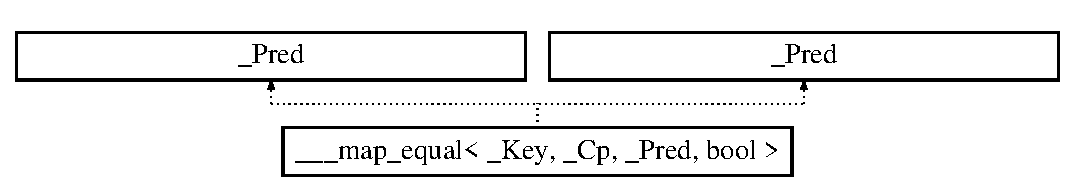
\includegraphics[height=2.000000cm]{class______map__equal}
\end{center}
\end{figure}
\subsection*{Public Member Functions}
\begin{DoxyCompactItemize}
\item 
\+\_\+\+L\+I\+B\+C\+P\+P\+\_\+\+I\+N\+L\+I\+N\+E\+\_\+\+V\+I\+S\+I\+B\+I\+L\+I\+T\+Y \hyperlink{class______map__equal_a95533cc0358047580fa982c3b2713bcc}{\+\_\+\+\_\+\+\_\+map\+\_\+equal} () \+\_\+\+N\+O\+E\+X\+C\+E\+P\+T\+\_\+(is\+\_\+nothrow\+\_\+default\+\_\+constructible$<$ \+\_\+\+Pred $>$
\item 
\+\_\+\+L\+I\+B\+C\+P\+P\+\_\+\+I\+N\+L\+I\+N\+E\+\_\+\+V\+I\+S\+I\+B\+I\+L\+I\+T\+Y \hyperlink{class______map__equal_ae2e9e62e4beb119f42aa20e2d2dc0f04}{\+\_\+\+\_\+\+\_\+map\+\_\+equal} (const \+\_\+\+Pred \&\+\_\+\+\_\+p) \+\_\+\+N\+O\+E\+X\+C\+E\+P\+T\+\_\+(is\+\_\+nothrow\+\_\+copy\+\_\+constructible$<$ \+\_\+\+Pred $>$
\item 
\+\_\+\+L\+I\+B\+C\+P\+P\+\_\+\+I\+N\+L\+I\+N\+E\+\_\+\+V\+I\+S\+I\+B\+I\+L\+I\+T\+Y const \+\_\+\+Pred \& \hyperlink{class______map__equal_add4420efffdc70c6b42be2aaaacbae2a}{key\+\_\+eq} () const \+\_\+\+N\+O\+E\+X\+C\+E\+P\+T
\item 
\+\_\+\+L\+I\+B\+C\+P\+P\+\_\+\+I\+N\+L\+I\+N\+E\+\_\+\+V\+I\+S\+I\+B\+I\+L\+I\+T\+Y bool \hyperlink{class______map__equal_a085532e0ec93fb5727e13db7881b1afd}{operator()} (const \+\_\+\+Cp \&\+\_\+\+\_\+x, const \+\_\+\+Cp \&\+\_\+\+\_\+y) const 
\item 
\+\_\+\+L\+I\+B\+C\+P\+P\+\_\+\+I\+N\+L\+I\+N\+E\+\_\+\+V\+I\+S\+I\+B\+I\+L\+I\+T\+Y bool \hyperlink{class______map__equal_a1bd9111ef0e0c36338fad7e015a635bb}{operator()} (const \+\_\+\+Cp \&\+\_\+\+\_\+x, const \+\_\+\+Key \&\+\_\+\+\_\+y) const 
\item 
\+\_\+\+L\+I\+B\+C\+P\+P\+\_\+\+I\+N\+L\+I\+N\+E\+\_\+\+V\+I\+S\+I\+B\+I\+L\+I\+T\+Y bool \hyperlink{class______map__equal_a8292b0d2bbe834c1f7de58b4e146f126}{operator()} (const \+\_\+\+Key \&\+\_\+\+\_\+x, const \+\_\+\+Cp \&\+\_\+\+\_\+y) const 
\item 
\+\_\+\+L\+I\+B\+C\+P\+P\+\_\+\+I\+N\+L\+I\+N\+E\+\_\+\+V\+I\+S\+I\+B\+I\+L\+I\+T\+Y \hyperlink{class______map__equal_a95533cc0358047580fa982c3b2713bcc}{\+\_\+\+\_\+\+\_\+map\+\_\+equal} () \+\_\+\+N\+O\+E\+X\+C\+E\+P\+T\+\_\+(is\+\_\+nothrow\+\_\+default\+\_\+constructible$<$ \+\_\+\+Pred $>$
\item 
\+\_\+\+L\+I\+B\+C\+P\+P\+\_\+\+I\+N\+L\+I\+N\+E\+\_\+\+V\+I\+S\+I\+B\+I\+L\+I\+T\+Y \hyperlink{class______map__equal_ae2e9e62e4beb119f42aa20e2d2dc0f04}{\+\_\+\+\_\+\+\_\+map\+\_\+equal} (const \+\_\+\+Pred \&\+\_\+\+\_\+p) \+\_\+\+N\+O\+E\+X\+C\+E\+P\+T\+\_\+(is\+\_\+nothrow\+\_\+copy\+\_\+constructible$<$ \+\_\+\+Pred $>$
\item 
\+\_\+\+L\+I\+B\+C\+P\+P\+\_\+\+I\+N\+L\+I\+N\+E\+\_\+\+V\+I\+S\+I\+B\+I\+L\+I\+T\+Y const \+\_\+\+Pred \& \hyperlink{class______map__equal_add4420efffdc70c6b42be2aaaacbae2a}{key\+\_\+eq} () const \+\_\+\+N\+O\+E\+X\+C\+E\+P\+T
\item 
\+\_\+\+L\+I\+B\+C\+P\+P\+\_\+\+I\+N\+L\+I\+N\+E\+\_\+\+V\+I\+S\+I\+B\+I\+L\+I\+T\+Y bool \hyperlink{class______map__equal_a085532e0ec93fb5727e13db7881b1afd}{operator()} (const \+\_\+\+Cp \&\+\_\+\+\_\+x, const \+\_\+\+Cp \&\+\_\+\+\_\+y) const 
\item 
\+\_\+\+L\+I\+B\+C\+P\+P\+\_\+\+I\+N\+L\+I\+N\+E\+\_\+\+V\+I\+S\+I\+B\+I\+L\+I\+T\+Y bool \hyperlink{class______map__equal_a1bd9111ef0e0c36338fad7e015a635bb}{operator()} (const \+\_\+\+Cp \&\+\_\+\+\_\+x, const \+\_\+\+Key \&\+\_\+\+\_\+y) const 
\item 
\+\_\+\+L\+I\+B\+C\+P\+P\+\_\+\+I\+N\+L\+I\+N\+E\+\_\+\+V\+I\+S\+I\+B\+I\+L\+I\+T\+Y bool \hyperlink{class______map__equal_a8292b0d2bbe834c1f7de58b4e146f126}{operator()} (const \+\_\+\+Key \&\+\_\+\+\_\+x, const \+\_\+\+Cp \&\+\_\+\+\_\+y) const 
\end{DoxyCompactItemize}


\subsection{Constructor \& Destructor Documentation}
\hypertarget{class______map__equal_a95533cc0358047580fa982c3b2713bcc}{}\index{\+\_\+\+\_\+\+\_\+map\+\_\+equal@{\+\_\+\+\_\+\+\_\+map\+\_\+equal}!\+\_\+\+\_\+\+\_\+map\+\_\+equal@{\+\_\+\+\_\+\+\_\+map\+\_\+equal}}
\index{\+\_\+\+\_\+\+\_\+map\+\_\+equal@{\+\_\+\+\_\+\+\_\+map\+\_\+equal}!\+\_\+\+\_\+\+\_\+map\+\_\+equal@{\+\_\+\+\_\+\+\_\+map\+\_\+equal}}
\subsubsection[{\+\_\+\+\_\+\+\_\+map\+\_\+equal() \+\_\+\+N\+O\+E\+X\+C\+E\+P\+T\+\_\+(is\+\_\+nothrow\+\_\+default\+\_\+constructible$<$ \+\_\+\+Pred $>$}]{\setlength{\rightskip}{0pt plus 5cm}template$<$class \+\_\+\+Key , class \+\_\+\+Cp , class \+\_\+\+Pred , bool  = is\+\_\+empty$<$\+\_\+\+Pred$>$\+::value$>$ \+\_\+\+L\+I\+B\+C\+P\+P\+\_\+\+I\+N\+L\+I\+N\+E\+\_\+\+V\+I\+S\+I\+B\+I\+L\+I\+T\+Y {\bf \+\_\+\+\_\+\+\_\+map\+\_\+equal}$<$ \+\_\+\+Key, \+\_\+\+Cp, \+\_\+\+Pred, bool $>$\+::{\bf \+\_\+\+\_\+\+\_\+map\+\_\+equal} (
\begin{DoxyParamCaption}
{}
\end{DoxyParamCaption}
)\hspace{0.3cm}{\ttfamily [inline]}}\label{class______map__equal_a95533cc0358047580fa982c3b2713bcc}
\hypertarget{class______map__equal_ae2e9e62e4beb119f42aa20e2d2dc0f04}{}\index{\+\_\+\+\_\+\+\_\+map\+\_\+equal@{\+\_\+\+\_\+\+\_\+map\+\_\+equal}!\+\_\+\+\_\+\+\_\+map\+\_\+equal@{\+\_\+\+\_\+\+\_\+map\+\_\+equal}}
\index{\+\_\+\+\_\+\+\_\+map\+\_\+equal@{\+\_\+\+\_\+\+\_\+map\+\_\+equal}!\+\_\+\+\_\+\+\_\+map\+\_\+equal@{\+\_\+\+\_\+\+\_\+map\+\_\+equal}}
\subsubsection[{\+\_\+\+\_\+\+\_\+map\+\_\+equal(const \+\_\+\+Pred \&\+\_\+\+\_\+p) \+\_\+\+N\+O\+E\+X\+C\+E\+P\+T\+\_\+(is\+\_\+nothrow\+\_\+copy\+\_\+constructible$<$ \+\_\+\+Pred $>$}]{\setlength{\rightskip}{0pt plus 5cm}template$<$class \+\_\+\+Key , class \+\_\+\+Cp , class \+\_\+\+Pred , bool  = is\+\_\+empty$<$\+\_\+\+Pred$>$\+::value$>$ \+\_\+\+L\+I\+B\+C\+P\+P\+\_\+\+I\+N\+L\+I\+N\+E\+\_\+\+V\+I\+S\+I\+B\+I\+L\+I\+T\+Y {\bf \+\_\+\+\_\+\+\_\+map\+\_\+equal}$<$ \+\_\+\+Key, \+\_\+\+Cp, \+\_\+\+Pred, bool $>$\+::{\bf \+\_\+\+\_\+\+\_\+map\+\_\+equal} (
\begin{DoxyParamCaption}
\item[{const \+\_\+\+Pred \&}]{\+\_\+\+\_\+p}
\end{DoxyParamCaption}
)\hspace{0.3cm}{\ttfamily [inline]}}\label{class______map__equal_ae2e9e62e4beb119f42aa20e2d2dc0f04}
\hypertarget{class______map__equal_a95533cc0358047580fa982c3b2713bcc}{}\index{\+\_\+\+\_\+\+\_\+map\+\_\+equal@{\+\_\+\+\_\+\+\_\+map\+\_\+equal}!\+\_\+\+\_\+\+\_\+map\+\_\+equal@{\+\_\+\+\_\+\+\_\+map\+\_\+equal}}
\index{\+\_\+\+\_\+\+\_\+map\+\_\+equal@{\+\_\+\+\_\+\+\_\+map\+\_\+equal}!\+\_\+\+\_\+\+\_\+map\+\_\+equal@{\+\_\+\+\_\+\+\_\+map\+\_\+equal}}
\subsubsection[{\+\_\+\+\_\+\+\_\+map\+\_\+equal() \+\_\+\+N\+O\+E\+X\+C\+E\+P\+T\+\_\+(is\+\_\+nothrow\+\_\+default\+\_\+constructible$<$ \+\_\+\+Pred $>$}]{\setlength{\rightskip}{0pt plus 5cm}template$<$class \+\_\+\+Key , class \+\_\+\+Cp , class \+\_\+\+Pred , bool  = is\+\_\+empty$<$\+\_\+\+Pred$>$\+::value$>$ \+\_\+\+L\+I\+B\+C\+P\+P\+\_\+\+I\+N\+L\+I\+N\+E\+\_\+\+V\+I\+S\+I\+B\+I\+L\+I\+T\+Y {\bf \+\_\+\+\_\+\+\_\+map\+\_\+equal}$<$ \+\_\+\+Key, \+\_\+\+Cp, \+\_\+\+Pred, bool $>$\+::{\bf \+\_\+\+\_\+\+\_\+map\+\_\+equal} (
\begin{DoxyParamCaption}
{}
\end{DoxyParamCaption}
)\hspace{0.3cm}{\ttfamily [inline]}}\label{class______map__equal_a95533cc0358047580fa982c3b2713bcc}
\hypertarget{class______map__equal_ae2e9e62e4beb119f42aa20e2d2dc0f04}{}\index{\+\_\+\+\_\+\+\_\+map\+\_\+equal@{\+\_\+\+\_\+\+\_\+map\+\_\+equal}!\+\_\+\+\_\+\+\_\+map\+\_\+equal@{\+\_\+\+\_\+\+\_\+map\+\_\+equal}}
\index{\+\_\+\+\_\+\+\_\+map\+\_\+equal@{\+\_\+\+\_\+\+\_\+map\+\_\+equal}!\+\_\+\+\_\+\+\_\+map\+\_\+equal@{\+\_\+\+\_\+\+\_\+map\+\_\+equal}}
\subsubsection[{\+\_\+\+\_\+\+\_\+map\+\_\+equal(const \+\_\+\+Pred \&\+\_\+\+\_\+p) \+\_\+\+N\+O\+E\+X\+C\+E\+P\+T\+\_\+(is\+\_\+nothrow\+\_\+copy\+\_\+constructible$<$ \+\_\+\+Pred $>$}]{\setlength{\rightskip}{0pt plus 5cm}template$<$class \+\_\+\+Key , class \+\_\+\+Cp , class \+\_\+\+Pred , bool  = is\+\_\+empty$<$\+\_\+\+Pred$>$\+::value$>$ \+\_\+\+L\+I\+B\+C\+P\+P\+\_\+\+I\+N\+L\+I\+N\+E\+\_\+\+V\+I\+S\+I\+B\+I\+L\+I\+T\+Y {\bf \+\_\+\+\_\+\+\_\+map\+\_\+equal}$<$ \+\_\+\+Key, \+\_\+\+Cp, \+\_\+\+Pred, bool $>$\+::{\bf \+\_\+\+\_\+\+\_\+map\+\_\+equal} (
\begin{DoxyParamCaption}
\item[{const \+\_\+\+Pred \&}]{\+\_\+\+\_\+p}
\end{DoxyParamCaption}
)\hspace{0.3cm}{\ttfamily [inline]}}\label{class______map__equal_ae2e9e62e4beb119f42aa20e2d2dc0f04}


\subsection{Member Function Documentation}
\hypertarget{class______map__equal_add4420efffdc70c6b42be2aaaacbae2a}{}\index{\+\_\+\+\_\+\+\_\+map\+\_\+equal@{\+\_\+\+\_\+\+\_\+map\+\_\+equal}!key\+\_\+eq@{key\+\_\+eq}}
\index{key\+\_\+eq@{key\+\_\+eq}!\+\_\+\+\_\+\+\_\+map\+\_\+equal@{\+\_\+\+\_\+\+\_\+map\+\_\+equal}}
\subsubsection[{key\+\_\+eq() const \+\_\+\+N\+O\+E\+X\+C\+E\+P\+T}]{\setlength{\rightskip}{0pt plus 5cm}template$<$class \+\_\+\+Key , class \+\_\+\+Cp , class \+\_\+\+Pred , bool  = is\+\_\+empty$<$\+\_\+\+Pred$>$\+::value$>$ \+\_\+\+L\+I\+B\+C\+P\+P\+\_\+\+I\+N\+L\+I\+N\+E\+\_\+\+V\+I\+S\+I\+B\+I\+L\+I\+T\+Y const \+\_\+\+Pred\& {\bf \+\_\+\+\_\+\+\_\+map\+\_\+equal}$<$ \+\_\+\+Key, \+\_\+\+Cp, \+\_\+\+Pred, bool $>$\+::key\+\_\+eq (
\begin{DoxyParamCaption}
{}
\end{DoxyParamCaption}
) const\hspace{0.3cm}{\ttfamily [inline]}}\label{class______map__equal_add4420efffdc70c6b42be2aaaacbae2a}
\hypertarget{class______map__equal_add4420efffdc70c6b42be2aaaacbae2a}{}\index{\+\_\+\+\_\+\+\_\+map\+\_\+equal@{\+\_\+\+\_\+\+\_\+map\+\_\+equal}!key\+\_\+eq@{key\+\_\+eq}}
\index{key\+\_\+eq@{key\+\_\+eq}!\+\_\+\+\_\+\+\_\+map\+\_\+equal@{\+\_\+\+\_\+\+\_\+map\+\_\+equal}}
\subsubsection[{key\+\_\+eq() const \+\_\+\+N\+O\+E\+X\+C\+E\+P\+T}]{\setlength{\rightskip}{0pt plus 5cm}template$<$class \+\_\+\+Key , class \+\_\+\+Cp , class \+\_\+\+Pred , bool  = is\+\_\+empty$<$\+\_\+\+Pred$>$\+::value$>$ \+\_\+\+L\+I\+B\+C\+P\+P\+\_\+\+I\+N\+L\+I\+N\+E\+\_\+\+V\+I\+S\+I\+B\+I\+L\+I\+T\+Y const \+\_\+\+Pred\& {\bf \+\_\+\+\_\+\+\_\+map\+\_\+equal}$<$ \+\_\+\+Key, \+\_\+\+Cp, \+\_\+\+Pred, bool $>$\+::key\+\_\+eq (
\begin{DoxyParamCaption}
{}
\end{DoxyParamCaption}
) const\hspace{0.3cm}{\ttfamily [inline]}}\label{class______map__equal_add4420efffdc70c6b42be2aaaacbae2a}
\hypertarget{class______map__equal_a085532e0ec93fb5727e13db7881b1afd}{}\index{\+\_\+\+\_\+\+\_\+map\+\_\+equal@{\+\_\+\+\_\+\+\_\+map\+\_\+equal}!operator()@{operator()}}
\index{operator()@{operator()}!\+\_\+\+\_\+\+\_\+map\+\_\+equal@{\+\_\+\+\_\+\+\_\+map\+\_\+equal}}
\subsubsection[{operator()(const \+\_\+\+Cp \&\+\_\+\+\_\+x, const \+\_\+\+Cp \&\+\_\+\+\_\+y) const }]{\setlength{\rightskip}{0pt plus 5cm}template$<$class \+\_\+\+Key , class \+\_\+\+Cp , class \+\_\+\+Pred , bool  = is\+\_\+empty$<$\+\_\+\+Pred$>$\+::value$>$ \+\_\+\+L\+I\+B\+C\+P\+P\+\_\+\+I\+N\+L\+I\+N\+E\+\_\+\+V\+I\+S\+I\+B\+I\+L\+I\+T\+Y bool {\bf \+\_\+\+\_\+\+\_\+map\+\_\+equal}$<$ \+\_\+\+Key, \+\_\+\+Cp, \+\_\+\+Pred, bool $>$\+::operator() (
\begin{DoxyParamCaption}
\item[{const \+\_\+\+Cp \&}]{\+\_\+\+\_\+x, }
\item[{const \+\_\+\+Cp \&}]{\+\_\+\+\_\+y}
\end{DoxyParamCaption}
) const\hspace{0.3cm}{\ttfamily [inline]}}\label{class______map__equal_a085532e0ec93fb5727e13db7881b1afd}
\hypertarget{class______map__equal_a085532e0ec93fb5727e13db7881b1afd}{}\index{\+\_\+\+\_\+\+\_\+map\+\_\+equal@{\+\_\+\+\_\+\+\_\+map\+\_\+equal}!operator()@{operator()}}
\index{operator()@{operator()}!\+\_\+\+\_\+\+\_\+map\+\_\+equal@{\+\_\+\+\_\+\+\_\+map\+\_\+equal}}
\subsubsection[{operator()(const \+\_\+\+Cp \&\+\_\+\+\_\+x, const \+\_\+\+Cp \&\+\_\+\+\_\+y) const }]{\setlength{\rightskip}{0pt plus 5cm}template$<$class \+\_\+\+Key , class \+\_\+\+Cp , class \+\_\+\+Pred , bool  = is\+\_\+empty$<$\+\_\+\+Pred$>$\+::value$>$ \+\_\+\+L\+I\+B\+C\+P\+P\+\_\+\+I\+N\+L\+I\+N\+E\+\_\+\+V\+I\+S\+I\+B\+I\+L\+I\+T\+Y bool {\bf \+\_\+\+\_\+\+\_\+map\+\_\+equal}$<$ \+\_\+\+Key, \+\_\+\+Cp, \+\_\+\+Pred, bool $>$\+::operator() (
\begin{DoxyParamCaption}
\item[{const \+\_\+\+Cp \&}]{\+\_\+\+\_\+x, }
\item[{const \+\_\+\+Cp \&}]{\+\_\+\+\_\+y}
\end{DoxyParamCaption}
) const\hspace{0.3cm}{\ttfamily [inline]}}\label{class______map__equal_a085532e0ec93fb5727e13db7881b1afd}
\hypertarget{class______map__equal_a1bd9111ef0e0c36338fad7e015a635bb}{}\index{\+\_\+\+\_\+\+\_\+map\+\_\+equal@{\+\_\+\+\_\+\+\_\+map\+\_\+equal}!operator()@{operator()}}
\index{operator()@{operator()}!\+\_\+\+\_\+\+\_\+map\+\_\+equal@{\+\_\+\+\_\+\+\_\+map\+\_\+equal}}
\subsubsection[{operator()(const \+\_\+\+Cp \&\+\_\+\+\_\+x, const \+\_\+\+Key \&\+\_\+\+\_\+y) const }]{\setlength{\rightskip}{0pt plus 5cm}template$<$class \+\_\+\+Key , class \+\_\+\+Cp , class \+\_\+\+Pred , bool  = is\+\_\+empty$<$\+\_\+\+Pred$>$\+::value$>$ \+\_\+\+L\+I\+B\+C\+P\+P\+\_\+\+I\+N\+L\+I\+N\+E\+\_\+\+V\+I\+S\+I\+B\+I\+L\+I\+T\+Y bool {\bf \+\_\+\+\_\+\+\_\+map\+\_\+equal}$<$ \+\_\+\+Key, \+\_\+\+Cp, \+\_\+\+Pred, bool $>$\+::operator() (
\begin{DoxyParamCaption}
\item[{const \+\_\+\+Cp \&}]{\+\_\+\+\_\+x, }
\item[{const \+\_\+\+Key \&}]{\+\_\+\+\_\+y}
\end{DoxyParamCaption}
) const\hspace{0.3cm}{\ttfamily [inline]}}\label{class______map__equal_a1bd9111ef0e0c36338fad7e015a635bb}
\hypertarget{class______map__equal_a8292b0d2bbe834c1f7de58b4e146f126}{}\index{\+\_\+\+\_\+\+\_\+map\+\_\+equal@{\+\_\+\+\_\+\+\_\+map\+\_\+equal}!operator()@{operator()}}
\index{operator()@{operator()}!\+\_\+\+\_\+\+\_\+map\+\_\+equal@{\+\_\+\+\_\+\+\_\+map\+\_\+equal}}
\subsubsection[{operator()(const \+\_\+\+Key \&\+\_\+\+\_\+x, const \+\_\+\+Cp \&\+\_\+\+\_\+y) const }]{\setlength{\rightskip}{0pt plus 5cm}template$<$class \+\_\+\+Key , class \+\_\+\+Cp , class \+\_\+\+Pred , bool  = is\+\_\+empty$<$\+\_\+\+Pred$>$\+::value$>$ \+\_\+\+L\+I\+B\+C\+P\+P\+\_\+\+I\+N\+L\+I\+N\+E\+\_\+\+V\+I\+S\+I\+B\+I\+L\+I\+T\+Y bool {\bf \+\_\+\+\_\+\+\_\+map\+\_\+equal}$<$ \+\_\+\+Key, \+\_\+\+Cp, \+\_\+\+Pred, bool $>$\+::operator() (
\begin{DoxyParamCaption}
\item[{const \+\_\+\+Key \&}]{\+\_\+\+\_\+x, }
\item[{const \+\_\+\+Cp \&}]{\+\_\+\+\_\+y}
\end{DoxyParamCaption}
) const\hspace{0.3cm}{\ttfamily [inline]}}\label{class______map__equal_a8292b0d2bbe834c1f7de58b4e146f126}
\hypertarget{class______map__equal_a1bd9111ef0e0c36338fad7e015a635bb}{}\index{\+\_\+\+\_\+\+\_\+map\+\_\+equal@{\+\_\+\+\_\+\+\_\+map\+\_\+equal}!operator()@{operator()}}
\index{operator()@{operator()}!\+\_\+\+\_\+\+\_\+map\+\_\+equal@{\+\_\+\+\_\+\+\_\+map\+\_\+equal}}
\subsubsection[{operator()(const \+\_\+\+Cp \&\+\_\+\+\_\+x, const \+\_\+\+Key \&\+\_\+\+\_\+y) const }]{\setlength{\rightskip}{0pt plus 5cm}template$<$class \+\_\+\+Key , class \+\_\+\+Cp , class \+\_\+\+Pred , bool  = is\+\_\+empty$<$\+\_\+\+Pred$>$\+::value$>$ \+\_\+\+L\+I\+B\+C\+P\+P\+\_\+\+I\+N\+L\+I\+N\+E\+\_\+\+V\+I\+S\+I\+B\+I\+L\+I\+T\+Y bool {\bf \+\_\+\+\_\+\+\_\+map\+\_\+equal}$<$ \+\_\+\+Key, \+\_\+\+Cp, \+\_\+\+Pred, bool $>$\+::operator() (
\begin{DoxyParamCaption}
\item[{const \+\_\+\+Cp \&}]{\+\_\+\+\_\+x, }
\item[{const \+\_\+\+Key \&}]{\+\_\+\+\_\+y}
\end{DoxyParamCaption}
) const\hspace{0.3cm}{\ttfamily [inline]}}\label{class______map__equal_a1bd9111ef0e0c36338fad7e015a635bb}
\hypertarget{class______map__equal_a8292b0d2bbe834c1f7de58b4e146f126}{}\index{\+\_\+\+\_\+\+\_\+map\+\_\+equal@{\+\_\+\+\_\+\+\_\+map\+\_\+equal}!operator()@{operator()}}
\index{operator()@{operator()}!\+\_\+\+\_\+\+\_\+map\+\_\+equal@{\+\_\+\+\_\+\+\_\+map\+\_\+equal}}
\subsubsection[{operator()(const \+\_\+\+Key \&\+\_\+\+\_\+x, const \+\_\+\+Cp \&\+\_\+\+\_\+y) const }]{\setlength{\rightskip}{0pt plus 5cm}template$<$class \+\_\+\+Key , class \+\_\+\+Cp , class \+\_\+\+Pred , bool  = is\+\_\+empty$<$\+\_\+\+Pred$>$\+::value$>$ \+\_\+\+L\+I\+B\+C\+P\+P\+\_\+\+I\+N\+L\+I\+N\+E\+\_\+\+V\+I\+S\+I\+B\+I\+L\+I\+T\+Y bool {\bf \+\_\+\+\_\+\+\_\+map\+\_\+equal}$<$ \+\_\+\+Key, \+\_\+\+Cp, \+\_\+\+Pred, bool $>$\+::operator() (
\begin{DoxyParamCaption}
\item[{const \+\_\+\+Key \&}]{\+\_\+\+\_\+x, }
\item[{const \+\_\+\+Cp \&}]{\+\_\+\+\_\+y}
\end{DoxyParamCaption}
) const\hspace{0.3cm}{\ttfamily [inline]}}\label{class______map__equal_a8292b0d2bbe834c1f7de58b4e146f126}


The documentation for this class was generated from the following files\+:\begin{DoxyCompactItemize}
\item 
/\+Users/brandonmcfarland/\+Desktop/searchdocs/\+Search\+Engine/\+Final\+Project/\hyperlink{mapping_8cpp}{mapping.\+cpp}\item 
/\+Users/brandonmcfarland/\+Desktop/searchdocs/\+Search\+Engine/\+Final\+Project/\hyperlink{mapping_8h}{mapping.\+h}\end{DoxyCompactItemize}

\hypertarget{class______map__equal_3_01___key_00_01___cp_00_01___pred_00_01false_01_4}{}\section{\+\_\+\+\_\+\+\_\+map\+\_\+equal$<$ \+\_\+\+Key, \+\_\+\+Cp, \+\_\+\+Pred, false $>$ Class Template Reference}
\label{class______map__equal_3_01___key_00_01___cp_00_01___pred_00_01false_01_4}\index{\+\_\+\+\_\+\+\_\+map\+\_\+equal$<$ \+\_\+\+Key, \+\_\+\+Cp, \+\_\+\+Pred, false $>$@{\+\_\+\+\_\+\+\_\+map\+\_\+equal$<$ \+\_\+\+Key, \+\_\+\+Cp, \+\_\+\+Pred, false $>$}}


{\ttfamily \#include $<$mapping.\+h$>$}

\subsection*{Public Member Functions}
\begin{DoxyCompactItemize}
\item 
\+\_\+\+L\+I\+B\+C\+P\+P\+\_\+\+I\+N\+L\+I\+N\+E\+\_\+\+V\+I\+S\+I\+B\+I\+L\+I\+T\+Y \hyperlink{class______map__equal_3_01___key_00_01___cp_00_01___pred_00_01false_01_4_a58d140185db242b2e905f1e094957896}{\+\_\+\+\_\+\+\_\+map\+\_\+equal} () \+\_\+\+N\+O\+E\+X\+C\+E\+P\+T\+\_\+(is\+\_\+nothrow\+\_\+default\+\_\+constructible$<$ \+\_\+\+Pred $>$
\item 
\+\_\+\+L\+I\+B\+C\+P\+P\+\_\+\+I\+N\+L\+I\+N\+E\+\_\+\+V\+I\+S\+I\+B\+I\+L\+I\+T\+Y \hyperlink{class______map__equal_3_01___key_00_01___cp_00_01___pred_00_01false_01_4_a20796310662e2eb592cacef4385b3223}{\+\_\+\+\_\+\+\_\+map\+\_\+equal} (const \+\_\+\+Pred \&\+\_\+\+\_\+p) \+\_\+\+N\+O\+E\+X\+C\+E\+P\+T\+\_\+(is\+\_\+nothrow\+\_\+copy\+\_\+constructible$<$ \+\_\+\+Pred $>$
\item 
\+\_\+\+L\+I\+B\+C\+P\+P\+\_\+\+I\+N\+L\+I\+N\+E\+\_\+\+V\+I\+S\+I\+B\+I\+L\+I\+T\+Y const \+\_\+\+Pred \& \hyperlink{class______map__equal_3_01___key_00_01___cp_00_01___pred_00_01false_01_4_a3bf1ce76006942fec62d148d68ac498b}{key\+\_\+eq} () const \+\_\+\+N\+O\+E\+X\+C\+E\+P\+T
\item 
\+\_\+\+L\+I\+B\+C\+P\+P\+\_\+\+I\+N\+L\+I\+N\+E\+\_\+\+V\+I\+S\+I\+B\+I\+L\+I\+T\+Y bool \hyperlink{class______map__equal_3_01___key_00_01___cp_00_01___pred_00_01false_01_4_a610f1a9c10d40791c098fe1af3beaf57}{operator()} (const \+\_\+\+Cp \&\+\_\+\+\_\+x, const \+\_\+\+Cp \&\+\_\+\+\_\+y) const 
\item 
\+\_\+\+L\+I\+B\+C\+P\+P\+\_\+\+I\+N\+L\+I\+N\+E\+\_\+\+V\+I\+S\+I\+B\+I\+L\+I\+T\+Y bool \hyperlink{class______map__equal_3_01___key_00_01___cp_00_01___pred_00_01false_01_4_af3ff9fb13ef0c4d455bdd274adf3b579}{operator()} (const \+\_\+\+Cp \&\+\_\+\+\_\+x, const \+\_\+\+Key \&\+\_\+\+\_\+y) const 
\item 
\+\_\+\+L\+I\+B\+C\+P\+P\+\_\+\+I\+N\+L\+I\+N\+E\+\_\+\+V\+I\+S\+I\+B\+I\+L\+I\+T\+Y bool \hyperlink{class______map__equal_3_01___key_00_01___cp_00_01___pred_00_01false_01_4_a2ae80d5d4f0899ce42eac8bba386eb9c}{operator()} (const \+\_\+\+Key \&\+\_\+\+\_\+x, const \+\_\+\+Cp \&\+\_\+\+\_\+y) const 
\item 
\+\_\+\+L\+I\+B\+C\+P\+P\+\_\+\+I\+N\+L\+I\+N\+E\+\_\+\+V\+I\+S\+I\+B\+I\+L\+I\+T\+Y \hyperlink{class______map__equal_3_01___key_00_01___cp_00_01___pred_00_01false_01_4_a58d140185db242b2e905f1e094957896}{\+\_\+\+\_\+\+\_\+map\+\_\+equal} () \+\_\+\+N\+O\+E\+X\+C\+E\+P\+T\+\_\+(is\+\_\+nothrow\+\_\+default\+\_\+constructible$<$ \+\_\+\+Pred $>$
\item 
\+\_\+\+L\+I\+B\+C\+P\+P\+\_\+\+I\+N\+L\+I\+N\+E\+\_\+\+V\+I\+S\+I\+B\+I\+L\+I\+T\+Y \hyperlink{class______map__equal_3_01___key_00_01___cp_00_01___pred_00_01false_01_4_a20796310662e2eb592cacef4385b3223}{\+\_\+\+\_\+\+\_\+map\+\_\+equal} (const \+\_\+\+Pred \&\+\_\+\+\_\+p) \+\_\+\+N\+O\+E\+X\+C\+E\+P\+T\+\_\+(is\+\_\+nothrow\+\_\+copy\+\_\+constructible$<$ \+\_\+\+Pred $>$
\item 
\+\_\+\+L\+I\+B\+C\+P\+P\+\_\+\+I\+N\+L\+I\+N\+E\+\_\+\+V\+I\+S\+I\+B\+I\+L\+I\+T\+Y const \+\_\+\+Pred \& \hyperlink{class______map__equal_3_01___key_00_01___cp_00_01___pred_00_01false_01_4_a3bf1ce76006942fec62d148d68ac498b}{key\+\_\+eq} () const \+\_\+\+N\+O\+E\+X\+C\+E\+P\+T
\item 
\+\_\+\+L\+I\+B\+C\+P\+P\+\_\+\+I\+N\+L\+I\+N\+E\+\_\+\+V\+I\+S\+I\+B\+I\+L\+I\+T\+Y bool \hyperlink{class______map__equal_3_01___key_00_01___cp_00_01___pred_00_01false_01_4_a610f1a9c10d40791c098fe1af3beaf57}{operator()} (const \+\_\+\+Cp \&\+\_\+\+\_\+x, const \+\_\+\+Cp \&\+\_\+\+\_\+y) const 
\item 
\+\_\+\+L\+I\+B\+C\+P\+P\+\_\+\+I\+N\+L\+I\+N\+E\+\_\+\+V\+I\+S\+I\+B\+I\+L\+I\+T\+Y bool \hyperlink{class______map__equal_3_01___key_00_01___cp_00_01___pred_00_01false_01_4_af3ff9fb13ef0c4d455bdd274adf3b579}{operator()} (const \+\_\+\+Cp \&\+\_\+\+\_\+x, const \+\_\+\+Key \&\+\_\+\+\_\+y) const 
\item 
\+\_\+\+L\+I\+B\+C\+P\+P\+\_\+\+I\+N\+L\+I\+N\+E\+\_\+\+V\+I\+S\+I\+B\+I\+L\+I\+T\+Y bool \hyperlink{class______map__equal_3_01___key_00_01___cp_00_01___pred_00_01false_01_4_a2ae80d5d4f0899ce42eac8bba386eb9c}{operator()} (const \+\_\+\+Key \&\+\_\+\+\_\+x, const \+\_\+\+Cp \&\+\_\+\+\_\+y) const 
\end{DoxyCompactItemize}


\subsection{Constructor \& Destructor Documentation}
\hypertarget{class______map__equal_3_01___key_00_01___cp_00_01___pred_00_01false_01_4_a58d140185db242b2e905f1e094957896}{}\index{\+\_\+\+\_\+\+\_\+map\+\_\+equal$<$ \+\_\+\+Key, \+\_\+\+Cp, \+\_\+\+Pred, false $>$@{\+\_\+\+\_\+\+\_\+map\+\_\+equal$<$ \+\_\+\+Key, \+\_\+\+Cp, \+\_\+\+Pred, false $>$}!\+\_\+\+\_\+\+\_\+map\+\_\+equal@{\+\_\+\+\_\+\+\_\+map\+\_\+equal}}
\index{\+\_\+\+\_\+\+\_\+map\+\_\+equal@{\+\_\+\+\_\+\+\_\+map\+\_\+equal}!\+\_\+\+\_\+\+\_\+map\+\_\+equal$<$ \+\_\+\+Key, \+\_\+\+Cp, \+\_\+\+Pred, false $>$@{\+\_\+\+\_\+\+\_\+map\+\_\+equal$<$ \+\_\+\+Key, \+\_\+\+Cp, \+\_\+\+Pred, false $>$}}
\subsubsection[{\+\_\+\+\_\+\+\_\+map\+\_\+equal() \+\_\+\+N\+O\+E\+X\+C\+E\+P\+T\+\_\+(is\+\_\+nothrow\+\_\+default\+\_\+constructible$<$ \+\_\+\+Pred $>$}]{\setlength{\rightskip}{0pt plus 5cm}template$<$class \+\_\+\+Key , class \+\_\+\+Cp , class \+\_\+\+Pred $>$ \+\_\+\+L\+I\+B\+C\+P\+P\+\_\+\+I\+N\+L\+I\+N\+E\+\_\+\+V\+I\+S\+I\+B\+I\+L\+I\+T\+Y {\bf \+\_\+\+\_\+\+\_\+map\+\_\+equal}$<$ \+\_\+\+Key, \+\_\+\+Cp, \+\_\+\+Pred, false $>$\+::{\bf \+\_\+\+\_\+\+\_\+map\+\_\+equal} (
\begin{DoxyParamCaption}
{}
\end{DoxyParamCaption}
)\hspace{0.3cm}{\ttfamily [inline]}}\label{class______map__equal_3_01___key_00_01___cp_00_01___pred_00_01false_01_4_a58d140185db242b2e905f1e094957896}
\hypertarget{class______map__equal_3_01___key_00_01___cp_00_01___pred_00_01false_01_4_a20796310662e2eb592cacef4385b3223}{}\index{\+\_\+\+\_\+\+\_\+map\+\_\+equal$<$ \+\_\+\+Key, \+\_\+\+Cp, \+\_\+\+Pred, false $>$@{\+\_\+\+\_\+\+\_\+map\+\_\+equal$<$ \+\_\+\+Key, \+\_\+\+Cp, \+\_\+\+Pred, false $>$}!\+\_\+\+\_\+\+\_\+map\+\_\+equal@{\+\_\+\+\_\+\+\_\+map\+\_\+equal}}
\index{\+\_\+\+\_\+\+\_\+map\+\_\+equal@{\+\_\+\+\_\+\+\_\+map\+\_\+equal}!\+\_\+\+\_\+\+\_\+map\+\_\+equal$<$ \+\_\+\+Key, \+\_\+\+Cp, \+\_\+\+Pred, false $>$@{\+\_\+\+\_\+\+\_\+map\+\_\+equal$<$ \+\_\+\+Key, \+\_\+\+Cp, \+\_\+\+Pred, false $>$}}
\subsubsection[{\+\_\+\+\_\+\+\_\+map\+\_\+equal(const \+\_\+\+Pred \&\+\_\+\+\_\+p) \+\_\+\+N\+O\+E\+X\+C\+E\+P\+T\+\_\+(is\+\_\+nothrow\+\_\+copy\+\_\+constructible$<$ \+\_\+\+Pred $>$}]{\setlength{\rightskip}{0pt plus 5cm}template$<$class \+\_\+\+Key , class \+\_\+\+Cp , class \+\_\+\+Pred $>$ \+\_\+\+L\+I\+B\+C\+P\+P\+\_\+\+I\+N\+L\+I\+N\+E\+\_\+\+V\+I\+S\+I\+B\+I\+L\+I\+T\+Y {\bf \+\_\+\+\_\+\+\_\+map\+\_\+equal}$<$ \+\_\+\+Key, \+\_\+\+Cp, \+\_\+\+Pred, false $>$\+::{\bf \+\_\+\+\_\+\+\_\+map\+\_\+equal} (
\begin{DoxyParamCaption}
\item[{const \+\_\+\+Pred \&}]{\+\_\+\+\_\+p}
\end{DoxyParamCaption}
)\hspace{0.3cm}{\ttfamily [inline]}}\label{class______map__equal_3_01___key_00_01___cp_00_01___pred_00_01false_01_4_a20796310662e2eb592cacef4385b3223}
\hypertarget{class______map__equal_3_01___key_00_01___cp_00_01___pred_00_01false_01_4_a58d140185db242b2e905f1e094957896}{}\index{\+\_\+\+\_\+\+\_\+map\+\_\+equal$<$ \+\_\+\+Key, \+\_\+\+Cp, \+\_\+\+Pred, false $>$@{\+\_\+\+\_\+\+\_\+map\+\_\+equal$<$ \+\_\+\+Key, \+\_\+\+Cp, \+\_\+\+Pred, false $>$}!\+\_\+\+\_\+\+\_\+map\+\_\+equal@{\+\_\+\+\_\+\+\_\+map\+\_\+equal}}
\index{\+\_\+\+\_\+\+\_\+map\+\_\+equal@{\+\_\+\+\_\+\+\_\+map\+\_\+equal}!\+\_\+\+\_\+\+\_\+map\+\_\+equal$<$ \+\_\+\+Key, \+\_\+\+Cp, \+\_\+\+Pred, false $>$@{\+\_\+\+\_\+\+\_\+map\+\_\+equal$<$ \+\_\+\+Key, \+\_\+\+Cp, \+\_\+\+Pred, false $>$}}
\subsubsection[{\+\_\+\+\_\+\+\_\+map\+\_\+equal() \+\_\+\+N\+O\+E\+X\+C\+E\+P\+T\+\_\+(is\+\_\+nothrow\+\_\+default\+\_\+constructible$<$ \+\_\+\+Pred $>$}]{\setlength{\rightskip}{0pt plus 5cm}template$<$class \+\_\+\+Key , class \+\_\+\+Cp , class \+\_\+\+Pred $>$ \+\_\+\+L\+I\+B\+C\+P\+P\+\_\+\+I\+N\+L\+I\+N\+E\+\_\+\+V\+I\+S\+I\+B\+I\+L\+I\+T\+Y {\bf \+\_\+\+\_\+\+\_\+map\+\_\+equal}$<$ \+\_\+\+Key, \+\_\+\+Cp, \+\_\+\+Pred, false $>$\+::{\bf \+\_\+\+\_\+\+\_\+map\+\_\+equal} (
\begin{DoxyParamCaption}
{}
\end{DoxyParamCaption}
)\hspace{0.3cm}{\ttfamily [inline]}}\label{class______map__equal_3_01___key_00_01___cp_00_01___pred_00_01false_01_4_a58d140185db242b2e905f1e094957896}
\hypertarget{class______map__equal_3_01___key_00_01___cp_00_01___pred_00_01false_01_4_a20796310662e2eb592cacef4385b3223}{}\index{\+\_\+\+\_\+\+\_\+map\+\_\+equal$<$ \+\_\+\+Key, \+\_\+\+Cp, \+\_\+\+Pred, false $>$@{\+\_\+\+\_\+\+\_\+map\+\_\+equal$<$ \+\_\+\+Key, \+\_\+\+Cp, \+\_\+\+Pred, false $>$}!\+\_\+\+\_\+\+\_\+map\+\_\+equal@{\+\_\+\+\_\+\+\_\+map\+\_\+equal}}
\index{\+\_\+\+\_\+\+\_\+map\+\_\+equal@{\+\_\+\+\_\+\+\_\+map\+\_\+equal}!\+\_\+\+\_\+\+\_\+map\+\_\+equal$<$ \+\_\+\+Key, \+\_\+\+Cp, \+\_\+\+Pred, false $>$@{\+\_\+\+\_\+\+\_\+map\+\_\+equal$<$ \+\_\+\+Key, \+\_\+\+Cp, \+\_\+\+Pred, false $>$}}
\subsubsection[{\+\_\+\+\_\+\+\_\+map\+\_\+equal(const \+\_\+\+Pred \&\+\_\+\+\_\+p) \+\_\+\+N\+O\+E\+X\+C\+E\+P\+T\+\_\+(is\+\_\+nothrow\+\_\+copy\+\_\+constructible$<$ \+\_\+\+Pred $>$}]{\setlength{\rightskip}{0pt plus 5cm}template$<$class \+\_\+\+Key , class \+\_\+\+Cp , class \+\_\+\+Pred $>$ \+\_\+\+L\+I\+B\+C\+P\+P\+\_\+\+I\+N\+L\+I\+N\+E\+\_\+\+V\+I\+S\+I\+B\+I\+L\+I\+T\+Y {\bf \+\_\+\+\_\+\+\_\+map\+\_\+equal}$<$ \+\_\+\+Key, \+\_\+\+Cp, \+\_\+\+Pred, false $>$\+::{\bf \+\_\+\+\_\+\+\_\+map\+\_\+equal} (
\begin{DoxyParamCaption}
\item[{const \+\_\+\+Pred \&}]{\+\_\+\+\_\+p}
\end{DoxyParamCaption}
)\hspace{0.3cm}{\ttfamily [inline]}}\label{class______map__equal_3_01___key_00_01___cp_00_01___pred_00_01false_01_4_a20796310662e2eb592cacef4385b3223}


\subsection{Member Function Documentation}
\hypertarget{class______map__equal_3_01___key_00_01___cp_00_01___pred_00_01false_01_4_a3bf1ce76006942fec62d148d68ac498b}{}\index{\+\_\+\+\_\+\+\_\+map\+\_\+equal$<$ \+\_\+\+Key, \+\_\+\+Cp, \+\_\+\+Pred, false $>$@{\+\_\+\+\_\+\+\_\+map\+\_\+equal$<$ \+\_\+\+Key, \+\_\+\+Cp, \+\_\+\+Pred, false $>$}!key\+\_\+eq@{key\+\_\+eq}}
\index{key\+\_\+eq@{key\+\_\+eq}!\+\_\+\+\_\+\+\_\+map\+\_\+equal$<$ \+\_\+\+Key, \+\_\+\+Cp, \+\_\+\+Pred, false $>$@{\+\_\+\+\_\+\+\_\+map\+\_\+equal$<$ \+\_\+\+Key, \+\_\+\+Cp, \+\_\+\+Pred, false $>$}}
\subsubsection[{key\+\_\+eq() const \+\_\+\+N\+O\+E\+X\+C\+E\+P\+T}]{\setlength{\rightskip}{0pt plus 5cm}template$<$class \+\_\+\+Key , class \+\_\+\+Cp , class \+\_\+\+Pred $>$ \+\_\+\+L\+I\+B\+C\+P\+P\+\_\+\+I\+N\+L\+I\+N\+E\+\_\+\+V\+I\+S\+I\+B\+I\+L\+I\+T\+Y const \+\_\+\+Pred\& {\bf \+\_\+\+\_\+\+\_\+map\+\_\+equal}$<$ \+\_\+\+Key, \+\_\+\+Cp, \+\_\+\+Pred, false $>$\+::key\+\_\+eq (
\begin{DoxyParamCaption}
{}
\end{DoxyParamCaption}
) const\hspace{0.3cm}{\ttfamily [inline]}}\label{class______map__equal_3_01___key_00_01___cp_00_01___pred_00_01false_01_4_a3bf1ce76006942fec62d148d68ac498b}
\hypertarget{class______map__equal_3_01___key_00_01___cp_00_01___pred_00_01false_01_4_a3bf1ce76006942fec62d148d68ac498b}{}\index{\+\_\+\+\_\+\+\_\+map\+\_\+equal$<$ \+\_\+\+Key, \+\_\+\+Cp, \+\_\+\+Pred, false $>$@{\+\_\+\+\_\+\+\_\+map\+\_\+equal$<$ \+\_\+\+Key, \+\_\+\+Cp, \+\_\+\+Pred, false $>$}!key\+\_\+eq@{key\+\_\+eq}}
\index{key\+\_\+eq@{key\+\_\+eq}!\+\_\+\+\_\+\+\_\+map\+\_\+equal$<$ \+\_\+\+Key, \+\_\+\+Cp, \+\_\+\+Pred, false $>$@{\+\_\+\+\_\+\+\_\+map\+\_\+equal$<$ \+\_\+\+Key, \+\_\+\+Cp, \+\_\+\+Pred, false $>$}}
\subsubsection[{key\+\_\+eq() const \+\_\+\+N\+O\+E\+X\+C\+E\+P\+T}]{\setlength{\rightskip}{0pt plus 5cm}template$<$class \+\_\+\+Key , class \+\_\+\+Cp , class \+\_\+\+Pred $>$ \+\_\+\+L\+I\+B\+C\+P\+P\+\_\+\+I\+N\+L\+I\+N\+E\+\_\+\+V\+I\+S\+I\+B\+I\+L\+I\+T\+Y const \+\_\+\+Pred\& {\bf \+\_\+\+\_\+\+\_\+map\+\_\+equal}$<$ \+\_\+\+Key, \+\_\+\+Cp, \+\_\+\+Pred, false $>$\+::key\+\_\+eq (
\begin{DoxyParamCaption}
{}
\end{DoxyParamCaption}
) const\hspace{0.3cm}{\ttfamily [inline]}}\label{class______map__equal_3_01___key_00_01___cp_00_01___pred_00_01false_01_4_a3bf1ce76006942fec62d148d68ac498b}
\hypertarget{class______map__equal_3_01___key_00_01___cp_00_01___pred_00_01false_01_4_a610f1a9c10d40791c098fe1af3beaf57}{}\index{\+\_\+\+\_\+\+\_\+map\+\_\+equal$<$ \+\_\+\+Key, \+\_\+\+Cp, \+\_\+\+Pred, false $>$@{\+\_\+\+\_\+\+\_\+map\+\_\+equal$<$ \+\_\+\+Key, \+\_\+\+Cp, \+\_\+\+Pred, false $>$}!operator()@{operator()}}
\index{operator()@{operator()}!\+\_\+\+\_\+\+\_\+map\+\_\+equal$<$ \+\_\+\+Key, \+\_\+\+Cp, \+\_\+\+Pred, false $>$@{\+\_\+\+\_\+\+\_\+map\+\_\+equal$<$ \+\_\+\+Key, \+\_\+\+Cp, \+\_\+\+Pred, false $>$}}
\subsubsection[{operator()(const \+\_\+\+Cp \&\+\_\+\+\_\+x, const \+\_\+\+Cp \&\+\_\+\+\_\+y) const }]{\setlength{\rightskip}{0pt plus 5cm}template$<$class \+\_\+\+Key , class \+\_\+\+Cp , class \+\_\+\+Pred $>$ \+\_\+\+L\+I\+B\+C\+P\+P\+\_\+\+I\+N\+L\+I\+N\+E\+\_\+\+V\+I\+S\+I\+B\+I\+L\+I\+T\+Y bool {\bf \+\_\+\+\_\+\+\_\+map\+\_\+equal}$<$ \+\_\+\+Key, \+\_\+\+Cp, \+\_\+\+Pred, false $>$\+::operator() (
\begin{DoxyParamCaption}
\item[{const \+\_\+\+Cp \&}]{\+\_\+\+\_\+x, }
\item[{const \+\_\+\+Cp \&}]{\+\_\+\+\_\+y}
\end{DoxyParamCaption}
) const\hspace{0.3cm}{\ttfamily [inline]}}\label{class______map__equal_3_01___key_00_01___cp_00_01___pred_00_01false_01_4_a610f1a9c10d40791c098fe1af3beaf57}
\hypertarget{class______map__equal_3_01___key_00_01___cp_00_01___pred_00_01false_01_4_a610f1a9c10d40791c098fe1af3beaf57}{}\index{\+\_\+\+\_\+\+\_\+map\+\_\+equal$<$ \+\_\+\+Key, \+\_\+\+Cp, \+\_\+\+Pred, false $>$@{\+\_\+\+\_\+\+\_\+map\+\_\+equal$<$ \+\_\+\+Key, \+\_\+\+Cp, \+\_\+\+Pred, false $>$}!operator()@{operator()}}
\index{operator()@{operator()}!\+\_\+\+\_\+\+\_\+map\+\_\+equal$<$ \+\_\+\+Key, \+\_\+\+Cp, \+\_\+\+Pred, false $>$@{\+\_\+\+\_\+\+\_\+map\+\_\+equal$<$ \+\_\+\+Key, \+\_\+\+Cp, \+\_\+\+Pred, false $>$}}
\subsubsection[{operator()(const \+\_\+\+Cp \&\+\_\+\+\_\+x, const \+\_\+\+Cp \&\+\_\+\+\_\+y) const }]{\setlength{\rightskip}{0pt plus 5cm}template$<$class \+\_\+\+Key , class \+\_\+\+Cp , class \+\_\+\+Pred $>$ \+\_\+\+L\+I\+B\+C\+P\+P\+\_\+\+I\+N\+L\+I\+N\+E\+\_\+\+V\+I\+S\+I\+B\+I\+L\+I\+T\+Y bool {\bf \+\_\+\+\_\+\+\_\+map\+\_\+equal}$<$ \+\_\+\+Key, \+\_\+\+Cp, \+\_\+\+Pred, false $>$\+::operator() (
\begin{DoxyParamCaption}
\item[{const \+\_\+\+Cp \&}]{\+\_\+\+\_\+x, }
\item[{const \+\_\+\+Cp \&}]{\+\_\+\+\_\+y}
\end{DoxyParamCaption}
) const\hspace{0.3cm}{\ttfamily [inline]}}\label{class______map__equal_3_01___key_00_01___cp_00_01___pred_00_01false_01_4_a610f1a9c10d40791c098fe1af3beaf57}
\hypertarget{class______map__equal_3_01___key_00_01___cp_00_01___pred_00_01false_01_4_af3ff9fb13ef0c4d455bdd274adf3b579}{}\index{\+\_\+\+\_\+\+\_\+map\+\_\+equal$<$ \+\_\+\+Key, \+\_\+\+Cp, \+\_\+\+Pred, false $>$@{\+\_\+\+\_\+\+\_\+map\+\_\+equal$<$ \+\_\+\+Key, \+\_\+\+Cp, \+\_\+\+Pred, false $>$}!operator()@{operator()}}
\index{operator()@{operator()}!\+\_\+\+\_\+\+\_\+map\+\_\+equal$<$ \+\_\+\+Key, \+\_\+\+Cp, \+\_\+\+Pred, false $>$@{\+\_\+\+\_\+\+\_\+map\+\_\+equal$<$ \+\_\+\+Key, \+\_\+\+Cp, \+\_\+\+Pred, false $>$}}
\subsubsection[{operator()(const \+\_\+\+Cp \&\+\_\+\+\_\+x, const \+\_\+\+Key \&\+\_\+\+\_\+y) const }]{\setlength{\rightskip}{0pt plus 5cm}template$<$class \+\_\+\+Key , class \+\_\+\+Cp , class \+\_\+\+Pred $>$ \+\_\+\+L\+I\+B\+C\+P\+P\+\_\+\+I\+N\+L\+I\+N\+E\+\_\+\+V\+I\+S\+I\+B\+I\+L\+I\+T\+Y bool {\bf \+\_\+\+\_\+\+\_\+map\+\_\+equal}$<$ \+\_\+\+Key, \+\_\+\+Cp, \+\_\+\+Pred, false $>$\+::operator() (
\begin{DoxyParamCaption}
\item[{const \+\_\+\+Cp \&}]{\+\_\+\+\_\+x, }
\item[{const \+\_\+\+Key \&}]{\+\_\+\+\_\+y}
\end{DoxyParamCaption}
) const\hspace{0.3cm}{\ttfamily [inline]}}\label{class______map__equal_3_01___key_00_01___cp_00_01___pred_00_01false_01_4_af3ff9fb13ef0c4d455bdd274adf3b579}
\hypertarget{class______map__equal_3_01___key_00_01___cp_00_01___pred_00_01false_01_4_a2ae80d5d4f0899ce42eac8bba386eb9c}{}\index{\+\_\+\+\_\+\+\_\+map\+\_\+equal$<$ \+\_\+\+Key, \+\_\+\+Cp, \+\_\+\+Pred, false $>$@{\+\_\+\+\_\+\+\_\+map\+\_\+equal$<$ \+\_\+\+Key, \+\_\+\+Cp, \+\_\+\+Pred, false $>$}!operator()@{operator()}}
\index{operator()@{operator()}!\+\_\+\+\_\+\+\_\+map\+\_\+equal$<$ \+\_\+\+Key, \+\_\+\+Cp, \+\_\+\+Pred, false $>$@{\+\_\+\+\_\+\+\_\+map\+\_\+equal$<$ \+\_\+\+Key, \+\_\+\+Cp, \+\_\+\+Pred, false $>$}}
\subsubsection[{operator()(const \+\_\+\+Key \&\+\_\+\+\_\+x, const \+\_\+\+Cp \&\+\_\+\+\_\+y) const }]{\setlength{\rightskip}{0pt plus 5cm}template$<$class \+\_\+\+Key , class \+\_\+\+Cp , class \+\_\+\+Pred $>$ \+\_\+\+L\+I\+B\+C\+P\+P\+\_\+\+I\+N\+L\+I\+N\+E\+\_\+\+V\+I\+S\+I\+B\+I\+L\+I\+T\+Y bool {\bf \+\_\+\+\_\+\+\_\+map\+\_\+equal}$<$ \+\_\+\+Key, \+\_\+\+Cp, \+\_\+\+Pred, false $>$\+::operator() (
\begin{DoxyParamCaption}
\item[{const \+\_\+\+Key \&}]{\+\_\+\+\_\+x, }
\item[{const \+\_\+\+Cp \&}]{\+\_\+\+\_\+y}
\end{DoxyParamCaption}
) const\hspace{0.3cm}{\ttfamily [inline]}}\label{class______map__equal_3_01___key_00_01___cp_00_01___pred_00_01false_01_4_a2ae80d5d4f0899ce42eac8bba386eb9c}
\hypertarget{class______map__equal_3_01___key_00_01___cp_00_01___pred_00_01false_01_4_af3ff9fb13ef0c4d455bdd274adf3b579}{}\index{\+\_\+\+\_\+\+\_\+map\+\_\+equal$<$ \+\_\+\+Key, \+\_\+\+Cp, \+\_\+\+Pred, false $>$@{\+\_\+\+\_\+\+\_\+map\+\_\+equal$<$ \+\_\+\+Key, \+\_\+\+Cp, \+\_\+\+Pred, false $>$}!operator()@{operator()}}
\index{operator()@{operator()}!\+\_\+\+\_\+\+\_\+map\+\_\+equal$<$ \+\_\+\+Key, \+\_\+\+Cp, \+\_\+\+Pred, false $>$@{\+\_\+\+\_\+\+\_\+map\+\_\+equal$<$ \+\_\+\+Key, \+\_\+\+Cp, \+\_\+\+Pred, false $>$}}
\subsubsection[{operator()(const \+\_\+\+Cp \&\+\_\+\+\_\+x, const \+\_\+\+Key \&\+\_\+\+\_\+y) const }]{\setlength{\rightskip}{0pt plus 5cm}template$<$class \+\_\+\+Key , class \+\_\+\+Cp , class \+\_\+\+Pred $>$ \+\_\+\+L\+I\+B\+C\+P\+P\+\_\+\+I\+N\+L\+I\+N\+E\+\_\+\+V\+I\+S\+I\+B\+I\+L\+I\+T\+Y bool {\bf \+\_\+\+\_\+\+\_\+map\+\_\+equal}$<$ \+\_\+\+Key, \+\_\+\+Cp, \+\_\+\+Pred, false $>$\+::operator() (
\begin{DoxyParamCaption}
\item[{const \+\_\+\+Cp \&}]{\+\_\+\+\_\+x, }
\item[{const \+\_\+\+Key \&}]{\+\_\+\+\_\+y}
\end{DoxyParamCaption}
) const\hspace{0.3cm}{\ttfamily [inline]}}\label{class______map__equal_3_01___key_00_01___cp_00_01___pred_00_01false_01_4_af3ff9fb13ef0c4d455bdd274adf3b579}
\hypertarget{class______map__equal_3_01___key_00_01___cp_00_01___pred_00_01false_01_4_a2ae80d5d4f0899ce42eac8bba386eb9c}{}\index{\+\_\+\+\_\+\+\_\+map\+\_\+equal$<$ \+\_\+\+Key, \+\_\+\+Cp, \+\_\+\+Pred, false $>$@{\+\_\+\+\_\+\+\_\+map\+\_\+equal$<$ \+\_\+\+Key, \+\_\+\+Cp, \+\_\+\+Pred, false $>$}!operator()@{operator()}}
\index{operator()@{operator()}!\+\_\+\+\_\+\+\_\+map\+\_\+equal$<$ \+\_\+\+Key, \+\_\+\+Cp, \+\_\+\+Pred, false $>$@{\+\_\+\+\_\+\+\_\+map\+\_\+equal$<$ \+\_\+\+Key, \+\_\+\+Cp, \+\_\+\+Pred, false $>$}}
\subsubsection[{operator()(const \+\_\+\+Key \&\+\_\+\+\_\+x, const \+\_\+\+Cp \&\+\_\+\+\_\+y) const }]{\setlength{\rightskip}{0pt plus 5cm}template$<$class \+\_\+\+Key , class \+\_\+\+Cp , class \+\_\+\+Pred $>$ \+\_\+\+L\+I\+B\+C\+P\+P\+\_\+\+I\+N\+L\+I\+N\+E\+\_\+\+V\+I\+S\+I\+B\+I\+L\+I\+T\+Y bool {\bf \+\_\+\+\_\+\+\_\+map\+\_\+equal}$<$ \+\_\+\+Key, \+\_\+\+Cp, \+\_\+\+Pred, false $>$\+::operator() (
\begin{DoxyParamCaption}
\item[{const \+\_\+\+Key \&}]{\+\_\+\+\_\+x, }
\item[{const \+\_\+\+Cp \&}]{\+\_\+\+\_\+y}
\end{DoxyParamCaption}
) const\hspace{0.3cm}{\ttfamily [inline]}}\label{class______map__equal_3_01___key_00_01___cp_00_01___pred_00_01false_01_4_a2ae80d5d4f0899ce42eac8bba386eb9c}


The documentation for this class was generated from the following files\+:\begin{DoxyCompactItemize}
\item 
/\+Users/brandonmcfarland/\+Desktop/searchdocs/\+Search\+Engine/\+Final\+Project/\hyperlink{mapping_8cpp}{mapping.\+cpp}\item 
/\+Users/brandonmcfarland/\+Desktop/searchdocs/\+Search\+Engine/\+Final\+Project/\hyperlink{mapping_8h}{mapping.\+h}\end{DoxyCompactItemize}

\hypertarget{class______map__hasher}{}\section{\+\_\+\+\_\+\+\_\+map\+\_\+hasher$<$ \+\_\+\+Key, \+\_\+\+Cp, \+\_\+\+Hash, bool $>$ Class Template Reference}
\label{class______map__hasher}\index{\+\_\+\+\_\+\+\_\+map\+\_\+hasher$<$ \+\_\+\+Key, \+\_\+\+Cp, \+\_\+\+Hash, bool $>$@{\+\_\+\+\_\+\+\_\+map\+\_\+hasher$<$ \+\_\+\+Key, \+\_\+\+Cp, \+\_\+\+Hash, bool $>$}}


{\ttfamily \#include $<$mapping.\+h$>$}

Inheritance diagram for \+\_\+\+\_\+\+\_\+map\+\_\+hasher$<$ \+\_\+\+Key, \+\_\+\+Cp, \+\_\+\+Hash, bool $>$\+:\begin{figure}[H]
\begin{center}
\leavevmode
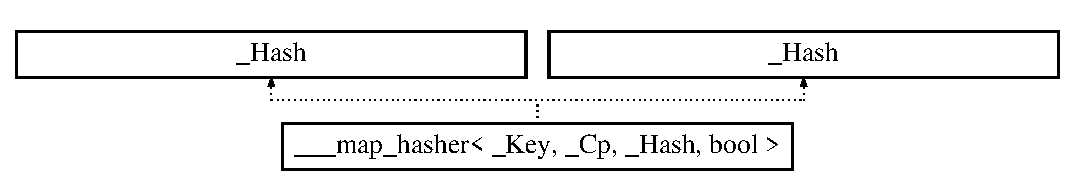
\includegraphics[height=2.000000cm]{class______map__hasher}
\end{center}
\end{figure}
\subsection*{Public Member Functions}
\begin{DoxyCompactItemize}
\item 
\+\_\+\+L\+I\+B\+C\+P\+P\+\_\+\+I\+N\+L\+I\+N\+E\+\_\+\+V\+I\+S\+I\+B\+I\+L\+I\+T\+Y \hyperlink{class______map__hasher_aaefe1bf01439916eaea11e4c6d7cd17b}{\+\_\+\+\_\+\+\_\+map\+\_\+hasher} () \+\_\+\+N\+O\+E\+X\+C\+E\+P\+T\+\_\+(is\+\_\+nothrow\+\_\+default\+\_\+constructible$<$ \+\_\+\+Hash $>$
\item 
\+\_\+\+L\+I\+B\+C\+P\+P\+\_\+\+I\+N\+L\+I\+N\+E\+\_\+\+V\+I\+S\+I\+B\+I\+L\+I\+T\+Y \hyperlink{class______map__hasher_ac4db69e3ab386b85e68bca517344fb2c}{\+\_\+\+\_\+\+\_\+map\+\_\+hasher} (const \+\_\+\+Hash \&\+\_\+\+\_\+h) \+\_\+\+N\+O\+E\+X\+C\+E\+P\+T\+\_\+(is\+\_\+nothrow\+\_\+copy\+\_\+constructible$<$ \+\_\+\+Hash $>$
\item 
\+\_\+\+L\+I\+B\+C\+P\+P\+\_\+\+I\+N\+L\+I\+N\+E\+\_\+\+V\+I\+S\+I\+B\+I\+L\+I\+T\+Y const \+\_\+\+Hash \& \hyperlink{class______map__hasher_a3bf000307ccac15d6fc1886aa5c390fd}{hash\+\_\+function} () const \+\_\+\+N\+O\+E\+X\+C\+E\+P\+T
\item 
\+\_\+\+L\+I\+B\+C\+P\+P\+\_\+\+I\+N\+L\+I\+N\+E\+\_\+\+V\+I\+S\+I\+B\+I\+L\+I\+T\+Y size\+\_\+t \hyperlink{class______map__hasher_a9536e86762187c3325bf995d816e17c5}{operator()} (const \+\_\+\+Cp \&\+\_\+\+\_\+x) const 
\item 
\+\_\+\+L\+I\+B\+C\+P\+P\+\_\+\+I\+N\+L\+I\+N\+E\+\_\+\+V\+I\+S\+I\+B\+I\+L\+I\+T\+Y size\+\_\+t \hyperlink{class______map__hasher_a38b257204597204eff179858e61a00d9}{operator()} (const \+\_\+\+Key \&\+\_\+\+\_\+x) const 
\item 
\+\_\+\+L\+I\+B\+C\+P\+P\+\_\+\+I\+N\+L\+I\+N\+E\+\_\+\+V\+I\+S\+I\+B\+I\+L\+I\+T\+Y \hyperlink{class______map__hasher_aaefe1bf01439916eaea11e4c6d7cd17b}{\+\_\+\+\_\+\+\_\+map\+\_\+hasher} () \+\_\+\+N\+O\+E\+X\+C\+E\+P\+T\+\_\+(is\+\_\+nothrow\+\_\+default\+\_\+constructible$<$ \+\_\+\+Hash $>$
\item 
\+\_\+\+L\+I\+B\+C\+P\+P\+\_\+\+I\+N\+L\+I\+N\+E\+\_\+\+V\+I\+S\+I\+B\+I\+L\+I\+T\+Y \hyperlink{class______map__hasher_ac4db69e3ab386b85e68bca517344fb2c}{\+\_\+\+\_\+\+\_\+map\+\_\+hasher} (const \+\_\+\+Hash \&\+\_\+\+\_\+h) \+\_\+\+N\+O\+E\+X\+C\+E\+P\+T\+\_\+(is\+\_\+nothrow\+\_\+copy\+\_\+constructible$<$ \+\_\+\+Hash $>$
\item 
\+\_\+\+L\+I\+B\+C\+P\+P\+\_\+\+I\+N\+L\+I\+N\+E\+\_\+\+V\+I\+S\+I\+B\+I\+L\+I\+T\+Y const \+\_\+\+Hash \& \hyperlink{class______map__hasher_a3bf000307ccac15d6fc1886aa5c390fd}{hash\+\_\+function} () const \+\_\+\+N\+O\+E\+X\+C\+E\+P\+T
\item 
\+\_\+\+L\+I\+B\+C\+P\+P\+\_\+\+I\+N\+L\+I\+N\+E\+\_\+\+V\+I\+S\+I\+B\+I\+L\+I\+T\+Y size\+\_\+t \hyperlink{class______map__hasher_a9536e86762187c3325bf995d816e17c5}{operator()} (const \+\_\+\+Cp \&\+\_\+\+\_\+x) const 
\item 
\+\_\+\+L\+I\+B\+C\+P\+P\+\_\+\+I\+N\+L\+I\+N\+E\+\_\+\+V\+I\+S\+I\+B\+I\+L\+I\+T\+Y size\+\_\+t \hyperlink{class______map__hasher_a38b257204597204eff179858e61a00d9}{operator()} (const \+\_\+\+Key \&\+\_\+\+\_\+x) const 
\end{DoxyCompactItemize}


\subsection{Detailed Description}
\subsubsection*{template$<$class \+\_\+\+Key, class \+\_\+\+Cp, class \+\_\+\+Hash, bool = is\+\_\+empty$<$\+\_\+\+Hash$>$\+::value$>$class \+\_\+\+\_\+\+\_\+map\+\_\+hasher$<$ \+\_\+\+Key, \+\_\+\+Cp, \+\_\+\+Hash, bool $>$}

is a scratch implementation of an unordered map class. 

\subsection{Constructor \& Destructor Documentation}
\hypertarget{class______map__hasher_aaefe1bf01439916eaea11e4c6d7cd17b}{}\index{\+\_\+\+\_\+\+\_\+map\+\_\+hasher@{\+\_\+\+\_\+\+\_\+map\+\_\+hasher}!\+\_\+\+\_\+\+\_\+map\+\_\+hasher@{\+\_\+\+\_\+\+\_\+map\+\_\+hasher}}
\index{\+\_\+\+\_\+\+\_\+map\+\_\+hasher@{\+\_\+\+\_\+\+\_\+map\+\_\+hasher}!\+\_\+\+\_\+\+\_\+map\+\_\+hasher@{\+\_\+\+\_\+\+\_\+map\+\_\+hasher}}
\subsubsection[{\+\_\+\+\_\+\+\_\+map\+\_\+hasher() \+\_\+\+N\+O\+E\+X\+C\+E\+P\+T\+\_\+(is\+\_\+nothrow\+\_\+default\+\_\+constructible$<$ \+\_\+\+Hash $>$}]{\setlength{\rightskip}{0pt plus 5cm}template$<$class \+\_\+\+Key , class \+\_\+\+Cp , class \+\_\+\+Hash , bool  = is\+\_\+empty$<$\+\_\+\+Hash$>$\+::value$>$ \+\_\+\+L\+I\+B\+C\+P\+P\+\_\+\+I\+N\+L\+I\+N\+E\+\_\+\+V\+I\+S\+I\+B\+I\+L\+I\+T\+Y {\bf \+\_\+\+\_\+\+\_\+map\+\_\+hasher}$<$ \+\_\+\+Key, \+\_\+\+Cp, \+\_\+\+Hash, bool $>$\+::{\bf \+\_\+\+\_\+\+\_\+map\+\_\+hasher} (
\begin{DoxyParamCaption}
{}
\end{DoxyParamCaption}
)\hspace{0.3cm}{\ttfamily [inline]}}\label{class______map__hasher_aaefe1bf01439916eaea11e4c6d7cd17b}
\hypertarget{class______map__hasher_ac4db69e3ab386b85e68bca517344fb2c}{}\index{\+\_\+\+\_\+\+\_\+map\+\_\+hasher@{\+\_\+\+\_\+\+\_\+map\+\_\+hasher}!\+\_\+\+\_\+\+\_\+map\+\_\+hasher@{\+\_\+\+\_\+\+\_\+map\+\_\+hasher}}
\index{\+\_\+\+\_\+\+\_\+map\+\_\+hasher@{\+\_\+\+\_\+\+\_\+map\+\_\+hasher}!\+\_\+\+\_\+\+\_\+map\+\_\+hasher@{\+\_\+\+\_\+\+\_\+map\+\_\+hasher}}
\subsubsection[{\+\_\+\+\_\+\+\_\+map\+\_\+hasher(const \+\_\+\+Hash \&\+\_\+\+\_\+h) \+\_\+\+N\+O\+E\+X\+C\+E\+P\+T\+\_\+(is\+\_\+nothrow\+\_\+copy\+\_\+constructible$<$ \+\_\+\+Hash $>$}]{\setlength{\rightskip}{0pt plus 5cm}template$<$class \+\_\+\+Key , class \+\_\+\+Cp , class \+\_\+\+Hash , bool  = is\+\_\+empty$<$\+\_\+\+Hash$>$\+::value$>$ \+\_\+\+L\+I\+B\+C\+P\+P\+\_\+\+I\+N\+L\+I\+N\+E\+\_\+\+V\+I\+S\+I\+B\+I\+L\+I\+T\+Y {\bf \+\_\+\+\_\+\+\_\+map\+\_\+hasher}$<$ \+\_\+\+Key, \+\_\+\+Cp, \+\_\+\+Hash, bool $>$\+::{\bf \+\_\+\+\_\+\+\_\+map\+\_\+hasher} (
\begin{DoxyParamCaption}
\item[{const \+\_\+\+Hash \&}]{\+\_\+\+\_\+h}
\end{DoxyParamCaption}
)\hspace{0.3cm}{\ttfamily [inline]}}\label{class______map__hasher_ac4db69e3ab386b85e68bca517344fb2c}
\hypertarget{class______map__hasher_aaefe1bf01439916eaea11e4c6d7cd17b}{}\index{\+\_\+\+\_\+\+\_\+map\+\_\+hasher@{\+\_\+\+\_\+\+\_\+map\+\_\+hasher}!\+\_\+\+\_\+\+\_\+map\+\_\+hasher@{\+\_\+\+\_\+\+\_\+map\+\_\+hasher}}
\index{\+\_\+\+\_\+\+\_\+map\+\_\+hasher@{\+\_\+\+\_\+\+\_\+map\+\_\+hasher}!\+\_\+\+\_\+\+\_\+map\+\_\+hasher@{\+\_\+\+\_\+\+\_\+map\+\_\+hasher}}
\subsubsection[{\+\_\+\+\_\+\+\_\+map\+\_\+hasher() \+\_\+\+N\+O\+E\+X\+C\+E\+P\+T\+\_\+(is\+\_\+nothrow\+\_\+default\+\_\+constructible$<$ \+\_\+\+Hash $>$}]{\setlength{\rightskip}{0pt plus 5cm}template$<$class \+\_\+\+Key , class \+\_\+\+Cp , class \+\_\+\+Hash , bool  = is\+\_\+empty$<$\+\_\+\+Hash$>$\+::value$>$ \+\_\+\+L\+I\+B\+C\+P\+P\+\_\+\+I\+N\+L\+I\+N\+E\+\_\+\+V\+I\+S\+I\+B\+I\+L\+I\+T\+Y {\bf \+\_\+\+\_\+\+\_\+map\+\_\+hasher}$<$ \+\_\+\+Key, \+\_\+\+Cp, \+\_\+\+Hash, bool $>$\+::{\bf \+\_\+\+\_\+\+\_\+map\+\_\+hasher} (
\begin{DoxyParamCaption}
{}
\end{DoxyParamCaption}
)\hspace{0.3cm}{\ttfamily [inline]}}\label{class______map__hasher_aaefe1bf01439916eaea11e4c6d7cd17b}
\hypertarget{class______map__hasher_ac4db69e3ab386b85e68bca517344fb2c}{}\index{\+\_\+\+\_\+\+\_\+map\+\_\+hasher@{\+\_\+\+\_\+\+\_\+map\+\_\+hasher}!\+\_\+\+\_\+\+\_\+map\+\_\+hasher@{\+\_\+\+\_\+\+\_\+map\+\_\+hasher}}
\index{\+\_\+\+\_\+\+\_\+map\+\_\+hasher@{\+\_\+\+\_\+\+\_\+map\+\_\+hasher}!\+\_\+\+\_\+\+\_\+map\+\_\+hasher@{\+\_\+\+\_\+\+\_\+map\+\_\+hasher}}
\subsubsection[{\+\_\+\+\_\+\+\_\+map\+\_\+hasher(const \+\_\+\+Hash \&\+\_\+\+\_\+h) \+\_\+\+N\+O\+E\+X\+C\+E\+P\+T\+\_\+(is\+\_\+nothrow\+\_\+copy\+\_\+constructible$<$ \+\_\+\+Hash $>$}]{\setlength{\rightskip}{0pt plus 5cm}template$<$class \+\_\+\+Key , class \+\_\+\+Cp , class \+\_\+\+Hash , bool  = is\+\_\+empty$<$\+\_\+\+Hash$>$\+::value$>$ \+\_\+\+L\+I\+B\+C\+P\+P\+\_\+\+I\+N\+L\+I\+N\+E\+\_\+\+V\+I\+S\+I\+B\+I\+L\+I\+T\+Y {\bf \+\_\+\+\_\+\+\_\+map\+\_\+hasher}$<$ \+\_\+\+Key, \+\_\+\+Cp, \+\_\+\+Hash, bool $>$\+::{\bf \+\_\+\+\_\+\+\_\+map\+\_\+hasher} (
\begin{DoxyParamCaption}
\item[{const \+\_\+\+Hash \&}]{\+\_\+\+\_\+h}
\end{DoxyParamCaption}
)\hspace{0.3cm}{\ttfamily [inline]}}\label{class______map__hasher_ac4db69e3ab386b85e68bca517344fb2c}


\subsection{Member Function Documentation}
\hypertarget{class______map__hasher_a3bf000307ccac15d6fc1886aa5c390fd}{}\index{\+\_\+\+\_\+\+\_\+map\+\_\+hasher@{\+\_\+\+\_\+\+\_\+map\+\_\+hasher}!hash\+\_\+function@{hash\+\_\+function}}
\index{hash\+\_\+function@{hash\+\_\+function}!\+\_\+\+\_\+\+\_\+map\+\_\+hasher@{\+\_\+\+\_\+\+\_\+map\+\_\+hasher}}
\subsubsection[{hash\+\_\+function() const \+\_\+\+N\+O\+E\+X\+C\+E\+P\+T}]{\setlength{\rightskip}{0pt plus 5cm}template$<$class \+\_\+\+Key , class \+\_\+\+Cp , class \+\_\+\+Hash , bool  = is\+\_\+empty$<$\+\_\+\+Hash$>$\+::value$>$ \+\_\+\+L\+I\+B\+C\+P\+P\+\_\+\+I\+N\+L\+I\+N\+E\+\_\+\+V\+I\+S\+I\+B\+I\+L\+I\+T\+Y const \+\_\+\+Hash\& {\bf \+\_\+\+\_\+\+\_\+map\+\_\+hasher}$<$ \+\_\+\+Key, \+\_\+\+Cp, \+\_\+\+Hash, bool $>$\+::hash\+\_\+function (
\begin{DoxyParamCaption}
{}
\end{DoxyParamCaption}
) const\hspace{0.3cm}{\ttfamily [inline]}}\label{class______map__hasher_a3bf000307ccac15d6fc1886aa5c390fd}
\hypertarget{class______map__hasher_a3bf000307ccac15d6fc1886aa5c390fd}{}\index{\+\_\+\+\_\+\+\_\+map\+\_\+hasher@{\+\_\+\+\_\+\+\_\+map\+\_\+hasher}!hash\+\_\+function@{hash\+\_\+function}}
\index{hash\+\_\+function@{hash\+\_\+function}!\+\_\+\+\_\+\+\_\+map\+\_\+hasher@{\+\_\+\+\_\+\+\_\+map\+\_\+hasher}}
\subsubsection[{hash\+\_\+function() const \+\_\+\+N\+O\+E\+X\+C\+E\+P\+T}]{\setlength{\rightskip}{0pt plus 5cm}template$<$class \+\_\+\+Key , class \+\_\+\+Cp , class \+\_\+\+Hash , bool  = is\+\_\+empty$<$\+\_\+\+Hash$>$\+::value$>$ \+\_\+\+L\+I\+B\+C\+P\+P\+\_\+\+I\+N\+L\+I\+N\+E\+\_\+\+V\+I\+S\+I\+B\+I\+L\+I\+T\+Y const \+\_\+\+Hash\& {\bf \+\_\+\+\_\+\+\_\+map\+\_\+hasher}$<$ \+\_\+\+Key, \+\_\+\+Cp, \+\_\+\+Hash, bool $>$\+::hash\+\_\+function (
\begin{DoxyParamCaption}
{}
\end{DoxyParamCaption}
) const\hspace{0.3cm}{\ttfamily [inline]}}\label{class______map__hasher_a3bf000307ccac15d6fc1886aa5c390fd}
\hypertarget{class______map__hasher_a9536e86762187c3325bf995d816e17c5}{}\index{\+\_\+\+\_\+\+\_\+map\+\_\+hasher@{\+\_\+\+\_\+\+\_\+map\+\_\+hasher}!operator()@{operator()}}
\index{operator()@{operator()}!\+\_\+\+\_\+\+\_\+map\+\_\+hasher@{\+\_\+\+\_\+\+\_\+map\+\_\+hasher}}
\subsubsection[{operator()(const \+\_\+\+Cp \&\+\_\+\+\_\+x) const }]{\setlength{\rightskip}{0pt plus 5cm}template$<$class \+\_\+\+Key , class \+\_\+\+Cp , class \+\_\+\+Hash , bool  = is\+\_\+empty$<$\+\_\+\+Hash$>$\+::value$>$ \+\_\+\+L\+I\+B\+C\+P\+P\+\_\+\+I\+N\+L\+I\+N\+E\+\_\+\+V\+I\+S\+I\+B\+I\+L\+I\+T\+Y size\+\_\+t {\bf \+\_\+\+\_\+\+\_\+map\+\_\+hasher}$<$ \+\_\+\+Key, \+\_\+\+Cp, \+\_\+\+Hash, bool $>$\+::operator() (
\begin{DoxyParamCaption}
\item[{const \+\_\+\+Cp \&}]{\+\_\+\+\_\+x}
\end{DoxyParamCaption}
) const\hspace{0.3cm}{\ttfamily [inline]}}\label{class______map__hasher_a9536e86762187c3325bf995d816e17c5}
\hypertarget{class______map__hasher_a9536e86762187c3325bf995d816e17c5}{}\index{\+\_\+\+\_\+\+\_\+map\+\_\+hasher@{\+\_\+\+\_\+\+\_\+map\+\_\+hasher}!operator()@{operator()}}
\index{operator()@{operator()}!\+\_\+\+\_\+\+\_\+map\+\_\+hasher@{\+\_\+\+\_\+\+\_\+map\+\_\+hasher}}
\subsubsection[{operator()(const \+\_\+\+Cp \&\+\_\+\+\_\+x) const }]{\setlength{\rightskip}{0pt plus 5cm}template$<$class \+\_\+\+Key , class \+\_\+\+Cp , class \+\_\+\+Hash , bool  = is\+\_\+empty$<$\+\_\+\+Hash$>$\+::value$>$ \+\_\+\+L\+I\+B\+C\+P\+P\+\_\+\+I\+N\+L\+I\+N\+E\+\_\+\+V\+I\+S\+I\+B\+I\+L\+I\+T\+Y size\+\_\+t {\bf \+\_\+\+\_\+\+\_\+map\+\_\+hasher}$<$ \+\_\+\+Key, \+\_\+\+Cp, \+\_\+\+Hash, bool $>$\+::operator() (
\begin{DoxyParamCaption}
\item[{const \+\_\+\+Cp \&}]{\+\_\+\+\_\+x}
\end{DoxyParamCaption}
) const\hspace{0.3cm}{\ttfamily [inline]}}\label{class______map__hasher_a9536e86762187c3325bf995d816e17c5}
\hypertarget{class______map__hasher_a38b257204597204eff179858e61a00d9}{}\index{\+\_\+\+\_\+\+\_\+map\+\_\+hasher@{\+\_\+\+\_\+\+\_\+map\+\_\+hasher}!operator()@{operator()}}
\index{operator()@{operator()}!\+\_\+\+\_\+\+\_\+map\+\_\+hasher@{\+\_\+\+\_\+\+\_\+map\+\_\+hasher}}
\subsubsection[{operator()(const \+\_\+\+Key \&\+\_\+\+\_\+x) const }]{\setlength{\rightskip}{0pt plus 5cm}template$<$class \+\_\+\+Key , class \+\_\+\+Cp , class \+\_\+\+Hash , bool  = is\+\_\+empty$<$\+\_\+\+Hash$>$\+::value$>$ \+\_\+\+L\+I\+B\+C\+P\+P\+\_\+\+I\+N\+L\+I\+N\+E\+\_\+\+V\+I\+S\+I\+B\+I\+L\+I\+T\+Y size\+\_\+t {\bf \+\_\+\+\_\+\+\_\+map\+\_\+hasher}$<$ \+\_\+\+Key, \+\_\+\+Cp, \+\_\+\+Hash, bool $>$\+::operator() (
\begin{DoxyParamCaption}
\item[{const \+\_\+\+Key \&}]{\+\_\+\+\_\+x}
\end{DoxyParamCaption}
) const\hspace{0.3cm}{\ttfamily [inline]}}\label{class______map__hasher_a38b257204597204eff179858e61a00d9}
\hypertarget{class______map__hasher_a38b257204597204eff179858e61a00d9}{}\index{\+\_\+\+\_\+\+\_\+map\+\_\+hasher@{\+\_\+\+\_\+\+\_\+map\+\_\+hasher}!operator()@{operator()}}
\index{operator()@{operator()}!\+\_\+\+\_\+\+\_\+map\+\_\+hasher@{\+\_\+\+\_\+\+\_\+map\+\_\+hasher}}
\subsubsection[{operator()(const \+\_\+\+Key \&\+\_\+\+\_\+x) const }]{\setlength{\rightskip}{0pt plus 5cm}template$<$class \+\_\+\+Key , class \+\_\+\+Cp , class \+\_\+\+Hash , bool  = is\+\_\+empty$<$\+\_\+\+Hash$>$\+::value$>$ \+\_\+\+L\+I\+B\+C\+P\+P\+\_\+\+I\+N\+L\+I\+N\+E\+\_\+\+V\+I\+S\+I\+B\+I\+L\+I\+T\+Y size\+\_\+t {\bf \+\_\+\+\_\+\+\_\+map\+\_\+hasher}$<$ \+\_\+\+Key, \+\_\+\+Cp, \+\_\+\+Hash, bool $>$\+::operator() (
\begin{DoxyParamCaption}
\item[{const \+\_\+\+Key \&}]{\+\_\+\+\_\+x}
\end{DoxyParamCaption}
) const\hspace{0.3cm}{\ttfamily [inline]}}\label{class______map__hasher_a38b257204597204eff179858e61a00d9}


The documentation for this class was generated from the following files\+:\begin{DoxyCompactItemize}
\item 
/\+Users/brandonmcfarland/\+Desktop/searchdocs/\+Search\+Engine/\+Final\+Project/\hyperlink{mapping_8cpp}{mapping.\+cpp}\item 
/\+Users/brandonmcfarland/\+Desktop/searchdocs/\+Search\+Engine/\+Final\+Project/\hyperlink{mapping_8h}{mapping.\+h}\end{DoxyCompactItemize}

\hypertarget{class______map__hasher_3_01___key_00_01___cp_00_01___hash_00_01false_01_4}{}\section{\+\_\+\+\_\+\+\_\+map\+\_\+hasher$<$ \+\_\+\+Key, \+\_\+\+Cp, \+\_\+\+Hash, false $>$ Class Template Reference}
\label{class______map__hasher_3_01___key_00_01___cp_00_01___hash_00_01false_01_4}\index{\+\_\+\+\_\+\+\_\+map\+\_\+hasher$<$ \+\_\+\+Key, \+\_\+\+Cp, \+\_\+\+Hash, false $>$@{\+\_\+\+\_\+\+\_\+map\+\_\+hasher$<$ \+\_\+\+Key, \+\_\+\+Cp, \+\_\+\+Hash, false $>$}}


{\ttfamily \#include $<$mapping.\+h$>$}

\subsection*{Public Member Functions}
\begin{DoxyCompactItemize}
\item 
\+\_\+\+L\+I\+B\+C\+P\+P\+\_\+\+I\+N\+L\+I\+N\+E\+\_\+\+V\+I\+S\+I\+B\+I\+L\+I\+T\+Y \hyperlink{class______map__hasher_3_01___key_00_01___cp_00_01___hash_00_01false_01_4_ae1078b1247c357a13a8d2f6ef1ec4399}{\+\_\+\+\_\+\+\_\+map\+\_\+hasher} () \+\_\+\+N\+O\+E\+X\+C\+E\+P\+T\+\_\+(is\+\_\+nothrow\+\_\+default\+\_\+constructible$<$ \+\_\+\+Hash $>$
\item 
\+\_\+\+L\+I\+B\+C\+P\+P\+\_\+\+I\+N\+L\+I\+N\+E\+\_\+\+V\+I\+S\+I\+B\+I\+L\+I\+T\+Y \hyperlink{class______map__hasher_3_01___key_00_01___cp_00_01___hash_00_01false_01_4_a76cca625eb676b114276721b9818cc0b}{\+\_\+\+\_\+\+\_\+map\+\_\+hasher} (const \+\_\+\+Hash \&\+\_\+\+\_\+h) \+\_\+\+N\+O\+E\+X\+C\+E\+P\+T\+\_\+(is\+\_\+nothrow\+\_\+copy\+\_\+constructible$<$ \+\_\+\+Hash $>$
\item 
\+\_\+\+L\+I\+B\+C\+P\+P\+\_\+\+I\+N\+L\+I\+N\+E\+\_\+\+V\+I\+S\+I\+B\+I\+L\+I\+T\+Y const \+\_\+\+Hash \& \hyperlink{class______map__hasher_3_01___key_00_01___cp_00_01___hash_00_01false_01_4_a36b4694cf944a1a28969d3f6917cc9a9}{hash\+\_\+function} () const \+\_\+\+N\+O\+E\+X\+C\+E\+P\+T
\item 
\+\_\+\+L\+I\+B\+C\+P\+P\+\_\+\+I\+N\+L\+I\+N\+E\+\_\+\+V\+I\+S\+I\+B\+I\+L\+I\+T\+Y size\+\_\+t \hyperlink{class______map__hasher_3_01___key_00_01___cp_00_01___hash_00_01false_01_4_a4320bf7187c7c20511393415142a3651}{operator()} (const \+\_\+\+Cp \&\+\_\+\+\_\+x) const 
\item 
\+\_\+\+L\+I\+B\+C\+P\+P\+\_\+\+I\+N\+L\+I\+N\+E\+\_\+\+V\+I\+S\+I\+B\+I\+L\+I\+T\+Y size\+\_\+t \hyperlink{class______map__hasher_3_01___key_00_01___cp_00_01___hash_00_01false_01_4_a81e792db8b661f6bbd204d69ffe6eb86}{operator()} (const \+\_\+\+Key \&\+\_\+\+\_\+x) const 
\item 
\+\_\+\+L\+I\+B\+C\+P\+P\+\_\+\+I\+N\+L\+I\+N\+E\+\_\+\+V\+I\+S\+I\+B\+I\+L\+I\+T\+Y \hyperlink{class______map__hasher_3_01___key_00_01___cp_00_01___hash_00_01false_01_4_ae1078b1247c357a13a8d2f6ef1ec4399}{\+\_\+\+\_\+\+\_\+map\+\_\+hasher} () \+\_\+\+N\+O\+E\+X\+C\+E\+P\+T\+\_\+(is\+\_\+nothrow\+\_\+default\+\_\+constructible$<$ \+\_\+\+Hash $>$
\item 
\+\_\+\+L\+I\+B\+C\+P\+P\+\_\+\+I\+N\+L\+I\+N\+E\+\_\+\+V\+I\+S\+I\+B\+I\+L\+I\+T\+Y \hyperlink{class______map__hasher_3_01___key_00_01___cp_00_01___hash_00_01false_01_4_a76cca625eb676b114276721b9818cc0b}{\+\_\+\+\_\+\+\_\+map\+\_\+hasher} (const \+\_\+\+Hash \&\+\_\+\+\_\+h) \+\_\+\+N\+O\+E\+X\+C\+E\+P\+T\+\_\+(is\+\_\+nothrow\+\_\+copy\+\_\+constructible$<$ \+\_\+\+Hash $>$
\item 
\+\_\+\+L\+I\+B\+C\+P\+P\+\_\+\+I\+N\+L\+I\+N\+E\+\_\+\+V\+I\+S\+I\+B\+I\+L\+I\+T\+Y const \+\_\+\+Hash \& \hyperlink{class______map__hasher_3_01___key_00_01___cp_00_01___hash_00_01false_01_4_a36b4694cf944a1a28969d3f6917cc9a9}{hash\+\_\+function} () const \+\_\+\+N\+O\+E\+X\+C\+E\+P\+T
\item 
\+\_\+\+L\+I\+B\+C\+P\+P\+\_\+\+I\+N\+L\+I\+N\+E\+\_\+\+V\+I\+S\+I\+B\+I\+L\+I\+T\+Y size\+\_\+t \hyperlink{class______map__hasher_3_01___key_00_01___cp_00_01___hash_00_01false_01_4_a4320bf7187c7c20511393415142a3651}{operator()} (const \+\_\+\+Cp \&\+\_\+\+\_\+x) const 
\item 
\+\_\+\+L\+I\+B\+C\+P\+P\+\_\+\+I\+N\+L\+I\+N\+E\+\_\+\+V\+I\+S\+I\+B\+I\+L\+I\+T\+Y size\+\_\+t \hyperlink{class______map__hasher_3_01___key_00_01___cp_00_01___hash_00_01false_01_4_a81e792db8b661f6bbd204d69ffe6eb86}{operator()} (const \+\_\+\+Key \&\+\_\+\+\_\+x) const 
\end{DoxyCompactItemize}


\subsection{Constructor \& Destructor Documentation}
\hypertarget{class______map__hasher_3_01___key_00_01___cp_00_01___hash_00_01false_01_4_ae1078b1247c357a13a8d2f6ef1ec4399}{}\index{\+\_\+\+\_\+\+\_\+map\+\_\+hasher$<$ \+\_\+\+Key, \+\_\+\+Cp, \+\_\+\+Hash, false $>$@{\+\_\+\+\_\+\+\_\+map\+\_\+hasher$<$ \+\_\+\+Key, \+\_\+\+Cp, \+\_\+\+Hash, false $>$}!\+\_\+\+\_\+\+\_\+map\+\_\+hasher@{\+\_\+\+\_\+\+\_\+map\+\_\+hasher}}
\index{\+\_\+\+\_\+\+\_\+map\+\_\+hasher@{\+\_\+\+\_\+\+\_\+map\+\_\+hasher}!\+\_\+\+\_\+\+\_\+map\+\_\+hasher$<$ \+\_\+\+Key, \+\_\+\+Cp, \+\_\+\+Hash, false $>$@{\+\_\+\+\_\+\+\_\+map\+\_\+hasher$<$ \+\_\+\+Key, \+\_\+\+Cp, \+\_\+\+Hash, false $>$}}
\subsubsection[{\+\_\+\+\_\+\+\_\+map\+\_\+hasher() \+\_\+\+N\+O\+E\+X\+C\+E\+P\+T\+\_\+(is\+\_\+nothrow\+\_\+default\+\_\+constructible$<$ \+\_\+\+Hash $>$}]{\setlength{\rightskip}{0pt plus 5cm}template$<$class \+\_\+\+Key , class \+\_\+\+Cp , class \+\_\+\+Hash $>$ \+\_\+\+L\+I\+B\+C\+P\+P\+\_\+\+I\+N\+L\+I\+N\+E\+\_\+\+V\+I\+S\+I\+B\+I\+L\+I\+T\+Y {\bf \+\_\+\+\_\+\+\_\+map\+\_\+hasher}$<$ \+\_\+\+Key, \+\_\+\+Cp, \+\_\+\+Hash, false $>$\+::{\bf \+\_\+\+\_\+\+\_\+map\+\_\+hasher} (
\begin{DoxyParamCaption}
{}
\end{DoxyParamCaption}
)\hspace{0.3cm}{\ttfamily [inline]}}\label{class______map__hasher_3_01___key_00_01___cp_00_01___hash_00_01false_01_4_ae1078b1247c357a13a8d2f6ef1ec4399}
\hypertarget{class______map__hasher_3_01___key_00_01___cp_00_01___hash_00_01false_01_4_a76cca625eb676b114276721b9818cc0b}{}\index{\+\_\+\+\_\+\+\_\+map\+\_\+hasher$<$ \+\_\+\+Key, \+\_\+\+Cp, \+\_\+\+Hash, false $>$@{\+\_\+\+\_\+\+\_\+map\+\_\+hasher$<$ \+\_\+\+Key, \+\_\+\+Cp, \+\_\+\+Hash, false $>$}!\+\_\+\+\_\+\+\_\+map\+\_\+hasher@{\+\_\+\+\_\+\+\_\+map\+\_\+hasher}}
\index{\+\_\+\+\_\+\+\_\+map\+\_\+hasher@{\+\_\+\+\_\+\+\_\+map\+\_\+hasher}!\+\_\+\+\_\+\+\_\+map\+\_\+hasher$<$ \+\_\+\+Key, \+\_\+\+Cp, \+\_\+\+Hash, false $>$@{\+\_\+\+\_\+\+\_\+map\+\_\+hasher$<$ \+\_\+\+Key, \+\_\+\+Cp, \+\_\+\+Hash, false $>$}}
\subsubsection[{\+\_\+\+\_\+\+\_\+map\+\_\+hasher(const \+\_\+\+Hash \&\+\_\+\+\_\+h) \+\_\+\+N\+O\+E\+X\+C\+E\+P\+T\+\_\+(is\+\_\+nothrow\+\_\+copy\+\_\+constructible$<$ \+\_\+\+Hash $>$}]{\setlength{\rightskip}{0pt plus 5cm}template$<$class \+\_\+\+Key , class \+\_\+\+Cp , class \+\_\+\+Hash $>$ \+\_\+\+L\+I\+B\+C\+P\+P\+\_\+\+I\+N\+L\+I\+N\+E\+\_\+\+V\+I\+S\+I\+B\+I\+L\+I\+T\+Y {\bf \+\_\+\+\_\+\+\_\+map\+\_\+hasher}$<$ \+\_\+\+Key, \+\_\+\+Cp, \+\_\+\+Hash, false $>$\+::{\bf \+\_\+\+\_\+\+\_\+map\+\_\+hasher} (
\begin{DoxyParamCaption}
\item[{const \+\_\+\+Hash \&}]{\+\_\+\+\_\+h}
\end{DoxyParamCaption}
)\hspace{0.3cm}{\ttfamily [inline]}}\label{class______map__hasher_3_01___key_00_01___cp_00_01___hash_00_01false_01_4_a76cca625eb676b114276721b9818cc0b}
\hypertarget{class______map__hasher_3_01___key_00_01___cp_00_01___hash_00_01false_01_4_ae1078b1247c357a13a8d2f6ef1ec4399}{}\index{\+\_\+\+\_\+\+\_\+map\+\_\+hasher$<$ \+\_\+\+Key, \+\_\+\+Cp, \+\_\+\+Hash, false $>$@{\+\_\+\+\_\+\+\_\+map\+\_\+hasher$<$ \+\_\+\+Key, \+\_\+\+Cp, \+\_\+\+Hash, false $>$}!\+\_\+\+\_\+\+\_\+map\+\_\+hasher@{\+\_\+\+\_\+\+\_\+map\+\_\+hasher}}
\index{\+\_\+\+\_\+\+\_\+map\+\_\+hasher@{\+\_\+\+\_\+\+\_\+map\+\_\+hasher}!\+\_\+\+\_\+\+\_\+map\+\_\+hasher$<$ \+\_\+\+Key, \+\_\+\+Cp, \+\_\+\+Hash, false $>$@{\+\_\+\+\_\+\+\_\+map\+\_\+hasher$<$ \+\_\+\+Key, \+\_\+\+Cp, \+\_\+\+Hash, false $>$}}
\subsubsection[{\+\_\+\+\_\+\+\_\+map\+\_\+hasher() \+\_\+\+N\+O\+E\+X\+C\+E\+P\+T\+\_\+(is\+\_\+nothrow\+\_\+default\+\_\+constructible$<$ \+\_\+\+Hash $>$}]{\setlength{\rightskip}{0pt plus 5cm}template$<$class \+\_\+\+Key , class \+\_\+\+Cp , class \+\_\+\+Hash $>$ \+\_\+\+L\+I\+B\+C\+P\+P\+\_\+\+I\+N\+L\+I\+N\+E\+\_\+\+V\+I\+S\+I\+B\+I\+L\+I\+T\+Y {\bf \+\_\+\+\_\+\+\_\+map\+\_\+hasher}$<$ \+\_\+\+Key, \+\_\+\+Cp, \+\_\+\+Hash, false $>$\+::{\bf \+\_\+\+\_\+\+\_\+map\+\_\+hasher} (
\begin{DoxyParamCaption}
{}
\end{DoxyParamCaption}
)\hspace{0.3cm}{\ttfamily [inline]}}\label{class______map__hasher_3_01___key_00_01___cp_00_01___hash_00_01false_01_4_ae1078b1247c357a13a8d2f6ef1ec4399}
\hypertarget{class______map__hasher_3_01___key_00_01___cp_00_01___hash_00_01false_01_4_a76cca625eb676b114276721b9818cc0b}{}\index{\+\_\+\+\_\+\+\_\+map\+\_\+hasher$<$ \+\_\+\+Key, \+\_\+\+Cp, \+\_\+\+Hash, false $>$@{\+\_\+\+\_\+\+\_\+map\+\_\+hasher$<$ \+\_\+\+Key, \+\_\+\+Cp, \+\_\+\+Hash, false $>$}!\+\_\+\+\_\+\+\_\+map\+\_\+hasher@{\+\_\+\+\_\+\+\_\+map\+\_\+hasher}}
\index{\+\_\+\+\_\+\+\_\+map\+\_\+hasher@{\+\_\+\+\_\+\+\_\+map\+\_\+hasher}!\+\_\+\+\_\+\+\_\+map\+\_\+hasher$<$ \+\_\+\+Key, \+\_\+\+Cp, \+\_\+\+Hash, false $>$@{\+\_\+\+\_\+\+\_\+map\+\_\+hasher$<$ \+\_\+\+Key, \+\_\+\+Cp, \+\_\+\+Hash, false $>$}}
\subsubsection[{\+\_\+\+\_\+\+\_\+map\+\_\+hasher(const \+\_\+\+Hash \&\+\_\+\+\_\+h) \+\_\+\+N\+O\+E\+X\+C\+E\+P\+T\+\_\+(is\+\_\+nothrow\+\_\+copy\+\_\+constructible$<$ \+\_\+\+Hash $>$}]{\setlength{\rightskip}{0pt plus 5cm}template$<$class \+\_\+\+Key , class \+\_\+\+Cp , class \+\_\+\+Hash $>$ \+\_\+\+L\+I\+B\+C\+P\+P\+\_\+\+I\+N\+L\+I\+N\+E\+\_\+\+V\+I\+S\+I\+B\+I\+L\+I\+T\+Y {\bf \+\_\+\+\_\+\+\_\+map\+\_\+hasher}$<$ \+\_\+\+Key, \+\_\+\+Cp, \+\_\+\+Hash, false $>$\+::{\bf \+\_\+\+\_\+\+\_\+map\+\_\+hasher} (
\begin{DoxyParamCaption}
\item[{const \+\_\+\+Hash \&}]{\+\_\+\+\_\+h}
\end{DoxyParamCaption}
)\hspace{0.3cm}{\ttfamily [inline]}}\label{class______map__hasher_3_01___key_00_01___cp_00_01___hash_00_01false_01_4_a76cca625eb676b114276721b9818cc0b}


\subsection{Member Function Documentation}
\hypertarget{class______map__hasher_3_01___key_00_01___cp_00_01___hash_00_01false_01_4_a36b4694cf944a1a28969d3f6917cc9a9}{}\index{\+\_\+\+\_\+\+\_\+map\+\_\+hasher$<$ \+\_\+\+Key, \+\_\+\+Cp, \+\_\+\+Hash, false $>$@{\+\_\+\+\_\+\+\_\+map\+\_\+hasher$<$ \+\_\+\+Key, \+\_\+\+Cp, \+\_\+\+Hash, false $>$}!hash\+\_\+function@{hash\+\_\+function}}
\index{hash\+\_\+function@{hash\+\_\+function}!\+\_\+\+\_\+\+\_\+map\+\_\+hasher$<$ \+\_\+\+Key, \+\_\+\+Cp, \+\_\+\+Hash, false $>$@{\+\_\+\+\_\+\+\_\+map\+\_\+hasher$<$ \+\_\+\+Key, \+\_\+\+Cp, \+\_\+\+Hash, false $>$}}
\subsubsection[{hash\+\_\+function() const \+\_\+\+N\+O\+E\+X\+C\+E\+P\+T}]{\setlength{\rightskip}{0pt plus 5cm}template$<$class \+\_\+\+Key , class \+\_\+\+Cp , class \+\_\+\+Hash $>$ \+\_\+\+L\+I\+B\+C\+P\+P\+\_\+\+I\+N\+L\+I\+N\+E\+\_\+\+V\+I\+S\+I\+B\+I\+L\+I\+T\+Y const \+\_\+\+Hash\& {\bf \+\_\+\+\_\+\+\_\+map\+\_\+hasher}$<$ \+\_\+\+Key, \+\_\+\+Cp, \+\_\+\+Hash, false $>$\+::hash\+\_\+function (
\begin{DoxyParamCaption}
{}
\end{DoxyParamCaption}
) const\hspace{0.3cm}{\ttfamily [inline]}}\label{class______map__hasher_3_01___key_00_01___cp_00_01___hash_00_01false_01_4_a36b4694cf944a1a28969d3f6917cc9a9}
\hypertarget{class______map__hasher_3_01___key_00_01___cp_00_01___hash_00_01false_01_4_a36b4694cf944a1a28969d3f6917cc9a9}{}\index{\+\_\+\+\_\+\+\_\+map\+\_\+hasher$<$ \+\_\+\+Key, \+\_\+\+Cp, \+\_\+\+Hash, false $>$@{\+\_\+\+\_\+\+\_\+map\+\_\+hasher$<$ \+\_\+\+Key, \+\_\+\+Cp, \+\_\+\+Hash, false $>$}!hash\+\_\+function@{hash\+\_\+function}}
\index{hash\+\_\+function@{hash\+\_\+function}!\+\_\+\+\_\+\+\_\+map\+\_\+hasher$<$ \+\_\+\+Key, \+\_\+\+Cp, \+\_\+\+Hash, false $>$@{\+\_\+\+\_\+\+\_\+map\+\_\+hasher$<$ \+\_\+\+Key, \+\_\+\+Cp, \+\_\+\+Hash, false $>$}}
\subsubsection[{hash\+\_\+function() const \+\_\+\+N\+O\+E\+X\+C\+E\+P\+T}]{\setlength{\rightskip}{0pt plus 5cm}template$<$class \+\_\+\+Key , class \+\_\+\+Cp , class \+\_\+\+Hash $>$ \+\_\+\+L\+I\+B\+C\+P\+P\+\_\+\+I\+N\+L\+I\+N\+E\+\_\+\+V\+I\+S\+I\+B\+I\+L\+I\+T\+Y const \+\_\+\+Hash\& {\bf \+\_\+\+\_\+\+\_\+map\+\_\+hasher}$<$ \+\_\+\+Key, \+\_\+\+Cp, \+\_\+\+Hash, false $>$\+::hash\+\_\+function (
\begin{DoxyParamCaption}
{}
\end{DoxyParamCaption}
) const\hspace{0.3cm}{\ttfamily [inline]}}\label{class______map__hasher_3_01___key_00_01___cp_00_01___hash_00_01false_01_4_a36b4694cf944a1a28969d3f6917cc9a9}
\hypertarget{class______map__hasher_3_01___key_00_01___cp_00_01___hash_00_01false_01_4_a4320bf7187c7c20511393415142a3651}{}\index{\+\_\+\+\_\+\+\_\+map\+\_\+hasher$<$ \+\_\+\+Key, \+\_\+\+Cp, \+\_\+\+Hash, false $>$@{\+\_\+\+\_\+\+\_\+map\+\_\+hasher$<$ \+\_\+\+Key, \+\_\+\+Cp, \+\_\+\+Hash, false $>$}!operator()@{operator()}}
\index{operator()@{operator()}!\+\_\+\+\_\+\+\_\+map\+\_\+hasher$<$ \+\_\+\+Key, \+\_\+\+Cp, \+\_\+\+Hash, false $>$@{\+\_\+\+\_\+\+\_\+map\+\_\+hasher$<$ \+\_\+\+Key, \+\_\+\+Cp, \+\_\+\+Hash, false $>$}}
\subsubsection[{operator()(const \+\_\+\+Cp \&\+\_\+\+\_\+x) const }]{\setlength{\rightskip}{0pt plus 5cm}template$<$class \+\_\+\+Key , class \+\_\+\+Cp , class \+\_\+\+Hash $>$ \+\_\+\+L\+I\+B\+C\+P\+P\+\_\+\+I\+N\+L\+I\+N\+E\+\_\+\+V\+I\+S\+I\+B\+I\+L\+I\+T\+Y size\+\_\+t {\bf \+\_\+\+\_\+\+\_\+map\+\_\+hasher}$<$ \+\_\+\+Key, \+\_\+\+Cp, \+\_\+\+Hash, false $>$\+::operator() (
\begin{DoxyParamCaption}
\item[{const \+\_\+\+Cp \&}]{\+\_\+\+\_\+x}
\end{DoxyParamCaption}
) const\hspace{0.3cm}{\ttfamily [inline]}}\label{class______map__hasher_3_01___key_00_01___cp_00_01___hash_00_01false_01_4_a4320bf7187c7c20511393415142a3651}
\hypertarget{class______map__hasher_3_01___key_00_01___cp_00_01___hash_00_01false_01_4_a4320bf7187c7c20511393415142a3651}{}\index{\+\_\+\+\_\+\+\_\+map\+\_\+hasher$<$ \+\_\+\+Key, \+\_\+\+Cp, \+\_\+\+Hash, false $>$@{\+\_\+\+\_\+\+\_\+map\+\_\+hasher$<$ \+\_\+\+Key, \+\_\+\+Cp, \+\_\+\+Hash, false $>$}!operator()@{operator()}}
\index{operator()@{operator()}!\+\_\+\+\_\+\+\_\+map\+\_\+hasher$<$ \+\_\+\+Key, \+\_\+\+Cp, \+\_\+\+Hash, false $>$@{\+\_\+\+\_\+\+\_\+map\+\_\+hasher$<$ \+\_\+\+Key, \+\_\+\+Cp, \+\_\+\+Hash, false $>$}}
\subsubsection[{operator()(const \+\_\+\+Cp \&\+\_\+\+\_\+x) const }]{\setlength{\rightskip}{0pt plus 5cm}template$<$class \+\_\+\+Key , class \+\_\+\+Cp , class \+\_\+\+Hash $>$ \+\_\+\+L\+I\+B\+C\+P\+P\+\_\+\+I\+N\+L\+I\+N\+E\+\_\+\+V\+I\+S\+I\+B\+I\+L\+I\+T\+Y size\+\_\+t {\bf \+\_\+\+\_\+\+\_\+map\+\_\+hasher}$<$ \+\_\+\+Key, \+\_\+\+Cp, \+\_\+\+Hash, false $>$\+::operator() (
\begin{DoxyParamCaption}
\item[{const \+\_\+\+Cp \&}]{\+\_\+\+\_\+x}
\end{DoxyParamCaption}
) const\hspace{0.3cm}{\ttfamily [inline]}}\label{class______map__hasher_3_01___key_00_01___cp_00_01___hash_00_01false_01_4_a4320bf7187c7c20511393415142a3651}
\hypertarget{class______map__hasher_3_01___key_00_01___cp_00_01___hash_00_01false_01_4_a81e792db8b661f6bbd204d69ffe6eb86}{}\index{\+\_\+\+\_\+\+\_\+map\+\_\+hasher$<$ \+\_\+\+Key, \+\_\+\+Cp, \+\_\+\+Hash, false $>$@{\+\_\+\+\_\+\+\_\+map\+\_\+hasher$<$ \+\_\+\+Key, \+\_\+\+Cp, \+\_\+\+Hash, false $>$}!operator()@{operator()}}
\index{operator()@{operator()}!\+\_\+\+\_\+\+\_\+map\+\_\+hasher$<$ \+\_\+\+Key, \+\_\+\+Cp, \+\_\+\+Hash, false $>$@{\+\_\+\+\_\+\+\_\+map\+\_\+hasher$<$ \+\_\+\+Key, \+\_\+\+Cp, \+\_\+\+Hash, false $>$}}
\subsubsection[{operator()(const \+\_\+\+Key \&\+\_\+\+\_\+x) const }]{\setlength{\rightskip}{0pt plus 5cm}template$<$class \+\_\+\+Key , class \+\_\+\+Cp , class \+\_\+\+Hash $>$ \+\_\+\+L\+I\+B\+C\+P\+P\+\_\+\+I\+N\+L\+I\+N\+E\+\_\+\+V\+I\+S\+I\+B\+I\+L\+I\+T\+Y size\+\_\+t {\bf \+\_\+\+\_\+\+\_\+map\+\_\+hasher}$<$ \+\_\+\+Key, \+\_\+\+Cp, \+\_\+\+Hash, false $>$\+::operator() (
\begin{DoxyParamCaption}
\item[{const \+\_\+\+Key \&}]{\+\_\+\+\_\+x}
\end{DoxyParamCaption}
) const\hspace{0.3cm}{\ttfamily [inline]}}\label{class______map__hasher_3_01___key_00_01___cp_00_01___hash_00_01false_01_4_a81e792db8b661f6bbd204d69ffe6eb86}
\hypertarget{class______map__hasher_3_01___key_00_01___cp_00_01___hash_00_01false_01_4_a81e792db8b661f6bbd204d69ffe6eb86}{}\index{\+\_\+\+\_\+\+\_\+map\+\_\+hasher$<$ \+\_\+\+Key, \+\_\+\+Cp, \+\_\+\+Hash, false $>$@{\+\_\+\+\_\+\+\_\+map\+\_\+hasher$<$ \+\_\+\+Key, \+\_\+\+Cp, \+\_\+\+Hash, false $>$}!operator()@{operator()}}
\index{operator()@{operator()}!\+\_\+\+\_\+\+\_\+map\+\_\+hasher$<$ \+\_\+\+Key, \+\_\+\+Cp, \+\_\+\+Hash, false $>$@{\+\_\+\+\_\+\+\_\+map\+\_\+hasher$<$ \+\_\+\+Key, \+\_\+\+Cp, \+\_\+\+Hash, false $>$}}
\subsubsection[{operator()(const \+\_\+\+Key \&\+\_\+\+\_\+x) const }]{\setlength{\rightskip}{0pt plus 5cm}template$<$class \+\_\+\+Key , class \+\_\+\+Cp , class \+\_\+\+Hash $>$ \+\_\+\+L\+I\+B\+C\+P\+P\+\_\+\+I\+N\+L\+I\+N\+E\+\_\+\+V\+I\+S\+I\+B\+I\+L\+I\+T\+Y size\+\_\+t {\bf \+\_\+\+\_\+\+\_\+map\+\_\+hasher}$<$ \+\_\+\+Key, \+\_\+\+Cp, \+\_\+\+Hash, false $>$\+::operator() (
\begin{DoxyParamCaption}
\item[{const \+\_\+\+Key \&}]{\+\_\+\+\_\+x}
\end{DoxyParamCaption}
) const\hspace{0.3cm}{\ttfamily [inline]}}\label{class______map__hasher_3_01___key_00_01___cp_00_01___hash_00_01false_01_4_a81e792db8b661f6bbd204d69ffe6eb86}


The documentation for this class was generated from the following files\+:\begin{DoxyCompactItemize}
\item 
/\+Users/brandonmcfarland/\+Desktop/searchdocs/\+Search\+Engine/\+Final\+Project/\hyperlink{mapping_8cpp}{mapping.\+cpp}\item 
/\+Users/brandonmcfarland/\+Desktop/searchdocs/\+Search\+Engine/\+Final\+Project/\hyperlink{mapping_8h}{mapping.\+h}\end{DoxyCompactItemize}

\hypertarget{class____hash__map__const__iterator}{}\section{\+\_\+\+\_\+hash\+\_\+map\+\_\+const\+\_\+iterator$<$ \+\_\+\+Hash\+Iterator $>$ Class Template Reference}
\label{class____hash__map__const__iterator}\index{\+\_\+\+\_\+hash\+\_\+map\+\_\+const\+\_\+iterator$<$ \+\_\+\+Hash\+Iterator $>$@{\+\_\+\+\_\+hash\+\_\+map\+\_\+const\+\_\+iterator$<$ \+\_\+\+Hash\+Iterator $>$}}


{\ttfamily \#include $<$mapping.\+h$>$}

\subsection*{Public Types}
\begin{DoxyCompactItemize}
\item 
typedef forward\+\_\+iterator\+\_\+tag \hyperlink{class____hash__map__const__iterator_a0135bf4f02eedc8d20290718247ae331}{iterator\+\_\+category}
\item 
typedef pair$<$ key\+\_\+type, mapped\+\_\+type $>$ \hyperlink{class____hash__map__const__iterator_aa5fda7b5c351e3103cfa5bf694b500b4}{value\+\_\+type}
\item 
typedef \+\_\+\+Hash\+Iterator\+::difference\+\_\+type \hyperlink{class____hash__map__const__iterator_abb62a6764e9e5be48b0704166bbb7aa0}{difference\+\_\+type}
\item 
typedef const \hyperlink{class____hash__map__const__iterator_aa5fda7b5c351e3103cfa5bf694b500b4}{value\+\_\+type} \& \hyperlink{class____hash__map__const__iterator_a94a3447535fb67a3c48b0acded52fd84}{reference}
\item 
typedef \+\_\+\+\_\+pointer\+\_\+traits\+::template rebind$<$ const \hyperlink{class____hash__map__const__iterator_aa5fda7b5c351e3103cfa5bf694b500b4}{value\+\_\+type} $>$ \hyperlink{class____hash__map__const__iterator_a4bb73ff2685ed4941c03a85bf4248e90}{pointer}
\item 
typedef forward\+\_\+iterator\+\_\+tag \hyperlink{class____hash__map__const__iterator_a0135bf4f02eedc8d20290718247ae331}{iterator\+\_\+category}
\item 
typedef pair$<$ key\+\_\+type, mapped\+\_\+type $>$ \hyperlink{class____hash__map__const__iterator_aa5fda7b5c351e3103cfa5bf694b500b4}{value\+\_\+type}
\item 
typedef \+\_\+\+Hash\+Iterator\+::difference\+\_\+type \hyperlink{class____hash__map__const__iterator_abb62a6764e9e5be48b0704166bbb7aa0}{difference\+\_\+type}
\item 
typedef const \hyperlink{class____hash__map__const__iterator_aa5fda7b5c351e3103cfa5bf694b500b4}{value\+\_\+type} \& \hyperlink{class____hash__map__const__iterator_a94a3447535fb67a3c48b0acded52fd84}{reference}
\item 
typedef \+\_\+\+\_\+pointer\+\_\+traits\+::template rebind$<$ const \hyperlink{class____hash__map__const__iterator_aa5fda7b5c351e3103cfa5bf694b500b4}{value\+\_\+type} $>$ \hyperlink{class____hash__map__const__iterator_a4bb73ff2685ed4941c03a85bf4248e90}{pointer}
\end{DoxyCompactItemize}
\subsection*{Public Member Functions}
\begin{DoxyCompactItemize}
\item 
\+\_\+\+L\+I\+B\+C\+P\+P\+\_\+\+I\+N\+L\+I\+N\+E\+\_\+\+V\+I\+S\+I\+B\+I\+L\+I\+T\+Y \hyperlink{class____hash__map__const__iterator_a8901fc740c6c0594c3ef1b58a706bce0}{\+\_\+\+\_\+hash\+\_\+map\+\_\+const\+\_\+iterator} () \+\_\+\+N\+O\+E\+X\+C\+E\+P\+T
\item 
\+\_\+\+L\+I\+B\+C\+P\+P\+\_\+\+I\+N\+L\+I\+N\+E\+\_\+\+V\+I\+S\+I\+B\+I\+L\+I\+T\+Y \hyperlink{class____hash__map__const__iterator_a14aeb0ff1e45f6a666e9b79e3326f714}{\+\_\+\+\_\+hash\+\_\+map\+\_\+const\+\_\+iterator} (\+\_\+\+Hash\+Iterator \+\_\+\+\_\+i) \+\_\+\+N\+O\+E\+X\+C\+E\+P\+T
\item 
\+\_\+\+L\+I\+B\+C\+P\+P\+\_\+\+I\+N\+L\+I\+N\+E\+\_\+\+V\+I\+S\+I\+B\+I\+L\+I\+T\+Y \hyperlink{class____hash__map__const__iterator_a6c078738ef40183c8a60cbbae0926752}{\+\_\+\+\_\+hash\+\_\+map\+\_\+const\+\_\+iterator} (\hyperlink{class____hash__map__iterator}{\+\_\+\+\_\+hash\+\_\+map\+\_\+iterator}$<$ typename \+\_\+\+Hash\+Iterator\+::\+\_\+\+\_\+non\+\_\+const\+\_\+iterator $>$ \+\_\+\+\_\+i) \+\_\+\+N\+O\+E\+X\+C\+E\+P\+T
\item 
\+\_\+\+L\+I\+B\+C\+P\+P\+\_\+\+I\+N\+L\+I\+N\+E\+\_\+\+V\+I\+S\+I\+B\+I\+L\+I\+T\+Y \hyperlink{class____hash__map__const__iterator_a94a3447535fb67a3c48b0acded52fd84}{reference} \hyperlink{class____hash__map__const__iterator_a29b28fdb1a679d414a1f36f577af803c}{operator$\ast$} () const 
\item 
\+\_\+\+L\+I\+B\+C\+P\+P\+\_\+\+I\+N\+L\+I\+N\+E\+\_\+\+V\+I\+S\+I\+B\+I\+L\+I\+T\+Y \hyperlink{class____hash__map__const__iterator_a4bb73ff2685ed4941c03a85bf4248e90}{pointer} \hyperlink{class____hash__map__const__iterator_aab7c3eb3cdeaf1a4eb3e4508d3129515}{operator-\/$>$} () const 
\item 
\+\_\+\+L\+I\+B\+C\+P\+P\+\_\+\+I\+N\+L\+I\+N\+E\+\_\+\+V\+I\+S\+I\+B\+I\+L\+I\+T\+Y \hyperlink{class____hash__map__const__iterator}{\+\_\+\+\_\+hash\+\_\+map\+\_\+const\+\_\+iterator} \& \hyperlink{class____hash__map__const__iterator_a666dafa51ea2877d72be115e0a7bf8fe}{operator++} ()
\item 
\+\_\+\+L\+I\+B\+C\+P\+P\+\_\+\+I\+N\+L\+I\+N\+E\+\_\+\+V\+I\+S\+I\+B\+I\+L\+I\+T\+Y \hyperlink{class____hash__map__const__iterator}{\+\_\+\+\_\+hash\+\_\+map\+\_\+const\+\_\+iterator} \hyperlink{class____hash__map__const__iterator_adc8b42a6df32d9978e15e3c2107cafd4}{operator++} (int)
\item 
\+\_\+\+L\+I\+B\+C\+P\+P\+\_\+\+I\+N\+L\+I\+N\+E\+\_\+\+V\+I\+S\+I\+B\+I\+L\+I\+T\+Y \hyperlink{class____hash__map__const__iterator_a8901fc740c6c0594c3ef1b58a706bce0}{\+\_\+\+\_\+hash\+\_\+map\+\_\+const\+\_\+iterator} () \+\_\+\+N\+O\+E\+X\+C\+E\+P\+T
\item 
\+\_\+\+L\+I\+B\+C\+P\+P\+\_\+\+I\+N\+L\+I\+N\+E\+\_\+\+V\+I\+S\+I\+B\+I\+L\+I\+T\+Y \hyperlink{class____hash__map__const__iterator_a14aeb0ff1e45f6a666e9b79e3326f714}{\+\_\+\+\_\+hash\+\_\+map\+\_\+const\+\_\+iterator} (\+\_\+\+Hash\+Iterator \+\_\+\+\_\+i) \+\_\+\+N\+O\+E\+X\+C\+E\+P\+T
\item 
\+\_\+\+L\+I\+B\+C\+P\+P\+\_\+\+I\+N\+L\+I\+N\+E\+\_\+\+V\+I\+S\+I\+B\+I\+L\+I\+T\+Y \hyperlink{class____hash__map__const__iterator_a6c078738ef40183c8a60cbbae0926752}{\+\_\+\+\_\+hash\+\_\+map\+\_\+const\+\_\+iterator} (\hyperlink{class____hash__map__iterator}{\+\_\+\+\_\+hash\+\_\+map\+\_\+iterator}$<$ typename \+\_\+\+Hash\+Iterator\+::\+\_\+\+\_\+non\+\_\+const\+\_\+iterator $>$ \+\_\+\+\_\+i) \+\_\+\+N\+O\+E\+X\+C\+E\+P\+T
\item 
\+\_\+\+L\+I\+B\+C\+P\+P\+\_\+\+I\+N\+L\+I\+N\+E\+\_\+\+V\+I\+S\+I\+B\+I\+L\+I\+T\+Y \hyperlink{class____hash__map__const__iterator_a94a3447535fb67a3c48b0acded52fd84}{reference} \hyperlink{class____hash__map__const__iterator_a29b28fdb1a679d414a1f36f577af803c}{operator$\ast$} () const 
\item 
\+\_\+\+L\+I\+B\+C\+P\+P\+\_\+\+I\+N\+L\+I\+N\+E\+\_\+\+V\+I\+S\+I\+B\+I\+L\+I\+T\+Y \hyperlink{class____hash__map__const__iterator_a4bb73ff2685ed4941c03a85bf4248e90}{pointer} \hyperlink{class____hash__map__const__iterator_aab7c3eb3cdeaf1a4eb3e4508d3129515}{operator-\/$>$} () const 
\item 
\+\_\+\+L\+I\+B\+C\+P\+P\+\_\+\+I\+N\+L\+I\+N\+E\+\_\+\+V\+I\+S\+I\+B\+I\+L\+I\+T\+Y \hyperlink{class____hash__map__const__iterator}{\+\_\+\+\_\+hash\+\_\+map\+\_\+const\+\_\+iterator} \& \hyperlink{class____hash__map__const__iterator_a666dafa51ea2877d72be115e0a7bf8fe}{operator++} ()
\item 
\+\_\+\+L\+I\+B\+C\+P\+P\+\_\+\+I\+N\+L\+I\+N\+E\+\_\+\+V\+I\+S\+I\+B\+I\+L\+I\+T\+Y \hyperlink{class____hash__map__const__iterator}{\+\_\+\+\_\+hash\+\_\+map\+\_\+const\+\_\+iterator} \hyperlink{class____hash__map__const__iterator_adc8b42a6df32d9978e15e3c2107cafd4}{operator++} (int)
\end{DoxyCompactItemize}
\subsection*{Friends}
\begin{DoxyCompactItemize}
\item 
{\footnotesize template$<$class , class , class , class , class $>$ }\\class \+\_\+\+L\+I\+B\+C\+P\+P\+\_\+\+T\+Y\+P\+E\+\_\+\+V\+I\+S\+\_\+\+O\+N\+L\+Y \hyperlink{class____hash__map__const__iterator_aae80f6d0694700b968ad65123b05bb8d}{\+\_\+map}
\item 
{\footnotesize template$<$class , class , class , class , class $>$ }\\class \+\_\+\+L\+I\+B\+C\+P\+P\+\_\+\+T\+Y\+P\+E\+\_\+\+V\+I\+S\+\_\+\+O\+N\+L\+Y \hyperlink{class____hash__map__const__iterator_a10e575a91277f87c87f667fc1d2672eb}{unordered\+\_\+multimap}
\item 
{\footnotesize template$<$class $>$ }\\class \+\_\+\+L\+I\+B\+C\+P\+P\+\_\+\+T\+Y\+P\+E\+\_\+\+V\+I\+S\+\_\+\+O\+N\+L\+Y \hyperlink{class____hash__map__const__iterator_aa83445397abeb5cadc338a3b84306aa3}{\+\_\+\+\_\+hash\+\_\+const\+\_\+iterator}
\item 
{\footnotesize template$<$class $>$ }\\class \+\_\+\+L\+I\+B\+C\+P\+P\+\_\+\+T\+Y\+P\+E\+\_\+\+V\+I\+S\+\_\+\+O\+N\+L\+Y \hyperlink{class____hash__map__const__iterator_a7f9b280728e4a73bb8c94808def95e7f}{\+\_\+\+\_\+hash\+\_\+const\+\_\+local\+\_\+iterator}
\item 
\+\_\+\+L\+I\+B\+C\+P\+P\+\_\+\+I\+N\+L\+I\+N\+E\+\_\+\+V\+I\+S\+I\+B\+I\+L\+I\+T\+Y bool \hyperlink{class____hash__map__const__iterator_ac410df59b0d1c7793a6eb6db1b8e044e}{operator==} (const \hyperlink{class____hash__map__const__iterator}{\+\_\+\+\_\+hash\+\_\+map\+\_\+const\+\_\+iterator} \&\+\_\+\+\_\+x, const \hyperlink{class____hash__map__const__iterator}{\+\_\+\+\_\+hash\+\_\+map\+\_\+const\+\_\+iterator} \&\+\_\+\+\_\+y)
\item 
\+\_\+\+L\+I\+B\+C\+P\+P\+\_\+\+I\+N\+L\+I\+N\+E\+\_\+\+V\+I\+S\+I\+B\+I\+L\+I\+T\+Y bool \hyperlink{class____hash__map__const__iterator_a28b0a851d8dca47ffcdd8f936ba9d780}{operator!=} (const \hyperlink{class____hash__map__const__iterator}{\+\_\+\+\_\+hash\+\_\+map\+\_\+const\+\_\+iterator} \&\+\_\+\+\_\+x, const \hyperlink{class____hash__map__const__iterator}{\+\_\+\+\_\+hash\+\_\+map\+\_\+const\+\_\+iterator} \&\+\_\+\+\_\+y)
\item 
\+\_\+\+L\+I\+B\+C\+P\+P\+\_\+\+I\+N\+L\+I\+N\+E\+\_\+\+V\+I\+S\+I\+B\+I\+L\+I\+T\+Y bool \hyperlink{class____hash__map__const__iterator_ac410df59b0d1c7793a6eb6db1b8e044e}{operator==} (const \hyperlink{class____hash__map__const__iterator}{\+\_\+\+\_\+hash\+\_\+map\+\_\+const\+\_\+iterator} \&\+\_\+\+\_\+x, const \hyperlink{class____hash__map__const__iterator}{\+\_\+\+\_\+hash\+\_\+map\+\_\+const\+\_\+iterator} \&\+\_\+\+\_\+y)
\item 
\+\_\+\+L\+I\+B\+C\+P\+P\+\_\+\+I\+N\+L\+I\+N\+E\+\_\+\+V\+I\+S\+I\+B\+I\+L\+I\+T\+Y bool \hyperlink{class____hash__map__const__iterator_a28b0a851d8dca47ffcdd8f936ba9d780}{operator!=} (const \hyperlink{class____hash__map__const__iterator}{\+\_\+\+\_\+hash\+\_\+map\+\_\+const\+\_\+iterator} \&\+\_\+\+\_\+x, const \hyperlink{class____hash__map__const__iterator}{\+\_\+\+\_\+hash\+\_\+map\+\_\+const\+\_\+iterator} \&\+\_\+\+\_\+y)
\end{DoxyCompactItemize}


\subsection{Member Typedef Documentation}
\hypertarget{class____hash__map__const__iterator_abb62a6764e9e5be48b0704166bbb7aa0}{}\index{\+\_\+\+\_\+hash\+\_\+map\+\_\+const\+\_\+iterator@{\+\_\+\+\_\+hash\+\_\+map\+\_\+const\+\_\+iterator}!difference\+\_\+type@{difference\+\_\+type}}
\index{difference\+\_\+type@{difference\+\_\+type}!\+\_\+\+\_\+hash\+\_\+map\+\_\+const\+\_\+iterator@{\+\_\+\+\_\+hash\+\_\+map\+\_\+const\+\_\+iterator}}
\subsubsection[{difference\+\_\+type}]{\setlength{\rightskip}{0pt plus 5cm}template$<$class \+\_\+\+Hash\+Iterator $>$ typedef \+\_\+\+Hash\+Iterator\+::difference\+\_\+type {\bf \+\_\+\+\_\+hash\+\_\+map\+\_\+const\+\_\+iterator}$<$ \+\_\+\+Hash\+Iterator $>$\+::{\bf difference\+\_\+type}}\label{class____hash__map__const__iterator_abb62a6764e9e5be48b0704166bbb7aa0}
\hypertarget{class____hash__map__const__iterator_abb62a6764e9e5be48b0704166bbb7aa0}{}\index{\+\_\+\+\_\+hash\+\_\+map\+\_\+const\+\_\+iterator@{\+\_\+\+\_\+hash\+\_\+map\+\_\+const\+\_\+iterator}!difference\+\_\+type@{difference\+\_\+type}}
\index{difference\+\_\+type@{difference\+\_\+type}!\+\_\+\+\_\+hash\+\_\+map\+\_\+const\+\_\+iterator@{\+\_\+\+\_\+hash\+\_\+map\+\_\+const\+\_\+iterator}}
\subsubsection[{difference\+\_\+type}]{\setlength{\rightskip}{0pt plus 5cm}template$<$class \+\_\+\+Hash\+Iterator $>$ typedef \+\_\+\+Hash\+Iterator\+::difference\+\_\+type {\bf \+\_\+\+\_\+hash\+\_\+map\+\_\+const\+\_\+iterator}$<$ \+\_\+\+Hash\+Iterator $>$\+::{\bf difference\+\_\+type}}\label{class____hash__map__const__iterator_abb62a6764e9e5be48b0704166bbb7aa0}
\hypertarget{class____hash__map__const__iterator_a0135bf4f02eedc8d20290718247ae331}{}\index{\+\_\+\+\_\+hash\+\_\+map\+\_\+const\+\_\+iterator@{\+\_\+\+\_\+hash\+\_\+map\+\_\+const\+\_\+iterator}!iterator\+\_\+category@{iterator\+\_\+category}}
\index{iterator\+\_\+category@{iterator\+\_\+category}!\+\_\+\+\_\+hash\+\_\+map\+\_\+const\+\_\+iterator@{\+\_\+\+\_\+hash\+\_\+map\+\_\+const\+\_\+iterator}}
\subsubsection[{iterator\+\_\+category}]{\setlength{\rightskip}{0pt plus 5cm}template$<$class \+\_\+\+Hash\+Iterator $>$ typedef forward\+\_\+iterator\+\_\+tag {\bf \+\_\+\+\_\+hash\+\_\+map\+\_\+const\+\_\+iterator}$<$ \+\_\+\+Hash\+Iterator $>$\+::{\bf iterator\+\_\+category}}\label{class____hash__map__const__iterator_a0135bf4f02eedc8d20290718247ae331}
\hypertarget{class____hash__map__const__iterator_a0135bf4f02eedc8d20290718247ae331}{}\index{\+\_\+\+\_\+hash\+\_\+map\+\_\+const\+\_\+iterator@{\+\_\+\+\_\+hash\+\_\+map\+\_\+const\+\_\+iterator}!iterator\+\_\+category@{iterator\+\_\+category}}
\index{iterator\+\_\+category@{iterator\+\_\+category}!\+\_\+\+\_\+hash\+\_\+map\+\_\+const\+\_\+iterator@{\+\_\+\+\_\+hash\+\_\+map\+\_\+const\+\_\+iterator}}
\subsubsection[{iterator\+\_\+category}]{\setlength{\rightskip}{0pt plus 5cm}template$<$class \+\_\+\+Hash\+Iterator $>$ typedef forward\+\_\+iterator\+\_\+tag {\bf \+\_\+\+\_\+hash\+\_\+map\+\_\+const\+\_\+iterator}$<$ \+\_\+\+Hash\+Iterator $>$\+::{\bf iterator\+\_\+category}}\label{class____hash__map__const__iterator_a0135bf4f02eedc8d20290718247ae331}
\hypertarget{class____hash__map__const__iterator_a4bb73ff2685ed4941c03a85bf4248e90}{}\index{\+\_\+\+\_\+hash\+\_\+map\+\_\+const\+\_\+iterator@{\+\_\+\+\_\+hash\+\_\+map\+\_\+const\+\_\+iterator}!pointer@{pointer}}
\index{pointer@{pointer}!\+\_\+\+\_\+hash\+\_\+map\+\_\+const\+\_\+iterator@{\+\_\+\+\_\+hash\+\_\+map\+\_\+const\+\_\+iterator}}
\subsubsection[{pointer}]{\setlength{\rightskip}{0pt plus 5cm}template$<$class \+\_\+\+Hash\+Iterator $>$ typedef \+\_\+\+\_\+pointer\+\_\+traits\+::template rebind$<$const {\bf value\+\_\+type}$>$ {\bf \+\_\+\+\_\+hash\+\_\+map\+\_\+const\+\_\+iterator}$<$ \+\_\+\+Hash\+Iterator $>$\+::{\bf pointer}}\label{class____hash__map__const__iterator_a4bb73ff2685ed4941c03a85bf4248e90}
\hypertarget{class____hash__map__const__iterator_a4bb73ff2685ed4941c03a85bf4248e90}{}\index{\+\_\+\+\_\+hash\+\_\+map\+\_\+const\+\_\+iterator@{\+\_\+\+\_\+hash\+\_\+map\+\_\+const\+\_\+iterator}!pointer@{pointer}}
\index{pointer@{pointer}!\+\_\+\+\_\+hash\+\_\+map\+\_\+const\+\_\+iterator@{\+\_\+\+\_\+hash\+\_\+map\+\_\+const\+\_\+iterator}}
\subsubsection[{pointer}]{\setlength{\rightskip}{0pt plus 5cm}template$<$class \+\_\+\+Hash\+Iterator $>$ typedef \+\_\+\+\_\+pointer\+\_\+traits\+::template rebind$<$const {\bf value\+\_\+type}$>$ {\bf \+\_\+\+\_\+hash\+\_\+map\+\_\+const\+\_\+iterator}$<$ \+\_\+\+Hash\+Iterator $>$\+::{\bf pointer}}\label{class____hash__map__const__iterator_a4bb73ff2685ed4941c03a85bf4248e90}
\hypertarget{class____hash__map__const__iterator_a94a3447535fb67a3c48b0acded52fd84}{}\index{\+\_\+\+\_\+hash\+\_\+map\+\_\+const\+\_\+iterator@{\+\_\+\+\_\+hash\+\_\+map\+\_\+const\+\_\+iterator}!reference@{reference}}
\index{reference@{reference}!\+\_\+\+\_\+hash\+\_\+map\+\_\+const\+\_\+iterator@{\+\_\+\+\_\+hash\+\_\+map\+\_\+const\+\_\+iterator}}
\subsubsection[{reference}]{\setlength{\rightskip}{0pt plus 5cm}template$<$class \+\_\+\+Hash\+Iterator $>$ typedef const {\bf value\+\_\+type}\& {\bf \+\_\+\+\_\+hash\+\_\+map\+\_\+const\+\_\+iterator}$<$ \+\_\+\+Hash\+Iterator $>$\+::{\bf reference}}\label{class____hash__map__const__iterator_a94a3447535fb67a3c48b0acded52fd84}
\hypertarget{class____hash__map__const__iterator_a94a3447535fb67a3c48b0acded52fd84}{}\index{\+\_\+\+\_\+hash\+\_\+map\+\_\+const\+\_\+iterator@{\+\_\+\+\_\+hash\+\_\+map\+\_\+const\+\_\+iterator}!reference@{reference}}
\index{reference@{reference}!\+\_\+\+\_\+hash\+\_\+map\+\_\+const\+\_\+iterator@{\+\_\+\+\_\+hash\+\_\+map\+\_\+const\+\_\+iterator}}
\subsubsection[{reference}]{\setlength{\rightskip}{0pt plus 5cm}template$<$class \+\_\+\+Hash\+Iterator $>$ typedef const {\bf value\+\_\+type}\& {\bf \+\_\+\+\_\+hash\+\_\+map\+\_\+const\+\_\+iterator}$<$ \+\_\+\+Hash\+Iterator $>$\+::{\bf reference}}\label{class____hash__map__const__iterator_a94a3447535fb67a3c48b0acded52fd84}
\hypertarget{class____hash__map__const__iterator_aa5fda7b5c351e3103cfa5bf694b500b4}{}\index{\+\_\+\+\_\+hash\+\_\+map\+\_\+const\+\_\+iterator@{\+\_\+\+\_\+hash\+\_\+map\+\_\+const\+\_\+iterator}!value\+\_\+type@{value\+\_\+type}}
\index{value\+\_\+type@{value\+\_\+type}!\+\_\+\+\_\+hash\+\_\+map\+\_\+const\+\_\+iterator@{\+\_\+\+\_\+hash\+\_\+map\+\_\+const\+\_\+iterator}}
\subsubsection[{value\+\_\+type}]{\setlength{\rightskip}{0pt plus 5cm}template$<$class \+\_\+\+Hash\+Iterator $>$ typedef pair$<$key\+\_\+type, mapped\+\_\+type$>$ {\bf \+\_\+\+\_\+hash\+\_\+map\+\_\+const\+\_\+iterator}$<$ \+\_\+\+Hash\+Iterator $>$\+::{\bf value\+\_\+type}}\label{class____hash__map__const__iterator_aa5fda7b5c351e3103cfa5bf694b500b4}
\hypertarget{class____hash__map__const__iterator_aa5fda7b5c351e3103cfa5bf694b500b4}{}\index{\+\_\+\+\_\+hash\+\_\+map\+\_\+const\+\_\+iterator@{\+\_\+\+\_\+hash\+\_\+map\+\_\+const\+\_\+iterator}!value\+\_\+type@{value\+\_\+type}}
\index{value\+\_\+type@{value\+\_\+type}!\+\_\+\+\_\+hash\+\_\+map\+\_\+const\+\_\+iterator@{\+\_\+\+\_\+hash\+\_\+map\+\_\+const\+\_\+iterator}}
\subsubsection[{value\+\_\+type}]{\setlength{\rightskip}{0pt plus 5cm}template$<$class \+\_\+\+Hash\+Iterator $>$ typedef pair$<$key\+\_\+type, mapped\+\_\+type$>$ {\bf \+\_\+\+\_\+hash\+\_\+map\+\_\+const\+\_\+iterator}$<$ \+\_\+\+Hash\+Iterator $>$\+::{\bf value\+\_\+type}}\label{class____hash__map__const__iterator_aa5fda7b5c351e3103cfa5bf694b500b4}


\subsection{Constructor \& Destructor Documentation}
\hypertarget{class____hash__map__const__iterator_a8901fc740c6c0594c3ef1b58a706bce0}{}\index{\+\_\+\+\_\+hash\+\_\+map\+\_\+const\+\_\+iterator@{\+\_\+\+\_\+hash\+\_\+map\+\_\+const\+\_\+iterator}!\+\_\+\+\_\+hash\+\_\+map\+\_\+const\+\_\+iterator@{\+\_\+\+\_\+hash\+\_\+map\+\_\+const\+\_\+iterator}}
\index{\+\_\+\+\_\+hash\+\_\+map\+\_\+const\+\_\+iterator@{\+\_\+\+\_\+hash\+\_\+map\+\_\+const\+\_\+iterator}!\+\_\+\+\_\+hash\+\_\+map\+\_\+const\+\_\+iterator@{\+\_\+\+\_\+hash\+\_\+map\+\_\+const\+\_\+iterator}}
\subsubsection[{\+\_\+\+\_\+hash\+\_\+map\+\_\+const\+\_\+iterator() \+\_\+\+N\+O\+E\+X\+C\+E\+P\+T}]{\setlength{\rightskip}{0pt plus 5cm}template$<$class \+\_\+\+Hash\+Iterator $>$ \+\_\+\+L\+I\+B\+C\+P\+P\+\_\+\+I\+N\+L\+I\+N\+E\+\_\+\+V\+I\+S\+I\+B\+I\+L\+I\+T\+Y {\bf \+\_\+\+\_\+hash\+\_\+map\+\_\+const\+\_\+iterator}$<$ \+\_\+\+Hash\+Iterator $>$\+::{\bf \+\_\+\+\_\+hash\+\_\+map\+\_\+const\+\_\+iterator} (
\begin{DoxyParamCaption}
{}
\end{DoxyParamCaption}
)\hspace{0.3cm}{\ttfamily [inline]}}\label{class____hash__map__const__iterator_a8901fc740c6c0594c3ef1b58a706bce0}
\hypertarget{class____hash__map__const__iterator_a14aeb0ff1e45f6a666e9b79e3326f714}{}\index{\+\_\+\+\_\+hash\+\_\+map\+\_\+const\+\_\+iterator@{\+\_\+\+\_\+hash\+\_\+map\+\_\+const\+\_\+iterator}!\+\_\+\+\_\+hash\+\_\+map\+\_\+const\+\_\+iterator@{\+\_\+\+\_\+hash\+\_\+map\+\_\+const\+\_\+iterator}}
\index{\+\_\+\+\_\+hash\+\_\+map\+\_\+const\+\_\+iterator@{\+\_\+\+\_\+hash\+\_\+map\+\_\+const\+\_\+iterator}!\+\_\+\+\_\+hash\+\_\+map\+\_\+const\+\_\+iterator@{\+\_\+\+\_\+hash\+\_\+map\+\_\+const\+\_\+iterator}}
\subsubsection[{\+\_\+\+\_\+hash\+\_\+map\+\_\+const\+\_\+iterator(\+\_\+\+Hash\+Iterator \+\_\+\+\_\+i) \+\_\+\+N\+O\+E\+X\+C\+E\+P\+T}]{\setlength{\rightskip}{0pt plus 5cm}template$<$class \+\_\+\+Hash\+Iterator $>$ \+\_\+\+L\+I\+B\+C\+P\+P\+\_\+\+I\+N\+L\+I\+N\+E\+\_\+\+V\+I\+S\+I\+B\+I\+L\+I\+T\+Y {\bf \+\_\+\+\_\+hash\+\_\+map\+\_\+const\+\_\+iterator}$<$ \+\_\+\+Hash\+Iterator $>$\+::{\bf \+\_\+\+\_\+hash\+\_\+map\+\_\+const\+\_\+iterator} (
\begin{DoxyParamCaption}
\item[{\+\_\+\+Hash\+Iterator}]{\+\_\+\+\_\+i}
\end{DoxyParamCaption}
)\hspace{0.3cm}{\ttfamily [inline]}}\label{class____hash__map__const__iterator_a14aeb0ff1e45f6a666e9b79e3326f714}
\hypertarget{class____hash__map__const__iterator_a6c078738ef40183c8a60cbbae0926752}{}\index{\+\_\+\+\_\+hash\+\_\+map\+\_\+const\+\_\+iterator@{\+\_\+\+\_\+hash\+\_\+map\+\_\+const\+\_\+iterator}!\+\_\+\+\_\+hash\+\_\+map\+\_\+const\+\_\+iterator@{\+\_\+\+\_\+hash\+\_\+map\+\_\+const\+\_\+iterator}}
\index{\+\_\+\+\_\+hash\+\_\+map\+\_\+const\+\_\+iterator@{\+\_\+\+\_\+hash\+\_\+map\+\_\+const\+\_\+iterator}!\+\_\+\+\_\+hash\+\_\+map\+\_\+const\+\_\+iterator@{\+\_\+\+\_\+hash\+\_\+map\+\_\+const\+\_\+iterator}}
\subsubsection[{\+\_\+\+\_\+hash\+\_\+map\+\_\+const\+\_\+iterator(\+\_\+\+\_\+hash\+\_\+map\+\_\+iterator$<$ typename \+\_\+\+Hash\+Iterator\+::\+\_\+\+\_\+non\+\_\+const\+\_\+iterator $>$ \+\_\+\+\_\+i) \+\_\+\+N\+O\+E\+X\+C\+E\+P\+T}]{\setlength{\rightskip}{0pt plus 5cm}template$<$class \+\_\+\+Hash\+Iterator $>$ \+\_\+\+L\+I\+B\+C\+P\+P\+\_\+\+I\+N\+L\+I\+N\+E\+\_\+\+V\+I\+S\+I\+B\+I\+L\+I\+T\+Y {\bf \+\_\+\+\_\+hash\+\_\+map\+\_\+const\+\_\+iterator}$<$ \+\_\+\+Hash\+Iterator $>$\+::{\bf \+\_\+\+\_\+hash\+\_\+map\+\_\+const\+\_\+iterator} (
\begin{DoxyParamCaption}
\item[{{\bf \+\_\+\+\_\+hash\+\_\+map\+\_\+iterator}$<$ typename \+\_\+\+Hash\+Iterator\+::\+\_\+\+\_\+non\+\_\+const\+\_\+iterator $>$}]{\+\_\+\+\_\+i}
\end{DoxyParamCaption}
)\hspace{0.3cm}{\ttfamily [inline]}}\label{class____hash__map__const__iterator_a6c078738ef40183c8a60cbbae0926752}
\hypertarget{class____hash__map__const__iterator_a8901fc740c6c0594c3ef1b58a706bce0}{}\index{\+\_\+\+\_\+hash\+\_\+map\+\_\+const\+\_\+iterator@{\+\_\+\+\_\+hash\+\_\+map\+\_\+const\+\_\+iterator}!\+\_\+\+\_\+hash\+\_\+map\+\_\+const\+\_\+iterator@{\+\_\+\+\_\+hash\+\_\+map\+\_\+const\+\_\+iterator}}
\index{\+\_\+\+\_\+hash\+\_\+map\+\_\+const\+\_\+iterator@{\+\_\+\+\_\+hash\+\_\+map\+\_\+const\+\_\+iterator}!\+\_\+\+\_\+hash\+\_\+map\+\_\+const\+\_\+iterator@{\+\_\+\+\_\+hash\+\_\+map\+\_\+const\+\_\+iterator}}
\subsubsection[{\+\_\+\+\_\+hash\+\_\+map\+\_\+const\+\_\+iterator() \+\_\+\+N\+O\+E\+X\+C\+E\+P\+T}]{\setlength{\rightskip}{0pt plus 5cm}template$<$class \+\_\+\+Hash\+Iterator $>$ \+\_\+\+L\+I\+B\+C\+P\+P\+\_\+\+I\+N\+L\+I\+N\+E\+\_\+\+V\+I\+S\+I\+B\+I\+L\+I\+T\+Y {\bf \+\_\+\+\_\+hash\+\_\+map\+\_\+const\+\_\+iterator}$<$ \+\_\+\+Hash\+Iterator $>$\+::{\bf \+\_\+\+\_\+hash\+\_\+map\+\_\+const\+\_\+iterator} (
\begin{DoxyParamCaption}
{}
\end{DoxyParamCaption}
)\hspace{0.3cm}{\ttfamily [inline]}}\label{class____hash__map__const__iterator_a8901fc740c6c0594c3ef1b58a706bce0}
\hypertarget{class____hash__map__const__iterator_a14aeb0ff1e45f6a666e9b79e3326f714}{}\index{\+\_\+\+\_\+hash\+\_\+map\+\_\+const\+\_\+iterator@{\+\_\+\+\_\+hash\+\_\+map\+\_\+const\+\_\+iterator}!\+\_\+\+\_\+hash\+\_\+map\+\_\+const\+\_\+iterator@{\+\_\+\+\_\+hash\+\_\+map\+\_\+const\+\_\+iterator}}
\index{\+\_\+\+\_\+hash\+\_\+map\+\_\+const\+\_\+iterator@{\+\_\+\+\_\+hash\+\_\+map\+\_\+const\+\_\+iterator}!\+\_\+\+\_\+hash\+\_\+map\+\_\+const\+\_\+iterator@{\+\_\+\+\_\+hash\+\_\+map\+\_\+const\+\_\+iterator}}
\subsubsection[{\+\_\+\+\_\+hash\+\_\+map\+\_\+const\+\_\+iterator(\+\_\+\+Hash\+Iterator \+\_\+\+\_\+i) \+\_\+\+N\+O\+E\+X\+C\+E\+P\+T}]{\setlength{\rightskip}{0pt plus 5cm}template$<$class \+\_\+\+Hash\+Iterator $>$ \+\_\+\+L\+I\+B\+C\+P\+P\+\_\+\+I\+N\+L\+I\+N\+E\+\_\+\+V\+I\+S\+I\+B\+I\+L\+I\+T\+Y {\bf \+\_\+\+\_\+hash\+\_\+map\+\_\+const\+\_\+iterator}$<$ \+\_\+\+Hash\+Iterator $>$\+::{\bf \+\_\+\+\_\+hash\+\_\+map\+\_\+const\+\_\+iterator} (
\begin{DoxyParamCaption}
\item[{\+\_\+\+Hash\+Iterator}]{\+\_\+\+\_\+i}
\end{DoxyParamCaption}
)\hspace{0.3cm}{\ttfamily [inline]}}\label{class____hash__map__const__iterator_a14aeb0ff1e45f6a666e9b79e3326f714}
\hypertarget{class____hash__map__const__iterator_a6c078738ef40183c8a60cbbae0926752}{}\index{\+\_\+\+\_\+hash\+\_\+map\+\_\+const\+\_\+iterator@{\+\_\+\+\_\+hash\+\_\+map\+\_\+const\+\_\+iterator}!\+\_\+\+\_\+hash\+\_\+map\+\_\+const\+\_\+iterator@{\+\_\+\+\_\+hash\+\_\+map\+\_\+const\+\_\+iterator}}
\index{\+\_\+\+\_\+hash\+\_\+map\+\_\+const\+\_\+iterator@{\+\_\+\+\_\+hash\+\_\+map\+\_\+const\+\_\+iterator}!\+\_\+\+\_\+hash\+\_\+map\+\_\+const\+\_\+iterator@{\+\_\+\+\_\+hash\+\_\+map\+\_\+const\+\_\+iterator}}
\subsubsection[{\+\_\+\+\_\+hash\+\_\+map\+\_\+const\+\_\+iterator(\+\_\+\+\_\+hash\+\_\+map\+\_\+iterator$<$ typename \+\_\+\+Hash\+Iterator\+::\+\_\+\+\_\+non\+\_\+const\+\_\+iterator $>$ \+\_\+\+\_\+i) \+\_\+\+N\+O\+E\+X\+C\+E\+P\+T}]{\setlength{\rightskip}{0pt plus 5cm}template$<$class \+\_\+\+Hash\+Iterator $>$ \+\_\+\+L\+I\+B\+C\+P\+P\+\_\+\+I\+N\+L\+I\+N\+E\+\_\+\+V\+I\+S\+I\+B\+I\+L\+I\+T\+Y {\bf \+\_\+\+\_\+hash\+\_\+map\+\_\+const\+\_\+iterator}$<$ \+\_\+\+Hash\+Iterator $>$\+::{\bf \+\_\+\+\_\+hash\+\_\+map\+\_\+const\+\_\+iterator} (
\begin{DoxyParamCaption}
\item[{{\bf \+\_\+\+\_\+hash\+\_\+map\+\_\+iterator}$<$ typename \+\_\+\+Hash\+Iterator\+::\+\_\+\+\_\+non\+\_\+const\+\_\+iterator $>$}]{\+\_\+\+\_\+i}
\end{DoxyParamCaption}
)\hspace{0.3cm}{\ttfamily [inline]}}\label{class____hash__map__const__iterator_a6c078738ef40183c8a60cbbae0926752}


\subsection{Member Function Documentation}
\hypertarget{class____hash__map__const__iterator_a29b28fdb1a679d414a1f36f577af803c}{}\index{\+\_\+\+\_\+hash\+\_\+map\+\_\+const\+\_\+iterator@{\+\_\+\+\_\+hash\+\_\+map\+\_\+const\+\_\+iterator}!operator$\ast$@{operator$\ast$}}
\index{operator$\ast$@{operator$\ast$}!\+\_\+\+\_\+hash\+\_\+map\+\_\+const\+\_\+iterator@{\+\_\+\+\_\+hash\+\_\+map\+\_\+const\+\_\+iterator}}
\subsubsection[{operator$\ast$() const }]{\setlength{\rightskip}{0pt plus 5cm}template$<$class \+\_\+\+Hash\+Iterator $>$ \+\_\+\+L\+I\+B\+C\+P\+P\+\_\+\+I\+N\+L\+I\+N\+E\+\_\+\+V\+I\+S\+I\+B\+I\+L\+I\+T\+Y {\bf reference} {\bf \+\_\+\+\_\+hash\+\_\+map\+\_\+const\+\_\+iterator}$<$ \+\_\+\+Hash\+Iterator $>$\+::operator$\ast$ (
\begin{DoxyParamCaption}
{}
\end{DoxyParamCaption}
) const\hspace{0.3cm}{\ttfamily [inline]}}\label{class____hash__map__const__iterator_a29b28fdb1a679d414a1f36f577af803c}
\hypertarget{class____hash__map__const__iterator_a29b28fdb1a679d414a1f36f577af803c}{}\index{\+\_\+\+\_\+hash\+\_\+map\+\_\+const\+\_\+iterator@{\+\_\+\+\_\+hash\+\_\+map\+\_\+const\+\_\+iterator}!operator$\ast$@{operator$\ast$}}
\index{operator$\ast$@{operator$\ast$}!\+\_\+\+\_\+hash\+\_\+map\+\_\+const\+\_\+iterator@{\+\_\+\+\_\+hash\+\_\+map\+\_\+const\+\_\+iterator}}
\subsubsection[{operator$\ast$() const }]{\setlength{\rightskip}{0pt plus 5cm}template$<$class \+\_\+\+Hash\+Iterator $>$ \+\_\+\+L\+I\+B\+C\+P\+P\+\_\+\+I\+N\+L\+I\+N\+E\+\_\+\+V\+I\+S\+I\+B\+I\+L\+I\+T\+Y {\bf reference} {\bf \+\_\+\+\_\+hash\+\_\+map\+\_\+const\+\_\+iterator}$<$ \+\_\+\+Hash\+Iterator $>$\+::operator$\ast$ (
\begin{DoxyParamCaption}
{}
\end{DoxyParamCaption}
) const\hspace{0.3cm}{\ttfamily [inline]}}\label{class____hash__map__const__iterator_a29b28fdb1a679d414a1f36f577af803c}
\hypertarget{class____hash__map__const__iterator_a666dafa51ea2877d72be115e0a7bf8fe}{}\index{\+\_\+\+\_\+hash\+\_\+map\+\_\+const\+\_\+iterator@{\+\_\+\+\_\+hash\+\_\+map\+\_\+const\+\_\+iterator}!operator++@{operator++}}
\index{operator++@{operator++}!\+\_\+\+\_\+hash\+\_\+map\+\_\+const\+\_\+iterator@{\+\_\+\+\_\+hash\+\_\+map\+\_\+const\+\_\+iterator}}
\subsubsection[{operator++()}]{\setlength{\rightskip}{0pt plus 5cm}template$<$class \+\_\+\+Hash\+Iterator $>$ \+\_\+\+L\+I\+B\+C\+P\+P\+\_\+\+I\+N\+L\+I\+N\+E\+\_\+\+V\+I\+S\+I\+B\+I\+L\+I\+T\+Y {\bf \+\_\+\+\_\+hash\+\_\+map\+\_\+const\+\_\+iterator}\& {\bf \+\_\+\+\_\+hash\+\_\+map\+\_\+const\+\_\+iterator}$<$ \+\_\+\+Hash\+Iterator $>$\+::operator++ (
\begin{DoxyParamCaption}
{}
\end{DoxyParamCaption}
)\hspace{0.3cm}{\ttfamily [inline]}}\label{class____hash__map__const__iterator_a666dafa51ea2877d72be115e0a7bf8fe}
\hypertarget{class____hash__map__const__iterator_adc8b42a6df32d9978e15e3c2107cafd4}{}\index{\+\_\+\+\_\+hash\+\_\+map\+\_\+const\+\_\+iterator@{\+\_\+\+\_\+hash\+\_\+map\+\_\+const\+\_\+iterator}!operator++@{operator++}}
\index{operator++@{operator++}!\+\_\+\+\_\+hash\+\_\+map\+\_\+const\+\_\+iterator@{\+\_\+\+\_\+hash\+\_\+map\+\_\+const\+\_\+iterator}}
\subsubsection[{operator++(int)}]{\setlength{\rightskip}{0pt plus 5cm}template$<$class \+\_\+\+Hash\+Iterator $>$ \+\_\+\+L\+I\+B\+C\+P\+P\+\_\+\+I\+N\+L\+I\+N\+E\+\_\+\+V\+I\+S\+I\+B\+I\+L\+I\+T\+Y {\bf \+\_\+\+\_\+hash\+\_\+map\+\_\+const\+\_\+iterator} {\bf \+\_\+\+\_\+hash\+\_\+map\+\_\+const\+\_\+iterator}$<$ \+\_\+\+Hash\+Iterator $>$\+::operator++ (
\begin{DoxyParamCaption}
\item[{int}]{}
\end{DoxyParamCaption}
)\hspace{0.3cm}{\ttfamily [inline]}}\label{class____hash__map__const__iterator_adc8b42a6df32d9978e15e3c2107cafd4}
\hypertarget{class____hash__map__const__iterator_a666dafa51ea2877d72be115e0a7bf8fe}{}\index{\+\_\+\+\_\+hash\+\_\+map\+\_\+const\+\_\+iterator@{\+\_\+\+\_\+hash\+\_\+map\+\_\+const\+\_\+iterator}!operator++@{operator++}}
\index{operator++@{operator++}!\+\_\+\+\_\+hash\+\_\+map\+\_\+const\+\_\+iterator@{\+\_\+\+\_\+hash\+\_\+map\+\_\+const\+\_\+iterator}}
\subsubsection[{operator++()}]{\setlength{\rightskip}{0pt plus 5cm}template$<$class \+\_\+\+Hash\+Iterator $>$ \+\_\+\+L\+I\+B\+C\+P\+P\+\_\+\+I\+N\+L\+I\+N\+E\+\_\+\+V\+I\+S\+I\+B\+I\+L\+I\+T\+Y {\bf \+\_\+\+\_\+hash\+\_\+map\+\_\+const\+\_\+iterator}\& {\bf \+\_\+\+\_\+hash\+\_\+map\+\_\+const\+\_\+iterator}$<$ \+\_\+\+Hash\+Iterator $>$\+::operator++ (
\begin{DoxyParamCaption}
{}
\end{DoxyParamCaption}
)\hspace{0.3cm}{\ttfamily [inline]}}\label{class____hash__map__const__iterator_a666dafa51ea2877d72be115e0a7bf8fe}
\hypertarget{class____hash__map__const__iterator_adc8b42a6df32d9978e15e3c2107cafd4}{}\index{\+\_\+\+\_\+hash\+\_\+map\+\_\+const\+\_\+iterator@{\+\_\+\+\_\+hash\+\_\+map\+\_\+const\+\_\+iterator}!operator++@{operator++}}
\index{operator++@{operator++}!\+\_\+\+\_\+hash\+\_\+map\+\_\+const\+\_\+iterator@{\+\_\+\+\_\+hash\+\_\+map\+\_\+const\+\_\+iterator}}
\subsubsection[{operator++(int)}]{\setlength{\rightskip}{0pt plus 5cm}template$<$class \+\_\+\+Hash\+Iterator $>$ \+\_\+\+L\+I\+B\+C\+P\+P\+\_\+\+I\+N\+L\+I\+N\+E\+\_\+\+V\+I\+S\+I\+B\+I\+L\+I\+T\+Y {\bf \+\_\+\+\_\+hash\+\_\+map\+\_\+const\+\_\+iterator} {\bf \+\_\+\+\_\+hash\+\_\+map\+\_\+const\+\_\+iterator}$<$ \+\_\+\+Hash\+Iterator $>$\+::operator++ (
\begin{DoxyParamCaption}
\item[{int}]{}
\end{DoxyParamCaption}
)\hspace{0.3cm}{\ttfamily [inline]}}\label{class____hash__map__const__iterator_adc8b42a6df32d9978e15e3c2107cafd4}
\hypertarget{class____hash__map__const__iterator_aab7c3eb3cdeaf1a4eb3e4508d3129515}{}\index{\+\_\+\+\_\+hash\+\_\+map\+\_\+const\+\_\+iterator@{\+\_\+\+\_\+hash\+\_\+map\+\_\+const\+\_\+iterator}!operator-\/$>$@{operator-\/$>$}}
\index{operator-\/$>$@{operator-\/$>$}!\+\_\+\+\_\+hash\+\_\+map\+\_\+const\+\_\+iterator@{\+\_\+\+\_\+hash\+\_\+map\+\_\+const\+\_\+iterator}}
\subsubsection[{operator-\/$>$() const }]{\setlength{\rightskip}{0pt plus 5cm}template$<$class \+\_\+\+Hash\+Iterator $>$ \+\_\+\+L\+I\+B\+C\+P\+P\+\_\+\+I\+N\+L\+I\+N\+E\+\_\+\+V\+I\+S\+I\+B\+I\+L\+I\+T\+Y {\bf pointer} {\bf \+\_\+\+\_\+hash\+\_\+map\+\_\+const\+\_\+iterator}$<$ \+\_\+\+Hash\+Iterator $>$\+::operator-\/$>$ (
\begin{DoxyParamCaption}
{}
\end{DoxyParamCaption}
) const\hspace{0.3cm}{\ttfamily [inline]}}\label{class____hash__map__const__iterator_aab7c3eb3cdeaf1a4eb3e4508d3129515}
\hypertarget{class____hash__map__const__iterator_aab7c3eb3cdeaf1a4eb3e4508d3129515}{}\index{\+\_\+\+\_\+hash\+\_\+map\+\_\+const\+\_\+iterator@{\+\_\+\+\_\+hash\+\_\+map\+\_\+const\+\_\+iterator}!operator-\/$>$@{operator-\/$>$}}
\index{operator-\/$>$@{operator-\/$>$}!\+\_\+\+\_\+hash\+\_\+map\+\_\+const\+\_\+iterator@{\+\_\+\+\_\+hash\+\_\+map\+\_\+const\+\_\+iterator}}
\subsubsection[{operator-\/$>$() const }]{\setlength{\rightskip}{0pt plus 5cm}template$<$class \+\_\+\+Hash\+Iterator $>$ \+\_\+\+L\+I\+B\+C\+P\+P\+\_\+\+I\+N\+L\+I\+N\+E\+\_\+\+V\+I\+S\+I\+B\+I\+L\+I\+T\+Y {\bf pointer} {\bf \+\_\+\+\_\+hash\+\_\+map\+\_\+const\+\_\+iterator}$<$ \+\_\+\+Hash\+Iterator $>$\+::operator-\/$>$ (
\begin{DoxyParamCaption}
{}
\end{DoxyParamCaption}
) const\hspace{0.3cm}{\ttfamily [inline]}}\label{class____hash__map__const__iterator_aab7c3eb3cdeaf1a4eb3e4508d3129515}


\subsection{Friends And Related Function Documentation}
\hypertarget{class____hash__map__const__iterator_aa83445397abeb5cadc338a3b84306aa3}{}\index{\+\_\+\+\_\+hash\+\_\+map\+\_\+const\+\_\+iterator@{\+\_\+\+\_\+hash\+\_\+map\+\_\+const\+\_\+iterator}!\+\_\+\+\_\+hash\+\_\+const\+\_\+iterator@{\+\_\+\+\_\+hash\+\_\+const\+\_\+iterator}}
\index{\+\_\+\+\_\+hash\+\_\+const\+\_\+iterator@{\+\_\+\+\_\+hash\+\_\+const\+\_\+iterator}!\+\_\+\+\_\+hash\+\_\+map\+\_\+const\+\_\+iterator@{\+\_\+\+\_\+hash\+\_\+map\+\_\+const\+\_\+iterator}}
\subsubsection[{\+\_\+\+\_\+hash\+\_\+const\+\_\+iterator}]{\setlength{\rightskip}{0pt plus 5cm}template$<$class \+\_\+\+Hash\+Iterator $>$ template$<$class $>$ friend class \+\_\+\+L\+I\+B\+C\+P\+P\+\_\+\+T\+Y\+P\+E\+\_\+\+V\+I\+S\+\_\+\+O\+N\+L\+Y \+\_\+\+\_\+hash\+\_\+const\+\_\+iterator\hspace{0.3cm}{\ttfamily [friend]}}\label{class____hash__map__const__iterator_aa83445397abeb5cadc338a3b84306aa3}
\hypertarget{class____hash__map__const__iterator_a7f9b280728e4a73bb8c94808def95e7f}{}\index{\+\_\+\+\_\+hash\+\_\+map\+\_\+const\+\_\+iterator@{\+\_\+\+\_\+hash\+\_\+map\+\_\+const\+\_\+iterator}!\+\_\+\+\_\+hash\+\_\+const\+\_\+local\+\_\+iterator@{\+\_\+\+\_\+hash\+\_\+const\+\_\+local\+\_\+iterator}}
\index{\+\_\+\+\_\+hash\+\_\+const\+\_\+local\+\_\+iterator@{\+\_\+\+\_\+hash\+\_\+const\+\_\+local\+\_\+iterator}!\+\_\+\+\_\+hash\+\_\+map\+\_\+const\+\_\+iterator@{\+\_\+\+\_\+hash\+\_\+map\+\_\+const\+\_\+iterator}}
\subsubsection[{\+\_\+\+\_\+hash\+\_\+const\+\_\+local\+\_\+iterator}]{\setlength{\rightskip}{0pt plus 5cm}template$<$class \+\_\+\+Hash\+Iterator $>$ template$<$class $>$ friend class \+\_\+\+L\+I\+B\+C\+P\+P\+\_\+\+T\+Y\+P\+E\+\_\+\+V\+I\+S\+\_\+\+O\+N\+L\+Y \+\_\+\+\_\+hash\+\_\+const\+\_\+local\+\_\+iterator\hspace{0.3cm}{\ttfamily [friend]}}\label{class____hash__map__const__iterator_a7f9b280728e4a73bb8c94808def95e7f}
\hypertarget{class____hash__map__const__iterator_aae80f6d0694700b968ad65123b05bb8d}{}\index{\+\_\+\+\_\+hash\+\_\+map\+\_\+const\+\_\+iterator@{\+\_\+\+\_\+hash\+\_\+map\+\_\+const\+\_\+iterator}!\+\_\+map@{\+\_\+map}}
\index{\+\_\+map@{\+\_\+map}!\+\_\+\+\_\+hash\+\_\+map\+\_\+const\+\_\+iterator@{\+\_\+\+\_\+hash\+\_\+map\+\_\+const\+\_\+iterator}}
\subsubsection[{\+\_\+map}]{\setlength{\rightskip}{0pt plus 5cm}template$<$class \+\_\+\+Hash\+Iterator $>$ template$<$class , class , class , class , class $>$ friend class \+\_\+\+L\+I\+B\+C\+P\+P\+\_\+\+T\+Y\+P\+E\+\_\+\+V\+I\+S\+\_\+\+O\+N\+L\+Y {\bf \+\_\+map}\hspace{0.3cm}{\ttfamily [friend]}}\label{class____hash__map__const__iterator_aae80f6d0694700b968ad65123b05bb8d}
\hypertarget{class____hash__map__const__iterator_a28b0a851d8dca47ffcdd8f936ba9d780}{}\index{\+\_\+\+\_\+hash\+\_\+map\+\_\+const\+\_\+iterator@{\+\_\+\+\_\+hash\+\_\+map\+\_\+const\+\_\+iterator}!operator"!=@{operator"!=}}
\index{operator"!=@{operator"!=}!\+\_\+\+\_\+hash\+\_\+map\+\_\+const\+\_\+iterator@{\+\_\+\+\_\+hash\+\_\+map\+\_\+const\+\_\+iterator}}
\subsubsection[{operator"!=}]{\setlength{\rightskip}{0pt plus 5cm}template$<$class \+\_\+\+Hash\+Iterator $>$ \+\_\+\+L\+I\+B\+C\+P\+P\+\_\+\+I\+N\+L\+I\+N\+E\+\_\+\+V\+I\+S\+I\+B\+I\+L\+I\+T\+Y bool operator!= (
\begin{DoxyParamCaption}
\item[{const {\bf \+\_\+\+\_\+hash\+\_\+map\+\_\+const\+\_\+iterator}$<$ \+\_\+\+Hash\+Iterator $>$ \&}]{\+\_\+\+\_\+x, }
\item[{const {\bf \+\_\+\+\_\+hash\+\_\+map\+\_\+const\+\_\+iterator}$<$ \+\_\+\+Hash\+Iterator $>$ \&}]{\+\_\+\+\_\+y}
\end{DoxyParamCaption}
)\hspace{0.3cm}{\ttfamily [friend]}}\label{class____hash__map__const__iterator_a28b0a851d8dca47ffcdd8f936ba9d780}
\hypertarget{class____hash__map__const__iterator_a28b0a851d8dca47ffcdd8f936ba9d780}{}\index{\+\_\+\+\_\+hash\+\_\+map\+\_\+const\+\_\+iterator@{\+\_\+\+\_\+hash\+\_\+map\+\_\+const\+\_\+iterator}!operator"!=@{operator"!=}}
\index{operator"!=@{operator"!=}!\+\_\+\+\_\+hash\+\_\+map\+\_\+const\+\_\+iterator@{\+\_\+\+\_\+hash\+\_\+map\+\_\+const\+\_\+iterator}}
\subsubsection[{operator"!=}]{\setlength{\rightskip}{0pt plus 5cm}template$<$class \+\_\+\+Hash\+Iterator $>$ \+\_\+\+L\+I\+B\+C\+P\+P\+\_\+\+I\+N\+L\+I\+N\+E\+\_\+\+V\+I\+S\+I\+B\+I\+L\+I\+T\+Y bool operator!= (
\begin{DoxyParamCaption}
\item[{const {\bf \+\_\+\+\_\+hash\+\_\+map\+\_\+const\+\_\+iterator}$<$ \+\_\+\+Hash\+Iterator $>$ \&}]{\+\_\+\+\_\+x, }
\item[{const {\bf \+\_\+\+\_\+hash\+\_\+map\+\_\+const\+\_\+iterator}$<$ \+\_\+\+Hash\+Iterator $>$ \&}]{\+\_\+\+\_\+y}
\end{DoxyParamCaption}
)\hspace{0.3cm}{\ttfamily [friend]}}\label{class____hash__map__const__iterator_a28b0a851d8dca47ffcdd8f936ba9d780}
\hypertarget{class____hash__map__const__iterator_ac410df59b0d1c7793a6eb6db1b8e044e}{}\index{\+\_\+\+\_\+hash\+\_\+map\+\_\+const\+\_\+iterator@{\+\_\+\+\_\+hash\+\_\+map\+\_\+const\+\_\+iterator}!operator==@{operator==}}
\index{operator==@{operator==}!\+\_\+\+\_\+hash\+\_\+map\+\_\+const\+\_\+iterator@{\+\_\+\+\_\+hash\+\_\+map\+\_\+const\+\_\+iterator}}
\subsubsection[{operator==}]{\setlength{\rightskip}{0pt plus 5cm}template$<$class \+\_\+\+Hash\+Iterator $>$ \+\_\+\+L\+I\+B\+C\+P\+P\+\_\+\+I\+N\+L\+I\+N\+E\+\_\+\+V\+I\+S\+I\+B\+I\+L\+I\+T\+Y bool operator== (
\begin{DoxyParamCaption}
\item[{const {\bf \+\_\+\+\_\+hash\+\_\+map\+\_\+const\+\_\+iterator}$<$ \+\_\+\+Hash\+Iterator $>$ \&}]{\+\_\+\+\_\+x, }
\item[{const {\bf \+\_\+\+\_\+hash\+\_\+map\+\_\+const\+\_\+iterator}$<$ \+\_\+\+Hash\+Iterator $>$ \&}]{\+\_\+\+\_\+y}
\end{DoxyParamCaption}
)\hspace{0.3cm}{\ttfamily [friend]}}\label{class____hash__map__const__iterator_ac410df59b0d1c7793a6eb6db1b8e044e}
\hypertarget{class____hash__map__const__iterator_ac410df59b0d1c7793a6eb6db1b8e044e}{}\index{\+\_\+\+\_\+hash\+\_\+map\+\_\+const\+\_\+iterator@{\+\_\+\+\_\+hash\+\_\+map\+\_\+const\+\_\+iterator}!operator==@{operator==}}
\index{operator==@{operator==}!\+\_\+\+\_\+hash\+\_\+map\+\_\+const\+\_\+iterator@{\+\_\+\+\_\+hash\+\_\+map\+\_\+const\+\_\+iterator}}
\subsubsection[{operator==}]{\setlength{\rightskip}{0pt plus 5cm}template$<$class \+\_\+\+Hash\+Iterator $>$ \+\_\+\+L\+I\+B\+C\+P\+P\+\_\+\+I\+N\+L\+I\+N\+E\+\_\+\+V\+I\+S\+I\+B\+I\+L\+I\+T\+Y bool operator== (
\begin{DoxyParamCaption}
\item[{const {\bf \+\_\+\+\_\+hash\+\_\+map\+\_\+const\+\_\+iterator}$<$ \+\_\+\+Hash\+Iterator $>$ \&}]{\+\_\+\+\_\+x, }
\item[{const {\bf \+\_\+\+\_\+hash\+\_\+map\+\_\+const\+\_\+iterator}$<$ \+\_\+\+Hash\+Iterator $>$ \&}]{\+\_\+\+\_\+y}
\end{DoxyParamCaption}
)\hspace{0.3cm}{\ttfamily [friend]}}\label{class____hash__map__const__iterator_ac410df59b0d1c7793a6eb6db1b8e044e}
\hypertarget{class____hash__map__const__iterator_a10e575a91277f87c87f667fc1d2672eb}{}\index{\+\_\+\+\_\+hash\+\_\+map\+\_\+const\+\_\+iterator@{\+\_\+\+\_\+hash\+\_\+map\+\_\+const\+\_\+iterator}!unordered\+\_\+multimap@{unordered\+\_\+multimap}}
\index{unordered\+\_\+multimap@{unordered\+\_\+multimap}!\+\_\+\+\_\+hash\+\_\+map\+\_\+const\+\_\+iterator@{\+\_\+\+\_\+hash\+\_\+map\+\_\+const\+\_\+iterator}}
\subsubsection[{unordered\+\_\+multimap}]{\setlength{\rightskip}{0pt plus 5cm}template$<$class \+\_\+\+Hash\+Iterator $>$ template$<$class , class , class , class , class $>$ friend class \+\_\+\+L\+I\+B\+C\+P\+P\+\_\+\+T\+Y\+P\+E\+\_\+\+V\+I\+S\+\_\+\+O\+N\+L\+Y {\bf unordered\+\_\+multimap}\hspace{0.3cm}{\ttfamily [friend]}}\label{class____hash__map__const__iterator_a10e575a91277f87c87f667fc1d2672eb}


The documentation for this class was generated from the following files\+:\begin{DoxyCompactItemize}
\item 
/\+Users/brandonmcfarland/\+Desktop/searchdocs/\+Search\+Engine/\+Final\+Project/\hyperlink{mapping_8cpp}{mapping.\+cpp}\item 
/\+Users/brandonmcfarland/\+Desktop/searchdocs/\+Search\+Engine/\+Final\+Project/\hyperlink{mapping_8h}{mapping.\+h}\end{DoxyCompactItemize}

\hypertarget{class____hash__map__iterator}{}\section{\+\_\+\+\_\+hash\+\_\+map\+\_\+iterator$<$ \+\_\+\+Hash\+Iterator $>$ Class Template Reference}
\label{class____hash__map__iterator}\index{\+\_\+\+\_\+hash\+\_\+map\+\_\+iterator$<$ \+\_\+\+Hash\+Iterator $>$@{\+\_\+\+\_\+hash\+\_\+map\+\_\+iterator$<$ \+\_\+\+Hash\+Iterator $>$}}


{\ttfamily \#include $<$mapping.\+h$>$}

\subsection*{Public Types}
\begin{DoxyCompactItemize}
\item 
typedef forward\+\_\+iterator\+\_\+tag \hyperlink{class____hash__map__iterator_a82c25b4c3cbb1ea424ffae9832716982}{iterator\+\_\+category}
\item 
typedef pair$<$ key\+\_\+type, mapped\+\_\+type $>$ \hyperlink{class____hash__map__iterator_abffd0091a81decb8f5d64306e3dea5b8}{value\+\_\+type}
\item 
typedef \+\_\+\+Hash\+Iterator\+::difference\+\_\+type \hyperlink{class____hash__map__iterator_a2d6975541434b3c350bc11345210319a}{difference\+\_\+type}
\item 
typedef \hyperlink{class____hash__map__iterator_abffd0091a81decb8f5d64306e3dea5b8}{value\+\_\+type} \& \hyperlink{class____hash__map__iterator_a61a3f5fd8f3139155d5ceb11d125af3e}{reference}
\item 
typedef \+\_\+\+\_\+pointer\+\_\+traits\+::template rebind$<$ \hyperlink{class____hash__map__iterator_abffd0091a81decb8f5d64306e3dea5b8}{value\+\_\+type} $>$ \hyperlink{class____hash__map__iterator_a70e6b7226949cef63f92500927ca19a3}{pointer}
\item 
typedef forward\+\_\+iterator\+\_\+tag \hyperlink{class____hash__map__iterator_a82c25b4c3cbb1ea424ffae9832716982}{iterator\+\_\+category}
\item 
typedef pair$<$ key\+\_\+type, mapped\+\_\+type $>$ \hyperlink{class____hash__map__iterator_abffd0091a81decb8f5d64306e3dea5b8}{value\+\_\+type}
\item 
typedef \+\_\+\+Hash\+Iterator\+::difference\+\_\+type \hyperlink{class____hash__map__iterator_a2d6975541434b3c350bc11345210319a}{difference\+\_\+type}
\item 
typedef \hyperlink{class____hash__map__iterator_abffd0091a81decb8f5d64306e3dea5b8}{value\+\_\+type} \& \hyperlink{class____hash__map__iterator_a61a3f5fd8f3139155d5ceb11d125af3e}{reference}
\item 
typedef \+\_\+\+\_\+pointer\+\_\+traits\+::template rebind$<$ \hyperlink{class____hash__map__iterator_abffd0091a81decb8f5d64306e3dea5b8}{value\+\_\+type} $>$ \hyperlink{class____hash__map__iterator_a70e6b7226949cef63f92500927ca19a3}{pointer}
\end{DoxyCompactItemize}
\subsection*{Public Member Functions}
\begin{DoxyCompactItemize}
\item 
\+\_\+\+L\+I\+B\+C\+P\+P\+\_\+\+I\+N\+L\+I\+N\+E\+\_\+\+V\+I\+S\+I\+B\+I\+L\+I\+T\+Y \hyperlink{class____hash__map__iterator_aa78e239cc41a9db787a22d9124f97489}{\+\_\+\+\_\+hash\+\_\+map\+\_\+iterator} () \+\_\+\+N\+O\+E\+X\+C\+E\+P\+T
\item 
\+\_\+\+L\+I\+B\+C\+P\+P\+\_\+\+I\+N\+L\+I\+N\+E\+\_\+\+V\+I\+S\+I\+B\+I\+L\+I\+T\+Y \hyperlink{class____hash__map__iterator_a09814e9e10860c0e510f242332eb5d1c}{\+\_\+\+\_\+hash\+\_\+map\+\_\+iterator} (\+\_\+\+Hash\+Iterator \+\_\+\+\_\+i) \+\_\+\+N\+O\+E\+X\+C\+E\+P\+T
\item 
\+\_\+\+L\+I\+B\+C\+P\+P\+\_\+\+I\+N\+L\+I\+N\+E\+\_\+\+V\+I\+S\+I\+B\+I\+L\+I\+T\+Y \hyperlink{class____hash__map__iterator_a61a3f5fd8f3139155d5ceb11d125af3e}{reference} \hyperlink{class____hash__map__iterator_ac19c020c2d4828b1121f839e8291d7e8}{operator$\ast$} () const 
\item 
\+\_\+\+L\+I\+B\+C\+P\+P\+\_\+\+I\+N\+L\+I\+N\+E\+\_\+\+V\+I\+S\+I\+B\+I\+L\+I\+T\+Y \hyperlink{class____hash__map__iterator_a70e6b7226949cef63f92500927ca19a3}{pointer} \hyperlink{class____hash__map__iterator_a9b3fb50f9aa2aaf1681c8fc1858129bc}{operator-\/$>$} () const 
\item 
\+\_\+\+L\+I\+B\+C\+P\+P\+\_\+\+I\+N\+L\+I\+N\+E\+\_\+\+V\+I\+S\+I\+B\+I\+L\+I\+T\+Y \hyperlink{class____hash__map__iterator}{\+\_\+\+\_\+hash\+\_\+map\+\_\+iterator} \& \hyperlink{class____hash__map__iterator_a682b61b1184a2a00861fbcd184b00519}{operator++} ()
\item 
\+\_\+\+L\+I\+B\+C\+P\+P\+\_\+\+I\+N\+L\+I\+N\+E\+\_\+\+V\+I\+S\+I\+B\+I\+L\+I\+T\+Y \hyperlink{class____hash__map__iterator}{\+\_\+\+\_\+hash\+\_\+map\+\_\+iterator} \hyperlink{class____hash__map__iterator_a5c0cda7f7d07af2c7f7e7ce9a4a82572}{operator++} (int)
\item 
\+\_\+\+L\+I\+B\+C\+P\+P\+\_\+\+I\+N\+L\+I\+N\+E\+\_\+\+V\+I\+S\+I\+B\+I\+L\+I\+T\+Y \hyperlink{class____hash__map__iterator_aa78e239cc41a9db787a22d9124f97489}{\+\_\+\+\_\+hash\+\_\+map\+\_\+iterator} () \+\_\+\+N\+O\+E\+X\+C\+E\+P\+T
\item 
\+\_\+\+L\+I\+B\+C\+P\+P\+\_\+\+I\+N\+L\+I\+N\+E\+\_\+\+V\+I\+S\+I\+B\+I\+L\+I\+T\+Y \hyperlink{class____hash__map__iterator_a09814e9e10860c0e510f242332eb5d1c}{\+\_\+\+\_\+hash\+\_\+map\+\_\+iterator} (\+\_\+\+Hash\+Iterator \+\_\+\+\_\+i) \+\_\+\+N\+O\+E\+X\+C\+E\+P\+T
\item 
\+\_\+\+L\+I\+B\+C\+P\+P\+\_\+\+I\+N\+L\+I\+N\+E\+\_\+\+V\+I\+S\+I\+B\+I\+L\+I\+T\+Y \hyperlink{class____hash__map__iterator_a61a3f5fd8f3139155d5ceb11d125af3e}{reference} \hyperlink{class____hash__map__iterator_ac19c020c2d4828b1121f839e8291d7e8}{operator$\ast$} () const 
\item 
\+\_\+\+L\+I\+B\+C\+P\+P\+\_\+\+I\+N\+L\+I\+N\+E\+\_\+\+V\+I\+S\+I\+B\+I\+L\+I\+T\+Y \hyperlink{class____hash__map__iterator_a70e6b7226949cef63f92500927ca19a3}{pointer} \hyperlink{class____hash__map__iterator_a9b3fb50f9aa2aaf1681c8fc1858129bc}{operator-\/$>$} () const 
\item 
\+\_\+\+L\+I\+B\+C\+P\+P\+\_\+\+I\+N\+L\+I\+N\+E\+\_\+\+V\+I\+S\+I\+B\+I\+L\+I\+T\+Y \hyperlink{class____hash__map__iterator}{\+\_\+\+\_\+hash\+\_\+map\+\_\+iterator} \& \hyperlink{class____hash__map__iterator_a682b61b1184a2a00861fbcd184b00519}{operator++} ()
\item 
\+\_\+\+L\+I\+B\+C\+P\+P\+\_\+\+I\+N\+L\+I\+N\+E\+\_\+\+V\+I\+S\+I\+B\+I\+L\+I\+T\+Y \hyperlink{class____hash__map__iterator}{\+\_\+\+\_\+hash\+\_\+map\+\_\+iterator} \hyperlink{class____hash__map__iterator_a5c0cda7f7d07af2c7f7e7ce9a4a82572}{operator++} (int)
\end{DoxyCompactItemize}
\subsection*{Friends}
\begin{DoxyCompactItemize}
\item 
{\footnotesize template$<$class , class , class , class , class $>$ }\\class \+\_\+\+L\+I\+B\+C\+P\+P\+\_\+\+T\+Y\+P\+E\+\_\+\+V\+I\+S\+\_\+\+O\+N\+L\+Y \hyperlink{class____hash__map__iterator_aae80f6d0694700b968ad65123b05bb8d}{\+\_\+map}
\item 
{\footnotesize template$<$class , class , class , class , class $>$ }\\class \+\_\+\+L\+I\+B\+C\+P\+P\+\_\+\+T\+Y\+P\+E\+\_\+\+V\+I\+S\+\_\+\+O\+N\+L\+Y \hyperlink{class____hash__map__iterator_a10e575a91277f87c87f667fc1d2672eb}{unordered\+\_\+multimap}
\item 
{\footnotesize template$<$class $>$ }\\class \+\_\+\+L\+I\+B\+C\+P\+P\+\_\+\+T\+Y\+P\+E\+\_\+\+V\+I\+S\+\_\+\+O\+N\+L\+Y \hyperlink{class____hash__map__iterator_aa83445397abeb5cadc338a3b84306aa3}{\+\_\+\+\_\+hash\+\_\+const\+\_\+iterator}
\item 
{\footnotesize template$<$class $>$ }\\class \+\_\+\+L\+I\+B\+C\+P\+P\+\_\+\+T\+Y\+P\+E\+\_\+\+V\+I\+S\+\_\+\+O\+N\+L\+Y \hyperlink{class____hash__map__iterator_a7f9b280728e4a73bb8c94808def95e7f}{\+\_\+\+\_\+hash\+\_\+const\+\_\+local\+\_\+iterator}
\item 
{\footnotesize template$<$class $>$ }\\class \+\_\+\+L\+I\+B\+C\+P\+P\+\_\+\+T\+Y\+P\+E\+\_\+\+V\+I\+S\+\_\+\+O\+N\+L\+Y \hyperlink{class____hash__map__iterator_affbd964c4dd74204e8c3124b49ac5519}{\+\_\+\+\_\+hash\+\_\+map\+\_\+const\+\_\+iterator}
\item 
\+\_\+\+L\+I\+B\+C\+P\+P\+\_\+\+I\+N\+L\+I\+N\+E\+\_\+\+V\+I\+S\+I\+B\+I\+L\+I\+T\+Y bool \hyperlink{class____hash__map__iterator_a5534d558226d3cceed535b5cbe70a0f1}{operator==} (const \hyperlink{class____hash__map__iterator}{\+\_\+\+\_\+hash\+\_\+map\+\_\+iterator} \&\+\_\+\+\_\+x, const \hyperlink{class____hash__map__iterator}{\+\_\+\+\_\+hash\+\_\+map\+\_\+iterator} \&\+\_\+\+\_\+y)
\item 
\+\_\+\+L\+I\+B\+C\+P\+P\+\_\+\+I\+N\+L\+I\+N\+E\+\_\+\+V\+I\+S\+I\+B\+I\+L\+I\+T\+Y bool \hyperlink{class____hash__map__iterator_a47c549da239ab29cc2ac7a7c1efbdc91}{operator!=} (const \hyperlink{class____hash__map__iterator}{\+\_\+\+\_\+hash\+\_\+map\+\_\+iterator} \&\+\_\+\+\_\+x, const \hyperlink{class____hash__map__iterator}{\+\_\+\+\_\+hash\+\_\+map\+\_\+iterator} \&\+\_\+\+\_\+y)
\item 
\+\_\+\+L\+I\+B\+C\+P\+P\+\_\+\+I\+N\+L\+I\+N\+E\+\_\+\+V\+I\+S\+I\+B\+I\+L\+I\+T\+Y bool \hyperlink{class____hash__map__iterator_a5534d558226d3cceed535b5cbe70a0f1}{operator==} (const \hyperlink{class____hash__map__iterator}{\+\_\+\+\_\+hash\+\_\+map\+\_\+iterator} \&\+\_\+\+\_\+x, const \hyperlink{class____hash__map__iterator}{\+\_\+\+\_\+hash\+\_\+map\+\_\+iterator} \&\+\_\+\+\_\+y)
\item 
\+\_\+\+L\+I\+B\+C\+P\+P\+\_\+\+I\+N\+L\+I\+N\+E\+\_\+\+V\+I\+S\+I\+B\+I\+L\+I\+T\+Y bool \hyperlink{class____hash__map__iterator_a47c549da239ab29cc2ac7a7c1efbdc91}{operator!=} (const \hyperlink{class____hash__map__iterator}{\+\_\+\+\_\+hash\+\_\+map\+\_\+iterator} \&\+\_\+\+\_\+x, const \hyperlink{class____hash__map__iterator}{\+\_\+\+\_\+hash\+\_\+map\+\_\+iterator} \&\+\_\+\+\_\+y)
\end{DoxyCompactItemize}


\subsection{Member Typedef Documentation}
\hypertarget{class____hash__map__iterator_a2d6975541434b3c350bc11345210319a}{}\index{\+\_\+\+\_\+hash\+\_\+map\+\_\+iterator@{\+\_\+\+\_\+hash\+\_\+map\+\_\+iterator}!difference\+\_\+type@{difference\+\_\+type}}
\index{difference\+\_\+type@{difference\+\_\+type}!\+\_\+\+\_\+hash\+\_\+map\+\_\+iterator@{\+\_\+\+\_\+hash\+\_\+map\+\_\+iterator}}
\subsubsection[{difference\+\_\+type}]{\setlength{\rightskip}{0pt plus 5cm}template$<$class \+\_\+\+Hash\+Iterator$>$ typedef \+\_\+\+Hash\+Iterator\+::difference\+\_\+type {\bf \+\_\+\+\_\+hash\+\_\+map\+\_\+iterator}$<$ \+\_\+\+Hash\+Iterator $>$\+::{\bf difference\+\_\+type}}\label{class____hash__map__iterator_a2d6975541434b3c350bc11345210319a}
\hypertarget{class____hash__map__iterator_a2d6975541434b3c350bc11345210319a}{}\index{\+\_\+\+\_\+hash\+\_\+map\+\_\+iterator@{\+\_\+\+\_\+hash\+\_\+map\+\_\+iterator}!difference\+\_\+type@{difference\+\_\+type}}
\index{difference\+\_\+type@{difference\+\_\+type}!\+\_\+\+\_\+hash\+\_\+map\+\_\+iterator@{\+\_\+\+\_\+hash\+\_\+map\+\_\+iterator}}
\subsubsection[{difference\+\_\+type}]{\setlength{\rightskip}{0pt plus 5cm}template$<$class \+\_\+\+Hash\+Iterator$>$ typedef \+\_\+\+Hash\+Iterator\+::difference\+\_\+type {\bf \+\_\+\+\_\+hash\+\_\+map\+\_\+iterator}$<$ \+\_\+\+Hash\+Iterator $>$\+::{\bf difference\+\_\+type}}\label{class____hash__map__iterator_a2d6975541434b3c350bc11345210319a}
\hypertarget{class____hash__map__iterator_a82c25b4c3cbb1ea424ffae9832716982}{}\index{\+\_\+\+\_\+hash\+\_\+map\+\_\+iterator@{\+\_\+\+\_\+hash\+\_\+map\+\_\+iterator}!iterator\+\_\+category@{iterator\+\_\+category}}
\index{iterator\+\_\+category@{iterator\+\_\+category}!\+\_\+\+\_\+hash\+\_\+map\+\_\+iterator@{\+\_\+\+\_\+hash\+\_\+map\+\_\+iterator}}
\subsubsection[{iterator\+\_\+category}]{\setlength{\rightskip}{0pt plus 5cm}template$<$class \+\_\+\+Hash\+Iterator$>$ typedef forward\+\_\+iterator\+\_\+tag {\bf \+\_\+\+\_\+hash\+\_\+map\+\_\+iterator}$<$ \+\_\+\+Hash\+Iterator $>$\+::{\bf iterator\+\_\+category}}\label{class____hash__map__iterator_a82c25b4c3cbb1ea424ffae9832716982}
\hypertarget{class____hash__map__iterator_a82c25b4c3cbb1ea424ffae9832716982}{}\index{\+\_\+\+\_\+hash\+\_\+map\+\_\+iterator@{\+\_\+\+\_\+hash\+\_\+map\+\_\+iterator}!iterator\+\_\+category@{iterator\+\_\+category}}
\index{iterator\+\_\+category@{iterator\+\_\+category}!\+\_\+\+\_\+hash\+\_\+map\+\_\+iterator@{\+\_\+\+\_\+hash\+\_\+map\+\_\+iterator}}
\subsubsection[{iterator\+\_\+category}]{\setlength{\rightskip}{0pt plus 5cm}template$<$class \+\_\+\+Hash\+Iterator$>$ typedef forward\+\_\+iterator\+\_\+tag {\bf \+\_\+\+\_\+hash\+\_\+map\+\_\+iterator}$<$ \+\_\+\+Hash\+Iterator $>$\+::{\bf iterator\+\_\+category}}\label{class____hash__map__iterator_a82c25b4c3cbb1ea424ffae9832716982}
\hypertarget{class____hash__map__iterator_a70e6b7226949cef63f92500927ca19a3}{}\index{\+\_\+\+\_\+hash\+\_\+map\+\_\+iterator@{\+\_\+\+\_\+hash\+\_\+map\+\_\+iterator}!pointer@{pointer}}
\index{pointer@{pointer}!\+\_\+\+\_\+hash\+\_\+map\+\_\+iterator@{\+\_\+\+\_\+hash\+\_\+map\+\_\+iterator}}
\subsubsection[{pointer}]{\setlength{\rightskip}{0pt plus 5cm}template$<$class \+\_\+\+Hash\+Iterator$>$ typedef \+\_\+\+\_\+pointer\+\_\+traits\+::template rebind$<${\bf value\+\_\+type}$>$ {\bf \+\_\+\+\_\+hash\+\_\+map\+\_\+iterator}$<$ \+\_\+\+Hash\+Iterator $>$\+::{\bf pointer}}\label{class____hash__map__iterator_a70e6b7226949cef63f92500927ca19a3}
\hypertarget{class____hash__map__iterator_a70e6b7226949cef63f92500927ca19a3}{}\index{\+\_\+\+\_\+hash\+\_\+map\+\_\+iterator@{\+\_\+\+\_\+hash\+\_\+map\+\_\+iterator}!pointer@{pointer}}
\index{pointer@{pointer}!\+\_\+\+\_\+hash\+\_\+map\+\_\+iterator@{\+\_\+\+\_\+hash\+\_\+map\+\_\+iterator}}
\subsubsection[{pointer}]{\setlength{\rightskip}{0pt plus 5cm}template$<$class \+\_\+\+Hash\+Iterator$>$ typedef \+\_\+\+\_\+pointer\+\_\+traits\+::template rebind$<${\bf value\+\_\+type}$>$ {\bf \+\_\+\+\_\+hash\+\_\+map\+\_\+iterator}$<$ \+\_\+\+Hash\+Iterator $>$\+::{\bf pointer}}\label{class____hash__map__iterator_a70e6b7226949cef63f92500927ca19a3}
\hypertarget{class____hash__map__iterator_a61a3f5fd8f3139155d5ceb11d125af3e}{}\index{\+\_\+\+\_\+hash\+\_\+map\+\_\+iterator@{\+\_\+\+\_\+hash\+\_\+map\+\_\+iterator}!reference@{reference}}
\index{reference@{reference}!\+\_\+\+\_\+hash\+\_\+map\+\_\+iterator@{\+\_\+\+\_\+hash\+\_\+map\+\_\+iterator}}
\subsubsection[{reference}]{\setlength{\rightskip}{0pt plus 5cm}template$<$class \+\_\+\+Hash\+Iterator$>$ typedef {\bf value\+\_\+type}\& {\bf \+\_\+\+\_\+hash\+\_\+map\+\_\+iterator}$<$ \+\_\+\+Hash\+Iterator $>$\+::{\bf reference}}\label{class____hash__map__iterator_a61a3f5fd8f3139155d5ceb11d125af3e}
\hypertarget{class____hash__map__iterator_a61a3f5fd8f3139155d5ceb11d125af3e}{}\index{\+\_\+\+\_\+hash\+\_\+map\+\_\+iterator@{\+\_\+\+\_\+hash\+\_\+map\+\_\+iterator}!reference@{reference}}
\index{reference@{reference}!\+\_\+\+\_\+hash\+\_\+map\+\_\+iterator@{\+\_\+\+\_\+hash\+\_\+map\+\_\+iterator}}
\subsubsection[{reference}]{\setlength{\rightskip}{0pt plus 5cm}template$<$class \+\_\+\+Hash\+Iterator$>$ typedef {\bf value\+\_\+type}\& {\bf \+\_\+\+\_\+hash\+\_\+map\+\_\+iterator}$<$ \+\_\+\+Hash\+Iterator $>$\+::{\bf reference}}\label{class____hash__map__iterator_a61a3f5fd8f3139155d5ceb11d125af3e}
\hypertarget{class____hash__map__iterator_abffd0091a81decb8f5d64306e3dea5b8}{}\index{\+\_\+\+\_\+hash\+\_\+map\+\_\+iterator@{\+\_\+\+\_\+hash\+\_\+map\+\_\+iterator}!value\+\_\+type@{value\+\_\+type}}
\index{value\+\_\+type@{value\+\_\+type}!\+\_\+\+\_\+hash\+\_\+map\+\_\+iterator@{\+\_\+\+\_\+hash\+\_\+map\+\_\+iterator}}
\subsubsection[{value\+\_\+type}]{\setlength{\rightskip}{0pt plus 5cm}template$<$class \+\_\+\+Hash\+Iterator$>$ typedef pair$<$key\+\_\+type, mapped\+\_\+type$>$ {\bf \+\_\+\+\_\+hash\+\_\+map\+\_\+iterator}$<$ \+\_\+\+Hash\+Iterator $>$\+::{\bf value\+\_\+type}}\label{class____hash__map__iterator_abffd0091a81decb8f5d64306e3dea5b8}
\hypertarget{class____hash__map__iterator_abffd0091a81decb8f5d64306e3dea5b8}{}\index{\+\_\+\+\_\+hash\+\_\+map\+\_\+iterator@{\+\_\+\+\_\+hash\+\_\+map\+\_\+iterator}!value\+\_\+type@{value\+\_\+type}}
\index{value\+\_\+type@{value\+\_\+type}!\+\_\+\+\_\+hash\+\_\+map\+\_\+iterator@{\+\_\+\+\_\+hash\+\_\+map\+\_\+iterator}}
\subsubsection[{value\+\_\+type}]{\setlength{\rightskip}{0pt plus 5cm}template$<$class \+\_\+\+Hash\+Iterator$>$ typedef pair$<$key\+\_\+type, mapped\+\_\+type$>$ {\bf \+\_\+\+\_\+hash\+\_\+map\+\_\+iterator}$<$ \+\_\+\+Hash\+Iterator $>$\+::{\bf value\+\_\+type}}\label{class____hash__map__iterator_abffd0091a81decb8f5d64306e3dea5b8}


\subsection{Constructor \& Destructor Documentation}
\hypertarget{class____hash__map__iterator_aa78e239cc41a9db787a22d9124f97489}{}\index{\+\_\+\+\_\+hash\+\_\+map\+\_\+iterator@{\+\_\+\+\_\+hash\+\_\+map\+\_\+iterator}!\+\_\+\+\_\+hash\+\_\+map\+\_\+iterator@{\+\_\+\+\_\+hash\+\_\+map\+\_\+iterator}}
\index{\+\_\+\+\_\+hash\+\_\+map\+\_\+iterator@{\+\_\+\+\_\+hash\+\_\+map\+\_\+iterator}!\+\_\+\+\_\+hash\+\_\+map\+\_\+iterator@{\+\_\+\+\_\+hash\+\_\+map\+\_\+iterator}}
\subsubsection[{\+\_\+\+\_\+hash\+\_\+map\+\_\+iterator() \+\_\+\+N\+O\+E\+X\+C\+E\+P\+T}]{\setlength{\rightskip}{0pt plus 5cm}template$<$class \+\_\+\+Hash\+Iterator$>$ \+\_\+\+L\+I\+B\+C\+P\+P\+\_\+\+I\+N\+L\+I\+N\+E\+\_\+\+V\+I\+S\+I\+B\+I\+L\+I\+T\+Y {\bf \+\_\+\+\_\+hash\+\_\+map\+\_\+iterator}$<$ \+\_\+\+Hash\+Iterator $>$\+::{\bf \+\_\+\+\_\+hash\+\_\+map\+\_\+iterator} (
\begin{DoxyParamCaption}
{}
\end{DoxyParamCaption}
)\hspace{0.3cm}{\ttfamily [inline]}}\label{class____hash__map__iterator_aa78e239cc41a9db787a22d9124f97489}
\hypertarget{class____hash__map__iterator_a09814e9e10860c0e510f242332eb5d1c}{}\index{\+\_\+\+\_\+hash\+\_\+map\+\_\+iterator@{\+\_\+\+\_\+hash\+\_\+map\+\_\+iterator}!\+\_\+\+\_\+hash\+\_\+map\+\_\+iterator@{\+\_\+\+\_\+hash\+\_\+map\+\_\+iterator}}
\index{\+\_\+\+\_\+hash\+\_\+map\+\_\+iterator@{\+\_\+\+\_\+hash\+\_\+map\+\_\+iterator}!\+\_\+\+\_\+hash\+\_\+map\+\_\+iterator@{\+\_\+\+\_\+hash\+\_\+map\+\_\+iterator}}
\subsubsection[{\+\_\+\+\_\+hash\+\_\+map\+\_\+iterator(\+\_\+\+Hash\+Iterator \+\_\+\+\_\+i) \+\_\+\+N\+O\+E\+X\+C\+E\+P\+T}]{\setlength{\rightskip}{0pt plus 5cm}template$<$class \+\_\+\+Hash\+Iterator$>$ \+\_\+\+L\+I\+B\+C\+P\+P\+\_\+\+I\+N\+L\+I\+N\+E\+\_\+\+V\+I\+S\+I\+B\+I\+L\+I\+T\+Y {\bf \+\_\+\+\_\+hash\+\_\+map\+\_\+iterator}$<$ \+\_\+\+Hash\+Iterator $>$\+::{\bf \+\_\+\+\_\+hash\+\_\+map\+\_\+iterator} (
\begin{DoxyParamCaption}
\item[{\+\_\+\+Hash\+Iterator}]{\+\_\+\+\_\+i}
\end{DoxyParamCaption}
)\hspace{0.3cm}{\ttfamily [inline]}}\label{class____hash__map__iterator_a09814e9e10860c0e510f242332eb5d1c}
\hypertarget{class____hash__map__iterator_aa78e239cc41a9db787a22d9124f97489}{}\index{\+\_\+\+\_\+hash\+\_\+map\+\_\+iterator@{\+\_\+\+\_\+hash\+\_\+map\+\_\+iterator}!\+\_\+\+\_\+hash\+\_\+map\+\_\+iterator@{\+\_\+\+\_\+hash\+\_\+map\+\_\+iterator}}
\index{\+\_\+\+\_\+hash\+\_\+map\+\_\+iterator@{\+\_\+\+\_\+hash\+\_\+map\+\_\+iterator}!\+\_\+\+\_\+hash\+\_\+map\+\_\+iterator@{\+\_\+\+\_\+hash\+\_\+map\+\_\+iterator}}
\subsubsection[{\+\_\+\+\_\+hash\+\_\+map\+\_\+iterator() \+\_\+\+N\+O\+E\+X\+C\+E\+P\+T}]{\setlength{\rightskip}{0pt plus 5cm}template$<$class \+\_\+\+Hash\+Iterator$>$ \+\_\+\+L\+I\+B\+C\+P\+P\+\_\+\+I\+N\+L\+I\+N\+E\+\_\+\+V\+I\+S\+I\+B\+I\+L\+I\+T\+Y {\bf \+\_\+\+\_\+hash\+\_\+map\+\_\+iterator}$<$ \+\_\+\+Hash\+Iterator $>$\+::{\bf \+\_\+\+\_\+hash\+\_\+map\+\_\+iterator} (
\begin{DoxyParamCaption}
{}
\end{DoxyParamCaption}
)\hspace{0.3cm}{\ttfamily [inline]}}\label{class____hash__map__iterator_aa78e239cc41a9db787a22d9124f97489}
\hypertarget{class____hash__map__iterator_a09814e9e10860c0e510f242332eb5d1c}{}\index{\+\_\+\+\_\+hash\+\_\+map\+\_\+iterator@{\+\_\+\+\_\+hash\+\_\+map\+\_\+iterator}!\+\_\+\+\_\+hash\+\_\+map\+\_\+iterator@{\+\_\+\+\_\+hash\+\_\+map\+\_\+iterator}}
\index{\+\_\+\+\_\+hash\+\_\+map\+\_\+iterator@{\+\_\+\+\_\+hash\+\_\+map\+\_\+iterator}!\+\_\+\+\_\+hash\+\_\+map\+\_\+iterator@{\+\_\+\+\_\+hash\+\_\+map\+\_\+iterator}}
\subsubsection[{\+\_\+\+\_\+hash\+\_\+map\+\_\+iterator(\+\_\+\+Hash\+Iterator \+\_\+\+\_\+i) \+\_\+\+N\+O\+E\+X\+C\+E\+P\+T}]{\setlength{\rightskip}{0pt plus 5cm}template$<$class \+\_\+\+Hash\+Iterator$>$ \+\_\+\+L\+I\+B\+C\+P\+P\+\_\+\+I\+N\+L\+I\+N\+E\+\_\+\+V\+I\+S\+I\+B\+I\+L\+I\+T\+Y {\bf \+\_\+\+\_\+hash\+\_\+map\+\_\+iterator}$<$ \+\_\+\+Hash\+Iterator $>$\+::{\bf \+\_\+\+\_\+hash\+\_\+map\+\_\+iterator} (
\begin{DoxyParamCaption}
\item[{\+\_\+\+Hash\+Iterator}]{\+\_\+\+\_\+i}
\end{DoxyParamCaption}
)\hspace{0.3cm}{\ttfamily [inline]}}\label{class____hash__map__iterator_a09814e9e10860c0e510f242332eb5d1c}


\subsection{Member Function Documentation}
\hypertarget{class____hash__map__iterator_ac19c020c2d4828b1121f839e8291d7e8}{}\index{\+\_\+\+\_\+hash\+\_\+map\+\_\+iterator@{\+\_\+\+\_\+hash\+\_\+map\+\_\+iterator}!operator$\ast$@{operator$\ast$}}
\index{operator$\ast$@{operator$\ast$}!\+\_\+\+\_\+hash\+\_\+map\+\_\+iterator@{\+\_\+\+\_\+hash\+\_\+map\+\_\+iterator}}
\subsubsection[{operator$\ast$() const }]{\setlength{\rightskip}{0pt plus 5cm}template$<$class \+\_\+\+Hash\+Iterator$>$ \+\_\+\+L\+I\+B\+C\+P\+P\+\_\+\+I\+N\+L\+I\+N\+E\+\_\+\+V\+I\+S\+I\+B\+I\+L\+I\+T\+Y {\bf reference} {\bf \+\_\+\+\_\+hash\+\_\+map\+\_\+iterator}$<$ \+\_\+\+Hash\+Iterator $>$\+::operator$\ast$ (
\begin{DoxyParamCaption}
{}
\end{DoxyParamCaption}
) const\hspace{0.3cm}{\ttfamily [inline]}}\label{class____hash__map__iterator_ac19c020c2d4828b1121f839e8291d7e8}
\hypertarget{class____hash__map__iterator_ac19c020c2d4828b1121f839e8291d7e8}{}\index{\+\_\+\+\_\+hash\+\_\+map\+\_\+iterator@{\+\_\+\+\_\+hash\+\_\+map\+\_\+iterator}!operator$\ast$@{operator$\ast$}}
\index{operator$\ast$@{operator$\ast$}!\+\_\+\+\_\+hash\+\_\+map\+\_\+iterator@{\+\_\+\+\_\+hash\+\_\+map\+\_\+iterator}}
\subsubsection[{operator$\ast$() const }]{\setlength{\rightskip}{0pt plus 5cm}template$<$class \+\_\+\+Hash\+Iterator$>$ \+\_\+\+L\+I\+B\+C\+P\+P\+\_\+\+I\+N\+L\+I\+N\+E\+\_\+\+V\+I\+S\+I\+B\+I\+L\+I\+T\+Y {\bf reference} {\bf \+\_\+\+\_\+hash\+\_\+map\+\_\+iterator}$<$ \+\_\+\+Hash\+Iterator $>$\+::operator$\ast$ (
\begin{DoxyParamCaption}
{}
\end{DoxyParamCaption}
) const\hspace{0.3cm}{\ttfamily [inline]}}\label{class____hash__map__iterator_ac19c020c2d4828b1121f839e8291d7e8}
\hypertarget{class____hash__map__iterator_a682b61b1184a2a00861fbcd184b00519}{}\index{\+\_\+\+\_\+hash\+\_\+map\+\_\+iterator@{\+\_\+\+\_\+hash\+\_\+map\+\_\+iterator}!operator++@{operator++}}
\index{operator++@{operator++}!\+\_\+\+\_\+hash\+\_\+map\+\_\+iterator@{\+\_\+\+\_\+hash\+\_\+map\+\_\+iterator}}
\subsubsection[{operator++()}]{\setlength{\rightskip}{0pt plus 5cm}template$<$class \+\_\+\+Hash\+Iterator$>$ \+\_\+\+L\+I\+B\+C\+P\+P\+\_\+\+I\+N\+L\+I\+N\+E\+\_\+\+V\+I\+S\+I\+B\+I\+L\+I\+T\+Y {\bf \+\_\+\+\_\+hash\+\_\+map\+\_\+iterator}\& {\bf \+\_\+\+\_\+hash\+\_\+map\+\_\+iterator}$<$ \+\_\+\+Hash\+Iterator $>$\+::operator++ (
\begin{DoxyParamCaption}
{}
\end{DoxyParamCaption}
)\hspace{0.3cm}{\ttfamily [inline]}}\label{class____hash__map__iterator_a682b61b1184a2a00861fbcd184b00519}
\hypertarget{class____hash__map__iterator_a5c0cda7f7d07af2c7f7e7ce9a4a82572}{}\index{\+\_\+\+\_\+hash\+\_\+map\+\_\+iterator@{\+\_\+\+\_\+hash\+\_\+map\+\_\+iterator}!operator++@{operator++}}
\index{operator++@{operator++}!\+\_\+\+\_\+hash\+\_\+map\+\_\+iterator@{\+\_\+\+\_\+hash\+\_\+map\+\_\+iterator}}
\subsubsection[{operator++(int)}]{\setlength{\rightskip}{0pt plus 5cm}template$<$class \+\_\+\+Hash\+Iterator$>$ \+\_\+\+L\+I\+B\+C\+P\+P\+\_\+\+I\+N\+L\+I\+N\+E\+\_\+\+V\+I\+S\+I\+B\+I\+L\+I\+T\+Y {\bf \+\_\+\+\_\+hash\+\_\+map\+\_\+iterator} {\bf \+\_\+\+\_\+hash\+\_\+map\+\_\+iterator}$<$ \+\_\+\+Hash\+Iterator $>$\+::operator++ (
\begin{DoxyParamCaption}
\item[{int}]{}
\end{DoxyParamCaption}
)\hspace{0.3cm}{\ttfamily [inline]}}\label{class____hash__map__iterator_a5c0cda7f7d07af2c7f7e7ce9a4a82572}
\hypertarget{class____hash__map__iterator_a682b61b1184a2a00861fbcd184b00519}{}\index{\+\_\+\+\_\+hash\+\_\+map\+\_\+iterator@{\+\_\+\+\_\+hash\+\_\+map\+\_\+iterator}!operator++@{operator++}}
\index{operator++@{operator++}!\+\_\+\+\_\+hash\+\_\+map\+\_\+iterator@{\+\_\+\+\_\+hash\+\_\+map\+\_\+iterator}}
\subsubsection[{operator++()}]{\setlength{\rightskip}{0pt plus 5cm}template$<$class \+\_\+\+Hash\+Iterator$>$ \+\_\+\+L\+I\+B\+C\+P\+P\+\_\+\+I\+N\+L\+I\+N\+E\+\_\+\+V\+I\+S\+I\+B\+I\+L\+I\+T\+Y {\bf \+\_\+\+\_\+hash\+\_\+map\+\_\+iterator}\& {\bf \+\_\+\+\_\+hash\+\_\+map\+\_\+iterator}$<$ \+\_\+\+Hash\+Iterator $>$\+::operator++ (
\begin{DoxyParamCaption}
{}
\end{DoxyParamCaption}
)\hspace{0.3cm}{\ttfamily [inline]}}\label{class____hash__map__iterator_a682b61b1184a2a00861fbcd184b00519}
\hypertarget{class____hash__map__iterator_a5c0cda7f7d07af2c7f7e7ce9a4a82572}{}\index{\+\_\+\+\_\+hash\+\_\+map\+\_\+iterator@{\+\_\+\+\_\+hash\+\_\+map\+\_\+iterator}!operator++@{operator++}}
\index{operator++@{operator++}!\+\_\+\+\_\+hash\+\_\+map\+\_\+iterator@{\+\_\+\+\_\+hash\+\_\+map\+\_\+iterator}}
\subsubsection[{operator++(int)}]{\setlength{\rightskip}{0pt plus 5cm}template$<$class \+\_\+\+Hash\+Iterator$>$ \+\_\+\+L\+I\+B\+C\+P\+P\+\_\+\+I\+N\+L\+I\+N\+E\+\_\+\+V\+I\+S\+I\+B\+I\+L\+I\+T\+Y {\bf \+\_\+\+\_\+hash\+\_\+map\+\_\+iterator} {\bf \+\_\+\+\_\+hash\+\_\+map\+\_\+iterator}$<$ \+\_\+\+Hash\+Iterator $>$\+::operator++ (
\begin{DoxyParamCaption}
\item[{int}]{}
\end{DoxyParamCaption}
)\hspace{0.3cm}{\ttfamily [inline]}}\label{class____hash__map__iterator_a5c0cda7f7d07af2c7f7e7ce9a4a82572}
\hypertarget{class____hash__map__iterator_a9b3fb50f9aa2aaf1681c8fc1858129bc}{}\index{\+\_\+\+\_\+hash\+\_\+map\+\_\+iterator@{\+\_\+\+\_\+hash\+\_\+map\+\_\+iterator}!operator-\/$>$@{operator-\/$>$}}
\index{operator-\/$>$@{operator-\/$>$}!\+\_\+\+\_\+hash\+\_\+map\+\_\+iterator@{\+\_\+\+\_\+hash\+\_\+map\+\_\+iterator}}
\subsubsection[{operator-\/$>$() const }]{\setlength{\rightskip}{0pt plus 5cm}template$<$class \+\_\+\+Hash\+Iterator$>$ \+\_\+\+L\+I\+B\+C\+P\+P\+\_\+\+I\+N\+L\+I\+N\+E\+\_\+\+V\+I\+S\+I\+B\+I\+L\+I\+T\+Y {\bf pointer} {\bf \+\_\+\+\_\+hash\+\_\+map\+\_\+iterator}$<$ \+\_\+\+Hash\+Iterator $>$\+::operator-\/$>$ (
\begin{DoxyParamCaption}
{}
\end{DoxyParamCaption}
) const\hspace{0.3cm}{\ttfamily [inline]}}\label{class____hash__map__iterator_a9b3fb50f9aa2aaf1681c8fc1858129bc}
\hypertarget{class____hash__map__iterator_a9b3fb50f9aa2aaf1681c8fc1858129bc}{}\index{\+\_\+\+\_\+hash\+\_\+map\+\_\+iterator@{\+\_\+\+\_\+hash\+\_\+map\+\_\+iterator}!operator-\/$>$@{operator-\/$>$}}
\index{operator-\/$>$@{operator-\/$>$}!\+\_\+\+\_\+hash\+\_\+map\+\_\+iterator@{\+\_\+\+\_\+hash\+\_\+map\+\_\+iterator}}
\subsubsection[{operator-\/$>$() const }]{\setlength{\rightskip}{0pt plus 5cm}template$<$class \+\_\+\+Hash\+Iterator$>$ \+\_\+\+L\+I\+B\+C\+P\+P\+\_\+\+I\+N\+L\+I\+N\+E\+\_\+\+V\+I\+S\+I\+B\+I\+L\+I\+T\+Y {\bf pointer} {\bf \+\_\+\+\_\+hash\+\_\+map\+\_\+iterator}$<$ \+\_\+\+Hash\+Iterator $>$\+::operator-\/$>$ (
\begin{DoxyParamCaption}
{}
\end{DoxyParamCaption}
) const\hspace{0.3cm}{\ttfamily [inline]}}\label{class____hash__map__iterator_a9b3fb50f9aa2aaf1681c8fc1858129bc}


\subsection{Friends And Related Function Documentation}
\hypertarget{class____hash__map__iterator_aa83445397abeb5cadc338a3b84306aa3}{}\index{\+\_\+\+\_\+hash\+\_\+map\+\_\+iterator@{\+\_\+\+\_\+hash\+\_\+map\+\_\+iterator}!\+\_\+\+\_\+hash\+\_\+const\+\_\+iterator@{\+\_\+\+\_\+hash\+\_\+const\+\_\+iterator}}
\index{\+\_\+\+\_\+hash\+\_\+const\+\_\+iterator@{\+\_\+\+\_\+hash\+\_\+const\+\_\+iterator}!\+\_\+\+\_\+hash\+\_\+map\+\_\+iterator@{\+\_\+\+\_\+hash\+\_\+map\+\_\+iterator}}
\subsubsection[{\+\_\+\+\_\+hash\+\_\+const\+\_\+iterator}]{\setlength{\rightskip}{0pt plus 5cm}template$<$class \+\_\+\+Hash\+Iterator$>$ template$<$class $>$ friend class \+\_\+\+L\+I\+B\+C\+P\+P\+\_\+\+T\+Y\+P\+E\+\_\+\+V\+I\+S\+\_\+\+O\+N\+L\+Y \+\_\+\+\_\+hash\+\_\+const\+\_\+iterator\hspace{0.3cm}{\ttfamily [friend]}}\label{class____hash__map__iterator_aa83445397abeb5cadc338a3b84306aa3}
\hypertarget{class____hash__map__iterator_a7f9b280728e4a73bb8c94808def95e7f}{}\index{\+\_\+\+\_\+hash\+\_\+map\+\_\+iterator@{\+\_\+\+\_\+hash\+\_\+map\+\_\+iterator}!\+\_\+\+\_\+hash\+\_\+const\+\_\+local\+\_\+iterator@{\+\_\+\+\_\+hash\+\_\+const\+\_\+local\+\_\+iterator}}
\index{\+\_\+\+\_\+hash\+\_\+const\+\_\+local\+\_\+iterator@{\+\_\+\+\_\+hash\+\_\+const\+\_\+local\+\_\+iterator}!\+\_\+\+\_\+hash\+\_\+map\+\_\+iterator@{\+\_\+\+\_\+hash\+\_\+map\+\_\+iterator}}
\subsubsection[{\+\_\+\+\_\+hash\+\_\+const\+\_\+local\+\_\+iterator}]{\setlength{\rightskip}{0pt plus 5cm}template$<$class \+\_\+\+Hash\+Iterator$>$ template$<$class $>$ friend class \+\_\+\+L\+I\+B\+C\+P\+P\+\_\+\+T\+Y\+P\+E\+\_\+\+V\+I\+S\+\_\+\+O\+N\+L\+Y \+\_\+\+\_\+hash\+\_\+const\+\_\+local\+\_\+iterator\hspace{0.3cm}{\ttfamily [friend]}}\label{class____hash__map__iterator_a7f9b280728e4a73bb8c94808def95e7f}
\hypertarget{class____hash__map__iterator_affbd964c4dd74204e8c3124b49ac5519}{}\index{\+\_\+\+\_\+hash\+\_\+map\+\_\+iterator@{\+\_\+\+\_\+hash\+\_\+map\+\_\+iterator}!\+\_\+\+\_\+hash\+\_\+map\+\_\+const\+\_\+iterator@{\+\_\+\+\_\+hash\+\_\+map\+\_\+const\+\_\+iterator}}
\index{\+\_\+\+\_\+hash\+\_\+map\+\_\+const\+\_\+iterator@{\+\_\+\+\_\+hash\+\_\+map\+\_\+const\+\_\+iterator}!\+\_\+\+\_\+hash\+\_\+map\+\_\+iterator@{\+\_\+\+\_\+hash\+\_\+map\+\_\+iterator}}
\subsubsection[{\+\_\+\+\_\+hash\+\_\+map\+\_\+const\+\_\+iterator}]{\setlength{\rightskip}{0pt plus 5cm}template$<$class \+\_\+\+Hash\+Iterator$>$ template$<$class $>$ friend class \+\_\+\+L\+I\+B\+C\+P\+P\+\_\+\+T\+Y\+P\+E\+\_\+\+V\+I\+S\+\_\+\+O\+N\+L\+Y {\bf \+\_\+\+\_\+hash\+\_\+map\+\_\+const\+\_\+iterator}\hspace{0.3cm}{\ttfamily [friend]}}\label{class____hash__map__iterator_affbd964c4dd74204e8c3124b49ac5519}
\hypertarget{class____hash__map__iterator_aae80f6d0694700b968ad65123b05bb8d}{}\index{\+\_\+\+\_\+hash\+\_\+map\+\_\+iterator@{\+\_\+\+\_\+hash\+\_\+map\+\_\+iterator}!\+\_\+map@{\+\_\+map}}
\index{\+\_\+map@{\+\_\+map}!\+\_\+\+\_\+hash\+\_\+map\+\_\+iterator@{\+\_\+\+\_\+hash\+\_\+map\+\_\+iterator}}
\subsubsection[{\+\_\+map}]{\setlength{\rightskip}{0pt plus 5cm}template$<$class \+\_\+\+Hash\+Iterator$>$ template$<$class , class , class , class , class $>$ friend class \+\_\+\+L\+I\+B\+C\+P\+P\+\_\+\+T\+Y\+P\+E\+\_\+\+V\+I\+S\+\_\+\+O\+N\+L\+Y {\bf \+\_\+map}\hspace{0.3cm}{\ttfamily [friend]}}\label{class____hash__map__iterator_aae80f6d0694700b968ad65123b05bb8d}
\hypertarget{class____hash__map__iterator_a47c549da239ab29cc2ac7a7c1efbdc91}{}\index{\+\_\+\+\_\+hash\+\_\+map\+\_\+iterator@{\+\_\+\+\_\+hash\+\_\+map\+\_\+iterator}!operator"!=@{operator"!=}}
\index{operator"!=@{operator"!=}!\+\_\+\+\_\+hash\+\_\+map\+\_\+iterator@{\+\_\+\+\_\+hash\+\_\+map\+\_\+iterator}}
\subsubsection[{operator"!=}]{\setlength{\rightskip}{0pt plus 5cm}template$<$class \+\_\+\+Hash\+Iterator$>$ \+\_\+\+L\+I\+B\+C\+P\+P\+\_\+\+I\+N\+L\+I\+N\+E\+\_\+\+V\+I\+S\+I\+B\+I\+L\+I\+T\+Y bool operator!= (
\begin{DoxyParamCaption}
\item[{const {\bf \+\_\+\+\_\+hash\+\_\+map\+\_\+iterator}$<$ \+\_\+\+Hash\+Iterator $>$ \&}]{\+\_\+\+\_\+x, }
\item[{const {\bf \+\_\+\+\_\+hash\+\_\+map\+\_\+iterator}$<$ \+\_\+\+Hash\+Iterator $>$ \&}]{\+\_\+\+\_\+y}
\end{DoxyParamCaption}
)\hspace{0.3cm}{\ttfamily [friend]}}\label{class____hash__map__iterator_a47c549da239ab29cc2ac7a7c1efbdc91}
\hypertarget{class____hash__map__iterator_a47c549da239ab29cc2ac7a7c1efbdc91}{}\index{\+\_\+\+\_\+hash\+\_\+map\+\_\+iterator@{\+\_\+\+\_\+hash\+\_\+map\+\_\+iterator}!operator"!=@{operator"!=}}
\index{operator"!=@{operator"!=}!\+\_\+\+\_\+hash\+\_\+map\+\_\+iterator@{\+\_\+\+\_\+hash\+\_\+map\+\_\+iterator}}
\subsubsection[{operator"!=}]{\setlength{\rightskip}{0pt plus 5cm}template$<$class \+\_\+\+Hash\+Iterator$>$ \+\_\+\+L\+I\+B\+C\+P\+P\+\_\+\+I\+N\+L\+I\+N\+E\+\_\+\+V\+I\+S\+I\+B\+I\+L\+I\+T\+Y bool operator!= (
\begin{DoxyParamCaption}
\item[{const {\bf \+\_\+\+\_\+hash\+\_\+map\+\_\+iterator}$<$ \+\_\+\+Hash\+Iterator $>$ \&}]{\+\_\+\+\_\+x, }
\item[{const {\bf \+\_\+\+\_\+hash\+\_\+map\+\_\+iterator}$<$ \+\_\+\+Hash\+Iterator $>$ \&}]{\+\_\+\+\_\+y}
\end{DoxyParamCaption}
)\hspace{0.3cm}{\ttfamily [friend]}}\label{class____hash__map__iterator_a47c549da239ab29cc2ac7a7c1efbdc91}
\hypertarget{class____hash__map__iterator_a5534d558226d3cceed535b5cbe70a0f1}{}\index{\+\_\+\+\_\+hash\+\_\+map\+\_\+iterator@{\+\_\+\+\_\+hash\+\_\+map\+\_\+iterator}!operator==@{operator==}}
\index{operator==@{operator==}!\+\_\+\+\_\+hash\+\_\+map\+\_\+iterator@{\+\_\+\+\_\+hash\+\_\+map\+\_\+iterator}}
\subsubsection[{operator==}]{\setlength{\rightskip}{0pt plus 5cm}template$<$class \+\_\+\+Hash\+Iterator$>$ \+\_\+\+L\+I\+B\+C\+P\+P\+\_\+\+I\+N\+L\+I\+N\+E\+\_\+\+V\+I\+S\+I\+B\+I\+L\+I\+T\+Y bool operator== (
\begin{DoxyParamCaption}
\item[{const {\bf \+\_\+\+\_\+hash\+\_\+map\+\_\+iterator}$<$ \+\_\+\+Hash\+Iterator $>$ \&}]{\+\_\+\+\_\+x, }
\item[{const {\bf \+\_\+\+\_\+hash\+\_\+map\+\_\+iterator}$<$ \+\_\+\+Hash\+Iterator $>$ \&}]{\+\_\+\+\_\+y}
\end{DoxyParamCaption}
)\hspace{0.3cm}{\ttfamily [friend]}}\label{class____hash__map__iterator_a5534d558226d3cceed535b5cbe70a0f1}
\hypertarget{class____hash__map__iterator_a5534d558226d3cceed535b5cbe70a0f1}{}\index{\+\_\+\+\_\+hash\+\_\+map\+\_\+iterator@{\+\_\+\+\_\+hash\+\_\+map\+\_\+iterator}!operator==@{operator==}}
\index{operator==@{operator==}!\+\_\+\+\_\+hash\+\_\+map\+\_\+iterator@{\+\_\+\+\_\+hash\+\_\+map\+\_\+iterator}}
\subsubsection[{operator==}]{\setlength{\rightskip}{0pt plus 5cm}template$<$class \+\_\+\+Hash\+Iterator$>$ \+\_\+\+L\+I\+B\+C\+P\+P\+\_\+\+I\+N\+L\+I\+N\+E\+\_\+\+V\+I\+S\+I\+B\+I\+L\+I\+T\+Y bool operator== (
\begin{DoxyParamCaption}
\item[{const {\bf \+\_\+\+\_\+hash\+\_\+map\+\_\+iterator}$<$ \+\_\+\+Hash\+Iterator $>$ \&}]{\+\_\+\+\_\+x, }
\item[{const {\bf \+\_\+\+\_\+hash\+\_\+map\+\_\+iterator}$<$ \+\_\+\+Hash\+Iterator $>$ \&}]{\+\_\+\+\_\+y}
\end{DoxyParamCaption}
)\hspace{0.3cm}{\ttfamily [friend]}}\label{class____hash__map__iterator_a5534d558226d3cceed535b5cbe70a0f1}
\hypertarget{class____hash__map__iterator_a10e575a91277f87c87f667fc1d2672eb}{}\index{\+\_\+\+\_\+hash\+\_\+map\+\_\+iterator@{\+\_\+\+\_\+hash\+\_\+map\+\_\+iterator}!unordered\+\_\+multimap@{unordered\+\_\+multimap}}
\index{unordered\+\_\+multimap@{unordered\+\_\+multimap}!\+\_\+\+\_\+hash\+\_\+map\+\_\+iterator@{\+\_\+\+\_\+hash\+\_\+map\+\_\+iterator}}
\subsubsection[{unordered\+\_\+multimap}]{\setlength{\rightskip}{0pt plus 5cm}template$<$class \+\_\+\+Hash\+Iterator$>$ template$<$class , class , class , class , class $>$ friend class \+\_\+\+L\+I\+B\+C\+P\+P\+\_\+\+T\+Y\+P\+E\+\_\+\+V\+I\+S\+\_\+\+O\+N\+L\+Y {\bf unordered\+\_\+multimap}\hspace{0.3cm}{\ttfamily [friend]}}\label{class____hash__map__iterator_a10e575a91277f87c87f667fc1d2672eb}


The documentation for this class was generated from the following files\+:\begin{DoxyCompactItemize}
\item 
/\+Users/brandonmcfarland/\+Desktop/searchdocs/\+Search\+Engine/\+Final\+Project/\hyperlink{mapping_8cpp}{mapping.\+cpp}\item 
/\+Users/brandonmcfarland/\+Desktop/searchdocs/\+Search\+Engine/\+Final\+Project/\hyperlink{mapping_8h}{mapping.\+h}\end{DoxyCompactItemize}

\hypertarget{class____hash__map__node__destructor}{}\section{\+\_\+\+\_\+hash\+\_\+map\+\_\+node\+\_\+destructor$<$ \+\_\+\+Alloc $>$ Class Template Reference}
\label{class____hash__map__node__destructor}\index{\+\_\+\+\_\+hash\+\_\+map\+\_\+node\+\_\+destructor$<$ \+\_\+\+Alloc $>$@{\+\_\+\+\_\+hash\+\_\+map\+\_\+node\+\_\+destructor$<$ \+\_\+\+Alloc $>$}}


{\ttfamily \#include $<$mapping.\+h$>$}

\subsection*{Public Types}
\begin{DoxyCompactItemize}
\item 
typedef \+\_\+\+\_\+alloc\+\_\+traits\+::pointer \hyperlink{class____hash__map__node__destructor_a17f355285c7ac0618f1acb9b8a886890}{pointer}
\item 
typedef \+\_\+\+\_\+alloc\+\_\+traits\+::pointer \hyperlink{class____hash__map__node__destructor_a17f355285c7ac0618f1acb9b8a886890}{pointer}
\end{DoxyCompactItemize}
\subsection*{Public Member Functions}
\begin{DoxyCompactItemize}
\item 
\+\_\+\+L\+I\+B\+C\+P\+P\+\_\+\+I\+N\+L\+I\+N\+E\+\_\+\+V\+I\+S\+I\+B\+I\+L\+I\+T\+Y \hyperlink{class____hash__map__node__destructor_ae769d8f8dd5d8206256a8da948c70246}{\+\_\+\+\_\+hash\+\_\+map\+\_\+node\+\_\+destructor} (allocator\+\_\+type \&\+\_\+\+\_\+na) \+\_\+\+N\+O\+E\+X\+C\+E\+P\+T
\item 
\+\_\+\+L\+I\+B\+C\+P\+P\+\_\+\+I\+N\+L\+I\+N\+E\+\_\+\+V\+I\+S\+I\+B\+I\+L\+I\+T\+Y \hyperlink{class____hash__map__node__destructor_ae34ea0c4c78b256cabbb8a0cf70cddd9}{\+\_\+\+\_\+hash\+\_\+map\+\_\+node\+\_\+destructor} (\+\_\+\+\_\+hash\+\_\+node\+\_\+destructor$<$ allocator\+\_\+type $>$ \&\&\+\_\+\+\_\+x) \+\_\+\+N\+O\+E\+X\+C\+E\+P\+T
\item 
\+\_\+\+L\+I\+B\+C\+P\+P\+\_\+\+I\+N\+L\+I\+N\+E\+\_\+\+V\+I\+S\+I\+B\+I\+L\+I\+T\+Y void \hyperlink{class____hash__map__node__destructor_a000375b0a0b2f469818005bea5db02ee}{operator()} (\hyperlink{class____hash__map__node__destructor_a17f355285c7ac0618f1acb9b8a886890}{pointer} \+\_\+\+\_\+p) \+\_\+\+N\+O\+E\+X\+C\+E\+P\+T
\item 
\+\_\+\+L\+I\+B\+C\+P\+P\+\_\+\+I\+N\+L\+I\+N\+E\+\_\+\+V\+I\+S\+I\+B\+I\+L\+I\+T\+Y \hyperlink{class____hash__map__node__destructor_ae769d8f8dd5d8206256a8da948c70246}{\+\_\+\+\_\+hash\+\_\+map\+\_\+node\+\_\+destructor} (allocator\+\_\+type \&\+\_\+\+\_\+na) \+\_\+\+N\+O\+E\+X\+C\+E\+P\+T
\item 
\+\_\+\+L\+I\+B\+C\+P\+P\+\_\+\+I\+N\+L\+I\+N\+E\+\_\+\+V\+I\+S\+I\+B\+I\+L\+I\+T\+Y \hyperlink{class____hash__map__node__destructor_ae34ea0c4c78b256cabbb8a0cf70cddd9}{\+\_\+\+\_\+hash\+\_\+map\+\_\+node\+\_\+destructor} (\+\_\+\+\_\+hash\+\_\+node\+\_\+destructor$<$ allocator\+\_\+type $>$ \&\&\+\_\+\+\_\+x) \+\_\+\+N\+O\+E\+X\+C\+E\+P\+T
\item 
\+\_\+\+L\+I\+B\+C\+P\+P\+\_\+\+I\+N\+L\+I\+N\+E\+\_\+\+V\+I\+S\+I\+B\+I\+L\+I\+T\+Y void \hyperlink{class____hash__map__node__destructor_a000375b0a0b2f469818005bea5db02ee}{operator()} (\hyperlink{class____hash__map__node__destructor_a17f355285c7ac0618f1acb9b8a886890}{pointer} \+\_\+\+\_\+p) \+\_\+\+N\+O\+E\+X\+C\+E\+P\+T
\end{DoxyCompactItemize}
\subsection*{Public Attributes}
\begin{DoxyCompactItemize}
\item 
bool \hyperlink{class____hash__map__node__destructor_aca6510f2ab38d2127b39e734f98114bd}{\+\_\+\+\_\+first\+\_\+constructed}
\item 
bool \hyperlink{class____hash__map__node__destructor_adf3d560f8a42d9f2afa1d8805152adcf}{\+\_\+\+\_\+second\+\_\+constructed}
\end{DoxyCompactItemize}


\subsection{Member Typedef Documentation}
\hypertarget{class____hash__map__node__destructor_a17f355285c7ac0618f1acb9b8a886890}{}\index{\+\_\+\+\_\+hash\+\_\+map\+\_\+node\+\_\+destructor@{\+\_\+\+\_\+hash\+\_\+map\+\_\+node\+\_\+destructor}!pointer@{pointer}}
\index{pointer@{pointer}!\+\_\+\+\_\+hash\+\_\+map\+\_\+node\+\_\+destructor@{\+\_\+\+\_\+hash\+\_\+map\+\_\+node\+\_\+destructor}}
\subsubsection[{pointer}]{\setlength{\rightskip}{0pt plus 5cm}template$<$class \+\_\+\+Alloc $>$ typedef \+\_\+\+\_\+alloc\+\_\+traits\+::pointer {\bf \+\_\+\+\_\+hash\+\_\+map\+\_\+node\+\_\+destructor}$<$ \+\_\+\+Alloc $>$\+::{\bf pointer}}\label{class____hash__map__node__destructor_a17f355285c7ac0618f1acb9b8a886890}
\hypertarget{class____hash__map__node__destructor_a17f355285c7ac0618f1acb9b8a886890}{}\index{\+\_\+\+\_\+hash\+\_\+map\+\_\+node\+\_\+destructor@{\+\_\+\+\_\+hash\+\_\+map\+\_\+node\+\_\+destructor}!pointer@{pointer}}
\index{pointer@{pointer}!\+\_\+\+\_\+hash\+\_\+map\+\_\+node\+\_\+destructor@{\+\_\+\+\_\+hash\+\_\+map\+\_\+node\+\_\+destructor}}
\subsubsection[{pointer}]{\setlength{\rightskip}{0pt plus 5cm}template$<$class \+\_\+\+Alloc $>$ typedef \+\_\+\+\_\+alloc\+\_\+traits\+::pointer {\bf \+\_\+\+\_\+hash\+\_\+map\+\_\+node\+\_\+destructor}$<$ \+\_\+\+Alloc $>$\+::{\bf pointer}}\label{class____hash__map__node__destructor_a17f355285c7ac0618f1acb9b8a886890}


\subsection{Constructor \& Destructor Documentation}
\hypertarget{class____hash__map__node__destructor_ae769d8f8dd5d8206256a8da948c70246}{}\index{\+\_\+\+\_\+hash\+\_\+map\+\_\+node\+\_\+destructor@{\+\_\+\+\_\+hash\+\_\+map\+\_\+node\+\_\+destructor}!\+\_\+\+\_\+hash\+\_\+map\+\_\+node\+\_\+destructor@{\+\_\+\+\_\+hash\+\_\+map\+\_\+node\+\_\+destructor}}
\index{\+\_\+\+\_\+hash\+\_\+map\+\_\+node\+\_\+destructor@{\+\_\+\+\_\+hash\+\_\+map\+\_\+node\+\_\+destructor}!\+\_\+\+\_\+hash\+\_\+map\+\_\+node\+\_\+destructor@{\+\_\+\+\_\+hash\+\_\+map\+\_\+node\+\_\+destructor}}
\subsubsection[{\+\_\+\+\_\+hash\+\_\+map\+\_\+node\+\_\+destructor(allocator\+\_\+type \&\+\_\+\+\_\+na) \+\_\+\+N\+O\+E\+X\+C\+E\+P\+T}]{\setlength{\rightskip}{0pt plus 5cm}template$<$class \+\_\+\+Alloc $>$ \+\_\+\+L\+I\+B\+C\+P\+P\+\_\+\+I\+N\+L\+I\+N\+E\+\_\+\+V\+I\+S\+I\+B\+I\+L\+I\+T\+Y {\bf \+\_\+\+\_\+hash\+\_\+map\+\_\+node\+\_\+destructor}$<$ \+\_\+\+Alloc $>$\+::{\bf \+\_\+\+\_\+hash\+\_\+map\+\_\+node\+\_\+destructor} (
\begin{DoxyParamCaption}
\item[{allocator\+\_\+type \&}]{\+\_\+\+\_\+na}
\end{DoxyParamCaption}
)\hspace{0.3cm}{\ttfamily [inline]}, {\ttfamily [explicit]}}\label{class____hash__map__node__destructor_ae769d8f8dd5d8206256a8da948c70246}
\hypertarget{class____hash__map__node__destructor_ae34ea0c4c78b256cabbb8a0cf70cddd9}{}\index{\+\_\+\+\_\+hash\+\_\+map\+\_\+node\+\_\+destructor@{\+\_\+\+\_\+hash\+\_\+map\+\_\+node\+\_\+destructor}!\+\_\+\+\_\+hash\+\_\+map\+\_\+node\+\_\+destructor@{\+\_\+\+\_\+hash\+\_\+map\+\_\+node\+\_\+destructor}}
\index{\+\_\+\+\_\+hash\+\_\+map\+\_\+node\+\_\+destructor@{\+\_\+\+\_\+hash\+\_\+map\+\_\+node\+\_\+destructor}!\+\_\+\+\_\+hash\+\_\+map\+\_\+node\+\_\+destructor@{\+\_\+\+\_\+hash\+\_\+map\+\_\+node\+\_\+destructor}}
\subsubsection[{\+\_\+\+\_\+hash\+\_\+map\+\_\+node\+\_\+destructor(\+\_\+\+\_\+hash\+\_\+node\+\_\+destructor$<$ allocator\+\_\+type $>$ \&\&\+\_\+\+\_\+x) \+\_\+\+N\+O\+E\+X\+C\+E\+P\+T}]{\setlength{\rightskip}{0pt plus 5cm}template$<$class \+\_\+\+Alloc $>$ \+\_\+\+L\+I\+B\+C\+P\+P\+\_\+\+I\+N\+L\+I\+N\+E\+\_\+\+V\+I\+S\+I\+B\+I\+L\+I\+T\+Y {\bf \+\_\+\+\_\+hash\+\_\+map\+\_\+node\+\_\+destructor}$<$ \+\_\+\+Alloc $>$\+::{\bf \+\_\+\+\_\+hash\+\_\+map\+\_\+node\+\_\+destructor} (
\begin{DoxyParamCaption}
\item[{\+\_\+\+\_\+hash\+\_\+node\+\_\+destructor$<$ allocator\+\_\+type $>$ \&\&}]{\+\_\+\+\_\+x}
\end{DoxyParamCaption}
)\hspace{0.3cm}{\ttfamily [inline]}}\label{class____hash__map__node__destructor_ae34ea0c4c78b256cabbb8a0cf70cddd9}
\hypertarget{class____hash__map__node__destructor_ae769d8f8dd5d8206256a8da948c70246}{}\index{\+\_\+\+\_\+hash\+\_\+map\+\_\+node\+\_\+destructor@{\+\_\+\+\_\+hash\+\_\+map\+\_\+node\+\_\+destructor}!\+\_\+\+\_\+hash\+\_\+map\+\_\+node\+\_\+destructor@{\+\_\+\+\_\+hash\+\_\+map\+\_\+node\+\_\+destructor}}
\index{\+\_\+\+\_\+hash\+\_\+map\+\_\+node\+\_\+destructor@{\+\_\+\+\_\+hash\+\_\+map\+\_\+node\+\_\+destructor}!\+\_\+\+\_\+hash\+\_\+map\+\_\+node\+\_\+destructor@{\+\_\+\+\_\+hash\+\_\+map\+\_\+node\+\_\+destructor}}
\subsubsection[{\+\_\+\+\_\+hash\+\_\+map\+\_\+node\+\_\+destructor(allocator\+\_\+type \&\+\_\+\+\_\+na) \+\_\+\+N\+O\+E\+X\+C\+E\+P\+T}]{\setlength{\rightskip}{0pt plus 5cm}template$<$class \+\_\+\+Alloc $>$ \+\_\+\+L\+I\+B\+C\+P\+P\+\_\+\+I\+N\+L\+I\+N\+E\+\_\+\+V\+I\+S\+I\+B\+I\+L\+I\+T\+Y {\bf \+\_\+\+\_\+hash\+\_\+map\+\_\+node\+\_\+destructor}$<$ \+\_\+\+Alloc $>$\+::{\bf \+\_\+\+\_\+hash\+\_\+map\+\_\+node\+\_\+destructor} (
\begin{DoxyParamCaption}
\item[{allocator\+\_\+type \&}]{\+\_\+\+\_\+na}
\end{DoxyParamCaption}
)\hspace{0.3cm}{\ttfamily [inline]}, {\ttfamily [explicit]}}\label{class____hash__map__node__destructor_ae769d8f8dd5d8206256a8da948c70246}
\hypertarget{class____hash__map__node__destructor_ae34ea0c4c78b256cabbb8a0cf70cddd9}{}\index{\+\_\+\+\_\+hash\+\_\+map\+\_\+node\+\_\+destructor@{\+\_\+\+\_\+hash\+\_\+map\+\_\+node\+\_\+destructor}!\+\_\+\+\_\+hash\+\_\+map\+\_\+node\+\_\+destructor@{\+\_\+\+\_\+hash\+\_\+map\+\_\+node\+\_\+destructor}}
\index{\+\_\+\+\_\+hash\+\_\+map\+\_\+node\+\_\+destructor@{\+\_\+\+\_\+hash\+\_\+map\+\_\+node\+\_\+destructor}!\+\_\+\+\_\+hash\+\_\+map\+\_\+node\+\_\+destructor@{\+\_\+\+\_\+hash\+\_\+map\+\_\+node\+\_\+destructor}}
\subsubsection[{\+\_\+\+\_\+hash\+\_\+map\+\_\+node\+\_\+destructor(\+\_\+\+\_\+hash\+\_\+node\+\_\+destructor$<$ allocator\+\_\+type $>$ \&\&\+\_\+\+\_\+x) \+\_\+\+N\+O\+E\+X\+C\+E\+P\+T}]{\setlength{\rightskip}{0pt plus 5cm}template$<$class \+\_\+\+Alloc $>$ \+\_\+\+L\+I\+B\+C\+P\+P\+\_\+\+I\+N\+L\+I\+N\+E\+\_\+\+V\+I\+S\+I\+B\+I\+L\+I\+T\+Y {\bf \+\_\+\+\_\+hash\+\_\+map\+\_\+node\+\_\+destructor}$<$ \+\_\+\+Alloc $>$\+::{\bf \+\_\+\+\_\+hash\+\_\+map\+\_\+node\+\_\+destructor} (
\begin{DoxyParamCaption}
\item[{\+\_\+\+\_\+hash\+\_\+node\+\_\+destructor$<$ allocator\+\_\+type $>$ \&\&}]{\+\_\+\+\_\+x}
\end{DoxyParamCaption}
)\hspace{0.3cm}{\ttfamily [inline]}}\label{class____hash__map__node__destructor_ae34ea0c4c78b256cabbb8a0cf70cddd9}


\subsection{Member Function Documentation}
\hypertarget{class____hash__map__node__destructor_a000375b0a0b2f469818005bea5db02ee}{}\index{\+\_\+\+\_\+hash\+\_\+map\+\_\+node\+\_\+destructor@{\+\_\+\+\_\+hash\+\_\+map\+\_\+node\+\_\+destructor}!operator()@{operator()}}
\index{operator()@{operator()}!\+\_\+\+\_\+hash\+\_\+map\+\_\+node\+\_\+destructor@{\+\_\+\+\_\+hash\+\_\+map\+\_\+node\+\_\+destructor}}
\subsubsection[{operator()(pointer \+\_\+\+\_\+p) \+\_\+\+N\+O\+E\+X\+C\+E\+P\+T}]{\setlength{\rightskip}{0pt plus 5cm}template$<$class \+\_\+\+Alloc $>$ \+\_\+\+L\+I\+B\+C\+P\+P\+\_\+\+I\+N\+L\+I\+N\+E\+\_\+\+V\+I\+S\+I\+B\+I\+L\+I\+T\+Y void {\bf \+\_\+\+\_\+hash\+\_\+map\+\_\+node\+\_\+destructor}$<$ \+\_\+\+Alloc $>$\+::operator() (
\begin{DoxyParamCaption}
\item[{{\bf pointer}}]{\+\_\+\+\_\+p}
\end{DoxyParamCaption}
)\hspace{0.3cm}{\ttfamily [inline]}}\label{class____hash__map__node__destructor_a000375b0a0b2f469818005bea5db02ee}
\hypertarget{class____hash__map__node__destructor_a000375b0a0b2f469818005bea5db02ee}{}\index{\+\_\+\+\_\+hash\+\_\+map\+\_\+node\+\_\+destructor@{\+\_\+\+\_\+hash\+\_\+map\+\_\+node\+\_\+destructor}!operator()@{operator()}}
\index{operator()@{operator()}!\+\_\+\+\_\+hash\+\_\+map\+\_\+node\+\_\+destructor@{\+\_\+\+\_\+hash\+\_\+map\+\_\+node\+\_\+destructor}}
\subsubsection[{operator()(pointer \+\_\+\+\_\+p) \+\_\+\+N\+O\+E\+X\+C\+E\+P\+T}]{\setlength{\rightskip}{0pt plus 5cm}template$<$class \+\_\+\+Alloc $>$ \+\_\+\+L\+I\+B\+C\+P\+P\+\_\+\+I\+N\+L\+I\+N\+E\+\_\+\+V\+I\+S\+I\+B\+I\+L\+I\+T\+Y void {\bf \+\_\+\+\_\+hash\+\_\+map\+\_\+node\+\_\+destructor}$<$ \+\_\+\+Alloc $>$\+::operator() (
\begin{DoxyParamCaption}
\item[{{\bf pointer}}]{\+\_\+\+\_\+p}
\end{DoxyParamCaption}
)\hspace{0.3cm}{\ttfamily [inline]}}\label{class____hash__map__node__destructor_a000375b0a0b2f469818005bea5db02ee}


\subsection{Member Data Documentation}
\hypertarget{class____hash__map__node__destructor_aca6510f2ab38d2127b39e734f98114bd}{}\index{\+\_\+\+\_\+hash\+\_\+map\+\_\+node\+\_\+destructor@{\+\_\+\+\_\+hash\+\_\+map\+\_\+node\+\_\+destructor}!\+\_\+\+\_\+first\+\_\+constructed@{\+\_\+\+\_\+first\+\_\+constructed}}
\index{\+\_\+\+\_\+first\+\_\+constructed@{\+\_\+\+\_\+first\+\_\+constructed}!\+\_\+\+\_\+hash\+\_\+map\+\_\+node\+\_\+destructor@{\+\_\+\+\_\+hash\+\_\+map\+\_\+node\+\_\+destructor}}
\subsubsection[{\+\_\+\+\_\+first\+\_\+constructed}]{\setlength{\rightskip}{0pt plus 5cm}template$<$class \+\_\+\+Alloc $>$ bool {\bf \+\_\+\+\_\+hash\+\_\+map\+\_\+node\+\_\+destructor}$<$ \+\_\+\+Alloc $>$\+::\+\_\+\+\_\+first\+\_\+constructed}\label{class____hash__map__node__destructor_aca6510f2ab38d2127b39e734f98114bd}
\hypertarget{class____hash__map__node__destructor_adf3d560f8a42d9f2afa1d8805152adcf}{}\index{\+\_\+\+\_\+hash\+\_\+map\+\_\+node\+\_\+destructor@{\+\_\+\+\_\+hash\+\_\+map\+\_\+node\+\_\+destructor}!\+\_\+\+\_\+second\+\_\+constructed@{\+\_\+\+\_\+second\+\_\+constructed}}
\index{\+\_\+\+\_\+second\+\_\+constructed@{\+\_\+\+\_\+second\+\_\+constructed}!\+\_\+\+\_\+hash\+\_\+map\+\_\+node\+\_\+destructor@{\+\_\+\+\_\+hash\+\_\+map\+\_\+node\+\_\+destructor}}
\subsubsection[{\+\_\+\+\_\+second\+\_\+constructed}]{\setlength{\rightskip}{0pt plus 5cm}template$<$class \+\_\+\+Alloc $>$ bool {\bf \+\_\+\+\_\+hash\+\_\+map\+\_\+node\+\_\+destructor}$<$ \+\_\+\+Alloc $>$\+::\+\_\+\+\_\+second\+\_\+constructed}\label{class____hash__map__node__destructor_adf3d560f8a42d9f2afa1d8805152adcf}


The documentation for this class was generated from the following files\+:\begin{DoxyCompactItemize}
\item 
/\+Users/brandonmcfarland/\+Desktop/searchdocs/\+Search\+Engine/\+Final\+Project/\hyperlink{mapping_8cpp}{mapping.\+cpp}\item 
/\+Users/brandonmcfarland/\+Desktop/searchdocs/\+Search\+Engine/\+Final\+Project/\hyperlink{mapping_8h}{mapping.\+h}\end{DoxyCompactItemize}

\hypertarget{struct____hash__value__type}{}\section{\+\_\+\+\_\+hash\+\_\+value\+\_\+type$<$ \+\_\+\+Key, \+\_\+\+Tp $>$ Struct Template Reference}
\label{struct____hash__value__type}\index{\+\_\+\+\_\+hash\+\_\+value\+\_\+type$<$ \+\_\+\+Key, \+\_\+\+Tp $>$@{\+\_\+\+\_\+hash\+\_\+value\+\_\+type$<$ \+\_\+\+Key, \+\_\+\+Tp $>$}}


{\ttfamily \#include $<$mapping.\+h$>$}

\subsection*{Public Types}
\begin{DoxyCompactItemize}
\item 
typedef \+\_\+\+Key \hyperlink{struct____hash__value__type_ac12affb5081f6691312a6826ffaf6c39}{key\+\_\+type}
\item 
typedef \+\_\+\+Tp \hyperlink{struct____hash__value__type_a8e898527f944f8e069527adfd8cd838d}{mapped\+\_\+type}
\item 
typedef pair$<$ const \hyperlink{struct____hash__value__type_ac12affb5081f6691312a6826ffaf6c39}{key\+\_\+type}, \hyperlink{struct____hash__value__type_a8e898527f944f8e069527adfd8cd838d}{mapped\+\_\+type} $>$ \hyperlink{struct____hash__value__type_ac11e71883806eb3d03807b7f284b4a70}{value\+\_\+type}
\item 
typedef \+\_\+\+Key \hyperlink{struct____hash__value__type_ac12affb5081f6691312a6826ffaf6c39}{key\+\_\+type}
\item 
typedef \+\_\+\+Tp \hyperlink{struct____hash__value__type_a8e898527f944f8e069527adfd8cd838d}{mapped\+\_\+type}
\item 
typedef pair$<$ const \hyperlink{struct____hash__value__type_ac12affb5081f6691312a6826ffaf6c39}{key\+\_\+type}, \hyperlink{struct____hash__value__type_a8e898527f944f8e069527adfd8cd838d}{mapped\+\_\+type} $>$ \hyperlink{struct____hash__value__type_ac11e71883806eb3d03807b7f284b4a70}{value\+\_\+type}
\end{DoxyCompactItemize}
\subsection*{Public Member Functions}
\begin{DoxyCompactItemize}
\item 
\+\_\+\+L\+I\+B\+C\+P\+P\+\_\+\+I\+N\+L\+I\+N\+E\+\_\+\+V\+I\+S\+I\+B\+I\+L\+I\+T\+Y \hyperlink{struct____hash__value__type_a0ebe048baf8f52f962fb88ac7f7278ca}{\+\_\+\+\_\+hash\+\_\+value\+\_\+type} ()
\item 
{\footnotesize template$<$class \+\_\+\+A0 $>$ }\\\+\_\+\+L\+I\+B\+C\+P\+P\+\_\+\+I\+N\+L\+I\+N\+E\+\_\+\+V\+I\+S\+I\+B\+I\+L\+I\+T\+Y \hyperlink{struct____hash__value__type_a6e99bfad7ba7a20dabb3d370b3c6ccdc}{\+\_\+\+\_\+hash\+\_\+value\+\_\+type} (const \+\_\+\+A0 \&\+\_\+\+\_\+a0)
\item 
{\footnotesize template$<$class \+\_\+\+A0 , class \+\_\+\+A1 $>$ }\\\+\_\+\+L\+I\+B\+C\+P\+P\+\_\+\+I\+N\+L\+I\+N\+E\+\_\+\+V\+I\+S\+I\+B\+I\+L\+I\+T\+Y \hyperlink{struct____hash__value__type_af6eb3d9b11413d261cd2d5a179f5b6df}{\+\_\+\+\_\+hash\+\_\+value\+\_\+type} (const \+\_\+\+A0 \&\+\_\+\+\_\+a0, const \+\_\+\+A1 \&\+\_\+\+\_\+a1)
\item 
\+\_\+\+L\+I\+B\+C\+P\+P\+\_\+\+I\+N\+L\+I\+N\+E\+\_\+\+V\+I\+S\+I\+B\+I\+L\+I\+T\+Y \hyperlink{struct____hash__value__type_a0ebe048baf8f52f962fb88ac7f7278ca}{\+\_\+\+\_\+hash\+\_\+value\+\_\+type} ()
\item 
{\footnotesize template$<$class \+\_\+\+A0 $>$ }\\\+\_\+\+L\+I\+B\+C\+P\+P\+\_\+\+I\+N\+L\+I\+N\+E\+\_\+\+V\+I\+S\+I\+B\+I\+L\+I\+T\+Y \hyperlink{struct____hash__value__type_a6e99bfad7ba7a20dabb3d370b3c6ccdc}{\+\_\+\+\_\+hash\+\_\+value\+\_\+type} (const \+\_\+\+A0 \&\+\_\+\+\_\+a0)
\item 
{\footnotesize template$<$class \+\_\+\+A0 , class \+\_\+\+A1 $>$ }\\\+\_\+\+L\+I\+B\+C\+P\+P\+\_\+\+I\+N\+L\+I\+N\+E\+\_\+\+V\+I\+S\+I\+B\+I\+L\+I\+T\+Y \hyperlink{struct____hash__value__type_af6eb3d9b11413d261cd2d5a179f5b6df}{\+\_\+\+\_\+hash\+\_\+value\+\_\+type} (const \+\_\+\+A0 \&\+\_\+\+\_\+a0, const \+\_\+\+A1 \&\+\_\+\+\_\+a1)
\end{DoxyCompactItemize}
\subsection*{Public Attributes}
\begin{DoxyCompactItemize}
\item 
\hyperlink{struct____hash__value__type_ac11e71883806eb3d03807b7f284b4a70}{value\+\_\+type} \hyperlink{struct____hash__value__type_a2ff75e4d342d8e69cdd20e052a87a292}{\+\_\+\+\_\+cc}
\end{DoxyCompactItemize}


\subsection{Member Typedef Documentation}
\hypertarget{struct____hash__value__type_ac12affb5081f6691312a6826ffaf6c39}{}\index{\+\_\+\+\_\+hash\+\_\+value\+\_\+type@{\+\_\+\+\_\+hash\+\_\+value\+\_\+type}!key\+\_\+type@{key\+\_\+type}}
\index{key\+\_\+type@{key\+\_\+type}!\+\_\+\+\_\+hash\+\_\+value\+\_\+type@{\+\_\+\+\_\+hash\+\_\+value\+\_\+type}}
\subsubsection[{key\+\_\+type}]{\setlength{\rightskip}{0pt plus 5cm}template$<$class \+\_\+\+Key , class \+\_\+\+Tp $>$ typedef \+\_\+\+Key {\bf \+\_\+\+\_\+hash\+\_\+value\+\_\+type}$<$ \+\_\+\+Key, \+\_\+\+Tp $>$\+::{\bf key\+\_\+type}}\label{struct____hash__value__type_ac12affb5081f6691312a6826ffaf6c39}
\hypertarget{struct____hash__value__type_ac12affb5081f6691312a6826ffaf6c39}{}\index{\+\_\+\+\_\+hash\+\_\+value\+\_\+type@{\+\_\+\+\_\+hash\+\_\+value\+\_\+type}!key\+\_\+type@{key\+\_\+type}}
\index{key\+\_\+type@{key\+\_\+type}!\+\_\+\+\_\+hash\+\_\+value\+\_\+type@{\+\_\+\+\_\+hash\+\_\+value\+\_\+type}}
\subsubsection[{key\+\_\+type}]{\setlength{\rightskip}{0pt plus 5cm}template$<$class \+\_\+\+Key , class \+\_\+\+Tp $>$ typedef \+\_\+\+Key {\bf \+\_\+\+\_\+hash\+\_\+value\+\_\+type}$<$ \+\_\+\+Key, \+\_\+\+Tp $>$\+::{\bf key\+\_\+type}}\label{struct____hash__value__type_ac12affb5081f6691312a6826ffaf6c39}
\hypertarget{struct____hash__value__type_a8e898527f944f8e069527adfd8cd838d}{}\index{\+\_\+\+\_\+hash\+\_\+value\+\_\+type@{\+\_\+\+\_\+hash\+\_\+value\+\_\+type}!mapped\+\_\+type@{mapped\+\_\+type}}
\index{mapped\+\_\+type@{mapped\+\_\+type}!\+\_\+\+\_\+hash\+\_\+value\+\_\+type@{\+\_\+\+\_\+hash\+\_\+value\+\_\+type}}
\subsubsection[{mapped\+\_\+type}]{\setlength{\rightskip}{0pt plus 5cm}template$<$class \+\_\+\+Key , class \+\_\+\+Tp $>$ typedef \+\_\+\+Tp {\bf \+\_\+\+\_\+hash\+\_\+value\+\_\+type}$<$ \+\_\+\+Key, \+\_\+\+Tp $>$\+::{\bf mapped\+\_\+type}}\label{struct____hash__value__type_a8e898527f944f8e069527adfd8cd838d}
\hypertarget{struct____hash__value__type_a8e898527f944f8e069527adfd8cd838d}{}\index{\+\_\+\+\_\+hash\+\_\+value\+\_\+type@{\+\_\+\+\_\+hash\+\_\+value\+\_\+type}!mapped\+\_\+type@{mapped\+\_\+type}}
\index{mapped\+\_\+type@{mapped\+\_\+type}!\+\_\+\+\_\+hash\+\_\+value\+\_\+type@{\+\_\+\+\_\+hash\+\_\+value\+\_\+type}}
\subsubsection[{mapped\+\_\+type}]{\setlength{\rightskip}{0pt plus 5cm}template$<$class \+\_\+\+Key , class \+\_\+\+Tp $>$ typedef \+\_\+\+Tp {\bf \+\_\+\+\_\+hash\+\_\+value\+\_\+type}$<$ \+\_\+\+Key, \+\_\+\+Tp $>$\+::{\bf mapped\+\_\+type}}\label{struct____hash__value__type_a8e898527f944f8e069527adfd8cd838d}
\hypertarget{struct____hash__value__type_ac11e71883806eb3d03807b7f284b4a70}{}\index{\+\_\+\+\_\+hash\+\_\+value\+\_\+type@{\+\_\+\+\_\+hash\+\_\+value\+\_\+type}!value\+\_\+type@{value\+\_\+type}}
\index{value\+\_\+type@{value\+\_\+type}!\+\_\+\+\_\+hash\+\_\+value\+\_\+type@{\+\_\+\+\_\+hash\+\_\+value\+\_\+type}}
\subsubsection[{value\+\_\+type}]{\setlength{\rightskip}{0pt plus 5cm}template$<$class \+\_\+\+Key , class \+\_\+\+Tp $>$ typedef pair$<$const {\bf key\+\_\+type}, {\bf mapped\+\_\+type}$>$ {\bf \+\_\+\+\_\+hash\+\_\+value\+\_\+type}$<$ \+\_\+\+Key, \+\_\+\+Tp $>$\+::{\bf value\+\_\+type}}\label{struct____hash__value__type_ac11e71883806eb3d03807b7f284b4a70}
\hypertarget{struct____hash__value__type_ac11e71883806eb3d03807b7f284b4a70}{}\index{\+\_\+\+\_\+hash\+\_\+value\+\_\+type@{\+\_\+\+\_\+hash\+\_\+value\+\_\+type}!value\+\_\+type@{value\+\_\+type}}
\index{value\+\_\+type@{value\+\_\+type}!\+\_\+\+\_\+hash\+\_\+value\+\_\+type@{\+\_\+\+\_\+hash\+\_\+value\+\_\+type}}
\subsubsection[{value\+\_\+type}]{\setlength{\rightskip}{0pt plus 5cm}template$<$class \+\_\+\+Key , class \+\_\+\+Tp $>$ typedef pair$<$const {\bf key\+\_\+type}, {\bf mapped\+\_\+type}$>$ {\bf \+\_\+\+\_\+hash\+\_\+value\+\_\+type}$<$ \+\_\+\+Key, \+\_\+\+Tp $>$\+::{\bf value\+\_\+type}}\label{struct____hash__value__type_ac11e71883806eb3d03807b7f284b4a70}


\subsection{Constructor \& Destructor Documentation}
\hypertarget{struct____hash__value__type_a0ebe048baf8f52f962fb88ac7f7278ca}{}\index{\+\_\+\+\_\+hash\+\_\+value\+\_\+type@{\+\_\+\+\_\+hash\+\_\+value\+\_\+type}!\+\_\+\+\_\+hash\+\_\+value\+\_\+type@{\+\_\+\+\_\+hash\+\_\+value\+\_\+type}}
\index{\+\_\+\+\_\+hash\+\_\+value\+\_\+type@{\+\_\+\+\_\+hash\+\_\+value\+\_\+type}!\+\_\+\+\_\+hash\+\_\+value\+\_\+type@{\+\_\+\+\_\+hash\+\_\+value\+\_\+type}}
\subsubsection[{\+\_\+\+\_\+hash\+\_\+value\+\_\+type()}]{\setlength{\rightskip}{0pt plus 5cm}template$<$class \+\_\+\+Key , class \+\_\+\+Tp $>$ \+\_\+\+L\+I\+B\+C\+P\+P\+\_\+\+I\+N\+L\+I\+N\+E\+\_\+\+V\+I\+S\+I\+B\+I\+L\+I\+T\+Y {\bf \+\_\+\+\_\+hash\+\_\+value\+\_\+type}$<$ \+\_\+\+Key, \+\_\+\+Tp $>$\+::{\bf \+\_\+\+\_\+hash\+\_\+value\+\_\+type} (
\begin{DoxyParamCaption}
{}
\end{DoxyParamCaption}
)\hspace{0.3cm}{\ttfamily [inline]}}\label{struct____hash__value__type_a0ebe048baf8f52f962fb88ac7f7278ca}
\hypertarget{struct____hash__value__type_a6e99bfad7ba7a20dabb3d370b3c6ccdc}{}\index{\+\_\+\+\_\+hash\+\_\+value\+\_\+type@{\+\_\+\+\_\+hash\+\_\+value\+\_\+type}!\+\_\+\+\_\+hash\+\_\+value\+\_\+type@{\+\_\+\+\_\+hash\+\_\+value\+\_\+type}}
\index{\+\_\+\+\_\+hash\+\_\+value\+\_\+type@{\+\_\+\+\_\+hash\+\_\+value\+\_\+type}!\+\_\+\+\_\+hash\+\_\+value\+\_\+type@{\+\_\+\+\_\+hash\+\_\+value\+\_\+type}}
\subsubsection[{\+\_\+\+\_\+hash\+\_\+value\+\_\+type(const \+\_\+\+A0 \&\+\_\+\+\_\+a0)}]{\setlength{\rightskip}{0pt plus 5cm}template$<$class \+\_\+\+Key , class \+\_\+\+Tp $>$ template$<$class \+\_\+\+A0 $>$ \+\_\+\+L\+I\+B\+C\+P\+P\+\_\+\+I\+N\+L\+I\+N\+E\+\_\+\+V\+I\+S\+I\+B\+I\+L\+I\+T\+Y {\bf \+\_\+\+\_\+hash\+\_\+value\+\_\+type}$<$ \+\_\+\+Key, \+\_\+\+Tp $>$\+::{\bf \+\_\+\+\_\+hash\+\_\+value\+\_\+type} (
\begin{DoxyParamCaption}
\item[{const \+\_\+\+A0 \&}]{\+\_\+\+\_\+a0}
\end{DoxyParamCaption}
)\hspace{0.3cm}{\ttfamily [inline]}}\label{struct____hash__value__type_a6e99bfad7ba7a20dabb3d370b3c6ccdc}
\hypertarget{struct____hash__value__type_af6eb3d9b11413d261cd2d5a179f5b6df}{}\index{\+\_\+\+\_\+hash\+\_\+value\+\_\+type@{\+\_\+\+\_\+hash\+\_\+value\+\_\+type}!\+\_\+\+\_\+hash\+\_\+value\+\_\+type@{\+\_\+\+\_\+hash\+\_\+value\+\_\+type}}
\index{\+\_\+\+\_\+hash\+\_\+value\+\_\+type@{\+\_\+\+\_\+hash\+\_\+value\+\_\+type}!\+\_\+\+\_\+hash\+\_\+value\+\_\+type@{\+\_\+\+\_\+hash\+\_\+value\+\_\+type}}
\subsubsection[{\+\_\+\+\_\+hash\+\_\+value\+\_\+type(const \+\_\+\+A0 \&\+\_\+\+\_\+a0, const \+\_\+\+A1 \&\+\_\+\+\_\+a1)}]{\setlength{\rightskip}{0pt plus 5cm}template$<$class \+\_\+\+Key , class \+\_\+\+Tp $>$ template$<$class \+\_\+\+A0 , class \+\_\+\+A1 $>$ \+\_\+\+L\+I\+B\+C\+P\+P\+\_\+\+I\+N\+L\+I\+N\+E\+\_\+\+V\+I\+S\+I\+B\+I\+L\+I\+T\+Y {\bf \+\_\+\+\_\+hash\+\_\+value\+\_\+type}$<$ \+\_\+\+Key, \+\_\+\+Tp $>$\+::{\bf \+\_\+\+\_\+hash\+\_\+value\+\_\+type} (
\begin{DoxyParamCaption}
\item[{const \+\_\+\+A0 \&}]{\+\_\+\+\_\+a0, }
\item[{const \+\_\+\+A1 \&}]{\+\_\+\+\_\+a1}
\end{DoxyParamCaption}
)\hspace{0.3cm}{\ttfamily [inline]}}\label{struct____hash__value__type_af6eb3d9b11413d261cd2d5a179f5b6df}
\hypertarget{struct____hash__value__type_a0ebe048baf8f52f962fb88ac7f7278ca}{}\index{\+\_\+\+\_\+hash\+\_\+value\+\_\+type@{\+\_\+\+\_\+hash\+\_\+value\+\_\+type}!\+\_\+\+\_\+hash\+\_\+value\+\_\+type@{\+\_\+\+\_\+hash\+\_\+value\+\_\+type}}
\index{\+\_\+\+\_\+hash\+\_\+value\+\_\+type@{\+\_\+\+\_\+hash\+\_\+value\+\_\+type}!\+\_\+\+\_\+hash\+\_\+value\+\_\+type@{\+\_\+\+\_\+hash\+\_\+value\+\_\+type}}
\subsubsection[{\+\_\+\+\_\+hash\+\_\+value\+\_\+type()}]{\setlength{\rightskip}{0pt plus 5cm}template$<$class \+\_\+\+Key , class \+\_\+\+Tp $>$ \+\_\+\+L\+I\+B\+C\+P\+P\+\_\+\+I\+N\+L\+I\+N\+E\+\_\+\+V\+I\+S\+I\+B\+I\+L\+I\+T\+Y {\bf \+\_\+\+\_\+hash\+\_\+value\+\_\+type}$<$ \+\_\+\+Key, \+\_\+\+Tp $>$\+::{\bf \+\_\+\+\_\+hash\+\_\+value\+\_\+type} (
\begin{DoxyParamCaption}
{}
\end{DoxyParamCaption}
)\hspace{0.3cm}{\ttfamily [inline]}}\label{struct____hash__value__type_a0ebe048baf8f52f962fb88ac7f7278ca}
\hypertarget{struct____hash__value__type_a6e99bfad7ba7a20dabb3d370b3c6ccdc}{}\index{\+\_\+\+\_\+hash\+\_\+value\+\_\+type@{\+\_\+\+\_\+hash\+\_\+value\+\_\+type}!\+\_\+\+\_\+hash\+\_\+value\+\_\+type@{\+\_\+\+\_\+hash\+\_\+value\+\_\+type}}
\index{\+\_\+\+\_\+hash\+\_\+value\+\_\+type@{\+\_\+\+\_\+hash\+\_\+value\+\_\+type}!\+\_\+\+\_\+hash\+\_\+value\+\_\+type@{\+\_\+\+\_\+hash\+\_\+value\+\_\+type}}
\subsubsection[{\+\_\+\+\_\+hash\+\_\+value\+\_\+type(const \+\_\+\+A0 \&\+\_\+\+\_\+a0)}]{\setlength{\rightskip}{0pt plus 5cm}template$<$class \+\_\+\+Key , class \+\_\+\+Tp $>$ template$<$class \+\_\+\+A0 $>$ \+\_\+\+L\+I\+B\+C\+P\+P\+\_\+\+I\+N\+L\+I\+N\+E\+\_\+\+V\+I\+S\+I\+B\+I\+L\+I\+T\+Y {\bf \+\_\+\+\_\+hash\+\_\+value\+\_\+type}$<$ \+\_\+\+Key, \+\_\+\+Tp $>$\+::{\bf \+\_\+\+\_\+hash\+\_\+value\+\_\+type} (
\begin{DoxyParamCaption}
\item[{const \+\_\+\+A0 \&}]{\+\_\+\+\_\+a0}
\end{DoxyParamCaption}
)\hspace{0.3cm}{\ttfamily [inline]}}\label{struct____hash__value__type_a6e99bfad7ba7a20dabb3d370b3c6ccdc}
\hypertarget{struct____hash__value__type_af6eb3d9b11413d261cd2d5a179f5b6df}{}\index{\+\_\+\+\_\+hash\+\_\+value\+\_\+type@{\+\_\+\+\_\+hash\+\_\+value\+\_\+type}!\+\_\+\+\_\+hash\+\_\+value\+\_\+type@{\+\_\+\+\_\+hash\+\_\+value\+\_\+type}}
\index{\+\_\+\+\_\+hash\+\_\+value\+\_\+type@{\+\_\+\+\_\+hash\+\_\+value\+\_\+type}!\+\_\+\+\_\+hash\+\_\+value\+\_\+type@{\+\_\+\+\_\+hash\+\_\+value\+\_\+type}}
\subsubsection[{\+\_\+\+\_\+hash\+\_\+value\+\_\+type(const \+\_\+\+A0 \&\+\_\+\+\_\+a0, const \+\_\+\+A1 \&\+\_\+\+\_\+a1)}]{\setlength{\rightskip}{0pt plus 5cm}template$<$class \+\_\+\+Key , class \+\_\+\+Tp $>$ template$<$class \+\_\+\+A0 , class \+\_\+\+A1 $>$ \+\_\+\+L\+I\+B\+C\+P\+P\+\_\+\+I\+N\+L\+I\+N\+E\+\_\+\+V\+I\+S\+I\+B\+I\+L\+I\+T\+Y {\bf \+\_\+\+\_\+hash\+\_\+value\+\_\+type}$<$ \+\_\+\+Key, \+\_\+\+Tp $>$\+::{\bf \+\_\+\+\_\+hash\+\_\+value\+\_\+type} (
\begin{DoxyParamCaption}
\item[{const \+\_\+\+A0 \&}]{\+\_\+\+\_\+a0, }
\item[{const \+\_\+\+A1 \&}]{\+\_\+\+\_\+a1}
\end{DoxyParamCaption}
)\hspace{0.3cm}{\ttfamily [inline]}}\label{struct____hash__value__type_af6eb3d9b11413d261cd2d5a179f5b6df}


\subsection{Member Data Documentation}
\hypertarget{struct____hash__value__type_a2ff75e4d342d8e69cdd20e052a87a292}{}\index{\+\_\+\+\_\+hash\+\_\+value\+\_\+type@{\+\_\+\+\_\+hash\+\_\+value\+\_\+type}!\+\_\+\+\_\+cc@{\+\_\+\+\_\+cc}}
\index{\+\_\+\+\_\+cc@{\+\_\+\+\_\+cc}!\+\_\+\+\_\+hash\+\_\+value\+\_\+type@{\+\_\+\+\_\+hash\+\_\+value\+\_\+type}}
\subsubsection[{\+\_\+\+\_\+cc}]{\setlength{\rightskip}{0pt plus 5cm}template$<$class \+\_\+\+Key , class \+\_\+\+Tp $>$ {\bf value\+\_\+type} {\bf \+\_\+\+\_\+hash\+\_\+value\+\_\+type}$<$ \+\_\+\+Key, \+\_\+\+Tp $>$\+::\+\_\+\+\_\+cc}\label{struct____hash__value__type_a2ff75e4d342d8e69cdd20e052a87a292}


The documentation for this struct was generated from the following files\+:\begin{DoxyCompactItemize}
\item 
/\+Users/brandonmcfarland/\+Desktop/searchdocs/\+Search\+Engine/\+Final\+Project/\hyperlink{mapping_8cpp}{mapping.\+cpp}\item 
/\+Users/brandonmcfarland/\+Desktop/searchdocs/\+Search\+Engine/\+Final\+Project/\hyperlink{mapping_8h}{mapping.\+h}\end{DoxyCompactItemize}

\hypertarget{class__map}{}\section{\+\_\+map$<$ \+\_\+\+Key, \+\_\+\+Tp, \+\_\+\+Hash, \+\_\+\+Pred, \+\_\+\+Alloc $>$ Class Template Reference}
\label{class__map}\index{\+\_\+map$<$ \+\_\+\+Key, \+\_\+\+Tp, \+\_\+\+Hash, \+\_\+\+Pred, \+\_\+\+Alloc $>$@{\+\_\+map$<$ \+\_\+\+Key, \+\_\+\+Tp, \+\_\+\+Hash, \+\_\+\+Pred, \+\_\+\+Alloc $>$}}


{\ttfamily \#include $<$mapping.\+h$>$}

\subsection*{Public Types}
\begin{DoxyCompactItemize}
\item 
typedef \+\_\+\+Key \hyperlink{class__map_a38e77c21e3aba60e817666c55ff61164}{key\+\_\+type}
\item 
typedef \+\_\+\+Tp \hyperlink{class__map_a652392c4150010664c8b1b76e460ae0a}{mapped\+\_\+type}
\item 
typedef \+\_\+\+Hash \hyperlink{class__map_a1ca536646126d87b3ac0b7fe3aee3534}{hasher}
\item 
typedef \+\_\+\+Pred \hyperlink{class__map_ac341e21272b7041e034855227f1cce49}{key\+\_\+equal}
\item 
typedef \+\_\+\+Alloc \hyperlink{class__map_ab38dd0bcf1867887afc2be61257ef025}{allocator\+\_\+type}
\item 
typedef pair$<$ const \hyperlink{class__map_a38e77c21e3aba60e817666c55ff61164}{key\+\_\+type}, \hyperlink{class__map_a652392c4150010664c8b1b76e460ae0a}{mapped\+\_\+type} $>$ \hyperlink{class__map_a840dcfbf8726d7ecdd0298ffc6afde52}{value\+\_\+type}
\item 
typedef pair$<$ \hyperlink{class__map_a38e77c21e3aba60e817666c55ff61164}{key\+\_\+type}, \hyperlink{class__map_a652392c4150010664c8b1b76e460ae0a}{mapped\+\_\+type} $>$ \hyperlink{class__map_acee1b994658827e62a6bdebca910a233}{\+\_\+\+\_\+nc\+\_\+value\+\_\+type}
\item 
typedef \hyperlink{class__map_a840dcfbf8726d7ecdd0298ffc6afde52}{value\+\_\+type} \& \hyperlink{class__map_a1c5ff1b6621aa3b9adc9bb651ffd4969}{reference}
\item 
typedef const \hyperlink{class__map_a840dcfbf8726d7ecdd0298ffc6afde52}{value\+\_\+type} \& \hyperlink{class__map_afeab752350dfbac51c9a35d67270c99f}{const\+\_\+reference}
\item 
typedef \+\_\+\+\_\+alloc\+\_\+traits\+::pointer \hyperlink{class__map_aaa37e465530f795edf03ac133f0a9a60}{pointer}
\item 
typedef \+\_\+\+\_\+alloc\+\_\+traits\+::const\+\_\+pointer \hyperlink{class__map_a12b2f2762c9383a99c0caf9b2f3ec696}{const\+\_\+pointer}
\item 
typedef \+\_\+\+\_\+alloc\+\_\+traits\+::size\+\_\+type \hyperlink{class__map_adc37f621be25fda072b12873e60e9fc7}{size\+\_\+type}
\item 
typedef \+\_\+\+\_\+alloc\+\_\+traits\+::difference\+\_\+type \hyperlink{class__map_aacdde0553a8fa29ac5cb1678bdf04098}{difference\+\_\+type}
\item 
typedef \hyperlink{class____hash__map__iterator}{\+\_\+\+\_\+hash\+\_\+map\+\_\+iterator}$<$ typename \+\_\+\+\_\+table\+::iterator $>$ \hyperlink{class__map_a9ed817d33532f34fc46649b3fbe8e612}{iterator}
\item 
typedef \hyperlink{class____hash__map__const__iterator}{\+\_\+\+\_\+hash\+\_\+map\+\_\+const\+\_\+iterator}$<$ typename \+\_\+\+\_\+table\+::const\+\_\+iterator $>$ \hyperlink{class__map_ab0513968c2610ccf3b3fe070184396aa}{const\+\_\+iterator}
\item 
typedef \hyperlink{class____hash__map__iterator}{\+\_\+\+\_\+hash\+\_\+map\+\_\+iterator}$<$ typename \+\_\+\+\_\+table\+::local\+\_\+iterator $>$ \hyperlink{class__map_a715fe122a46eecc92c19958b56ed91e4}{local\+\_\+iterator}
\item 
typedef \hyperlink{class____hash__map__const__iterator}{\+\_\+\+\_\+hash\+\_\+map\+\_\+const\+\_\+iterator}$<$ typename \+\_\+\+\_\+table\+::const\+\_\+local\+\_\+iterator $>$ \hyperlink{class__map_aa447944b5b72b05cb3d909f7ac48d2d7}{const\+\_\+local\+\_\+iterator}
\item 
typedef \+\_\+\+Key \hyperlink{class__map_a38e77c21e3aba60e817666c55ff61164}{key\+\_\+type}
\item 
typedef \+\_\+\+Tp \hyperlink{class__map_a652392c4150010664c8b1b76e460ae0a}{mapped\+\_\+type}
\item 
typedef \+\_\+\+Hash \hyperlink{class__map_a1ca536646126d87b3ac0b7fe3aee3534}{hasher}
\item 
typedef \+\_\+\+Pred \hyperlink{class__map_ac341e21272b7041e034855227f1cce49}{key\+\_\+equal}
\item 
typedef \+\_\+\+Alloc \hyperlink{class__map_ab38dd0bcf1867887afc2be61257ef025}{allocator\+\_\+type}
\item 
typedef pair$<$ const \hyperlink{class__map_a38e77c21e3aba60e817666c55ff61164}{key\+\_\+type}, \hyperlink{class__map_a652392c4150010664c8b1b76e460ae0a}{mapped\+\_\+type} $>$ \hyperlink{class__map_a840dcfbf8726d7ecdd0298ffc6afde52}{value\+\_\+type}
\item 
typedef pair$<$ \hyperlink{class__map_a38e77c21e3aba60e817666c55ff61164}{key\+\_\+type}, \hyperlink{class__map_a652392c4150010664c8b1b76e460ae0a}{mapped\+\_\+type} $>$ \hyperlink{class__map_acee1b994658827e62a6bdebca910a233}{\+\_\+\+\_\+nc\+\_\+value\+\_\+type}
\item 
typedef \hyperlink{class__map_a840dcfbf8726d7ecdd0298ffc6afde52}{value\+\_\+type} \& \hyperlink{class__map_a1c5ff1b6621aa3b9adc9bb651ffd4969}{reference}
\item 
typedef const \hyperlink{class__map_a840dcfbf8726d7ecdd0298ffc6afde52}{value\+\_\+type} \& \hyperlink{class__map_afeab752350dfbac51c9a35d67270c99f}{const\+\_\+reference}
\item 
typedef \+\_\+\+\_\+alloc\+\_\+traits\+::pointer \hyperlink{class__map_aaa37e465530f795edf03ac133f0a9a60}{pointer}
\item 
typedef \+\_\+\+\_\+alloc\+\_\+traits\+::const\+\_\+pointer \hyperlink{class__map_a12b2f2762c9383a99c0caf9b2f3ec696}{const\+\_\+pointer}
\item 
typedef \+\_\+\+\_\+alloc\+\_\+traits\+::size\+\_\+type \hyperlink{class__map_adc37f621be25fda072b12873e60e9fc7}{size\+\_\+type}
\item 
typedef \+\_\+\+\_\+alloc\+\_\+traits\+::difference\+\_\+type \hyperlink{class__map_aacdde0553a8fa29ac5cb1678bdf04098}{difference\+\_\+type}
\item 
typedef \hyperlink{class____hash__map__iterator}{\+\_\+\+\_\+hash\+\_\+map\+\_\+iterator}$<$ typename \+\_\+\+\_\+table\+::iterator $>$ \hyperlink{class__map_a9ed817d33532f34fc46649b3fbe8e612}{iterator}
\item 
typedef \hyperlink{class____hash__map__const__iterator}{\+\_\+\+\_\+hash\+\_\+map\+\_\+const\+\_\+iterator}$<$ typename \+\_\+\+\_\+table\+::const\+\_\+iterator $>$ \hyperlink{class__map_ab0513968c2610ccf3b3fe070184396aa}{const\+\_\+iterator}
\item 
typedef \hyperlink{class____hash__map__iterator}{\+\_\+\+\_\+hash\+\_\+map\+\_\+iterator}$<$ typename \+\_\+\+\_\+table\+::local\+\_\+iterator $>$ \hyperlink{class__map_a715fe122a46eecc92c19958b56ed91e4}{local\+\_\+iterator}
\item 
typedef \hyperlink{class____hash__map__const__iterator}{\+\_\+\+\_\+hash\+\_\+map\+\_\+const\+\_\+iterator}$<$ typename \+\_\+\+\_\+table\+::const\+\_\+local\+\_\+iterator $>$ \hyperlink{class__map_aa447944b5b72b05cb3d909f7ac48d2d7}{const\+\_\+local\+\_\+iterator}
\end{DoxyCompactItemize}
\subsection*{Public Member Functions}
\begin{DoxyCompactItemize}
\item 
\+\_\+\+L\+I\+B\+C\+P\+P\+\_\+\+I\+N\+L\+I\+N\+E\+\_\+\+V\+I\+S\+I\+B\+I\+L\+I\+T\+Y \hyperlink{class__map_a17a1f453f8e0edf0d2b7eccdf2d1ea94}{\+\_\+map} () \+\_\+\+N\+O\+E\+X\+C\+E\+P\+T\+\_\+(is\+\_\+nothrow\+\_\+default\+\_\+constructible$<$ \+\_\+\+\_\+table $>$
\item 
\hyperlink{class__map_a5508ef9d7f61808bfbcf817472f9aaea}{\+\_\+map} (\hyperlink{class__map_adc37f621be25fda072b12873e60e9fc7}{size\+\_\+type} \+\_\+\+\_\+n, const \hyperlink{class__map_a1ca536646126d87b3ac0b7fe3aee3534}{hasher} \&\+\_\+\+\_\+hf=\hyperlink{class__map_a1ca536646126d87b3ac0b7fe3aee3534}{hasher}(), const \hyperlink{class__map_ac341e21272b7041e034855227f1cce49}{key\+\_\+equal} \&\+\_\+\+\_\+eql=\hyperlink{class__map_ac341e21272b7041e034855227f1cce49}{key\+\_\+equal}())
\item 
\hyperlink{class__map_a475e5f7a3b66019efb2d498e6be72514}{\+\_\+map} (\hyperlink{class__map_adc37f621be25fda072b12873e60e9fc7}{size\+\_\+type} \+\_\+\+\_\+n, const \hyperlink{class__map_a1ca536646126d87b3ac0b7fe3aee3534}{hasher} \&\+\_\+\+\_\+hf, const \hyperlink{class__map_ac341e21272b7041e034855227f1cce49}{key\+\_\+equal} \&\+\_\+\+\_\+eql, const \hyperlink{class__map_ab38dd0bcf1867887afc2be61257ef025}{allocator\+\_\+type} \&\+\_\+\+\_\+a)
\item 
{\footnotesize template$<$class \+\_\+\+Input\+Iterator $>$ }\\\hyperlink{class__map_a83c8c4b10e33f323aebd39c57bc871c1}{\+\_\+map} (\+\_\+\+Input\+Iterator \+\_\+\+\_\+first, \+\_\+\+Input\+Iterator \+\_\+\+\_\+last)
\item 
{\footnotesize template$<$class \+\_\+\+Input\+Iterator $>$ }\\\hyperlink{class__map_abddb1ea6324cfb5b7ea0ed5053e19444}{\+\_\+map} (\+\_\+\+Input\+Iterator \+\_\+\+\_\+first, \+\_\+\+Input\+Iterator \+\_\+\+\_\+last, \hyperlink{class__map_adc37f621be25fda072b12873e60e9fc7}{size\+\_\+type} \+\_\+\+\_\+n, const \hyperlink{class__map_a1ca536646126d87b3ac0b7fe3aee3534}{hasher} \&\+\_\+\+\_\+hf=\hyperlink{class__map_a1ca536646126d87b3ac0b7fe3aee3534}{hasher}(), const \hyperlink{class__map_ac341e21272b7041e034855227f1cce49}{key\+\_\+equal} \&\+\_\+\+\_\+eql=\hyperlink{class__map_ac341e21272b7041e034855227f1cce49}{key\+\_\+equal}())
\item 
{\footnotesize template$<$class \+\_\+\+Input\+Iterator $>$ }\\\hyperlink{class__map_a04ebc080c66ab88c4bdf5ac4eb2dbc22}{\+\_\+map} (\+\_\+\+Input\+Iterator \+\_\+\+\_\+first, \+\_\+\+Input\+Iterator \+\_\+\+\_\+last, \hyperlink{class__map_adc37f621be25fda072b12873e60e9fc7}{size\+\_\+type} \+\_\+\+\_\+n, const \hyperlink{class__map_a1ca536646126d87b3ac0b7fe3aee3534}{hasher} \&\+\_\+\+\_\+hf, const \hyperlink{class__map_ac341e21272b7041e034855227f1cce49}{key\+\_\+equal} \&\+\_\+\+\_\+eql, const \hyperlink{class__map_ab38dd0bcf1867887afc2be61257ef025}{allocator\+\_\+type} \&\+\_\+\+\_\+a)
\item 
\hyperlink{class__map_a677dc83e78cef73dcecee75eeb89ead9}{\+\_\+map} (const \hyperlink{class__map_ab38dd0bcf1867887afc2be61257ef025}{allocator\+\_\+type} \&\+\_\+\+\_\+a)
\item 
\hyperlink{class__map_a8fff3a3c0a0be24bce0864d165d70698}{\+\_\+map} (const \hyperlink{class__map}{\+\_\+map} \&\+\_\+\+\_\+u)
\item 
\hyperlink{class__map_aaaed55b9af2727834dbab6f0ae52d510}{\+\_\+map} (const \hyperlink{class__map}{\+\_\+map} \&\+\_\+\+\_\+u, const \hyperlink{class__map_ab38dd0bcf1867887afc2be61257ef025}{allocator\+\_\+type} \&\+\_\+\+\_\+a)
\item 
\hyperlink{class__map_a9552b388dde00080c9cd597e5fd3f097}{\+\_\+map} (initializer\+\_\+list$<$ \hyperlink{class__map_a840dcfbf8726d7ecdd0298ffc6afde52}{value\+\_\+type} $>$ \+\_\+\+\_\+il)
\item 
\hyperlink{class__map_a3baa197a3fffee84e9712ef18283bf62}{\+\_\+map} (initializer\+\_\+list$<$ \hyperlink{class__map_a840dcfbf8726d7ecdd0298ffc6afde52}{value\+\_\+type} $>$ \+\_\+\+\_\+il, \hyperlink{class__map_adc37f621be25fda072b12873e60e9fc7}{size\+\_\+type} \+\_\+\+\_\+n, const \hyperlink{class__map_a1ca536646126d87b3ac0b7fe3aee3534}{hasher} \&\+\_\+\+\_\+hf=\hyperlink{class__map_a1ca536646126d87b3ac0b7fe3aee3534}{hasher}(), const \hyperlink{class__map_ac341e21272b7041e034855227f1cce49}{key\+\_\+equal} \&\+\_\+\+\_\+eql=\hyperlink{class__map_ac341e21272b7041e034855227f1cce49}{key\+\_\+equal}())
\item 
\hyperlink{class__map_a33a7a08d7ef36101486858d093f5c1e5}{\+\_\+map} (initializer\+\_\+list$<$ \hyperlink{class__map_a840dcfbf8726d7ecdd0298ffc6afde52}{value\+\_\+type} $>$ \+\_\+\+\_\+il, \hyperlink{class__map_adc37f621be25fda072b12873e60e9fc7}{size\+\_\+type} \+\_\+\+\_\+n, const \hyperlink{class__map_a1ca536646126d87b3ac0b7fe3aee3534}{hasher} \&\+\_\+\+\_\+hf, const \hyperlink{class__map_ac341e21272b7041e034855227f1cce49}{key\+\_\+equal} \&\+\_\+\+\_\+eql, const \hyperlink{class__map_ab38dd0bcf1867887afc2be61257ef025}{allocator\+\_\+type} \&\+\_\+\+\_\+a)
\item 
\+\_\+\+L\+I\+B\+C\+P\+P\+\_\+\+I\+N\+L\+I\+N\+E\+\_\+\+V\+I\+S\+I\+B\+I\+L\+I\+T\+Y \hyperlink{class__map}{\+\_\+map} \& \hyperlink{class__map_a4cc910b666ace0199836222c888cc95f}{operator=} (const \hyperlink{class__map}{\+\_\+map} \&\+\_\+\+\_\+u)
\item 
\+\_\+\+L\+I\+B\+C\+P\+P\+\_\+\+I\+N\+L\+I\+N\+E\+\_\+\+V\+I\+S\+I\+B\+I\+L\+I\+T\+Y \hyperlink{class__map_ab38dd0bcf1867887afc2be61257ef025}{allocator\+\_\+type} \hyperlink{class__map_a98433b724b227865955d84f2d07c4796}{get\+\_\+allocator} () const \+\_\+\+N\+O\+E\+X\+C\+E\+P\+T
\item 
\+\_\+\+L\+I\+B\+C\+P\+P\+\_\+\+I\+N\+L\+I\+N\+E\+\_\+\+V\+I\+S\+I\+B\+I\+L\+I\+T\+Y bool \hyperlink{class__map_abc5765932f1e98ab450c328d75c4e8e6}{empty} () const \+\_\+\+N\+O\+E\+X\+C\+E\+P\+T
\item 
\+\_\+\+L\+I\+B\+C\+P\+P\+\_\+\+I\+N\+L\+I\+N\+E\+\_\+\+V\+I\+S\+I\+B\+I\+L\+I\+T\+Y \hyperlink{class__map_adc37f621be25fda072b12873e60e9fc7}{size\+\_\+type} \hyperlink{class__map_a7aec525ad4d8d4a4761659be91a44104}{size} () const \+\_\+\+N\+O\+E\+X\+C\+E\+P\+T
\item 
\+\_\+\+L\+I\+B\+C\+P\+P\+\_\+\+I\+N\+L\+I\+N\+E\+\_\+\+V\+I\+S\+I\+B\+I\+L\+I\+T\+Y \hyperlink{class__map_adc37f621be25fda072b12873e60e9fc7}{size\+\_\+type} \hyperlink{class__map_a54fcb51802c4480089ffedfe2917bb2c}{max\+\_\+size} () const \+\_\+\+N\+O\+E\+X\+C\+E\+P\+T
\item 
\+\_\+\+L\+I\+B\+C\+P\+P\+\_\+\+I\+N\+L\+I\+N\+E\+\_\+\+V\+I\+S\+I\+B\+I\+L\+I\+T\+Y \hyperlink{class__map_a9ed817d33532f34fc46649b3fbe8e612}{iterator} \hyperlink{class__map_a30a30dc9cbfe9aebdabf666ccd71e80c}{begin} () \+\_\+\+N\+O\+E\+X\+C\+E\+P\+T
\item 
\+\_\+\+L\+I\+B\+C\+P\+P\+\_\+\+I\+N\+L\+I\+N\+E\+\_\+\+V\+I\+S\+I\+B\+I\+L\+I\+T\+Y \hyperlink{class__map_a9ed817d33532f34fc46649b3fbe8e612}{iterator} \hyperlink{class__map_a039f8814d6e4724850ac09d38c0fa80a}{end} () \+\_\+\+N\+O\+E\+X\+C\+E\+P\+T
\item 
\+\_\+\+L\+I\+B\+C\+P\+P\+\_\+\+I\+N\+L\+I\+N\+E\+\_\+\+V\+I\+S\+I\+B\+I\+L\+I\+T\+Y \hyperlink{class__map_ab0513968c2610ccf3b3fe070184396aa}{const\+\_\+iterator} \hyperlink{class__map_aecfa05ebbd2d21c5c0485d15d12bd7c9}{begin} () const \+\_\+\+N\+O\+E\+X\+C\+E\+P\+T
\item 
\+\_\+\+L\+I\+B\+C\+P\+P\+\_\+\+I\+N\+L\+I\+N\+E\+\_\+\+V\+I\+S\+I\+B\+I\+L\+I\+T\+Y \hyperlink{class__map_ab0513968c2610ccf3b3fe070184396aa}{const\+\_\+iterator} \hyperlink{class__map_aabdf540cbbf51a167a1030a631a80d7e}{end} () const \+\_\+\+N\+O\+E\+X\+C\+E\+P\+T
\item 
\+\_\+\+L\+I\+B\+C\+P\+P\+\_\+\+I\+N\+L\+I\+N\+E\+\_\+\+V\+I\+S\+I\+B\+I\+L\+I\+T\+Y \hyperlink{class__map_ab0513968c2610ccf3b3fe070184396aa}{const\+\_\+iterator} \hyperlink{class__map_acc42636721e48f59874a17a15c589040}{cbegin} () const \+\_\+\+N\+O\+E\+X\+C\+E\+P\+T
\item 
\+\_\+\+L\+I\+B\+C\+P\+P\+\_\+\+I\+N\+L\+I\+N\+E\+\_\+\+V\+I\+S\+I\+B\+I\+L\+I\+T\+Y \hyperlink{class__map_ab0513968c2610ccf3b3fe070184396aa}{const\+\_\+iterator} \hyperlink{class__map_a01c6193aa9daba5a58b59ce4e0fd382b}{cend} () const \+\_\+\+N\+O\+E\+X\+C\+E\+P\+T
\item 
{\footnotesize template$<$class... \+\_\+\+Args$>$ }\\pair$<$ \hyperlink{class__map_a9ed817d33532f34fc46649b3fbe8e612}{iterator}, bool $>$ \hyperlink{class__map_a2d948d2dd688470fd96b0e6467301816}{emplace} (\+\_\+\+Args \&\&...\+\_\+\+\_\+args)
\item 
{\footnotesize template$<$class... \+\_\+\+Args$>$ }\\\+\_\+\+L\+I\+B\+C\+P\+P\+\_\+\+I\+N\+L\+I\+N\+E\+\_\+\+V\+I\+S\+I\+B\+I\+L\+I\+T\+Y \hyperlink{class__map_a9ed817d33532f34fc46649b3fbe8e612}{iterator} \hyperlink{class__map_aaff98a5f2652c07e9a85e838cb22a57d}{emplace\+\_\+hint} (\hyperlink{class__map_ab0513968c2610ccf3b3fe070184396aa}{const\+\_\+iterator}, \+\_\+\+Args \&\&...\+\_\+\+\_\+args)
\item 
\+\_\+\+L\+I\+B\+C\+P\+P\+\_\+\+I\+N\+L\+I\+N\+E\+\_\+\+V\+I\+S\+I\+B\+I\+L\+I\+T\+Y pair$<$ \hyperlink{class__map_a9ed817d33532f34fc46649b3fbe8e612}{iterator}, bool $>$ \hyperlink{class__map_a6d9694daa6ede1cacc3eb02ce5ce5dd3}{insert} (const \hyperlink{class__map_a840dcfbf8726d7ecdd0298ffc6afde52}{value\+\_\+type} \&\+\_\+\+\_\+x)
\item 
{\footnotesize template$<$class \+\_\+\+Pp , class  = typename enable\+\_\+if$<$is\+\_\+constructible$<$value\+\_\+type, \+\_\+\+Pp$>$\+::value$>$\+::type$>$ }\\\+\_\+\+L\+I\+B\+C\+P\+P\+\_\+\+I\+N\+L\+I\+N\+E\+\_\+\+V\+I\+S\+I\+B\+I\+L\+I\+T\+Y pair$<$ \hyperlink{class__map_a9ed817d33532f34fc46649b3fbe8e612}{iterator}, bool $>$ \hyperlink{class__map_a5060f65b29685f3b39eeadf3d9214c7e}{insert} (\+\_\+\+Pp \&\&\+\_\+\+\_\+x)
\item 
\+\_\+\+L\+I\+B\+C\+P\+P\+\_\+\+I\+N\+L\+I\+N\+E\+\_\+\+V\+I\+S\+I\+B\+I\+L\+I\+T\+Y \hyperlink{class__map_a9ed817d33532f34fc46649b3fbe8e612}{iterator} \hyperlink{class__map_a15817f1b287de91a92cb554e8b968833}{insert} (\hyperlink{class__map_ab0513968c2610ccf3b3fe070184396aa}{const\+\_\+iterator}, const \hyperlink{class__map_a840dcfbf8726d7ecdd0298ffc6afde52}{value\+\_\+type} \&\+\_\+\+\_\+x)
\item 
{\footnotesize template$<$class \+\_\+\+Pp , class  = typename enable\+\_\+if$<$is\+\_\+constructible$<$value\+\_\+type, \+\_\+\+Pp$>$\+::value$>$\+::type$>$ }\\\+\_\+\+L\+I\+B\+C\+P\+P\+\_\+\+I\+N\+L\+I\+N\+E\+\_\+\+V\+I\+S\+I\+B\+I\+L\+I\+T\+Y \hyperlink{class__map_a9ed817d33532f34fc46649b3fbe8e612}{iterator} \hyperlink{class__map_abf43f2f436ff26fdb81ce91d1525d6b4}{insert} (\hyperlink{class__map_ab0513968c2610ccf3b3fe070184396aa}{const\+\_\+iterator}, \+\_\+\+Pp \&\&\+\_\+\+\_\+x)
\item 
{\footnotesize template$<$class \+\_\+\+Input\+Iterator $>$ }\\void \hyperlink{class__map_a838cd8fb7ae542a85fcfe42287b7430b}{insert} (\+\_\+\+Input\+Iterator \+\_\+\+\_\+first, \+\_\+\+Input\+Iterator \+\_\+\+\_\+last)
\item 
\+\_\+\+L\+I\+B\+C\+P\+P\+\_\+\+I\+N\+L\+I\+N\+E\+\_\+\+V\+I\+S\+I\+B\+I\+L\+I\+T\+Y void \hyperlink{class__map_ae20302dd959504a835191f7a51b752ce}{insert} (initializer\+\_\+list$<$ \hyperlink{class__map_a840dcfbf8726d7ecdd0298ffc6afde52}{value\+\_\+type} $>$ \+\_\+\+\_\+il)
\item 
\+\_\+\+L\+I\+B\+C\+P\+P\+\_\+\+I\+N\+L\+I\+N\+E\+\_\+\+V\+I\+S\+I\+B\+I\+L\+I\+T\+Y \hyperlink{class__map_a9ed817d33532f34fc46649b3fbe8e612}{iterator} \hyperlink{class__map_a7b3649821bd3e861967b080be9a91e17}{erase} (\hyperlink{class__map_ab0513968c2610ccf3b3fe070184396aa}{const\+\_\+iterator} \+\_\+\+\_\+p)
\item 
\+\_\+\+L\+I\+B\+C\+P\+P\+\_\+\+I\+N\+L\+I\+N\+E\+\_\+\+V\+I\+S\+I\+B\+I\+L\+I\+T\+Y \hyperlink{class__map_adc37f621be25fda072b12873e60e9fc7}{size\+\_\+type} \hyperlink{class__map_a0e9f2537e7eeae72f28b86818a8e28ec}{erase} (const \hyperlink{class__map_a38e77c21e3aba60e817666c55ff61164}{key\+\_\+type} \&\+\_\+\+\_\+k)
\item 
\+\_\+\+L\+I\+B\+C\+P\+P\+\_\+\+I\+N\+L\+I\+N\+E\+\_\+\+V\+I\+S\+I\+B\+I\+L\+I\+T\+Y \hyperlink{class__map_a9ed817d33532f34fc46649b3fbe8e612}{iterator} \hyperlink{class__map_a4331a34f02d1d3723177fd0942a97857}{erase} (\hyperlink{class__map_ab0513968c2610ccf3b3fe070184396aa}{const\+\_\+iterator} \+\_\+\+\_\+first, \hyperlink{class__map_ab0513968c2610ccf3b3fe070184396aa}{const\+\_\+iterator} \+\_\+\+\_\+last)
\item 
\+\_\+\+L\+I\+B\+C\+P\+P\+\_\+\+I\+N\+L\+I\+N\+E\+\_\+\+V\+I\+S\+I\+B\+I\+L\+I\+T\+Y void \hyperlink{class__map_a49235449a634f18791048f3ef02968c2}{clear} () \+\_\+\+N\+O\+E\+X\+C\+E\+P\+T
\item 
\+\_\+\+L\+I\+B\+C\+P\+P\+\_\+\+I\+N\+L\+I\+N\+E\+\_\+\+V\+I\+S\+I\+B\+I\+L\+I\+T\+Y void \hyperlink{class__map_aa5ef7a2458f0482c1da50864b01bbd2b}{swap} (\hyperlink{class__map}{\+\_\+map} \&\+\_\+\+\_\+u) \+\_\+\+N\+O\+E\+X\+C\+E\+P\+T\+\_\+(\+\_\+\+\_\+is\+\_\+nothrow\+\_\+swappable$<$ \+\_\+\+\_\+table $>$
\item 
\+\_\+\+L\+I\+B\+C\+P\+P\+\_\+\+I\+N\+L\+I\+N\+E\+\_\+\+V\+I\+S\+I\+B\+I\+L\+I\+T\+Y \hyperlink{class__map_a1ca536646126d87b3ac0b7fe3aee3534}{hasher} \hyperlink{class__map_afd1bb623a604d453ce13fce5219a7c0d}{hash\+\_\+function} () const 
\item 
\+\_\+\+L\+I\+B\+C\+P\+P\+\_\+\+I\+N\+L\+I\+N\+E\+\_\+\+V\+I\+S\+I\+B\+I\+L\+I\+T\+Y \hyperlink{class__map_ac341e21272b7041e034855227f1cce49}{key\+\_\+equal} \hyperlink{class__map_a4198532cdf80b4d2f4521a908a4f4b6f}{key\+\_\+eq} () const 
\item 
\+\_\+\+L\+I\+B\+C\+P\+P\+\_\+\+I\+N\+L\+I\+N\+E\+\_\+\+V\+I\+S\+I\+B\+I\+L\+I\+T\+Y \hyperlink{class__map_a9ed817d33532f34fc46649b3fbe8e612}{iterator} \hyperlink{class__map_a4707982265a440345c3518e5407bdea8}{find} (const \hyperlink{class__map_a38e77c21e3aba60e817666c55ff61164}{key\+\_\+type} \&\+\_\+\+\_\+k)
\item 
\+\_\+\+L\+I\+B\+C\+P\+P\+\_\+\+I\+N\+L\+I\+N\+E\+\_\+\+V\+I\+S\+I\+B\+I\+L\+I\+T\+Y \hyperlink{class__map_ab0513968c2610ccf3b3fe070184396aa}{const\+\_\+iterator} \hyperlink{class__map_af96b80e57d41145d309ea91c37c9cc31}{find} (const \hyperlink{class__map_a38e77c21e3aba60e817666c55ff61164}{key\+\_\+type} \&\+\_\+\+\_\+k) const 
\item 
\+\_\+\+L\+I\+B\+C\+P\+P\+\_\+\+I\+N\+L\+I\+N\+E\+\_\+\+V\+I\+S\+I\+B\+I\+L\+I\+T\+Y \hyperlink{class__map_adc37f621be25fda072b12873e60e9fc7}{size\+\_\+type} \hyperlink{class__map_a362fb7db2c4bc21198144d3f24d480aa}{count} (const \hyperlink{class__map_a38e77c21e3aba60e817666c55ff61164}{key\+\_\+type} \&\+\_\+\+\_\+k) const 
\item 
\+\_\+\+L\+I\+B\+C\+P\+P\+\_\+\+I\+N\+L\+I\+N\+E\+\_\+\+V\+I\+S\+I\+B\+I\+L\+I\+T\+Y pair$<$ \hyperlink{class__map_a9ed817d33532f34fc46649b3fbe8e612}{iterator}, \hyperlink{class__map_a9ed817d33532f34fc46649b3fbe8e612}{iterator} $>$ \hyperlink{class__map_a664d04495c2dfc405a42183f527ddf3f}{equal\+\_\+range} (const \hyperlink{class__map_a38e77c21e3aba60e817666c55ff61164}{key\+\_\+type} \&\+\_\+\+\_\+k)
\item 
\+\_\+\+L\+I\+B\+C\+P\+P\+\_\+\+I\+N\+L\+I\+N\+E\+\_\+\+V\+I\+S\+I\+B\+I\+L\+I\+T\+Y pair$<$ \hyperlink{class__map_ab0513968c2610ccf3b3fe070184396aa}{const\+\_\+iterator}, \hyperlink{class__map_ab0513968c2610ccf3b3fe070184396aa}{const\+\_\+iterator} $>$ \hyperlink{class__map_a52e09820e2b6c80802e826657aed8ac5}{equal\+\_\+range} (const \hyperlink{class__map_a38e77c21e3aba60e817666c55ff61164}{key\+\_\+type} \&\+\_\+\+\_\+k) const 
\item 
\hyperlink{class__map_a652392c4150010664c8b1b76e460ae0a}{mapped\+\_\+type} \& \hyperlink{class__map_aed4646b7fd717abba9799a259c365955}{operator\mbox{[}$\,$\mbox{]}} (const \hyperlink{class__map_a38e77c21e3aba60e817666c55ff61164}{key\+\_\+type} \&\+\_\+\+\_\+k)
\item 
\hyperlink{class__map_a652392c4150010664c8b1b76e460ae0a}{mapped\+\_\+type} \& \hyperlink{class__map_ac01b7a74fdb0a517bda1189296e9902b}{operator\mbox{[}$\,$\mbox{]}} (\hyperlink{class__map_a38e77c21e3aba60e817666c55ff61164}{key\+\_\+type} \&\&\+\_\+\+\_\+k)
\item 
\hyperlink{class__map_a652392c4150010664c8b1b76e460ae0a}{mapped\+\_\+type} \& \hyperlink{class__map_a858e9e66724b2ad01f7a9453e9a04cc7}{at} (const \hyperlink{class__map_a38e77c21e3aba60e817666c55ff61164}{key\+\_\+type} \&\+\_\+\+\_\+k)
\item 
const \hyperlink{class__map_a652392c4150010664c8b1b76e460ae0a}{mapped\+\_\+type} \& \hyperlink{class__map_afa118d6dbdd316695524df17dd37d837}{at} (const \hyperlink{class__map_a38e77c21e3aba60e817666c55ff61164}{key\+\_\+type} \&\+\_\+\+\_\+k) const 
\item 
\+\_\+\+L\+I\+B\+C\+P\+P\+\_\+\+I\+N\+L\+I\+N\+E\+\_\+\+V\+I\+S\+I\+B\+I\+L\+I\+T\+Y \hyperlink{class__map_adc37f621be25fda072b12873e60e9fc7}{size\+\_\+type} \hyperlink{class__map_af3d04cb16f1d8ea480fdba1b8d3160f8}{bucket\+\_\+count} () const \+\_\+\+N\+O\+E\+X\+C\+E\+P\+T
\item 
\+\_\+\+L\+I\+B\+C\+P\+P\+\_\+\+I\+N\+L\+I\+N\+E\+\_\+\+V\+I\+S\+I\+B\+I\+L\+I\+T\+Y \hyperlink{class__map_adc37f621be25fda072b12873e60e9fc7}{size\+\_\+type} \hyperlink{class__map_a665391de613aa97f8119780fec563794}{max\+\_\+bucket\+\_\+count} () const \+\_\+\+N\+O\+E\+X\+C\+E\+P\+T
\item 
\+\_\+\+L\+I\+B\+C\+P\+P\+\_\+\+I\+N\+L\+I\+N\+E\+\_\+\+V\+I\+S\+I\+B\+I\+L\+I\+T\+Y \hyperlink{class__map_adc37f621be25fda072b12873e60e9fc7}{size\+\_\+type} \hyperlink{class__map_a4f234450a2cc78fab2d942911d1d04b2}{bucket\+\_\+size} (\hyperlink{class__map_adc37f621be25fda072b12873e60e9fc7}{size\+\_\+type} \+\_\+\+\_\+n) const 
\item 
\+\_\+\+L\+I\+B\+C\+P\+P\+\_\+\+I\+N\+L\+I\+N\+E\+\_\+\+V\+I\+S\+I\+B\+I\+L\+I\+T\+Y \hyperlink{class__map_adc37f621be25fda072b12873e60e9fc7}{size\+\_\+type} \hyperlink{class__map_a11e2ab29b4d48984b5e74d7671258870}{bucket} (const \hyperlink{class__map_a38e77c21e3aba60e817666c55ff61164}{key\+\_\+type} \&\+\_\+\+\_\+k) const 
\item 
\+\_\+\+L\+I\+B\+C\+P\+P\+\_\+\+I\+N\+L\+I\+N\+E\+\_\+\+V\+I\+S\+I\+B\+I\+L\+I\+T\+Y \hyperlink{class__map_a715fe122a46eecc92c19958b56ed91e4}{local\+\_\+iterator} \hyperlink{class__map_a8c27e1048606b16ea37f60b80441acb6}{begin} (\hyperlink{class__map_adc37f621be25fda072b12873e60e9fc7}{size\+\_\+type} \+\_\+\+\_\+n)
\item 
\+\_\+\+L\+I\+B\+C\+P\+P\+\_\+\+I\+N\+L\+I\+N\+E\+\_\+\+V\+I\+S\+I\+B\+I\+L\+I\+T\+Y \hyperlink{class__map_a715fe122a46eecc92c19958b56ed91e4}{local\+\_\+iterator} \hyperlink{class__map_afdf3043fb9e09154aa3a928c544f9c5c}{end} (\hyperlink{class__map_adc37f621be25fda072b12873e60e9fc7}{size\+\_\+type} \+\_\+\+\_\+n)
\item 
\+\_\+\+L\+I\+B\+C\+P\+P\+\_\+\+I\+N\+L\+I\+N\+E\+\_\+\+V\+I\+S\+I\+B\+I\+L\+I\+T\+Y \hyperlink{class__map_aa447944b5b72b05cb3d909f7ac48d2d7}{const\+\_\+local\+\_\+iterator} \hyperlink{class__map_a0b575c9f272b53d9d1ac50ee5f87e38c}{begin} (\hyperlink{class__map_adc37f621be25fda072b12873e60e9fc7}{size\+\_\+type} \+\_\+\+\_\+n) const 
\item 
\+\_\+\+L\+I\+B\+C\+P\+P\+\_\+\+I\+N\+L\+I\+N\+E\+\_\+\+V\+I\+S\+I\+B\+I\+L\+I\+T\+Y \hyperlink{class__map_aa447944b5b72b05cb3d909f7ac48d2d7}{const\+\_\+local\+\_\+iterator} \hyperlink{class__map_aaa1c77bafa711ea03859948bd1c87c0e}{end} (\hyperlink{class__map_adc37f621be25fda072b12873e60e9fc7}{size\+\_\+type} \+\_\+\+\_\+n) const 
\item 
\+\_\+\+L\+I\+B\+C\+P\+P\+\_\+\+I\+N\+L\+I\+N\+E\+\_\+\+V\+I\+S\+I\+B\+I\+L\+I\+T\+Y \hyperlink{class__map_aa447944b5b72b05cb3d909f7ac48d2d7}{const\+\_\+local\+\_\+iterator} \hyperlink{class__map_a54decb66c7ced898b24e6a0226494ff5}{cbegin} (\hyperlink{class__map_adc37f621be25fda072b12873e60e9fc7}{size\+\_\+type} \+\_\+\+\_\+n) const 
\item 
\+\_\+\+L\+I\+B\+C\+P\+P\+\_\+\+I\+N\+L\+I\+N\+E\+\_\+\+V\+I\+S\+I\+B\+I\+L\+I\+T\+Y \hyperlink{class__map_aa447944b5b72b05cb3d909f7ac48d2d7}{const\+\_\+local\+\_\+iterator} \hyperlink{class__map_a72c68c760d501ace94d48ae59620d3ad}{cend} (\hyperlink{class__map_adc37f621be25fda072b12873e60e9fc7}{size\+\_\+type} \+\_\+\+\_\+n) const 
\item 
\+\_\+\+L\+I\+B\+C\+P\+P\+\_\+\+I\+N\+L\+I\+N\+E\+\_\+\+V\+I\+S\+I\+B\+I\+L\+I\+T\+Y float \hyperlink{class__map_a2ff3f364994ab2a177740c1a5c7c634b}{load\+\_\+factor} () const \+\_\+\+N\+O\+E\+X\+C\+E\+P\+T
\item 
\+\_\+\+L\+I\+B\+C\+P\+P\+\_\+\+I\+N\+L\+I\+N\+E\+\_\+\+V\+I\+S\+I\+B\+I\+L\+I\+T\+Y float \hyperlink{class__map_a3b41b6b2d7924c4b7b4b8550b3b35a35}{max\+\_\+load\+\_\+factor} () const \+\_\+\+N\+O\+E\+X\+C\+E\+P\+T
\item 
\+\_\+\+L\+I\+B\+C\+P\+P\+\_\+\+I\+N\+L\+I\+N\+E\+\_\+\+V\+I\+S\+I\+B\+I\+L\+I\+T\+Y void \hyperlink{class__map_a4a1d886753e2634e24d8c5318c753f64}{max\+\_\+load\+\_\+factor} (float \+\_\+\+\_\+mlf)
\item 
\+\_\+\+L\+I\+B\+C\+P\+P\+\_\+\+I\+N\+L\+I\+N\+E\+\_\+\+V\+I\+S\+I\+B\+I\+L\+I\+T\+Y void \hyperlink{class__map_ac2d82322f2c9ffc79224c271e6f53a0c}{rehash} (\hyperlink{class__map_adc37f621be25fda072b12873e60e9fc7}{size\+\_\+type} \+\_\+\+\_\+n)
\item 
\+\_\+\+L\+I\+B\+C\+P\+P\+\_\+\+I\+N\+L\+I\+N\+E\+\_\+\+V\+I\+S\+I\+B\+I\+L\+I\+T\+Y void \hyperlink{class__map_a9dc37c2afafe865039cf449cf301c25d}{reserve} (\hyperlink{class__map_adc37f621be25fda072b12873e60e9fc7}{size\+\_\+type} \+\_\+\+\_\+n)
\item 
\+\_\+\+L\+I\+B\+C\+P\+P\+\_\+\+I\+N\+L\+I\+N\+E\+\_\+\+V\+I\+S\+I\+B\+I\+L\+I\+T\+Y \hyperlink{class__map_a17a1f453f8e0edf0d2b7eccdf2d1ea94}{\+\_\+map} () \+\_\+\+N\+O\+E\+X\+C\+E\+P\+T\+\_\+(is\+\_\+nothrow\+\_\+default\+\_\+constructible$<$ \+\_\+\+\_\+table $>$
\item 
\hyperlink{class__map_a5508ef9d7f61808bfbcf817472f9aaea}{\+\_\+map} (\hyperlink{class__map_adc37f621be25fda072b12873e60e9fc7}{size\+\_\+type} \+\_\+\+\_\+n, const \hyperlink{class__map_a1ca536646126d87b3ac0b7fe3aee3534}{hasher} \&\+\_\+\+\_\+hf=\hyperlink{class__map_a1ca536646126d87b3ac0b7fe3aee3534}{hasher}(), const \hyperlink{class__map_ac341e21272b7041e034855227f1cce49}{key\+\_\+equal} \&\+\_\+\+\_\+eql=\hyperlink{class__map_ac341e21272b7041e034855227f1cce49}{key\+\_\+equal}())
\item 
\hyperlink{class__map_a475e5f7a3b66019efb2d498e6be72514}{\+\_\+map} (\hyperlink{class__map_adc37f621be25fda072b12873e60e9fc7}{size\+\_\+type} \+\_\+\+\_\+n, const \hyperlink{class__map_a1ca536646126d87b3ac0b7fe3aee3534}{hasher} \&\+\_\+\+\_\+hf, const \hyperlink{class__map_ac341e21272b7041e034855227f1cce49}{key\+\_\+equal} \&\+\_\+\+\_\+eql, const \hyperlink{class__map_ab38dd0bcf1867887afc2be61257ef025}{allocator\+\_\+type} \&\+\_\+\+\_\+a)
\item 
{\footnotesize template$<$class \+\_\+\+Input\+Iterator $>$ }\\\hyperlink{class__map_a83c8c4b10e33f323aebd39c57bc871c1}{\+\_\+map} (\+\_\+\+Input\+Iterator \+\_\+\+\_\+first, \+\_\+\+Input\+Iterator \+\_\+\+\_\+last)
\item 
{\footnotesize template$<$class \+\_\+\+Input\+Iterator $>$ }\\\hyperlink{class__map_abddb1ea6324cfb5b7ea0ed5053e19444}{\+\_\+map} (\+\_\+\+Input\+Iterator \+\_\+\+\_\+first, \+\_\+\+Input\+Iterator \+\_\+\+\_\+last, \hyperlink{class__map_adc37f621be25fda072b12873e60e9fc7}{size\+\_\+type} \+\_\+\+\_\+n, const \hyperlink{class__map_a1ca536646126d87b3ac0b7fe3aee3534}{hasher} \&\+\_\+\+\_\+hf=\hyperlink{class__map_a1ca536646126d87b3ac0b7fe3aee3534}{hasher}(), const \hyperlink{class__map_ac341e21272b7041e034855227f1cce49}{key\+\_\+equal} \&\+\_\+\+\_\+eql=\hyperlink{class__map_ac341e21272b7041e034855227f1cce49}{key\+\_\+equal}())
\item 
{\footnotesize template$<$class \+\_\+\+Input\+Iterator $>$ }\\\hyperlink{class__map_a04ebc080c66ab88c4bdf5ac4eb2dbc22}{\+\_\+map} (\+\_\+\+Input\+Iterator \+\_\+\+\_\+first, \+\_\+\+Input\+Iterator \+\_\+\+\_\+last, \hyperlink{class__map_adc37f621be25fda072b12873e60e9fc7}{size\+\_\+type} \+\_\+\+\_\+n, const \hyperlink{class__map_a1ca536646126d87b3ac0b7fe3aee3534}{hasher} \&\+\_\+\+\_\+hf, const \hyperlink{class__map_ac341e21272b7041e034855227f1cce49}{key\+\_\+equal} \&\+\_\+\+\_\+eql, const \hyperlink{class__map_ab38dd0bcf1867887afc2be61257ef025}{allocator\+\_\+type} \&\+\_\+\+\_\+a)
\item 
\hyperlink{class__map_a677dc83e78cef73dcecee75eeb89ead9}{\+\_\+map} (const \hyperlink{class__map_ab38dd0bcf1867887afc2be61257ef025}{allocator\+\_\+type} \&\+\_\+\+\_\+a)
\item 
\hyperlink{class__map_a8fff3a3c0a0be24bce0864d165d70698}{\+\_\+map} (const \hyperlink{class__map}{\+\_\+map} \&\+\_\+\+\_\+u)
\item 
\hyperlink{class__map_aaaed55b9af2727834dbab6f0ae52d510}{\+\_\+map} (const \hyperlink{class__map}{\+\_\+map} \&\+\_\+\+\_\+u, const \hyperlink{class__map_ab38dd0bcf1867887afc2be61257ef025}{allocator\+\_\+type} \&\+\_\+\+\_\+a)
\item 
\hyperlink{class__map_a9552b388dde00080c9cd597e5fd3f097}{\+\_\+map} (initializer\+\_\+list$<$ \hyperlink{class__map_a840dcfbf8726d7ecdd0298ffc6afde52}{value\+\_\+type} $>$ \+\_\+\+\_\+il)
\item 
\hyperlink{class__map_a3baa197a3fffee84e9712ef18283bf62}{\+\_\+map} (initializer\+\_\+list$<$ \hyperlink{class__map_a840dcfbf8726d7ecdd0298ffc6afde52}{value\+\_\+type} $>$ \+\_\+\+\_\+il, \hyperlink{class__map_adc37f621be25fda072b12873e60e9fc7}{size\+\_\+type} \+\_\+\+\_\+n, const \hyperlink{class__map_a1ca536646126d87b3ac0b7fe3aee3534}{hasher} \&\+\_\+\+\_\+hf=\hyperlink{class__map_a1ca536646126d87b3ac0b7fe3aee3534}{hasher}(), const \hyperlink{class__map_ac341e21272b7041e034855227f1cce49}{key\+\_\+equal} \&\+\_\+\+\_\+eql=\hyperlink{class__map_ac341e21272b7041e034855227f1cce49}{key\+\_\+equal}())
\item 
\hyperlink{class__map_a33a7a08d7ef36101486858d093f5c1e5}{\+\_\+map} (initializer\+\_\+list$<$ \hyperlink{class__map_a840dcfbf8726d7ecdd0298ffc6afde52}{value\+\_\+type} $>$ \+\_\+\+\_\+il, \hyperlink{class__map_adc37f621be25fda072b12873e60e9fc7}{size\+\_\+type} \+\_\+\+\_\+n, const \hyperlink{class__map_a1ca536646126d87b3ac0b7fe3aee3534}{hasher} \&\+\_\+\+\_\+hf, const \hyperlink{class__map_ac341e21272b7041e034855227f1cce49}{key\+\_\+equal} \&\+\_\+\+\_\+eql, const \hyperlink{class__map_ab38dd0bcf1867887afc2be61257ef025}{allocator\+\_\+type} \&\+\_\+\+\_\+a)
\item 
\+\_\+\+L\+I\+B\+C\+P\+P\+\_\+\+I\+N\+L\+I\+N\+E\+\_\+\+V\+I\+S\+I\+B\+I\+L\+I\+T\+Y \hyperlink{class__map}{\+\_\+map} \& \hyperlink{class__map_a4cc910b666ace0199836222c888cc95f}{operator=} (const \hyperlink{class__map}{\+\_\+map} \&\+\_\+\+\_\+u)
\item 
\+\_\+\+L\+I\+B\+C\+P\+P\+\_\+\+I\+N\+L\+I\+N\+E\+\_\+\+V\+I\+S\+I\+B\+I\+L\+I\+T\+Y \hyperlink{class__map_ab38dd0bcf1867887afc2be61257ef025}{allocator\+\_\+type} \hyperlink{class__map_a98433b724b227865955d84f2d07c4796}{get\+\_\+allocator} () const \+\_\+\+N\+O\+E\+X\+C\+E\+P\+T
\item 
\+\_\+\+L\+I\+B\+C\+P\+P\+\_\+\+I\+N\+L\+I\+N\+E\+\_\+\+V\+I\+S\+I\+B\+I\+L\+I\+T\+Y bool \hyperlink{class__map_abc5765932f1e98ab450c328d75c4e8e6}{empty} () const \+\_\+\+N\+O\+E\+X\+C\+E\+P\+T
\item 
\+\_\+\+L\+I\+B\+C\+P\+P\+\_\+\+I\+N\+L\+I\+N\+E\+\_\+\+V\+I\+S\+I\+B\+I\+L\+I\+T\+Y \hyperlink{class__map_adc37f621be25fda072b12873e60e9fc7}{size\+\_\+type} \hyperlink{class__map_a7aec525ad4d8d4a4761659be91a44104}{size} () const \+\_\+\+N\+O\+E\+X\+C\+E\+P\+T
\item 
\+\_\+\+L\+I\+B\+C\+P\+P\+\_\+\+I\+N\+L\+I\+N\+E\+\_\+\+V\+I\+S\+I\+B\+I\+L\+I\+T\+Y \hyperlink{class__map_adc37f621be25fda072b12873e60e9fc7}{size\+\_\+type} \hyperlink{class__map_a54fcb51802c4480089ffedfe2917bb2c}{max\+\_\+size} () const \+\_\+\+N\+O\+E\+X\+C\+E\+P\+T
\item 
\+\_\+\+L\+I\+B\+C\+P\+P\+\_\+\+I\+N\+L\+I\+N\+E\+\_\+\+V\+I\+S\+I\+B\+I\+L\+I\+T\+Y \hyperlink{class__map_a9ed817d33532f34fc46649b3fbe8e612}{iterator} \hyperlink{class__map_a30a30dc9cbfe9aebdabf666ccd71e80c}{begin} () \+\_\+\+N\+O\+E\+X\+C\+E\+P\+T
\item 
\+\_\+\+L\+I\+B\+C\+P\+P\+\_\+\+I\+N\+L\+I\+N\+E\+\_\+\+V\+I\+S\+I\+B\+I\+L\+I\+T\+Y \hyperlink{class__map_a9ed817d33532f34fc46649b3fbe8e612}{iterator} \hyperlink{class__map_a039f8814d6e4724850ac09d38c0fa80a}{end} () \+\_\+\+N\+O\+E\+X\+C\+E\+P\+T
\item 
\+\_\+\+L\+I\+B\+C\+P\+P\+\_\+\+I\+N\+L\+I\+N\+E\+\_\+\+V\+I\+S\+I\+B\+I\+L\+I\+T\+Y \hyperlink{class__map_ab0513968c2610ccf3b3fe070184396aa}{const\+\_\+iterator} \hyperlink{class__map_aecfa05ebbd2d21c5c0485d15d12bd7c9}{begin} () const \+\_\+\+N\+O\+E\+X\+C\+E\+P\+T
\item 
\+\_\+\+L\+I\+B\+C\+P\+P\+\_\+\+I\+N\+L\+I\+N\+E\+\_\+\+V\+I\+S\+I\+B\+I\+L\+I\+T\+Y \hyperlink{class__map_ab0513968c2610ccf3b3fe070184396aa}{const\+\_\+iterator} \hyperlink{class__map_aabdf540cbbf51a167a1030a631a80d7e}{end} () const \+\_\+\+N\+O\+E\+X\+C\+E\+P\+T
\item 
\+\_\+\+L\+I\+B\+C\+P\+P\+\_\+\+I\+N\+L\+I\+N\+E\+\_\+\+V\+I\+S\+I\+B\+I\+L\+I\+T\+Y \hyperlink{class__map_ab0513968c2610ccf3b3fe070184396aa}{const\+\_\+iterator} \hyperlink{class__map_acc42636721e48f59874a17a15c589040}{cbegin} () const \+\_\+\+N\+O\+E\+X\+C\+E\+P\+T
\item 
\+\_\+\+L\+I\+B\+C\+P\+P\+\_\+\+I\+N\+L\+I\+N\+E\+\_\+\+V\+I\+S\+I\+B\+I\+L\+I\+T\+Y \hyperlink{class__map_ab0513968c2610ccf3b3fe070184396aa}{const\+\_\+iterator} \hyperlink{class__map_a01c6193aa9daba5a58b59ce4e0fd382b}{cend} () const \+\_\+\+N\+O\+E\+X\+C\+E\+P\+T
\item 
{\footnotesize template$<$class... \+\_\+\+Args$>$ }\\pair$<$ \hyperlink{class__map_a9ed817d33532f34fc46649b3fbe8e612}{iterator}, bool $>$ \hyperlink{class__map_a2d948d2dd688470fd96b0e6467301816}{emplace} (\+\_\+\+Args \&\&...\+\_\+\+\_\+args)
\item 
{\footnotesize template$<$class... \+\_\+\+Args$>$ }\\\+\_\+\+L\+I\+B\+C\+P\+P\+\_\+\+I\+N\+L\+I\+N\+E\+\_\+\+V\+I\+S\+I\+B\+I\+L\+I\+T\+Y \hyperlink{class__map_a9ed817d33532f34fc46649b3fbe8e612}{iterator} \hyperlink{class__map_aaff98a5f2652c07e9a85e838cb22a57d}{emplace\+\_\+hint} (\hyperlink{class__map_ab0513968c2610ccf3b3fe070184396aa}{const\+\_\+iterator}, \+\_\+\+Args \&\&...\+\_\+\+\_\+args)
\item 
\+\_\+\+L\+I\+B\+C\+P\+P\+\_\+\+I\+N\+L\+I\+N\+E\+\_\+\+V\+I\+S\+I\+B\+I\+L\+I\+T\+Y pair$<$ \hyperlink{class__map_a9ed817d33532f34fc46649b3fbe8e612}{iterator}, bool $>$ \hyperlink{class__map_a6d9694daa6ede1cacc3eb02ce5ce5dd3}{insert} (const \hyperlink{class__map_a840dcfbf8726d7ecdd0298ffc6afde52}{value\+\_\+type} \&\+\_\+\+\_\+x)
\item 
{\footnotesize template$<$class \+\_\+\+Pp , class  = typename enable\+\_\+if$<$is\+\_\+constructible$<$value\+\_\+type, \+\_\+\+Pp$>$\+::value$>$\+::type$>$ }\\\+\_\+\+L\+I\+B\+C\+P\+P\+\_\+\+I\+N\+L\+I\+N\+E\+\_\+\+V\+I\+S\+I\+B\+I\+L\+I\+T\+Y pair$<$ \hyperlink{class__map_a9ed817d33532f34fc46649b3fbe8e612}{iterator}, bool $>$ \hyperlink{class__map_a5060f65b29685f3b39eeadf3d9214c7e}{insert} (\+\_\+\+Pp \&\&\+\_\+\+\_\+x)
\item 
\+\_\+\+L\+I\+B\+C\+P\+P\+\_\+\+I\+N\+L\+I\+N\+E\+\_\+\+V\+I\+S\+I\+B\+I\+L\+I\+T\+Y \hyperlink{class__map_a9ed817d33532f34fc46649b3fbe8e612}{iterator} \hyperlink{class__map_a15817f1b287de91a92cb554e8b968833}{insert} (\hyperlink{class__map_ab0513968c2610ccf3b3fe070184396aa}{const\+\_\+iterator}, const \hyperlink{class__map_a840dcfbf8726d7ecdd0298ffc6afde52}{value\+\_\+type} \&\+\_\+\+\_\+x)
\item 
{\footnotesize template$<$class \+\_\+\+Pp , class  = typename enable\+\_\+if$<$is\+\_\+constructible$<$value\+\_\+type, \+\_\+\+Pp$>$\+::value$>$\+::type$>$ }\\\+\_\+\+L\+I\+B\+C\+P\+P\+\_\+\+I\+N\+L\+I\+N\+E\+\_\+\+V\+I\+S\+I\+B\+I\+L\+I\+T\+Y \hyperlink{class__map_a9ed817d33532f34fc46649b3fbe8e612}{iterator} \hyperlink{class__map_abf43f2f436ff26fdb81ce91d1525d6b4}{insert} (\hyperlink{class__map_ab0513968c2610ccf3b3fe070184396aa}{const\+\_\+iterator}, \+\_\+\+Pp \&\&\+\_\+\+\_\+x)
\item 
{\footnotesize template$<$class \+\_\+\+Input\+Iterator $>$ }\\void \hyperlink{class__map_a838cd8fb7ae542a85fcfe42287b7430b}{insert} (\+\_\+\+Input\+Iterator \+\_\+\+\_\+first, \+\_\+\+Input\+Iterator \+\_\+\+\_\+last)
\item 
\+\_\+\+L\+I\+B\+C\+P\+P\+\_\+\+I\+N\+L\+I\+N\+E\+\_\+\+V\+I\+S\+I\+B\+I\+L\+I\+T\+Y void \hyperlink{class__map_ae20302dd959504a835191f7a51b752ce}{insert} (initializer\+\_\+list$<$ \hyperlink{class__map_a840dcfbf8726d7ecdd0298ffc6afde52}{value\+\_\+type} $>$ \+\_\+\+\_\+il)
\item 
\+\_\+\+L\+I\+B\+C\+P\+P\+\_\+\+I\+N\+L\+I\+N\+E\+\_\+\+V\+I\+S\+I\+B\+I\+L\+I\+T\+Y \hyperlink{class__map_a9ed817d33532f34fc46649b3fbe8e612}{iterator} \hyperlink{class__map_a7b3649821bd3e861967b080be9a91e17}{erase} (\hyperlink{class__map_ab0513968c2610ccf3b3fe070184396aa}{const\+\_\+iterator} \+\_\+\+\_\+p)
\item 
\+\_\+\+L\+I\+B\+C\+P\+P\+\_\+\+I\+N\+L\+I\+N\+E\+\_\+\+V\+I\+S\+I\+B\+I\+L\+I\+T\+Y \hyperlink{class__map_adc37f621be25fda072b12873e60e9fc7}{size\+\_\+type} \hyperlink{class__map_a0e9f2537e7eeae72f28b86818a8e28ec}{erase} (const \hyperlink{class__map_a38e77c21e3aba60e817666c55ff61164}{key\+\_\+type} \&\+\_\+\+\_\+k)
\item 
\+\_\+\+L\+I\+B\+C\+P\+P\+\_\+\+I\+N\+L\+I\+N\+E\+\_\+\+V\+I\+S\+I\+B\+I\+L\+I\+T\+Y \hyperlink{class__map_a9ed817d33532f34fc46649b3fbe8e612}{iterator} \hyperlink{class__map_a4331a34f02d1d3723177fd0942a97857}{erase} (\hyperlink{class__map_ab0513968c2610ccf3b3fe070184396aa}{const\+\_\+iterator} \+\_\+\+\_\+first, \hyperlink{class__map_ab0513968c2610ccf3b3fe070184396aa}{const\+\_\+iterator} \+\_\+\+\_\+last)
\item 
\+\_\+\+L\+I\+B\+C\+P\+P\+\_\+\+I\+N\+L\+I\+N\+E\+\_\+\+V\+I\+S\+I\+B\+I\+L\+I\+T\+Y void \hyperlink{class__map_a49235449a634f18791048f3ef02968c2}{clear} () \+\_\+\+N\+O\+E\+X\+C\+E\+P\+T
\item 
\+\_\+\+L\+I\+B\+C\+P\+P\+\_\+\+I\+N\+L\+I\+N\+E\+\_\+\+V\+I\+S\+I\+B\+I\+L\+I\+T\+Y void \hyperlink{class__map_aa5ef7a2458f0482c1da50864b01bbd2b}{swap} (\hyperlink{class__map}{\+\_\+map} \&\+\_\+\+\_\+u) \+\_\+\+N\+O\+E\+X\+C\+E\+P\+T\+\_\+(\+\_\+\+\_\+is\+\_\+nothrow\+\_\+swappable$<$ \+\_\+\+\_\+table $>$
\item 
\+\_\+\+L\+I\+B\+C\+P\+P\+\_\+\+I\+N\+L\+I\+N\+E\+\_\+\+V\+I\+S\+I\+B\+I\+L\+I\+T\+Y \hyperlink{class__map_a1ca536646126d87b3ac0b7fe3aee3534}{hasher} \hyperlink{class__map_afd1bb623a604d453ce13fce5219a7c0d}{hash\+\_\+function} () const 
\item 
\+\_\+\+L\+I\+B\+C\+P\+P\+\_\+\+I\+N\+L\+I\+N\+E\+\_\+\+V\+I\+S\+I\+B\+I\+L\+I\+T\+Y \hyperlink{class__map_ac341e21272b7041e034855227f1cce49}{key\+\_\+equal} \hyperlink{class__map_a4198532cdf80b4d2f4521a908a4f4b6f}{key\+\_\+eq} () const 
\item 
\+\_\+\+L\+I\+B\+C\+P\+P\+\_\+\+I\+N\+L\+I\+N\+E\+\_\+\+V\+I\+S\+I\+B\+I\+L\+I\+T\+Y \hyperlink{class__map_a9ed817d33532f34fc46649b3fbe8e612}{iterator} \hyperlink{class__map_a4707982265a440345c3518e5407bdea8}{find} (const \hyperlink{class__map_a38e77c21e3aba60e817666c55ff61164}{key\+\_\+type} \&\+\_\+\+\_\+k)
\item 
\+\_\+\+L\+I\+B\+C\+P\+P\+\_\+\+I\+N\+L\+I\+N\+E\+\_\+\+V\+I\+S\+I\+B\+I\+L\+I\+T\+Y \hyperlink{class__map_ab0513968c2610ccf3b3fe070184396aa}{const\+\_\+iterator} \hyperlink{class__map_af96b80e57d41145d309ea91c37c9cc31}{find} (const \hyperlink{class__map_a38e77c21e3aba60e817666c55ff61164}{key\+\_\+type} \&\+\_\+\+\_\+k) const 
\item 
\+\_\+\+L\+I\+B\+C\+P\+P\+\_\+\+I\+N\+L\+I\+N\+E\+\_\+\+V\+I\+S\+I\+B\+I\+L\+I\+T\+Y \hyperlink{class__map_adc37f621be25fda072b12873e60e9fc7}{size\+\_\+type} \hyperlink{class__map_a362fb7db2c4bc21198144d3f24d480aa}{count} (const \hyperlink{class__map_a38e77c21e3aba60e817666c55ff61164}{key\+\_\+type} \&\+\_\+\+\_\+k) const 
\item 
\+\_\+\+L\+I\+B\+C\+P\+P\+\_\+\+I\+N\+L\+I\+N\+E\+\_\+\+V\+I\+S\+I\+B\+I\+L\+I\+T\+Y pair$<$ \hyperlink{class__map_a9ed817d33532f34fc46649b3fbe8e612}{iterator}, \hyperlink{class__map_a9ed817d33532f34fc46649b3fbe8e612}{iterator} $>$ \hyperlink{class__map_a664d04495c2dfc405a42183f527ddf3f}{equal\+\_\+range} (const \hyperlink{class__map_a38e77c21e3aba60e817666c55ff61164}{key\+\_\+type} \&\+\_\+\+\_\+k)
\item 
\+\_\+\+L\+I\+B\+C\+P\+P\+\_\+\+I\+N\+L\+I\+N\+E\+\_\+\+V\+I\+S\+I\+B\+I\+L\+I\+T\+Y pair$<$ \hyperlink{class__map_ab0513968c2610ccf3b3fe070184396aa}{const\+\_\+iterator}, \hyperlink{class__map_ab0513968c2610ccf3b3fe070184396aa}{const\+\_\+iterator} $>$ \hyperlink{class__map_a52e09820e2b6c80802e826657aed8ac5}{equal\+\_\+range} (const \hyperlink{class__map_a38e77c21e3aba60e817666c55ff61164}{key\+\_\+type} \&\+\_\+\+\_\+k) const 
\item 
\hyperlink{class__map_a652392c4150010664c8b1b76e460ae0a}{mapped\+\_\+type} \& \hyperlink{class__map_aa9ab8c7c8ffd5c3d8edc6c007dde829e}{operator\mbox{[}$\,$\mbox{]}} (const \hyperlink{class__map_a38e77c21e3aba60e817666c55ff61164}{key\+\_\+type} \&\+\_\+\+\_\+k)
\item 
\hyperlink{class__map_a652392c4150010664c8b1b76e460ae0a}{mapped\+\_\+type} \& \hyperlink{class__map_a58ee9a422104525575fd9910899580af}{operator\mbox{[}$\,$\mbox{]}} (\hyperlink{class__map_a38e77c21e3aba60e817666c55ff61164}{key\+\_\+type} \&\&\+\_\+\+\_\+k)
\item 
\hyperlink{class__map_a652392c4150010664c8b1b76e460ae0a}{mapped\+\_\+type} \& \hyperlink{class__map_ae1e2dbd3a8843be8ed0dd4bb57bef074}{at} (const \hyperlink{class__map_a38e77c21e3aba60e817666c55ff61164}{key\+\_\+type} \&\+\_\+\+\_\+k)
\item 
const \hyperlink{class__map_a652392c4150010664c8b1b76e460ae0a}{mapped\+\_\+type} \& \hyperlink{class__map_a31a079a909bedf044e83f22bd26148c3}{at} (const \hyperlink{class__map_a38e77c21e3aba60e817666c55ff61164}{key\+\_\+type} \&\+\_\+\+\_\+k) const 
\item 
\+\_\+\+L\+I\+B\+C\+P\+P\+\_\+\+I\+N\+L\+I\+N\+E\+\_\+\+V\+I\+S\+I\+B\+I\+L\+I\+T\+Y \hyperlink{class__map_adc37f621be25fda072b12873e60e9fc7}{size\+\_\+type} \hyperlink{class__map_af3d04cb16f1d8ea480fdba1b8d3160f8}{bucket\+\_\+count} () const \+\_\+\+N\+O\+E\+X\+C\+E\+P\+T
\item 
\+\_\+\+L\+I\+B\+C\+P\+P\+\_\+\+I\+N\+L\+I\+N\+E\+\_\+\+V\+I\+S\+I\+B\+I\+L\+I\+T\+Y \hyperlink{class__map_adc37f621be25fda072b12873e60e9fc7}{size\+\_\+type} \hyperlink{class__map_a665391de613aa97f8119780fec563794}{max\+\_\+bucket\+\_\+count} () const \+\_\+\+N\+O\+E\+X\+C\+E\+P\+T
\item 
\+\_\+\+L\+I\+B\+C\+P\+P\+\_\+\+I\+N\+L\+I\+N\+E\+\_\+\+V\+I\+S\+I\+B\+I\+L\+I\+T\+Y \hyperlink{class__map_adc37f621be25fda072b12873e60e9fc7}{size\+\_\+type} \hyperlink{class__map_a4f234450a2cc78fab2d942911d1d04b2}{bucket\+\_\+size} (\hyperlink{class__map_adc37f621be25fda072b12873e60e9fc7}{size\+\_\+type} \+\_\+\+\_\+n) const 
\item 
\+\_\+\+L\+I\+B\+C\+P\+P\+\_\+\+I\+N\+L\+I\+N\+E\+\_\+\+V\+I\+S\+I\+B\+I\+L\+I\+T\+Y \hyperlink{class__map_adc37f621be25fda072b12873e60e9fc7}{size\+\_\+type} \hyperlink{class__map_a11e2ab29b4d48984b5e74d7671258870}{bucket} (const \hyperlink{class__map_a38e77c21e3aba60e817666c55ff61164}{key\+\_\+type} \&\+\_\+\+\_\+k) const 
\item 
\+\_\+\+L\+I\+B\+C\+P\+P\+\_\+\+I\+N\+L\+I\+N\+E\+\_\+\+V\+I\+S\+I\+B\+I\+L\+I\+T\+Y \hyperlink{class__map_a715fe122a46eecc92c19958b56ed91e4}{local\+\_\+iterator} \hyperlink{class__map_a8c27e1048606b16ea37f60b80441acb6}{begin} (\hyperlink{class__map_adc37f621be25fda072b12873e60e9fc7}{size\+\_\+type} \+\_\+\+\_\+n)
\item 
\+\_\+\+L\+I\+B\+C\+P\+P\+\_\+\+I\+N\+L\+I\+N\+E\+\_\+\+V\+I\+S\+I\+B\+I\+L\+I\+T\+Y \hyperlink{class__map_a715fe122a46eecc92c19958b56ed91e4}{local\+\_\+iterator} \hyperlink{class__map_afdf3043fb9e09154aa3a928c544f9c5c}{end} (\hyperlink{class__map_adc37f621be25fda072b12873e60e9fc7}{size\+\_\+type} \+\_\+\+\_\+n)
\item 
\+\_\+\+L\+I\+B\+C\+P\+P\+\_\+\+I\+N\+L\+I\+N\+E\+\_\+\+V\+I\+S\+I\+B\+I\+L\+I\+T\+Y \hyperlink{class__map_aa447944b5b72b05cb3d909f7ac48d2d7}{const\+\_\+local\+\_\+iterator} \hyperlink{class__map_a0b575c9f272b53d9d1ac50ee5f87e38c}{begin} (\hyperlink{class__map_adc37f621be25fda072b12873e60e9fc7}{size\+\_\+type} \+\_\+\+\_\+n) const 
\item 
\+\_\+\+L\+I\+B\+C\+P\+P\+\_\+\+I\+N\+L\+I\+N\+E\+\_\+\+V\+I\+S\+I\+B\+I\+L\+I\+T\+Y \hyperlink{class__map_aa447944b5b72b05cb3d909f7ac48d2d7}{const\+\_\+local\+\_\+iterator} \hyperlink{class__map_aaa1c77bafa711ea03859948bd1c87c0e}{end} (\hyperlink{class__map_adc37f621be25fda072b12873e60e9fc7}{size\+\_\+type} \+\_\+\+\_\+n) const 
\item 
\+\_\+\+L\+I\+B\+C\+P\+P\+\_\+\+I\+N\+L\+I\+N\+E\+\_\+\+V\+I\+S\+I\+B\+I\+L\+I\+T\+Y \hyperlink{class__map_aa447944b5b72b05cb3d909f7ac48d2d7}{const\+\_\+local\+\_\+iterator} \hyperlink{class__map_a54decb66c7ced898b24e6a0226494ff5}{cbegin} (\hyperlink{class__map_adc37f621be25fda072b12873e60e9fc7}{size\+\_\+type} \+\_\+\+\_\+n) const 
\item 
\+\_\+\+L\+I\+B\+C\+P\+P\+\_\+\+I\+N\+L\+I\+N\+E\+\_\+\+V\+I\+S\+I\+B\+I\+L\+I\+T\+Y \hyperlink{class__map_aa447944b5b72b05cb3d909f7ac48d2d7}{const\+\_\+local\+\_\+iterator} \hyperlink{class__map_a72c68c760d501ace94d48ae59620d3ad}{cend} (\hyperlink{class__map_adc37f621be25fda072b12873e60e9fc7}{size\+\_\+type} \+\_\+\+\_\+n) const 
\item 
\+\_\+\+L\+I\+B\+C\+P\+P\+\_\+\+I\+N\+L\+I\+N\+E\+\_\+\+V\+I\+S\+I\+B\+I\+L\+I\+T\+Y float \hyperlink{class__map_a2ff3f364994ab2a177740c1a5c7c634b}{load\+\_\+factor} () const \+\_\+\+N\+O\+E\+X\+C\+E\+P\+T
\item 
\+\_\+\+L\+I\+B\+C\+P\+P\+\_\+\+I\+N\+L\+I\+N\+E\+\_\+\+V\+I\+S\+I\+B\+I\+L\+I\+T\+Y float \hyperlink{class__map_a3b41b6b2d7924c4b7b4b8550b3b35a35}{max\+\_\+load\+\_\+factor} () const \+\_\+\+N\+O\+E\+X\+C\+E\+P\+T
\item 
\+\_\+\+L\+I\+B\+C\+P\+P\+\_\+\+I\+N\+L\+I\+N\+E\+\_\+\+V\+I\+S\+I\+B\+I\+L\+I\+T\+Y void \hyperlink{class__map_a4a1d886753e2634e24d8c5318c753f64}{max\+\_\+load\+\_\+factor} (float \+\_\+\+\_\+mlf)
\item 
\+\_\+\+L\+I\+B\+C\+P\+P\+\_\+\+I\+N\+L\+I\+N\+E\+\_\+\+V\+I\+S\+I\+B\+I\+L\+I\+T\+Y void \hyperlink{class__map_ac2d82322f2c9ffc79224c271e6f53a0c}{rehash} (\hyperlink{class__map_adc37f621be25fda072b12873e60e9fc7}{size\+\_\+type} \+\_\+\+\_\+n)
\item 
\+\_\+\+L\+I\+B\+C\+P\+P\+\_\+\+I\+N\+L\+I\+N\+E\+\_\+\+V\+I\+S\+I\+B\+I\+L\+I\+T\+Y void \hyperlink{class__map_a9dc37c2afafe865039cf449cf301c25d}{reserve} (\hyperlink{class__map_adc37f621be25fda072b12873e60e9fc7}{size\+\_\+type} \+\_\+\+\_\+n)
\item 
{\footnotesize template$<$class... \+\_\+\+Args$>$ }\\pair$<$ typename \hyperlink{class__map}{\+\_\+map}$<$ \+\_\+\+Key, \+\_\+\+Tp, \+\_\+\+Hash, \+\_\+\+Pred, \+\_\+\+Alloc $>$\+::\hyperlink{class__map_a9ed817d33532f34fc46649b3fbe8e612}{iterator}, bool $>$ \hyperlink{class__map_a3a5682741d86ff5b8ce11a573aa82aa8}{emplace} (\+\_\+\+Args \&\&...\+\_\+\+\_\+args)
\item 
{\footnotesize template$<$class \+\_\+\+Input\+Iterator $>$ }\\\+\_\+\+L\+I\+B\+C\+P\+P\+\_\+\+I\+N\+L\+I\+N\+E\+\_\+\+V\+I\+S\+I\+B\+I\+L\+I\+T\+Y void \hyperlink{class__map_a8631f67f3366a52cc2c220be87188fd5}{insert} (\+\_\+\+Input\+Iterator \+\_\+\+\_\+first, \+\_\+\+Input\+Iterator \+\_\+\+\_\+last)
\end{DoxyCompactItemize}
\subsection*{Public Attributes}
\begin{DoxyCompactItemize}
\item 
\hyperlink{class__map}{\+\_\+map}(\hyperlink{class__map}{\+\_\+map} \&\&\+\_\+\+\_\+u) \+\_\+\+N\+O\+E\+X\+C\+E\+P\+T\+\_\+(is\+\_\+nothrow\+\_\+move\+\_\+constructible$<$ \+\_\+\+\_\+table $>$ \hyperlink{class__map_ab80a3b67fd9ac75a76a8e67ed145ec49}{\+\_\+map} (\hyperlink{class__map}{\+\_\+map} \&\&\+\_\+\+\_\+u, const \hyperlink{class__map_ab38dd0bcf1867887afc2be61257ef025}{allocator\+\_\+type} \&\+\_\+\+\_\+a)
\item 
\hyperlink{class__map}{\+\_\+map} \&operator=(\hyperlink{class__map}{\+\_\+map} \&\&\+\_\+\+\_\+u) \+\_\+\+N\+O\+E\+X\+C\+E\+P\+T\+\_\+(is\+\_\+nothrow\+\_\+move\+\_\+assignable$<$ \+\_\+\+\_\+table $>$ \hyperlink{class__map}{\+\_\+map} \& \hyperlink{class__map_a296cacc5b7bac84a0e4dbbbd45f7b6b1}{operator=} (initializer\+\_\+list$<$ \hyperlink{class__map_a840dcfbf8726d7ecdd0298ffc6afde52}{value\+\_\+type} $>$ \+\_\+\+\_\+il)
\end{DoxyCompactItemize}


\subsection{Member Typedef Documentation}
\hypertarget{class__map_acee1b994658827e62a6bdebca910a233}{}\index{\+\_\+map@{\+\_\+map}!\+\_\+\+\_\+nc\+\_\+value\+\_\+type@{\+\_\+\+\_\+nc\+\_\+value\+\_\+type}}
\index{\+\_\+\+\_\+nc\+\_\+value\+\_\+type@{\+\_\+\+\_\+nc\+\_\+value\+\_\+type}!\+\_\+map@{\+\_\+map}}
\subsubsection[{\+\_\+\+\_\+nc\+\_\+value\+\_\+type}]{\setlength{\rightskip}{0pt plus 5cm}template$<$class \+\_\+\+Key, class \+\_\+\+Tp, class \+\_\+\+Hash = hash$<$\+\_\+\+Key$>$, class \+\_\+\+Pred = equal\+\_\+to$<$\+\_\+\+Key$>$, class \+\_\+\+Alloc = allocator$<$pair$<$const \+\_\+\+Key, \+\_\+\+Tp$>$ $>$$>$ typedef pair$<${\bf key\+\_\+type}, {\bf mapped\+\_\+type}$>$ {\bf \+\_\+map}$<$ \+\_\+\+Key, \+\_\+\+Tp, \+\_\+\+Hash, \+\_\+\+Pred, \+\_\+\+Alloc $>$\+::{\bf \+\_\+\+\_\+nc\+\_\+value\+\_\+type}}\label{class__map_acee1b994658827e62a6bdebca910a233}
\hypertarget{class__map_acee1b994658827e62a6bdebca910a233}{}\index{\+\_\+map@{\+\_\+map}!\+\_\+\+\_\+nc\+\_\+value\+\_\+type@{\+\_\+\+\_\+nc\+\_\+value\+\_\+type}}
\index{\+\_\+\+\_\+nc\+\_\+value\+\_\+type@{\+\_\+\+\_\+nc\+\_\+value\+\_\+type}!\+\_\+map@{\+\_\+map}}
\subsubsection[{\+\_\+\+\_\+nc\+\_\+value\+\_\+type}]{\setlength{\rightskip}{0pt plus 5cm}template$<$class \+\_\+\+Key, class \+\_\+\+Tp, class \+\_\+\+Hash = hash$<$\+\_\+\+Key$>$, class \+\_\+\+Pred = equal\+\_\+to$<$\+\_\+\+Key$>$, class \+\_\+\+Alloc = allocator$<$pair$<$const \+\_\+\+Key, \+\_\+\+Tp$>$ $>$$>$ typedef pair$<${\bf key\+\_\+type}, {\bf mapped\+\_\+type}$>$ {\bf \+\_\+map}$<$ \+\_\+\+Key, \+\_\+\+Tp, \+\_\+\+Hash, \+\_\+\+Pred, \+\_\+\+Alloc $>$\+::{\bf \+\_\+\+\_\+nc\+\_\+value\+\_\+type}}\label{class__map_acee1b994658827e62a6bdebca910a233}
\hypertarget{class__map_ab38dd0bcf1867887afc2be61257ef025}{}\index{\+\_\+map@{\+\_\+map}!allocator\+\_\+type@{allocator\+\_\+type}}
\index{allocator\+\_\+type@{allocator\+\_\+type}!\+\_\+map@{\+\_\+map}}
\subsubsection[{allocator\+\_\+type}]{\setlength{\rightskip}{0pt plus 5cm}template$<$class \+\_\+\+Key, class \+\_\+\+Tp, class \+\_\+\+Hash = hash$<$\+\_\+\+Key$>$, class \+\_\+\+Pred = equal\+\_\+to$<$\+\_\+\+Key$>$, class \+\_\+\+Alloc = allocator$<$pair$<$const \+\_\+\+Key, \+\_\+\+Tp$>$ $>$$>$ typedef \+\_\+\+Alloc {\bf \+\_\+map}$<$ \+\_\+\+Key, \+\_\+\+Tp, \+\_\+\+Hash, \+\_\+\+Pred, \+\_\+\+Alloc $>$\+::{\bf allocator\+\_\+type}}\label{class__map_ab38dd0bcf1867887afc2be61257ef025}
\hypertarget{class__map_ab38dd0bcf1867887afc2be61257ef025}{}\index{\+\_\+map@{\+\_\+map}!allocator\+\_\+type@{allocator\+\_\+type}}
\index{allocator\+\_\+type@{allocator\+\_\+type}!\+\_\+map@{\+\_\+map}}
\subsubsection[{allocator\+\_\+type}]{\setlength{\rightskip}{0pt plus 5cm}template$<$class \+\_\+\+Key, class \+\_\+\+Tp, class \+\_\+\+Hash = hash$<$\+\_\+\+Key$>$, class \+\_\+\+Pred = equal\+\_\+to$<$\+\_\+\+Key$>$, class \+\_\+\+Alloc = allocator$<$pair$<$const \+\_\+\+Key, \+\_\+\+Tp$>$ $>$$>$ typedef \+\_\+\+Alloc {\bf \+\_\+map}$<$ \+\_\+\+Key, \+\_\+\+Tp, \+\_\+\+Hash, \+\_\+\+Pred, \+\_\+\+Alloc $>$\+::{\bf allocator\+\_\+type}}\label{class__map_ab38dd0bcf1867887afc2be61257ef025}
\hypertarget{class__map_ab0513968c2610ccf3b3fe070184396aa}{}\index{\+\_\+map@{\+\_\+map}!const\+\_\+iterator@{const\+\_\+iterator}}
\index{const\+\_\+iterator@{const\+\_\+iterator}!\+\_\+map@{\+\_\+map}}
\subsubsection[{const\+\_\+iterator}]{\setlength{\rightskip}{0pt plus 5cm}template$<$class \+\_\+\+Key, class \+\_\+\+Tp, class \+\_\+\+Hash = hash$<$\+\_\+\+Key$>$, class \+\_\+\+Pred = equal\+\_\+to$<$\+\_\+\+Key$>$, class \+\_\+\+Alloc = allocator$<$pair$<$const \+\_\+\+Key, \+\_\+\+Tp$>$ $>$$>$ typedef {\bf \+\_\+\+\_\+hash\+\_\+map\+\_\+const\+\_\+iterator}$<$typename \+\_\+\+\_\+table\+::const\+\_\+iterator$>$ {\bf \+\_\+map}$<$ \+\_\+\+Key, \+\_\+\+Tp, \+\_\+\+Hash, \+\_\+\+Pred, \+\_\+\+Alloc $>$\+::{\bf const\+\_\+iterator}}\label{class__map_ab0513968c2610ccf3b3fe070184396aa}
\hypertarget{class__map_ab0513968c2610ccf3b3fe070184396aa}{}\index{\+\_\+map@{\+\_\+map}!const\+\_\+iterator@{const\+\_\+iterator}}
\index{const\+\_\+iterator@{const\+\_\+iterator}!\+\_\+map@{\+\_\+map}}
\subsubsection[{const\+\_\+iterator}]{\setlength{\rightskip}{0pt plus 5cm}template$<$class \+\_\+\+Key, class \+\_\+\+Tp, class \+\_\+\+Hash = hash$<$\+\_\+\+Key$>$, class \+\_\+\+Pred = equal\+\_\+to$<$\+\_\+\+Key$>$, class \+\_\+\+Alloc = allocator$<$pair$<$const \+\_\+\+Key, \+\_\+\+Tp$>$ $>$$>$ typedef {\bf \+\_\+\+\_\+hash\+\_\+map\+\_\+const\+\_\+iterator}$<$typename \+\_\+\+\_\+table\+::const\+\_\+iterator$>$ {\bf \+\_\+map}$<$ \+\_\+\+Key, \+\_\+\+Tp, \+\_\+\+Hash, \+\_\+\+Pred, \+\_\+\+Alloc $>$\+::{\bf const\+\_\+iterator}}\label{class__map_ab0513968c2610ccf3b3fe070184396aa}
\hypertarget{class__map_aa447944b5b72b05cb3d909f7ac48d2d7}{}\index{\+\_\+map@{\+\_\+map}!const\+\_\+local\+\_\+iterator@{const\+\_\+local\+\_\+iterator}}
\index{const\+\_\+local\+\_\+iterator@{const\+\_\+local\+\_\+iterator}!\+\_\+map@{\+\_\+map}}
\subsubsection[{const\+\_\+local\+\_\+iterator}]{\setlength{\rightskip}{0pt plus 5cm}template$<$class \+\_\+\+Key, class \+\_\+\+Tp, class \+\_\+\+Hash = hash$<$\+\_\+\+Key$>$, class \+\_\+\+Pred = equal\+\_\+to$<$\+\_\+\+Key$>$, class \+\_\+\+Alloc = allocator$<$pair$<$const \+\_\+\+Key, \+\_\+\+Tp$>$ $>$$>$ typedef {\bf \+\_\+\+\_\+hash\+\_\+map\+\_\+const\+\_\+iterator}$<$typename \+\_\+\+\_\+table\+::const\+\_\+local\+\_\+iterator$>$ {\bf \+\_\+map}$<$ \+\_\+\+Key, \+\_\+\+Tp, \+\_\+\+Hash, \+\_\+\+Pred, \+\_\+\+Alloc $>$\+::{\bf const\+\_\+local\+\_\+iterator}}\label{class__map_aa447944b5b72b05cb3d909f7ac48d2d7}
\hypertarget{class__map_aa447944b5b72b05cb3d909f7ac48d2d7}{}\index{\+\_\+map@{\+\_\+map}!const\+\_\+local\+\_\+iterator@{const\+\_\+local\+\_\+iterator}}
\index{const\+\_\+local\+\_\+iterator@{const\+\_\+local\+\_\+iterator}!\+\_\+map@{\+\_\+map}}
\subsubsection[{const\+\_\+local\+\_\+iterator}]{\setlength{\rightskip}{0pt plus 5cm}template$<$class \+\_\+\+Key, class \+\_\+\+Tp, class \+\_\+\+Hash = hash$<$\+\_\+\+Key$>$, class \+\_\+\+Pred = equal\+\_\+to$<$\+\_\+\+Key$>$, class \+\_\+\+Alloc = allocator$<$pair$<$const \+\_\+\+Key, \+\_\+\+Tp$>$ $>$$>$ typedef {\bf \+\_\+\+\_\+hash\+\_\+map\+\_\+const\+\_\+iterator}$<$typename \+\_\+\+\_\+table\+::const\+\_\+local\+\_\+iterator$>$ {\bf \+\_\+map}$<$ \+\_\+\+Key, \+\_\+\+Tp, \+\_\+\+Hash, \+\_\+\+Pred, \+\_\+\+Alloc $>$\+::{\bf const\+\_\+local\+\_\+iterator}}\label{class__map_aa447944b5b72b05cb3d909f7ac48d2d7}
\hypertarget{class__map_a12b2f2762c9383a99c0caf9b2f3ec696}{}\index{\+\_\+map@{\+\_\+map}!const\+\_\+pointer@{const\+\_\+pointer}}
\index{const\+\_\+pointer@{const\+\_\+pointer}!\+\_\+map@{\+\_\+map}}
\subsubsection[{const\+\_\+pointer}]{\setlength{\rightskip}{0pt plus 5cm}template$<$class \+\_\+\+Key, class \+\_\+\+Tp, class \+\_\+\+Hash = hash$<$\+\_\+\+Key$>$, class \+\_\+\+Pred = equal\+\_\+to$<$\+\_\+\+Key$>$, class \+\_\+\+Alloc = allocator$<$pair$<$const \+\_\+\+Key, \+\_\+\+Tp$>$ $>$$>$ typedef \+\_\+\+\_\+alloc\+\_\+traits\+::const\+\_\+pointer {\bf \+\_\+map}$<$ \+\_\+\+Key, \+\_\+\+Tp, \+\_\+\+Hash, \+\_\+\+Pred, \+\_\+\+Alloc $>$\+::{\bf const\+\_\+pointer}}\label{class__map_a12b2f2762c9383a99c0caf9b2f3ec696}
\hypertarget{class__map_a12b2f2762c9383a99c0caf9b2f3ec696}{}\index{\+\_\+map@{\+\_\+map}!const\+\_\+pointer@{const\+\_\+pointer}}
\index{const\+\_\+pointer@{const\+\_\+pointer}!\+\_\+map@{\+\_\+map}}
\subsubsection[{const\+\_\+pointer}]{\setlength{\rightskip}{0pt plus 5cm}template$<$class \+\_\+\+Key, class \+\_\+\+Tp, class \+\_\+\+Hash = hash$<$\+\_\+\+Key$>$, class \+\_\+\+Pred = equal\+\_\+to$<$\+\_\+\+Key$>$, class \+\_\+\+Alloc = allocator$<$pair$<$const \+\_\+\+Key, \+\_\+\+Tp$>$ $>$$>$ typedef \+\_\+\+\_\+alloc\+\_\+traits\+::const\+\_\+pointer {\bf \+\_\+map}$<$ \+\_\+\+Key, \+\_\+\+Tp, \+\_\+\+Hash, \+\_\+\+Pred, \+\_\+\+Alloc $>$\+::{\bf const\+\_\+pointer}}\label{class__map_a12b2f2762c9383a99c0caf9b2f3ec696}
\hypertarget{class__map_afeab752350dfbac51c9a35d67270c99f}{}\index{\+\_\+map@{\+\_\+map}!const\+\_\+reference@{const\+\_\+reference}}
\index{const\+\_\+reference@{const\+\_\+reference}!\+\_\+map@{\+\_\+map}}
\subsubsection[{const\+\_\+reference}]{\setlength{\rightskip}{0pt plus 5cm}template$<$class \+\_\+\+Key, class \+\_\+\+Tp, class \+\_\+\+Hash = hash$<$\+\_\+\+Key$>$, class \+\_\+\+Pred = equal\+\_\+to$<$\+\_\+\+Key$>$, class \+\_\+\+Alloc = allocator$<$pair$<$const \+\_\+\+Key, \+\_\+\+Tp$>$ $>$$>$ typedef const {\bf value\+\_\+type}\& {\bf \+\_\+map}$<$ \+\_\+\+Key, \+\_\+\+Tp, \+\_\+\+Hash, \+\_\+\+Pred, \+\_\+\+Alloc $>$\+::{\bf const\+\_\+reference}}\label{class__map_afeab752350dfbac51c9a35d67270c99f}
\hypertarget{class__map_afeab752350dfbac51c9a35d67270c99f}{}\index{\+\_\+map@{\+\_\+map}!const\+\_\+reference@{const\+\_\+reference}}
\index{const\+\_\+reference@{const\+\_\+reference}!\+\_\+map@{\+\_\+map}}
\subsubsection[{const\+\_\+reference}]{\setlength{\rightskip}{0pt plus 5cm}template$<$class \+\_\+\+Key, class \+\_\+\+Tp, class \+\_\+\+Hash = hash$<$\+\_\+\+Key$>$, class \+\_\+\+Pred = equal\+\_\+to$<$\+\_\+\+Key$>$, class \+\_\+\+Alloc = allocator$<$pair$<$const \+\_\+\+Key, \+\_\+\+Tp$>$ $>$$>$ typedef const {\bf value\+\_\+type}\& {\bf \+\_\+map}$<$ \+\_\+\+Key, \+\_\+\+Tp, \+\_\+\+Hash, \+\_\+\+Pred, \+\_\+\+Alloc $>$\+::{\bf const\+\_\+reference}}\label{class__map_afeab752350dfbac51c9a35d67270c99f}
\hypertarget{class__map_aacdde0553a8fa29ac5cb1678bdf04098}{}\index{\+\_\+map@{\+\_\+map}!difference\+\_\+type@{difference\+\_\+type}}
\index{difference\+\_\+type@{difference\+\_\+type}!\+\_\+map@{\+\_\+map}}
\subsubsection[{difference\+\_\+type}]{\setlength{\rightskip}{0pt plus 5cm}template$<$class \+\_\+\+Key, class \+\_\+\+Tp, class \+\_\+\+Hash = hash$<$\+\_\+\+Key$>$, class \+\_\+\+Pred = equal\+\_\+to$<$\+\_\+\+Key$>$, class \+\_\+\+Alloc = allocator$<$pair$<$const \+\_\+\+Key, \+\_\+\+Tp$>$ $>$$>$ typedef \+\_\+\+\_\+alloc\+\_\+traits\+::difference\+\_\+type {\bf \+\_\+map}$<$ \+\_\+\+Key, \+\_\+\+Tp, \+\_\+\+Hash, \+\_\+\+Pred, \+\_\+\+Alloc $>$\+::{\bf difference\+\_\+type}}\label{class__map_aacdde0553a8fa29ac5cb1678bdf04098}
\hypertarget{class__map_aacdde0553a8fa29ac5cb1678bdf04098}{}\index{\+\_\+map@{\+\_\+map}!difference\+\_\+type@{difference\+\_\+type}}
\index{difference\+\_\+type@{difference\+\_\+type}!\+\_\+map@{\+\_\+map}}
\subsubsection[{difference\+\_\+type}]{\setlength{\rightskip}{0pt plus 5cm}template$<$class \+\_\+\+Key, class \+\_\+\+Tp, class \+\_\+\+Hash = hash$<$\+\_\+\+Key$>$, class \+\_\+\+Pred = equal\+\_\+to$<$\+\_\+\+Key$>$, class \+\_\+\+Alloc = allocator$<$pair$<$const \+\_\+\+Key, \+\_\+\+Tp$>$ $>$$>$ typedef \+\_\+\+\_\+alloc\+\_\+traits\+::difference\+\_\+type {\bf \+\_\+map}$<$ \+\_\+\+Key, \+\_\+\+Tp, \+\_\+\+Hash, \+\_\+\+Pred, \+\_\+\+Alloc $>$\+::{\bf difference\+\_\+type}}\label{class__map_aacdde0553a8fa29ac5cb1678bdf04098}
\hypertarget{class__map_a1ca536646126d87b3ac0b7fe3aee3534}{}\index{\+\_\+map@{\+\_\+map}!hasher@{hasher}}
\index{hasher@{hasher}!\+\_\+map@{\+\_\+map}}
\subsubsection[{hasher}]{\setlength{\rightskip}{0pt plus 5cm}template$<$class \+\_\+\+Key, class \+\_\+\+Tp, class \+\_\+\+Hash = hash$<$\+\_\+\+Key$>$, class \+\_\+\+Pred = equal\+\_\+to$<$\+\_\+\+Key$>$, class \+\_\+\+Alloc = allocator$<$pair$<$const \+\_\+\+Key, \+\_\+\+Tp$>$ $>$$>$ typedef \+\_\+\+Hash {\bf \+\_\+map}$<$ \+\_\+\+Key, \+\_\+\+Tp, \+\_\+\+Hash, \+\_\+\+Pred, \+\_\+\+Alloc $>$\+::{\bf hasher}}\label{class__map_a1ca536646126d87b3ac0b7fe3aee3534}
\hypertarget{class__map_a1ca536646126d87b3ac0b7fe3aee3534}{}\index{\+\_\+map@{\+\_\+map}!hasher@{hasher}}
\index{hasher@{hasher}!\+\_\+map@{\+\_\+map}}
\subsubsection[{hasher}]{\setlength{\rightskip}{0pt plus 5cm}template$<$class \+\_\+\+Key, class \+\_\+\+Tp, class \+\_\+\+Hash = hash$<$\+\_\+\+Key$>$, class \+\_\+\+Pred = equal\+\_\+to$<$\+\_\+\+Key$>$, class \+\_\+\+Alloc = allocator$<$pair$<$const \+\_\+\+Key, \+\_\+\+Tp$>$ $>$$>$ typedef \+\_\+\+Hash {\bf \+\_\+map}$<$ \+\_\+\+Key, \+\_\+\+Tp, \+\_\+\+Hash, \+\_\+\+Pred, \+\_\+\+Alloc $>$\+::{\bf hasher}}\label{class__map_a1ca536646126d87b3ac0b7fe3aee3534}
\hypertarget{class__map_a9ed817d33532f34fc46649b3fbe8e612}{}\index{\+\_\+map@{\+\_\+map}!iterator@{iterator}}
\index{iterator@{iterator}!\+\_\+map@{\+\_\+map}}
\subsubsection[{iterator}]{\setlength{\rightskip}{0pt plus 5cm}template$<$class \+\_\+\+Key, class \+\_\+\+Tp, class \+\_\+\+Hash = hash$<$\+\_\+\+Key$>$, class \+\_\+\+Pred = equal\+\_\+to$<$\+\_\+\+Key$>$, class \+\_\+\+Alloc = allocator$<$pair$<$const \+\_\+\+Key, \+\_\+\+Tp$>$ $>$$>$ typedef {\bf \+\_\+\+\_\+hash\+\_\+map\+\_\+iterator}$<$typename \+\_\+\+\_\+table\+::iterator$>$ {\bf \+\_\+map}$<$ \+\_\+\+Key, \+\_\+\+Tp, \+\_\+\+Hash, \+\_\+\+Pred, \+\_\+\+Alloc $>$\+::{\bf iterator}}\label{class__map_a9ed817d33532f34fc46649b3fbe8e612}
\hypertarget{class__map_a9ed817d33532f34fc46649b3fbe8e612}{}\index{\+\_\+map@{\+\_\+map}!iterator@{iterator}}
\index{iterator@{iterator}!\+\_\+map@{\+\_\+map}}
\subsubsection[{iterator}]{\setlength{\rightskip}{0pt plus 5cm}template$<$class \+\_\+\+Key, class \+\_\+\+Tp, class \+\_\+\+Hash = hash$<$\+\_\+\+Key$>$, class \+\_\+\+Pred = equal\+\_\+to$<$\+\_\+\+Key$>$, class \+\_\+\+Alloc = allocator$<$pair$<$const \+\_\+\+Key, \+\_\+\+Tp$>$ $>$$>$ typedef {\bf \+\_\+\+\_\+hash\+\_\+map\+\_\+iterator}$<$typename \+\_\+\+\_\+table\+::iterator$>$ {\bf \+\_\+map}$<$ \+\_\+\+Key, \+\_\+\+Tp, \+\_\+\+Hash, \+\_\+\+Pred, \+\_\+\+Alloc $>$\+::{\bf iterator}}\label{class__map_a9ed817d33532f34fc46649b3fbe8e612}
\hypertarget{class__map_ac341e21272b7041e034855227f1cce49}{}\index{\+\_\+map@{\+\_\+map}!key\+\_\+equal@{key\+\_\+equal}}
\index{key\+\_\+equal@{key\+\_\+equal}!\+\_\+map@{\+\_\+map}}
\subsubsection[{key\+\_\+equal}]{\setlength{\rightskip}{0pt plus 5cm}template$<$class \+\_\+\+Key, class \+\_\+\+Tp, class \+\_\+\+Hash = hash$<$\+\_\+\+Key$>$, class \+\_\+\+Pred = equal\+\_\+to$<$\+\_\+\+Key$>$, class \+\_\+\+Alloc = allocator$<$pair$<$const \+\_\+\+Key, \+\_\+\+Tp$>$ $>$$>$ typedef \+\_\+\+Pred {\bf \+\_\+map}$<$ \+\_\+\+Key, \+\_\+\+Tp, \+\_\+\+Hash, \+\_\+\+Pred, \+\_\+\+Alloc $>$\+::{\bf key\+\_\+equal}}\label{class__map_ac341e21272b7041e034855227f1cce49}
\hypertarget{class__map_ac341e21272b7041e034855227f1cce49}{}\index{\+\_\+map@{\+\_\+map}!key\+\_\+equal@{key\+\_\+equal}}
\index{key\+\_\+equal@{key\+\_\+equal}!\+\_\+map@{\+\_\+map}}
\subsubsection[{key\+\_\+equal}]{\setlength{\rightskip}{0pt plus 5cm}template$<$class \+\_\+\+Key, class \+\_\+\+Tp, class \+\_\+\+Hash = hash$<$\+\_\+\+Key$>$, class \+\_\+\+Pred = equal\+\_\+to$<$\+\_\+\+Key$>$, class \+\_\+\+Alloc = allocator$<$pair$<$const \+\_\+\+Key, \+\_\+\+Tp$>$ $>$$>$ typedef \+\_\+\+Pred {\bf \+\_\+map}$<$ \+\_\+\+Key, \+\_\+\+Tp, \+\_\+\+Hash, \+\_\+\+Pred, \+\_\+\+Alloc $>$\+::{\bf key\+\_\+equal}}\label{class__map_ac341e21272b7041e034855227f1cce49}
\hypertarget{class__map_a38e77c21e3aba60e817666c55ff61164}{}\index{\+\_\+map@{\+\_\+map}!key\+\_\+type@{key\+\_\+type}}
\index{key\+\_\+type@{key\+\_\+type}!\+\_\+map@{\+\_\+map}}
\subsubsection[{key\+\_\+type}]{\setlength{\rightskip}{0pt plus 5cm}template$<$class \+\_\+\+Key, class \+\_\+\+Tp, class \+\_\+\+Hash = hash$<$\+\_\+\+Key$>$, class \+\_\+\+Pred = equal\+\_\+to$<$\+\_\+\+Key$>$, class \+\_\+\+Alloc = allocator$<$pair$<$const \+\_\+\+Key, \+\_\+\+Tp$>$ $>$$>$ typedef \+\_\+\+Key {\bf \+\_\+map}$<$ \+\_\+\+Key, \+\_\+\+Tp, \+\_\+\+Hash, \+\_\+\+Pred, \+\_\+\+Alloc $>$\+::{\bf key\+\_\+type}}\label{class__map_a38e77c21e3aba60e817666c55ff61164}
\hypertarget{class__map_a38e77c21e3aba60e817666c55ff61164}{}\index{\+\_\+map@{\+\_\+map}!key\+\_\+type@{key\+\_\+type}}
\index{key\+\_\+type@{key\+\_\+type}!\+\_\+map@{\+\_\+map}}
\subsubsection[{key\+\_\+type}]{\setlength{\rightskip}{0pt plus 5cm}template$<$class \+\_\+\+Key, class \+\_\+\+Tp, class \+\_\+\+Hash = hash$<$\+\_\+\+Key$>$, class \+\_\+\+Pred = equal\+\_\+to$<$\+\_\+\+Key$>$, class \+\_\+\+Alloc = allocator$<$pair$<$const \+\_\+\+Key, \+\_\+\+Tp$>$ $>$$>$ typedef \+\_\+\+Key {\bf \+\_\+map}$<$ \+\_\+\+Key, \+\_\+\+Tp, \+\_\+\+Hash, \+\_\+\+Pred, \+\_\+\+Alloc $>$\+::{\bf key\+\_\+type}}\label{class__map_a38e77c21e3aba60e817666c55ff61164}
\hypertarget{class__map_a715fe122a46eecc92c19958b56ed91e4}{}\index{\+\_\+map@{\+\_\+map}!local\+\_\+iterator@{local\+\_\+iterator}}
\index{local\+\_\+iterator@{local\+\_\+iterator}!\+\_\+map@{\+\_\+map}}
\subsubsection[{local\+\_\+iterator}]{\setlength{\rightskip}{0pt plus 5cm}template$<$class \+\_\+\+Key, class \+\_\+\+Tp, class \+\_\+\+Hash = hash$<$\+\_\+\+Key$>$, class \+\_\+\+Pred = equal\+\_\+to$<$\+\_\+\+Key$>$, class \+\_\+\+Alloc = allocator$<$pair$<$const \+\_\+\+Key, \+\_\+\+Tp$>$ $>$$>$ typedef {\bf \+\_\+\+\_\+hash\+\_\+map\+\_\+iterator}$<$typename \+\_\+\+\_\+table\+::local\+\_\+iterator$>$ {\bf \+\_\+map}$<$ \+\_\+\+Key, \+\_\+\+Tp, \+\_\+\+Hash, \+\_\+\+Pred, \+\_\+\+Alloc $>$\+::{\bf local\+\_\+iterator}}\label{class__map_a715fe122a46eecc92c19958b56ed91e4}
\hypertarget{class__map_a715fe122a46eecc92c19958b56ed91e4}{}\index{\+\_\+map@{\+\_\+map}!local\+\_\+iterator@{local\+\_\+iterator}}
\index{local\+\_\+iterator@{local\+\_\+iterator}!\+\_\+map@{\+\_\+map}}
\subsubsection[{local\+\_\+iterator}]{\setlength{\rightskip}{0pt plus 5cm}template$<$class \+\_\+\+Key, class \+\_\+\+Tp, class \+\_\+\+Hash = hash$<$\+\_\+\+Key$>$, class \+\_\+\+Pred = equal\+\_\+to$<$\+\_\+\+Key$>$, class \+\_\+\+Alloc = allocator$<$pair$<$const \+\_\+\+Key, \+\_\+\+Tp$>$ $>$$>$ typedef {\bf \+\_\+\+\_\+hash\+\_\+map\+\_\+iterator}$<$typename \+\_\+\+\_\+table\+::local\+\_\+iterator$>$ {\bf \+\_\+map}$<$ \+\_\+\+Key, \+\_\+\+Tp, \+\_\+\+Hash, \+\_\+\+Pred, \+\_\+\+Alloc $>$\+::{\bf local\+\_\+iterator}}\label{class__map_a715fe122a46eecc92c19958b56ed91e4}
\hypertarget{class__map_a652392c4150010664c8b1b76e460ae0a}{}\index{\+\_\+map@{\+\_\+map}!mapped\+\_\+type@{mapped\+\_\+type}}
\index{mapped\+\_\+type@{mapped\+\_\+type}!\+\_\+map@{\+\_\+map}}
\subsubsection[{mapped\+\_\+type}]{\setlength{\rightskip}{0pt plus 5cm}template$<$class \+\_\+\+Key, class \+\_\+\+Tp, class \+\_\+\+Hash = hash$<$\+\_\+\+Key$>$, class \+\_\+\+Pred = equal\+\_\+to$<$\+\_\+\+Key$>$, class \+\_\+\+Alloc = allocator$<$pair$<$const \+\_\+\+Key, \+\_\+\+Tp$>$ $>$$>$ typedef \+\_\+\+Tp {\bf \+\_\+map}$<$ \+\_\+\+Key, \+\_\+\+Tp, \+\_\+\+Hash, \+\_\+\+Pred, \+\_\+\+Alloc $>$\+::{\bf mapped\+\_\+type}}\label{class__map_a652392c4150010664c8b1b76e460ae0a}
\hypertarget{class__map_a652392c4150010664c8b1b76e460ae0a}{}\index{\+\_\+map@{\+\_\+map}!mapped\+\_\+type@{mapped\+\_\+type}}
\index{mapped\+\_\+type@{mapped\+\_\+type}!\+\_\+map@{\+\_\+map}}
\subsubsection[{mapped\+\_\+type}]{\setlength{\rightskip}{0pt plus 5cm}template$<$class \+\_\+\+Key, class \+\_\+\+Tp, class \+\_\+\+Hash = hash$<$\+\_\+\+Key$>$, class \+\_\+\+Pred = equal\+\_\+to$<$\+\_\+\+Key$>$, class \+\_\+\+Alloc = allocator$<$pair$<$const \+\_\+\+Key, \+\_\+\+Tp$>$ $>$$>$ typedef \+\_\+\+Tp {\bf \+\_\+map}$<$ \+\_\+\+Key, \+\_\+\+Tp, \+\_\+\+Hash, \+\_\+\+Pred, \+\_\+\+Alloc $>$\+::{\bf mapped\+\_\+type}}\label{class__map_a652392c4150010664c8b1b76e460ae0a}
\hypertarget{class__map_aaa37e465530f795edf03ac133f0a9a60}{}\index{\+\_\+map@{\+\_\+map}!pointer@{pointer}}
\index{pointer@{pointer}!\+\_\+map@{\+\_\+map}}
\subsubsection[{pointer}]{\setlength{\rightskip}{0pt plus 5cm}template$<$class \+\_\+\+Key, class \+\_\+\+Tp, class \+\_\+\+Hash = hash$<$\+\_\+\+Key$>$, class \+\_\+\+Pred = equal\+\_\+to$<$\+\_\+\+Key$>$, class \+\_\+\+Alloc = allocator$<$pair$<$const \+\_\+\+Key, \+\_\+\+Tp$>$ $>$$>$ typedef \+\_\+\+\_\+alloc\+\_\+traits\+::pointer {\bf \+\_\+map}$<$ \+\_\+\+Key, \+\_\+\+Tp, \+\_\+\+Hash, \+\_\+\+Pred, \+\_\+\+Alloc $>$\+::{\bf pointer}}\label{class__map_aaa37e465530f795edf03ac133f0a9a60}
\hypertarget{class__map_aaa37e465530f795edf03ac133f0a9a60}{}\index{\+\_\+map@{\+\_\+map}!pointer@{pointer}}
\index{pointer@{pointer}!\+\_\+map@{\+\_\+map}}
\subsubsection[{pointer}]{\setlength{\rightskip}{0pt plus 5cm}template$<$class \+\_\+\+Key, class \+\_\+\+Tp, class \+\_\+\+Hash = hash$<$\+\_\+\+Key$>$, class \+\_\+\+Pred = equal\+\_\+to$<$\+\_\+\+Key$>$, class \+\_\+\+Alloc = allocator$<$pair$<$const \+\_\+\+Key, \+\_\+\+Tp$>$ $>$$>$ typedef \+\_\+\+\_\+alloc\+\_\+traits\+::pointer {\bf \+\_\+map}$<$ \+\_\+\+Key, \+\_\+\+Tp, \+\_\+\+Hash, \+\_\+\+Pred, \+\_\+\+Alloc $>$\+::{\bf pointer}}\label{class__map_aaa37e465530f795edf03ac133f0a9a60}
\hypertarget{class__map_a1c5ff1b6621aa3b9adc9bb651ffd4969}{}\index{\+\_\+map@{\+\_\+map}!reference@{reference}}
\index{reference@{reference}!\+\_\+map@{\+\_\+map}}
\subsubsection[{reference}]{\setlength{\rightskip}{0pt plus 5cm}template$<$class \+\_\+\+Key, class \+\_\+\+Tp, class \+\_\+\+Hash = hash$<$\+\_\+\+Key$>$, class \+\_\+\+Pred = equal\+\_\+to$<$\+\_\+\+Key$>$, class \+\_\+\+Alloc = allocator$<$pair$<$const \+\_\+\+Key, \+\_\+\+Tp$>$ $>$$>$ typedef {\bf value\+\_\+type}\& {\bf \+\_\+map}$<$ \+\_\+\+Key, \+\_\+\+Tp, \+\_\+\+Hash, \+\_\+\+Pred, \+\_\+\+Alloc $>$\+::{\bf reference}}\label{class__map_a1c5ff1b6621aa3b9adc9bb651ffd4969}
\hypertarget{class__map_a1c5ff1b6621aa3b9adc9bb651ffd4969}{}\index{\+\_\+map@{\+\_\+map}!reference@{reference}}
\index{reference@{reference}!\+\_\+map@{\+\_\+map}}
\subsubsection[{reference}]{\setlength{\rightskip}{0pt plus 5cm}template$<$class \+\_\+\+Key, class \+\_\+\+Tp, class \+\_\+\+Hash = hash$<$\+\_\+\+Key$>$, class \+\_\+\+Pred = equal\+\_\+to$<$\+\_\+\+Key$>$, class \+\_\+\+Alloc = allocator$<$pair$<$const \+\_\+\+Key, \+\_\+\+Tp$>$ $>$$>$ typedef {\bf value\+\_\+type}\& {\bf \+\_\+map}$<$ \+\_\+\+Key, \+\_\+\+Tp, \+\_\+\+Hash, \+\_\+\+Pred, \+\_\+\+Alloc $>$\+::{\bf reference}}\label{class__map_a1c5ff1b6621aa3b9adc9bb651ffd4969}
\hypertarget{class__map_adc37f621be25fda072b12873e60e9fc7}{}\index{\+\_\+map@{\+\_\+map}!size\+\_\+type@{size\+\_\+type}}
\index{size\+\_\+type@{size\+\_\+type}!\+\_\+map@{\+\_\+map}}
\subsubsection[{size\+\_\+type}]{\setlength{\rightskip}{0pt plus 5cm}template$<$class \+\_\+\+Key, class \+\_\+\+Tp, class \+\_\+\+Hash = hash$<$\+\_\+\+Key$>$, class \+\_\+\+Pred = equal\+\_\+to$<$\+\_\+\+Key$>$, class \+\_\+\+Alloc = allocator$<$pair$<$const \+\_\+\+Key, \+\_\+\+Tp$>$ $>$$>$ typedef \+\_\+\+\_\+alloc\+\_\+traits\+::size\+\_\+type {\bf \+\_\+map}$<$ \+\_\+\+Key, \+\_\+\+Tp, \+\_\+\+Hash, \+\_\+\+Pred, \+\_\+\+Alloc $>$\+::{\bf size\+\_\+type}}\label{class__map_adc37f621be25fda072b12873e60e9fc7}
\hypertarget{class__map_adc37f621be25fda072b12873e60e9fc7}{}\index{\+\_\+map@{\+\_\+map}!size\+\_\+type@{size\+\_\+type}}
\index{size\+\_\+type@{size\+\_\+type}!\+\_\+map@{\+\_\+map}}
\subsubsection[{size\+\_\+type}]{\setlength{\rightskip}{0pt plus 5cm}template$<$class \+\_\+\+Key, class \+\_\+\+Tp, class \+\_\+\+Hash = hash$<$\+\_\+\+Key$>$, class \+\_\+\+Pred = equal\+\_\+to$<$\+\_\+\+Key$>$, class \+\_\+\+Alloc = allocator$<$pair$<$const \+\_\+\+Key, \+\_\+\+Tp$>$ $>$$>$ typedef \+\_\+\+\_\+alloc\+\_\+traits\+::size\+\_\+type {\bf \+\_\+map}$<$ \+\_\+\+Key, \+\_\+\+Tp, \+\_\+\+Hash, \+\_\+\+Pred, \+\_\+\+Alloc $>$\+::{\bf size\+\_\+type}}\label{class__map_adc37f621be25fda072b12873e60e9fc7}
\hypertarget{class__map_a840dcfbf8726d7ecdd0298ffc6afde52}{}\index{\+\_\+map@{\+\_\+map}!value\+\_\+type@{value\+\_\+type}}
\index{value\+\_\+type@{value\+\_\+type}!\+\_\+map@{\+\_\+map}}
\subsubsection[{value\+\_\+type}]{\setlength{\rightskip}{0pt plus 5cm}template$<$class \+\_\+\+Key, class \+\_\+\+Tp, class \+\_\+\+Hash = hash$<$\+\_\+\+Key$>$, class \+\_\+\+Pred = equal\+\_\+to$<$\+\_\+\+Key$>$, class \+\_\+\+Alloc = allocator$<$pair$<$const \+\_\+\+Key, \+\_\+\+Tp$>$ $>$$>$ typedef pair$<$const {\bf key\+\_\+type}, {\bf mapped\+\_\+type}$>$ {\bf \+\_\+map}$<$ \+\_\+\+Key, \+\_\+\+Tp, \+\_\+\+Hash, \+\_\+\+Pred, \+\_\+\+Alloc $>$\+::{\bf value\+\_\+type}}\label{class__map_a840dcfbf8726d7ecdd0298ffc6afde52}
\hypertarget{class__map_a840dcfbf8726d7ecdd0298ffc6afde52}{}\index{\+\_\+map@{\+\_\+map}!value\+\_\+type@{value\+\_\+type}}
\index{value\+\_\+type@{value\+\_\+type}!\+\_\+map@{\+\_\+map}}
\subsubsection[{value\+\_\+type}]{\setlength{\rightskip}{0pt plus 5cm}template$<$class \+\_\+\+Key, class \+\_\+\+Tp, class \+\_\+\+Hash = hash$<$\+\_\+\+Key$>$, class \+\_\+\+Pred = equal\+\_\+to$<$\+\_\+\+Key$>$, class \+\_\+\+Alloc = allocator$<$pair$<$const \+\_\+\+Key, \+\_\+\+Tp$>$ $>$$>$ typedef pair$<$const {\bf key\+\_\+type}, {\bf mapped\+\_\+type}$>$ {\bf \+\_\+map}$<$ \+\_\+\+Key, \+\_\+\+Tp, \+\_\+\+Hash, \+\_\+\+Pred, \+\_\+\+Alloc $>$\+::{\bf value\+\_\+type}}\label{class__map_a840dcfbf8726d7ecdd0298ffc6afde52}


\subsection{Constructor \& Destructor Documentation}
\hypertarget{class__map_a17a1f453f8e0edf0d2b7eccdf2d1ea94}{}\index{\+\_\+map@{\+\_\+map}!\+\_\+map@{\+\_\+map}}
\index{\+\_\+map@{\+\_\+map}!\+\_\+map@{\+\_\+map}}
\subsubsection[{\+\_\+map() \+\_\+\+N\+O\+E\+X\+C\+E\+P\+T\+\_\+(is\+\_\+nothrow\+\_\+default\+\_\+constructible$<$ \+\_\+\+\_\+table $>$}]{\setlength{\rightskip}{0pt plus 5cm}template$<$class \+\_\+\+Key, class \+\_\+\+Tp, class \+\_\+\+Hash = hash$<$\+\_\+\+Key$>$, class \+\_\+\+Pred = equal\+\_\+to$<$\+\_\+\+Key$>$, class \+\_\+\+Alloc = allocator$<$pair$<$const \+\_\+\+Key, \+\_\+\+Tp$>$ $>$$>$ \+\_\+\+L\+I\+B\+C\+P\+P\+\_\+\+I\+N\+L\+I\+N\+E\+\_\+\+V\+I\+S\+I\+B\+I\+L\+I\+T\+Y {\bf \+\_\+map}$<$ \+\_\+\+Key, \+\_\+\+Tp, \+\_\+\+Hash, \+\_\+\+Pred, \+\_\+\+Alloc $>$\+::{\bf \+\_\+map} (
\begin{DoxyParamCaption}
{}
\end{DoxyParamCaption}
)\hspace{0.3cm}{\ttfamily [inline]}}\label{class__map_a17a1f453f8e0edf0d2b7eccdf2d1ea94}
\hypertarget{class__map_a5508ef9d7f61808bfbcf817472f9aaea}{}\index{\+\_\+map@{\+\_\+map}!\+\_\+map@{\+\_\+map}}
\index{\+\_\+map@{\+\_\+map}!\+\_\+map@{\+\_\+map}}
\subsubsection[{\+\_\+map(size\+\_\+type \+\_\+\+\_\+n, const hasher \&\+\_\+\+\_\+hf=hasher(), const key\+\_\+equal \&\+\_\+\+\_\+eql=key\+\_\+equal())}]{\setlength{\rightskip}{0pt plus 5cm}template$<$class \+\_\+\+Key, class \+\_\+\+Tp, class \+\_\+\+Hash = hash$<$\+\_\+\+Key$>$, class \+\_\+\+Pred = equal\+\_\+to$<$\+\_\+\+Key$>$, class \+\_\+\+Alloc = allocator$<$pair$<$const \+\_\+\+Key, \+\_\+\+Tp$>$ $>$$>$ {\bf \+\_\+map}$<$ \+\_\+\+Key, \+\_\+\+Tp, \+\_\+\+Hash, \+\_\+\+Pred, \+\_\+\+Alloc $>$\+::{\bf \+\_\+map} (
\begin{DoxyParamCaption}
\item[{{\bf size\+\_\+type}}]{\+\_\+\+\_\+n, }
\item[{const {\bf hasher} \&}]{\+\_\+\+\_\+hf = {\ttfamily {\bf hasher}()}, }
\item[{const {\bf key\+\_\+equal} \&}]{\+\_\+\+\_\+eql = {\ttfamily {\bf key\+\_\+equal}()}}
\end{DoxyParamCaption}
)\hspace{0.3cm}{\ttfamily [explicit]}}\label{class__map_a5508ef9d7f61808bfbcf817472f9aaea}
\hypertarget{class__map_a475e5f7a3b66019efb2d498e6be72514}{}\index{\+\_\+map@{\+\_\+map}!\+\_\+map@{\+\_\+map}}
\index{\+\_\+map@{\+\_\+map}!\+\_\+map@{\+\_\+map}}
\subsubsection[{\+\_\+map(size\+\_\+type \+\_\+\+\_\+n, const hasher \&\+\_\+\+\_\+hf, const key\+\_\+equal \&\+\_\+\+\_\+eql, const allocator\+\_\+type \&\+\_\+\+\_\+a)}]{\setlength{\rightskip}{0pt plus 5cm}template$<$class \+\_\+\+Key, class \+\_\+\+Tp, class \+\_\+\+Hash = hash$<$\+\_\+\+Key$>$, class \+\_\+\+Pred = equal\+\_\+to$<$\+\_\+\+Key$>$, class \+\_\+\+Alloc = allocator$<$pair$<$const \+\_\+\+Key, \+\_\+\+Tp$>$ $>$$>$ {\bf \+\_\+map}$<$ \+\_\+\+Key, \+\_\+\+Tp, \+\_\+\+Hash, \+\_\+\+Pred, \+\_\+\+Alloc $>$\+::{\bf \+\_\+map} (
\begin{DoxyParamCaption}
\item[{{\bf size\+\_\+type}}]{\+\_\+\+\_\+n, }
\item[{const {\bf hasher} \&}]{\+\_\+\+\_\+hf, }
\item[{const {\bf key\+\_\+equal} \&}]{\+\_\+\+\_\+eql, }
\item[{const {\bf allocator\+\_\+type} \&}]{\+\_\+\+\_\+a}
\end{DoxyParamCaption}
)}\label{class__map_a475e5f7a3b66019efb2d498e6be72514}
\hypertarget{class__map_a83c8c4b10e33f323aebd39c57bc871c1}{}\index{\+\_\+map@{\+\_\+map}!\+\_\+map@{\+\_\+map}}
\index{\+\_\+map@{\+\_\+map}!\+\_\+map@{\+\_\+map}}
\subsubsection[{\+\_\+map(\+\_\+\+Input\+Iterator \+\_\+\+\_\+first, \+\_\+\+Input\+Iterator \+\_\+\+\_\+last)}]{\setlength{\rightskip}{0pt plus 5cm}template$<$class \+\_\+\+Key, class \+\_\+\+Tp, class \+\_\+\+Hash = hash$<$\+\_\+\+Key$>$, class \+\_\+\+Pred = equal\+\_\+to$<$\+\_\+\+Key$>$, class \+\_\+\+Alloc = allocator$<$pair$<$const \+\_\+\+Key, \+\_\+\+Tp$>$ $>$$>$ template$<$class \+\_\+\+Input\+Iterator $>$ {\bf \+\_\+map}$<$ \+\_\+\+Key, \+\_\+\+Tp, \+\_\+\+Hash, \+\_\+\+Pred, \+\_\+\+Alloc $>$\+::{\bf \+\_\+map} (
\begin{DoxyParamCaption}
\item[{\+\_\+\+Input\+Iterator}]{\+\_\+\+\_\+first, }
\item[{\+\_\+\+Input\+Iterator}]{\+\_\+\+\_\+last}
\end{DoxyParamCaption}
)}\label{class__map_a83c8c4b10e33f323aebd39c57bc871c1}
\hypertarget{class__map_abddb1ea6324cfb5b7ea0ed5053e19444}{}\index{\+\_\+map@{\+\_\+map}!\+\_\+map@{\+\_\+map}}
\index{\+\_\+map@{\+\_\+map}!\+\_\+map@{\+\_\+map}}
\subsubsection[{\+\_\+map(\+\_\+\+Input\+Iterator \+\_\+\+\_\+first, \+\_\+\+Input\+Iterator \+\_\+\+\_\+last, size\+\_\+type \+\_\+\+\_\+n, const hasher \&\+\_\+\+\_\+hf=hasher(), const key\+\_\+equal \&\+\_\+\+\_\+eql=key\+\_\+equal())}]{\setlength{\rightskip}{0pt plus 5cm}template$<$class \+\_\+\+Key, class \+\_\+\+Tp, class \+\_\+\+Hash = hash$<$\+\_\+\+Key$>$, class \+\_\+\+Pred = equal\+\_\+to$<$\+\_\+\+Key$>$, class \+\_\+\+Alloc = allocator$<$pair$<$const \+\_\+\+Key, \+\_\+\+Tp$>$ $>$$>$ template$<$class \+\_\+\+Input\+Iterator $>$ {\bf \+\_\+map}$<$ \+\_\+\+Key, \+\_\+\+Tp, \+\_\+\+Hash, \+\_\+\+Pred, \+\_\+\+Alloc $>$\+::{\bf \+\_\+map} (
\begin{DoxyParamCaption}
\item[{\+\_\+\+Input\+Iterator}]{\+\_\+\+\_\+first, }
\item[{\+\_\+\+Input\+Iterator}]{\+\_\+\+\_\+last, }
\item[{{\bf size\+\_\+type}}]{\+\_\+\+\_\+n, }
\item[{const {\bf hasher} \&}]{\+\_\+\+\_\+hf = {\ttfamily {\bf hasher}()}, }
\item[{const {\bf key\+\_\+equal} \&}]{\+\_\+\+\_\+eql = {\ttfamily {\bf key\+\_\+equal}()}}
\end{DoxyParamCaption}
)}\label{class__map_abddb1ea6324cfb5b7ea0ed5053e19444}
\hypertarget{class__map_a04ebc080c66ab88c4bdf5ac4eb2dbc22}{}\index{\+\_\+map@{\+\_\+map}!\+\_\+map@{\+\_\+map}}
\index{\+\_\+map@{\+\_\+map}!\+\_\+map@{\+\_\+map}}
\subsubsection[{\+\_\+map(\+\_\+\+Input\+Iterator \+\_\+\+\_\+first, \+\_\+\+Input\+Iterator \+\_\+\+\_\+last, size\+\_\+type \+\_\+\+\_\+n, const hasher \&\+\_\+\+\_\+hf, const key\+\_\+equal \&\+\_\+\+\_\+eql, const allocator\+\_\+type \&\+\_\+\+\_\+a)}]{\setlength{\rightskip}{0pt plus 5cm}template$<$class \+\_\+\+Key, class \+\_\+\+Tp, class \+\_\+\+Hash = hash$<$\+\_\+\+Key$>$, class \+\_\+\+Pred = equal\+\_\+to$<$\+\_\+\+Key$>$, class \+\_\+\+Alloc = allocator$<$pair$<$const \+\_\+\+Key, \+\_\+\+Tp$>$ $>$$>$ template$<$class \+\_\+\+Input\+Iterator $>$ {\bf \+\_\+map}$<$ \+\_\+\+Key, \+\_\+\+Tp, \+\_\+\+Hash, \+\_\+\+Pred, \+\_\+\+Alloc $>$\+::{\bf \+\_\+map} (
\begin{DoxyParamCaption}
\item[{\+\_\+\+Input\+Iterator}]{\+\_\+\+\_\+first, }
\item[{\+\_\+\+Input\+Iterator}]{\+\_\+\+\_\+last, }
\item[{{\bf size\+\_\+type}}]{\+\_\+\+\_\+n, }
\item[{const {\bf hasher} \&}]{\+\_\+\+\_\+hf, }
\item[{const {\bf key\+\_\+equal} \&}]{\+\_\+\+\_\+eql, }
\item[{const {\bf allocator\+\_\+type} \&}]{\+\_\+\+\_\+a}
\end{DoxyParamCaption}
)}\label{class__map_a04ebc080c66ab88c4bdf5ac4eb2dbc22}
\hypertarget{class__map_a677dc83e78cef73dcecee75eeb89ead9}{}\index{\+\_\+map@{\+\_\+map}!\+\_\+map@{\+\_\+map}}
\index{\+\_\+map@{\+\_\+map}!\+\_\+map@{\+\_\+map}}
\subsubsection[{\+\_\+map(const allocator\+\_\+type \&\+\_\+\+\_\+a)}]{\setlength{\rightskip}{0pt plus 5cm}template$<$class \+\_\+\+Key, class \+\_\+\+Tp, class \+\_\+\+Hash = hash$<$\+\_\+\+Key$>$, class \+\_\+\+Pred = equal\+\_\+to$<$\+\_\+\+Key$>$, class \+\_\+\+Alloc = allocator$<$pair$<$const \+\_\+\+Key, \+\_\+\+Tp$>$ $>$$>$ {\bf \+\_\+map}$<$ \+\_\+\+Key, \+\_\+\+Tp, \+\_\+\+Hash, \+\_\+\+Pred, \+\_\+\+Alloc $>$\+::{\bf \+\_\+map} (
\begin{DoxyParamCaption}
\item[{const {\bf allocator\+\_\+type} \&}]{\+\_\+\+\_\+a}
\end{DoxyParamCaption}
)\hspace{0.3cm}{\ttfamily [explicit]}}\label{class__map_a677dc83e78cef73dcecee75eeb89ead9}
\hypertarget{class__map_a8fff3a3c0a0be24bce0864d165d70698}{}\index{\+\_\+map@{\+\_\+map}!\+\_\+map@{\+\_\+map}}
\index{\+\_\+map@{\+\_\+map}!\+\_\+map@{\+\_\+map}}
\subsubsection[{\+\_\+map(const \+\_\+map \&\+\_\+\+\_\+u)}]{\setlength{\rightskip}{0pt plus 5cm}template$<$class \+\_\+\+Key, class \+\_\+\+Tp, class \+\_\+\+Hash = hash$<$\+\_\+\+Key$>$, class \+\_\+\+Pred = equal\+\_\+to$<$\+\_\+\+Key$>$, class \+\_\+\+Alloc = allocator$<$pair$<$const \+\_\+\+Key, \+\_\+\+Tp$>$ $>$$>$ {\bf \+\_\+map}$<$ \+\_\+\+Key, \+\_\+\+Tp, \+\_\+\+Hash, \+\_\+\+Pred, \+\_\+\+Alloc $>$\+::{\bf \+\_\+map} (
\begin{DoxyParamCaption}
\item[{const {\bf \+\_\+map}$<$ \+\_\+\+Key, \+\_\+\+Tp, \+\_\+\+Hash, \+\_\+\+Pred, \+\_\+\+Alloc $>$ \&}]{\+\_\+\+\_\+u}
\end{DoxyParamCaption}
)}\label{class__map_a8fff3a3c0a0be24bce0864d165d70698}
\hypertarget{class__map_aaaed55b9af2727834dbab6f0ae52d510}{}\index{\+\_\+map@{\+\_\+map}!\+\_\+map@{\+\_\+map}}
\index{\+\_\+map@{\+\_\+map}!\+\_\+map@{\+\_\+map}}
\subsubsection[{\+\_\+map(const \+\_\+map \&\+\_\+\+\_\+u, const allocator\+\_\+type \&\+\_\+\+\_\+a)}]{\setlength{\rightskip}{0pt plus 5cm}template$<$class \+\_\+\+Key, class \+\_\+\+Tp, class \+\_\+\+Hash = hash$<$\+\_\+\+Key$>$, class \+\_\+\+Pred = equal\+\_\+to$<$\+\_\+\+Key$>$, class \+\_\+\+Alloc = allocator$<$pair$<$const \+\_\+\+Key, \+\_\+\+Tp$>$ $>$$>$ {\bf \+\_\+map}$<$ \+\_\+\+Key, \+\_\+\+Tp, \+\_\+\+Hash, \+\_\+\+Pred, \+\_\+\+Alloc $>$\+::{\bf \+\_\+map} (
\begin{DoxyParamCaption}
\item[{const {\bf \+\_\+map}$<$ \+\_\+\+Key, \+\_\+\+Tp, \+\_\+\+Hash, \+\_\+\+Pred, \+\_\+\+Alloc $>$ \&}]{\+\_\+\+\_\+u, }
\item[{const {\bf allocator\+\_\+type} \&}]{\+\_\+\+\_\+a}
\end{DoxyParamCaption}
)}\label{class__map_aaaed55b9af2727834dbab6f0ae52d510}
\hypertarget{class__map_a9552b388dde00080c9cd597e5fd3f097}{}\index{\+\_\+map@{\+\_\+map}!\+\_\+map@{\+\_\+map}}
\index{\+\_\+map@{\+\_\+map}!\+\_\+map@{\+\_\+map}}
\subsubsection[{\+\_\+map(initializer\+\_\+list$<$ value\+\_\+type $>$ \+\_\+\+\_\+il)}]{\setlength{\rightskip}{0pt plus 5cm}template$<$class \+\_\+\+Key, class \+\_\+\+Tp, class \+\_\+\+Hash = hash$<$\+\_\+\+Key$>$, class \+\_\+\+Pred = equal\+\_\+to$<$\+\_\+\+Key$>$, class \+\_\+\+Alloc = allocator$<$pair$<$const \+\_\+\+Key, \+\_\+\+Tp$>$ $>$$>$ {\bf \+\_\+map}$<$ \+\_\+\+Key, \+\_\+\+Tp, \+\_\+\+Hash, \+\_\+\+Pred, \+\_\+\+Alloc $>$\+::{\bf \+\_\+map} (
\begin{DoxyParamCaption}
\item[{initializer\+\_\+list$<$ {\bf value\+\_\+type} $>$}]{\+\_\+\+\_\+il}
\end{DoxyParamCaption}
)}\label{class__map_a9552b388dde00080c9cd597e5fd3f097}
\hypertarget{class__map_a3baa197a3fffee84e9712ef18283bf62}{}\index{\+\_\+map@{\+\_\+map}!\+\_\+map@{\+\_\+map}}
\index{\+\_\+map@{\+\_\+map}!\+\_\+map@{\+\_\+map}}
\subsubsection[{\+\_\+map(initializer\+\_\+list$<$ value\+\_\+type $>$ \+\_\+\+\_\+il, size\+\_\+type \+\_\+\+\_\+n, const hasher \&\+\_\+\+\_\+hf=hasher(), const key\+\_\+equal \&\+\_\+\+\_\+eql=key\+\_\+equal())}]{\setlength{\rightskip}{0pt plus 5cm}template$<$class \+\_\+\+Key, class \+\_\+\+Tp, class \+\_\+\+Hash = hash$<$\+\_\+\+Key$>$, class \+\_\+\+Pred = equal\+\_\+to$<$\+\_\+\+Key$>$, class \+\_\+\+Alloc = allocator$<$pair$<$const \+\_\+\+Key, \+\_\+\+Tp$>$ $>$$>$ {\bf \+\_\+map}$<$ \+\_\+\+Key, \+\_\+\+Tp, \+\_\+\+Hash, \+\_\+\+Pred, \+\_\+\+Alloc $>$\+::{\bf \+\_\+map} (
\begin{DoxyParamCaption}
\item[{initializer\+\_\+list$<$ {\bf value\+\_\+type} $>$}]{\+\_\+\+\_\+il, }
\item[{{\bf size\+\_\+type}}]{\+\_\+\+\_\+n, }
\item[{const {\bf hasher} \&}]{\+\_\+\+\_\+hf = {\ttfamily {\bf hasher}()}, }
\item[{const {\bf key\+\_\+equal} \&}]{\+\_\+\+\_\+eql = {\ttfamily {\bf key\+\_\+equal}()}}
\end{DoxyParamCaption}
)}\label{class__map_a3baa197a3fffee84e9712ef18283bf62}
\hypertarget{class__map_a33a7a08d7ef36101486858d093f5c1e5}{}\index{\+\_\+map@{\+\_\+map}!\+\_\+map@{\+\_\+map}}
\index{\+\_\+map@{\+\_\+map}!\+\_\+map@{\+\_\+map}}
\subsubsection[{\+\_\+map(initializer\+\_\+list$<$ value\+\_\+type $>$ \+\_\+\+\_\+il, size\+\_\+type \+\_\+\+\_\+n, const hasher \&\+\_\+\+\_\+hf, const key\+\_\+equal \&\+\_\+\+\_\+eql, const allocator\+\_\+type \&\+\_\+\+\_\+a)}]{\setlength{\rightskip}{0pt plus 5cm}template$<$class \+\_\+\+Key, class \+\_\+\+Tp, class \+\_\+\+Hash = hash$<$\+\_\+\+Key$>$, class \+\_\+\+Pred = equal\+\_\+to$<$\+\_\+\+Key$>$, class \+\_\+\+Alloc = allocator$<$pair$<$const \+\_\+\+Key, \+\_\+\+Tp$>$ $>$$>$ {\bf \+\_\+map}$<$ \+\_\+\+Key, \+\_\+\+Tp, \+\_\+\+Hash, \+\_\+\+Pred, \+\_\+\+Alloc $>$\+::{\bf \+\_\+map} (
\begin{DoxyParamCaption}
\item[{initializer\+\_\+list$<$ {\bf value\+\_\+type} $>$}]{\+\_\+\+\_\+il, }
\item[{{\bf size\+\_\+type}}]{\+\_\+\+\_\+n, }
\item[{const {\bf hasher} \&}]{\+\_\+\+\_\+hf, }
\item[{const {\bf key\+\_\+equal} \&}]{\+\_\+\+\_\+eql, }
\item[{const {\bf allocator\+\_\+type} \&}]{\+\_\+\+\_\+a}
\end{DoxyParamCaption}
)}\label{class__map_a33a7a08d7ef36101486858d093f5c1e5}
\hypertarget{class__map_a17a1f453f8e0edf0d2b7eccdf2d1ea94}{}\index{\+\_\+map@{\+\_\+map}!\+\_\+map@{\+\_\+map}}
\index{\+\_\+map@{\+\_\+map}!\+\_\+map@{\+\_\+map}}
\subsubsection[{\+\_\+map() \+\_\+\+N\+O\+E\+X\+C\+E\+P\+T\+\_\+(is\+\_\+nothrow\+\_\+default\+\_\+constructible$<$ \+\_\+\+\_\+table $>$}]{\setlength{\rightskip}{0pt plus 5cm}template$<$class \+\_\+\+Key, class \+\_\+\+Tp, class \+\_\+\+Hash = hash$<$\+\_\+\+Key$>$, class \+\_\+\+Pred = equal\+\_\+to$<$\+\_\+\+Key$>$, class \+\_\+\+Alloc = allocator$<$pair$<$const \+\_\+\+Key, \+\_\+\+Tp$>$ $>$$>$ \+\_\+\+L\+I\+B\+C\+P\+P\+\_\+\+I\+N\+L\+I\+N\+E\+\_\+\+V\+I\+S\+I\+B\+I\+L\+I\+T\+Y {\bf \+\_\+map}$<$ \+\_\+\+Key, \+\_\+\+Tp, \+\_\+\+Hash, \+\_\+\+Pred, \+\_\+\+Alloc $>$\+::{\bf \+\_\+map} (
\begin{DoxyParamCaption}
{}
\end{DoxyParamCaption}
)\hspace{0.3cm}{\ttfamily [inline]}}\label{class__map_a17a1f453f8e0edf0d2b7eccdf2d1ea94}
\hypertarget{class__map_a5508ef9d7f61808bfbcf817472f9aaea}{}\index{\+\_\+map@{\+\_\+map}!\+\_\+map@{\+\_\+map}}
\index{\+\_\+map@{\+\_\+map}!\+\_\+map@{\+\_\+map}}
\subsubsection[{\+\_\+map(size\+\_\+type \+\_\+\+\_\+n, const hasher \&\+\_\+\+\_\+hf=hasher(), const key\+\_\+equal \&\+\_\+\+\_\+eql=key\+\_\+equal())}]{\setlength{\rightskip}{0pt plus 5cm}template$<$class \+\_\+\+Key, class \+\_\+\+Tp, class \+\_\+\+Hash = hash$<$\+\_\+\+Key$>$, class \+\_\+\+Pred = equal\+\_\+to$<$\+\_\+\+Key$>$, class \+\_\+\+Alloc = allocator$<$pair$<$const \+\_\+\+Key, \+\_\+\+Tp$>$ $>$$>$ {\bf \+\_\+map}$<$ \+\_\+\+Key, \+\_\+\+Tp, \+\_\+\+Hash, \+\_\+\+Pred, \+\_\+\+Alloc $>$\+::{\bf \+\_\+map} (
\begin{DoxyParamCaption}
\item[{{\bf size\+\_\+type}}]{\+\_\+\+\_\+n, }
\item[{const {\bf hasher} \&}]{\+\_\+\+\_\+hf = {\ttfamily {\bf hasher}()}, }
\item[{const {\bf key\+\_\+equal} \&}]{\+\_\+\+\_\+eql = {\ttfamily {\bf key\+\_\+equal}()}}
\end{DoxyParamCaption}
)\hspace{0.3cm}{\ttfamily [explicit]}}\label{class__map_a5508ef9d7f61808bfbcf817472f9aaea}
\hypertarget{class__map_a475e5f7a3b66019efb2d498e6be72514}{}\index{\+\_\+map@{\+\_\+map}!\+\_\+map@{\+\_\+map}}
\index{\+\_\+map@{\+\_\+map}!\+\_\+map@{\+\_\+map}}
\subsubsection[{\+\_\+map(size\+\_\+type \+\_\+\+\_\+n, const hasher \&\+\_\+\+\_\+hf, const key\+\_\+equal \&\+\_\+\+\_\+eql, const allocator\+\_\+type \&\+\_\+\+\_\+a)}]{\setlength{\rightskip}{0pt plus 5cm}template$<$class \+\_\+\+Key, class \+\_\+\+Tp, class \+\_\+\+Hash = hash$<$\+\_\+\+Key$>$, class \+\_\+\+Pred = equal\+\_\+to$<$\+\_\+\+Key$>$, class \+\_\+\+Alloc = allocator$<$pair$<$const \+\_\+\+Key, \+\_\+\+Tp$>$ $>$$>$ {\bf \+\_\+map}$<$ \+\_\+\+Key, \+\_\+\+Tp, \+\_\+\+Hash, \+\_\+\+Pred, \+\_\+\+Alloc $>$\+::{\bf \+\_\+map} (
\begin{DoxyParamCaption}
\item[{{\bf size\+\_\+type}}]{\+\_\+\+\_\+n, }
\item[{const {\bf hasher} \&}]{\+\_\+\+\_\+hf, }
\item[{const {\bf key\+\_\+equal} \&}]{\+\_\+\+\_\+eql, }
\item[{const {\bf allocator\+\_\+type} \&}]{\+\_\+\+\_\+a}
\end{DoxyParamCaption}
)}\label{class__map_a475e5f7a3b66019efb2d498e6be72514}
\hypertarget{class__map_a83c8c4b10e33f323aebd39c57bc871c1}{}\index{\+\_\+map@{\+\_\+map}!\+\_\+map@{\+\_\+map}}
\index{\+\_\+map@{\+\_\+map}!\+\_\+map@{\+\_\+map}}
\subsubsection[{\+\_\+map(\+\_\+\+Input\+Iterator \+\_\+\+\_\+first, \+\_\+\+Input\+Iterator \+\_\+\+\_\+last)}]{\setlength{\rightskip}{0pt plus 5cm}template$<$class \+\_\+\+Key, class \+\_\+\+Tp, class \+\_\+\+Hash = hash$<$\+\_\+\+Key$>$, class \+\_\+\+Pred = equal\+\_\+to$<$\+\_\+\+Key$>$, class \+\_\+\+Alloc = allocator$<$pair$<$const \+\_\+\+Key, \+\_\+\+Tp$>$ $>$$>$ template$<$class \+\_\+\+Input\+Iterator $>$ {\bf \+\_\+map}$<$ \+\_\+\+Key, \+\_\+\+Tp, \+\_\+\+Hash, \+\_\+\+Pred, \+\_\+\+Alloc $>$\+::{\bf \+\_\+map} (
\begin{DoxyParamCaption}
\item[{\+\_\+\+Input\+Iterator}]{\+\_\+\+\_\+first, }
\item[{\+\_\+\+Input\+Iterator}]{\+\_\+\+\_\+last}
\end{DoxyParamCaption}
)}\label{class__map_a83c8c4b10e33f323aebd39c57bc871c1}
\hypertarget{class__map_abddb1ea6324cfb5b7ea0ed5053e19444}{}\index{\+\_\+map@{\+\_\+map}!\+\_\+map@{\+\_\+map}}
\index{\+\_\+map@{\+\_\+map}!\+\_\+map@{\+\_\+map}}
\subsubsection[{\+\_\+map(\+\_\+\+Input\+Iterator \+\_\+\+\_\+first, \+\_\+\+Input\+Iterator \+\_\+\+\_\+last, size\+\_\+type \+\_\+\+\_\+n, const hasher \&\+\_\+\+\_\+hf=hasher(), const key\+\_\+equal \&\+\_\+\+\_\+eql=key\+\_\+equal())}]{\setlength{\rightskip}{0pt plus 5cm}template$<$class \+\_\+\+Key, class \+\_\+\+Tp, class \+\_\+\+Hash = hash$<$\+\_\+\+Key$>$, class \+\_\+\+Pred = equal\+\_\+to$<$\+\_\+\+Key$>$, class \+\_\+\+Alloc = allocator$<$pair$<$const \+\_\+\+Key, \+\_\+\+Tp$>$ $>$$>$ template$<$class \+\_\+\+Input\+Iterator $>$ {\bf \+\_\+map}$<$ \+\_\+\+Key, \+\_\+\+Tp, \+\_\+\+Hash, \+\_\+\+Pred, \+\_\+\+Alloc $>$\+::{\bf \+\_\+map} (
\begin{DoxyParamCaption}
\item[{\+\_\+\+Input\+Iterator}]{\+\_\+\+\_\+first, }
\item[{\+\_\+\+Input\+Iterator}]{\+\_\+\+\_\+last, }
\item[{{\bf size\+\_\+type}}]{\+\_\+\+\_\+n, }
\item[{const {\bf hasher} \&}]{\+\_\+\+\_\+hf = {\ttfamily {\bf hasher}()}, }
\item[{const {\bf key\+\_\+equal} \&}]{\+\_\+\+\_\+eql = {\ttfamily {\bf key\+\_\+equal}()}}
\end{DoxyParamCaption}
)}\label{class__map_abddb1ea6324cfb5b7ea0ed5053e19444}
\hypertarget{class__map_a04ebc080c66ab88c4bdf5ac4eb2dbc22}{}\index{\+\_\+map@{\+\_\+map}!\+\_\+map@{\+\_\+map}}
\index{\+\_\+map@{\+\_\+map}!\+\_\+map@{\+\_\+map}}
\subsubsection[{\+\_\+map(\+\_\+\+Input\+Iterator \+\_\+\+\_\+first, \+\_\+\+Input\+Iterator \+\_\+\+\_\+last, size\+\_\+type \+\_\+\+\_\+n, const hasher \&\+\_\+\+\_\+hf, const key\+\_\+equal \&\+\_\+\+\_\+eql, const allocator\+\_\+type \&\+\_\+\+\_\+a)}]{\setlength{\rightskip}{0pt plus 5cm}template$<$class \+\_\+\+Key, class \+\_\+\+Tp, class \+\_\+\+Hash = hash$<$\+\_\+\+Key$>$, class \+\_\+\+Pred = equal\+\_\+to$<$\+\_\+\+Key$>$, class \+\_\+\+Alloc = allocator$<$pair$<$const \+\_\+\+Key, \+\_\+\+Tp$>$ $>$$>$ template$<$class \+\_\+\+Input\+Iterator $>$ {\bf \+\_\+map}$<$ \+\_\+\+Key, \+\_\+\+Tp, \+\_\+\+Hash, \+\_\+\+Pred, \+\_\+\+Alloc $>$\+::{\bf \+\_\+map} (
\begin{DoxyParamCaption}
\item[{\+\_\+\+Input\+Iterator}]{\+\_\+\+\_\+first, }
\item[{\+\_\+\+Input\+Iterator}]{\+\_\+\+\_\+last, }
\item[{{\bf size\+\_\+type}}]{\+\_\+\+\_\+n, }
\item[{const {\bf hasher} \&}]{\+\_\+\+\_\+hf, }
\item[{const {\bf key\+\_\+equal} \&}]{\+\_\+\+\_\+eql, }
\item[{const {\bf allocator\+\_\+type} \&}]{\+\_\+\+\_\+a}
\end{DoxyParamCaption}
)}\label{class__map_a04ebc080c66ab88c4bdf5ac4eb2dbc22}
\hypertarget{class__map_a677dc83e78cef73dcecee75eeb89ead9}{}\index{\+\_\+map@{\+\_\+map}!\+\_\+map@{\+\_\+map}}
\index{\+\_\+map@{\+\_\+map}!\+\_\+map@{\+\_\+map}}
\subsubsection[{\+\_\+map(const allocator\+\_\+type \&\+\_\+\+\_\+a)}]{\setlength{\rightskip}{0pt plus 5cm}template$<$class \+\_\+\+Key, class \+\_\+\+Tp, class \+\_\+\+Hash = hash$<$\+\_\+\+Key$>$, class \+\_\+\+Pred = equal\+\_\+to$<$\+\_\+\+Key$>$, class \+\_\+\+Alloc = allocator$<$pair$<$const \+\_\+\+Key, \+\_\+\+Tp$>$ $>$$>$ {\bf \+\_\+map}$<$ \+\_\+\+Key, \+\_\+\+Tp, \+\_\+\+Hash, \+\_\+\+Pred, \+\_\+\+Alloc $>$\+::{\bf \+\_\+map} (
\begin{DoxyParamCaption}
\item[{const {\bf allocator\+\_\+type} \&}]{\+\_\+\+\_\+a}
\end{DoxyParamCaption}
)\hspace{0.3cm}{\ttfamily [explicit]}}\label{class__map_a677dc83e78cef73dcecee75eeb89ead9}
\hypertarget{class__map_a8fff3a3c0a0be24bce0864d165d70698}{}\index{\+\_\+map@{\+\_\+map}!\+\_\+map@{\+\_\+map}}
\index{\+\_\+map@{\+\_\+map}!\+\_\+map@{\+\_\+map}}
\subsubsection[{\+\_\+map(const \+\_\+map \&\+\_\+\+\_\+u)}]{\setlength{\rightskip}{0pt plus 5cm}template$<$class \+\_\+\+Key, class \+\_\+\+Tp, class \+\_\+\+Hash = hash$<$\+\_\+\+Key$>$, class \+\_\+\+Pred = equal\+\_\+to$<$\+\_\+\+Key$>$, class \+\_\+\+Alloc = allocator$<$pair$<$const \+\_\+\+Key, \+\_\+\+Tp$>$ $>$$>$ {\bf \+\_\+map}$<$ \+\_\+\+Key, \+\_\+\+Tp, \+\_\+\+Hash, \+\_\+\+Pred, \+\_\+\+Alloc $>$\+::{\bf \+\_\+map} (
\begin{DoxyParamCaption}
\item[{const {\bf \+\_\+map}$<$ \+\_\+\+Key, \+\_\+\+Tp, \+\_\+\+Hash, \+\_\+\+Pred, \+\_\+\+Alloc $>$ \&}]{\+\_\+\+\_\+u}
\end{DoxyParamCaption}
)}\label{class__map_a8fff3a3c0a0be24bce0864d165d70698}
\hypertarget{class__map_aaaed55b9af2727834dbab6f0ae52d510}{}\index{\+\_\+map@{\+\_\+map}!\+\_\+map@{\+\_\+map}}
\index{\+\_\+map@{\+\_\+map}!\+\_\+map@{\+\_\+map}}
\subsubsection[{\+\_\+map(const \+\_\+map \&\+\_\+\+\_\+u, const allocator\+\_\+type \&\+\_\+\+\_\+a)}]{\setlength{\rightskip}{0pt plus 5cm}template$<$class \+\_\+\+Key, class \+\_\+\+Tp, class \+\_\+\+Hash = hash$<$\+\_\+\+Key$>$, class \+\_\+\+Pred = equal\+\_\+to$<$\+\_\+\+Key$>$, class \+\_\+\+Alloc = allocator$<$pair$<$const \+\_\+\+Key, \+\_\+\+Tp$>$ $>$$>$ {\bf \+\_\+map}$<$ \+\_\+\+Key, \+\_\+\+Tp, \+\_\+\+Hash, \+\_\+\+Pred, \+\_\+\+Alloc $>$\+::{\bf \+\_\+map} (
\begin{DoxyParamCaption}
\item[{const {\bf \+\_\+map}$<$ \+\_\+\+Key, \+\_\+\+Tp, \+\_\+\+Hash, \+\_\+\+Pred, \+\_\+\+Alloc $>$ \&}]{\+\_\+\+\_\+u, }
\item[{const {\bf allocator\+\_\+type} \&}]{\+\_\+\+\_\+a}
\end{DoxyParamCaption}
)}\label{class__map_aaaed55b9af2727834dbab6f0ae52d510}
\hypertarget{class__map_a9552b388dde00080c9cd597e5fd3f097}{}\index{\+\_\+map@{\+\_\+map}!\+\_\+map@{\+\_\+map}}
\index{\+\_\+map@{\+\_\+map}!\+\_\+map@{\+\_\+map}}
\subsubsection[{\+\_\+map(initializer\+\_\+list$<$ value\+\_\+type $>$ \+\_\+\+\_\+il)}]{\setlength{\rightskip}{0pt plus 5cm}template$<$class \+\_\+\+Key, class \+\_\+\+Tp, class \+\_\+\+Hash = hash$<$\+\_\+\+Key$>$, class \+\_\+\+Pred = equal\+\_\+to$<$\+\_\+\+Key$>$, class \+\_\+\+Alloc = allocator$<$pair$<$const \+\_\+\+Key, \+\_\+\+Tp$>$ $>$$>$ {\bf \+\_\+map}$<$ \+\_\+\+Key, \+\_\+\+Tp, \+\_\+\+Hash, \+\_\+\+Pred, \+\_\+\+Alloc $>$\+::{\bf \+\_\+map} (
\begin{DoxyParamCaption}
\item[{initializer\+\_\+list$<$ {\bf value\+\_\+type} $>$}]{\+\_\+\+\_\+il}
\end{DoxyParamCaption}
)}\label{class__map_a9552b388dde00080c9cd597e5fd3f097}
\hypertarget{class__map_a3baa197a3fffee84e9712ef18283bf62}{}\index{\+\_\+map@{\+\_\+map}!\+\_\+map@{\+\_\+map}}
\index{\+\_\+map@{\+\_\+map}!\+\_\+map@{\+\_\+map}}
\subsubsection[{\+\_\+map(initializer\+\_\+list$<$ value\+\_\+type $>$ \+\_\+\+\_\+il, size\+\_\+type \+\_\+\+\_\+n, const hasher \&\+\_\+\+\_\+hf=hasher(), const key\+\_\+equal \&\+\_\+\+\_\+eql=key\+\_\+equal())}]{\setlength{\rightskip}{0pt plus 5cm}template$<$class \+\_\+\+Key, class \+\_\+\+Tp, class \+\_\+\+Hash = hash$<$\+\_\+\+Key$>$, class \+\_\+\+Pred = equal\+\_\+to$<$\+\_\+\+Key$>$, class \+\_\+\+Alloc = allocator$<$pair$<$const \+\_\+\+Key, \+\_\+\+Tp$>$ $>$$>$ {\bf \+\_\+map}$<$ \+\_\+\+Key, \+\_\+\+Tp, \+\_\+\+Hash, \+\_\+\+Pred, \+\_\+\+Alloc $>$\+::{\bf \+\_\+map} (
\begin{DoxyParamCaption}
\item[{initializer\+\_\+list$<$ {\bf value\+\_\+type} $>$}]{\+\_\+\+\_\+il, }
\item[{{\bf size\+\_\+type}}]{\+\_\+\+\_\+n, }
\item[{const {\bf hasher} \&}]{\+\_\+\+\_\+hf = {\ttfamily {\bf hasher}()}, }
\item[{const {\bf key\+\_\+equal} \&}]{\+\_\+\+\_\+eql = {\ttfamily {\bf key\+\_\+equal}()}}
\end{DoxyParamCaption}
)}\label{class__map_a3baa197a3fffee84e9712ef18283bf62}
\hypertarget{class__map_a33a7a08d7ef36101486858d093f5c1e5}{}\index{\+\_\+map@{\+\_\+map}!\+\_\+map@{\+\_\+map}}
\index{\+\_\+map@{\+\_\+map}!\+\_\+map@{\+\_\+map}}
\subsubsection[{\+\_\+map(initializer\+\_\+list$<$ value\+\_\+type $>$ \+\_\+\+\_\+il, size\+\_\+type \+\_\+\+\_\+n, const hasher \&\+\_\+\+\_\+hf, const key\+\_\+equal \&\+\_\+\+\_\+eql, const allocator\+\_\+type \&\+\_\+\+\_\+a)}]{\setlength{\rightskip}{0pt plus 5cm}template$<$class \+\_\+\+Key, class \+\_\+\+Tp, class \+\_\+\+Hash = hash$<$\+\_\+\+Key$>$, class \+\_\+\+Pred = equal\+\_\+to$<$\+\_\+\+Key$>$, class \+\_\+\+Alloc = allocator$<$pair$<$const \+\_\+\+Key, \+\_\+\+Tp$>$ $>$$>$ {\bf \+\_\+map}$<$ \+\_\+\+Key, \+\_\+\+Tp, \+\_\+\+Hash, \+\_\+\+Pred, \+\_\+\+Alloc $>$\+::{\bf \+\_\+map} (
\begin{DoxyParamCaption}
\item[{initializer\+\_\+list$<$ {\bf value\+\_\+type} $>$}]{\+\_\+\+\_\+il, }
\item[{{\bf size\+\_\+type}}]{\+\_\+\+\_\+n, }
\item[{const {\bf hasher} \&}]{\+\_\+\+\_\+hf, }
\item[{const {\bf key\+\_\+equal} \&}]{\+\_\+\+\_\+eql, }
\item[{const {\bf allocator\+\_\+type} \&}]{\+\_\+\+\_\+a}
\end{DoxyParamCaption}
)}\label{class__map_a33a7a08d7ef36101486858d093f5c1e5}


\subsection{Member Function Documentation}
\hypertarget{class__map_a858e9e66724b2ad01f7a9453e9a04cc7}{}\index{\+\_\+map@{\+\_\+map}!at@{at}}
\index{at@{at}!\+\_\+map@{\+\_\+map}}
\subsubsection[{at(const key\+\_\+type \&\+\_\+\+\_\+k)}]{\setlength{\rightskip}{0pt plus 5cm}template$<$class \+\_\+\+Key , class \+\_\+\+Tp , class \+\_\+\+Hash , class \+\_\+\+Pred , class \+\_\+\+Alloc $>$ \+\_\+\+Tp \& {\bf \+\_\+map}$<$ \+\_\+\+Key, \+\_\+\+Tp, \+\_\+\+Hash, \+\_\+\+Pred, \+\_\+\+Alloc $>$\+::at (
\begin{DoxyParamCaption}
\item[{const {\bf key\+\_\+type} \&}]{\+\_\+\+\_\+k}
\end{DoxyParamCaption}
)}\label{class__map_a858e9e66724b2ad01f7a9453e9a04cc7}
\hypertarget{class__map_afa118d6dbdd316695524df17dd37d837}{}\index{\+\_\+map@{\+\_\+map}!at@{at}}
\index{at@{at}!\+\_\+map@{\+\_\+map}}
\subsubsection[{at(const key\+\_\+type \&\+\_\+\+\_\+k) const }]{\setlength{\rightskip}{0pt plus 5cm}template$<$class \+\_\+\+Key , class \+\_\+\+Tp , class \+\_\+\+Hash , class \+\_\+\+Pred , class \+\_\+\+Alloc $>$ const \+\_\+\+Tp \& {\bf \+\_\+map}$<$ \+\_\+\+Key, \+\_\+\+Tp, \+\_\+\+Hash, \+\_\+\+Pred, \+\_\+\+Alloc $>$\+::at (
\begin{DoxyParamCaption}
\item[{const {\bf key\+\_\+type} \&}]{\+\_\+\+\_\+k}
\end{DoxyParamCaption}
) const}\label{class__map_afa118d6dbdd316695524df17dd37d837}
\hypertarget{class__map_ae1e2dbd3a8843be8ed0dd4bb57bef074}{}\index{\+\_\+map@{\+\_\+map}!at@{at}}
\index{at@{at}!\+\_\+map@{\+\_\+map}}
\subsubsection[{at(const key\+\_\+type \&\+\_\+\+\_\+k)}]{\setlength{\rightskip}{0pt plus 5cm}template$<$class \+\_\+\+Key, class \+\_\+\+Tp, class \+\_\+\+Hash = hash$<$\+\_\+\+Key$>$, class \+\_\+\+Pred = equal\+\_\+to$<$\+\_\+\+Key$>$, class \+\_\+\+Alloc = allocator$<$pair$<$const \+\_\+\+Key, \+\_\+\+Tp$>$ $>$$>$ {\bf mapped\+\_\+type}\& {\bf \+\_\+map}$<$ \+\_\+\+Key, \+\_\+\+Tp, \+\_\+\+Hash, \+\_\+\+Pred, \+\_\+\+Alloc $>$\+::at (
\begin{DoxyParamCaption}
\item[{const {\bf key\+\_\+type} \&}]{\+\_\+\+\_\+k}
\end{DoxyParamCaption}
)}\label{class__map_ae1e2dbd3a8843be8ed0dd4bb57bef074}
\hypertarget{class__map_a31a079a909bedf044e83f22bd26148c3}{}\index{\+\_\+map@{\+\_\+map}!at@{at}}
\index{at@{at}!\+\_\+map@{\+\_\+map}}
\subsubsection[{at(const key\+\_\+type \&\+\_\+\+\_\+k) const }]{\setlength{\rightskip}{0pt plus 5cm}template$<$class \+\_\+\+Key, class \+\_\+\+Tp, class \+\_\+\+Hash = hash$<$\+\_\+\+Key$>$, class \+\_\+\+Pred = equal\+\_\+to$<$\+\_\+\+Key$>$, class \+\_\+\+Alloc = allocator$<$pair$<$const \+\_\+\+Key, \+\_\+\+Tp$>$ $>$$>$ const {\bf mapped\+\_\+type}\& {\bf \+\_\+map}$<$ \+\_\+\+Key, \+\_\+\+Tp, \+\_\+\+Hash, \+\_\+\+Pred, \+\_\+\+Alloc $>$\+::at (
\begin{DoxyParamCaption}
\item[{const {\bf key\+\_\+type} \&}]{\+\_\+\+\_\+k}
\end{DoxyParamCaption}
) const}\label{class__map_a31a079a909bedf044e83f22bd26148c3}
\hypertarget{class__map_a30a30dc9cbfe9aebdabf666ccd71e80c}{}\index{\+\_\+map@{\+\_\+map}!begin@{begin}}
\index{begin@{begin}!\+\_\+map@{\+\_\+map}}
\subsubsection[{begin() \+\_\+\+N\+O\+E\+X\+C\+E\+P\+T}]{\setlength{\rightskip}{0pt plus 5cm}template$<$class \+\_\+\+Key, class \+\_\+\+Tp, class \+\_\+\+Hash = hash$<$\+\_\+\+Key$>$, class \+\_\+\+Pred = equal\+\_\+to$<$\+\_\+\+Key$>$, class \+\_\+\+Alloc = allocator$<$pair$<$const \+\_\+\+Key, \+\_\+\+Tp$>$ $>$$>$ \+\_\+\+L\+I\+B\+C\+P\+P\+\_\+\+I\+N\+L\+I\+N\+E\+\_\+\+V\+I\+S\+I\+B\+I\+L\+I\+T\+Y {\bf iterator} {\bf \+\_\+map}$<$ \+\_\+\+Key, \+\_\+\+Tp, \+\_\+\+Hash, \+\_\+\+Pred, \+\_\+\+Alloc $>$\+::begin (
\begin{DoxyParamCaption}
{}
\end{DoxyParamCaption}
)\hspace{0.3cm}{\ttfamily [inline]}}\label{class__map_a30a30dc9cbfe9aebdabf666ccd71e80c}
\hypertarget{class__map_a30a30dc9cbfe9aebdabf666ccd71e80c}{}\index{\+\_\+map@{\+\_\+map}!begin@{begin}}
\index{begin@{begin}!\+\_\+map@{\+\_\+map}}
\subsubsection[{begin() \+\_\+\+N\+O\+E\+X\+C\+E\+P\+T}]{\setlength{\rightskip}{0pt plus 5cm}template$<$class \+\_\+\+Key, class \+\_\+\+Tp, class \+\_\+\+Hash = hash$<$\+\_\+\+Key$>$, class \+\_\+\+Pred = equal\+\_\+to$<$\+\_\+\+Key$>$, class \+\_\+\+Alloc = allocator$<$pair$<$const \+\_\+\+Key, \+\_\+\+Tp$>$ $>$$>$ \+\_\+\+L\+I\+B\+C\+P\+P\+\_\+\+I\+N\+L\+I\+N\+E\+\_\+\+V\+I\+S\+I\+B\+I\+L\+I\+T\+Y {\bf iterator} {\bf \+\_\+map}$<$ \+\_\+\+Key, \+\_\+\+Tp, \+\_\+\+Hash, \+\_\+\+Pred, \+\_\+\+Alloc $>$\+::begin (
\begin{DoxyParamCaption}
{}
\end{DoxyParamCaption}
)\hspace{0.3cm}{\ttfamily [inline]}}\label{class__map_a30a30dc9cbfe9aebdabf666ccd71e80c}
\hypertarget{class__map_aecfa05ebbd2d21c5c0485d15d12bd7c9}{}\index{\+\_\+map@{\+\_\+map}!begin@{begin}}
\index{begin@{begin}!\+\_\+map@{\+\_\+map}}
\subsubsection[{begin() const \+\_\+\+N\+O\+E\+X\+C\+E\+P\+T}]{\setlength{\rightskip}{0pt plus 5cm}template$<$class \+\_\+\+Key, class \+\_\+\+Tp, class \+\_\+\+Hash = hash$<$\+\_\+\+Key$>$, class \+\_\+\+Pred = equal\+\_\+to$<$\+\_\+\+Key$>$, class \+\_\+\+Alloc = allocator$<$pair$<$const \+\_\+\+Key, \+\_\+\+Tp$>$ $>$$>$ \+\_\+\+L\+I\+B\+C\+P\+P\+\_\+\+I\+N\+L\+I\+N\+E\+\_\+\+V\+I\+S\+I\+B\+I\+L\+I\+T\+Y {\bf const\+\_\+iterator} {\bf \+\_\+map}$<$ \+\_\+\+Key, \+\_\+\+Tp, \+\_\+\+Hash, \+\_\+\+Pred, \+\_\+\+Alloc $>$\+::begin (
\begin{DoxyParamCaption}
{}
\end{DoxyParamCaption}
) const\hspace{0.3cm}{\ttfamily [inline]}}\label{class__map_aecfa05ebbd2d21c5c0485d15d12bd7c9}
\hypertarget{class__map_aecfa05ebbd2d21c5c0485d15d12bd7c9}{}\index{\+\_\+map@{\+\_\+map}!begin@{begin}}
\index{begin@{begin}!\+\_\+map@{\+\_\+map}}
\subsubsection[{begin() const \+\_\+\+N\+O\+E\+X\+C\+E\+P\+T}]{\setlength{\rightskip}{0pt plus 5cm}template$<$class \+\_\+\+Key, class \+\_\+\+Tp, class \+\_\+\+Hash = hash$<$\+\_\+\+Key$>$, class \+\_\+\+Pred = equal\+\_\+to$<$\+\_\+\+Key$>$, class \+\_\+\+Alloc = allocator$<$pair$<$const \+\_\+\+Key, \+\_\+\+Tp$>$ $>$$>$ \+\_\+\+L\+I\+B\+C\+P\+P\+\_\+\+I\+N\+L\+I\+N\+E\+\_\+\+V\+I\+S\+I\+B\+I\+L\+I\+T\+Y {\bf const\+\_\+iterator} {\bf \+\_\+map}$<$ \+\_\+\+Key, \+\_\+\+Tp, \+\_\+\+Hash, \+\_\+\+Pred, \+\_\+\+Alloc $>$\+::begin (
\begin{DoxyParamCaption}
{}
\end{DoxyParamCaption}
) const\hspace{0.3cm}{\ttfamily [inline]}}\label{class__map_aecfa05ebbd2d21c5c0485d15d12bd7c9}
\hypertarget{class__map_a8c27e1048606b16ea37f60b80441acb6}{}\index{\+\_\+map@{\+\_\+map}!begin@{begin}}
\index{begin@{begin}!\+\_\+map@{\+\_\+map}}
\subsubsection[{begin(size\+\_\+type \+\_\+\+\_\+n)}]{\setlength{\rightskip}{0pt plus 5cm}template$<$class \+\_\+\+Key, class \+\_\+\+Tp, class \+\_\+\+Hash = hash$<$\+\_\+\+Key$>$, class \+\_\+\+Pred = equal\+\_\+to$<$\+\_\+\+Key$>$, class \+\_\+\+Alloc = allocator$<$pair$<$const \+\_\+\+Key, \+\_\+\+Tp$>$ $>$$>$ \+\_\+\+L\+I\+B\+C\+P\+P\+\_\+\+I\+N\+L\+I\+N\+E\+\_\+\+V\+I\+S\+I\+B\+I\+L\+I\+T\+Y {\bf local\+\_\+iterator} {\bf \+\_\+map}$<$ \+\_\+\+Key, \+\_\+\+Tp, \+\_\+\+Hash, \+\_\+\+Pred, \+\_\+\+Alloc $>$\+::begin (
\begin{DoxyParamCaption}
\item[{{\bf size\+\_\+type}}]{\+\_\+\+\_\+n}
\end{DoxyParamCaption}
)\hspace{0.3cm}{\ttfamily [inline]}}\label{class__map_a8c27e1048606b16ea37f60b80441acb6}
\hypertarget{class__map_a8c27e1048606b16ea37f60b80441acb6}{}\index{\+\_\+map@{\+\_\+map}!begin@{begin}}
\index{begin@{begin}!\+\_\+map@{\+\_\+map}}
\subsubsection[{begin(size\+\_\+type \+\_\+\+\_\+n)}]{\setlength{\rightskip}{0pt plus 5cm}template$<$class \+\_\+\+Key, class \+\_\+\+Tp, class \+\_\+\+Hash = hash$<$\+\_\+\+Key$>$, class \+\_\+\+Pred = equal\+\_\+to$<$\+\_\+\+Key$>$, class \+\_\+\+Alloc = allocator$<$pair$<$const \+\_\+\+Key, \+\_\+\+Tp$>$ $>$$>$ \+\_\+\+L\+I\+B\+C\+P\+P\+\_\+\+I\+N\+L\+I\+N\+E\+\_\+\+V\+I\+S\+I\+B\+I\+L\+I\+T\+Y {\bf local\+\_\+iterator} {\bf \+\_\+map}$<$ \+\_\+\+Key, \+\_\+\+Tp, \+\_\+\+Hash, \+\_\+\+Pred, \+\_\+\+Alloc $>$\+::begin (
\begin{DoxyParamCaption}
\item[{{\bf size\+\_\+type}}]{\+\_\+\+\_\+n}
\end{DoxyParamCaption}
)\hspace{0.3cm}{\ttfamily [inline]}}\label{class__map_a8c27e1048606b16ea37f60b80441acb6}
\hypertarget{class__map_a0b575c9f272b53d9d1ac50ee5f87e38c}{}\index{\+\_\+map@{\+\_\+map}!begin@{begin}}
\index{begin@{begin}!\+\_\+map@{\+\_\+map}}
\subsubsection[{begin(size\+\_\+type \+\_\+\+\_\+n) const }]{\setlength{\rightskip}{0pt plus 5cm}template$<$class \+\_\+\+Key, class \+\_\+\+Tp, class \+\_\+\+Hash = hash$<$\+\_\+\+Key$>$, class \+\_\+\+Pred = equal\+\_\+to$<$\+\_\+\+Key$>$, class \+\_\+\+Alloc = allocator$<$pair$<$const \+\_\+\+Key, \+\_\+\+Tp$>$ $>$$>$ \+\_\+\+L\+I\+B\+C\+P\+P\+\_\+\+I\+N\+L\+I\+N\+E\+\_\+\+V\+I\+S\+I\+B\+I\+L\+I\+T\+Y {\bf const\+\_\+local\+\_\+iterator} {\bf \+\_\+map}$<$ \+\_\+\+Key, \+\_\+\+Tp, \+\_\+\+Hash, \+\_\+\+Pred, \+\_\+\+Alloc $>$\+::begin (
\begin{DoxyParamCaption}
\item[{{\bf size\+\_\+type}}]{\+\_\+\+\_\+n}
\end{DoxyParamCaption}
) const\hspace{0.3cm}{\ttfamily [inline]}}\label{class__map_a0b575c9f272b53d9d1ac50ee5f87e38c}
\hypertarget{class__map_a0b575c9f272b53d9d1ac50ee5f87e38c}{}\index{\+\_\+map@{\+\_\+map}!begin@{begin}}
\index{begin@{begin}!\+\_\+map@{\+\_\+map}}
\subsubsection[{begin(size\+\_\+type \+\_\+\+\_\+n) const }]{\setlength{\rightskip}{0pt plus 5cm}template$<$class \+\_\+\+Key, class \+\_\+\+Tp, class \+\_\+\+Hash = hash$<$\+\_\+\+Key$>$, class \+\_\+\+Pred = equal\+\_\+to$<$\+\_\+\+Key$>$, class \+\_\+\+Alloc = allocator$<$pair$<$const \+\_\+\+Key, \+\_\+\+Tp$>$ $>$$>$ \+\_\+\+L\+I\+B\+C\+P\+P\+\_\+\+I\+N\+L\+I\+N\+E\+\_\+\+V\+I\+S\+I\+B\+I\+L\+I\+T\+Y {\bf const\+\_\+local\+\_\+iterator} {\bf \+\_\+map}$<$ \+\_\+\+Key, \+\_\+\+Tp, \+\_\+\+Hash, \+\_\+\+Pred, \+\_\+\+Alloc $>$\+::begin (
\begin{DoxyParamCaption}
\item[{{\bf size\+\_\+type}}]{\+\_\+\+\_\+n}
\end{DoxyParamCaption}
) const\hspace{0.3cm}{\ttfamily [inline]}}\label{class__map_a0b575c9f272b53d9d1ac50ee5f87e38c}
\hypertarget{class__map_a11e2ab29b4d48984b5e74d7671258870}{}\index{\+\_\+map@{\+\_\+map}!bucket@{bucket}}
\index{bucket@{bucket}!\+\_\+map@{\+\_\+map}}
\subsubsection[{bucket(const key\+\_\+type \&\+\_\+\+\_\+k) const }]{\setlength{\rightskip}{0pt plus 5cm}template$<$class \+\_\+\+Key, class \+\_\+\+Tp, class \+\_\+\+Hash = hash$<$\+\_\+\+Key$>$, class \+\_\+\+Pred = equal\+\_\+to$<$\+\_\+\+Key$>$, class \+\_\+\+Alloc = allocator$<$pair$<$const \+\_\+\+Key, \+\_\+\+Tp$>$ $>$$>$ \+\_\+\+L\+I\+B\+C\+P\+P\+\_\+\+I\+N\+L\+I\+N\+E\+\_\+\+V\+I\+S\+I\+B\+I\+L\+I\+T\+Y {\bf size\+\_\+type} {\bf \+\_\+map}$<$ \+\_\+\+Key, \+\_\+\+Tp, \+\_\+\+Hash, \+\_\+\+Pred, \+\_\+\+Alloc $>$\+::bucket (
\begin{DoxyParamCaption}
\item[{const {\bf key\+\_\+type} \&}]{\+\_\+\+\_\+k}
\end{DoxyParamCaption}
) const\hspace{0.3cm}{\ttfamily [inline]}}\label{class__map_a11e2ab29b4d48984b5e74d7671258870}
\hypertarget{class__map_a11e2ab29b4d48984b5e74d7671258870}{}\index{\+\_\+map@{\+\_\+map}!bucket@{bucket}}
\index{bucket@{bucket}!\+\_\+map@{\+\_\+map}}
\subsubsection[{bucket(const key\+\_\+type \&\+\_\+\+\_\+k) const }]{\setlength{\rightskip}{0pt plus 5cm}template$<$class \+\_\+\+Key, class \+\_\+\+Tp, class \+\_\+\+Hash = hash$<$\+\_\+\+Key$>$, class \+\_\+\+Pred = equal\+\_\+to$<$\+\_\+\+Key$>$, class \+\_\+\+Alloc = allocator$<$pair$<$const \+\_\+\+Key, \+\_\+\+Tp$>$ $>$$>$ \+\_\+\+L\+I\+B\+C\+P\+P\+\_\+\+I\+N\+L\+I\+N\+E\+\_\+\+V\+I\+S\+I\+B\+I\+L\+I\+T\+Y {\bf size\+\_\+type} {\bf \+\_\+map}$<$ \+\_\+\+Key, \+\_\+\+Tp, \+\_\+\+Hash, \+\_\+\+Pred, \+\_\+\+Alloc $>$\+::bucket (
\begin{DoxyParamCaption}
\item[{const {\bf key\+\_\+type} \&}]{\+\_\+\+\_\+k}
\end{DoxyParamCaption}
) const\hspace{0.3cm}{\ttfamily [inline]}}\label{class__map_a11e2ab29b4d48984b5e74d7671258870}
\hypertarget{class__map_af3d04cb16f1d8ea480fdba1b8d3160f8}{}\index{\+\_\+map@{\+\_\+map}!bucket\+\_\+count@{bucket\+\_\+count}}
\index{bucket\+\_\+count@{bucket\+\_\+count}!\+\_\+map@{\+\_\+map}}
\subsubsection[{bucket\+\_\+count() const \+\_\+\+N\+O\+E\+X\+C\+E\+P\+T}]{\setlength{\rightskip}{0pt plus 5cm}template$<$class \+\_\+\+Key, class \+\_\+\+Tp, class \+\_\+\+Hash = hash$<$\+\_\+\+Key$>$, class \+\_\+\+Pred = equal\+\_\+to$<$\+\_\+\+Key$>$, class \+\_\+\+Alloc = allocator$<$pair$<$const \+\_\+\+Key, \+\_\+\+Tp$>$ $>$$>$ \+\_\+\+L\+I\+B\+C\+P\+P\+\_\+\+I\+N\+L\+I\+N\+E\+\_\+\+V\+I\+S\+I\+B\+I\+L\+I\+T\+Y {\bf size\+\_\+type} {\bf \+\_\+map}$<$ \+\_\+\+Key, \+\_\+\+Tp, \+\_\+\+Hash, \+\_\+\+Pred, \+\_\+\+Alloc $>$\+::bucket\+\_\+count (
\begin{DoxyParamCaption}
{}
\end{DoxyParamCaption}
) const\hspace{0.3cm}{\ttfamily [inline]}}\label{class__map_af3d04cb16f1d8ea480fdba1b8d3160f8}
\hypertarget{class__map_af3d04cb16f1d8ea480fdba1b8d3160f8}{}\index{\+\_\+map@{\+\_\+map}!bucket\+\_\+count@{bucket\+\_\+count}}
\index{bucket\+\_\+count@{bucket\+\_\+count}!\+\_\+map@{\+\_\+map}}
\subsubsection[{bucket\+\_\+count() const \+\_\+\+N\+O\+E\+X\+C\+E\+P\+T}]{\setlength{\rightskip}{0pt plus 5cm}template$<$class \+\_\+\+Key, class \+\_\+\+Tp, class \+\_\+\+Hash = hash$<$\+\_\+\+Key$>$, class \+\_\+\+Pred = equal\+\_\+to$<$\+\_\+\+Key$>$, class \+\_\+\+Alloc = allocator$<$pair$<$const \+\_\+\+Key, \+\_\+\+Tp$>$ $>$$>$ \+\_\+\+L\+I\+B\+C\+P\+P\+\_\+\+I\+N\+L\+I\+N\+E\+\_\+\+V\+I\+S\+I\+B\+I\+L\+I\+T\+Y {\bf size\+\_\+type} {\bf \+\_\+map}$<$ \+\_\+\+Key, \+\_\+\+Tp, \+\_\+\+Hash, \+\_\+\+Pred, \+\_\+\+Alloc $>$\+::bucket\+\_\+count (
\begin{DoxyParamCaption}
{}
\end{DoxyParamCaption}
) const\hspace{0.3cm}{\ttfamily [inline]}}\label{class__map_af3d04cb16f1d8ea480fdba1b8d3160f8}
\hypertarget{class__map_a4f234450a2cc78fab2d942911d1d04b2}{}\index{\+\_\+map@{\+\_\+map}!bucket\+\_\+size@{bucket\+\_\+size}}
\index{bucket\+\_\+size@{bucket\+\_\+size}!\+\_\+map@{\+\_\+map}}
\subsubsection[{bucket\+\_\+size(size\+\_\+type \+\_\+\+\_\+n) const }]{\setlength{\rightskip}{0pt plus 5cm}template$<$class \+\_\+\+Key, class \+\_\+\+Tp, class \+\_\+\+Hash = hash$<$\+\_\+\+Key$>$, class \+\_\+\+Pred = equal\+\_\+to$<$\+\_\+\+Key$>$, class \+\_\+\+Alloc = allocator$<$pair$<$const \+\_\+\+Key, \+\_\+\+Tp$>$ $>$$>$ \+\_\+\+L\+I\+B\+C\+P\+P\+\_\+\+I\+N\+L\+I\+N\+E\+\_\+\+V\+I\+S\+I\+B\+I\+L\+I\+T\+Y {\bf size\+\_\+type} {\bf \+\_\+map}$<$ \+\_\+\+Key, \+\_\+\+Tp, \+\_\+\+Hash, \+\_\+\+Pred, \+\_\+\+Alloc $>$\+::bucket\+\_\+size (
\begin{DoxyParamCaption}
\item[{{\bf size\+\_\+type}}]{\+\_\+\+\_\+n}
\end{DoxyParamCaption}
) const\hspace{0.3cm}{\ttfamily [inline]}}\label{class__map_a4f234450a2cc78fab2d942911d1d04b2}
\hypertarget{class__map_a4f234450a2cc78fab2d942911d1d04b2}{}\index{\+\_\+map@{\+\_\+map}!bucket\+\_\+size@{bucket\+\_\+size}}
\index{bucket\+\_\+size@{bucket\+\_\+size}!\+\_\+map@{\+\_\+map}}
\subsubsection[{bucket\+\_\+size(size\+\_\+type \+\_\+\+\_\+n) const }]{\setlength{\rightskip}{0pt plus 5cm}template$<$class \+\_\+\+Key, class \+\_\+\+Tp, class \+\_\+\+Hash = hash$<$\+\_\+\+Key$>$, class \+\_\+\+Pred = equal\+\_\+to$<$\+\_\+\+Key$>$, class \+\_\+\+Alloc = allocator$<$pair$<$const \+\_\+\+Key, \+\_\+\+Tp$>$ $>$$>$ \+\_\+\+L\+I\+B\+C\+P\+P\+\_\+\+I\+N\+L\+I\+N\+E\+\_\+\+V\+I\+S\+I\+B\+I\+L\+I\+T\+Y {\bf size\+\_\+type} {\bf \+\_\+map}$<$ \+\_\+\+Key, \+\_\+\+Tp, \+\_\+\+Hash, \+\_\+\+Pred, \+\_\+\+Alloc $>$\+::bucket\+\_\+size (
\begin{DoxyParamCaption}
\item[{{\bf size\+\_\+type}}]{\+\_\+\+\_\+n}
\end{DoxyParamCaption}
) const\hspace{0.3cm}{\ttfamily [inline]}}\label{class__map_a4f234450a2cc78fab2d942911d1d04b2}
\hypertarget{class__map_acc42636721e48f59874a17a15c589040}{}\index{\+\_\+map@{\+\_\+map}!cbegin@{cbegin}}
\index{cbegin@{cbegin}!\+\_\+map@{\+\_\+map}}
\subsubsection[{cbegin() const \+\_\+\+N\+O\+E\+X\+C\+E\+P\+T}]{\setlength{\rightskip}{0pt plus 5cm}template$<$class \+\_\+\+Key, class \+\_\+\+Tp, class \+\_\+\+Hash = hash$<$\+\_\+\+Key$>$, class \+\_\+\+Pred = equal\+\_\+to$<$\+\_\+\+Key$>$, class \+\_\+\+Alloc = allocator$<$pair$<$const \+\_\+\+Key, \+\_\+\+Tp$>$ $>$$>$ \+\_\+\+L\+I\+B\+C\+P\+P\+\_\+\+I\+N\+L\+I\+N\+E\+\_\+\+V\+I\+S\+I\+B\+I\+L\+I\+T\+Y {\bf const\+\_\+iterator} {\bf \+\_\+map}$<$ \+\_\+\+Key, \+\_\+\+Tp, \+\_\+\+Hash, \+\_\+\+Pred, \+\_\+\+Alloc $>$\+::cbegin (
\begin{DoxyParamCaption}
{}
\end{DoxyParamCaption}
) const\hspace{0.3cm}{\ttfamily [inline]}}\label{class__map_acc42636721e48f59874a17a15c589040}
\hypertarget{class__map_acc42636721e48f59874a17a15c589040}{}\index{\+\_\+map@{\+\_\+map}!cbegin@{cbegin}}
\index{cbegin@{cbegin}!\+\_\+map@{\+\_\+map}}
\subsubsection[{cbegin() const \+\_\+\+N\+O\+E\+X\+C\+E\+P\+T}]{\setlength{\rightskip}{0pt plus 5cm}template$<$class \+\_\+\+Key, class \+\_\+\+Tp, class \+\_\+\+Hash = hash$<$\+\_\+\+Key$>$, class \+\_\+\+Pred = equal\+\_\+to$<$\+\_\+\+Key$>$, class \+\_\+\+Alloc = allocator$<$pair$<$const \+\_\+\+Key, \+\_\+\+Tp$>$ $>$$>$ \+\_\+\+L\+I\+B\+C\+P\+P\+\_\+\+I\+N\+L\+I\+N\+E\+\_\+\+V\+I\+S\+I\+B\+I\+L\+I\+T\+Y {\bf const\+\_\+iterator} {\bf \+\_\+map}$<$ \+\_\+\+Key, \+\_\+\+Tp, \+\_\+\+Hash, \+\_\+\+Pred, \+\_\+\+Alloc $>$\+::cbegin (
\begin{DoxyParamCaption}
{}
\end{DoxyParamCaption}
) const\hspace{0.3cm}{\ttfamily [inline]}}\label{class__map_acc42636721e48f59874a17a15c589040}
\hypertarget{class__map_a54decb66c7ced898b24e6a0226494ff5}{}\index{\+\_\+map@{\+\_\+map}!cbegin@{cbegin}}
\index{cbegin@{cbegin}!\+\_\+map@{\+\_\+map}}
\subsubsection[{cbegin(size\+\_\+type \+\_\+\+\_\+n) const }]{\setlength{\rightskip}{0pt plus 5cm}template$<$class \+\_\+\+Key, class \+\_\+\+Tp, class \+\_\+\+Hash = hash$<$\+\_\+\+Key$>$, class \+\_\+\+Pred = equal\+\_\+to$<$\+\_\+\+Key$>$, class \+\_\+\+Alloc = allocator$<$pair$<$const \+\_\+\+Key, \+\_\+\+Tp$>$ $>$$>$ \+\_\+\+L\+I\+B\+C\+P\+P\+\_\+\+I\+N\+L\+I\+N\+E\+\_\+\+V\+I\+S\+I\+B\+I\+L\+I\+T\+Y {\bf const\+\_\+local\+\_\+iterator} {\bf \+\_\+map}$<$ \+\_\+\+Key, \+\_\+\+Tp, \+\_\+\+Hash, \+\_\+\+Pred, \+\_\+\+Alloc $>$\+::cbegin (
\begin{DoxyParamCaption}
\item[{{\bf size\+\_\+type}}]{\+\_\+\+\_\+n}
\end{DoxyParamCaption}
) const\hspace{0.3cm}{\ttfamily [inline]}}\label{class__map_a54decb66c7ced898b24e6a0226494ff5}
\hypertarget{class__map_a54decb66c7ced898b24e6a0226494ff5}{}\index{\+\_\+map@{\+\_\+map}!cbegin@{cbegin}}
\index{cbegin@{cbegin}!\+\_\+map@{\+\_\+map}}
\subsubsection[{cbegin(size\+\_\+type \+\_\+\+\_\+n) const }]{\setlength{\rightskip}{0pt plus 5cm}template$<$class \+\_\+\+Key, class \+\_\+\+Tp, class \+\_\+\+Hash = hash$<$\+\_\+\+Key$>$, class \+\_\+\+Pred = equal\+\_\+to$<$\+\_\+\+Key$>$, class \+\_\+\+Alloc = allocator$<$pair$<$const \+\_\+\+Key, \+\_\+\+Tp$>$ $>$$>$ \+\_\+\+L\+I\+B\+C\+P\+P\+\_\+\+I\+N\+L\+I\+N\+E\+\_\+\+V\+I\+S\+I\+B\+I\+L\+I\+T\+Y {\bf const\+\_\+local\+\_\+iterator} {\bf \+\_\+map}$<$ \+\_\+\+Key, \+\_\+\+Tp, \+\_\+\+Hash, \+\_\+\+Pred, \+\_\+\+Alloc $>$\+::cbegin (
\begin{DoxyParamCaption}
\item[{{\bf size\+\_\+type}}]{\+\_\+\+\_\+n}
\end{DoxyParamCaption}
) const\hspace{0.3cm}{\ttfamily [inline]}}\label{class__map_a54decb66c7ced898b24e6a0226494ff5}
\hypertarget{class__map_a01c6193aa9daba5a58b59ce4e0fd382b}{}\index{\+\_\+map@{\+\_\+map}!cend@{cend}}
\index{cend@{cend}!\+\_\+map@{\+\_\+map}}
\subsubsection[{cend() const \+\_\+\+N\+O\+E\+X\+C\+E\+P\+T}]{\setlength{\rightskip}{0pt plus 5cm}template$<$class \+\_\+\+Key, class \+\_\+\+Tp, class \+\_\+\+Hash = hash$<$\+\_\+\+Key$>$, class \+\_\+\+Pred = equal\+\_\+to$<$\+\_\+\+Key$>$, class \+\_\+\+Alloc = allocator$<$pair$<$const \+\_\+\+Key, \+\_\+\+Tp$>$ $>$$>$ \+\_\+\+L\+I\+B\+C\+P\+P\+\_\+\+I\+N\+L\+I\+N\+E\+\_\+\+V\+I\+S\+I\+B\+I\+L\+I\+T\+Y {\bf const\+\_\+iterator} {\bf \+\_\+map}$<$ \+\_\+\+Key, \+\_\+\+Tp, \+\_\+\+Hash, \+\_\+\+Pred, \+\_\+\+Alloc $>$\+::cend (
\begin{DoxyParamCaption}
{}
\end{DoxyParamCaption}
) const\hspace{0.3cm}{\ttfamily [inline]}}\label{class__map_a01c6193aa9daba5a58b59ce4e0fd382b}
\hypertarget{class__map_a01c6193aa9daba5a58b59ce4e0fd382b}{}\index{\+\_\+map@{\+\_\+map}!cend@{cend}}
\index{cend@{cend}!\+\_\+map@{\+\_\+map}}
\subsubsection[{cend() const \+\_\+\+N\+O\+E\+X\+C\+E\+P\+T}]{\setlength{\rightskip}{0pt plus 5cm}template$<$class \+\_\+\+Key, class \+\_\+\+Tp, class \+\_\+\+Hash = hash$<$\+\_\+\+Key$>$, class \+\_\+\+Pred = equal\+\_\+to$<$\+\_\+\+Key$>$, class \+\_\+\+Alloc = allocator$<$pair$<$const \+\_\+\+Key, \+\_\+\+Tp$>$ $>$$>$ \+\_\+\+L\+I\+B\+C\+P\+P\+\_\+\+I\+N\+L\+I\+N\+E\+\_\+\+V\+I\+S\+I\+B\+I\+L\+I\+T\+Y {\bf const\+\_\+iterator} {\bf \+\_\+map}$<$ \+\_\+\+Key, \+\_\+\+Tp, \+\_\+\+Hash, \+\_\+\+Pred, \+\_\+\+Alloc $>$\+::cend (
\begin{DoxyParamCaption}
{}
\end{DoxyParamCaption}
) const\hspace{0.3cm}{\ttfamily [inline]}}\label{class__map_a01c6193aa9daba5a58b59ce4e0fd382b}
\hypertarget{class__map_a72c68c760d501ace94d48ae59620d3ad}{}\index{\+\_\+map@{\+\_\+map}!cend@{cend}}
\index{cend@{cend}!\+\_\+map@{\+\_\+map}}
\subsubsection[{cend(size\+\_\+type \+\_\+\+\_\+n) const }]{\setlength{\rightskip}{0pt plus 5cm}template$<$class \+\_\+\+Key, class \+\_\+\+Tp, class \+\_\+\+Hash = hash$<$\+\_\+\+Key$>$, class \+\_\+\+Pred = equal\+\_\+to$<$\+\_\+\+Key$>$, class \+\_\+\+Alloc = allocator$<$pair$<$const \+\_\+\+Key, \+\_\+\+Tp$>$ $>$$>$ \+\_\+\+L\+I\+B\+C\+P\+P\+\_\+\+I\+N\+L\+I\+N\+E\+\_\+\+V\+I\+S\+I\+B\+I\+L\+I\+T\+Y {\bf const\+\_\+local\+\_\+iterator} {\bf \+\_\+map}$<$ \+\_\+\+Key, \+\_\+\+Tp, \+\_\+\+Hash, \+\_\+\+Pred, \+\_\+\+Alloc $>$\+::cend (
\begin{DoxyParamCaption}
\item[{{\bf size\+\_\+type}}]{\+\_\+\+\_\+n}
\end{DoxyParamCaption}
) const\hspace{0.3cm}{\ttfamily [inline]}}\label{class__map_a72c68c760d501ace94d48ae59620d3ad}
\hypertarget{class__map_a72c68c760d501ace94d48ae59620d3ad}{}\index{\+\_\+map@{\+\_\+map}!cend@{cend}}
\index{cend@{cend}!\+\_\+map@{\+\_\+map}}
\subsubsection[{cend(size\+\_\+type \+\_\+\+\_\+n) const }]{\setlength{\rightskip}{0pt plus 5cm}template$<$class \+\_\+\+Key, class \+\_\+\+Tp, class \+\_\+\+Hash = hash$<$\+\_\+\+Key$>$, class \+\_\+\+Pred = equal\+\_\+to$<$\+\_\+\+Key$>$, class \+\_\+\+Alloc = allocator$<$pair$<$const \+\_\+\+Key, \+\_\+\+Tp$>$ $>$$>$ \+\_\+\+L\+I\+B\+C\+P\+P\+\_\+\+I\+N\+L\+I\+N\+E\+\_\+\+V\+I\+S\+I\+B\+I\+L\+I\+T\+Y {\bf const\+\_\+local\+\_\+iterator} {\bf \+\_\+map}$<$ \+\_\+\+Key, \+\_\+\+Tp, \+\_\+\+Hash, \+\_\+\+Pred, \+\_\+\+Alloc $>$\+::cend (
\begin{DoxyParamCaption}
\item[{{\bf size\+\_\+type}}]{\+\_\+\+\_\+n}
\end{DoxyParamCaption}
) const\hspace{0.3cm}{\ttfamily [inline]}}\label{class__map_a72c68c760d501ace94d48ae59620d3ad}
\hypertarget{class__map_a49235449a634f18791048f3ef02968c2}{}\index{\+\_\+map@{\+\_\+map}!clear@{clear}}
\index{clear@{clear}!\+\_\+map@{\+\_\+map}}
\subsubsection[{clear() \+\_\+\+N\+O\+E\+X\+C\+E\+P\+T}]{\setlength{\rightskip}{0pt plus 5cm}template$<$class \+\_\+\+Key, class \+\_\+\+Tp, class \+\_\+\+Hash = hash$<$\+\_\+\+Key$>$, class \+\_\+\+Pred = equal\+\_\+to$<$\+\_\+\+Key$>$, class \+\_\+\+Alloc = allocator$<$pair$<$const \+\_\+\+Key, \+\_\+\+Tp$>$ $>$$>$ \+\_\+\+L\+I\+B\+C\+P\+P\+\_\+\+I\+N\+L\+I\+N\+E\+\_\+\+V\+I\+S\+I\+B\+I\+L\+I\+T\+Y void {\bf \+\_\+map}$<$ \+\_\+\+Key, \+\_\+\+Tp, \+\_\+\+Hash, \+\_\+\+Pred, \+\_\+\+Alloc $>$\+::clear (
\begin{DoxyParamCaption}
{}
\end{DoxyParamCaption}
)\hspace{0.3cm}{\ttfamily [inline]}}\label{class__map_a49235449a634f18791048f3ef02968c2}
\hypertarget{class__map_a49235449a634f18791048f3ef02968c2}{}\index{\+\_\+map@{\+\_\+map}!clear@{clear}}
\index{clear@{clear}!\+\_\+map@{\+\_\+map}}
\subsubsection[{clear() \+\_\+\+N\+O\+E\+X\+C\+E\+P\+T}]{\setlength{\rightskip}{0pt plus 5cm}template$<$class \+\_\+\+Key, class \+\_\+\+Tp, class \+\_\+\+Hash = hash$<$\+\_\+\+Key$>$, class \+\_\+\+Pred = equal\+\_\+to$<$\+\_\+\+Key$>$, class \+\_\+\+Alloc = allocator$<$pair$<$const \+\_\+\+Key, \+\_\+\+Tp$>$ $>$$>$ \+\_\+\+L\+I\+B\+C\+P\+P\+\_\+\+I\+N\+L\+I\+N\+E\+\_\+\+V\+I\+S\+I\+B\+I\+L\+I\+T\+Y void {\bf \+\_\+map}$<$ \+\_\+\+Key, \+\_\+\+Tp, \+\_\+\+Hash, \+\_\+\+Pred, \+\_\+\+Alloc $>$\+::clear (
\begin{DoxyParamCaption}
{}
\end{DoxyParamCaption}
)\hspace{0.3cm}{\ttfamily [inline]}}\label{class__map_a49235449a634f18791048f3ef02968c2}
\hypertarget{class__map_a362fb7db2c4bc21198144d3f24d480aa}{}\index{\+\_\+map@{\+\_\+map}!count@{count}}
\index{count@{count}!\+\_\+map@{\+\_\+map}}
\subsubsection[{count(const key\+\_\+type \&\+\_\+\+\_\+k) const }]{\setlength{\rightskip}{0pt plus 5cm}template$<$class \+\_\+\+Key, class \+\_\+\+Tp, class \+\_\+\+Hash = hash$<$\+\_\+\+Key$>$, class \+\_\+\+Pred = equal\+\_\+to$<$\+\_\+\+Key$>$, class \+\_\+\+Alloc = allocator$<$pair$<$const \+\_\+\+Key, \+\_\+\+Tp$>$ $>$$>$ \+\_\+\+L\+I\+B\+C\+P\+P\+\_\+\+I\+N\+L\+I\+N\+E\+\_\+\+V\+I\+S\+I\+B\+I\+L\+I\+T\+Y {\bf size\+\_\+type} {\bf \+\_\+map}$<$ \+\_\+\+Key, \+\_\+\+Tp, \+\_\+\+Hash, \+\_\+\+Pred, \+\_\+\+Alloc $>$\+::count (
\begin{DoxyParamCaption}
\item[{const {\bf key\+\_\+type} \&}]{\+\_\+\+\_\+k}
\end{DoxyParamCaption}
) const\hspace{0.3cm}{\ttfamily [inline]}}\label{class__map_a362fb7db2c4bc21198144d3f24d480aa}
\hypertarget{class__map_a362fb7db2c4bc21198144d3f24d480aa}{}\index{\+\_\+map@{\+\_\+map}!count@{count}}
\index{count@{count}!\+\_\+map@{\+\_\+map}}
\subsubsection[{count(const key\+\_\+type \&\+\_\+\+\_\+k) const }]{\setlength{\rightskip}{0pt plus 5cm}template$<$class \+\_\+\+Key, class \+\_\+\+Tp, class \+\_\+\+Hash = hash$<$\+\_\+\+Key$>$, class \+\_\+\+Pred = equal\+\_\+to$<$\+\_\+\+Key$>$, class \+\_\+\+Alloc = allocator$<$pair$<$const \+\_\+\+Key, \+\_\+\+Tp$>$ $>$$>$ \+\_\+\+L\+I\+B\+C\+P\+P\+\_\+\+I\+N\+L\+I\+N\+E\+\_\+\+V\+I\+S\+I\+B\+I\+L\+I\+T\+Y {\bf size\+\_\+type} {\bf \+\_\+map}$<$ \+\_\+\+Key, \+\_\+\+Tp, \+\_\+\+Hash, \+\_\+\+Pred, \+\_\+\+Alloc $>$\+::count (
\begin{DoxyParamCaption}
\item[{const {\bf key\+\_\+type} \&}]{\+\_\+\+\_\+k}
\end{DoxyParamCaption}
) const\hspace{0.3cm}{\ttfamily [inline]}}\label{class__map_a362fb7db2c4bc21198144d3f24d480aa}
\hypertarget{class__map_a2d948d2dd688470fd96b0e6467301816}{}\index{\+\_\+map@{\+\_\+map}!emplace@{emplace}}
\index{emplace@{emplace}!\+\_\+map@{\+\_\+map}}
\subsubsection[{emplace(\+\_\+\+Args \&\&...\+\_\+\+\_\+args)}]{\setlength{\rightskip}{0pt plus 5cm}template$<$class \+\_\+\+Key, class \+\_\+\+Tp, class \+\_\+\+Hash = hash$<$\+\_\+\+Key$>$, class \+\_\+\+Pred = equal\+\_\+to$<$\+\_\+\+Key$>$, class \+\_\+\+Alloc = allocator$<$pair$<$const \+\_\+\+Key, \+\_\+\+Tp$>$ $>$$>$ template$<$class... \+\_\+\+Args$>$ pair$<${\bf iterator}, bool$>$ {\bf \+\_\+map}$<$ \+\_\+\+Key, \+\_\+\+Tp, \+\_\+\+Hash, \+\_\+\+Pred, \+\_\+\+Alloc $>$\+::emplace (
\begin{DoxyParamCaption}
\item[{\+\_\+\+Args \&\&...}]{\+\_\+\+\_\+args}
\end{DoxyParamCaption}
)}\label{class__map_a2d948d2dd688470fd96b0e6467301816}
\hypertarget{class__map_a2d948d2dd688470fd96b0e6467301816}{}\index{\+\_\+map@{\+\_\+map}!emplace@{emplace}}
\index{emplace@{emplace}!\+\_\+map@{\+\_\+map}}
\subsubsection[{emplace(\+\_\+\+Args \&\&...\+\_\+\+\_\+args)}]{\setlength{\rightskip}{0pt plus 5cm}template$<$class \+\_\+\+Key, class \+\_\+\+Tp, class \+\_\+\+Hash = hash$<$\+\_\+\+Key$>$, class \+\_\+\+Pred = equal\+\_\+to$<$\+\_\+\+Key$>$, class \+\_\+\+Alloc = allocator$<$pair$<$const \+\_\+\+Key, \+\_\+\+Tp$>$ $>$$>$ template$<$class... \+\_\+\+Args$>$ pair$<${\bf iterator}, bool$>$ {\bf \+\_\+map}$<$ \+\_\+\+Key, \+\_\+\+Tp, \+\_\+\+Hash, \+\_\+\+Pred, \+\_\+\+Alloc $>$\+::emplace (
\begin{DoxyParamCaption}
\item[{\+\_\+\+Args \&\&...}]{\+\_\+\+\_\+args}
\end{DoxyParamCaption}
)}\label{class__map_a2d948d2dd688470fd96b0e6467301816}
\hypertarget{class__map_a3a5682741d86ff5b8ce11a573aa82aa8}{}\index{\+\_\+map@{\+\_\+map}!emplace@{emplace}}
\index{emplace@{emplace}!\+\_\+map@{\+\_\+map}}
\subsubsection[{emplace(\+\_\+\+Args \&\&...\+\_\+\+\_\+args)}]{\setlength{\rightskip}{0pt plus 5cm}template$<$class \+\_\+\+Key , class \+\_\+\+Tp , class \+\_\+\+Hash , class \+\_\+\+Pred , class \+\_\+\+Alloc $>$ template$<$class... \+\_\+\+Args$>$ pair$<$ typename {\bf \+\_\+map}$<$ \+\_\+\+Key, \+\_\+\+Tp, \+\_\+\+Hash, \+\_\+\+Pred, \+\_\+\+Alloc $>$\+::{\bf iterator}, bool $>$ {\bf \+\_\+map}$<$ \+\_\+\+Key, \+\_\+\+Tp, \+\_\+\+Hash, \+\_\+\+Pred, \+\_\+\+Alloc $>$\+::emplace (
\begin{DoxyParamCaption}
\item[{\+\_\+\+Args \&\&...}]{\+\_\+\+\_\+args}
\end{DoxyParamCaption}
)}\label{class__map_a3a5682741d86ff5b8ce11a573aa82aa8}
\hypertarget{class__map_aaff98a5f2652c07e9a85e838cb22a57d}{}\index{\+\_\+map@{\+\_\+map}!emplace\+\_\+hint@{emplace\+\_\+hint}}
\index{emplace\+\_\+hint@{emplace\+\_\+hint}!\+\_\+map@{\+\_\+map}}
\subsubsection[{emplace\+\_\+hint(const\+\_\+iterator, \+\_\+\+Args \&\&...\+\_\+\+\_\+args)}]{\setlength{\rightskip}{0pt plus 5cm}template$<$class \+\_\+\+Key, class \+\_\+\+Tp, class \+\_\+\+Hash = hash$<$\+\_\+\+Key$>$, class \+\_\+\+Pred = equal\+\_\+to$<$\+\_\+\+Key$>$, class \+\_\+\+Alloc = allocator$<$pair$<$const \+\_\+\+Key, \+\_\+\+Tp$>$ $>$$>$ template$<$class... \+\_\+\+Args$>$ \+\_\+\+L\+I\+B\+C\+P\+P\+\_\+\+I\+N\+L\+I\+N\+E\+\_\+\+V\+I\+S\+I\+B\+I\+L\+I\+T\+Y {\bf iterator} {\bf \+\_\+map}$<$ \+\_\+\+Key, \+\_\+\+Tp, \+\_\+\+Hash, \+\_\+\+Pred, \+\_\+\+Alloc $>$\+::emplace\+\_\+hint (
\begin{DoxyParamCaption}
\item[{{\bf const\+\_\+iterator}}]{, }
\item[{\+\_\+\+Args \&\&...}]{\+\_\+\+\_\+args}
\end{DoxyParamCaption}
)\hspace{0.3cm}{\ttfamily [inline]}}\label{class__map_aaff98a5f2652c07e9a85e838cb22a57d}
\hypertarget{class__map_aaff98a5f2652c07e9a85e838cb22a57d}{}\index{\+\_\+map@{\+\_\+map}!emplace\+\_\+hint@{emplace\+\_\+hint}}
\index{emplace\+\_\+hint@{emplace\+\_\+hint}!\+\_\+map@{\+\_\+map}}
\subsubsection[{emplace\+\_\+hint(const\+\_\+iterator, \+\_\+\+Args \&\&...\+\_\+\+\_\+args)}]{\setlength{\rightskip}{0pt plus 5cm}template$<$class \+\_\+\+Key, class \+\_\+\+Tp, class \+\_\+\+Hash = hash$<$\+\_\+\+Key$>$, class \+\_\+\+Pred = equal\+\_\+to$<$\+\_\+\+Key$>$, class \+\_\+\+Alloc = allocator$<$pair$<$const \+\_\+\+Key, \+\_\+\+Tp$>$ $>$$>$ template$<$class... \+\_\+\+Args$>$ \+\_\+\+L\+I\+B\+C\+P\+P\+\_\+\+I\+N\+L\+I\+N\+E\+\_\+\+V\+I\+S\+I\+B\+I\+L\+I\+T\+Y {\bf iterator} {\bf \+\_\+map}$<$ \+\_\+\+Key, \+\_\+\+Tp, \+\_\+\+Hash, \+\_\+\+Pred, \+\_\+\+Alloc $>$\+::emplace\+\_\+hint (
\begin{DoxyParamCaption}
\item[{{\bf const\+\_\+iterator}}]{, }
\item[{\+\_\+\+Args \&\&...}]{\+\_\+\+\_\+args}
\end{DoxyParamCaption}
)\hspace{0.3cm}{\ttfamily [inline]}}\label{class__map_aaff98a5f2652c07e9a85e838cb22a57d}
\hypertarget{class__map_abc5765932f1e98ab450c328d75c4e8e6}{}\index{\+\_\+map@{\+\_\+map}!empty@{empty}}
\index{empty@{empty}!\+\_\+map@{\+\_\+map}}
\subsubsection[{empty() const \+\_\+\+N\+O\+E\+X\+C\+E\+P\+T}]{\setlength{\rightskip}{0pt plus 5cm}template$<$class \+\_\+\+Key, class \+\_\+\+Tp, class \+\_\+\+Hash = hash$<$\+\_\+\+Key$>$, class \+\_\+\+Pred = equal\+\_\+to$<$\+\_\+\+Key$>$, class \+\_\+\+Alloc = allocator$<$pair$<$const \+\_\+\+Key, \+\_\+\+Tp$>$ $>$$>$ \+\_\+\+L\+I\+B\+C\+P\+P\+\_\+\+I\+N\+L\+I\+N\+E\+\_\+\+V\+I\+S\+I\+B\+I\+L\+I\+T\+Y bool {\bf \+\_\+map}$<$ \+\_\+\+Key, \+\_\+\+Tp, \+\_\+\+Hash, \+\_\+\+Pred, \+\_\+\+Alloc $>$\+::empty (
\begin{DoxyParamCaption}
{}
\end{DoxyParamCaption}
) const\hspace{0.3cm}{\ttfamily [inline]}}\label{class__map_abc5765932f1e98ab450c328d75c4e8e6}
\hypertarget{class__map_abc5765932f1e98ab450c328d75c4e8e6}{}\index{\+\_\+map@{\+\_\+map}!empty@{empty}}
\index{empty@{empty}!\+\_\+map@{\+\_\+map}}
\subsubsection[{empty() const \+\_\+\+N\+O\+E\+X\+C\+E\+P\+T}]{\setlength{\rightskip}{0pt plus 5cm}template$<$class \+\_\+\+Key, class \+\_\+\+Tp, class \+\_\+\+Hash = hash$<$\+\_\+\+Key$>$, class \+\_\+\+Pred = equal\+\_\+to$<$\+\_\+\+Key$>$, class \+\_\+\+Alloc = allocator$<$pair$<$const \+\_\+\+Key, \+\_\+\+Tp$>$ $>$$>$ \+\_\+\+L\+I\+B\+C\+P\+P\+\_\+\+I\+N\+L\+I\+N\+E\+\_\+\+V\+I\+S\+I\+B\+I\+L\+I\+T\+Y bool {\bf \+\_\+map}$<$ \+\_\+\+Key, \+\_\+\+Tp, \+\_\+\+Hash, \+\_\+\+Pred, \+\_\+\+Alloc $>$\+::empty (
\begin{DoxyParamCaption}
{}
\end{DoxyParamCaption}
) const\hspace{0.3cm}{\ttfamily [inline]}}\label{class__map_abc5765932f1e98ab450c328d75c4e8e6}
\hypertarget{class__map_a039f8814d6e4724850ac09d38c0fa80a}{}\index{\+\_\+map@{\+\_\+map}!end@{end}}
\index{end@{end}!\+\_\+map@{\+\_\+map}}
\subsubsection[{end() \+\_\+\+N\+O\+E\+X\+C\+E\+P\+T}]{\setlength{\rightskip}{0pt plus 5cm}template$<$class \+\_\+\+Key, class \+\_\+\+Tp, class \+\_\+\+Hash = hash$<$\+\_\+\+Key$>$, class \+\_\+\+Pred = equal\+\_\+to$<$\+\_\+\+Key$>$, class \+\_\+\+Alloc = allocator$<$pair$<$const \+\_\+\+Key, \+\_\+\+Tp$>$ $>$$>$ \+\_\+\+L\+I\+B\+C\+P\+P\+\_\+\+I\+N\+L\+I\+N\+E\+\_\+\+V\+I\+S\+I\+B\+I\+L\+I\+T\+Y {\bf iterator} {\bf \+\_\+map}$<$ \+\_\+\+Key, \+\_\+\+Tp, \+\_\+\+Hash, \+\_\+\+Pred, \+\_\+\+Alloc $>$\+::end (
\begin{DoxyParamCaption}
{}
\end{DoxyParamCaption}
)\hspace{0.3cm}{\ttfamily [inline]}}\label{class__map_a039f8814d6e4724850ac09d38c0fa80a}
\hypertarget{class__map_a039f8814d6e4724850ac09d38c0fa80a}{}\index{\+\_\+map@{\+\_\+map}!end@{end}}
\index{end@{end}!\+\_\+map@{\+\_\+map}}
\subsubsection[{end() \+\_\+\+N\+O\+E\+X\+C\+E\+P\+T}]{\setlength{\rightskip}{0pt plus 5cm}template$<$class \+\_\+\+Key, class \+\_\+\+Tp, class \+\_\+\+Hash = hash$<$\+\_\+\+Key$>$, class \+\_\+\+Pred = equal\+\_\+to$<$\+\_\+\+Key$>$, class \+\_\+\+Alloc = allocator$<$pair$<$const \+\_\+\+Key, \+\_\+\+Tp$>$ $>$$>$ \+\_\+\+L\+I\+B\+C\+P\+P\+\_\+\+I\+N\+L\+I\+N\+E\+\_\+\+V\+I\+S\+I\+B\+I\+L\+I\+T\+Y {\bf iterator} {\bf \+\_\+map}$<$ \+\_\+\+Key, \+\_\+\+Tp, \+\_\+\+Hash, \+\_\+\+Pred, \+\_\+\+Alloc $>$\+::end (
\begin{DoxyParamCaption}
{}
\end{DoxyParamCaption}
)\hspace{0.3cm}{\ttfamily [inline]}}\label{class__map_a039f8814d6e4724850ac09d38c0fa80a}
\hypertarget{class__map_aabdf540cbbf51a167a1030a631a80d7e}{}\index{\+\_\+map@{\+\_\+map}!end@{end}}
\index{end@{end}!\+\_\+map@{\+\_\+map}}
\subsubsection[{end() const \+\_\+\+N\+O\+E\+X\+C\+E\+P\+T}]{\setlength{\rightskip}{0pt plus 5cm}template$<$class \+\_\+\+Key, class \+\_\+\+Tp, class \+\_\+\+Hash = hash$<$\+\_\+\+Key$>$, class \+\_\+\+Pred = equal\+\_\+to$<$\+\_\+\+Key$>$, class \+\_\+\+Alloc = allocator$<$pair$<$const \+\_\+\+Key, \+\_\+\+Tp$>$ $>$$>$ \+\_\+\+L\+I\+B\+C\+P\+P\+\_\+\+I\+N\+L\+I\+N\+E\+\_\+\+V\+I\+S\+I\+B\+I\+L\+I\+T\+Y {\bf const\+\_\+iterator} {\bf \+\_\+map}$<$ \+\_\+\+Key, \+\_\+\+Tp, \+\_\+\+Hash, \+\_\+\+Pred, \+\_\+\+Alloc $>$\+::end (
\begin{DoxyParamCaption}
{}
\end{DoxyParamCaption}
) const\hspace{0.3cm}{\ttfamily [inline]}}\label{class__map_aabdf540cbbf51a167a1030a631a80d7e}
\hypertarget{class__map_aabdf540cbbf51a167a1030a631a80d7e}{}\index{\+\_\+map@{\+\_\+map}!end@{end}}
\index{end@{end}!\+\_\+map@{\+\_\+map}}
\subsubsection[{end() const \+\_\+\+N\+O\+E\+X\+C\+E\+P\+T}]{\setlength{\rightskip}{0pt plus 5cm}template$<$class \+\_\+\+Key, class \+\_\+\+Tp, class \+\_\+\+Hash = hash$<$\+\_\+\+Key$>$, class \+\_\+\+Pred = equal\+\_\+to$<$\+\_\+\+Key$>$, class \+\_\+\+Alloc = allocator$<$pair$<$const \+\_\+\+Key, \+\_\+\+Tp$>$ $>$$>$ \+\_\+\+L\+I\+B\+C\+P\+P\+\_\+\+I\+N\+L\+I\+N\+E\+\_\+\+V\+I\+S\+I\+B\+I\+L\+I\+T\+Y {\bf const\+\_\+iterator} {\bf \+\_\+map}$<$ \+\_\+\+Key, \+\_\+\+Tp, \+\_\+\+Hash, \+\_\+\+Pred, \+\_\+\+Alloc $>$\+::end (
\begin{DoxyParamCaption}
{}
\end{DoxyParamCaption}
) const\hspace{0.3cm}{\ttfamily [inline]}}\label{class__map_aabdf540cbbf51a167a1030a631a80d7e}
\hypertarget{class__map_afdf3043fb9e09154aa3a928c544f9c5c}{}\index{\+\_\+map@{\+\_\+map}!end@{end}}
\index{end@{end}!\+\_\+map@{\+\_\+map}}
\subsubsection[{end(size\+\_\+type \+\_\+\+\_\+n)}]{\setlength{\rightskip}{0pt plus 5cm}template$<$class \+\_\+\+Key, class \+\_\+\+Tp, class \+\_\+\+Hash = hash$<$\+\_\+\+Key$>$, class \+\_\+\+Pred = equal\+\_\+to$<$\+\_\+\+Key$>$, class \+\_\+\+Alloc = allocator$<$pair$<$const \+\_\+\+Key, \+\_\+\+Tp$>$ $>$$>$ \+\_\+\+L\+I\+B\+C\+P\+P\+\_\+\+I\+N\+L\+I\+N\+E\+\_\+\+V\+I\+S\+I\+B\+I\+L\+I\+T\+Y {\bf local\+\_\+iterator} {\bf \+\_\+map}$<$ \+\_\+\+Key, \+\_\+\+Tp, \+\_\+\+Hash, \+\_\+\+Pred, \+\_\+\+Alloc $>$\+::end (
\begin{DoxyParamCaption}
\item[{{\bf size\+\_\+type}}]{\+\_\+\+\_\+n}
\end{DoxyParamCaption}
)\hspace{0.3cm}{\ttfamily [inline]}}\label{class__map_afdf3043fb9e09154aa3a928c544f9c5c}
\hypertarget{class__map_afdf3043fb9e09154aa3a928c544f9c5c}{}\index{\+\_\+map@{\+\_\+map}!end@{end}}
\index{end@{end}!\+\_\+map@{\+\_\+map}}
\subsubsection[{end(size\+\_\+type \+\_\+\+\_\+n)}]{\setlength{\rightskip}{0pt plus 5cm}template$<$class \+\_\+\+Key, class \+\_\+\+Tp, class \+\_\+\+Hash = hash$<$\+\_\+\+Key$>$, class \+\_\+\+Pred = equal\+\_\+to$<$\+\_\+\+Key$>$, class \+\_\+\+Alloc = allocator$<$pair$<$const \+\_\+\+Key, \+\_\+\+Tp$>$ $>$$>$ \+\_\+\+L\+I\+B\+C\+P\+P\+\_\+\+I\+N\+L\+I\+N\+E\+\_\+\+V\+I\+S\+I\+B\+I\+L\+I\+T\+Y {\bf local\+\_\+iterator} {\bf \+\_\+map}$<$ \+\_\+\+Key, \+\_\+\+Tp, \+\_\+\+Hash, \+\_\+\+Pred, \+\_\+\+Alloc $>$\+::end (
\begin{DoxyParamCaption}
\item[{{\bf size\+\_\+type}}]{\+\_\+\+\_\+n}
\end{DoxyParamCaption}
)\hspace{0.3cm}{\ttfamily [inline]}}\label{class__map_afdf3043fb9e09154aa3a928c544f9c5c}
\hypertarget{class__map_aaa1c77bafa711ea03859948bd1c87c0e}{}\index{\+\_\+map@{\+\_\+map}!end@{end}}
\index{end@{end}!\+\_\+map@{\+\_\+map}}
\subsubsection[{end(size\+\_\+type \+\_\+\+\_\+n) const }]{\setlength{\rightskip}{0pt plus 5cm}template$<$class \+\_\+\+Key, class \+\_\+\+Tp, class \+\_\+\+Hash = hash$<$\+\_\+\+Key$>$, class \+\_\+\+Pred = equal\+\_\+to$<$\+\_\+\+Key$>$, class \+\_\+\+Alloc = allocator$<$pair$<$const \+\_\+\+Key, \+\_\+\+Tp$>$ $>$$>$ \+\_\+\+L\+I\+B\+C\+P\+P\+\_\+\+I\+N\+L\+I\+N\+E\+\_\+\+V\+I\+S\+I\+B\+I\+L\+I\+T\+Y {\bf const\+\_\+local\+\_\+iterator} {\bf \+\_\+map}$<$ \+\_\+\+Key, \+\_\+\+Tp, \+\_\+\+Hash, \+\_\+\+Pred, \+\_\+\+Alloc $>$\+::end (
\begin{DoxyParamCaption}
\item[{{\bf size\+\_\+type}}]{\+\_\+\+\_\+n}
\end{DoxyParamCaption}
) const\hspace{0.3cm}{\ttfamily [inline]}}\label{class__map_aaa1c77bafa711ea03859948bd1c87c0e}
\hypertarget{class__map_aaa1c77bafa711ea03859948bd1c87c0e}{}\index{\+\_\+map@{\+\_\+map}!end@{end}}
\index{end@{end}!\+\_\+map@{\+\_\+map}}
\subsubsection[{end(size\+\_\+type \+\_\+\+\_\+n) const }]{\setlength{\rightskip}{0pt plus 5cm}template$<$class \+\_\+\+Key, class \+\_\+\+Tp, class \+\_\+\+Hash = hash$<$\+\_\+\+Key$>$, class \+\_\+\+Pred = equal\+\_\+to$<$\+\_\+\+Key$>$, class \+\_\+\+Alloc = allocator$<$pair$<$const \+\_\+\+Key, \+\_\+\+Tp$>$ $>$$>$ \+\_\+\+L\+I\+B\+C\+P\+P\+\_\+\+I\+N\+L\+I\+N\+E\+\_\+\+V\+I\+S\+I\+B\+I\+L\+I\+T\+Y {\bf const\+\_\+local\+\_\+iterator} {\bf \+\_\+map}$<$ \+\_\+\+Key, \+\_\+\+Tp, \+\_\+\+Hash, \+\_\+\+Pred, \+\_\+\+Alloc $>$\+::end (
\begin{DoxyParamCaption}
\item[{{\bf size\+\_\+type}}]{\+\_\+\+\_\+n}
\end{DoxyParamCaption}
) const\hspace{0.3cm}{\ttfamily [inline]}}\label{class__map_aaa1c77bafa711ea03859948bd1c87c0e}
\hypertarget{class__map_a664d04495c2dfc405a42183f527ddf3f}{}\index{\+\_\+map@{\+\_\+map}!equal\+\_\+range@{equal\+\_\+range}}
\index{equal\+\_\+range@{equal\+\_\+range}!\+\_\+map@{\+\_\+map}}
\subsubsection[{equal\+\_\+range(const key\+\_\+type \&\+\_\+\+\_\+k)}]{\setlength{\rightskip}{0pt plus 5cm}template$<$class \+\_\+\+Key, class \+\_\+\+Tp, class \+\_\+\+Hash = hash$<$\+\_\+\+Key$>$, class \+\_\+\+Pred = equal\+\_\+to$<$\+\_\+\+Key$>$, class \+\_\+\+Alloc = allocator$<$pair$<$const \+\_\+\+Key, \+\_\+\+Tp$>$ $>$$>$ \+\_\+\+L\+I\+B\+C\+P\+P\+\_\+\+I\+N\+L\+I\+N\+E\+\_\+\+V\+I\+S\+I\+B\+I\+L\+I\+T\+Y pair$<${\bf iterator}, {\bf iterator}$>$ {\bf \+\_\+map}$<$ \+\_\+\+Key, \+\_\+\+Tp, \+\_\+\+Hash, \+\_\+\+Pred, \+\_\+\+Alloc $>$\+::equal\+\_\+range (
\begin{DoxyParamCaption}
\item[{const {\bf key\+\_\+type} \&}]{\+\_\+\+\_\+k}
\end{DoxyParamCaption}
)\hspace{0.3cm}{\ttfamily [inline]}}\label{class__map_a664d04495c2dfc405a42183f527ddf3f}
\hypertarget{class__map_a664d04495c2dfc405a42183f527ddf3f}{}\index{\+\_\+map@{\+\_\+map}!equal\+\_\+range@{equal\+\_\+range}}
\index{equal\+\_\+range@{equal\+\_\+range}!\+\_\+map@{\+\_\+map}}
\subsubsection[{equal\+\_\+range(const key\+\_\+type \&\+\_\+\+\_\+k)}]{\setlength{\rightskip}{0pt plus 5cm}template$<$class \+\_\+\+Key, class \+\_\+\+Tp, class \+\_\+\+Hash = hash$<$\+\_\+\+Key$>$, class \+\_\+\+Pred = equal\+\_\+to$<$\+\_\+\+Key$>$, class \+\_\+\+Alloc = allocator$<$pair$<$const \+\_\+\+Key, \+\_\+\+Tp$>$ $>$$>$ \+\_\+\+L\+I\+B\+C\+P\+P\+\_\+\+I\+N\+L\+I\+N\+E\+\_\+\+V\+I\+S\+I\+B\+I\+L\+I\+T\+Y pair$<${\bf iterator}, {\bf iterator}$>$ {\bf \+\_\+map}$<$ \+\_\+\+Key, \+\_\+\+Tp, \+\_\+\+Hash, \+\_\+\+Pred, \+\_\+\+Alloc $>$\+::equal\+\_\+range (
\begin{DoxyParamCaption}
\item[{const {\bf key\+\_\+type} \&}]{\+\_\+\+\_\+k}
\end{DoxyParamCaption}
)\hspace{0.3cm}{\ttfamily [inline]}}\label{class__map_a664d04495c2dfc405a42183f527ddf3f}
\hypertarget{class__map_a52e09820e2b6c80802e826657aed8ac5}{}\index{\+\_\+map@{\+\_\+map}!equal\+\_\+range@{equal\+\_\+range}}
\index{equal\+\_\+range@{equal\+\_\+range}!\+\_\+map@{\+\_\+map}}
\subsubsection[{equal\+\_\+range(const key\+\_\+type \&\+\_\+\+\_\+k) const }]{\setlength{\rightskip}{0pt plus 5cm}template$<$class \+\_\+\+Key, class \+\_\+\+Tp, class \+\_\+\+Hash = hash$<$\+\_\+\+Key$>$, class \+\_\+\+Pred = equal\+\_\+to$<$\+\_\+\+Key$>$, class \+\_\+\+Alloc = allocator$<$pair$<$const \+\_\+\+Key, \+\_\+\+Tp$>$ $>$$>$ \+\_\+\+L\+I\+B\+C\+P\+P\+\_\+\+I\+N\+L\+I\+N\+E\+\_\+\+V\+I\+S\+I\+B\+I\+L\+I\+T\+Y pair$<${\bf const\+\_\+iterator}, {\bf const\+\_\+iterator}$>$ {\bf \+\_\+map}$<$ \+\_\+\+Key, \+\_\+\+Tp, \+\_\+\+Hash, \+\_\+\+Pred, \+\_\+\+Alloc $>$\+::equal\+\_\+range (
\begin{DoxyParamCaption}
\item[{const {\bf key\+\_\+type} \&}]{\+\_\+\+\_\+k}
\end{DoxyParamCaption}
) const\hspace{0.3cm}{\ttfamily [inline]}}\label{class__map_a52e09820e2b6c80802e826657aed8ac5}
\hypertarget{class__map_a52e09820e2b6c80802e826657aed8ac5}{}\index{\+\_\+map@{\+\_\+map}!equal\+\_\+range@{equal\+\_\+range}}
\index{equal\+\_\+range@{equal\+\_\+range}!\+\_\+map@{\+\_\+map}}
\subsubsection[{equal\+\_\+range(const key\+\_\+type \&\+\_\+\+\_\+k) const }]{\setlength{\rightskip}{0pt plus 5cm}template$<$class \+\_\+\+Key, class \+\_\+\+Tp, class \+\_\+\+Hash = hash$<$\+\_\+\+Key$>$, class \+\_\+\+Pred = equal\+\_\+to$<$\+\_\+\+Key$>$, class \+\_\+\+Alloc = allocator$<$pair$<$const \+\_\+\+Key, \+\_\+\+Tp$>$ $>$$>$ \+\_\+\+L\+I\+B\+C\+P\+P\+\_\+\+I\+N\+L\+I\+N\+E\+\_\+\+V\+I\+S\+I\+B\+I\+L\+I\+T\+Y pair$<${\bf const\+\_\+iterator}, {\bf const\+\_\+iterator}$>$ {\bf \+\_\+map}$<$ \+\_\+\+Key, \+\_\+\+Tp, \+\_\+\+Hash, \+\_\+\+Pred, \+\_\+\+Alloc $>$\+::equal\+\_\+range (
\begin{DoxyParamCaption}
\item[{const {\bf key\+\_\+type} \&}]{\+\_\+\+\_\+k}
\end{DoxyParamCaption}
) const\hspace{0.3cm}{\ttfamily [inline]}}\label{class__map_a52e09820e2b6c80802e826657aed8ac5}
\hypertarget{class__map_a7b3649821bd3e861967b080be9a91e17}{}\index{\+\_\+map@{\+\_\+map}!erase@{erase}}
\index{erase@{erase}!\+\_\+map@{\+\_\+map}}
\subsubsection[{erase(const\+\_\+iterator \+\_\+\+\_\+p)}]{\setlength{\rightskip}{0pt plus 5cm}template$<$class \+\_\+\+Key, class \+\_\+\+Tp, class \+\_\+\+Hash = hash$<$\+\_\+\+Key$>$, class \+\_\+\+Pred = equal\+\_\+to$<$\+\_\+\+Key$>$, class \+\_\+\+Alloc = allocator$<$pair$<$const \+\_\+\+Key, \+\_\+\+Tp$>$ $>$$>$ \+\_\+\+L\+I\+B\+C\+P\+P\+\_\+\+I\+N\+L\+I\+N\+E\+\_\+\+V\+I\+S\+I\+B\+I\+L\+I\+T\+Y {\bf iterator} {\bf \+\_\+map}$<$ \+\_\+\+Key, \+\_\+\+Tp, \+\_\+\+Hash, \+\_\+\+Pred, \+\_\+\+Alloc $>$\+::erase (
\begin{DoxyParamCaption}
\item[{{\bf const\+\_\+iterator}}]{\+\_\+\+\_\+p}
\end{DoxyParamCaption}
)\hspace{0.3cm}{\ttfamily [inline]}}\label{class__map_a7b3649821bd3e861967b080be9a91e17}
\hypertarget{class__map_a0e9f2537e7eeae72f28b86818a8e28ec}{}\index{\+\_\+map@{\+\_\+map}!erase@{erase}}
\index{erase@{erase}!\+\_\+map@{\+\_\+map}}
\subsubsection[{erase(const key\+\_\+type \&\+\_\+\+\_\+k)}]{\setlength{\rightskip}{0pt plus 5cm}template$<$class \+\_\+\+Key, class \+\_\+\+Tp, class \+\_\+\+Hash = hash$<$\+\_\+\+Key$>$, class \+\_\+\+Pred = equal\+\_\+to$<$\+\_\+\+Key$>$, class \+\_\+\+Alloc = allocator$<$pair$<$const \+\_\+\+Key, \+\_\+\+Tp$>$ $>$$>$ \+\_\+\+L\+I\+B\+C\+P\+P\+\_\+\+I\+N\+L\+I\+N\+E\+\_\+\+V\+I\+S\+I\+B\+I\+L\+I\+T\+Y {\bf size\+\_\+type} {\bf \+\_\+map}$<$ \+\_\+\+Key, \+\_\+\+Tp, \+\_\+\+Hash, \+\_\+\+Pred, \+\_\+\+Alloc $>$\+::erase (
\begin{DoxyParamCaption}
\item[{const {\bf key\+\_\+type} \&}]{\+\_\+\+\_\+k}
\end{DoxyParamCaption}
)\hspace{0.3cm}{\ttfamily [inline]}}\label{class__map_a0e9f2537e7eeae72f28b86818a8e28ec}
\hypertarget{class__map_a7b3649821bd3e861967b080be9a91e17}{}\index{\+\_\+map@{\+\_\+map}!erase@{erase}}
\index{erase@{erase}!\+\_\+map@{\+\_\+map}}
\subsubsection[{erase(const\+\_\+iterator \+\_\+\+\_\+p)}]{\setlength{\rightskip}{0pt plus 5cm}template$<$class \+\_\+\+Key, class \+\_\+\+Tp, class \+\_\+\+Hash = hash$<$\+\_\+\+Key$>$, class \+\_\+\+Pred = equal\+\_\+to$<$\+\_\+\+Key$>$, class \+\_\+\+Alloc = allocator$<$pair$<$const \+\_\+\+Key, \+\_\+\+Tp$>$ $>$$>$ \+\_\+\+L\+I\+B\+C\+P\+P\+\_\+\+I\+N\+L\+I\+N\+E\+\_\+\+V\+I\+S\+I\+B\+I\+L\+I\+T\+Y {\bf iterator} {\bf \+\_\+map}$<$ \+\_\+\+Key, \+\_\+\+Tp, \+\_\+\+Hash, \+\_\+\+Pred, \+\_\+\+Alloc $>$\+::erase (
\begin{DoxyParamCaption}
\item[{{\bf const\+\_\+iterator}}]{\+\_\+\+\_\+p}
\end{DoxyParamCaption}
)\hspace{0.3cm}{\ttfamily [inline]}}\label{class__map_a7b3649821bd3e861967b080be9a91e17}
\hypertarget{class__map_a4331a34f02d1d3723177fd0942a97857}{}\index{\+\_\+map@{\+\_\+map}!erase@{erase}}
\index{erase@{erase}!\+\_\+map@{\+\_\+map}}
\subsubsection[{erase(const\+\_\+iterator \+\_\+\+\_\+first, const\+\_\+iterator \+\_\+\+\_\+last)}]{\setlength{\rightskip}{0pt plus 5cm}template$<$class \+\_\+\+Key, class \+\_\+\+Tp, class \+\_\+\+Hash = hash$<$\+\_\+\+Key$>$, class \+\_\+\+Pred = equal\+\_\+to$<$\+\_\+\+Key$>$, class \+\_\+\+Alloc = allocator$<$pair$<$const \+\_\+\+Key, \+\_\+\+Tp$>$ $>$$>$ \+\_\+\+L\+I\+B\+C\+P\+P\+\_\+\+I\+N\+L\+I\+N\+E\+\_\+\+V\+I\+S\+I\+B\+I\+L\+I\+T\+Y {\bf iterator} {\bf \+\_\+map}$<$ \+\_\+\+Key, \+\_\+\+Tp, \+\_\+\+Hash, \+\_\+\+Pred, \+\_\+\+Alloc $>$\+::erase (
\begin{DoxyParamCaption}
\item[{{\bf const\+\_\+iterator}}]{\+\_\+\+\_\+first, }
\item[{{\bf const\+\_\+iterator}}]{\+\_\+\+\_\+last}
\end{DoxyParamCaption}
)\hspace{0.3cm}{\ttfamily [inline]}}\label{class__map_a4331a34f02d1d3723177fd0942a97857}
\hypertarget{class__map_a0e9f2537e7eeae72f28b86818a8e28ec}{}\index{\+\_\+map@{\+\_\+map}!erase@{erase}}
\index{erase@{erase}!\+\_\+map@{\+\_\+map}}
\subsubsection[{erase(const key\+\_\+type \&\+\_\+\+\_\+k)}]{\setlength{\rightskip}{0pt plus 5cm}template$<$class \+\_\+\+Key, class \+\_\+\+Tp, class \+\_\+\+Hash = hash$<$\+\_\+\+Key$>$, class \+\_\+\+Pred = equal\+\_\+to$<$\+\_\+\+Key$>$, class \+\_\+\+Alloc = allocator$<$pair$<$const \+\_\+\+Key, \+\_\+\+Tp$>$ $>$$>$ \+\_\+\+L\+I\+B\+C\+P\+P\+\_\+\+I\+N\+L\+I\+N\+E\+\_\+\+V\+I\+S\+I\+B\+I\+L\+I\+T\+Y {\bf size\+\_\+type} {\bf \+\_\+map}$<$ \+\_\+\+Key, \+\_\+\+Tp, \+\_\+\+Hash, \+\_\+\+Pred, \+\_\+\+Alloc $>$\+::erase (
\begin{DoxyParamCaption}
\item[{const {\bf key\+\_\+type} \&}]{\+\_\+\+\_\+k}
\end{DoxyParamCaption}
)\hspace{0.3cm}{\ttfamily [inline]}}\label{class__map_a0e9f2537e7eeae72f28b86818a8e28ec}
\hypertarget{class__map_a4331a34f02d1d3723177fd0942a97857}{}\index{\+\_\+map@{\+\_\+map}!erase@{erase}}
\index{erase@{erase}!\+\_\+map@{\+\_\+map}}
\subsubsection[{erase(const\+\_\+iterator \+\_\+\+\_\+first, const\+\_\+iterator \+\_\+\+\_\+last)}]{\setlength{\rightskip}{0pt plus 5cm}template$<$class \+\_\+\+Key, class \+\_\+\+Tp, class \+\_\+\+Hash = hash$<$\+\_\+\+Key$>$, class \+\_\+\+Pred = equal\+\_\+to$<$\+\_\+\+Key$>$, class \+\_\+\+Alloc = allocator$<$pair$<$const \+\_\+\+Key, \+\_\+\+Tp$>$ $>$$>$ \+\_\+\+L\+I\+B\+C\+P\+P\+\_\+\+I\+N\+L\+I\+N\+E\+\_\+\+V\+I\+S\+I\+B\+I\+L\+I\+T\+Y {\bf iterator} {\bf \+\_\+map}$<$ \+\_\+\+Key, \+\_\+\+Tp, \+\_\+\+Hash, \+\_\+\+Pred, \+\_\+\+Alloc $>$\+::erase (
\begin{DoxyParamCaption}
\item[{{\bf const\+\_\+iterator}}]{\+\_\+\+\_\+first, }
\item[{{\bf const\+\_\+iterator}}]{\+\_\+\+\_\+last}
\end{DoxyParamCaption}
)\hspace{0.3cm}{\ttfamily [inline]}}\label{class__map_a4331a34f02d1d3723177fd0942a97857}
\hypertarget{class__map_a4707982265a440345c3518e5407bdea8}{}\index{\+\_\+map@{\+\_\+map}!find@{find}}
\index{find@{find}!\+\_\+map@{\+\_\+map}}
\subsubsection[{find(const key\+\_\+type \&\+\_\+\+\_\+k)}]{\setlength{\rightskip}{0pt plus 5cm}template$<$class \+\_\+\+Key, class \+\_\+\+Tp, class \+\_\+\+Hash = hash$<$\+\_\+\+Key$>$, class \+\_\+\+Pred = equal\+\_\+to$<$\+\_\+\+Key$>$, class \+\_\+\+Alloc = allocator$<$pair$<$const \+\_\+\+Key, \+\_\+\+Tp$>$ $>$$>$ \+\_\+\+L\+I\+B\+C\+P\+P\+\_\+\+I\+N\+L\+I\+N\+E\+\_\+\+V\+I\+S\+I\+B\+I\+L\+I\+T\+Y {\bf iterator} {\bf \+\_\+map}$<$ \+\_\+\+Key, \+\_\+\+Tp, \+\_\+\+Hash, \+\_\+\+Pred, \+\_\+\+Alloc $>$\+::find (
\begin{DoxyParamCaption}
\item[{const {\bf key\+\_\+type} \&}]{\+\_\+\+\_\+k}
\end{DoxyParamCaption}
)\hspace{0.3cm}{\ttfamily [inline]}}\label{class__map_a4707982265a440345c3518e5407bdea8}
\hypertarget{class__map_af96b80e57d41145d309ea91c37c9cc31}{}\index{\+\_\+map@{\+\_\+map}!find@{find}}
\index{find@{find}!\+\_\+map@{\+\_\+map}}
\subsubsection[{find(const key\+\_\+type \&\+\_\+\+\_\+k) const }]{\setlength{\rightskip}{0pt plus 5cm}template$<$class \+\_\+\+Key, class \+\_\+\+Tp, class \+\_\+\+Hash = hash$<$\+\_\+\+Key$>$, class \+\_\+\+Pred = equal\+\_\+to$<$\+\_\+\+Key$>$, class \+\_\+\+Alloc = allocator$<$pair$<$const \+\_\+\+Key, \+\_\+\+Tp$>$ $>$$>$ \+\_\+\+L\+I\+B\+C\+P\+P\+\_\+\+I\+N\+L\+I\+N\+E\+\_\+\+V\+I\+S\+I\+B\+I\+L\+I\+T\+Y {\bf const\+\_\+iterator} {\bf \+\_\+map}$<$ \+\_\+\+Key, \+\_\+\+Tp, \+\_\+\+Hash, \+\_\+\+Pred, \+\_\+\+Alloc $>$\+::find (
\begin{DoxyParamCaption}
\item[{const {\bf key\+\_\+type} \&}]{\+\_\+\+\_\+k}
\end{DoxyParamCaption}
) const\hspace{0.3cm}{\ttfamily [inline]}}\label{class__map_af96b80e57d41145d309ea91c37c9cc31}
\hypertarget{class__map_a4707982265a440345c3518e5407bdea8}{}\index{\+\_\+map@{\+\_\+map}!find@{find}}
\index{find@{find}!\+\_\+map@{\+\_\+map}}
\subsubsection[{find(const key\+\_\+type \&\+\_\+\+\_\+k)}]{\setlength{\rightskip}{0pt plus 5cm}template$<$class \+\_\+\+Key, class \+\_\+\+Tp, class \+\_\+\+Hash = hash$<$\+\_\+\+Key$>$, class \+\_\+\+Pred = equal\+\_\+to$<$\+\_\+\+Key$>$, class \+\_\+\+Alloc = allocator$<$pair$<$const \+\_\+\+Key, \+\_\+\+Tp$>$ $>$$>$ \+\_\+\+L\+I\+B\+C\+P\+P\+\_\+\+I\+N\+L\+I\+N\+E\+\_\+\+V\+I\+S\+I\+B\+I\+L\+I\+T\+Y {\bf iterator} {\bf \+\_\+map}$<$ \+\_\+\+Key, \+\_\+\+Tp, \+\_\+\+Hash, \+\_\+\+Pred, \+\_\+\+Alloc $>$\+::find (
\begin{DoxyParamCaption}
\item[{const {\bf key\+\_\+type} \&}]{\+\_\+\+\_\+k}
\end{DoxyParamCaption}
)\hspace{0.3cm}{\ttfamily [inline]}}\label{class__map_a4707982265a440345c3518e5407bdea8}
\hypertarget{class__map_af96b80e57d41145d309ea91c37c9cc31}{}\index{\+\_\+map@{\+\_\+map}!find@{find}}
\index{find@{find}!\+\_\+map@{\+\_\+map}}
\subsubsection[{find(const key\+\_\+type \&\+\_\+\+\_\+k) const }]{\setlength{\rightskip}{0pt plus 5cm}template$<$class \+\_\+\+Key, class \+\_\+\+Tp, class \+\_\+\+Hash = hash$<$\+\_\+\+Key$>$, class \+\_\+\+Pred = equal\+\_\+to$<$\+\_\+\+Key$>$, class \+\_\+\+Alloc = allocator$<$pair$<$const \+\_\+\+Key, \+\_\+\+Tp$>$ $>$$>$ \+\_\+\+L\+I\+B\+C\+P\+P\+\_\+\+I\+N\+L\+I\+N\+E\+\_\+\+V\+I\+S\+I\+B\+I\+L\+I\+T\+Y {\bf const\+\_\+iterator} {\bf \+\_\+map}$<$ \+\_\+\+Key, \+\_\+\+Tp, \+\_\+\+Hash, \+\_\+\+Pred, \+\_\+\+Alloc $>$\+::find (
\begin{DoxyParamCaption}
\item[{const {\bf key\+\_\+type} \&}]{\+\_\+\+\_\+k}
\end{DoxyParamCaption}
) const\hspace{0.3cm}{\ttfamily [inline]}}\label{class__map_af96b80e57d41145d309ea91c37c9cc31}
\hypertarget{class__map_a98433b724b227865955d84f2d07c4796}{}\index{\+\_\+map@{\+\_\+map}!get\+\_\+allocator@{get\+\_\+allocator}}
\index{get\+\_\+allocator@{get\+\_\+allocator}!\+\_\+map@{\+\_\+map}}
\subsubsection[{get\+\_\+allocator() const \+\_\+\+N\+O\+E\+X\+C\+E\+P\+T}]{\setlength{\rightskip}{0pt plus 5cm}template$<$class \+\_\+\+Key, class \+\_\+\+Tp, class \+\_\+\+Hash = hash$<$\+\_\+\+Key$>$, class \+\_\+\+Pred = equal\+\_\+to$<$\+\_\+\+Key$>$, class \+\_\+\+Alloc = allocator$<$pair$<$const \+\_\+\+Key, \+\_\+\+Tp$>$ $>$$>$ \+\_\+\+L\+I\+B\+C\+P\+P\+\_\+\+I\+N\+L\+I\+N\+E\+\_\+\+V\+I\+S\+I\+B\+I\+L\+I\+T\+Y {\bf allocator\+\_\+type} {\bf \+\_\+map}$<$ \+\_\+\+Key, \+\_\+\+Tp, \+\_\+\+Hash, \+\_\+\+Pred, \+\_\+\+Alloc $>$\+::get\+\_\+allocator (
\begin{DoxyParamCaption}
{}
\end{DoxyParamCaption}
) const\hspace{0.3cm}{\ttfamily [inline]}}\label{class__map_a98433b724b227865955d84f2d07c4796}
\hypertarget{class__map_a98433b724b227865955d84f2d07c4796}{}\index{\+\_\+map@{\+\_\+map}!get\+\_\+allocator@{get\+\_\+allocator}}
\index{get\+\_\+allocator@{get\+\_\+allocator}!\+\_\+map@{\+\_\+map}}
\subsubsection[{get\+\_\+allocator() const \+\_\+\+N\+O\+E\+X\+C\+E\+P\+T}]{\setlength{\rightskip}{0pt plus 5cm}template$<$class \+\_\+\+Key, class \+\_\+\+Tp, class \+\_\+\+Hash = hash$<$\+\_\+\+Key$>$, class \+\_\+\+Pred = equal\+\_\+to$<$\+\_\+\+Key$>$, class \+\_\+\+Alloc = allocator$<$pair$<$const \+\_\+\+Key, \+\_\+\+Tp$>$ $>$$>$ \+\_\+\+L\+I\+B\+C\+P\+P\+\_\+\+I\+N\+L\+I\+N\+E\+\_\+\+V\+I\+S\+I\+B\+I\+L\+I\+T\+Y {\bf allocator\+\_\+type} {\bf \+\_\+map}$<$ \+\_\+\+Key, \+\_\+\+Tp, \+\_\+\+Hash, \+\_\+\+Pred, \+\_\+\+Alloc $>$\+::get\+\_\+allocator (
\begin{DoxyParamCaption}
{}
\end{DoxyParamCaption}
) const\hspace{0.3cm}{\ttfamily [inline]}}\label{class__map_a98433b724b227865955d84f2d07c4796}
\hypertarget{class__map_afd1bb623a604d453ce13fce5219a7c0d}{}\index{\+\_\+map@{\+\_\+map}!hash\+\_\+function@{hash\+\_\+function}}
\index{hash\+\_\+function@{hash\+\_\+function}!\+\_\+map@{\+\_\+map}}
\subsubsection[{hash\+\_\+function() const }]{\setlength{\rightskip}{0pt plus 5cm}template$<$class \+\_\+\+Key, class \+\_\+\+Tp, class \+\_\+\+Hash = hash$<$\+\_\+\+Key$>$, class \+\_\+\+Pred = equal\+\_\+to$<$\+\_\+\+Key$>$, class \+\_\+\+Alloc = allocator$<$pair$<$const \+\_\+\+Key, \+\_\+\+Tp$>$ $>$$>$ \+\_\+\+L\+I\+B\+C\+P\+P\+\_\+\+I\+N\+L\+I\+N\+E\+\_\+\+V\+I\+S\+I\+B\+I\+L\+I\+T\+Y {\bf hasher} {\bf \+\_\+map}$<$ \+\_\+\+Key, \+\_\+\+Tp, \+\_\+\+Hash, \+\_\+\+Pred, \+\_\+\+Alloc $>$\+::hash\+\_\+function (
\begin{DoxyParamCaption}
{}
\end{DoxyParamCaption}
) const\hspace{0.3cm}{\ttfamily [inline]}}\label{class__map_afd1bb623a604d453ce13fce5219a7c0d}
\hypertarget{class__map_afd1bb623a604d453ce13fce5219a7c0d}{}\index{\+\_\+map@{\+\_\+map}!hash\+\_\+function@{hash\+\_\+function}}
\index{hash\+\_\+function@{hash\+\_\+function}!\+\_\+map@{\+\_\+map}}
\subsubsection[{hash\+\_\+function() const }]{\setlength{\rightskip}{0pt plus 5cm}template$<$class \+\_\+\+Key, class \+\_\+\+Tp, class \+\_\+\+Hash = hash$<$\+\_\+\+Key$>$, class \+\_\+\+Pred = equal\+\_\+to$<$\+\_\+\+Key$>$, class \+\_\+\+Alloc = allocator$<$pair$<$const \+\_\+\+Key, \+\_\+\+Tp$>$ $>$$>$ \+\_\+\+L\+I\+B\+C\+P\+P\+\_\+\+I\+N\+L\+I\+N\+E\+\_\+\+V\+I\+S\+I\+B\+I\+L\+I\+T\+Y {\bf hasher} {\bf \+\_\+map}$<$ \+\_\+\+Key, \+\_\+\+Tp, \+\_\+\+Hash, \+\_\+\+Pred, \+\_\+\+Alloc $>$\+::hash\+\_\+function (
\begin{DoxyParamCaption}
{}
\end{DoxyParamCaption}
) const\hspace{0.3cm}{\ttfamily [inline]}}\label{class__map_afd1bb623a604d453ce13fce5219a7c0d}
\hypertarget{class__map_a6d9694daa6ede1cacc3eb02ce5ce5dd3}{}\index{\+\_\+map@{\+\_\+map}!insert@{insert}}
\index{insert@{insert}!\+\_\+map@{\+\_\+map}}
\subsubsection[{insert(const value\+\_\+type \&\+\_\+\+\_\+x)}]{\setlength{\rightskip}{0pt plus 5cm}template$<$class \+\_\+\+Key, class \+\_\+\+Tp, class \+\_\+\+Hash = hash$<$\+\_\+\+Key$>$, class \+\_\+\+Pred = equal\+\_\+to$<$\+\_\+\+Key$>$, class \+\_\+\+Alloc = allocator$<$pair$<$const \+\_\+\+Key, \+\_\+\+Tp$>$ $>$$>$ \+\_\+\+L\+I\+B\+C\+P\+P\+\_\+\+I\+N\+L\+I\+N\+E\+\_\+\+V\+I\+S\+I\+B\+I\+L\+I\+T\+Y pair$<${\bf iterator}, bool$>$ {\bf \+\_\+map}$<$ \+\_\+\+Key, \+\_\+\+Tp, \+\_\+\+Hash, \+\_\+\+Pred, \+\_\+\+Alloc $>$\+::insert (
\begin{DoxyParamCaption}
\item[{const {\bf value\+\_\+type} \&}]{\+\_\+\+\_\+x}
\end{DoxyParamCaption}
)\hspace{0.3cm}{\ttfamily [inline]}}\label{class__map_a6d9694daa6ede1cacc3eb02ce5ce5dd3}
\hypertarget{class__map_a6d9694daa6ede1cacc3eb02ce5ce5dd3}{}\index{\+\_\+map@{\+\_\+map}!insert@{insert}}
\index{insert@{insert}!\+\_\+map@{\+\_\+map}}
\subsubsection[{insert(const value\+\_\+type \&\+\_\+\+\_\+x)}]{\setlength{\rightskip}{0pt plus 5cm}template$<$class \+\_\+\+Key, class \+\_\+\+Tp, class \+\_\+\+Hash = hash$<$\+\_\+\+Key$>$, class \+\_\+\+Pred = equal\+\_\+to$<$\+\_\+\+Key$>$, class \+\_\+\+Alloc = allocator$<$pair$<$const \+\_\+\+Key, \+\_\+\+Tp$>$ $>$$>$ \+\_\+\+L\+I\+B\+C\+P\+P\+\_\+\+I\+N\+L\+I\+N\+E\+\_\+\+V\+I\+S\+I\+B\+I\+L\+I\+T\+Y pair$<${\bf iterator}, bool$>$ {\bf \+\_\+map}$<$ \+\_\+\+Key, \+\_\+\+Tp, \+\_\+\+Hash, \+\_\+\+Pred, \+\_\+\+Alloc $>$\+::insert (
\begin{DoxyParamCaption}
\item[{const {\bf value\+\_\+type} \&}]{\+\_\+\+\_\+x}
\end{DoxyParamCaption}
)\hspace{0.3cm}{\ttfamily [inline]}}\label{class__map_a6d9694daa6ede1cacc3eb02ce5ce5dd3}
\hypertarget{class__map_a5060f65b29685f3b39eeadf3d9214c7e}{}\index{\+\_\+map@{\+\_\+map}!insert@{insert}}
\index{insert@{insert}!\+\_\+map@{\+\_\+map}}
\subsubsection[{insert(\+\_\+\+Pp \&\&\+\_\+\+\_\+x)}]{\setlength{\rightskip}{0pt plus 5cm}template$<$class \+\_\+\+Key, class \+\_\+\+Tp, class \+\_\+\+Hash = hash$<$\+\_\+\+Key$>$, class \+\_\+\+Pred = equal\+\_\+to$<$\+\_\+\+Key$>$, class \+\_\+\+Alloc = allocator$<$pair$<$const \+\_\+\+Key, \+\_\+\+Tp$>$ $>$$>$ template$<$class \+\_\+\+Pp , class  = typename enable\+\_\+if$<$is\+\_\+constructible$<$value\+\_\+type, \+\_\+\+Pp$>$\+::value$>$\+::type$>$ \+\_\+\+L\+I\+B\+C\+P\+P\+\_\+\+I\+N\+L\+I\+N\+E\+\_\+\+V\+I\+S\+I\+B\+I\+L\+I\+T\+Y pair$<${\bf iterator}, bool$>$ {\bf \+\_\+map}$<$ \+\_\+\+Key, \+\_\+\+Tp, \+\_\+\+Hash, \+\_\+\+Pred, \+\_\+\+Alloc $>$\+::insert (
\begin{DoxyParamCaption}
\item[{\+\_\+\+Pp \&\&}]{\+\_\+\+\_\+x}
\end{DoxyParamCaption}
)\hspace{0.3cm}{\ttfamily [inline]}}\label{class__map_a5060f65b29685f3b39eeadf3d9214c7e}
\hypertarget{class__map_a5060f65b29685f3b39eeadf3d9214c7e}{}\index{\+\_\+map@{\+\_\+map}!insert@{insert}}
\index{insert@{insert}!\+\_\+map@{\+\_\+map}}
\subsubsection[{insert(\+\_\+\+Pp \&\&\+\_\+\+\_\+x)}]{\setlength{\rightskip}{0pt plus 5cm}template$<$class \+\_\+\+Key, class \+\_\+\+Tp, class \+\_\+\+Hash = hash$<$\+\_\+\+Key$>$, class \+\_\+\+Pred = equal\+\_\+to$<$\+\_\+\+Key$>$, class \+\_\+\+Alloc = allocator$<$pair$<$const \+\_\+\+Key, \+\_\+\+Tp$>$ $>$$>$ template$<$class \+\_\+\+Pp , class  = typename enable\+\_\+if$<$is\+\_\+constructible$<$value\+\_\+type, \+\_\+\+Pp$>$\+::value$>$\+::type$>$ \+\_\+\+L\+I\+B\+C\+P\+P\+\_\+\+I\+N\+L\+I\+N\+E\+\_\+\+V\+I\+S\+I\+B\+I\+L\+I\+T\+Y pair$<${\bf iterator}, bool$>$ {\bf \+\_\+map}$<$ \+\_\+\+Key, \+\_\+\+Tp, \+\_\+\+Hash, \+\_\+\+Pred, \+\_\+\+Alloc $>$\+::insert (
\begin{DoxyParamCaption}
\item[{\+\_\+\+Pp \&\&}]{\+\_\+\+\_\+x}
\end{DoxyParamCaption}
)\hspace{0.3cm}{\ttfamily [inline]}}\label{class__map_a5060f65b29685f3b39eeadf3d9214c7e}
\hypertarget{class__map_a15817f1b287de91a92cb554e8b968833}{}\index{\+\_\+map@{\+\_\+map}!insert@{insert}}
\index{insert@{insert}!\+\_\+map@{\+\_\+map}}
\subsubsection[{insert(const\+\_\+iterator, const value\+\_\+type \&\+\_\+\+\_\+x)}]{\setlength{\rightskip}{0pt plus 5cm}template$<$class \+\_\+\+Key, class \+\_\+\+Tp, class \+\_\+\+Hash = hash$<$\+\_\+\+Key$>$, class \+\_\+\+Pred = equal\+\_\+to$<$\+\_\+\+Key$>$, class \+\_\+\+Alloc = allocator$<$pair$<$const \+\_\+\+Key, \+\_\+\+Tp$>$ $>$$>$ \+\_\+\+L\+I\+B\+C\+P\+P\+\_\+\+I\+N\+L\+I\+N\+E\+\_\+\+V\+I\+S\+I\+B\+I\+L\+I\+T\+Y {\bf iterator} {\bf \+\_\+map}$<$ \+\_\+\+Key, \+\_\+\+Tp, \+\_\+\+Hash, \+\_\+\+Pred, \+\_\+\+Alloc $>$\+::insert (
\begin{DoxyParamCaption}
\item[{{\bf const\+\_\+iterator}}]{, }
\item[{const {\bf value\+\_\+type} \&}]{\+\_\+\+\_\+x}
\end{DoxyParamCaption}
)\hspace{0.3cm}{\ttfamily [inline]}}\label{class__map_a15817f1b287de91a92cb554e8b968833}
\hypertarget{class__map_a15817f1b287de91a92cb554e8b968833}{}\index{\+\_\+map@{\+\_\+map}!insert@{insert}}
\index{insert@{insert}!\+\_\+map@{\+\_\+map}}
\subsubsection[{insert(const\+\_\+iterator, const value\+\_\+type \&\+\_\+\+\_\+x)}]{\setlength{\rightskip}{0pt plus 5cm}template$<$class \+\_\+\+Key, class \+\_\+\+Tp, class \+\_\+\+Hash = hash$<$\+\_\+\+Key$>$, class \+\_\+\+Pred = equal\+\_\+to$<$\+\_\+\+Key$>$, class \+\_\+\+Alloc = allocator$<$pair$<$const \+\_\+\+Key, \+\_\+\+Tp$>$ $>$$>$ \+\_\+\+L\+I\+B\+C\+P\+P\+\_\+\+I\+N\+L\+I\+N\+E\+\_\+\+V\+I\+S\+I\+B\+I\+L\+I\+T\+Y {\bf iterator} {\bf \+\_\+map}$<$ \+\_\+\+Key, \+\_\+\+Tp, \+\_\+\+Hash, \+\_\+\+Pred, \+\_\+\+Alloc $>$\+::insert (
\begin{DoxyParamCaption}
\item[{{\bf const\+\_\+iterator}}]{, }
\item[{const {\bf value\+\_\+type} \&}]{\+\_\+\+\_\+x}
\end{DoxyParamCaption}
)\hspace{0.3cm}{\ttfamily [inline]}}\label{class__map_a15817f1b287de91a92cb554e8b968833}
\hypertarget{class__map_abf43f2f436ff26fdb81ce91d1525d6b4}{}\index{\+\_\+map@{\+\_\+map}!insert@{insert}}
\index{insert@{insert}!\+\_\+map@{\+\_\+map}}
\subsubsection[{insert(const\+\_\+iterator, \+\_\+\+Pp \&\&\+\_\+\+\_\+x)}]{\setlength{\rightskip}{0pt plus 5cm}template$<$class \+\_\+\+Key, class \+\_\+\+Tp, class \+\_\+\+Hash = hash$<$\+\_\+\+Key$>$, class \+\_\+\+Pred = equal\+\_\+to$<$\+\_\+\+Key$>$, class \+\_\+\+Alloc = allocator$<$pair$<$const \+\_\+\+Key, \+\_\+\+Tp$>$ $>$$>$ template$<$class \+\_\+\+Pp , class  = typename enable\+\_\+if$<$is\+\_\+constructible$<$value\+\_\+type, \+\_\+\+Pp$>$\+::value$>$\+::type$>$ \+\_\+\+L\+I\+B\+C\+P\+P\+\_\+\+I\+N\+L\+I\+N\+E\+\_\+\+V\+I\+S\+I\+B\+I\+L\+I\+T\+Y {\bf iterator} {\bf \+\_\+map}$<$ \+\_\+\+Key, \+\_\+\+Tp, \+\_\+\+Hash, \+\_\+\+Pred, \+\_\+\+Alloc $>$\+::insert (
\begin{DoxyParamCaption}
\item[{{\bf const\+\_\+iterator}}]{, }
\item[{\+\_\+\+Pp \&\&}]{\+\_\+\+\_\+x}
\end{DoxyParamCaption}
)\hspace{0.3cm}{\ttfamily [inline]}}\label{class__map_abf43f2f436ff26fdb81ce91d1525d6b4}
\hypertarget{class__map_abf43f2f436ff26fdb81ce91d1525d6b4}{}\index{\+\_\+map@{\+\_\+map}!insert@{insert}}
\index{insert@{insert}!\+\_\+map@{\+\_\+map}}
\subsubsection[{insert(const\+\_\+iterator, \+\_\+\+Pp \&\&\+\_\+\+\_\+x)}]{\setlength{\rightskip}{0pt plus 5cm}template$<$class \+\_\+\+Key, class \+\_\+\+Tp, class \+\_\+\+Hash = hash$<$\+\_\+\+Key$>$, class \+\_\+\+Pred = equal\+\_\+to$<$\+\_\+\+Key$>$, class \+\_\+\+Alloc = allocator$<$pair$<$const \+\_\+\+Key, \+\_\+\+Tp$>$ $>$$>$ template$<$class \+\_\+\+Pp , class  = typename enable\+\_\+if$<$is\+\_\+constructible$<$value\+\_\+type, \+\_\+\+Pp$>$\+::value$>$\+::type$>$ \+\_\+\+L\+I\+B\+C\+P\+P\+\_\+\+I\+N\+L\+I\+N\+E\+\_\+\+V\+I\+S\+I\+B\+I\+L\+I\+T\+Y {\bf iterator} {\bf \+\_\+map}$<$ \+\_\+\+Key, \+\_\+\+Tp, \+\_\+\+Hash, \+\_\+\+Pred, \+\_\+\+Alloc $>$\+::insert (
\begin{DoxyParamCaption}
\item[{{\bf const\+\_\+iterator}}]{, }
\item[{\+\_\+\+Pp \&\&}]{\+\_\+\+\_\+x}
\end{DoxyParamCaption}
)\hspace{0.3cm}{\ttfamily [inline]}}\label{class__map_abf43f2f436ff26fdb81ce91d1525d6b4}
\hypertarget{class__map_a838cd8fb7ae542a85fcfe42287b7430b}{}\index{\+\_\+map@{\+\_\+map}!insert@{insert}}
\index{insert@{insert}!\+\_\+map@{\+\_\+map}}
\subsubsection[{insert(\+\_\+\+Input\+Iterator \+\_\+\+\_\+first, \+\_\+\+Input\+Iterator \+\_\+\+\_\+last)}]{\setlength{\rightskip}{0pt plus 5cm}template$<$class \+\_\+\+Key, class \+\_\+\+Tp, class \+\_\+\+Hash = hash$<$\+\_\+\+Key$>$, class \+\_\+\+Pred = equal\+\_\+to$<$\+\_\+\+Key$>$, class \+\_\+\+Alloc = allocator$<$pair$<$const \+\_\+\+Key, \+\_\+\+Tp$>$ $>$$>$ template$<$class \+\_\+\+Input\+Iterator $>$ void {\bf \+\_\+map}$<$ \+\_\+\+Key, \+\_\+\+Tp, \+\_\+\+Hash, \+\_\+\+Pred, \+\_\+\+Alloc $>$\+::insert (
\begin{DoxyParamCaption}
\item[{\+\_\+\+Input\+Iterator}]{\+\_\+\+\_\+first, }
\item[{\+\_\+\+Input\+Iterator}]{\+\_\+\+\_\+last}
\end{DoxyParamCaption}
)}\label{class__map_a838cd8fb7ae542a85fcfe42287b7430b}
\hypertarget{class__map_ae20302dd959504a835191f7a51b752ce}{}\index{\+\_\+map@{\+\_\+map}!insert@{insert}}
\index{insert@{insert}!\+\_\+map@{\+\_\+map}}
\subsubsection[{insert(initializer\+\_\+list$<$ value\+\_\+type $>$ \+\_\+\+\_\+il)}]{\setlength{\rightskip}{0pt plus 5cm}template$<$class \+\_\+\+Key, class \+\_\+\+Tp, class \+\_\+\+Hash = hash$<$\+\_\+\+Key$>$, class \+\_\+\+Pred = equal\+\_\+to$<$\+\_\+\+Key$>$, class \+\_\+\+Alloc = allocator$<$pair$<$const \+\_\+\+Key, \+\_\+\+Tp$>$ $>$$>$ \+\_\+\+L\+I\+B\+C\+P\+P\+\_\+\+I\+N\+L\+I\+N\+E\+\_\+\+V\+I\+S\+I\+B\+I\+L\+I\+T\+Y void {\bf \+\_\+map}$<$ \+\_\+\+Key, \+\_\+\+Tp, \+\_\+\+Hash, \+\_\+\+Pred, \+\_\+\+Alloc $>$\+::insert (
\begin{DoxyParamCaption}
\item[{initializer\+\_\+list$<$ {\bf value\+\_\+type} $>$}]{\+\_\+\+\_\+il}
\end{DoxyParamCaption}
)\hspace{0.3cm}{\ttfamily [inline]}}\label{class__map_ae20302dd959504a835191f7a51b752ce}
\hypertarget{class__map_a838cd8fb7ae542a85fcfe42287b7430b}{}\index{\+\_\+map@{\+\_\+map}!insert@{insert}}
\index{insert@{insert}!\+\_\+map@{\+\_\+map}}
\subsubsection[{insert(\+\_\+\+Input\+Iterator \+\_\+\+\_\+first, \+\_\+\+Input\+Iterator \+\_\+\+\_\+last)}]{\setlength{\rightskip}{0pt plus 5cm}template$<$class \+\_\+\+Key, class \+\_\+\+Tp, class \+\_\+\+Hash = hash$<$\+\_\+\+Key$>$, class \+\_\+\+Pred = equal\+\_\+to$<$\+\_\+\+Key$>$, class \+\_\+\+Alloc = allocator$<$pair$<$const \+\_\+\+Key, \+\_\+\+Tp$>$ $>$$>$ template$<$class \+\_\+\+Input\+Iterator $>$ void {\bf \+\_\+map}$<$ \+\_\+\+Key, \+\_\+\+Tp, \+\_\+\+Hash, \+\_\+\+Pred, \+\_\+\+Alloc $>$\+::insert (
\begin{DoxyParamCaption}
\item[{\+\_\+\+Input\+Iterator}]{\+\_\+\+\_\+first, }
\item[{\+\_\+\+Input\+Iterator}]{\+\_\+\+\_\+last}
\end{DoxyParamCaption}
)}\label{class__map_a838cd8fb7ae542a85fcfe42287b7430b}
\hypertarget{class__map_ae20302dd959504a835191f7a51b752ce}{}\index{\+\_\+map@{\+\_\+map}!insert@{insert}}
\index{insert@{insert}!\+\_\+map@{\+\_\+map}}
\subsubsection[{insert(initializer\+\_\+list$<$ value\+\_\+type $>$ \+\_\+\+\_\+il)}]{\setlength{\rightskip}{0pt plus 5cm}template$<$class \+\_\+\+Key, class \+\_\+\+Tp, class \+\_\+\+Hash = hash$<$\+\_\+\+Key$>$, class \+\_\+\+Pred = equal\+\_\+to$<$\+\_\+\+Key$>$, class \+\_\+\+Alloc = allocator$<$pair$<$const \+\_\+\+Key, \+\_\+\+Tp$>$ $>$$>$ \+\_\+\+L\+I\+B\+C\+P\+P\+\_\+\+I\+N\+L\+I\+N\+E\+\_\+\+V\+I\+S\+I\+B\+I\+L\+I\+T\+Y void {\bf \+\_\+map}$<$ \+\_\+\+Key, \+\_\+\+Tp, \+\_\+\+Hash, \+\_\+\+Pred, \+\_\+\+Alloc $>$\+::insert (
\begin{DoxyParamCaption}
\item[{initializer\+\_\+list$<$ {\bf value\+\_\+type} $>$}]{\+\_\+\+\_\+il}
\end{DoxyParamCaption}
)\hspace{0.3cm}{\ttfamily [inline]}}\label{class__map_ae20302dd959504a835191f7a51b752ce}
\hypertarget{class__map_a8631f67f3366a52cc2c220be87188fd5}{}\index{\+\_\+map@{\+\_\+map}!insert@{insert}}
\index{insert@{insert}!\+\_\+map@{\+\_\+map}}
\subsubsection[{insert(\+\_\+\+Input\+Iterator \+\_\+\+\_\+first, \+\_\+\+Input\+Iterator \+\_\+\+\_\+last)}]{\setlength{\rightskip}{0pt plus 5cm}template$<$class \+\_\+\+Key , class \+\_\+\+Tp , class \+\_\+\+Hash , class \+\_\+\+Pred , class \+\_\+\+Alloc $>$ template$<$class \+\_\+\+Input\+Iterator $>$ \+\_\+\+L\+I\+B\+C\+P\+P\+\_\+\+I\+N\+L\+I\+N\+E\+\_\+\+V\+I\+S\+I\+B\+I\+L\+I\+T\+Y void {\bf \+\_\+map}$<$ \+\_\+\+Key, \+\_\+\+Tp, \+\_\+\+Hash, \+\_\+\+Pred, \+\_\+\+Alloc $>$\+::insert (
\begin{DoxyParamCaption}
\item[{\+\_\+\+Input\+Iterator}]{\+\_\+\+\_\+first, }
\item[{\+\_\+\+Input\+Iterator}]{\+\_\+\+\_\+last}
\end{DoxyParamCaption}
)\hspace{0.3cm}{\ttfamily [inline]}}\label{class__map_a8631f67f3366a52cc2c220be87188fd5}
\hypertarget{class__map_a4198532cdf80b4d2f4521a908a4f4b6f}{}\index{\+\_\+map@{\+\_\+map}!key\+\_\+eq@{key\+\_\+eq}}
\index{key\+\_\+eq@{key\+\_\+eq}!\+\_\+map@{\+\_\+map}}
\subsubsection[{key\+\_\+eq() const }]{\setlength{\rightskip}{0pt plus 5cm}template$<$class \+\_\+\+Key, class \+\_\+\+Tp, class \+\_\+\+Hash = hash$<$\+\_\+\+Key$>$, class \+\_\+\+Pred = equal\+\_\+to$<$\+\_\+\+Key$>$, class \+\_\+\+Alloc = allocator$<$pair$<$const \+\_\+\+Key, \+\_\+\+Tp$>$ $>$$>$ \+\_\+\+L\+I\+B\+C\+P\+P\+\_\+\+I\+N\+L\+I\+N\+E\+\_\+\+V\+I\+S\+I\+B\+I\+L\+I\+T\+Y {\bf key\+\_\+equal} {\bf \+\_\+map}$<$ \+\_\+\+Key, \+\_\+\+Tp, \+\_\+\+Hash, \+\_\+\+Pred, \+\_\+\+Alloc $>$\+::key\+\_\+eq (
\begin{DoxyParamCaption}
{}
\end{DoxyParamCaption}
) const\hspace{0.3cm}{\ttfamily [inline]}}\label{class__map_a4198532cdf80b4d2f4521a908a4f4b6f}
\hypertarget{class__map_a4198532cdf80b4d2f4521a908a4f4b6f}{}\index{\+\_\+map@{\+\_\+map}!key\+\_\+eq@{key\+\_\+eq}}
\index{key\+\_\+eq@{key\+\_\+eq}!\+\_\+map@{\+\_\+map}}
\subsubsection[{key\+\_\+eq() const }]{\setlength{\rightskip}{0pt plus 5cm}template$<$class \+\_\+\+Key, class \+\_\+\+Tp, class \+\_\+\+Hash = hash$<$\+\_\+\+Key$>$, class \+\_\+\+Pred = equal\+\_\+to$<$\+\_\+\+Key$>$, class \+\_\+\+Alloc = allocator$<$pair$<$const \+\_\+\+Key, \+\_\+\+Tp$>$ $>$$>$ \+\_\+\+L\+I\+B\+C\+P\+P\+\_\+\+I\+N\+L\+I\+N\+E\+\_\+\+V\+I\+S\+I\+B\+I\+L\+I\+T\+Y {\bf key\+\_\+equal} {\bf \+\_\+map}$<$ \+\_\+\+Key, \+\_\+\+Tp, \+\_\+\+Hash, \+\_\+\+Pred, \+\_\+\+Alloc $>$\+::key\+\_\+eq (
\begin{DoxyParamCaption}
{}
\end{DoxyParamCaption}
) const\hspace{0.3cm}{\ttfamily [inline]}}\label{class__map_a4198532cdf80b4d2f4521a908a4f4b6f}
\hypertarget{class__map_a2ff3f364994ab2a177740c1a5c7c634b}{}\index{\+\_\+map@{\+\_\+map}!load\+\_\+factor@{load\+\_\+factor}}
\index{load\+\_\+factor@{load\+\_\+factor}!\+\_\+map@{\+\_\+map}}
\subsubsection[{load\+\_\+factor() const \+\_\+\+N\+O\+E\+X\+C\+E\+P\+T}]{\setlength{\rightskip}{0pt plus 5cm}template$<$class \+\_\+\+Key, class \+\_\+\+Tp, class \+\_\+\+Hash = hash$<$\+\_\+\+Key$>$, class \+\_\+\+Pred = equal\+\_\+to$<$\+\_\+\+Key$>$, class \+\_\+\+Alloc = allocator$<$pair$<$const \+\_\+\+Key, \+\_\+\+Tp$>$ $>$$>$ \+\_\+\+L\+I\+B\+C\+P\+P\+\_\+\+I\+N\+L\+I\+N\+E\+\_\+\+V\+I\+S\+I\+B\+I\+L\+I\+T\+Y float {\bf \+\_\+map}$<$ \+\_\+\+Key, \+\_\+\+Tp, \+\_\+\+Hash, \+\_\+\+Pred, \+\_\+\+Alloc $>$\+::load\+\_\+factor (
\begin{DoxyParamCaption}
{}
\end{DoxyParamCaption}
) const\hspace{0.3cm}{\ttfamily [inline]}}\label{class__map_a2ff3f364994ab2a177740c1a5c7c634b}
\hypertarget{class__map_a2ff3f364994ab2a177740c1a5c7c634b}{}\index{\+\_\+map@{\+\_\+map}!load\+\_\+factor@{load\+\_\+factor}}
\index{load\+\_\+factor@{load\+\_\+factor}!\+\_\+map@{\+\_\+map}}
\subsubsection[{load\+\_\+factor() const \+\_\+\+N\+O\+E\+X\+C\+E\+P\+T}]{\setlength{\rightskip}{0pt plus 5cm}template$<$class \+\_\+\+Key, class \+\_\+\+Tp, class \+\_\+\+Hash = hash$<$\+\_\+\+Key$>$, class \+\_\+\+Pred = equal\+\_\+to$<$\+\_\+\+Key$>$, class \+\_\+\+Alloc = allocator$<$pair$<$const \+\_\+\+Key, \+\_\+\+Tp$>$ $>$$>$ \+\_\+\+L\+I\+B\+C\+P\+P\+\_\+\+I\+N\+L\+I\+N\+E\+\_\+\+V\+I\+S\+I\+B\+I\+L\+I\+T\+Y float {\bf \+\_\+map}$<$ \+\_\+\+Key, \+\_\+\+Tp, \+\_\+\+Hash, \+\_\+\+Pred, \+\_\+\+Alloc $>$\+::load\+\_\+factor (
\begin{DoxyParamCaption}
{}
\end{DoxyParamCaption}
) const\hspace{0.3cm}{\ttfamily [inline]}}\label{class__map_a2ff3f364994ab2a177740c1a5c7c634b}
\hypertarget{class__map_a665391de613aa97f8119780fec563794}{}\index{\+\_\+map@{\+\_\+map}!max\+\_\+bucket\+\_\+count@{max\+\_\+bucket\+\_\+count}}
\index{max\+\_\+bucket\+\_\+count@{max\+\_\+bucket\+\_\+count}!\+\_\+map@{\+\_\+map}}
\subsubsection[{max\+\_\+bucket\+\_\+count() const \+\_\+\+N\+O\+E\+X\+C\+E\+P\+T}]{\setlength{\rightskip}{0pt plus 5cm}template$<$class \+\_\+\+Key, class \+\_\+\+Tp, class \+\_\+\+Hash = hash$<$\+\_\+\+Key$>$, class \+\_\+\+Pred = equal\+\_\+to$<$\+\_\+\+Key$>$, class \+\_\+\+Alloc = allocator$<$pair$<$const \+\_\+\+Key, \+\_\+\+Tp$>$ $>$$>$ \+\_\+\+L\+I\+B\+C\+P\+P\+\_\+\+I\+N\+L\+I\+N\+E\+\_\+\+V\+I\+S\+I\+B\+I\+L\+I\+T\+Y {\bf size\+\_\+type} {\bf \+\_\+map}$<$ \+\_\+\+Key, \+\_\+\+Tp, \+\_\+\+Hash, \+\_\+\+Pred, \+\_\+\+Alloc $>$\+::max\+\_\+bucket\+\_\+count (
\begin{DoxyParamCaption}
{}
\end{DoxyParamCaption}
) const\hspace{0.3cm}{\ttfamily [inline]}}\label{class__map_a665391de613aa97f8119780fec563794}
\hypertarget{class__map_a665391de613aa97f8119780fec563794}{}\index{\+\_\+map@{\+\_\+map}!max\+\_\+bucket\+\_\+count@{max\+\_\+bucket\+\_\+count}}
\index{max\+\_\+bucket\+\_\+count@{max\+\_\+bucket\+\_\+count}!\+\_\+map@{\+\_\+map}}
\subsubsection[{max\+\_\+bucket\+\_\+count() const \+\_\+\+N\+O\+E\+X\+C\+E\+P\+T}]{\setlength{\rightskip}{0pt plus 5cm}template$<$class \+\_\+\+Key, class \+\_\+\+Tp, class \+\_\+\+Hash = hash$<$\+\_\+\+Key$>$, class \+\_\+\+Pred = equal\+\_\+to$<$\+\_\+\+Key$>$, class \+\_\+\+Alloc = allocator$<$pair$<$const \+\_\+\+Key, \+\_\+\+Tp$>$ $>$$>$ \+\_\+\+L\+I\+B\+C\+P\+P\+\_\+\+I\+N\+L\+I\+N\+E\+\_\+\+V\+I\+S\+I\+B\+I\+L\+I\+T\+Y {\bf size\+\_\+type} {\bf \+\_\+map}$<$ \+\_\+\+Key, \+\_\+\+Tp, \+\_\+\+Hash, \+\_\+\+Pred, \+\_\+\+Alloc $>$\+::max\+\_\+bucket\+\_\+count (
\begin{DoxyParamCaption}
{}
\end{DoxyParamCaption}
) const\hspace{0.3cm}{\ttfamily [inline]}}\label{class__map_a665391de613aa97f8119780fec563794}
\hypertarget{class__map_a3b41b6b2d7924c4b7b4b8550b3b35a35}{}\index{\+\_\+map@{\+\_\+map}!max\+\_\+load\+\_\+factor@{max\+\_\+load\+\_\+factor}}
\index{max\+\_\+load\+\_\+factor@{max\+\_\+load\+\_\+factor}!\+\_\+map@{\+\_\+map}}
\subsubsection[{max\+\_\+load\+\_\+factor() const \+\_\+\+N\+O\+E\+X\+C\+E\+P\+T}]{\setlength{\rightskip}{0pt plus 5cm}template$<$class \+\_\+\+Key, class \+\_\+\+Tp, class \+\_\+\+Hash = hash$<$\+\_\+\+Key$>$, class \+\_\+\+Pred = equal\+\_\+to$<$\+\_\+\+Key$>$, class \+\_\+\+Alloc = allocator$<$pair$<$const \+\_\+\+Key, \+\_\+\+Tp$>$ $>$$>$ \+\_\+\+L\+I\+B\+C\+P\+P\+\_\+\+I\+N\+L\+I\+N\+E\+\_\+\+V\+I\+S\+I\+B\+I\+L\+I\+T\+Y float {\bf \+\_\+map}$<$ \+\_\+\+Key, \+\_\+\+Tp, \+\_\+\+Hash, \+\_\+\+Pred, \+\_\+\+Alloc $>$\+::max\+\_\+load\+\_\+factor (
\begin{DoxyParamCaption}
{}
\end{DoxyParamCaption}
) const\hspace{0.3cm}{\ttfamily [inline]}}\label{class__map_a3b41b6b2d7924c4b7b4b8550b3b35a35}
\hypertarget{class__map_a4a1d886753e2634e24d8c5318c753f64}{}\index{\+\_\+map@{\+\_\+map}!max\+\_\+load\+\_\+factor@{max\+\_\+load\+\_\+factor}}
\index{max\+\_\+load\+\_\+factor@{max\+\_\+load\+\_\+factor}!\+\_\+map@{\+\_\+map}}
\subsubsection[{max\+\_\+load\+\_\+factor(float \+\_\+\+\_\+mlf)}]{\setlength{\rightskip}{0pt plus 5cm}template$<$class \+\_\+\+Key, class \+\_\+\+Tp, class \+\_\+\+Hash = hash$<$\+\_\+\+Key$>$, class \+\_\+\+Pred = equal\+\_\+to$<$\+\_\+\+Key$>$, class \+\_\+\+Alloc = allocator$<$pair$<$const \+\_\+\+Key, \+\_\+\+Tp$>$ $>$$>$ \+\_\+\+L\+I\+B\+C\+P\+P\+\_\+\+I\+N\+L\+I\+N\+E\+\_\+\+V\+I\+S\+I\+B\+I\+L\+I\+T\+Y void {\bf \+\_\+map}$<$ \+\_\+\+Key, \+\_\+\+Tp, \+\_\+\+Hash, \+\_\+\+Pred, \+\_\+\+Alloc $>$\+::max\+\_\+load\+\_\+factor (
\begin{DoxyParamCaption}
\item[{float}]{\+\_\+\+\_\+mlf}
\end{DoxyParamCaption}
)\hspace{0.3cm}{\ttfamily [inline]}}\label{class__map_a4a1d886753e2634e24d8c5318c753f64}
\hypertarget{class__map_a3b41b6b2d7924c4b7b4b8550b3b35a35}{}\index{\+\_\+map@{\+\_\+map}!max\+\_\+load\+\_\+factor@{max\+\_\+load\+\_\+factor}}
\index{max\+\_\+load\+\_\+factor@{max\+\_\+load\+\_\+factor}!\+\_\+map@{\+\_\+map}}
\subsubsection[{max\+\_\+load\+\_\+factor() const \+\_\+\+N\+O\+E\+X\+C\+E\+P\+T}]{\setlength{\rightskip}{0pt plus 5cm}template$<$class \+\_\+\+Key, class \+\_\+\+Tp, class \+\_\+\+Hash = hash$<$\+\_\+\+Key$>$, class \+\_\+\+Pred = equal\+\_\+to$<$\+\_\+\+Key$>$, class \+\_\+\+Alloc = allocator$<$pair$<$const \+\_\+\+Key, \+\_\+\+Tp$>$ $>$$>$ \+\_\+\+L\+I\+B\+C\+P\+P\+\_\+\+I\+N\+L\+I\+N\+E\+\_\+\+V\+I\+S\+I\+B\+I\+L\+I\+T\+Y float {\bf \+\_\+map}$<$ \+\_\+\+Key, \+\_\+\+Tp, \+\_\+\+Hash, \+\_\+\+Pred, \+\_\+\+Alloc $>$\+::max\+\_\+load\+\_\+factor (
\begin{DoxyParamCaption}
{}
\end{DoxyParamCaption}
) const\hspace{0.3cm}{\ttfamily [inline]}}\label{class__map_a3b41b6b2d7924c4b7b4b8550b3b35a35}
\hypertarget{class__map_a4a1d886753e2634e24d8c5318c753f64}{}\index{\+\_\+map@{\+\_\+map}!max\+\_\+load\+\_\+factor@{max\+\_\+load\+\_\+factor}}
\index{max\+\_\+load\+\_\+factor@{max\+\_\+load\+\_\+factor}!\+\_\+map@{\+\_\+map}}
\subsubsection[{max\+\_\+load\+\_\+factor(float \+\_\+\+\_\+mlf)}]{\setlength{\rightskip}{0pt plus 5cm}template$<$class \+\_\+\+Key, class \+\_\+\+Tp, class \+\_\+\+Hash = hash$<$\+\_\+\+Key$>$, class \+\_\+\+Pred = equal\+\_\+to$<$\+\_\+\+Key$>$, class \+\_\+\+Alloc = allocator$<$pair$<$const \+\_\+\+Key, \+\_\+\+Tp$>$ $>$$>$ \+\_\+\+L\+I\+B\+C\+P\+P\+\_\+\+I\+N\+L\+I\+N\+E\+\_\+\+V\+I\+S\+I\+B\+I\+L\+I\+T\+Y void {\bf \+\_\+map}$<$ \+\_\+\+Key, \+\_\+\+Tp, \+\_\+\+Hash, \+\_\+\+Pred, \+\_\+\+Alloc $>$\+::max\+\_\+load\+\_\+factor (
\begin{DoxyParamCaption}
\item[{float}]{\+\_\+\+\_\+mlf}
\end{DoxyParamCaption}
)\hspace{0.3cm}{\ttfamily [inline]}}\label{class__map_a4a1d886753e2634e24d8c5318c753f64}
\hypertarget{class__map_a54fcb51802c4480089ffedfe2917bb2c}{}\index{\+\_\+map@{\+\_\+map}!max\+\_\+size@{max\+\_\+size}}
\index{max\+\_\+size@{max\+\_\+size}!\+\_\+map@{\+\_\+map}}
\subsubsection[{max\+\_\+size() const \+\_\+\+N\+O\+E\+X\+C\+E\+P\+T}]{\setlength{\rightskip}{0pt plus 5cm}template$<$class \+\_\+\+Key, class \+\_\+\+Tp, class \+\_\+\+Hash = hash$<$\+\_\+\+Key$>$, class \+\_\+\+Pred = equal\+\_\+to$<$\+\_\+\+Key$>$, class \+\_\+\+Alloc = allocator$<$pair$<$const \+\_\+\+Key, \+\_\+\+Tp$>$ $>$$>$ \+\_\+\+L\+I\+B\+C\+P\+P\+\_\+\+I\+N\+L\+I\+N\+E\+\_\+\+V\+I\+S\+I\+B\+I\+L\+I\+T\+Y {\bf size\+\_\+type} {\bf \+\_\+map}$<$ \+\_\+\+Key, \+\_\+\+Tp, \+\_\+\+Hash, \+\_\+\+Pred, \+\_\+\+Alloc $>$\+::max\+\_\+size (
\begin{DoxyParamCaption}
{}
\end{DoxyParamCaption}
) const\hspace{0.3cm}{\ttfamily [inline]}}\label{class__map_a54fcb51802c4480089ffedfe2917bb2c}
\hypertarget{class__map_a54fcb51802c4480089ffedfe2917bb2c}{}\index{\+\_\+map@{\+\_\+map}!max\+\_\+size@{max\+\_\+size}}
\index{max\+\_\+size@{max\+\_\+size}!\+\_\+map@{\+\_\+map}}
\subsubsection[{max\+\_\+size() const \+\_\+\+N\+O\+E\+X\+C\+E\+P\+T}]{\setlength{\rightskip}{0pt plus 5cm}template$<$class \+\_\+\+Key, class \+\_\+\+Tp, class \+\_\+\+Hash = hash$<$\+\_\+\+Key$>$, class \+\_\+\+Pred = equal\+\_\+to$<$\+\_\+\+Key$>$, class \+\_\+\+Alloc = allocator$<$pair$<$const \+\_\+\+Key, \+\_\+\+Tp$>$ $>$$>$ \+\_\+\+L\+I\+B\+C\+P\+P\+\_\+\+I\+N\+L\+I\+N\+E\+\_\+\+V\+I\+S\+I\+B\+I\+L\+I\+T\+Y {\bf size\+\_\+type} {\bf \+\_\+map}$<$ \+\_\+\+Key, \+\_\+\+Tp, \+\_\+\+Hash, \+\_\+\+Pred, \+\_\+\+Alloc $>$\+::max\+\_\+size (
\begin{DoxyParamCaption}
{}
\end{DoxyParamCaption}
) const\hspace{0.3cm}{\ttfamily [inline]}}\label{class__map_a54fcb51802c4480089ffedfe2917bb2c}
\hypertarget{class__map_a4cc910b666ace0199836222c888cc95f}{}\index{\+\_\+map@{\+\_\+map}!operator=@{operator=}}
\index{operator=@{operator=}!\+\_\+map@{\+\_\+map}}
\subsubsection[{operator=(const \+\_\+map \&\+\_\+\+\_\+u)}]{\setlength{\rightskip}{0pt plus 5cm}template$<$class \+\_\+\+Key, class \+\_\+\+Tp, class \+\_\+\+Hash = hash$<$\+\_\+\+Key$>$, class \+\_\+\+Pred = equal\+\_\+to$<$\+\_\+\+Key$>$, class \+\_\+\+Alloc = allocator$<$pair$<$const \+\_\+\+Key, \+\_\+\+Tp$>$ $>$$>$ \+\_\+\+L\+I\+B\+C\+P\+P\+\_\+\+I\+N\+L\+I\+N\+E\+\_\+\+V\+I\+S\+I\+B\+I\+L\+I\+T\+Y {\bf \+\_\+map}\& {\bf \+\_\+map}$<$ \+\_\+\+Key, \+\_\+\+Tp, \+\_\+\+Hash, \+\_\+\+Pred, \+\_\+\+Alloc $>$\+::operator= (
\begin{DoxyParamCaption}
\item[{const {\bf \+\_\+map}$<$ \+\_\+\+Key, \+\_\+\+Tp, \+\_\+\+Hash, \+\_\+\+Pred, \+\_\+\+Alloc $>$ \&}]{\+\_\+\+\_\+u}
\end{DoxyParamCaption}
)\hspace{0.3cm}{\ttfamily [inline]}}\label{class__map_a4cc910b666ace0199836222c888cc95f}
\hypertarget{class__map_a4cc910b666ace0199836222c888cc95f}{}\index{\+\_\+map@{\+\_\+map}!operator=@{operator=}}
\index{operator=@{operator=}!\+\_\+map@{\+\_\+map}}
\subsubsection[{operator=(const \+\_\+map \&\+\_\+\+\_\+u)}]{\setlength{\rightskip}{0pt plus 5cm}template$<$class \+\_\+\+Key, class \+\_\+\+Tp, class \+\_\+\+Hash = hash$<$\+\_\+\+Key$>$, class \+\_\+\+Pred = equal\+\_\+to$<$\+\_\+\+Key$>$, class \+\_\+\+Alloc = allocator$<$pair$<$const \+\_\+\+Key, \+\_\+\+Tp$>$ $>$$>$ \+\_\+\+L\+I\+B\+C\+P\+P\+\_\+\+I\+N\+L\+I\+N\+E\+\_\+\+V\+I\+S\+I\+B\+I\+L\+I\+T\+Y {\bf \+\_\+map}\& {\bf \+\_\+map}$<$ \+\_\+\+Key, \+\_\+\+Tp, \+\_\+\+Hash, \+\_\+\+Pred, \+\_\+\+Alloc $>$\+::operator= (
\begin{DoxyParamCaption}
\item[{const {\bf \+\_\+map}$<$ \+\_\+\+Key, \+\_\+\+Tp, \+\_\+\+Hash, \+\_\+\+Pred, \+\_\+\+Alloc $>$ \&}]{\+\_\+\+\_\+u}
\end{DoxyParamCaption}
)\hspace{0.3cm}{\ttfamily [inline]}}\label{class__map_a4cc910b666ace0199836222c888cc95f}
\hypertarget{class__map_aed4646b7fd717abba9799a259c365955}{}\index{\+\_\+map@{\+\_\+map}!operator\mbox{[}$\,$\mbox{]}@{operator[]}}
\index{operator\mbox{[}$\,$\mbox{]}@{operator[]}!\+\_\+map@{\+\_\+map}}
\subsubsection[{operator[](const key\+\_\+type \&\+\_\+\+\_\+k)}]{\setlength{\rightskip}{0pt plus 5cm}template$<$class \+\_\+\+Key , class \+\_\+\+Tp , class \+\_\+\+Hash , class \+\_\+\+Pred , class \+\_\+\+Alloc $>$ \+\_\+\+Tp \& {\bf \+\_\+map}$<$ \+\_\+\+Key, \+\_\+\+Tp, \+\_\+\+Hash, \+\_\+\+Pred, \+\_\+\+Alloc $>$\+::operator\mbox{[}$\,$\mbox{]} (
\begin{DoxyParamCaption}
\item[{const {\bf key\+\_\+type} \&}]{\+\_\+\+\_\+k}
\end{DoxyParamCaption}
)}\label{class__map_aed4646b7fd717abba9799a259c365955}
\hypertarget{class__map_ac01b7a74fdb0a517bda1189296e9902b}{}\index{\+\_\+map@{\+\_\+map}!operator\mbox{[}$\,$\mbox{]}@{operator[]}}
\index{operator\mbox{[}$\,$\mbox{]}@{operator[]}!\+\_\+map@{\+\_\+map}}
\subsubsection[{operator[](key\+\_\+type \&\&\+\_\+\+\_\+k)}]{\setlength{\rightskip}{0pt plus 5cm}template$<$class \+\_\+\+Key , class \+\_\+\+Tp , class \+\_\+\+Hash , class \+\_\+\+Pred , class \+\_\+\+Alloc $>$ \+\_\+\+Tp \& {\bf \+\_\+map}$<$ \+\_\+\+Key, \+\_\+\+Tp, \+\_\+\+Hash, \+\_\+\+Pred, \+\_\+\+Alloc $>$\+::operator\mbox{[}$\,$\mbox{]} (
\begin{DoxyParamCaption}
\item[{{\bf key\+\_\+type} \&\&}]{\+\_\+\+\_\+k}
\end{DoxyParamCaption}
)}\label{class__map_ac01b7a74fdb0a517bda1189296e9902b}
\hypertarget{class__map_aa9ab8c7c8ffd5c3d8edc6c007dde829e}{}\index{\+\_\+map@{\+\_\+map}!operator\mbox{[}$\,$\mbox{]}@{operator[]}}
\index{operator\mbox{[}$\,$\mbox{]}@{operator[]}!\+\_\+map@{\+\_\+map}}
\subsubsection[{operator[](const key\+\_\+type \&\+\_\+\+\_\+k)}]{\setlength{\rightskip}{0pt plus 5cm}template$<$class \+\_\+\+Key, class \+\_\+\+Tp, class \+\_\+\+Hash = hash$<$\+\_\+\+Key$>$, class \+\_\+\+Pred = equal\+\_\+to$<$\+\_\+\+Key$>$, class \+\_\+\+Alloc = allocator$<$pair$<$const \+\_\+\+Key, \+\_\+\+Tp$>$ $>$$>$ {\bf mapped\+\_\+type}\& {\bf \+\_\+map}$<$ \+\_\+\+Key, \+\_\+\+Tp, \+\_\+\+Hash, \+\_\+\+Pred, \+\_\+\+Alloc $>$\+::operator\mbox{[}$\,$\mbox{]} (
\begin{DoxyParamCaption}
\item[{const {\bf key\+\_\+type} \&}]{\+\_\+\+\_\+k}
\end{DoxyParamCaption}
)}\label{class__map_aa9ab8c7c8ffd5c3d8edc6c007dde829e}
\hypertarget{class__map_a58ee9a422104525575fd9910899580af}{}\index{\+\_\+map@{\+\_\+map}!operator\mbox{[}$\,$\mbox{]}@{operator[]}}
\index{operator\mbox{[}$\,$\mbox{]}@{operator[]}!\+\_\+map@{\+\_\+map}}
\subsubsection[{operator[](key\+\_\+type \&\&\+\_\+\+\_\+k)}]{\setlength{\rightskip}{0pt plus 5cm}template$<$class \+\_\+\+Key, class \+\_\+\+Tp, class \+\_\+\+Hash = hash$<$\+\_\+\+Key$>$, class \+\_\+\+Pred = equal\+\_\+to$<$\+\_\+\+Key$>$, class \+\_\+\+Alloc = allocator$<$pair$<$const \+\_\+\+Key, \+\_\+\+Tp$>$ $>$$>$ {\bf mapped\+\_\+type}\& {\bf \+\_\+map}$<$ \+\_\+\+Key, \+\_\+\+Tp, \+\_\+\+Hash, \+\_\+\+Pred, \+\_\+\+Alloc $>$\+::operator\mbox{[}$\,$\mbox{]} (
\begin{DoxyParamCaption}
\item[{{\bf key\+\_\+type} \&\&}]{\+\_\+\+\_\+k}
\end{DoxyParamCaption}
)}\label{class__map_a58ee9a422104525575fd9910899580af}
\hypertarget{class__map_ac2d82322f2c9ffc79224c271e6f53a0c}{}\index{\+\_\+map@{\+\_\+map}!rehash@{rehash}}
\index{rehash@{rehash}!\+\_\+map@{\+\_\+map}}
\subsubsection[{rehash(size\+\_\+type \+\_\+\+\_\+n)}]{\setlength{\rightskip}{0pt plus 5cm}template$<$class \+\_\+\+Key, class \+\_\+\+Tp, class \+\_\+\+Hash = hash$<$\+\_\+\+Key$>$, class \+\_\+\+Pred = equal\+\_\+to$<$\+\_\+\+Key$>$, class \+\_\+\+Alloc = allocator$<$pair$<$const \+\_\+\+Key, \+\_\+\+Tp$>$ $>$$>$ \+\_\+\+L\+I\+B\+C\+P\+P\+\_\+\+I\+N\+L\+I\+N\+E\+\_\+\+V\+I\+S\+I\+B\+I\+L\+I\+T\+Y void {\bf \+\_\+map}$<$ \+\_\+\+Key, \+\_\+\+Tp, \+\_\+\+Hash, \+\_\+\+Pred, \+\_\+\+Alloc $>$\+::rehash (
\begin{DoxyParamCaption}
\item[{{\bf size\+\_\+type}}]{\+\_\+\+\_\+n}
\end{DoxyParamCaption}
)\hspace{0.3cm}{\ttfamily [inline]}}\label{class__map_ac2d82322f2c9ffc79224c271e6f53a0c}
\hypertarget{class__map_ac2d82322f2c9ffc79224c271e6f53a0c}{}\index{\+\_\+map@{\+\_\+map}!rehash@{rehash}}
\index{rehash@{rehash}!\+\_\+map@{\+\_\+map}}
\subsubsection[{rehash(size\+\_\+type \+\_\+\+\_\+n)}]{\setlength{\rightskip}{0pt plus 5cm}template$<$class \+\_\+\+Key, class \+\_\+\+Tp, class \+\_\+\+Hash = hash$<$\+\_\+\+Key$>$, class \+\_\+\+Pred = equal\+\_\+to$<$\+\_\+\+Key$>$, class \+\_\+\+Alloc = allocator$<$pair$<$const \+\_\+\+Key, \+\_\+\+Tp$>$ $>$$>$ \+\_\+\+L\+I\+B\+C\+P\+P\+\_\+\+I\+N\+L\+I\+N\+E\+\_\+\+V\+I\+S\+I\+B\+I\+L\+I\+T\+Y void {\bf \+\_\+map}$<$ \+\_\+\+Key, \+\_\+\+Tp, \+\_\+\+Hash, \+\_\+\+Pred, \+\_\+\+Alloc $>$\+::rehash (
\begin{DoxyParamCaption}
\item[{{\bf size\+\_\+type}}]{\+\_\+\+\_\+n}
\end{DoxyParamCaption}
)\hspace{0.3cm}{\ttfamily [inline]}}\label{class__map_ac2d82322f2c9ffc79224c271e6f53a0c}
\hypertarget{class__map_a9dc37c2afafe865039cf449cf301c25d}{}\index{\+\_\+map@{\+\_\+map}!reserve@{reserve}}
\index{reserve@{reserve}!\+\_\+map@{\+\_\+map}}
\subsubsection[{reserve(size\+\_\+type \+\_\+\+\_\+n)}]{\setlength{\rightskip}{0pt plus 5cm}template$<$class \+\_\+\+Key, class \+\_\+\+Tp, class \+\_\+\+Hash = hash$<$\+\_\+\+Key$>$, class \+\_\+\+Pred = equal\+\_\+to$<$\+\_\+\+Key$>$, class \+\_\+\+Alloc = allocator$<$pair$<$const \+\_\+\+Key, \+\_\+\+Tp$>$ $>$$>$ \+\_\+\+L\+I\+B\+C\+P\+P\+\_\+\+I\+N\+L\+I\+N\+E\+\_\+\+V\+I\+S\+I\+B\+I\+L\+I\+T\+Y void {\bf \+\_\+map}$<$ \+\_\+\+Key, \+\_\+\+Tp, \+\_\+\+Hash, \+\_\+\+Pred, \+\_\+\+Alloc $>$\+::reserve (
\begin{DoxyParamCaption}
\item[{{\bf size\+\_\+type}}]{\+\_\+\+\_\+n}
\end{DoxyParamCaption}
)\hspace{0.3cm}{\ttfamily [inline]}}\label{class__map_a9dc37c2afafe865039cf449cf301c25d}
\hypertarget{class__map_a9dc37c2afafe865039cf449cf301c25d}{}\index{\+\_\+map@{\+\_\+map}!reserve@{reserve}}
\index{reserve@{reserve}!\+\_\+map@{\+\_\+map}}
\subsubsection[{reserve(size\+\_\+type \+\_\+\+\_\+n)}]{\setlength{\rightskip}{0pt plus 5cm}template$<$class \+\_\+\+Key, class \+\_\+\+Tp, class \+\_\+\+Hash = hash$<$\+\_\+\+Key$>$, class \+\_\+\+Pred = equal\+\_\+to$<$\+\_\+\+Key$>$, class \+\_\+\+Alloc = allocator$<$pair$<$const \+\_\+\+Key, \+\_\+\+Tp$>$ $>$$>$ \+\_\+\+L\+I\+B\+C\+P\+P\+\_\+\+I\+N\+L\+I\+N\+E\+\_\+\+V\+I\+S\+I\+B\+I\+L\+I\+T\+Y void {\bf \+\_\+map}$<$ \+\_\+\+Key, \+\_\+\+Tp, \+\_\+\+Hash, \+\_\+\+Pred, \+\_\+\+Alloc $>$\+::reserve (
\begin{DoxyParamCaption}
\item[{{\bf size\+\_\+type}}]{\+\_\+\+\_\+n}
\end{DoxyParamCaption}
)\hspace{0.3cm}{\ttfamily [inline]}}\label{class__map_a9dc37c2afafe865039cf449cf301c25d}
\hypertarget{class__map_a7aec525ad4d8d4a4761659be91a44104}{}\index{\+\_\+map@{\+\_\+map}!size@{size}}
\index{size@{size}!\+\_\+map@{\+\_\+map}}
\subsubsection[{size() const \+\_\+\+N\+O\+E\+X\+C\+E\+P\+T}]{\setlength{\rightskip}{0pt plus 5cm}template$<$class \+\_\+\+Key, class \+\_\+\+Tp, class \+\_\+\+Hash = hash$<$\+\_\+\+Key$>$, class \+\_\+\+Pred = equal\+\_\+to$<$\+\_\+\+Key$>$, class \+\_\+\+Alloc = allocator$<$pair$<$const \+\_\+\+Key, \+\_\+\+Tp$>$ $>$$>$ \+\_\+\+L\+I\+B\+C\+P\+P\+\_\+\+I\+N\+L\+I\+N\+E\+\_\+\+V\+I\+S\+I\+B\+I\+L\+I\+T\+Y {\bf size\+\_\+type} {\bf \+\_\+map}$<$ \+\_\+\+Key, \+\_\+\+Tp, \+\_\+\+Hash, \+\_\+\+Pred, \+\_\+\+Alloc $>$\+::size (
\begin{DoxyParamCaption}
{}
\end{DoxyParamCaption}
) const\hspace{0.3cm}{\ttfamily [inline]}}\label{class__map_a7aec525ad4d8d4a4761659be91a44104}
\hypertarget{class__map_a7aec525ad4d8d4a4761659be91a44104}{}\index{\+\_\+map@{\+\_\+map}!size@{size}}
\index{size@{size}!\+\_\+map@{\+\_\+map}}
\subsubsection[{size() const \+\_\+\+N\+O\+E\+X\+C\+E\+P\+T}]{\setlength{\rightskip}{0pt plus 5cm}template$<$class \+\_\+\+Key, class \+\_\+\+Tp, class \+\_\+\+Hash = hash$<$\+\_\+\+Key$>$, class \+\_\+\+Pred = equal\+\_\+to$<$\+\_\+\+Key$>$, class \+\_\+\+Alloc = allocator$<$pair$<$const \+\_\+\+Key, \+\_\+\+Tp$>$ $>$$>$ \+\_\+\+L\+I\+B\+C\+P\+P\+\_\+\+I\+N\+L\+I\+N\+E\+\_\+\+V\+I\+S\+I\+B\+I\+L\+I\+T\+Y {\bf size\+\_\+type} {\bf \+\_\+map}$<$ \+\_\+\+Key, \+\_\+\+Tp, \+\_\+\+Hash, \+\_\+\+Pred, \+\_\+\+Alloc $>$\+::size (
\begin{DoxyParamCaption}
{}
\end{DoxyParamCaption}
) const\hspace{0.3cm}{\ttfamily [inline]}}\label{class__map_a7aec525ad4d8d4a4761659be91a44104}
\hypertarget{class__map_aa5ef7a2458f0482c1da50864b01bbd2b}{}\index{\+\_\+map@{\+\_\+map}!swap@{swap}}
\index{swap@{swap}!\+\_\+map@{\+\_\+map}}
\subsubsection[{swap(\+\_\+map \&\+\_\+\+\_\+u) \+\_\+\+N\+O\+E\+X\+C\+E\+P\+T\+\_\+(\+\_\+\+\_\+is\+\_\+nothrow\+\_\+swappable$<$ \+\_\+\+\_\+table $>$}]{\setlength{\rightskip}{0pt plus 5cm}template$<$class \+\_\+\+Key, class \+\_\+\+Tp, class \+\_\+\+Hash = hash$<$\+\_\+\+Key$>$, class \+\_\+\+Pred = equal\+\_\+to$<$\+\_\+\+Key$>$, class \+\_\+\+Alloc = allocator$<$pair$<$const \+\_\+\+Key, \+\_\+\+Tp$>$ $>$$>$ \+\_\+\+L\+I\+B\+C\+P\+P\+\_\+\+I\+N\+L\+I\+N\+E\+\_\+\+V\+I\+S\+I\+B\+I\+L\+I\+T\+Y void {\bf \+\_\+map}$<$ \+\_\+\+Key, \+\_\+\+Tp, \+\_\+\+Hash, \+\_\+\+Pred, \+\_\+\+Alloc $>$\+::swap (
\begin{DoxyParamCaption}
\item[{{\bf \+\_\+map}$<$ \+\_\+\+Key, \+\_\+\+Tp, \+\_\+\+Hash, \+\_\+\+Pred, \+\_\+\+Alloc $>$ \&}]{\+\_\+\+\_\+u}
\end{DoxyParamCaption}
)\hspace{0.3cm}{\ttfamily [inline]}}\label{class__map_aa5ef7a2458f0482c1da50864b01bbd2b}
\hypertarget{class__map_aa5ef7a2458f0482c1da50864b01bbd2b}{}\index{\+\_\+map@{\+\_\+map}!swap@{swap}}
\index{swap@{swap}!\+\_\+map@{\+\_\+map}}
\subsubsection[{swap(\+\_\+map \&\+\_\+\+\_\+u) \+\_\+\+N\+O\+E\+X\+C\+E\+P\+T\+\_\+(\+\_\+\+\_\+is\+\_\+nothrow\+\_\+swappable$<$ \+\_\+\+\_\+table $>$}]{\setlength{\rightskip}{0pt plus 5cm}template$<$class \+\_\+\+Key, class \+\_\+\+Tp, class \+\_\+\+Hash = hash$<$\+\_\+\+Key$>$, class \+\_\+\+Pred = equal\+\_\+to$<$\+\_\+\+Key$>$, class \+\_\+\+Alloc = allocator$<$pair$<$const \+\_\+\+Key, \+\_\+\+Tp$>$ $>$$>$ \+\_\+\+L\+I\+B\+C\+P\+P\+\_\+\+I\+N\+L\+I\+N\+E\+\_\+\+V\+I\+S\+I\+B\+I\+L\+I\+T\+Y void {\bf \+\_\+map}$<$ \+\_\+\+Key, \+\_\+\+Tp, \+\_\+\+Hash, \+\_\+\+Pred, \+\_\+\+Alloc $>$\+::swap (
\begin{DoxyParamCaption}
\item[{{\bf \+\_\+map}$<$ \+\_\+\+Key, \+\_\+\+Tp, \+\_\+\+Hash, \+\_\+\+Pred, \+\_\+\+Alloc $>$ \&}]{\+\_\+\+\_\+u}
\end{DoxyParamCaption}
)\hspace{0.3cm}{\ttfamily [inline]}}\label{class__map_aa5ef7a2458f0482c1da50864b01bbd2b}


\subsection{Member Data Documentation}
\hypertarget{class__map_ab80a3b67fd9ac75a76a8e67ed145ec49}{}\index{\+\_\+map@{\+\_\+map}!\+\_\+map@{\+\_\+map}}
\index{\+\_\+map@{\+\_\+map}!\+\_\+map@{\+\_\+map}}
\subsubsection[{\+\_\+map}]{\setlength{\rightskip}{0pt plus 5cm}template$<$class \+\_\+\+Key, class \+\_\+\+Tp, class \+\_\+\+Hash = hash$<$\+\_\+\+Key$>$, class \+\_\+\+Pred = equal\+\_\+to$<$\+\_\+\+Key$>$, class \+\_\+\+Alloc = allocator$<$pair$<$const \+\_\+\+Key, \+\_\+\+Tp$>$ $>$$>$ {\bf \+\_\+map}$<$ \+\_\+\+Key, \+\_\+\+Tp, \+\_\+\+Hash, \+\_\+\+Pred, \+\_\+\+Alloc $>$\+::{\bf \+\_\+map}\hspace{0.3cm}{\ttfamily [inline]}}\label{class__map_ab80a3b67fd9ac75a76a8e67ed145ec49}
\hypertarget{class__map_a296cacc5b7bac84a0e4dbbbd45f7b6b1}{}\index{\+\_\+map@{\+\_\+map}!operator=@{operator=}}
\index{operator=@{operator=}!\+\_\+map@{\+\_\+map}}
\subsubsection[{operator=}]{\setlength{\rightskip}{0pt plus 5cm}template$<$class \+\_\+\+Key, class \+\_\+\+Tp, class \+\_\+\+Hash = hash$<$\+\_\+\+Key$>$, class \+\_\+\+Pred = equal\+\_\+to$<$\+\_\+\+Key$>$, class \+\_\+\+Alloc = allocator$<$pair$<$const \+\_\+\+Key, \+\_\+\+Tp$>$ $>$$>$ \+\_\+\+L\+I\+B\+C\+P\+P\+\_\+\+I\+N\+L\+I\+N\+E\+\_\+\+V\+I\+S\+I\+B\+I\+L\+I\+T\+Y {\bf \+\_\+map}$<$ \+\_\+\+Key, \+\_\+\+Tp, \+\_\+\+Hash, \+\_\+\+Pred, \+\_\+\+Alloc $>$ \& {\bf \+\_\+map}$<$ \+\_\+\+Key, \+\_\+\+Tp, \+\_\+\+Hash, \+\_\+\+Pred, \+\_\+\+Alloc $>$\+::operator=\hspace{0.3cm}{\ttfamily [inline]}}\label{class__map_a296cacc5b7bac84a0e4dbbbd45f7b6b1}


The documentation for this class was generated from the following files\+:\begin{DoxyCompactItemize}
\item 
/\+Users/brandonmcfarland/\+Desktop/searchdocs/\+Search\+Engine/\+Final\+Project/\hyperlink{mapping_8cpp}{mapping.\+cpp}\item 
/\+Users/brandonmcfarland/\+Desktop/searchdocs/\+Search\+Engine/\+Final\+Project/\hyperlink{mapping_8h}{mapping.\+h}\end{DoxyCompactItemize}

\hypertarget{classrapidxml_1_1attribute__iterator}{}\section{rapidxml\+:\+:attribute\+\_\+iterator$<$ Ch $>$ Class Template Reference}
\label{classrapidxml_1_1attribute__iterator}\index{rapidxml\+::attribute\+\_\+iterator$<$ Ch $>$@{rapidxml\+::attribute\+\_\+iterator$<$ Ch $>$}}


Iterator of child attributes of \hyperlink{classrapidxml_1_1xml__node}{xml\+\_\+node}.  




{\ttfamily \#include $<$rapidxml\+\_\+iterators.\+hpp$>$}

\subsection*{Public Types}
\begin{DoxyCompactItemize}
\item 
typedef \hyperlink{classrapidxml_1_1xml__attribute}{xml\+\_\+attribute}$<$ Ch $>$ \hyperlink{classrapidxml_1_1attribute__iterator_ad4280d358828ad9c3eb1a787decb162e}{value\+\_\+type}
\item 
typedef \hyperlink{classrapidxml_1_1xml__attribute}{xml\+\_\+attribute}$<$ Ch $>$ \& \hyperlink{classrapidxml_1_1attribute__iterator_a097343e44557de14de86b470d3f917d9}{reference}
\item 
typedef \hyperlink{classrapidxml_1_1xml__attribute}{xml\+\_\+attribute}$<$ Ch $>$ $\ast$ \hyperlink{classrapidxml_1_1attribute__iterator_a69acc2e60270d6a062c03c9cb1cf2aa7}{pointer}
\item 
typedef std\+::ptrdiff\+\_\+t \hyperlink{classrapidxml_1_1attribute__iterator_accfd6d8527d32b427496b42f71a2e37a}{difference\+\_\+type}
\item 
typedef std\+::bidirectional\+\_\+iterator\+\_\+tag \hyperlink{classrapidxml_1_1attribute__iterator_a97ac5d8b98f5b03c68cc566f5ac0a9e0}{iterator\+\_\+category}
\end{DoxyCompactItemize}
\subsection*{Public Member Functions}
\begin{DoxyCompactItemize}
\item 
\hyperlink{classrapidxml_1_1attribute__iterator_a30a82132793bc59d4e7b20f5be6237b9}{attribute\+\_\+iterator} ()
\item 
\hyperlink{classrapidxml_1_1attribute__iterator_a1109344dead88533ae4dd68cea5d9613}{attribute\+\_\+iterator} (\hyperlink{classrapidxml_1_1xml__node}{xml\+\_\+node}$<$ Ch $>$ $\ast$node)
\item 
\hyperlink{classrapidxml_1_1attribute__iterator_a097343e44557de14de86b470d3f917d9}{reference} \hyperlink{classrapidxml_1_1attribute__iterator_a5d8616bdd2d41119e2f342d77b4f56f9}{operator$\ast$} () const 
\item 
\hyperlink{classrapidxml_1_1attribute__iterator_a69acc2e60270d6a062c03c9cb1cf2aa7}{pointer} \hyperlink{classrapidxml_1_1attribute__iterator_a0975adffe3d178c0ac83652b9ab78791}{operator-\/$>$} () const 
\item 
\hyperlink{classrapidxml_1_1attribute__iterator}{attribute\+\_\+iterator} \& \hyperlink{classrapidxml_1_1attribute__iterator_afe7d15a4a1b228f97f1d4ebd4f3f6cca}{operator++} ()
\item 
\hyperlink{classrapidxml_1_1attribute__iterator}{attribute\+\_\+iterator} \hyperlink{classrapidxml_1_1attribute__iterator_a82c8859b9eebd45caa3afc25b9e78c36}{operator++} (int)
\item 
\hyperlink{classrapidxml_1_1attribute__iterator}{attribute\+\_\+iterator} \& \hyperlink{classrapidxml_1_1attribute__iterator_af22f1ad3c11d3269b43b49e29b89d7d1}{operator-\/-\/} ()
\item 
\hyperlink{classrapidxml_1_1attribute__iterator}{attribute\+\_\+iterator} \hyperlink{classrapidxml_1_1attribute__iterator_af52a8562ab1b2c0391cdde79f55e4a6f}{operator-\/-\/} (int)
\item 
bool \hyperlink{classrapidxml_1_1attribute__iterator_ab1dc8dd11d21e145a4e3f76d46aead0d}{operator==} (const \hyperlink{classrapidxml_1_1attribute__iterator}{attribute\+\_\+iterator}$<$ Ch $>$ \&rhs)
\item 
bool \hyperlink{classrapidxml_1_1attribute__iterator_a39e8cf336c324521fd9c720abf280d88}{operator!=} (const \hyperlink{classrapidxml_1_1attribute__iterator}{attribute\+\_\+iterator}$<$ Ch $>$ \&rhs)
\end{DoxyCompactItemize}


\subsection{Detailed Description}
\subsubsection*{template$<$class Ch$>$class rapidxml\+::attribute\+\_\+iterator$<$ Ch $>$}

Iterator of child attributes of \hyperlink{classrapidxml_1_1xml__node}{xml\+\_\+node}. 

\subsection{Member Typedef Documentation}
\hypertarget{classrapidxml_1_1attribute__iterator_accfd6d8527d32b427496b42f71a2e37a}{}\index{rapidxml\+::attribute\+\_\+iterator@{rapidxml\+::attribute\+\_\+iterator}!difference\+\_\+type@{difference\+\_\+type}}
\index{difference\+\_\+type@{difference\+\_\+type}!rapidxml\+::attribute\+\_\+iterator@{rapidxml\+::attribute\+\_\+iterator}}
\subsubsection[{difference\+\_\+type}]{\setlength{\rightskip}{0pt plus 5cm}template$<$class Ch$>$ typedef std\+::ptrdiff\+\_\+t {\bf rapidxml\+::attribute\+\_\+iterator}$<$ Ch $>$\+::{\bf difference\+\_\+type}}\label{classrapidxml_1_1attribute__iterator_accfd6d8527d32b427496b42f71a2e37a}
\hypertarget{classrapidxml_1_1attribute__iterator_a97ac5d8b98f5b03c68cc566f5ac0a9e0}{}\index{rapidxml\+::attribute\+\_\+iterator@{rapidxml\+::attribute\+\_\+iterator}!iterator\+\_\+category@{iterator\+\_\+category}}
\index{iterator\+\_\+category@{iterator\+\_\+category}!rapidxml\+::attribute\+\_\+iterator@{rapidxml\+::attribute\+\_\+iterator}}
\subsubsection[{iterator\+\_\+category}]{\setlength{\rightskip}{0pt plus 5cm}template$<$class Ch$>$ typedef std\+::bidirectional\+\_\+iterator\+\_\+tag {\bf rapidxml\+::attribute\+\_\+iterator}$<$ Ch $>$\+::{\bf iterator\+\_\+category}}\label{classrapidxml_1_1attribute__iterator_a97ac5d8b98f5b03c68cc566f5ac0a9e0}
\hypertarget{classrapidxml_1_1attribute__iterator_a69acc2e60270d6a062c03c9cb1cf2aa7}{}\index{rapidxml\+::attribute\+\_\+iterator@{rapidxml\+::attribute\+\_\+iterator}!pointer@{pointer}}
\index{pointer@{pointer}!rapidxml\+::attribute\+\_\+iterator@{rapidxml\+::attribute\+\_\+iterator}}
\subsubsection[{pointer}]{\setlength{\rightskip}{0pt plus 5cm}template$<$class Ch$>$ typedef {\bf xml\+\_\+attribute}$<$Ch$>$$\ast$ {\bf rapidxml\+::attribute\+\_\+iterator}$<$ Ch $>$\+::{\bf pointer}}\label{classrapidxml_1_1attribute__iterator_a69acc2e60270d6a062c03c9cb1cf2aa7}
\hypertarget{classrapidxml_1_1attribute__iterator_a097343e44557de14de86b470d3f917d9}{}\index{rapidxml\+::attribute\+\_\+iterator@{rapidxml\+::attribute\+\_\+iterator}!reference@{reference}}
\index{reference@{reference}!rapidxml\+::attribute\+\_\+iterator@{rapidxml\+::attribute\+\_\+iterator}}
\subsubsection[{reference}]{\setlength{\rightskip}{0pt plus 5cm}template$<$class Ch$>$ typedef {\bf xml\+\_\+attribute}$<$Ch$>$\& {\bf rapidxml\+::attribute\+\_\+iterator}$<$ Ch $>$\+::{\bf reference}}\label{classrapidxml_1_1attribute__iterator_a097343e44557de14de86b470d3f917d9}
\hypertarget{classrapidxml_1_1attribute__iterator_ad4280d358828ad9c3eb1a787decb162e}{}\index{rapidxml\+::attribute\+\_\+iterator@{rapidxml\+::attribute\+\_\+iterator}!value\+\_\+type@{value\+\_\+type}}
\index{value\+\_\+type@{value\+\_\+type}!rapidxml\+::attribute\+\_\+iterator@{rapidxml\+::attribute\+\_\+iterator}}
\subsubsection[{value\+\_\+type}]{\setlength{\rightskip}{0pt plus 5cm}template$<$class Ch$>$ typedef {\bf xml\+\_\+attribute}$<$Ch$>$ {\bf rapidxml\+::attribute\+\_\+iterator}$<$ Ch $>$\+::{\bf value\+\_\+type}}\label{classrapidxml_1_1attribute__iterator_ad4280d358828ad9c3eb1a787decb162e}


\subsection{Constructor \& Destructor Documentation}
\hypertarget{classrapidxml_1_1attribute__iterator_a30a82132793bc59d4e7b20f5be6237b9}{}\index{rapidxml\+::attribute\+\_\+iterator@{rapidxml\+::attribute\+\_\+iterator}!attribute\+\_\+iterator@{attribute\+\_\+iterator}}
\index{attribute\+\_\+iterator@{attribute\+\_\+iterator}!rapidxml\+::attribute\+\_\+iterator@{rapidxml\+::attribute\+\_\+iterator}}
\subsubsection[{attribute\+\_\+iterator()}]{\setlength{\rightskip}{0pt plus 5cm}template$<$class Ch$>$ {\bf rapidxml\+::attribute\+\_\+iterator}$<$ Ch $>$\+::{\bf attribute\+\_\+iterator} (
\begin{DoxyParamCaption}
{}
\end{DoxyParamCaption}
)\hspace{0.3cm}{\ttfamily [inline]}}\label{classrapidxml_1_1attribute__iterator_a30a82132793bc59d4e7b20f5be6237b9}
\hypertarget{classrapidxml_1_1attribute__iterator_a1109344dead88533ae4dd68cea5d9613}{}\index{rapidxml\+::attribute\+\_\+iterator@{rapidxml\+::attribute\+\_\+iterator}!attribute\+\_\+iterator@{attribute\+\_\+iterator}}
\index{attribute\+\_\+iterator@{attribute\+\_\+iterator}!rapidxml\+::attribute\+\_\+iterator@{rapidxml\+::attribute\+\_\+iterator}}
\subsubsection[{attribute\+\_\+iterator(xml\+\_\+node$<$ Ch $>$ $\ast$node)}]{\setlength{\rightskip}{0pt plus 5cm}template$<$class Ch$>$ {\bf rapidxml\+::attribute\+\_\+iterator}$<$ Ch $>$\+::{\bf attribute\+\_\+iterator} (
\begin{DoxyParamCaption}
\item[{{\bf xml\+\_\+node}$<$ Ch $>$ $\ast$}]{node}
\end{DoxyParamCaption}
)\hspace{0.3cm}{\ttfamily [inline]}}\label{classrapidxml_1_1attribute__iterator_a1109344dead88533ae4dd68cea5d9613}


\subsection{Member Function Documentation}
\hypertarget{classrapidxml_1_1attribute__iterator_a39e8cf336c324521fd9c720abf280d88}{}\index{rapidxml\+::attribute\+\_\+iterator@{rapidxml\+::attribute\+\_\+iterator}!operator"!=@{operator"!=}}
\index{operator"!=@{operator"!=}!rapidxml\+::attribute\+\_\+iterator@{rapidxml\+::attribute\+\_\+iterator}}
\subsubsection[{operator"!=(const attribute\+\_\+iterator$<$ Ch $>$ \&rhs)}]{\setlength{\rightskip}{0pt plus 5cm}template$<$class Ch$>$ bool {\bf rapidxml\+::attribute\+\_\+iterator}$<$ Ch $>$\+::operator!= (
\begin{DoxyParamCaption}
\item[{const {\bf attribute\+\_\+iterator}$<$ Ch $>$ \&}]{rhs}
\end{DoxyParamCaption}
)\hspace{0.3cm}{\ttfamily [inline]}}\label{classrapidxml_1_1attribute__iterator_a39e8cf336c324521fd9c720abf280d88}
\hypertarget{classrapidxml_1_1attribute__iterator_a5d8616bdd2d41119e2f342d77b4f56f9}{}\index{rapidxml\+::attribute\+\_\+iterator@{rapidxml\+::attribute\+\_\+iterator}!operator$\ast$@{operator$\ast$}}
\index{operator$\ast$@{operator$\ast$}!rapidxml\+::attribute\+\_\+iterator@{rapidxml\+::attribute\+\_\+iterator}}
\subsubsection[{operator$\ast$() const }]{\setlength{\rightskip}{0pt plus 5cm}template$<$class Ch$>$ {\bf reference} {\bf rapidxml\+::attribute\+\_\+iterator}$<$ Ch $>$\+::operator$\ast$ (
\begin{DoxyParamCaption}
{}
\end{DoxyParamCaption}
) const\hspace{0.3cm}{\ttfamily [inline]}}\label{classrapidxml_1_1attribute__iterator_a5d8616bdd2d41119e2f342d77b4f56f9}
\hypertarget{classrapidxml_1_1attribute__iterator_afe7d15a4a1b228f97f1d4ebd4f3f6cca}{}\index{rapidxml\+::attribute\+\_\+iterator@{rapidxml\+::attribute\+\_\+iterator}!operator++@{operator++}}
\index{operator++@{operator++}!rapidxml\+::attribute\+\_\+iterator@{rapidxml\+::attribute\+\_\+iterator}}
\subsubsection[{operator++()}]{\setlength{\rightskip}{0pt plus 5cm}template$<$class Ch$>$ {\bf attribute\+\_\+iterator}\& {\bf rapidxml\+::attribute\+\_\+iterator}$<$ Ch $>$\+::operator++ (
\begin{DoxyParamCaption}
{}
\end{DoxyParamCaption}
)\hspace{0.3cm}{\ttfamily [inline]}}\label{classrapidxml_1_1attribute__iterator_afe7d15a4a1b228f97f1d4ebd4f3f6cca}
\hypertarget{classrapidxml_1_1attribute__iterator_a82c8859b9eebd45caa3afc25b9e78c36}{}\index{rapidxml\+::attribute\+\_\+iterator@{rapidxml\+::attribute\+\_\+iterator}!operator++@{operator++}}
\index{operator++@{operator++}!rapidxml\+::attribute\+\_\+iterator@{rapidxml\+::attribute\+\_\+iterator}}
\subsubsection[{operator++(int)}]{\setlength{\rightskip}{0pt plus 5cm}template$<$class Ch$>$ {\bf attribute\+\_\+iterator} {\bf rapidxml\+::attribute\+\_\+iterator}$<$ Ch $>$\+::operator++ (
\begin{DoxyParamCaption}
\item[{int}]{}
\end{DoxyParamCaption}
)\hspace{0.3cm}{\ttfamily [inline]}}\label{classrapidxml_1_1attribute__iterator_a82c8859b9eebd45caa3afc25b9e78c36}
\hypertarget{classrapidxml_1_1attribute__iterator_af22f1ad3c11d3269b43b49e29b89d7d1}{}\index{rapidxml\+::attribute\+\_\+iterator@{rapidxml\+::attribute\+\_\+iterator}!operator-\/-\/@{operator-\/-\/}}
\index{operator-\/-\/@{operator-\/-\/}!rapidxml\+::attribute\+\_\+iterator@{rapidxml\+::attribute\+\_\+iterator}}
\subsubsection[{operator-\/-\/()}]{\setlength{\rightskip}{0pt plus 5cm}template$<$class Ch$>$ {\bf attribute\+\_\+iterator}\& {\bf rapidxml\+::attribute\+\_\+iterator}$<$ Ch $>$\+::operator-\/-\/ (
\begin{DoxyParamCaption}
{}
\end{DoxyParamCaption}
)\hspace{0.3cm}{\ttfamily [inline]}}\label{classrapidxml_1_1attribute__iterator_af22f1ad3c11d3269b43b49e29b89d7d1}
\hypertarget{classrapidxml_1_1attribute__iterator_af52a8562ab1b2c0391cdde79f55e4a6f}{}\index{rapidxml\+::attribute\+\_\+iterator@{rapidxml\+::attribute\+\_\+iterator}!operator-\/-\/@{operator-\/-\/}}
\index{operator-\/-\/@{operator-\/-\/}!rapidxml\+::attribute\+\_\+iterator@{rapidxml\+::attribute\+\_\+iterator}}
\subsubsection[{operator-\/-\/(int)}]{\setlength{\rightskip}{0pt plus 5cm}template$<$class Ch$>$ {\bf attribute\+\_\+iterator} {\bf rapidxml\+::attribute\+\_\+iterator}$<$ Ch $>$\+::operator-\/-\/ (
\begin{DoxyParamCaption}
\item[{int}]{}
\end{DoxyParamCaption}
)\hspace{0.3cm}{\ttfamily [inline]}}\label{classrapidxml_1_1attribute__iterator_af52a8562ab1b2c0391cdde79f55e4a6f}
\hypertarget{classrapidxml_1_1attribute__iterator_a0975adffe3d178c0ac83652b9ab78791}{}\index{rapidxml\+::attribute\+\_\+iterator@{rapidxml\+::attribute\+\_\+iterator}!operator-\/$>$@{operator-\/$>$}}
\index{operator-\/$>$@{operator-\/$>$}!rapidxml\+::attribute\+\_\+iterator@{rapidxml\+::attribute\+\_\+iterator}}
\subsubsection[{operator-\/$>$() const }]{\setlength{\rightskip}{0pt plus 5cm}template$<$class Ch$>$ {\bf pointer} {\bf rapidxml\+::attribute\+\_\+iterator}$<$ Ch $>$\+::operator-\/$>$ (
\begin{DoxyParamCaption}
{}
\end{DoxyParamCaption}
) const\hspace{0.3cm}{\ttfamily [inline]}}\label{classrapidxml_1_1attribute__iterator_a0975adffe3d178c0ac83652b9ab78791}
\hypertarget{classrapidxml_1_1attribute__iterator_ab1dc8dd11d21e145a4e3f76d46aead0d}{}\index{rapidxml\+::attribute\+\_\+iterator@{rapidxml\+::attribute\+\_\+iterator}!operator==@{operator==}}
\index{operator==@{operator==}!rapidxml\+::attribute\+\_\+iterator@{rapidxml\+::attribute\+\_\+iterator}}
\subsubsection[{operator==(const attribute\+\_\+iterator$<$ Ch $>$ \&rhs)}]{\setlength{\rightskip}{0pt plus 5cm}template$<$class Ch$>$ bool {\bf rapidxml\+::attribute\+\_\+iterator}$<$ Ch $>$\+::operator== (
\begin{DoxyParamCaption}
\item[{const {\bf attribute\+\_\+iterator}$<$ Ch $>$ \&}]{rhs}
\end{DoxyParamCaption}
)\hspace{0.3cm}{\ttfamily [inline]}}\label{classrapidxml_1_1attribute__iterator_ab1dc8dd11d21e145a4e3f76d46aead0d}


The documentation for this class was generated from the following file\+:\begin{DoxyCompactItemize}
\item 
/\+Users/brandonmcfarland/\+Desktop/searchdocs/\+Search\+Engine/\+Final\+Project/\hyperlink{rapidxml__iterators_8hpp}{rapidxml\+\_\+iterators.\+hpp}\end{DoxyCompactItemize}

\hypertarget{struct_a_v_l___node}{}\section{A\+V\+L\+\_\+\+Node Struct Reference}
\label{struct_a_v_l___node}\index{A\+V\+L\+\_\+\+Node@{A\+V\+L\+\_\+\+Node}}


Brief description A\+V\+L Node implementation for the A\+V\+L Tree structure.  




{\ttfamily \#include $<$avltreeindex.\+h$>$}

\subsection*{Public Attributes}
\begin{DoxyCompactItemize}
\item 
\hyperlink{class_term}{Term} $\ast$ \hyperlink{struct_a_v_l___node_a6a9062cc45fa099a2c68763e1d52b894}{data}
\begin{DoxyCompactList}\small\item\em \hyperlink{class_term}{Term} pointer where all the data is held. \end{DoxyCompactList}\item 
struct \hyperlink{struct_a_v_l___node}{A\+V\+L\+\_\+\+Node} $\ast$ \hyperlink{struct_a_v_l___node_a7a5a4e3c99ef2c11b20a6a60aee247a8}{left}
\begin{DoxyCompactList}\small\item\em left child \end{DoxyCompactList}\item 
struct \hyperlink{struct_a_v_l___node}{A\+V\+L\+\_\+\+Node} $\ast$ \hyperlink{struct_a_v_l___node_af0d0c4d5eaf62a9141711d1a10e3ba11}{right}
\begin{DoxyCompactList}\small\item\em right child \end{DoxyCompactList}\item 
int \hyperlink{struct_a_v_l___node_a802b8e700879b7489730140f5e1fd121}{height}
\begin{DoxyCompactList}\small\item\em height of tree \end{DoxyCompactList}\end{DoxyCompactItemize}


\subsection{Detailed Description}
Brief description A\+V\+L Node implementation for the A\+V\+L Tree structure. 

\subsection{Member Data Documentation}
\hypertarget{struct_a_v_l___node_a6a9062cc45fa099a2c68763e1d52b894}{}\index{A\+V\+L\+\_\+\+Node@{A\+V\+L\+\_\+\+Node}!data@{data}}
\index{data@{data}!A\+V\+L\+\_\+\+Node@{A\+V\+L\+\_\+\+Node}}
\subsubsection[{data}]{\setlength{\rightskip}{0pt plus 5cm}{\bf Term}$\ast$ A\+V\+L\+\_\+\+Node\+::data}\label{struct_a_v_l___node_a6a9062cc45fa099a2c68763e1d52b894}


\hyperlink{class_term}{Term} pointer where all the data is held. 

\hypertarget{struct_a_v_l___node_a802b8e700879b7489730140f5e1fd121}{}\index{A\+V\+L\+\_\+\+Node@{A\+V\+L\+\_\+\+Node}!height@{height}}
\index{height@{height}!A\+V\+L\+\_\+\+Node@{A\+V\+L\+\_\+\+Node}}
\subsubsection[{height}]{\setlength{\rightskip}{0pt plus 5cm}int A\+V\+L\+\_\+\+Node\+::height}\label{struct_a_v_l___node_a802b8e700879b7489730140f5e1fd121}


height of tree 

\hypertarget{struct_a_v_l___node_a7a5a4e3c99ef2c11b20a6a60aee247a8}{}\index{A\+V\+L\+\_\+\+Node@{A\+V\+L\+\_\+\+Node}!left@{left}}
\index{left@{left}!A\+V\+L\+\_\+\+Node@{A\+V\+L\+\_\+\+Node}}
\subsubsection[{left}]{\setlength{\rightskip}{0pt plus 5cm}struct {\bf A\+V\+L\+\_\+\+Node}$\ast$ A\+V\+L\+\_\+\+Node\+::left}\label{struct_a_v_l___node_a7a5a4e3c99ef2c11b20a6a60aee247a8}


left child 

\hypertarget{struct_a_v_l___node_af0d0c4d5eaf62a9141711d1a10e3ba11}{}\index{A\+V\+L\+\_\+\+Node@{A\+V\+L\+\_\+\+Node}!right@{right}}
\index{right@{right}!A\+V\+L\+\_\+\+Node@{A\+V\+L\+\_\+\+Node}}
\subsubsection[{right}]{\setlength{\rightskip}{0pt plus 5cm}struct {\bf A\+V\+L\+\_\+\+Node}$\ast$ A\+V\+L\+\_\+\+Node\+::right}\label{struct_a_v_l___node_af0d0c4d5eaf62a9141711d1a10e3ba11}


right child 



The documentation for this struct was generated from the following file\+:\begin{DoxyCompactItemize}
\item 
/\+Users/brandonmcfarland/\+Desktop/searchdocs/\+Search\+Engine/\+Final\+Project/\hyperlink{avltreeindex_8h}{avltreeindex.\+h}\end{DoxyCompactItemize}

\hypertarget{class_a_v_l_tree_index}{}\section{A\+V\+L\+Tree\+Index Class Reference}
\label{class_a_v_l_tree_index}\index{A\+V\+L\+Tree\+Index@{A\+V\+L\+Tree\+Index}}


\hyperlink{avltreeindex_8h}{A\+V\+L\+Tree\+Index.\+h} has A\+V\+L Trees public and private classes in them.  




{\ttfamily \#include $<$avltreeindex.\+h$>$}

\subsection*{Public Member Functions}
\begin{DoxyCompactItemize}
\item 
\hyperlink{class_a_v_l_tree_index_aba8dc551ea4963a8082991f52bb19c25}{A\+V\+L\+Tree\+Index} ()
\begin{DoxyCompactList}\small\item\em T\+E\+S\+T1. \end{DoxyCompactList}\item 
void \hyperlink{class_a_v_l_tree_index_a0954e6e43e3742008bf18e71a8afc319}{insert} (\hyperlink{class_term}{Term} $\ast$)
\begin{DoxyCompactList}\small\item\em public insert function that calls the private function \end{DoxyCompactList}\item 
\hyperlink{struct_a_v_l___node}{A\+V\+L\+\_\+\+Node} $\ast$ \hyperlink{class_a_v_l_tree_index_a580c720dab8aa7dd31ca4fc20718cd80}{balance} (\hyperlink{struct_a_v_l___node}{A\+V\+L\+\_\+\+Node} $\ast$\&)
\begin{DoxyCompactList}\small\item\em figures out when to rotate child or not \end{DoxyCompactList}\item 
int \hyperlink{class_a_v_l_tree_index_abb5a43355e33d3af6ab29b3a1fcfd93d}{height} (\hyperlink{struct_a_v_l___node}{A\+V\+L\+\_\+\+Node} $\ast$\&)
\begin{DoxyCompactList}\small\item\em returns the height of the tree \end{DoxyCompactList}\item 
int \hyperlink{class_a_v_l_tree_index_a95127bb897068de9eb3a589d0abfac53}{diff} (\hyperlink{struct_a_v_l___node}{A\+V\+L\+\_\+\+Node} $\ast$\&)
\begin{DoxyCompactList}\small\item\em returns the difference in height \end{DoxyCompactList}\item 
int \hyperlink{class_a_v_l_tree_index_a66e4cf16a8a6a4d7a2d8f833eaf05ec4}{max} (int, int)
\begin{DoxyCompactList}\small\item\em gets the max height \end{DoxyCompactList}\item 
\hyperlink{struct_a_v_l___node}{A\+V\+L\+\_\+\+Node} $\ast$ \hyperlink{class_a_v_l_tree_index_a9eb44deb708707f01e819bb7d43ef9e8}{rotate\+Right\+Child} (\hyperlink{struct_a_v_l___node}{A\+V\+L\+\_\+\+Node} $\ast$\&)
\begin{DoxyCompactList}\small\item\em rotate right child \end{DoxyCompactList}\item 
\hyperlink{struct_a_v_l___node}{A\+V\+L\+\_\+\+Node} $\ast$ \hyperlink{class_a_v_l_tree_index_ad57215a76dda89d84d5aa1ad0025fdcb}{rotate\+Left\+Child} (\hyperlink{struct_a_v_l___node}{A\+V\+L\+\_\+\+Node} $\ast$\&)
\begin{DoxyCompactList}\small\item\em rotate left child \end{DoxyCompactList}\item 
\hyperlink{struct_a_v_l___node}{A\+V\+L\+\_\+\+Node} $\ast$ \hyperlink{class_a_v_l_tree_index_a353c476f4b6a48af1ec014e15dd321b5}{double\+Left\+Child} (\hyperlink{struct_a_v_l___node}{A\+V\+L\+\_\+\+Node} $\ast$\&)
\begin{DoxyCompactList}\small\item\em rotate left child than rotate right child \end{DoxyCompactList}\item 
\hyperlink{struct_a_v_l___node}{A\+V\+L\+\_\+\+Node} $\ast$ \hyperlink{class_a_v_l_tree_index_aaeb1558d866649c461b3d3719d1a5fea}{double\+Right\+Child} (\hyperlink{struct_a_v_l___node}{A\+V\+L\+\_\+\+Node} $\ast$\&)
\begin{DoxyCompactList}\small\item\em rotate right child than rotate left child \end{DoxyCompactList}\item 
\hyperlink{class_term}{Term} $\ast$ \hyperlink{class_a_v_l_tree_index_abd40888cc3d9b4f6b7cacca9b4d7f327}{find} (string)
\begin{DoxyCompactList}\small\item\em public find function that is called from the interface and than passes it to private function \end{DoxyCompactList}\item 
void \hyperlink{class_a_v_l_tree_index_a43269725295571c3cd41075e7dfc1c24}{create\+Persistence} (int, ofstream \&)
\begin{DoxyCompactList}\small\item\em public call to create persistence than calls the private function \end{DoxyCompactList}\item 
void \hyperlink{class_a_v_l_tree_index_a5de8f71edf00da8fecbd365df562a18e}{clear\+Tree} ()
\begin{DoxyCompactList}\small\item\em public call to clear index than calls the private function \end{DoxyCompactList}\end{DoxyCompactItemize}


\subsection{Detailed Description}
\hyperlink{avltreeindex_8h}{A\+V\+L\+Tree\+Index.\+h} has A\+V\+L Trees public and private classes in them. 

\subsection{Constructor \& Destructor Documentation}
\hypertarget{class_a_v_l_tree_index_aba8dc551ea4963a8082991f52bb19c25}{}\index{A\+V\+L\+Tree\+Index@{A\+V\+L\+Tree\+Index}!A\+V\+L\+Tree\+Index@{A\+V\+L\+Tree\+Index}}
\index{A\+V\+L\+Tree\+Index@{A\+V\+L\+Tree\+Index}!A\+V\+L\+Tree\+Index@{A\+V\+L\+Tree\+Index}}
\subsubsection[{A\+V\+L\+Tree\+Index()}]{\setlength{\rightskip}{0pt plus 5cm}A\+V\+L\+Tree\+Index\+::\+A\+V\+L\+Tree\+Index (
\begin{DoxyParamCaption}
{}
\end{DoxyParamCaption}
)}\label{class_a_v_l_tree_index_aba8dc551ea4963a8082991f52bb19c25}


T\+E\+S\+T1. 



\subsection{Member Function Documentation}
\hypertarget{class_a_v_l_tree_index_a580c720dab8aa7dd31ca4fc20718cd80}{}\index{A\+V\+L\+Tree\+Index@{A\+V\+L\+Tree\+Index}!balance@{balance}}
\index{balance@{balance}!A\+V\+L\+Tree\+Index@{A\+V\+L\+Tree\+Index}}
\subsubsection[{balance(\+A\+V\+L\+\_\+\+Node $\ast$\&)}]{\setlength{\rightskip}{0pt plus 5cm}{\bf A\+V\+L\+\_\+\+Node} $\ast$ A\+V\+L\+Tree\+Index\+::balance (
\begin{DoxyParamCaption}
\item[{{\bf A\+V\+L\+\_\+\+Node} $\ast$\&}]{temp}
\end{DoxyParamCaption}
)}\label{class_a_v_l_tree_index_a580c720dab8aa7dd31ca4fc20718cd80}


figures out when to rotate child or not 

\hypertarget{class_a_v_l_tree_index_a5de8f71edf00da8fecbd365df562a18e}{}\index{A\+V\+L\+Tree\+Index@{A\+V\+L\+Tree\+Index}!clear\+Tree@{clear\+Tree}}
\index{clear\+Tree@{clear\+Tree}!A\+V\+L\+Tree\+Index@{A\+V\+L\+Tree\+Index}}
\subsubsection[{clear\+Tree()}]{\setlength{\rightskip}{0pt plus 5cm}void A\+V\+L\+Tree\+Index\+::clear\+Tree (
\begin{DoxyParamCaption}
{}
\end{DoxyParamCaption}
)}\label{class_a_v_l_tree_index_a5de8f71edf00da8fecbd365df562a18e}


public call to clear index than calls the private function 

\hypertarget{class_a_v_l_tree_index_a43269725295571c3cd41075e7dfc1c24}{}\index{A\+V\+L\+Tree\+Index@{A\+V\+L\+Tree\+Index}!create\+Persistence@{create\+Persistence}}
\index{create\+Persistence@{create\+Persistence}!A\+V\+L\+Tree\+Index@{A\+V\+L\+Tree\+Index}}
\subsubsection[{create\+Persistence(int, ofstream \&)}]{\setlength{\rightskip}{0pt plus 5cm}void A\+V\+L\+Tree\+Index\+::create\+Persistence (
\begin{DoxyParamCaption}
\item[{int}]{level, }
\item[{ofstream \&}]{persistence}
\end{DoxyParamCaption}
)}\label{class_a_v_l_tree_index_a43269725295571c3cd41075e7dfc1c24}


public call to create persistence than calls the private function 

\hypertarget{class_a_v_l_tree_index_a95127bb897068de9eb3a589d0abfac53}{}\index{A\+V\+L\+Tree\+Index@{A\+V\+L\+Tree\+Index}!diff@{diff}}
\index{diff@{diff}!A\+V\+L\+Tree\+Index@{A\+V\+L\+Tree\+Index}}
\subsubsection[{diff(\+A\+V\+L\+\_\+\+Node $\ast$\&)}]{\setlength{\rightskip}{0pt plus 5cm}int A\+V\+L\+Tree\+Index\+::diff (
\begin{DoxyParamCaption}
\item[{{\bf A\+V\+L\+\_\+\+Node} $\ast$\&}]{temp}
\end{DoxyParamCaption}
)}\label{class_a_v_l_tree_index_a95127bb897068de9eb3a589d0abfac53}


returns the difference in height 

\hypertarget{class_a_v_l_tree_index_a353c476f4b6a48af1ec014e15dd321b5}{}\index{A\+V\+L\+Tree\+Index@{A\+V\+L\+Tree\+Index}!double\+Left\+Child@{double\+Left\+Child}}
\index{double\+Left\+Child@{double\+Left\+Child}!A\+V\+L\+Tree\+Index@{A\+V\+L\+Tree\+Index}}
\subsubsection[{double\+Left\+Child(\+A\+V\+L\+\_\+\+Node $\ast$\&)}]{\setlength{\rightskip}{0pt plus 5cm}{\bf A\+V\+L\+\_\+\+Node} $\ast$ A\+V\+L\+Tree\+Index\+::double\+Left\+Child (
\begin{DoxyParamCaption}
\item[{{\bf A\+V\+L\+\_\+\+Node} $\ast$\&}]{parent}
\end{DoxyParamCaption}
)}\label{class_a_v_l_tree_index_a353c476f4b6a48af1ec014e15dd321b5}


rotate left child than rotate right child 

\hypertarget{class_a_v_l_tree_index_aaeb1558d866649c461b3d3719d1a5fea}{}\index{A\+V\+L\+Tree\+Index@{A\+V\+L\+Tree\+Index}!double\+Right\+Child@{double\+Right\+Child}}
\index{double\+Right\+Child@{double\+Right\+Child}!A\+V\+L\+Tree\+Index@{A\+V\+L\+Tree\+Index}}
\subsubsection[{double\+Right\+Child(\+A\+V\+L\+\_\+\+Node $\ast$\&)}]{\setlength{\rightskip}{0pt plus 5cm}{\bf A\+V\+L\+\_\+\+Node} $\ast$ A\+V\+L\+Tree\+Index\+::double\+Right\+Child (
\begin{DoxyParamCaption}
\item[{{\bf A\+V\+L\+\_\+\+Node} $\ast$\&}]{parent}
\end{DoxyParamCaption}
)}\label{class_a_v_l_tree_index_aaeb1558d866649c461b3d3719d1a5fea}


rotate right child than rotate left child 

\hypertarget{class_a_v_l_tree_index_abd40888cc3d9b4f6b7cacca9b4d7f327}{}\index{A\+V\+L\+Tree\+Index@{A\+V\+L\+Tree\+Index}!find@{find}}
\index{find@{find}!A\+V\+L\+Tree\+Index@{A\+V\+L\+Tree\+Index}}
\subsubsection[{find(string)}]{\setlength{\rightskip}{0pt plus 5cm}{\bf Term} $\ast$ A\+V\+L\+Tree\+Index\+::find (
\begin{DoxyParamCaption}
\item[{string}]{word}
\end{DoxyParamCaption}
)}\label{class_a_v_l_tree_index_abd40888cc3d9b4f6b7cacca9b4d7f327}


public find function that is called from the interface and than passes it to private function 

\hypertarget{class_a_v_l_tree_index_abb5a43355e33d3af6ab29b3a1fcfd93d}{}\index{A\+V\+L\+Tree\+Index@{A\+V\+L\+Tree\+Index}!height@{height}}
\index{height@{height}!A\+V\+L\+Tree\+Index@{A\+V\+L\+Tree\+Index}}
\subsubsection[{height(\+A\+V\+L\+\_\+\+Node $\ast$\&)}]{\setlength{\rightskip}{0pt plus 5cm}int A\+V\+L\+Tree\+Index\+::height (
\begin{DoxyParamCaption}
\item[{{\bf A\+V\+L\+\_\+\+Node} $\ast$\&}]{temp}
\end{DoxyParamCaption}
)}\label{class_a_v_l_tree_index_abb5a43355e33d3af6ab29b3a1fcfd93d}


returns the height of the tree 

\hypertarget{class_a_v_l_tree_index_a0954e6e43e3742008bf18e71a8afc319}{}\index{A\+V\+L\+Tree\+Index@{A\+V\+L\+Tree\+Index}!insert@{insert}}
\index{insert@{insert}!A\+V\+L\+Tree\+Index@{A\+V\+L\+Tree\+Index}}
\subsubsection[{insert(\+Term $\ast$)}]{\setlength{\rightskip}{0pt plus 5cm}void A\+V\+L\+Tree\+Index\+::insert (
\begin{DoxyParamCaption}
\item[{{\bf Term} $\ast$}]{value}
\end{DoxyParamCaption}
)}\label{class_a_v_l_tree_index_a0954e6e43e3742008bf18e71a8afc319}


public insert function that calls the private function 

\hypertarget{class_a_v_l_tree_index_a66e4cf16a8a6a4d7a2d8f833eaf05ec4}{}\index{A\+V\+L\+Tree\+Index@{A\+V\+L\+Tree\+Index}!max@{max}}
\index{max@{max}!A\+V\+L\+Tree\+Index@{A\+V\+L\+Tree\+Index}}
\subsubsection[{max(int, int)}]{\setlength{\rightskip}{0pt plus 5cm}int A\+V\+L\+Tree\+Index\+::max (
\begin{DoxyParamCaption}
\item[{int}]{value1, }
\item[{int}]{value2}
\end{DoxyParamCaption}
)}\label{class_a_v_l_tree_index_a66e4cf16a8a6a4d7a2d8f833eaf05ec4}


gets the max height 

\hypertarget{class_a_v_l_tree_index_ad57215a76dda89d84d5aa1ad0025fdcb}{}\index{A\+V\+L\+Tree\+Index@{A\+V\+L\+Tree\+Index}!rotate\+Left\+Child@{rotate\+Left\+Child}}
\index{rotate\+Left\+Child@{rotate\+Left\+Child}!A\+V\+L\+Tree\+Index@{A\+V\+L\+Tree\+Index}}
\subsubsection[{rotate\+Left\+Child(\+A\+V\+L\+\_\+\+Node $\ast$\&)}]{\setlength{\rightskip}{0pt plus 5cm}{\bf A\+V\+L\+\_\+\+Node} $\ast$ A\+V\+L\+Tree\+Index\+::rotate\+Left\+Child (
\begin{DoxyParamCaption}
\item[{{\bf A\+V\+L\+\_\+\+Node} $\ast$\&}]{parent}
\end{DoxyParamCaption}
)}\label{class_a_v_l_tree_index_ad57215a76dda89d84d5aa1ad0025fdcb}


rotate left child 

\hypertarget{class_a_v_l_tree_index_a9eb44deb708707f01e819bb7d43ef9e8}{}\index{A\+V\+L\+Tree\+Index@{A\+V\+L\+Tree\+Index}!rotate\+Right\+Child@{rotate\+Right\+Child}}
\index{rotate\+Right\+Child@{rotate\+Right\+Child}!A\+V\+L\+Tree\+Index@{A\+V\+L\+Tree\+Index}}
\subsubsection[{rotate\+Right\+Child(\+A\+V\+L\+\_\+\+Node $\ast$\&)}]{\setlength{\rightskip}{0pt plus 5cm}{\bf A\+V\+L\+\_\+\+Node} $\ast$ A\+V\+L\+Tree\+Index\+::rotate\+Right\+Child (
\begin{DoxyParamCaption}
\item[{{\bf A\+V\+L\+\_\+\+Node} $\ast$\&}]{parent}
\end{DoxyParamCaption}
)}\label{class_a_v_l_tree_index_a9eb44deb708707f01e819bb7d43ef9e8}


rotate right child 



The documentation for this class was generated from the following files\+:\begin{DoxyCompactItemize}
\item 
/\+Users/brandonmcfarland/\+Desktop/searchdocs/\+Search\+Engine/\+Final\+Project/\hyperlink{avltreeindex_8h}{avltreeindex.\+h}\item 
/\+Users/brandonmcfarland/\+Desktop/searchdocs/\+Search\+Engine/\+Final\+Project/\hyperlink{avltreeindex_8cpp}{avltreeindex.\+cpp}\end{DoxyCompactItemize}

\hypertarget{class_a_v_l_tree_interface}{}\section{A\+V\+L\+Tree\+Interface Class Reference}
\label{class_a_v_l_tree_interface}\index{A\+V\+L\+Tree\+Interface@{A\+V\+L\+Tree\+Interface}}


A\+V\+L Tree \hyperlink{class_interface}{Interface} implements 26 different \hyperlink{class_a_v_l_tree_index}{A\+V\+L\+Tree\+Index}\textquotesingle{}s.  




{\ttfamily \#include $<$avltreeinterface.\+h$>$}

Inheritance diagram for A\+V\+L\+Tree\+Interface\+:\begin{figure}[H]
\begin{center}
\leavevmode
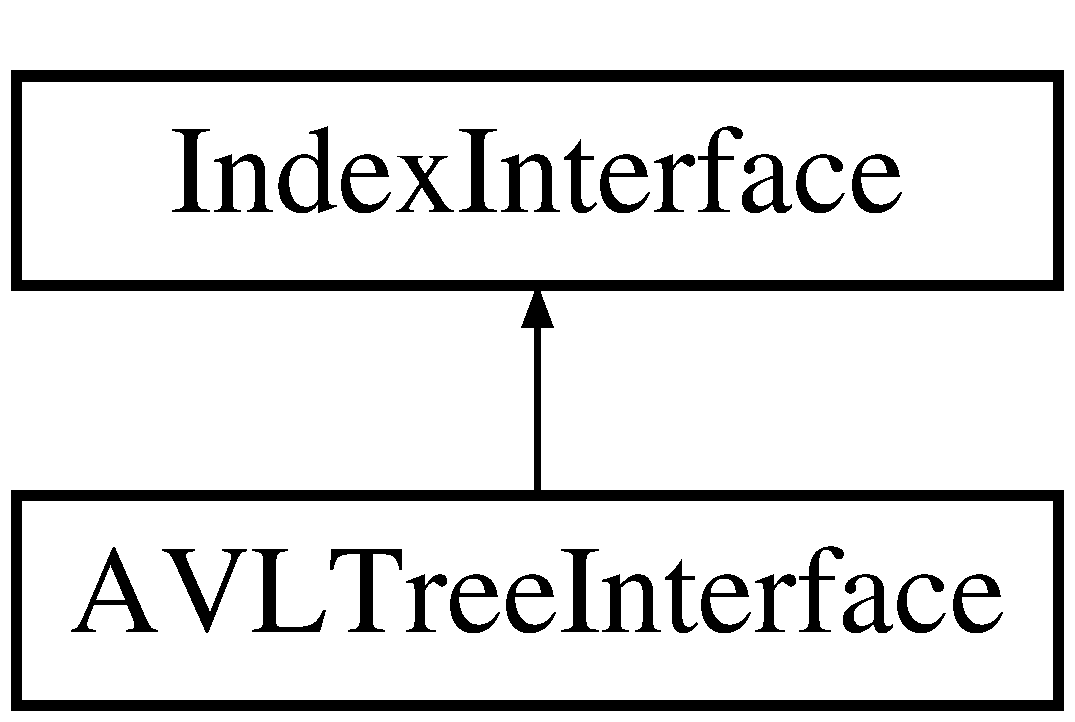
\includegraphics[height=2.000000cm]{class_a_v_l_tree_interface}
\end{center}
\end{figure}
\subsection*{Public Member Functions}
\begin{DoxyCompactItemize}
\item 
\hyperlink{class_a_v_l_tree_interface_abaec1061e3c1982382aeda27495af568}{A\+V\+L\+Tree\+Interface} ()
\begin{DoxyCompactList}\small\item\em constructor \end{DoxyCompactList}\item 
\hyperlink{class_a_v_l_tree_interface_a919ac950421b6702b2f82b9849b81108}{$\sim$\+A\+V\+L\+Tree\+Interface} ()
\begin{DoxyCompactList}\small\item\em destructor \end{DoxyCompactList}\item 
void \hyperlink{class_a_v_l_tree_interface_a2ff7466f1fd70ce6391330c04749fec7}{add\+\_\+term\+\_\+to\+\_\+ii} (int letter\+Index, \hyperlink{class_term}{Term} $\ast$term)
\begin{DoxyCompactList}\small\item\em adds term to the each individual avl\+Trees \end{DoxyCompactList}\item 
void \hyperlink{class_a_v_l_tree_interface_a748ffc895fb64aab3e2afac287f80630}{clear} ()
\begin{DoxyCompactList}\small\item\em clears avl\+Trees \end{DoxyCompactList}\item 
\hyperlink{class_term}{Term} $\ast$ \hyperlink{class_a_v_l_tree_interface_a35ee941b125e65cf0b5783a687503d83}{find\+\_\+term} (string term)
\begin{DoxyCompactList}\small\item\em searches each avl\+Trees for word and than returns term \end{DoxyCompactList}\item 
void \hyperlink{class_a_v_l_tree_interface_abd7f70746611a3982dc07a1b1880e7b5}{write\+\_\+persistence\+\_\+files} ()
\begin{DoxyCompactList}\small\item\em creates the persistance index \end{DoxyCompactList}\end{DoxyCompactItemize}
\subsection*{Additional Inherited Members}


\subsection{Detailed Description}
A\+V\+L Tree \hyperlink{class_interface}{Interface} implements 26 different \hyperlink{class_a_v_l_tree_index}{A\+V\+L\+Tree\+Index}\textquotesingle{}s. 

$<$ inherits virtual functions from \hyperlink{class_index_interface}{Index\+Interface} 

\subsection{Constructor \& Destructor Documentation}
\hypertarget{class_a_v_l_tree_interface_abaec1061e3c1982382aeda27495af568}{}\index{A\+V\+L\+Tree\+Interface@{A\+V\+L\+Tree\+Interface}!A\+V\+L\+Tree\+Interface@{A\+V\+L\+Tree\+Interface}}
\index{A\+V\+L\+Tree\+Interface@{A\+V\+L\+Tree\+Interface}!A\+V\+L\+Tree\+Interface@{A\+V\+L\+Tree\+Interface}}
\subsubsection[{A\+V\+L\+Tree\+Interface()}]{\setlength{\rightskip}{0pt plus 5cm}A\+V\+L\+Tree\+Interface\+::\+A\+V\+L\+Tree\+Interface (
\begin{DoxyParamCaption}
{}
\end{DoxyParamCaption}
)}\label{class_a_v_l_tree_interface_abaec1061e3c1982382aeda27495af568}


constructor 

\hyperlink{class_a_v_l_tree_interface}{A\+V\+L\+Tree\+Interface} creates 26 different A\+V\+L Trees. \hypertarget{class_a_v_l_tree_interface_a919ac950421b6702b2f82b9849b81108}{}\index{A\+V\+L\+Tree\+Interface@{A\+V\+L\+Tree\+Interface}!````~A\+V\+L\+Tree\+Interface@{$\sim$\+A\+V\+L\+Tree\+Interface}}
\index{````~A\+V\+L\+Tree\+Interface@{$\sim$\+A\+V\+L\+Tree\+Interface}!A\+V\+L\+Tree\+Interface@{A\+V\+L\+Tree\+Interface}}
\subsubsection[{$\sim$\+A\+V\+L\+Tree\+Interface()}]{\setlength{\rightskip}{0pt plus 5cm}A\+V\+L\+Tree\+Interface\+::$\sim$\+A\+V\+L\+Tree\+Interface (
\begin{DoxyParamCaption}
{}
\end{DoxyParamCaption}
)}\label{class_a_v_l_tree_interface_a919ac950421b6702b2f82b9849b81108}


destructor 

D\+E\+S\+T\+R\+U\+C\+T\+O\+R. 

\subsection{Member Function Documentation}
\hypertarget{class_a_v_l_tree_interface_a2ff7466f1fd70ce6391330c04749fec7}{}\index{A\+V\+L\+Tree\+Interface@{A\+V\+L\+Tree\+Interface}!add\+\_\+term\+\_\+to\+\_\+ii@{add\+\_\+term\+\_\+to\+\_\+ii}}
\index{add\+\_\+term\+\_\+to\+\_\+ii@{add\+\_\+term\+\_\+to\+\_\+ii}!A\+V\+L\+Tree\+Interface@{A\+V\+L\+Tree\+Interface}}
\subsubsection[{add\+\_\+term\+\_\+to\+\_\+ii(int letter\+Index, Term $\ast$term)}]{\setlength{\rightskip}{0pt plus 5cm}void A\+V\+L\+Tree\+Interface\+::add\+\_\+term\+\_\+to\+\_\+ii (
\begin{DoxyParamCaption}
\item[{int}]{letter\+Index, }
\item[{{\bf Term} $\ast$}]{term}
\end{DoxyParamCaption}
)\hspace{0.3cm}{\ttfamily [virtual]}}\label{class_a_v_l_tree_interface_a2ff7466f1fd70ce6391330c04749fec7}


adds term to the each individual avl\+Trees 



Reimplemented from \hyperlink{class_index_interface_aa83b7083d107869e3519c5862bc71d0a}{Index\+Interface}.

\hypertarget{class_a_v_l_tree_interface_a748ffc895fb64aab3e2afac287f80630}{}\index{A\+V\+L\+Tree\+Interface@{A\+V\+L\+Tree\+Interface}!clear@{clear}}
\index{clear@{clear}!A\+V\+L\+Tree\+Interface@{A\+V\+L\+Tree\+Interface}}
\subsubsection[{clear()}]{\setlength{\rightskip}{0pt plus 5cm}void A\+V\+L\+Tree\+Interface\+::clear (
\begin{DoxyParamCaption}
{}
\end{DoxyParamCaption}
)\hspace{0.3cm}{\ttfamily [virtual]}}\label{class_a_v_l_tree_interface_a748ffc895fb64aab3e2afac287f80630}


clears avl\+Trees 



Reimplemented from \hyperlink{class_index_interface_ad7b88501f360ccfad0c1ee08d793ca25}{Index\+Interface}.

\hypertarget{class_a_v_l_tree_interface_a35ee941b125e65cf0b5783a687503d83}{}\index{A\+V\+L\+Tree\+Interface@{A\+V\+L\+Tree\+Interface}!find\+\_\+term@{find\+\_\+term}}
\index{find\+\_\+term@{find\+\_\+term}!A\+V\+L\+Tree\+Interface@{A\+V\+L\+Tree\+Interface}}
\subsubsection[{find\+\_\+term(string term)}]{\setlength{\rightskip}{0pt plus 5cm}{\bf Term} $\ast$ A\+V\+L\+Tree\+Interface\+::find\+\_\+term (
\begin{DoxyParamCaption}
\item[{string}]{term}
\end{DoxyParamCaption}
)\hspace{0.3cm}{\ttfamily [virtual]}}\label{class_a_v_l_tree_interface_a35ee941b125e65cf0b5783a687503d83}


searches each avl\+Trees for word and than returns term 



Reimplemented from \hyperlink{class_index_interface_a851f0396f0b390cc9aa8cde270afffc9}{Index\+Interface}.

\hypertarget{class_a_v_l_tree_interface_abd7f70746611a3982dc07a1b1880e7b5}{}\index{A\+V\+L\+Tree\+Interface@{A\+V\+L\+Tree\+Interface}!write\+\_\+persistence\+\_\+files@{write\+\_\+persistence\+\_\+files}}
\index{write\+\_\+persistence\+\_\+files@{write\+\_\+persistence\+\_\+files}!A\+V\+L\+Tree\+Interface@{A\+V\+L\+Tree\+Interface}}
\subsubsection[{write\+\_\+persistence\+\_\+files()}]{\setlength{\rightskip}{0pt plus 5cm}void A\+V\+L\+Tree\+Interface\+::write\+\_\+persistence\+\_\+files (
\begin{DoxyParamCaption}
{}
\end{DoxyParamCaption}
)\hspace{0.3cm}{\ttfamily [virtual]}}\label{class_a_v_l_tree_interface_abd7f70746611a3982dc07a1b1880e7b5}


creates the persistance index 



Reimplemented from \hyperlink{class_index_interface_a0b4ec5fcc32c08959cffad3a3141dd4e}{Index\+Interface}.



The documentation for this class was generated from the following files\+:\begin{DoxyCompactItemize}
\item 
/\+Users/brandonmcfarland/\+Desktop/searchdocs/\+Search\+Engine/\+Final\+Project/\hyperlink{avltreeinterface_8h}{avltreeinterface.\+h}\item 
/\+Users/brandonmcfarland/\+Desktop/searchdocs/\+Search\+Engine/\+Final\+Project/\hyperlink{avltreeinterface_8cpp}{avltreeinterface.\+cpp}\end{DoxyCompactItemize}

\hypertarget{class_doc_parser}{}\section{Doc\+Parser Class Reference}
\label{class_doc_parser}\index{Doc\+Parser@{Doc\+Parser}}


Handles the text of files, primarily that of Wiki\+Books.\+xml. Uses Rapid\+X\+M\+L libraries. Initiates \hyperlink{class_page_info}{Page\+Info} objects for a file and stores them to the inverted index.  




{\ttfamily \#include $<$docparser.\+h$>$}

\subsection*{Public Member Functions}
\begin{DoxyCompactItemize}
\item 
\hyperlink{class_doc_parser_a637fc4d565eaf2927ee9b88bbe23e3cb}{$\sim$\+Doc\+Parser} ()
\item 
\hyperlink{class_doc_parser_a086f00e54fca8038c85c0e235948d75a}{Doc\+Parser} (\hyperlink{class_index_interface}{Index\+Interface} \&the\+Index)
\begin{DoxyCompactList}\small\item\em Default constructor never called; must take a reference to the inverted file intdex. \end{DoxyCompactList}\item 
string \hyperlink{class_doc_parser_a1b127af53e8af16f393b64f46c307d3a}{clean\+\_\+term} (string term)
\begin{DoxyCompactList}\small\item\em Stem the terms then makes all letters lowercase. \end{DoxyCompactList}\item 
void \hyperlink{class_doc_parser_ad92d1a6da7d413abd27ee18a6ed20a30}{clear} ()
\begin{DoxyCompactList}\small\item\em Deallocate data members. \end{DoxyCompactList}\item 
int \hyperlink{class_doc_parser_a7addc81ac337c2688bb9e9d8197db2fc}{index\+\_\+for\+\_\+letter} (char letter)
\begin{DoxyCompactList}\small\item\em Determine which \hyperlink{class_a_v_l_tree_index}{A\+V\+L\+Tree\+Index} or \hyperlink{class_hash_table_index}{Hash\+Table\+Index} should handle the appearance. Returns 0 if the term is a number, 1 for \textquotesingle{}a\textquotesingle{}, 2 for \textquotesingle{}b\textquotesingle{}, and so forth. \end{DoxyCompactList}\item 
void \hyperlink{class_doc_parser_a48cd3949baca573b9be0b4ba24b9c79d}{read\+\_\+page} (\hyperlink{classrapidxml_1_1xml__node}{xml\+\_\+node}$<$$>$ $\ast$curr\+Node, bool read\+Text)
\begin{DoxyCompactList}\small\item\em Makes a new \hyperlink{class_page_info}{Page\+Info} object from a page. Will or will not fetch term appearances from the text after using it as a \hyperlink{class_page_info}{Page\+Info} constructor parameter. \end{DoxyCompactList}\item 
void \hyperlink{class_doc_parser_af28153ebf0ee2fe97c2942c04c915adc}{read\+\_\+text} (\hyperlink{classrapidxml_1_1xml__node}{xml\+\_\+node}$<$$>$ $\ast$curr\+Node)
\begin{DoxyCompactList}\small\item\em Get all page appearances from the current page\textquotesingle{}s text. Pass this info to the inverted index. \end{DoxyCompactList}\item 
void \hyperlink{class_doc_parser_ad7b5809e4efd3e2bae781c1cb491ab29}{init\+\_\+file\+\_\+page\+\_\+infos} (\hyperlink{classrapidxml_1_1xml__node}{xml\+\_\+node}$<$$>$ $\ast$curr\+Node, bool read\+Text)
\begin{DoxyCompactList}\small\item\em Call read\+\_\+page for each page. \end{DoxyCompactList}\item 
void \hyperlink{class_doc_parser_a45860ee7fb0b956c4342cd4a815818de}{read\+\_\+file} (string file\+Path)
\begin{DoxyCompactList}\small\item\em Get to the right node (assuming it\textquotesingle{}s the same structure as Wiki\+Books.\+xml, then call init\+\_\+file\+\_\+page\+\_\+infos. \end{DoxyCompactList}\item 
bool \hyperlink{class_doc_parser_ad30c49de12ed45eaf2594c4718789c3e}{is\+\_\+stop\+\_\+word} (string term)
\begin{DoxyCompactList}\small\item\em Checks the stop\+Word\+Map; returns true if the passed string is in stop\+Words. \end{DoxyCompactList}\end{DoxyCompactItemize}


\subsection{Detailed Description}
Handles the text of files, primarily that of Wiki\+Books.\+xml. Uses Rapid\+X\+M\+L libraries. Initiates \hyperlink{class_page_info}{Page\+Info} objects for a file and stores them to the inverted index. 

\subsection{Constructor \& Destructor Documentation}
\hypertarget{class_doc_parser_a637fc4d565eaf2927ee9b88bbe23e3cb}{}\index{Doc\+Parser@{Doc\+Parser}!````~Doc\+Parser@{$\sim$\+Doc\+Parser}}
\index{````~Doc\+Parser@{$\sim$\+Doc\+Parser}!Doc\+Parser@{Doc\+Parser}}
\subsubsection[{$\sim$\+Doc\+Parser()}]{\setlength{\rightskip}{0pt plus 5cm}Doc\+Parser\+::$\sim$\+Doc\+Parser (
\begin{DoxyParamCaption}
{}
\end{DoxyParamCaption}
)}\label{class_doc_parser_a637fc4d565eaf2927ee9b88bbe23e3cb}
\hypertarget{class_doc_parser_a086f00e54fca8038c85c0e235948d75a}{}\index{Doc\+Parser@{Doc\+Parser}!Doc\+Parser@{Doc\+Parser}}
\index{Doc\+Parser@{Doc\+Parser}!Doc\+Parser@{Doc\+Parser}}
\subsubsection[{Doc\+Parser(\+Index\+Interface \&the\+Index)}]{\setlength{\rightskip}{0pt plus 5cm}Doc\+Parser\+::\+Doc\+Parser (
\begin{DoxyParamCaption}
\item[{{\bf Index\+Interface} \&}]{the\+Index}
\end{DoxyParamCaption}
)}\label{class_doc_parser_a086f00e54fca8038c85c0e235948d75a}


Default constructor never called; must take a reference to the inverted file intdex. 



\subsection{Member Function Documentation}
\hypertarget{class_doc_parser_a1b127af53e8af16f393b64f46c307d3a}{}\index{Doc\+Parser@{Doc\+Parser}!clean\+\_\+term@{clean\+\_\+term}}
\index{clean\+\_\+term@{clean\+\_\+term}!Doc\+Parser@{Doc\+Parser}}
\subsubsection[{clean\+\_\+term(string term)}]{\setlength{\rightskip}{0pt plus 5cm}string Doc\+Parser\+::clean\+\_\+term (
\begin{DoxyParamCaption}
\item[{string}]{term}
\end{DoxyParamCaption}
)}\label{class_doc_parser_a1b127af53e8af16f393b64f46c307d3a}


Stem the terms then makes all letters lowercase. 

\hypertarget{class_doc_parser_ad92d1a6da7d413abd27ee18a6ed20a30}{}\index{Doc\+Parser@{Doc\+Parser}!clear@{clear}}
\index{clear@{clear}!Doc\+Parser@{Doc\+Parser}}
\subsubsection[{clear()}]{\setlength{\rightskip}{0pt plus 5cm}void Doc\+Parser\+::clear (
\begin{DoxyParamCaption}
{}
\end{DoxyParamCaption}
)}\label{class_doc_parser_ad92d1a6da7d413abd27ee18a6ed20a30}


Deallocate data members. 

\hypertarget{class_doc_parser_a7addc81ac337c2688bb9e9d8197db2fc}{}\index{Doc\+Parser@{Doc\+Parser}!index\+\_\+for\+\_\+letter@{index\+\_\+for\+\_\+letter}}
\index{index\+\_\+for\+\_\+letter@{index\+\_\+for\+\_\+letter}!Doc\+Parser@{Doc\+Parser}}
\subsubsection[{index\+\_\+for\+\_\+letter(char letter)}]{\setlength{\rightskip}{0pt plus 5cm}int Doc\+Parser\+::index\+\_\+for\+\_\+letter (
\begin{DoxyParamCaption}
\item[{char}]{letter}
\end{DoxyParamCaption}
)}\label{class_doc_parser_a7addc81ac337c2688bb9e9d8197db2fc}


Determine which \hyperlink{class_a_v_l_tree_index}{A\+V\+L\+Tree\+Index} or \hyperlink{class_hash_table_index}{Hash\+Table\+Index} should handle the appearance. Returns 0 if the term is a number, 1 for \textquotesingle{}a\textquotesingle{}, 2 for \textquotesingle{}b\textquotesingle{}, and so forth. 

\hypertarget{class_doc_parser_ad7b5809e4efd3e2bae781c1cb491ab29}{}\index{Doc\+Parser@{Doc\+Parser}!init\+\_\+file\+\_\+page\+\_\+infos@{init\+\_\+file\+\_\+page\+\_\+infos}}
\index{init\+\_\+file\+\_\+page\+\_\+infos@{init\+\_\+file\+\_\+page\+\_\+infos}!Doc\+Parser@{Doc\+Parser}}
\subsubsection[{init\+\_\+file\+\_\+page\+\_\+infos(xml\+\_\+node$<$$>$ $\ast$curr\+Node, bool read\+Text)}]{\setlength{\rightskip}{0pt plus 5cm}void Doc\+Parser\+::init\+\_\+file\+\_\+page\+\_\+infos (
\begin{DoxyParamCaption}
\item[{{\bf xml\+\_\+node}$<$$>$ $\ast$}]{curr\+Node, }
\item[{bool}]{read\+Text}
\end{DoxyParamCaption}
)}\label{class_doc_parser_ad7b5809e4efd3e2bae781c1cb491ab29}


Call read\+\_\+page for each page. 

\hypertarget{class_doc_parser_ad30c49de12ed45eaf2594c4718789c3e}{}\index{Doc\+Parser@{Doc\+Parser}!is\+\_\+stop\+\_\+word@{is\+\_\+stop\+\_\+word}}
\index{is\+\_\+stop\+\_\+word@{is\+\_\+stop\+\_\+word}!Doc\+Parser@{Doc\+Parser}}
\subsubsection[{is\+\_\+stop\+\_\+word(string term)}]{\setlength{\rightskip}{0pt plus 5cm}bool Doc\+Parser\+::is\+\_\+stop\+\_\+word (
\begin{DoxyParamCaption}
\item[{string}]{term}
\end{DoxyParamCaption}
)}\label{class_doc_parser_ad30c49de12ed45eaf2594c4718789c3e}


Checks the stop\+Word\+Map; returns true if the passed string is in stop\+Words. 

\hypertarget{class_doc_parser_a45860ee7fb0b956c4342cd4a815818de}{}\index{Doc\+Parser@{Doc\+Parser}!read\+\_\+file@{read\+\_\+file}}
\index{read\+\_\+file@{read\+\_\+file}!Doc\+Parser@{Doc\+Parser}}
\subsubsection[{read\+\_\+file(string file\+Path)}]{\setlength{\rightskip}{0pt plus 5cm}void Doc\+Parser\+::read\+\_\+file (
\begin{DoxyParamCaption}
\item[{string}]{file\+Path}
\end{DoxyParamCaption}
)}\label{class_doc_parser_a45860ee7fb0b956c4342cd4a815818de}


Get to the right node (assuming it\textquotesingle{}s the same structure as Wiki\+Books.\+xml, then call init\+\_\+file\+\_\+page\+\_\+infos. 

\hypertarget{class_doc_parser_a48cd3949baca573b9be0b4ba24b9c79d}{}\index{Doc\+Parser@{Doc\+Parser}!read\+\_\+page@{read\+\_\+page}}
\index{read\+\_\+page@{read\+\_\+page}!Doc\+Parser@{Doc\+Parser}}
\subsubsection[{read\+\_\+page(xml\+\_\+node$<$$>$ $\ast$curr\+Node, bool read\+Text)}]{\setlength{\rightskip}{0pt plus 5cm}void Doc\+Parser\+::read\+\_\+page (
\begin{DoxyParamCaption}
\item[{{\bf xml\+\_\+node}$<$$>$ $\ast$}]{curr\+Node, }
\item[{bool}]{read\+Text}
\end{DoxyParamCaption}
)}\label{class_doc_parser_a48cd3949baca573b9be0b4ba24b9c79d}


Makes a new \hyperlink{class_page_info}{Page\+Info} object from a page. Will or will not fetch term appearances from the text after using it as a \hyperlink{class_page_info}{Page\+Info} constructor parameter. 

\hypertarget{class_doc_parser_af28153ebf0ee2fe97c2942c04c915adc}{}\index{Doc\+Parser@{Doc\+Parser}!read\+\_\+text@{read\+\_\+text}}
\index{read\+\_\+text@{read\+\_\+text}!Doc\+Parser@{Doc\+Parser}}
\subsubsection[{read\+\_\+text(xml\+\_\+node$<$$>$ $\ast$curr\+Node)}]{\setlength{\rightskip}{0pt plus 5cm}void Doc\+Parser\+::read\+\_\+text (
\begin{DoxyParamCaption}
\item[{{\bf xml\+\_\+node}$<$$>$ $\ast$}]{curr\+Node}
\end{DoxyParamCaption}
)}\label{class_doc_parser_af28153ebf0ee2fe97c2942c04c915adc}


Get all page appearances from the current page\textquotesingle{}s text. Pass this info to the inverted index. 



The documentation for this class was generated from the following files\+:\begin{DoxyCompactItemize}
\item 
/\+Users/brandonmcfarland/\+Desktop/searchdocs/\+Search\+Engine/\+Final\+Project/\hyperlink{docparser_8h}{docparser.\+h}\item 
/\+Users/brandonmcfarland/\+Desktop/searchdocs/\+Search\+Engine/\+Final\+Project/\hyperlink{docparser_8cpp}{docparser.\+cpp}\end{DoxyCompactItemize}

\hypertarget{classrapidxml_1_1file}{}\section{rapidxml\+:\+:file$<$ Ch $>$ Class Template Reference}
\label{classrapidxml_1_1file}\index{rapidxml\+::file$<$ Ch $>$@{rapidxml\+::file$<$ Ch $>$}}


Represents data loaded from a file.  




{\ttfamily \#include $<$rapidxml\+\_\+utils.\+hpp$>$}

\subsection*{Public Member Functions}
\begin{DoxyCompactItemize}
\item 
\hyperlink{classrapidxml_1_1file_ae881a3cab1fe7152d45c92a8d7606cb3}{file} (const char $\ast$filename)
\item 
\hyperlink{classrapidxml_1_1file_a90707ccd991cc392dcf4bef37eed9d1f}{file} (std\+::basic\+\_\+istream$<$ Ch $>$ \&stream)
\item 
Ch $\ast$ \hyperlink{classrapidxml_1_1file_af1c71d65862c7af14e4708e32a80c1de}{data} ()
\item 
const Ch $\ast$ \hyperlink{classrapidxml_1_1file_aceb8f5ebd577c946a74b1ea3e2e0c576}{data} () const 
\item 
std\+::size\+\_\+t \hyperlink{classrapidxml_1_1file_a20191d167c6e00a88a44ca9a3a54e1c5}{size} () const 
\end{DoxyCompactItemize}


\subsection{Detailed Description}
\subsubsection*{template$<$class Ch = char$>$class rapidxml\+::file$<$ Ch $>$}

Represents data loaded from a file. 

\subsection{Constructor \& Destructor Documentation}
\hypertarget{classrapidxml_1_1file_ae881a3cab1fe7152d45c92a8d7606cb3}{}\index{rapidxml\+::file@{rapidxml\+::file}!file@{file}}
\index{file@{file}!rapidxml\+::file@{rapidxml\+::file}}
\subsubsection[{file(const char $\ast$filename)}]{\setlength{\rightskip}{0pt plus 5cm}template$<$class Ch  = char$>$ {\bf rapidxml\+::file}$<$ Ch $>$\+::{\bf file} (
\begin{DoxyParamCaption}
\item[{const char $\ast$}]{filename}
\end{DoxyParamCaption}
)\hspace{0.3cm}{\ttfamily [inline]}}\label{classrapidxml_1_1file_ae881a3cab1fe7152d45c92a8d7606cb3}
Loads file into the memory. Data will be automatically destroyed by the destructor. 
\begin{DoxyParams}{Parameters}
{\em filename} & Filename to load. \\
\hline
\end{DoxyParams}
\hypertarget{classrapidxml_1_1file_a90707ccd991cc392dcf4bef37eed9d1f}{}\index{rapidxml\+::file@{rapidxml\+::file}!file@{file}}
\index{file@{file}!rapidxml\+::file@{rapidxml\+::file}}
\subsubsection[{file(std\+::basic\+\_\+istream$<$ Ch $>$ \&stream)}]{\setlength{\rightskip}{0pt plus 5cm}template$<$class Ch  = char$>$ {\bf rapidxml\+::file}$<$ Ch $>$\+::{\bf file} (
\begin{DoxyParamCaption}
\item[{std\+::basic\+\_\+istream$<$ Ch $>$ \&}]{stream}
\end{DoxyParamCaption}
)\hspace{0.3cm}{\ttfamily [inline]}}\label{classrapidxml_1_1file_a90707ccd991cc392dcf4bef37eed9d1f}
Loads file into the memory. Data will be automatically destroyed by the destructor 
\begin{DoxyParams}{Parameters}
{\em stream} & Stream to load from \\
\hline
\end{DoxyParams}


\subsection{Member Function Documentation}
\hypertarget{classrapidxml_1_1file_af1c71d65862c7af14e4708e32a80c1de}{}\index{rapidxml\+::file@{rapidxml\+::file}!data@{data}}
\index{data@{data}!rapidxml\+::file@{rapidxml\+::file}}
\subsubsection[{data()}]{\setlength{\rightskip}{0pt plus 5cm}template$<$class Ch  = char$>$ Ch$\ast$ {\bf rapidxml\+::file}$<$ Ch $>$\+::data (
\begin{DoxyParamCaption}
{}
\end{DoxyParamCaption}
)\hspace{0.3cm}{\ttfamily [inline]}}\label{classrapidxml_1_1file_af1c71d65862c7af14e4708e32a80c1de}
Gets file data. \begin{DoxyReturn}{Returns}
Pointer to data of file. 
\end{DoxyReturn}
\hypertarget{classrapidxml_1_1file_aceb8f5ebd577c946a74b1ea3e2e0c576}{}\index{rapidxml\+::file@{rapidxml\+::file}!data@{data}}
\index{data@{data}!rapidxml\+::file@{rapidxml\+::file}}
\subsubsection[{data() const }]{\setlength{\rightskip}{0pt plus 5cm}template$<$class Ch  = char$>$ const Ch$\ast$ {\bf rapidxml\+::file}$<$ Ch $>$\+::data (
\begin{DoxyParamCaption}
{}
\end{DoxyParamCaption}
) const\hspace{0.3cm}{\ttfamily [inline]}}\label{classrapidxml_1_1file_aceb8f5ebd577c946a74b1ea3e2e0c576}
Gets file data. \begin{DoxyReturn}{Returns}
Pointer to data of file. 
\end{DoxyReturn}
\hypertarget{classrapidxml_1_1file_a20191d167c6e00a88a44ca9a3a54e1c5}{}\index{rapidxml\+::file@{rapidxml\+::file}!size@{size}}
\index{size@{size}!rapidxml\+::file@{rapidxml\+::file}}
\subsubsection[{size() const }]{\setlength{\rightskip}{0pt plus 5cm}template$<$class Ch  = char$>$ std\+::size\+\_\+t {\bf rapidxml\+::file}$<$ Ch $>$\+::size (
\begin{DoxyParamCaption}
{}
\end{DoxyParamCaption}
) const\hspace{0.3cm}{\ttfamily [inline]}}\label{classrapidxml_1_1file_a20191d167c6e00a88a44ca9a3a54e1c5}
Gets file data size. \begin{DoxyReturn}{Returns}
Size of file data, in characters. 
\end{DoxyReturn}


The documentation for this class was generated from the following file\+:\begin{DoxyCompactItemize}
\item 
/\+Users/brandonmcfarland/\+Desktop/searchdocs/\+Search\+Engine/\+Final\+Project/\hyperlink{rapidxml__utils_8hpp}{rapidxml\+\_\+utils.\+hpp}\end{DoxyCompactItemize}

\hypertarget{class_hash_table_index}{}\section{Hash\+Table\+Index Class Reference}
\label{class_hash_table_index}\index{Hash\+Table\+Index@{Hash\+Table\+Index}}


Holds 1024 Term\+Buckets. Hashes strings to map to Term$\ast$ values. Handles collisions with chaining.  




{\ttfamily \#include $<$hashtableindex.\+h$>$}

\subsection*{Public Member Functions}
\begin{DoxyCompactItemize}
\item 
\hyperlink{class_hash_table_index_a13c1c8deae84226c8bef382adf103b53}{Hash\+Table\+Index} ()
\item 
\hyperlink{class_hash_table_index_af4d2eeae8263c353f91140cb2583fb58}{$\sim$\+Hash\+Table\+Index} ()
\item 
void \hyperlink{class_hash_table_index_a383ac825c3dde6dd2791bb121da7138d}{add\+\_\+term\+\_\+to\+\_\+ht\+\_\+index} (\hyperlink{class_term}{Term} $\ast$term)
\begin{DoxyCompactList}\small\item\em Call add\+\_\+term\+\_\+to\+\_\+bucket at the hashed bucket. \end{DoxyCompactList}\item 
\hyperlink{class_term}{Term} $\ast$ \hyperlink{class_hash_table_index_a5934917eb943ab770d86ab7ff9142aab}{find} (string term)
\begin{DoxyCompactList}\small\item\em Return Term$\ast$ (matching the passed string) from the inverted index. Return N\+U\+L\+L if none is found. \end{DoxyCompactList}\item 
int \hyperlink{class_hash_table_index_a93a1393996af092def6a7f2b9156f2c6}{hash\+\_\+key} (string key)
\begin{DoxyCompactList}\small\item\em Custom hash function. Specifics in \hyperlink{hashtableindex_8cpp}{hashtableindex.\+cpp}. \end{DoxyCompactList}\item 
void \hyperlink{class_hash_table_index_a8ed7978b35943e4b89526bb5d7017f05}{write\+\_\+hti} (ofstream \&persistence)
\begin{DoxyCompactList}\small\item\em Call write\+\_\+term\+\_\+bucket for the hashed bucket. \end{DoxyCompactList}\item 
void \hyperlink{class_hash_table_index_a253a51a2195d47b3350fdc27fd3d4077}{clear\+\_\+table} ()
\begin{DoxyCompactList}\small\item\em Deallocate data members. \end{DoxyCompactList}\end{DoxyCompactItemize}


\subsection{Detailed Description}
Holds 1024 Term\+Buckets. Hashes strings to map to Term$\ast$ values. Handles collisions with chaining. 

\subsection{Constructor \& Destructor Documentation}
\hypertarget{class_hash_table_index_a13c1c8deae84226c8bef382adf103b53}{}\index{Hash\+Table\+Index@{Hash\+Table\+Index}!Hash\+Table\+Index@{Hash\+Table\+Index}}
\index{Hash\+Table\+Index@{Hash\+Table\+Index}!Hash\+Table\+Index@{Hash\+Table\+Index}}
\subsubsection[{Hash\+Table\+Index()}]{\setlength{\rightskip}{0pt plus 5cm}Hash\+Table\+Index\+::\+Hash\+Table\+Index (
\begin{DoxyParamCaption}
{}
\end{DoxyParamCaption}
)}\label{class_hash_table_index_a13c1c8deae84226c8bef382adf103b53}
\hypertarget{class_hash_table_index_af4d2eeae8263c353f91140cb2583fb58}{}\index{Hash\+Table\+Index@{Hash\+Table\+Index}!````~Hash\+Table\+Index@{$\sim$\+Hash\+Table\+Index}}
\index{````~Hash\+Table\+Index@{$\sim$\+Hash\+Table\+Index}!Hash\+Table\+Index@{Hash\+Table\+Index}}
\subsubsection[{$\sim$\+Hash\+Table\+Index()}]{\setlength{\rightskip}{0pt plus 5cm}Hash\+Table\+Index\+::$\sim$\+Hash\+Table\+Index (
\begin{DoxyParamCaption}
{}
\end{DoxyParamCaption}
)}\label{class_hash_table_index_af4d2eeae8263c353f91140cb2583fb58}


\subsection{Member Function Documentation}
\hypertarget{class_hash_table_index_a383ac825c3dde6dd2791bb121da7138d}{}\index{Hash\+Table\+Index@{Hash\+Table\+Index}!add\+\_\+term\+\_\+to\+\_\+ht\+\_\+index@{add\+\_\+term\+\_\+to\+\_\+ht\+\_\+index}}
\index{add\+\_\+term\+\_\+to\+\_\+ht\+\_\+index@{add\+\_\+term\+\_\+to\+\_\+ht\+\_\+index}!Hash\+Table\+Index@{Hash\+Table\+Index}}
\subsubsection[{add\+\_\+term\+\_\+to\+\_\+ht\+\_\+index(\+Term $\ast$term)}]{\setlength{\rightskip}{0pt plus 5cm}void Hash\+Table\+Index\+::add\+\_\+term\+\_\+to\+\_\+ht\+\_\+index (
\begin{DoxyParamCaption}
\item[{{\bf Term} $\ast$}]{term}
\end{DoxyParamCaption}
)}\label{class_hash_table_index_a383ac825c3dde6dd2791bb121da7138d}


Call add\+\_\+term\+\_\+to\+\_\+bucket at the hashed bucket. 

\hypertarget{class_hash_table_index_a253a51a2195d47b3350fdc27fd3d4077}{}\index{Hash\+Table\+Index@{Hash\+Table\+Index}!clear\+\_\+table@{clear\+\_\+table}}
\index{clear\+\_\+table@{clear\+\_\+table}!Hash\+Table\+Index@{Hash\+Table\+Index}}
\subsubsection[{clear\+\_\+table()}]{\setlength{\rightskip}{0pt plus 5cm}void Hash\+Table\+Index\+::clear\+\_\+table (
\begin{DoxyParamCaption}
{}
\end{DoxyParamCaption}
)}\label{class_hash_table_index_a253a51a2195d47b3350fdc27fd3d4077}


Deallocate data members. 

\hypertarget{class_hash_table_index_a5934917eb943ab770d86ab7ff9142aab}{}\index{Hash\+Table\+Index@{Hash\+Table\+Index}!find@{find}}
\index{find@{find}!Hash\+Table\+Index@{Hash\+Table\+Index}}
\subsubsection[{find(string term)}]{\setlength{\rightskip}{0pt plus 5cm}{\bf Term} $\ast$ Hash\+Table\+Index\+::find (
\begin{DoxyParamCaption}
\item[{string}]{term}
\end{DoxyParamCaption}
)}\label{class_hash_table_index_a5934917eb943ab770d86ab7ff9142aab}


Return Term$\ast$ (matching the passed string) from the inverted index. Return N\+U\+L\+L if none is found. 

\hypertarget{class_hash_table_index_a93a1393996af092def6a7f2b9156f2c6}{}\index{Hash\+Table\+Index@{Hash\+Table\+Index}!hash\+\_\+key@{hash\+\_\+key}}
\index{hash\+\_\+key@{hash\+\_\+key}!Hash\+Table\+Index@{Hash\+Table\+Index}}
\subsubsection[{hash\+\_\+key(string key)}]{\setlength{\rightskip}{0pt plus 5cm}int Hash\+Table\+Index\+::hash\+\_\+key (
\begin{DoxyParamCaption}
\item[{string}]{key}
\end{DoxyParamCaption}
)}\label{class_hash_table_index_a93a1393996af092def6a7f2b9156f2c6}


Custom hash function. Specifics in \hyperlink{hashtableindex_8cpp}{hashtableindex.\+cpp}. 

\hypertarget{class_hash_table_index_a8ed7978b35943e4b89526bb5d7017f05}{}\index{Hash\+Table\+Index@{Hash\+Table\+Index}!write\+\_\+hti@{write\+\_\+hti}}
\index{write\+\_\+hti@{write\+\_\+hti}!Hash\+Table\+Index@{Hash\+Table\+Index}}
\subsubsection[{write\+\_\+hti(ofstream \&persistence)}]{\setlength{\rightskip}{0pt plus 5cm}void Hash\+Table\+Index\+::write\+\_\+hti (
\begin{DoxyParamCaption}
\item[{ofstream \&}]{persistence}
\end{DoxyParamCaption}
)}\label{class_hash_table_index_a8ed7978b35943e4b89526bb5d7017f05}


Call write\+\_\+term\+\_\+bucket for the hashed bucket. 



The documentation for this class was generated from the following files\+:\begin{DoxyCompactItemize}
\item 
/\+Users/brandonmcfarland/\+Desktop/searchdocs/\+Search\+Engine/\+Final\+Project/\hyperlink{hashtableindex_8h}{hashtableindex.\+h}\item 
/\+Users/brandonmcfarland/\+Desktop/searchdocs/\+Search\+Engine/\+Final\+Project/\hyperlink{hashtableindex_8cpp}{hashtableindex.\+cpp}\end{DoxyCompactItemize}

\hypertarget{class_hash_table_interface}{}\section{Hash\+Table\+Interface Class Reference}
\label{class_hash_table_interface}\index{Hash\+Table\+Interface@{Hash\+Table\+Interface}}


Holds 26 Hash\+Table\+Indexes, one for each letter of the alphabet. Inherits from \hyperlink{class_index_interface}{Index\+Interface}.  




{\ttfamily \#include $<$hashtableinterface.\+h$>$}

Inheritance diagram for Hash\+Table\+Interface\+:\begin{figure}[H]
\begin{center}
\leavevmode
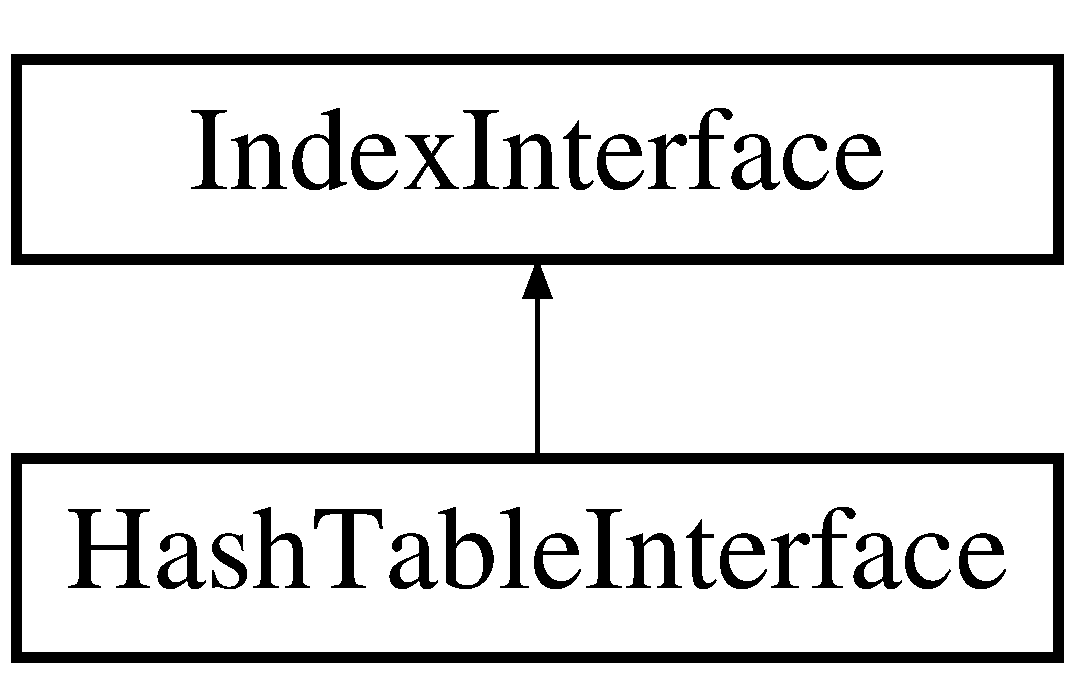
\includegraphics[height=2.000000cm]{class_hash_table_interface}
\end{center}
\end{figure}
\subsection*{Public Member Functions}
\begin{DoxyCompactItemize}
\item 
\hyperlink{class_hash_table_interface_afcc090bbeda66c331a7a28623aad5d0c}{Hash\+Table\+Interface} ()
\item 
\hyperlink{class_hash_table_interface_ab0a34d3f1ee275590002fc4c5d4327fe}{$\sim$\+Hash\+Table\+Interface} ()
\end{DoxyCompactItemize}
\subsection*{Additional Inherited Members}


\subsection{Detailed Description}
Holds 26 Hash\+Table\+Indexes, one for each letter of the alphabet. Inherits from \hyperlink{class_index_interface}{Index\+Interface}. 

\subsection{Constructor \& Destructor Documentation}
\hypertarget{class_hash_table_interface_afcc090bbeda66c331a7a28623aad5d0c}{}\index{Hash\+Table\+Interface@{Hash\+Table\+Interface}!Hash\+Table\+Interface@{Hash\+Table\+Interface}}
\index{Hash\+Table\+Interface@{Hash\+Table\+Interface}!Hash\+Table\+Interface@{Hash\+Table\+Interface}}
\subsubsection[{Hash\+Table\+Interface()}]{\setlength{\rightskip}{0pt plus 5cm}Hash\+Table\+Interface\+::\+Hash\+Table\+Interface (
\begin{DoxyParamCaption}
{}
\end{DoxyParamCaption}
)}\label{class_hash_table_interface_afcc090bbeda66c331a7a28623aad5d0c}
\hypertarget{class_hash_table_interface_ab0a34d3f1ee275590002fc4c5d4327fe}{}\index{Hash\+Table\+Interface@{Hash\+Table\+Interface}!````~Hash\+Table\+Interface@{$\sim$\+Hash\+Table\+Interface}}
\index{````~Hash\+Table\+Interface@{$\sim$\+Hash\+Table\+Interface}!Hash\+Table\+Interface@{Hash\+Table\+Interface}}
\subsubsection[{$\sim$\+Hash\+Table\+Interface()}]{\setlength{\rightskip}{0pt plus 5cm}Hash\+Table\+Interface\+::$\sim$\+Hash\+Table\+Interface (
\begin{DoxyParamCaption}
{}
\end{DoxyParamCaption}
)}\label{class_hash_table_interface_ab0a34d3f1ee275590002fc4c5d4327fe}


The documentation for this class was generated from the following files\+:\begin{DoxyCompactItemize}
\item 
/\+Users/brandonmcfarland/\+Desktop/searchdocs/\+Search\+Engine/\+Final\+Project/\hyperlink{hashtableinterface_8h}{hashtableinterface.\+h}\item 
/\+Users/brandonmcfarland/\+Desktop/searchdocs/\+Search\+Engine/\+Final\+Project/\hyperlink{hashtableinterface_8cpp}{hashtableinterface.\+cpp}\end{DoxyCompactItemize}

\hypertarget{class_index_handler}{}\section{Index\+Handler Class Reference}
\label{class_index_handler}\index{Index\+Handler@{Index\+Handler}}


Connects \hyperlink{class_interface}{Interface} and \hyperlink{class_index_interface}{Index\+Interface}. Will construct either a \hyperlink{class_hash_table_index}{Hash\+Table\+Index} or \hyperlink{class_a_v_l_tree_index}{A\+V\+L\+Tree\+Index} and mediate between user commands and stored info.  




{\ttfamily \#include $<$indexhandler.\+h$>$}

\subsection*{Public Member Functions}
\begin{DoxyCompactItemize}
\item 
\hyperlink{class_index_handler_a27748387661142a2eb545be6f0499996}{Index\+Handler} ()
\item 
\hyperlink{class_index_handler_ad787ca8cf83345ecfe332d2c3b8f8009}{$\sim$\+Index\+Handler} ()
\item 
\hyperlink{class_index_handler_ae50be3bec7e5ad3ede66110535043e15}{Index\+Handler} (bool as\+Hash\+Table)
\begin{DoxyCompactList}\small\item\em Lets the user choose between data structures. \end{DoxyCompactList}\item 
void \hyperlink{class_index_handler_a3fe9b3c1b3df7eea7e4ae590df4a4339}{read\+\_\+file} (string file\+Path)
\begin{DoxyCompactList}\small\item\em Reads info for a given file\+Path. \end{DoxyCompactList}\item 
void \hyperlink{class_index_handler_acee974285412a635c3c31fe86b9e0fb8}{run\+\_\+queries} (string query)
\begin{DoxyCompactList}\small\item\em Call run\+\_\+queries in \hyperlink{class_index_interface}{Index\+Interface}. \end{DoxyCompactList}\item 
void \hyperlink{class_index_handler_a417830272cfc725f6966c7a0a0ceae1d}{clear\+\_\+index} ()
\begin{DoxyCompactList}\small\item\em Deallocate data members. \end{DoxyCompactList}\end{DoxyCompactItemize}


\subsection{Detailed Description}
Connects \hyperlink{class_interface}{Interface} and \hyperlink{class_index_interface}{Index\+Interface}. Will construct either a \hyperlink{class_hash_table_index}{Hash\+Table\+Index} or \hyperlink{class_a_v_l_tree_index}{A\+V\+L\+Tree\+Index} and mediate between user commands and stored info. 

\subsection{Constructor \& Destructor Documentation}
\hypertarget{class_index_handler_a27748387661142a2eb545be6f0499996}{}\index{Index\+Handler@{Index\+Handler}!Index\+Handler@{Index\+Handler}}
\index{Index\+Handler@{Index\+Handler}!Index\+Handler@{Index\+Handler}}
\subsubsection[{Index\+Handler()}]{\setlength{\rightskip}{0pt plus 5cm}Index\+Handler\+::\+Index\+Handler (
\begin{DoxyParamCaption}
{}
\end{DoxyParamCaption}
)}\label{class_index_handler_a27748387661142a2eb545be6f0499996}
\hypertarget{class_index_handler_ad787ca8cf83345ecfe332d2c3b8f8009}{}\index{Index\+Handler@{Index\+Handler}!````~Index\+Handler@{$\sim$\+Index\+Handler}}
\index{````~Index\+Handler@{$\sim$\+Index\+Handler}!Index\+Handler@{Index\+Handler}}
\subsubsection[{$\sim$\+Index\+Handler()}]{\setlength{\rightskip}{0pt plus 5cm}Index\+Handler\+::$\sim$\+Index\+Handler (
\begin{DoxyParamCaption}
{}
\end{DoxyParamCaption}
)}\label{class_index_handler_ad787ca8cf83345ecfe332d2c3b8f8009}
\hypertarget{class_index_handler_ae50be3bec7e5ad3ede66110535043e15}{}\index{Index\+Handler@{Index\+Handler}!Index\+Handler@{Index\+Handler}}
\index{Index\+Handler@{Index\+Handler}!Index\+Handler@{Index\+Handler}}
\subsubsection[{Index\+Handler(bool as\+Hash\+Table)}]{\setlength{\rightskip}{0pt plus 5cm}Index\+Handler\+::\+Index\+Handler (
\begin{DoxyParamCaption}
\item[{bool}]{as\+Hash\+Table}
\end{DoxyParamCaption}
)}\label{class_index_handler_ae50be3bec7e5ad3ede66110535043e15}


Lets the user choose between data structures. 



\subsection{Member Function Documentation}
\hypertarget{class_index_handler_a417830272cfc725f6966c7a0a0ceae1d}{}\index{Index\+Handler@{Index\+Handler}!clear\+\_\+index@{clear\+\_\+index}}
\index{clear\+\_\+index@{clear\+\_\+index}!Index\+Handler@{Index\+Handler}}
\subsubsection[{clear\+\_\+index()}]{\setlength{\rightskip}{0pt plus 5cm}void Index\+Handler\+::clear\+\_\+index (
\begin{DoxyParamCaption}
{}
\end{DoxyParamCaption}
)}\label{class_index_handler_a417830272cfc725f6966c7a0a0ceae1d}


Deallocate data members. 

\hypertarget{class_index_handler_a3fe9b3c1b3df7eea7e4ae590df4a4339}{}\index{Index\+Handler@{Index\+Handler}!read\+\_\+file@{read\+\_\+file}}
\index{read\+\_\+file@{read\+\_\+file}!Index\+Handler@{Index\+Handler}}
\subsubsection[{read\+\_\+file(string file\+Path)}]{\setlength{\rightskip}{0pt plus 5cm}void Index\+Handler\+::read\+\_\+file (
\begin{DoxyParamCaption}
\item[{string}]{file\+Path}
\end{DoxyParamCaption}
)}\label{class_index_handler_a3fe9b3c1b3df7eea7e4ae590df4a4339}


Reads info for a given file\+Path. 

\hypertarget{class_index_handler_acee974285412a635c3c31fe86b9e0fb8}{}\index{Index\+Handler@{Index\+Handler}!run\+\_\+queries@{run\+\_\+queries}}
\index{run\+\_\+queries@{run\+\_\+queries}!Index\+Handler@{Index\+Handler}}
\subsubsection[{run\+\_\+queries(string query)}]{\setlength{\rightskip}{0pt plus 5cm}void Index\+Handler\+::run\+\_\+queries (
\begin{DoxyParamCaption}
\item[{string}]{query}
\end{DoxyParamCaption}
)}\label{class_index_handler_acee974285412a635c3c31fe86b9e0fb8}


Call run\+\_\+queries in \hyperlink{class_index_interface}{Index\+Interface}. 



The documentation for this class was generated from the following files\+:\begin{DoxyCompactItemize}
\item 
/\+Users/brandonmcfarland/\+Desktop/searchdocs/\+Search\+Engine/\+Final\+Project/\hyperlink{indexhandler_8h}{indexhandler.\+h}\item 
/\+Users/brandonmcfarland/\+Desktop/searchdocs/\+Search\+Engine/\+Final\+Project/\hyperlink{indexhandler_8cpp}{indexhandler.\+cpp}\end{DoxyCompactItemize}

\hypertarget{class_index_interface}{}\section{Index\+Interface Class Reference}
\label{class_index_interface}\index{Index\+Interface@{Index\+Interface}}


The inverted file index. Two derived classes, \hyperlink{class_hash_table_interface}{Hash\+Table\+Interface} and \hyperlink{class_a_v_l_tree_interface}{A\+V\+L\+Tree\+Interface}, store the inverted file index as a hash table and A\+V\+L tree, respectively. Also holds total\+Words\+In\+Corpus for T\+D/\+I\+D\+F calculation. All virtual functions in this header implemented in \hyperlink{hashtableinterface_8cpp}{Hash\+Table\+Interface.\+cpp}. \hyperlink{class_a_v_l_tree_interface}{A\+V\+L\+Tree\+Interface} redefines said virtual functions.  




{\ttfamily \#include $<$indexinterface.\+h$>$}

Inheritance diagram for Index\+Interface\+:\begin{figure}[H]
\begin{center}
\leavevmode
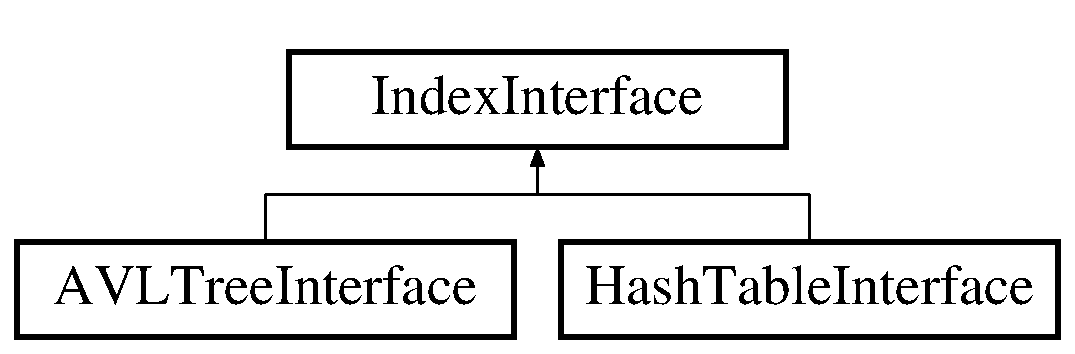
\includegraphics[height=2.000000cm]{class_index_interface}
\end{center}
\end{figure}
\subsection*{Public Member Functions}
\begin{DoxyCompactItemize}
\item 
\hyperlink{class_index_interface_a7b1e7eae7faa652d2f63efeecf0ca2de}{Index\+Interface} ()
\item 
\hyperlink{class_index_interface_a3927fabe77a7da5845dc0495b2c1c2b2}{$\sim$\+Index\+Interface} ()
\item 
void \hyperlink{class_index_interface_a7f082789ce91eaaacc10a5c841b62cd4}{append\+\_\+page\+\_\+info} (\hyperlink{class_page_info}{Page\+Info} $\ast$curr\+Info)
\begin{DoxyCompactList}\small\item\em Each time the \hyperlink{class_doc_parser}{Doc\+Parser} finds info for a new page, push it back to info\+For\+I\+Ds. \end{DoxyCompactList}\item 
double \hyperlink{class_index_interface_a8195aee88cd593c2e6ca2e2c48cbd068}{calc\+\_\+tdidf} (int page\+I\+D, int freq, int spread)
\begin{DoxyCompactList}\small\item\em Each \hyperlink{class_term}{Term} has a T\+D/\+I\+D\+F value for each page. Calculate those as doubles. \end{DoxyCompactList}\item 
void \hyperlink{class_index_interface_a7e4d5fe8c31cfc9aa02c2dd1d7e1d3aa}{display\+\_\+result} (int rank, int page\+I\+D, double tdidf)
\begin{DoxyCompactList}\small\item\em cout the top results found my \hyperlink{class_query_processor}{Query\+Processor}. \end{DoxyCompactList}\item 
void \hyperlink{class_index_interface_a35b33dcf2542945627bc4bc8016fea84}{display\+\_\+result\+\_\+multi\+\_\+word} (int rank, int page\+I\+D, double tdidf, string multi\+\_\+word)
\item 
void \hyperlink{class_index_interface_a3d784385e028557312ef15d59574f9ed}{display\+\_\+page\+\_\+content} (int page\+I\+D)
\begin{DoxyCompactList}\small\item\em Access info\+For\+I\+Ds for a page\+I\+D. cout its title. \end{DoxyCompactList}\item 
void \hyperlink{class_index_interface_a84a8a73238c9d07c3992aa16b023db81}{display\+\_\+page\+\_\+content\+\_\+multi\+\_\+word} (int page\+I\+D, string string\+\_\+search)
\item 
void \hyperlink{class_index_interface_a5734b1488a787d47984bf97ffa5aff8d}{incr\+\_\+total\+\_\+words\+\_\+on\+\_\+page} (int curr\+I\+D, int incr)
\item 
void \hyperlink{class_index_interface_a229f1eb93f38d85d78e64e579c46c98a}{read\+\_\+file} (string file\+Path)
\begin{DoxyCompactList}\small\item\em Increase a total\+Words for a page\+I\+D. \end{DoxyCompactList}\item 
void \hyperlink{class_index_interface_aebcf89c2fd27b815b697c8e9d29e0c3a}{read\+\_\+persistence\+\_\+files} ()
\begin{DoxyCompactList}\small\item\em When the program launches or when the inverted index is cleared, read the inverted index in from the persistence files. \end{DoxyCompactList}\item 
void \hyperlink{class_index_interface_a0ca6250b71da3983ca31afdf3ee6dd88}{read\+\_\+pers\+\_\+file} (int index)
\begin{DoxyCompactList}\small\item\em Read a single persistence file. \end{DoxyCompactList}\item 
virtual void \hyperlink{class_index_interface_aa83b7083d107869e3519c5862bc71d0a}{add\+\_\+term\+\_\+to\+\_\+ii} (int letter\+Index, \hyperlink{class_term}{Term} $\ast$term)
\item 
virtual void \hyperlink{class_index_interface_ad7b88501f360ccfad0c1ee08d793ca25}{clear} ()
\begin{DoxyCompactList}\small\item\em Add a term to the inverted index. \end{DoxyCompactList}\item 
virtual \hyperlink{class_term}{Term} $\ast$ \hyperlink{class_index_interface_a851f0396f0b390cc9aa8cde270afffc9}{find\+\_\+term} (string term)
\begin{DoxyCompactList}\small\item\em Find the Term$\ast$ in the inverted index for a string. Retun N\+U\+L\+L if there is no such Term$\ast$. \end{DoxyCompactList}\item 
virtual void \hyperlink{class_index_interface_a0b4ec5fcc32c08959cffad3a3141dd4e}{write\+\_\+persistence\+\_\+files} ()
\begin{DoxyCompactList}\small\item\em Output persistence files. \end{DoxyCompactList}\item 
int \hyperlink{class_index_interface_a9a7539d9c7a48bf4d4fbe43961c0547f}{index\+\_\+for\+\_\+letter} (char letter)
\begin{DoxyCompactList}\small\item\em Determine which \hyperlink{class_a_v_l_tree_index}{A\+V\+L\+Tree\+Index} or \hyperlink{class_hash_table_index}{Hash\+Table\+Index} should handle the appearance. Returns 0 if the term is a number, 1 for \textquotesingle{}a\textquotesingle{}, 2 for \textquotesingle{}b\textquotesingle{}, and so forth. \end{DoxyCompactList}\item 
\hyperlink{class_page_info}{Page\+Info} $\ast$ \hyperlink{class_index_interface_a2af7d88c3b2701be9164ba9f4a3bddb3}{info\+\_\+for\+\_\+page\+I\+D} (int page\+I\+D)
\item 
int \hyperlink{class_index_interface_a8a0132ad6e84c4340061496c615f581c}{get\+\_\+total\+Words\+In\+Corpus} ()
\item 
int \hyperlink{class_index_interface_af9edc24ac00bdf2c0e06384f890a1d8a}{get\+\_\+total\+Pages} ()
\end{DoxyCompactItemize}
\subsection*{Protected Attributes}
\begin{DoxyCompactItemize}
\item 
const string \hyperlink{class_index_interface_acd76893126e9fd5dc63cb4ea8f56265c}{ext} = \char`\"{}.txt\char`\"{}
\item 
\hyperlink{class_hash_table_index}{Hash\+Table\+Index} $\ast$ \hyperlink{class_index_interface_a8511509bb58da989f705ba75fd5dde2d}{letters}
\item 
vector$<$ \hyperlink{class_page_info}{Page\+Info} $\ast$ $>$ \hyperlink{class_index_interface_a8400a62750faa69ff35308ff731d9ee5}{info\+For\+I\+Ds}
\item 
\hyperlink{class_doc_parser}{Doc\+Parser} \& \hyperlink{class_index_interface_a42b0d9eccd309185ed92976f72908bb9}{parser}
\item 
int \hyperlink{class_index_interface_a2df695d2b504f2e53a0bfdd6bfee31da}{total\+Pages}
\item 
int \hyperlink{class_index_interface_ab607b430e78528cdb8bb79ba4afa91d2}{total\+Words\+In\+Corpus}
\end{DoxyCompactItemize}


\subsection{Detailed Description}
The inverted file index. Two derived classes, \hyperlink{class_hash_table_interface}{Hash\+Table\+Interface} and \hyperlink{class_a_v_l_tree_interface}{A\+V\+L\+Tree\+Interface}, store the inverted file index as a hash table and A\+V\+L tree, respectively. Also holds total\+Words\+In\+Corpus for T\+D/\+I\+D\+F calculation. All virtual functions in this header implemented in \hyperlink{hashtableinterface_8cpp}{Hash\+Table\+Interface.\+cpp}. \hyperlink{class_a_v_l_tree_interface}{A\+V\+L\+Tree\+Interface} redefines said virtual functions. 

\subsection{Constructor \& Destructor Documentation}
\hypertarget{class_index_interface_a7b1e7eae7faa652d2f63efeecf0ca2de}{}\index{Index\+Interface@{Index\+Interface}!Index\+Interface@{Index\+Interface}}
\index{Index\+Interface@{Index\+Interface}!Index\+Interface@{Index\+Interface}}
\subsubsection[{Index\+Interface()}]{\setlength{\rightskip}{0pt plus 5cm}Index\+Interface\+::\+Index\+Interface (
\begin{DoxyParamCaption}
{}
\end{DoxyParamCaption}
)}\label{class_index_interface_a7b1e7eae7faa652d2f63efeecf0ca2de}
\hypertarget{class_index_interface_a3927fabe77a7da5845dc0495b2c1c2b2}{}\index{Index\+Interface@{Index\+Interface}!````~Index\+Interface@{$\sim$\+Index\+Interface}}
\index{````~Index\+Interface@{$\sim$\+Index\+Interface}!Index\+Interface@{Index\+Interface}}
\subsubsection[{$\sim$\+Index\+Interface()}]{\setlength{\rightskip}{0pt plus 5cm}Index\+Interface\+::$\sim$\+Index\+Interface (
\begin{DoxyParamCaption}
{}
\end{DoxyParamCaption}
)}\label{class_index_interface_a3927fabe77a7da5845dc0495b2c1c2b2}


\subsection{Member Function Documentation}
\hypertarget{class_index_interface_aa83b7083d107869e3519c5862bc71d0a}{}\index{Index\+Interface@{Index\+Interface}!add\+\_\+term\+\_\+to\+\_\+ii@{add\+\_\+term\+\_\+to\+\_\+ii}}
\index{add\+\_\+term\+\_\+to\+\_\+ii@{add\+\_\+term\+\_\+to\+\_\+ii}!Index\+Interface@{Index\+Interface}}
\subsubsection[{add\+\_\+term\+\_\+to\+\_\+ii(int letter\+Index, Term $\ast$term)}]{\setlength{\rightskip}{0pt plus 5cm}void Index\+Interface\+::add\+\_\+term\+\_\+to\+\_\+ii (
\begin{DoxyParamCaption}
\item[{int}]{letter\+Index, }
\item[{{\bf Term} $\ast$}]{term}
\end{DoxyParamCaption}
)\hspace{0.3cm}{\ttfamily [virtual]}}\label{class_index_interface_aa83b7083d107869e3519c5862bc71d0a}


Reimplemented in \hyperlink{class_a_v_l_tree_interface_a2ff7466f1fd70ce6391330c04749fec7}{A\+V\+L\+Tree\+Interface}.

\hypertarget{class_index_interface_a7f082789ce91eaaacc10a5c841b62cd4}{}\index{Index\+Interface@{Index\+Interface}!append\+\_\+page\+\_\+info@{append\+\_\+page\+\_\+info}}
\index{append\+\_\+page\+\_\+info@{append\+\_\+page\+\_\+info}!Index\+Interface@{Index\+Interface}}
\subsubsection[{append\+\_\+page\+\_\+info(\+Page\+Info $\ast$curr\+Info)}]{\setlength{\rightskip}{0pt plus 5cm}void Index\+Interface\+::append\+\_\+page\+\_\+info (
\begin{DoxyParamCaption}
\item[{{\bf Page\+Info} $\ast$}]{curr\+Info}
\end{DoxyParamCaption}
)}\label{class_index_interface_a7f082789ce91eaaacc10a5c841b62cd4}


Each time the \hyperlink{class_doc_parser}{Doc\+Parser} finds info for a new page, push it back to info\+For\+I\+Ds. 

\hypertarget{class_index_interface_a8195aee88cd593c2e6ca2e2c48cbd068}{}\index{Index\+Interface@{Index\+Interface}!calc\+\_\+tdidf@{calc\+\_\+tdidf}}
\index{calc\+\_\+tdidf@{calc\+\_\+tdidf}!Index\+Interface@{Index\+Interface}}
\subsubsection[{calc\+\_\+tdidf(int page\+I\+D, int freq, int spread)}]{\setlength{\rightskip}{0pt plus 5cm}double Index\+Interface\+::calc\+\_\+tdidf (
\begin{DoxyParamCaption}
\item[{int}]{page\+I\+D, }
\item[{int}]{freq, }
\item[{int}]{spread}
\end{DoxyParamCaption}
)}\label{class_index_interface_a8195aee88cd593c2e6ca2e2c48cbd068}


Each \hyperlink{class_term}{Term} has a T\+D/\+I\+D\+F value for each page. Calculate those as doubles. 

\hypertarget{class_index_interface_ad7b88501f360ccfad0c1ee08d793ca25}{}\index{Index\+Interface@{Index\+Interface}!clear@{clear}}
\index{clear@{clear}!Index\+Interface@{Index\+Interface}}
\subsubsection[{clear()}]{\setlength{\rightskip}{0pt plus 5cm}void Index\+Interface\+::clear (
\begin{DoxyParamCaption}
{}
\end{DoxyParamCaption}
)\hspace{0.3cm}{\ttfamily [virtual]}}\label{class_index_interface_ad7b88501f360ccfad0c1ee08d793ca25}


Add a term to the inverted index. 

Deallocate data members. 

Reimplemented in \hyperlink{class_a_v_l_tree_interface_a748ffc895fb64aab3e2afac287f80630}{A\+V\+L\+Tree\+Interface}.

\hypertarget{class_index_interface_a3d784385e028557312ef15d59574f9ed}{}\index{Index\+Interface@{Index\+Interface}!display\+\_\+page\+\_\+content@{display\+\_\+page\+\_\+content}}
\index{display\+\_\+page\+\_\+content@{display\+\_\+page\+\_\+content}!Index\+Interface@{Index\+Interface}}
\subsubsection[{display\+\_\+page\+\_\+content(int page\+I\+D)}]{\setlength{\rightskip}{0pt plus 5cm}void Index\+Interface\+::display\+\_\+page\+\_\+content (
\begin{DoxyParamCaption}
\item[{int}]{page\+I\+D}
\end{DoxyParamCaption}
)}\label{class_index_interface_a3d784385e028557312ef15d59574f9ed}


Access info\+For\+I\+Ds for a page\+I\+D. cout its title. 

\hypertarget{class_index_interface_a84a8a73238c9d07c3992aa16b023db81}{}\index{Index\+Interface@{Index\+Interface}!display\+\_\+page\+\_\+content\+\_\+multi\+\_\+word@{display\+\_\+page\+\_\+content\+\_\+multi\+\_\+word}}
\index{display\+\_\+page\+\_\+content\+\_\+multi\+\_\+word@{display\+\_\+page\+\_\+content\+\_\+multi\+\_\+word}!Index\+Interface@{Index\+Interface}}
\subsubsection[{display\+\_\+page\+\_\+content\+\_\+multi\+\_\+word(int page\+I\+D, string string\+\_\+search)}]{\setlength{\rightskip}{0pt plus 5cm}void Index\+Interface\+::display\+\_\+page\+\_\+content\+\_\+multi\+\_\+word (
\begin{DoxyParamCaption}
\item[{int}]{page\+I\+D, }
\item[{string}]{string\+\_\+search}
\end{DoxyParamCaption}
)}\label{class_index_interface_a84a8a73238c9d07c3992aa16b023db81}
\hypertarget{class_index_interface_a7e4d5fe8c31cfc9aa02c2dd1d7e1d3aa}{}\index{Index\+Interface@{Index\+Interface}!display\+\_\+result@{display\+\_\+result}}
\index{display\+\_\+result@{display\+\_\+result}!Index\+Interface@{Index\+Interface}}
\subsubsection[{display\+\_\+result(int rank, int page\+I\+D, double tdidf)}]{\setlength{\rightskip}{0pt plus 5cm}void Index\+Interface\+::display\+\_\+result (
\begin{DoxyParamCaption}
\item[{int}]{rank, }
\item[{int}]{page\+I\+D, }
\item[{double}]{tdidf}
\end{DoxyParamCaption}
)}\label{class_index_interface_a7e4d5fe8c31cfc9aa02c2dd1d7e1d3aa}


cout the top results found my \hyperlink{class_query_processor}{Query\+Processor}. 

\hypertarget{class_index_interface_a35b33dcf2542945627bc4bc8016fea84}{}\index{Index\+Interface@{Index\+Interface}!display\+\_\+result\+\_\+multi\+\_\+word@{display\+\_\+result\+\_\+multi\+\_\+word}}
\index{display\+\_\+result\+\_\+multi\+\_\+word@{display\+\_\+result\+\_\+multi\+\_\+word}!Index\+Interface@{Index\+Interface}}
\subsubsection[{display\+\_\+result\+\_\+multi\+\_\+word(int rank, int page\+I\+D, double tdidf, string multi\+\_\+word)}]{\setlength{\rightskip}{0pt plus 5cm}void Index\+Interface\+::display\+\_\+result\+\_\+multi\+\_\+word (
\begin{DoxyParamCaption}
\item[{int}]{rank, }
\item[{int}]{page\+I\+D, }
\item[{double}]{tdidf, }
\item[{string}]{multi\+\_\+word}
\end{DoxyParamCaption}
)}\label{class_index_interface_a35b33dcf2542945627bc4bc8016fea84}
\hypertarget{class_index_interface_a851f0396f0b390cc9aa8cde270afffc9}{}\index{Index\+Interface@{Index\+Interface}!find\+\_\+term@{find\+\_\+term}}
\index{find\+\_\+term@{find\+\_\+term}!Index\+Interface@{Index\+Interface}}
\subsubsection[{find\+\_\+term(string term)}]{\setlength{\rightskip}{0pt plus 5cm}{\bf Term} $\ast$ Index\+Interface\+::find\+\_\+term (
\begin{DoxyParamCaption}
\item[{string}]{term}
\end{DoxyParamCaption}
)\hspace{0.3cm}{\ttfamily [virtual]}}\label{class_index_interface_a851f0396f0b390cc9aa8cde270afffc9}


Find the Term$\ast$ in the inverted index for a string. Retun N\+U\+L\+L if there is no such Term$\ast$. 



Reimplemented in \hyperlink{class_a_v_l_tree_interface_a35ee941b125e65cf0b5783a687503d83}{A\+V\+L\+Tree\+Interface}.

\hypertarget{class_index_interface_af9edc24ac00bdf2c0e06384f890a1d8a}{}\index{Index\+Interface@{Index\+Interface}!get\+\_\+total\+Pages@{get\+\_\+total\+Pages}}
\index{get\+\_\+total\+Pages@{get\+\_\+total\+Pages}!Index\+Interface@{Index\+Interface}}
\subsubsection[{get\+\_\+total\+Pages()}]{\setlength{\rightskip}{0pt plus 5cm}int Index\+Interface\+::get\+\_\+total\+Pages (
\begin{DoxyParamCaption}
{}
\end{DoxyParamCaption}
)}\label{class_index_interface_af9edc24ac00bdf2c0e06384f890a1d8a}
\hypertarget{class_index_interface_a8a0132ad6e84c4340061496c615f581c}{}\index{Index\+Interface@{Index\+Interface}!get\+\_\+total\+Words\+In\+Corpus@{get\+\_\+total\+Words\+In\+Corpus}}
\index{get\+\_\+total\+Words\+In\+Corpus@{get\+\_\+total\+Words\+In\+Corpus}!Index\+Interface@{Index\+Interface}}
\subsubsection[{get\+\_\+total\+Words\+In\+Corpus()}]{\setlength{\rightskip}{0pt plus 5cm}int Index\+Interface\+::get\+\_\+total\+Words\+In\+Corpus (
\begin{DoxyParamCaption}
{}
\end{DoxyParamCaption}
)}\label{class_index_interface_a8a0132ad6e84c4340061496c615f581c}
\hypertarget{class_index_interface_a5734b1488a787d47984bf97ffa5aff8d}{}\index{Index\+Interface@{Index\+Interface}!incr\+\_\+total\+\_\+words\+\_\+on\+\_\+page@{incr\+\_\+total\+\_\+words\+\_\+on\+\_\+page}}
\index{incr\+\_\+total\+\_\+words\+\_\+on\+\_\+page@{incr\+\_\+total\+\_\+words\+\_\+on\+\_\+page}!Index\+Interface@{Index\+Interface}}
\subsubsection[{incr\+\_\+total\+\_\+words\+\_\+on\+\_\+page(int curr\+I\+D, int incr)}]{\setlength{\rightskip}{0pt plus 5cm}void Index\+Interface\+::incr\+\_\+total\+\_\+words\+\_\+on\+\_\+page (
\begin{DoxyParamCaption}
\item[{int}]{curr\+I\+D, }
\item[{int}]{incr}
\end{DoxyParamCaption}
)}\label{class_index_interface_a5734b1488a787d47984bf97ffa5aff8d}
\hypertarget{class_index_interface_a9a7539d9c7a48bf4d4fbe43961c0547f}{}\index{Index\+Interface@{Index\+Interface}!index\+\_\+for\+\_\+letter@{index\+\_\+for\+\_\+letter}}
\index{index\+\_\+for\+\_\+letter@{index\+\_\+for\+\_\+letter}!Index\+Interface@{Index\+Interface}}
\subsubsection[{index\+\_\+for\+\_\+letter(char letter)}]{\setlength{\rightskip}{0pt plus 5cm}int Index\+Interface\+::index\+\_\+for\+\_\+letter (
\begin{DoxyParamCaption}
\item[{char}]{letter}
\end{DoxyParamCaption}
)}\label{class_index_interface_a9a7539d9c7a48bf4d4fbe43961c0547f}


Determine which \hyperlink{class_a_v_l_tree_index}{A\+V\+L\+Tree\+Index} or \hyperlink{class_hash_table_index}{Hash\+Table\+Index} should handle the appearance. Returns 0 if the term is a number, 1 for \textquotesingle{}a\textquotesingle{}, 2 for \textquotesingle{}b\textquotesingle{}, and so forth. 

\hypertarget{class_index_interface_a2af7d88c3b2701be9164ba9f4a3bddb3}{}\index{Index\+Interface@{Index\+Interface}!info\+\_\+for\+\_\+page\+I\+D@{info\+\_\+for\+\_\+page\+I\+D}}
\index{info\+\_\+for\+\_\+page\+I\+D@{info\+\_\+for\+\_\+page\+I\+D}!Index\+Interface@{Index\+Interface}}
\subsubsection[{info\+\_\+for\+\_\+page\+I\+D(int page\+I\+D)}]{\setlength{\rightskip}{0pt plus 5cm}{\bf Page\+Info} $\ast$ Index\+Interface\+::info\+\_\+for\+\_\+page\+I\+D (
\begin{DoxyParamCaption}
\item[{int}]{page\+I\+D}
\end{DoxyParamCaption}
)}\label{class_index_interface_a2af7d88c3b2701be9164ba9f4a3bddb3}
\hypertarget{class_index_interface_a229f1eb93f38d85d78e64e579c46c98a}{}\index{Index\+Interface@{Index\+Interface}!read\+\_\+file@{read\+\_\+file}}
\index{read\+\_\+file@{read\+\_\+file}!Index\+Interface@{Index\+Interface}}
\subsubsection[{read\+\_\+file(string file\+Path)}]{\setlength{\rightskip}{0pt plus 5cm}void Index\+Interface\+::read\+\_\+file (
\begin{DoxyParamCaption}
\item[{string}]{file\+Path}
\end{DoxyParamCaption}
)}\label{class_index_interface_a229f1eb93f38d85d78e64e579c46c98a}


Increase a total\+Words for a page\+I\+D. 

Pass control to the parser. \hypertarget{class_index_interface_a0ca6250b71da3983ca31afdf3ee6dd88}{}\index{Index\+Interface@{Index\+Interface}!read\+\_\+pers\+\_\+file@{read\+\_\+pers\+\_\+file}}
\index{read\+\_\+pers\+\_\+file@{read\+\_\+pers\+\_\+file}!Index\+Interface@{Index\+Interface}}
\subsubsection[{read\+\_\+pers\+\_\+file(int index)}]{\setlength{\rightskip}{0pt plus 5cm}void Index\+Interface\+::read\+\_\+pers\+\_\+file (
\begin{DoxyParamCaption}
\item[{int}]{index}
\end{DoxyParamCaption}
)}\label{class_index_interface_a0ca6250b71da3983ca31afdf3ee6dd88}


Read a single persistence file. 

\hypertarget{class_index_interface_aebcf89c2fd27b815b697c8e9d29e0c3a}{}\index{Index\+Interface@{Index\+Interface}!read\+\_\+persistence\+\_\+files@{read\+\_\+persistence\+\_\+files}}
\index{read\+\_\+persistence\+\_\+files@{read\+\_\+persistence\+\_\+files}!Index\+Interface@{Index\+Interface}}
\subsubsection[{read\+\_\+persistence\+\_\+files()}]{\setlength{\rightskip}{0pt plus 5cm}void Index\+Interface\+::read\+\_\+persistence\+\_\+files (
\begin{DoxyParamCaption}
{}
\end{DoxyParamCaption}
)}\label{class_index_interface_aebcf89c2fd27b815b697c8e9d29e0c3a}


When the program launches or when the inverted index is cleared, read the inverted index in from the persistence files. 

\hypertarget{class_index_interface_a0b4ec5fcc32c08959cffad3a3141dd4e}{}\index{Index\+Interface@{Index\+Interface}!write\+\_\+persistence\+\_\+files@{write\+\_\+persistence\+\_\+files}}
\index{write\+\_\+persistence\+\_\+files@{write\+\_\+persistence\+\_\+files}!Index\+Interface@{Index\+Interface}}
\subsubsection[{write\+\_\+persistence\+\_\+files()}]{\setlength{\rightskip}{0pt plus 5cm}void Index\+Interface\+::write\+\_\+persistence\+\_\+files (
\begin{DoxyParamCaption}
{}
\end{DoxyParamCaption}
)\hspace{0.3cm}{\ttfamily [virtual]}}\label{class_index_interface_a0b4ec5fcc32c08959cffad3a3141dd4e}


Output persistence files. 



Reimplemented in \hyperlink{class_a_v_l_tree_interface_abd7f70746611a3982dc07a1b1880e7b5}{A\+V\+L\+Tree\+Interface}.



\subsection{Member Data Documentation}
\hypertarget{class_index_interface_acd76893126e9fd5dc63cb4ea8f56265c}{}\index{Index\+Interface@{Index\+Interface}!ext@{ext}}
\index{ext@{ext}!Index\+Interface@{Index\+Interface}}
\subsubsection[{ext}]{\setlength{\rightskip}{0pt plus 5cm}const string Index\+Interface\+::ext = \char`\"{}.txt\char`\"{}\hspace{0.3cm}{\ttfamily [protected]}}\label{class_index_interface_acd76893126e9fd5dc63cb4ea8f56265c}
\hypertarget{class_index_interface_a8400a62750faa69ff35308ff731d9ee5}{}\index{Index\+Interface@{Index\+Interface}!info\+For\+I\+Ds@{info\+For\+I\+Ds}}
\index{info\+For\+I\+Ds@{info\+For\+I\+Ds}!Index\+Interface@{Index\+Interface}}
\subsubsection[{info\+For\+I\+Ds}]{\setlength{\rightskip}{0pt plus 5cm}vector$<${\bf Page\+Info}$\ast$$>$ Index\+Interface\+::info\+For\+I\+Ds\hspace{0.3cm}{\ttfamily [protected]}}\label{class_index_interface_a8400a62750faa69ff35308ff731d9ee5}
\hypertarget{class_index_interface_a8511509bb58da989f705ba75fd5dde2d}{}\index{Index\+Interface@{Index\+Interface}!letters@{letters}}
\index{letters@{letters}!Index\+Interface@{Index\+Interface}}
\subsubsection[{letters}]{\setlength{\rightskip}{0pt plus 5cm}{\bf Hash\+Table\+Index}$\ast$ Index\+Interface\+::letters\hspace{0.3cm}{\ttfamily [protected]}}\label{class_index_interface_a8511509bb58da989f705ba75fd5dde2d}
\hypertarget{class_index_interface_a42b0d9eccd309185ed92976f72908bb9}{}\index{Index\+Interface@{Index\+Interface}!parser@{parser}}
\index{parser@{parser}!Index\+Interface@{Index\+Interface}}
\subsubsection[{parser}]{\setlength{\rightskip}{0pt plus 5cm}{\bf Doc\+Parser}\& Index\+Interface\+::parser\hspace{0.3cm}{\ttfamily [protected]}}\label{class_index_interface_a42b0d9eccd309185ed92976f72908bb9}
\hypertarget{class_index_interface_a2df695d2b504f2e53a0bfdd6bfee31da}{}\index{Index\+Interface@{Index\+Interface}!total\+Pages@{total\+Pages}}
\index{total\+Pages@{total\+Pages}!Index\+Interface@{Index\+Interface}}
\subsubsection[{total\+Pages}]{\setlength{\rightskip}{0pt plus 5cm}int Index\+Interface\+::total\+Pages\hspace{0.3cm}{\ttfamily [protected]}}\label{class_index_interface_a2df695d2b504f2e53a0bfdd6bfee31da}
\hypertarget{class_index_interface_ab607b430e78528cdb8bb79ba4afa91d2}{}\index{Index\+Interface@{Index\+Interface}!total\+Words\+In\+Corpus@{total\+Words\+In\+Corpus}}
\index{total\+Words\+In\+Corpus@{total\+Words\+In\+Corpus}!Index\+Interface@{Index\+Interface}}
\subsubsection[{total\+Words\+In\+Corpus}]{\setlength{\rightskip}{0pt plus 5cm}int Index\+Interface\+::total\+Words\+In\+Corpus\hspace{0.3cm}{\ttfamily [protected]}}\label{class_index_interface_ab607b430e78528cdb8bb79ba4afa91d2}


The documentation for this class was generated from the following files\+:\begin{DoxyCompactItemize}
\item 
/\+Users/brandonmcfarland/\+Desktop/searchdocs/\+Search\+Engine/\+Final\+Project/\hyperlink{indexinterface_8h}{indexinterface.\+h}\item 
/\+Users/brandonmcfarland/\+Desktop/searchdocs/\+Search\+Engine/\+Final\+Project/\hyperlink{hashtableinterface_8cpp}{hashtableinterface.\+cpp}\item 
/\+Users/brandonmcfarland/\+Desktop/searchdocs/\+Search\+Engine/\+Final\+Project/\hyperlink{indexinterface_8cpp}{indexinterface.\+cpp}\end{DoxyCompactItemize}

\hypertarget{class_interface}{}\section{Interface Class Reference}
\label{class_interface}\index{Interface@{Interface}}


\hyperlink{class_interface}{Interface} is the User \hyperlink{class_interface}{Interface}.  




{\ttfamily \#include $<$interface.\+h$>$}

\subsection*{Public Member Functions}
\begin{DoxyCompactItemize}
\item 
\hyperlink{class_interface_a4406d74c75bdfe150bf72be1f1cda8b1}{Interface} ()
\begin{DoxyCompactList}\small\item\em constructor \end{DoxyCompactList}\item 
void \hyperlink{class_interface_a182ad83393eb72b7db55f0e65d4a0ad6}{choose\+\_\+structure} ()
\begin{DoxyCompactList}\small\item\em allows the user before anything runs to choose the data structure \end{DoxyCompactList}\item 
void \hyperlink{class_interface_a2c7d25d68192d1dd451be039922b2b46}{set\+\_\+mode} ()
\begin{DoxyCompactList}\small\item\em gets either interactive or maintenance mode \end{DoxyCompactList}\item 
void \hyperlink{class_interface_ac7d71f89f09c5367e9d998291526acfc}{get\+\_\+command} ()
\begin{DoxyCompactList}\small\item\em gets the command inputed \end{DoxyCompactList}\item 
void \hyperlink{class_interface_ae2e80336e351baf5c266bd85bb4f9281}{re\+\_\+command} ()
\begin{DoxyCompactList}\small\item\em called when command is over and checks if person would like to perform another \end{DoxyCompactList}\item 
void \hyperlink{class_interface_aa1d2750e9c624107fcde02b8d69eb69a}{command} (string, string)
\begin{DoxyCompactList}\small\item\em checks command for different modes \end{DoxyCompactList}\item 
void \hyperlink{class_interface_a043b8fe5fb3a2ca4603c7592d8c7d0e2}{search} ()
\begin{DoxyCompactList}\small\item\em gets the query from the user input \end{DoxyCompactList}\item 
void \hyperlink{class_interface_a57532e2ede5d40e3595427f4129517b9}{run\+\_\+\+A\+V\+L} ()
\begin{DoxyCompactList}\small\item\em creates A\+V\+L \hyperlink{class_interface}{Interface} \end{DoxyCompactList}\item 
void \hyperlink{class_interface_a53dd2dc9fcb214f40b4031f7854cffe3}{run\+\_\+hash} ()
\begin{DoxyCompactList}\small\item\em creates Hash \hyperlink{class_interface}{Interface} \end{DoxyCompactList}\item 
void \hyperlink{class_interface_a7384173d1857ae65156b58913ec31d1c}{run\+\_\+maintenance} ()
\begin{DoxyCompactList}\small\item\em if mode == 1, run maintenance mode \end{DoxyCompactList}\item 
void \hyperlink{class_interface_abf4ac54601aad5f8cb929a7649a8b935}{add\+\_\+file\+\_\+to\+\_\+index} (string)
\begin{DoxyCompactList}\small\item\em add file to index with the given file path \end{DoxyCompactList}\item 
void \hyperlink{class_interface_a19dbc4e711b5341ca2f81de689c6d5ee}{clear\+\_\+index} ()
\begin{DoxyCompactList}\small\item\em clears index of whichever data struture is created \end{DoxyCompactList}\item 
string \hyperlink{class_interface_ab1c8e554ab1de3e19c4bcd09682b701a}{to\+Lower\+Case} (string)
\begin{DoxyCompactList}\small\item\em turns words to lower case \end{DoxyCompactList}\item 
void \hyperlink{class_interface_a48828fb2f7d1ce9cc3fe8f8bcf1a87b7}{run\+\_\+interactive} ()
\begin{DoxyCompactList}\small\item\em runs interactive mode with the ability to search run avl and hash table \end{DoxyCompactList}\item 
void \hyperlink{class_interface_a7ba995236d529ab0aee1229eb94b793d}{quit} ()
\begin{DoxyCompactList}\small\item\em called when person no longer wants to create commands \end{DoxyCompactList}\item 
void \hyperlink{class_interface_a3c7464353b37ffe8962db67c421fe30a}{permission\+Denied} (string)
\begin{DoxyCompactList}\small\item\em command invalid \end{DoxyCompactList}\item 
string \hyperlink{class_interface_a2bee39caa585218f975c1310093dd124}{get\+\_\+file\+Path} ()
\begin{DoxyCompactList}\small\item\em gets file path \end{DoxyCompactList}\end{DoxyCompactItemize}


\subsection{Detailed Description}
\hyperlink{class_interface}{Interface} is the User \hyperlink{class_interface}{Interface}. 

\subsection{Constructor \& Destructor Documentation}
\hypertarget{class_interface_a4406d74c75bdfe150bf72be1f1cda8b1}{}\index{Interface@{Interface}!Interface@{Interface}}
\index{Interface@{Interface}!Interface@{Interface}}
\subsubsection[{Interface()}]{\setlength{\rightskip}{0pt plus 5cm}Interface\+::\+Interface (
\begin{DoxyParamCaption}
{}
\end{DoxyParamCaption}
)}\label{class_interface_a4406d74c75bdfe150bf72be1f1cda8b1}


constructor 



\subsection{Member Function Documentation}
\hypertarget{class_interface_abf4ac54601aad5f8cb929a7649a8b935}{}\index{Interface@{Interface}!add\+\_\+file\+\_\+to\+\_\+index@{add\+\_\+file\+\_\+to\+\_\+index}}
\index{add\+\_\+file\+\_\+to\+\_\+index@{add\+\_\+file\+\_\+to\+\_\+index}!Interface@{Interface}}
\subsubsection[{add\+\_\+file\+\_\+to\+\_\+index(string)}]{\setlength{\rightskip}{0pt plus 5cm}void Interface\+::add\+\_\+file\+\_\+to\+\_\+index (
\begin{DoxyParamCaption}
\item[{string}]{path}
\end{DoxyParamCaption}
)}\label{class_interface_abf4ac54601aad5f8cb929a7649a8b935}


add file to index with the given file path 

\hypertarget{class_interface_a182ad83393eb72b7db55f0e65d4a0ad6}{}\index{Interface@{Interface}!choose\+\_\+structure@{choose\+\_\+structure}}
\index{choose\+\_\+structure@{choose\+\_\+structure}!Interface@{Interface}}
\subsubsection[{choose\+\_\+structure()}]{\setlength{\rightskip}{0pt plus 5cm}void Interface\+::choose\+\_\+structure (
\begin{DoxyParamCaption}
{}
\end{DoxyParamCaption}
)}\label{class_interface_a182ad83393eb72b7db55f0e65d4a0ad6}


allows the user before anything runs to choose the data structure 

\hypertarget{class_interface_a19dbc4e711b5341ca2f81de689c6d5ee}{}\index{Interface@{Interface}!clear\+\_\+index@{clear\+\_\+index}}
\index{clear\+\_\+index@{clear\+\_\+index}!Interface@{Interface}}
\subsubsection[{clear\+\_\+index()}]{\setlength{\rightskip}{0pt plus 5cm}void Interface\+::clear\+\_\+index (
\begin{DoxyParamCaption}
{}
\end{DoxyParamCaption}
)}\label{class_interface_a19dbc4e711b5341ca2f81de689c6d5ee}


clears index of whichever data struture is created 

\hypertarget{class_interface_aa1d2750e9c624107fcde02b8d69eb69a}{}\index{Interface@{Interface}!command@{command}}
\index{command@{command}!Interface@{Interface}}
\subsubsection[{command(string, string)}]{\setlength{\rightskip}{0pt plus 5cm}void Interface\+::command (
\begin{DoxyParamCaption}
\item[{string}]{cmd, }
\item[{string}]{asr}
\end{DoxyParamCaption}
)}\label{class_interface_aa1d2750e9c624107fcde02b8d69eb69a}


checks command for different modes 

\hypertarget{class_interface_ac7d71f89f09c5367e9d998291526acfc}{}\index{Interface@{Interface}!get\+\_\+command@{get\+\_\+command}}
\index{get\+\_\+command@{get\+\_\+command}!Interface@{Interface}}
\subsubsection[{get\+\_\+command()}]{\setlength{\rightskip}{0pt plus 5cm}void Interface\+::get\+\_\+command (
\begin{DoxyParamCaption}
{}
\end{DoxyParamCaption}
)}\label{class_interface_ac7d71f89f09c5367e9d998291526acfc}


gets the command inputed 

\hypertarget{class_interface_a2bee39caa585218f975c1310093dd124}{}\index{Interface@{Interface}!get\+\_\+file\+Path@{get\+\_\+file\+Path}}
\index{get\+\_\+file\+Path@{get\+\_\+file\+Path}!Interface@{Interface}}
\subsubsection[{get\+\_\+file\+Path()}]{\setlength{\rightskip}{0pt plus 5cm}string Interface\+::get\+\_\+file\+Path (
\begin{DoxyParamCaption}
{}
\end{DoxyParamCaption}
)}\label{class_interface_a2bee39caa585218f975c1310093dd124}


gets file path 

\hypertarget{class_interface_a3c7464353b37ffe8962db67c421fe30a}{}\index{Interface@{Interface}!permission\+Denied@{permission\+Denied}}
\index{permission\+Denied@{permission\+Denied}!Interface@{Interface}}
\subsubsection[{permission\+Denied(string)}]{\setlength{\rightskip}{0pt plus 5cm}void Interface\+::permission\+Denied (
\begin{DoxyParamCaption}
\item[{string}]{w}
\end{DoxyParamCaption}
)}\label{class_interface_a3c7464353b37ffe8962db67c421fe30a}


command invalid 

\hypertarget{class_interface_a7ba995236d529ab0aee1229eb94b793d}{}\index{Interface@{Interface}!quit@{quit}}
\index{quit@{quit}!Interface@{Interface}}
\subsubsection[{quit()}]{\setlength{\rightskip}{0pt plus 5cm}void Interface\+::quit (
\begin{DoxyParamCaption}
{}
\end{DoxyParamCaption}
)}\label{class_interface_a7ba995236d529ab0aee1229eb94b793d}


called when person no longer wants to create commands 

\hypertarget{class_interface_ae2e80336e351baf5c266bd85bb4f9281}{}\index{Interface@{Interface}!re\+\_\+command@{re\+\_\+command}}
\index{re\+\_\+command@{re\+\_\+command}!Interface@{Interface}}
\subsubsection[{re\+\_\+command()}]{\setlength{\rightskip}{0pt plus 5cm}void Interface\+::re\+\_\+command (
\begin{DoxyParamCaption}
{}
\end{DoxyParamCaption}
)}\label{class_interface_ae2e80336e351baf5c266bd85bb4f9281}


called when command is over and checks if person would like to perform another 

\hypertarget{class_interface_a57532e2ede5d40e3595427f4129517b9}{}\index{Interface@{Interface}!run\+\_\+\+A\+V\+L@{run\+\_\+\+A\+V\+L}}
\index{run\+\_\+\+A\+V\+L@{run\+\_\+\+A\+V\+L}!Interface@{Interface}}
\subsubsection[{run\+\_\+\+A\+V\+L()}]{\setlength{\rightskip}{0pt plus 5cm}void Interface\+::run\+\_\+\+A\+V\+L (
\begin{DoxyParamCaption}
{}
\end{DoxyParamCaption}
)}\label{class_interface_a57532e2ede5d40e3595427f4129517b9}


creates A\+V\+L \hyperlink{class_interface}{Interface} 

\hypertarget{class_interface_a53dd2dc9fcb214f40b4031f7854cffe3}{}\index{Interface@{Interface}!run\+\_\+hash@{run\+\_\+hash}}
\index{run\+\_\+hash@{run\+\_\+hash}!Interface@{Interface}}
\subsubsection[{run\+\_\+hash()}]{\setlength{\rightskip}{0pt plus 5cm}void Interface\+::run\+\_\+hash (
\begin{DoxyParamCaption}
{}
\end{DoxyParamCaption}
)}\label{class_interface_a53dd2dc9fcb214f40b4031f7854cffe3}


creates Hash \hyperlink{class_interface}{Interface} 

\hypertarget{class_interface_a48828fb2f7d1ce9cc3fe8f8bcf1a87b7}{}\index{Interface@{Interface}!run\+\_\+interactive@{run\+\_\+interactive}}
\index{run\+\_\+interactive@{run\+\_\+interactive}!Interface@{Interface}}
\subsubsection[{run\+\_\+interactive()}]{\setlength{\rightskip}{0pt plus 5cm}void Interface\+::run\+\_\+interactive (
\begin{DoxyParamCaption}
{}
\end{DoxyParamCaption}
)}\label{class_interface_a48828fb2f7d1ce9cc3fe8f8bcf1a87b7}


runs interactive mode with the ability to search run avl and hash table 

\hypertarget{class_interface_a7384173d1857ae65156b58913ec31d1c}{}\index{Interface@{Interface}!run\+\_\+maintenance@{run\+\_\+maintenance}}
\index{run\+\_\+maintenance@{run\+\_\+maintenance}!Interface@{Interface}}
\subsubsection[{run\+\_\+maintenance()}]{\setlength{\rightskip}{0pt plus 5cm}void Interface\+::run\+\_\+maintenance (
\begin{DoxyParamCaption}
{}
\end{DoxyParamCaption}
)}\label{class_interface_a7384173d1857ae65156b58913ec31d1c}


if mode == 1, run maintenance mode 

\hypertarget{class_interface_a043b8fe5fb3a2ca4603c7592d8c7d0e2}{}\index{Interface@{Interface}!search@{search}}
\index{search@{search}!Interface@{Interface}}
\subsubsection[{search()}]{\setlength{\rightskip}{0pt plus 5cm}void Interface\+::search (
\begin{DoxyParamCaption}
{}
\end{DoxyParamCaption}
)}\label{class_interface_a043b8fe5fb3a2ca4603c7592d8c7d0e2}


gets the query from the user input 

\hypertarget{class_interface_a2c7d25d68192d1dd451be039922b2b46}{}\index{Interface@{Interface}!set\+\_\+mode@{set\+\_\+mode}}
\index{set\+\_\+mode@{set\+\_\+mode}!Interface@{Interface}}
\subsubsection[{set\+\_\+mode()}]{\setlength{\rightskip}{0pt plus 5cm}void Interface\+::set\+\_\+mode (
\begin{DoxyParamCaption}
{}
\end{DoxyParamCaption}
)}\label{class_interface_a2c7d25d68192d1dd451be039922b2b46}


gets either interactive or maintenance mode 

\hypertarget{class_interface_ab1c8e554ab1de3e19c4bcd09682b701a}{}\index{Interface@{Interface}!to\+Lower\+Case@{to\+Lower\+Case}}
\index{to\+Lower\+Case@{to\+Lower\+Case}!Interface@{Interface}}
\subsubsection[{to\+Lower\+Case(string)}]{\setlength{\rightskip}{0pt plus 5cm}string Interface\+::to\+Lower\+Case (
\begin{DoxyParamCaption}
\item[{string}]{w}
\end{DoxyParamCaption}
)}\label{class_interface_ab1c8e554ab1de3e19c4bcd09682b701a}


turns words to lower case 



The documentation for this class was generated from the following files\+:\begin{DoxyCompactItemize}
\item 
/\+Users/brandonmcfarland/\+Desktop/searchdocs/\+Search\+Engine/\+Final\+Project/\hyperlink{interface_8h}{interface.\+h}\item 
/\+Users/brandonmcfarland/\+Desktop/searchdocs/\+Search\+Engine/\+Final\+Project/\hyperlink{interface_8cpp}{interface.\+cpp}\end{DoxyCompactItemize}

\hypertarget{classrapidxml_1_1memory__pool}{}\section{rapidxml\+:\+:memory\+\_\+pool$<$ Ch $>$ Class Template Reference}
\label{classrapidxml_1_1memory__pool}\index{rapidxml\+::memory\+\_\+pool$<$ Ch $>$@{rapidxml\+::memory\+\_\+pool$<$ Ch $>$}}


This class is used by the parser to create new nodes and attributes, without overheads of dynamic memory allocation.  




{\ttfamily \#include $<$rapidxml.\+hpp$>$}

Inheritance diagram for rapidxml\+:\+:memory\+\_\+pool$<$ Ch $>$\+:\begin{figure}[H]
\begin{center}
\leavevmode
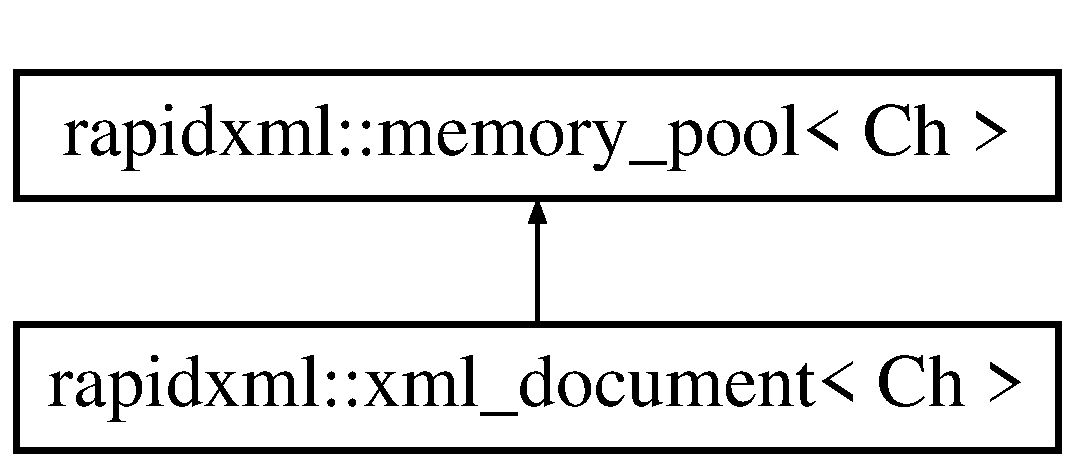
\includegraphics[height=2.000000cm]{classrapidxml_1_1memory__pool}
\end{center}
\end{figure}
\subsection*{Public Member Functions}
\begin{DoxyCompactItemize}
\item 
\hyperlink{classrapidxml_1_1memory__pool_a0b609da81dff28a19ebd704400788429}{memory\+\_\+pool} ()
\begin{DoxyCompactList}\small\item\em Constructs empty pool with default allocator functions. \end{DoxyCompactList}\item 
\hyperlink{classrapidxml_1_1memory__pool_a0a3e82126e59e4077f41e933130bb5a0}{$\sim$memory\+\_\+pool} ()
\item 
\hyperlink{classrapidxml_1_1xml__node}{xml\+\_\+node}$<$ Ch $>$ $\ast$ \hyperlink{classrapidxml_1_1memory__pool_a4118581c29ee9a2f6b55ebf7dac185f8}{allocate\+\_\+node} (\hyperlink{namespacerapidxml_abb456db38f7efb746c4330eed6072a7c}{node\+\_\+type} type, const Ch $\ast$name=0, const Ch $\ast$value=0, std\+::size\+\_\+t name\+\_\+size=0, std\+::size\+\_\+t value\+\_\+size=0)
\item 
\hyperlink{classrapidxml_1_1xml__attribute}{xml\+\_\+attribute}$<$ Ch $>$ $\ast$ \hyperlink{classrapidxml_1_1memory__pool_a3de2a66c983336e006ea3844e244ed30}{allocate\+\_\+attribute} (const Ch $\ast$name=0, const Ch $\ast$value=0, std\+::size\+\_\+t name\+\_\+size=0, std\+::size\+\_\+t value\+\_\+size=0)
\item 
Ch $\ast$ \hyperlink{classrapidxml_1_1memory__pool_a171941b39d55b868358da97462185f58}{allocate\+\_\+string} (const Ch $\ast$source=0, std\+::size\+\_\+t size=0)
\item 
\hyperlink{classrapidxml_1_1xml__node}{xml\+\_\+node}$<$ Ch $>$ $\ast$ \hyperlink{classrapidxml_1_1memory__pool_a0a10679fc17597d339a0dc107f8a94ac}{clone\+\_\+node} (const \hyperlink{classrapidxml_1_1xml__node}{xml\+\_\+node}$<$ Ch $>$ $\ast$source, \hyperlink{classrapidxml_1_1xml__node}{xml\+\_\+node}$<$ Ch $>$ $\ast$result=0)
\item 
void \hyperlink{classrapidxml_1_1memory__pool_aad377c835fdaed1cb2cc9df194cf84e4}{clear} ()
\item 
void \hyperlink{classrapidxml_1_1memory__pool_a84d3d8d2cdfc00501e1dcf26d889ae03}{set\+\_\+allocator} (alloc\+\_\+func $\ast$af, free\+\_\+func $\ast$ff)
\end{DoxyCompactItemize}


\subsection{Detailed Description}
\subsubsection*{template$<$class Ch = char$>$class rapidxml\+::memory\+\_\+pool$<$ Ch $>$}

This class is used by the parser to create new nodes and attributes, without overheads of dynamic memory allocation. 

This class is used by the parser to create new nodes and attributes, without overheads of dynamic memory allocation. In most cases, you will not need to use this class directly. However, if you need to create nodes manually or modify names/values of nodes, you are encouraged to use \hyperlink{classrapidxml_1_1memory__pool}{memory\+\_\+pool} of relevant \hyperlink{classrapidxml_1_1xml__document}{xml\+\_\+document} to allocate the memory. Not only is this faster than allocating them by using {\ttfamily new} operator, but also their lifetime will be tied to the lifetime of document, possibly simplyfing memory management. ~\newline
~\newline
 Call \hyperlink{classrapidxml_1_1memory__pool_a4118581c29ee9a2f6b55ebf7dac185f8}{allocate\+\_\+node()} or \hyperlink{classrapidxml_1_1memory__pool_a3de2a66c983336e006ea3844e244ed30}{allocate\+\_\+attribute()} functions to obtain new nodes or attributes from the pool. You can also call \hyperlink{classrapidxml_1_1memory__pool_a171941b39d55b868358da97462185f58}{allocate\+\_\+string()} function to allocate strings. Such strings can then be used as names or values of nodes without worrying about their lifetime. Note that there is no {\ttfamily free()} function -- all allocations are freed at once when \hyperlink{classrapidxml_1_1memory__pool_aad377c835fdaed1cb2cc9df194cf84e4}{clear()} function is called, or when the pool is destroyed. ~\newline
~\newline
 It is also possible to create a standalone \hyperlink{classrapidxml_1_1memory__pool}{memory\+\_\+pool}, and use it to allocate nodes, whose lifetime will not be tied to any document. ~\newline
~\newline
 Pool maintains {\ttfamily R\+A\+P\+I\+D\+X\+M\+L\+\_\+\+S\+T\+A\+T\+I\+C\+\_\+\+P\+O\+O\+L\+\_\+\+S\+I\+Z\+E} bytes of statically allocated memory. Until static memory is exhausted, no dynamic memory allocations are done. When static memory is exhausted, pool allocates additional blocks of memory of size {\ttfamily R\+A\+P\+I\+D\+X\+M\+L\+\_\+\+D\+Y\+N\+A\+M\+I\+C\+\_\+\+P\+O\+O\+L\+\_\+\+S\+I\+Z\+E} each, by using global {\ttfamily new\mbox{[}\mbox{]}} and {\ttfamily delete\mbox{[}\mbox{]}} operators. This behaviour can be changed by setting custom allocation routines. Use \hyperlink{classrapidxml_1_1memory__pool_a84d3d8d2cdfc00501e1dcf26d889ae03}{set\+\_\+allocator()} function to set them. ~\newline
~\newline
 Allocations for nodes, attributes and strings are aligned at {\ttfamily R\+A\+P\+I\+D\+X\+M\+L\+\_\+\+A\+L\+I\+G\+N\+M\+E\+N\+T} bytes. This value defaults to the size of pointer on target architecture. ~\newline
~\newline
 To obtain absolutely top performance from the parser, it is important that all nodes are allocated from a single, contiguous block of memory. Otherwise, cache misses when jumping between two (or more) disjoint blocks of memory can slow down parsing quite considerably. If required, you can tweak {\ttfamily R\+A\+P\+I\+D\+X\+M\+L\+\_\+\+S\+T\+A\+T\+I\+C\+\_\+\+P\+O\+O\+L\+\_\+\+S\+I\+Z\+E}, {\ttfamily R\+A\+P\+I\+D\+X\+M\+L\+\_\+\+D\+Y\+N\+A\+M\+I\+C\+\_\+\+P\+O\+O\+L\+\_\+\+S\+I\+Z\+E} and {\ttfamily R\+A\+P\+I\+D\+X\+M\+L\+\_\+\+A\+L\+I\+G\+N\+M\+E\+N\+T} to obtain best wasted memory to performance compromise. To do it, define their values before \hyperlink{rapidxml_8hpp}{rapidxml.\+hpp} file is included. 
\begin{DoxyParams}{Parameters}
{\em Ch} & Character type of created nodes. \\
\hline
\end{DoxyParams}


\subsection{Constructor \& Destructor Documentation}
\hypertarget{classrapidxml_1_1memory__pool_a0b609da81dff28a19ebd704400788429}{}\index{rapidxml\+::memory\+\_\+pool@{rapidxml\+::memory\+\_\+pool}!memory\+\_\+pool@{memory\+\_\+pool}}
\index{memory\+\_\+pool@{memory\+\_\+pool}!rapidxml\+::memory\+\_\+pool@{rapidxml\+::memory\+\_\+pool}}
\subsubsection[{memory\+\_\+pool()}]{\setlength{\rightskip}{0pt plus 5cm}template$<$class Ch  = char$>$ {\bf rapidxml\+::memory\+\_\+pool}$<$ Ch $>$\+::{\bf memory\+\_\+pool} (
\begin{DoxyParamCaption}
{}
\end{DoxyParamCaption}
)\hspace{0.3cm}{\ttfamily [inline]}}\label{classrapidxml_1_1memory__pool_a0b609da81dff28a19ebd704400788429}


Constructs empty pool with default allocator functions. 

\hypertarget{classrapidxml_1_1memory__pool_a0a3e82126e59e4077f41e933130bb5a0}{}\index{rapidxml\+::memory\+\_\+pool@{rapidxml\+::memory\+\_\+pool}!````~memory\+\_\+pool@{$\sim$memory\+\_\+pool}}
\index{````~memory\+\_\+pool@{$\sim$memory\+\_\+pool}!rapidxml\+::memory\+\_\+pool@{rapidxml\+::memory\+\_\+pool}}
\subsubsection[{$\sim$memory\+\_\+pool()}]{\setlength{\rightskip}{0pt plus 5cm}template$<$class Ch  = char$>$ {\bf rapidxml\+::memory\+\_\+pool}$<$ Ch $>$\+::$\sim${\bf memory\+\_\+pool} (
\begin{DoxyParamCaption}
{}
\end{DoxyParamCaption}
)\hspace{0.3cm}{\ttfamily [inline]}}\label{classrapidxml_1_1memory__pool_a0a3e82126e59e4077f41e933130bb5a0}
Destroys pool and frees all the memory. This causes memory occupied by nodes allocated by the pool to be freed. Nodes allocated from the pool are no longer valid. 

\subsection{Member Function Documentation}
\hypertarget{classrapidxml_1_1memory__pool_a3de2a66c983336e006ea3844e244ed30}{}\index{rapidxml\+::memory\+\_\+pool@{rapidxml\+::memory\+\_\+pool}!allocate\+\_\+attribute@{allocate\+\_\+attribute}}
\index{allocate\+\_\+attribute@{allocate\+\_\+attribute}!rapidxml\+::memory\+\_\+pool@{rapidxml\+::memory\+\_\+pool}}
\subsubsection[{allocate\+\_\+attribute(const Ch $\ast$name=0, const Ch $\ast$value=0, std\+::size\+\_\+t name\+\_\+size=0, std\+::size\+\_\+t value\+\_\+size=0)}]{\setlength{\rightskip}{0pt plus 5cm}template$<$class Ch  = char$>$ {\bf xml\+\_\+attribute}$<$Ch$>$$\ast$ {\bf rapidxml\+::memory\+\_\+pool}$<$ Ch $>$\+::allocate\+\_\+attribute (
\begin{DoxyParamCaption}
\item[{const Ch $\ast$}]{name = {\ttfamily 0}, }
\item[{const Ch $\ast$}]{value = {\ttfamily 0}, }
\item[{std\+::size\+\_\+t}]{name\+\_\+size = {\ttfamily 0}, }
\item[{std\+::size\+\_\+t}]{value\+\_\+size = {\ttfamily 0}}
\end{DoxyParamCaption}
)\hspace{0.3cm}{\ttfamily [inline]}}\label{classrapidxml_1_1memory__pool_a3de2a66c983336e006ea3844e244ed30}
Allocates a new attribute from the pool, and optionally assigns name and value to it. If the allocation request cannot be accomodated, this function will throw {\ttfamily std\+::bad\+\_\+alloc}. If exceptions are disabled by defining R\+A\+P\+I\+D\+X\+M\+L\+\_\+\+N\+O\+\_\+\+E\+X\+C\+E\+P\+T\+I\+O\+N\+S, this function will call rapidxml\+::parse\+\_\+error\+\_\+handler() function. 
\begin{DoxyParams}{Parameters}
{\em name} & Name to assign to the attribute, or 0 to assign no name. \\
\hline
{\em value} & Value to assign to the attribute, or 0 to assign no value. \\
\hline
{\em name\+\_\+size} & Size of name to assign, or 0 to automatically calculate size from name string. \\
\hline
{\em value\+\_\+size} & Size of value to assign, or 0 to automatically calculate size from value string. \\
\hline
\end{DoxyParams}
\begin{DoxyReturn}{Returns}
Pointer to allocated attribute. This pointer will never be N\+U\+L\+L. 
\end{DoxyReturn}
\hypertarget{classrapidxml_1_1memory__pool_a4118581c29ee9a2f6b55ebf7dac185f8}{}\index{rapidxml\+::memory\+\_\+pool@{rapidxml\+::memory\+\_\+pool}!allocate\+\_\+node@{allocate\+\_\+node}}
\index{allocate\+\_\+node@{allocate\+\_\+node}!rapidxml\+::memory\+\_\+pool@{rapidxml\+::memory\+\_\+pool}}
\subsubsection[{allocate\+\_\+node(node\+\_\+type type, const Ch $\ast$name=0, const Ch $\ast$value=0, std\+::size\+\_\+t name\+\_\+size=0, std\+::size\+\_\+t value\+\_\+size=0)}]{\setlength{\rightskip}{0pt plus 5cm}template$<$class Ch  = char$>$ {\bf xml\+\_\+node}$<$Ch$>$$\ast$ {\bf rapidxml\+::memory\+\_\+pool}$<$ Ch $>$\+::allocate\+\_\+node (
\begin{DoxyParamCaption}
\item[{{\bf node\+\_\+type}}]{type, }
\item[{const Ch $\ast$}]{name = {\ttfamily 0}, }
\item[{const Ch $\ast$}]{value = {\ttfamily 0}, }
\item[{std\+::size\+\_\+t}]{name\+\_\+size = {\ttfamily 0}, }
\item[{std\+::size\+\_\+t}]{value\+\_\+size = {\ttfamily 0}}
\end{DoxyParamCaption}
)\hspace{0.3cm}{\ttfamily [inline]}}\label{classrapidxml_1_1memory__pool_a4118581c29ee9a2f6b55ebf7dac185f8}
Allocates a new node from the pool, and optionally assigns name and value to it. If the allocation request cannot be accomodated, this function will throw {\ttfamily std\+::bad\+\_\+alloc}. If exceptions are disabled by defining R\+A\+P\+I\+D\+X\+M\+L\+\_\+\+N\+O\+\_\+\+E\+X\+C\+E\+P\+T\+I\+O\+N\+S, this function will call rapidxml\+::parse\+\_\+error\+\_\+handler() function. 
\begin{DoxyParams}{Parameters}
{\em type} & Type of node to create. \\
\hline
{\em name} & Name to assign to the node, or 0 to assign no name. \\
\hline
{\em value} & Value to assign to the node, or 0 to assign no value. \\
\hline
{\em name\+\_\+size} & Size of name to assign, or 0 to automatically calculate size from name string. \\
\hline
{\em value\+\_\+size} & Size of value to assign, or 0 to automatically calculate size from value string. \\
\hline
\end{DoxyParams}
\begin{DoxyReturn}{Returns}
Pointer to allocated node. This pointer will never be N\+U\+L\+L. 
\end{DoxyReturn}
\hypertarget{classrapidxml_1_1memory__pool_a171941b39d55b868358da97462185f58}{}\index{rapidxml\+::memory\+\_\+pool@{rapidxml\+::memory\+\_\+pool}!allocate\+\_\+string@{allocate\+\_\+string}}
\index{allocate\+\_\+string@{allocate\+\_\+string}!rapidxml\+::memory\+\_\+pool@{rapidxml\+::memory\+\_\+pool}}
\subsubsection[{allocate\+\_\+string(const Ch $\ast$source=0, std\+::size\+\_\+t size=0)}]{\setlength{\rightskip}{0pt plus 5cm}template$<$class Ch  = char$>$ Ch$\ast$ {\bf rapidxml\+::memory\+\_\+pool}$<$ Ch $>$\+::allocate\+\_\+string (
\begin{DoxyParamCaption}
\item[{const Ch $\ast$}]{source = {\ttfamily 0}, }
\item[{std\+::size\+\_\+t}]{size = {\ttfamily 0}}
\end{DoxyParamCaption}
)\hspace{0.3cm}{\ttfamily [inline]}}\label{classrapidxml_1_1memory__pool_a171941b39d55b868358da97462185f58}
Allocates a char array of given size from the pool, and optionally copies a given string to it. If the allocation request cannot be accomodated, this function will throw {\ttfamily std\+::bad\+\_\+alloc}. If exceptions are disabled by defining R\+A\+P\+I\+D\+X\+M\+L\+\_\+\+N\+O\+\_\+\+E\+X\+C\+E\+P\+T\+I\+O\+N\+S, this function will call rapidxml\+::parse\+\_\+error\+\_\+handler() function. 
\begin{DoxyParams}{Parameters}
{\em source} & String to initialize the allocated memory with, or 0 to not initialize it. \\
\hline
{\em size} & Number of characters to allocate, or zero to calculate it automatically from source string length; if size is 0, source string must be specified and null terminated. \\
\hline
\end{DoxyParams}
\begin{DoxyReturn}{Returns}
Pointer to allocated char array. This pointer will never be N\+U\+L\+L. 
\end{DoxyReturn}
\hypertarget{classrapidxml_1_1memory__pool_aad377c835fdaed1cb2cc9df194cf84e4}{}\index{rapidxml\+::memory\+\_\+pool@{rapidxml\+::memory\+\_\+pool}!clear@{clear}}
\index{clear@{clear}!rapidxml\+::memory\+\_\+pool@{rapidxml\+::memory\+\_\+pool}}
\subsubsection[{clear()}]{\setlength{\rightskip}{0pt plus 5cm}template$<$class Ch  = char$>$ void {\bf rapidxml\+::memory\+\_\+pool}$<$ Ch $>$\+::clear (
\begin{DoxyParamCaption}
{}
\end{DoxyParamCaption}
)\hspace{0.3cm}{\ttfamily [inline]}}\label{classrapidxml_1_1memory__pool_aad377c835fdaed1cb2cc9df194cf84e4}
Clears the pool. This causes memory occupied by nodes allocated by the pool to be freed. Any nodes or strings allocated from the pool will no longer be valid. \hypertarget{classrapidxml_1_1memory__pool_a0a10679fc17597d339a0dc107f8a94ac}{}\index{rapidxml\+::memory\+\_\+pool@{rapidxml\+::memory\+\_\+pool}!clone\+\_\+node@{clone\+\_\+node}}
\index{clone\+\_\+node@{clone\+\_\+node}!rapidxml\+::memory\+\_\+pool@{rapidxml\+::memory\+\_\+pool}}
\subsubsection[{clone\+\_\+node(const xml\+\_\+node$<$ Ch $>$ $\ast$source, xml\+\_\+node$<$ Ch $>$ $\ast$result=0)}]{\setlength{\rightskip}{0pt plus 5cm}template$<$class Ch  = char$>$ {\bf xml\+\_\+node}$<$Ch$>$$\ast$ {\bf rapidxml\+::memory\+\_\+pool}$<$ Ch $>$\+::clone\+\_\+node (
\begin{DoxyParamCaption}
\item[{const {\bf xml\+\_\+node}$<$ Ch $>$ $\ast$}]{source, }
\item[{{\bf xml\+\_\+node}$<$ Ch $>$ $\ast$}]{result = {\ttfamily 0}}
\end{DoxyParamCaption}
)\hspace{0.3cm}{\ttfamily [inline]}}\label{classrapidxml_1_1memory__pool_a0a10679fc17597d339a0dc107f8a94ac}
Clones an \hyperlink{classrapidxml_1_1xml__node}{xml\+\_\+node} and its hierarchy of child nodes and attributes. Nodes and attributes are allocated from this memory pool. Names and values are not cloned, they are shared between the clone and the source. Result node can be optionally specified as a second parameter, in which case its contents will be replaced with cloned source node. This is useful when you want to clone entire document. 
\begin{DoxyParams}{Parameters}
{\em source} & Node to clone. \\
\hline
{\em result} & Node to put results in, or 0 to automatically allocate result node \\
\hline
\end{DoxyParams}
\begin{DoxyReturn}{Returns}
Pointer to cloned node. This pointer will never be N\+U\+L\+L. 
\end{DoxyReturn}
\hypertarget{classrapidxml_1_1memory__pool_a84d3d8d2cdfc00501e1dcf26d889ae03}{}\index{rapidxml\+::memory\+\_\+pool@{rapidxml\+::memory\+\_\+pool}!set\+\_\+allocator@{set\+\_\+allocator}}
\index{set\+\_\+allocator@{set\+\_\+allocator}!rapidxml\+::memory\+\_\+pool@{rapidxml\+::memory\+\_\+pool}}
\subsubsection[{set\+\_\+allocator(alloc\+\_\+func $\ast$af, free\+\_\+func $\ast$ff)}]{\setlength{\rightskip}{0pt plus 5cm}template$<$class Ch  = char$>$ void {\bf rapidxml\+::memory\+\_\+pool}$<$ Ch $>$\+::set\+\_\+allocator (
\begin{DoxyParamCaption}
\item[{alloc\+\_\+func $\ast$}]{af, }
\item[{free\+\_\+func $\ast$}]{ff}
\end{DoxyParamCaption}
)\hspace{0.3cm}{\ttfamily [inline]}}\label{classrapidxml_1_1memory__pool_a84d3d8d2cdfc00501e1dcf26d889ae03}
Sets or resets the user-\/defined memory allocation functions for the pool. This can only be called when no memory is allocated from the pool yet, otherwise results are undefined. Allocation function must not return invalid pointer on failure. It should either throw, stop the program, or use {\ttfamily longjmp()} function to pass control to other place of program. If it returns invalid pointer, results are undefined. ~\newline
~\newline
 User defined allocation functions must have the following forms\+: ~\newline
{\ttfamily  ~\newline
void $\ast$allocate(std\+::size\+\_\+t size); ~\newline
void free(void $\ast$pointer); }~\newline
 
\begin{DoxyParams}{Parameters}
{\em af} & Allocation function, or 0 to restore default function \\
\hline
{\em ff} & Free function, or 0 to restore default function \\
\hline
\end{DoxyParams}


The documentation for this class was generated from the following file\+:\begin{DoxyCompactItemize}
\item 
/\+Users/brandonmcfarland/\+Desktop/searchdocs/\+Search\+Engine/\+Final\+Project/\hyperlink{rapidxml_8hpp}{rapidxml.\+hpp}\end{DoxyCompactItemize}

\hypertarget{classrapidxml_1_1node__iterator}{}\section{rapidxml\+:\+:node\+\_\+iterator$<$ Ch $>$ Class Template Reference}
\label{classrapidxml_1_1node__iterator}\index{rapidxml\+::node\+\_\+iterator$<$ Ch $>$@{rapidxml\+::node\+\_\+iterator$<$ Ch $>$}}


Iterator of child nodes of \hyperlink{classrapidxml_1_1xml__node}{xml\+\_\+node}.  




{\ttfamily \#include $<$rapidxml\+\_\+iterators.\+hpp$>$}

\subsection*{Public Types}
\begin{DoxyCompactItemize}
\item 
typedef \hyperlink{classrapidxml_1_1xml__node}{xml\+\_\+node}$<$ Ch $>$ \hyperlink{classrapidxml_1_1node__iterator_ade6310119ed1f72c94830e006fac69b7}{value\+\_\+type}
\item 
typedef \hyperlink{classrapidxml_1_1xml__node}{xml\+\_\+node}$<$ Ch $>$ \& \hyperlink{classrapidxml_1_1node__iterator_ad7fabbcb7d3d9e4e220299c5475b9e9c}{reference}
\item 
typedef \hyperlink{classrapidxml_1_1xml__node}{xml\+\_\+node}$<$ Ch $>$ $\ast$ \hyperlink{classrapidxml_1_1node__iterator_a65dca8bca2b9c29f635b9ad0bdeeecb9}{pointer}
\item 
typedef std\+::ptrdiff\+\_\+t \hyperlink{classrapidxml_1_1node__iterator_a5bdc462b980a52c5fa2d99ac9f4f4bff}{difference\+\_\+type}
\item 
typedef std\+::bidirectional\+\_\+iterator\+\_\+tag \hyperlink{classrapidxml_1_1node__iterator_a8e82d75f768e17bf7349d010ee26c037}{iterator\+\_\+category}
\end{DoxyCompactItemize}
\subsection*{Public Member Functions}
\begin{DoxyCompactItemize}
\item 
\hyperlink{classrapidxml_1_1node__iterator_a4e1244b9e9e1d2b5129235806d1e31ad}{node\+\_\+iterator} ()
\item 
\hyperlink{classrapidxml_1_1node__iterator_a94c3da59b54e4bd003e226cc35b3c266}{node\+\_\+iterator} (\hyperlink{classrapidxml_1_1xml__node}{xml\+\_\+node}$<$ Ch $>$ $\ast$node)
\item 
\hyperlink{classrapidxml_1_1node__iterator_ad7fabbcb7d3d9e4e220299c5475b9e9c}{reference} \hyperlink{classrapidxml_1_1node__iterator_ab31fe5bc1fd01fee8a2b31c3e42d78ed}{operator$\ast$} () const 
\item 
\hyperlink{classrapidxml_1_1node__iterator_a65dca8bca2b9c29f635b9ad0bdeeecb9}{pointer} \hyperlink{classrapidxml_1_1node__iterator_a9b3e7d58c4a628524914932e0663ddfb}{operator-\/$>$} () const 
\item 
\hyperlink{classrapidxml_1_1node__iterator}{node\+\_\+iterator} \& \hyperlink{classrapidxml_1_1node__iterator_a8d6b184a76b2ec8a8b5e90bc013c80ed}{operator++} ()
\item 
\hyperlink{classrapidxml_1_1node__iterator}{node\+\_\+iterator} \hyperlink{classrapidxml_1_1node__iterator_ad01b4e43e348a330984833fd4924d0f2}{operator++} (int)
\item 
\hyperlink{classrapidxml_1_1node__iterator}{node\+\_\+iterator} \& \hyperlink{classrapidxml_1_1node__iterator_ace52107ecd1bcf02e49619e86206e3a3}{operator-\/-\/} ()
\item 
\hyperlink{classrapidxml_1_1node__iterator}{node\+\_\+iterator} \hyperlink{classrapidxml_1_1node__iterator_a4ca35716bb7865f199a137b063af6080}{operator-\/-\/} (int)
\item 
bool \hyperlink{classrapidxml_1_1node__iterator_a5cb8a3b0d65a1a2517995e986a4debfd}{operator==} (const \hyperlink{classrapidxml_1_1node__iterator}{node\+\_\+iterator}$<$ Ch $>$ \&rhs)
\item 
bool \hyperlink{classrapidxml_1_1node__iterator_a20f1e25347d7e3856694f18597f7c8e2}{operator!=} (const \hyperlink{classrapidxml_1_1node__iterator}{node\+\_\+iterator}$<$ Ch $>$ \&rhs)
\end{DoxyCompactItemize}


\subsection{Detailed Description}
\subsubsection*{template$<$class Ch$>$class rapidxml\+::node\+\_\+iterator$<$ Ch $>$}

Iterator of child nodes of \hyperlink{classrapidxml_1_1xml__node}{xml\+\_\+node}. 

\subsection{Member Typedef Documentation}
\hypertarget{classrapidxml_1_1node__iterator_a5bdc462b980a52c5fa2d99ac9f4f4bff}{}\index{rapidxml\+::node\+\_\+iterator@{rapidxml\+::node\+\_\+iterator}!difference\+\_\+type@{difference\+\_\+type}}
\index{difference\+\_\+type@{difference\+\_\+type}!rapidxml\+::node\+\_\+iterator@{rapidxml\+::node\+\_\+iterator}}
\subsubsection[{difference\+\_\+type}]{\setlength{\rightskip}{0pt plus 5cm}template$<$class Ch$>$ typedef std\+::ptrdiff\+\_\+t {\bf rapidxml\+::node\+\_\+iterator}$<$ Ch $>$\+::{\bf difference\+\_\+type}}\label{classrapidxml_1_1node__iterator_a5bdc462b980a52c5fa2d99ac9f4f4bff}
\hypertarget{classrapidxml_1_1node__iterator_a8e82d75f768e17bf7349d010ee26c037}{}\index{rapidxml\+::node\+\_\+iterator@{rapidxml\+::node\+\_\+iterator}!iterator\+\_\+category@{iterator\+\_\+category}}
\index{iterator\+\_\+category@{iterator\+\_\+category}!rapidxml\+::node\+\_\+iterator@{rapidxml\+::node\+\_\+iterator}}
\subsubsection[{iterator\+\_\+category}]{\setlength{\rightskip}{0pt plus 5cm}template$<$class Ch$>$ typedef std\+::bidirectional\+\_\+iterator\+\_\+tag {\bf rapidxml\+::node\+\_\+iterator}$<$ Ch $>$\+::{\bf iterator\+\_\+category}}\label{classrapidxml_1_1node__iterator_a8e82d75f768e17bf7349d010ee26c037}
\hypertarget{classrapidxml_1_1node__iterator_a65dca8bca2b9c29f635b9ad0bdeeecb9}{}\index{rapidxml\+::node\+\_\+iterator@{rapidxml\+::node\+\_\+iterator}!pointer@{pointer}}
\index{pointer@{pointer}!rapidxml\+::node\+\_\+iterator@{rapidxml\+::node\+\_\+iterator}}
\subsubsection[{pointer}]{\setlength{\rightskip}{0pt plus 5cm}template$<$class Ch$>$ typedef {\bf xml\+\_\+node}$<$Ch$>$$\ast$ {\bf rapidxml\+::node\+\_\+iterator}$<$ Ch $>$\+::{\bf pointer}}\label{classrapidxml_1_1node__iterator_a65dca8bca2b9c29f635b9ad0bdeeecb9}
\hypertarget{classrapidxml_1_1node__iterator_ad7fabbcb7d3d9e4e220299c5475b9e9c}{}\index{rapidxml\+::node\+\_\+iterator@{rapidxml\+::node\+\_\+iterator}!reference@{reference}}
\index{reference@{reference}!rapidxml\+::node\+\_\+iterator@{rapidxml\+::node\+\_\+iterator}}
\subsubsection[{reference}]{\setlength{\rightskip}{0pt plus 5cm}template$<$class Ch$>$ typedef {\bf xml\+\_\+node}$<$Ch$>$\& {\bf rapidxml\+::node\+\_\+iterator}$<$ Ch $>$\+::{\bf reference}}\label{classrapidxml_1_1node__iterator_ad7fabbcb7d3d9e4e220299c5475b9e9c}
\hypertarget{classrapidxml_1_1node__iterator_ade6310119ed1f72c94830e006fac69b7}{}\index{rapidxml\+::node\+\_\+iterator@{rapidxml\+::node\+\_\+iterator}!value\+\_\+type@{value\+\_\+type}}
\index{value\+\_\+type@{value\+\_\+type}!rapidxml\+::node\+\_\+iterator@{rapidxml\+::node\+\_\+iterator}}
\subsubsection[{value\+\_\+type}]{\setlength{\rightskip}{0pt plus 5cm}template$<$class Ch$>$ typedef {\bf xml\+\_\+node}$<$Ch$>$ {\bf rapidxml\+::node\+\_\+iterator}$<$ Ch $>$\+::{\bf value\+\_\+type}}\label{classrapidxml_1_1node__iterator_ade6310119ed1f72c94830e006fac69b7}


\subsection{Constructor \& Destructor Documentation}
\hypertarget{classrapidxml_1_1node__iterator_a4e1244b9e9e1d2b5129235806d1e31ad}{}\index{rapidxml\+::node\+\_\+iterator@{rapidxml\+::node\+\_\+iterator}!node\+\_\+iterator@{node\+\_\+iterator}}
\index{node\+\_\+iterator@{node\+\_\+iterator}!rapidxml\+::node\+\_\+iterator@{rapidxml\+::node\+\_\+iterator}}
\subsubsection[{node\+\_\+iterator()}]{\setlength{\rightskip}{0pt plus 5cm}template$<$class Ch$>$ {\bf rapidxml\+::node\+\_\+iterator}$<$ Ch $>$\+::{\bf node\+\_\+iterator} (
\begin{DoxyParamCaption}
{}
\end{DoxyParamCaption}
)\hspace{0.3cm}{\ttfamily [inline]}}\label{classrapidxml_1_1node__iterator_a4e1244b9e9e1d2b5129235806d1e31ad}
\hypertarget{classrapidxml_1_1node__iterator_a94c3da59b54e4bd003e226cc35b3c266}{}\index{rapidxml\+::node\+\_\+iterator@{rapidxml\+::node\+\_\+iterator}!node\+\_\+iterator@{node\+\_\+iterator}}
\index{node\+\_\+iterator@{node\+\_\+iterator}!rapidxml\+::node\+\_\+iterator@{rapidxml\+::node\+\_\+iterator}}
\subsubsection[{node\+\_\+iterator(xml\+\_\+node$<$ Ch $>$ $\ast$node)}]{\setlength{\rightskip}{0pt plus 5cm}template$<$class Ch$>$ {\bf rapidxml\+::node\+\_\+iterator}$<$ Ch $>$\+::{\bf node\+\_\+iterator} (
\begin{DoxyParamCaption}
\item[{{\bf xml\+\_\+node}$<$ Ch $>$ $\ast$}]{node}
\end{DoxyParamCaption}
)\hspace{0.3cm}{\ttfamily [inline]}}\label{classrapidxml_1_1node__iterator_a94c3da59b54e4bd003e226cc35b3c266}


\subsection{Member Function Documentation}
\hypertarget{classrapidxml_1_1node__iterator_a20f1e25347d7e3856694f18597f7c8e2}{}\index{rapidxml\+::node\+\_\+iterator@{rapidxml\+::node\+\_\+iterator}!operator"!=@{operator"!=}}
\index{operator"!=@{operator"!=}!rapidxml\+::node\+\_\+iterator@{rapidxml\+::node\+\_\+iterator}}
\subsubsection[{operator"!=(const node\+\_\+iterator$<$ Ch $>$ \&rhs)}]{\setlength{\rightskip}{0pt plus 5cm}template$<$class Ch$>$ bool {\bf rapidxml\+::node\+\_\+iterator}$<$ Ch $>$\+::operator!= (
\begin{DoxyParamCaption}
\item[{const {\bf node\+\_\+iterator}$<$ Ch $>$ \&}]{rhs}
\end{DoxyParamCaption}
)\hspace{0.3cm}{\ttfamily [inline]}}\label{classrapidxml_1_1node__iterator_a20f1e25347d7e3856694f18597f7c8e2}
\hypertarget{classrapidxml_1_1node__iterator_ab31fe5bc1fd01fee8a2b31c3e42d78ed}{}\index{rapidxml\+::node\+\_\+iterator@{rapidxml\+::node\+\_\+iterator}!operator$\ast$@{operator$\ast$}}
\index{operator$\ast$@{operator$\ast$}!rapidxml\+::node\+\_\+iterator@{rapidxml\+::node\+\_\+iterator}}
\subsubsection[{operator$\ast$() const }]{\setlength{\rightskip}{0pt plus 5cm}template$<$class Ch$>$ {\bf reference} {\bf rapidxml\+::node\+\_\+iterator}$<$ Ch $>$\+::operator$\ast$ (
\begin{DoxyParamCaption}
{}
\end{DoxyParamCaption}
) const\hspace{0.3cm}{\ttfamily [inline]}}\label{classrapidxml_1_1node__iterator_ab31fe5bc1fd01fee8a2b31c3e42d78ed}
\hypertarget{classrapidxml_1_1node__iterator_a8d6b184a76b2ec8a8b5e90bc013c80ed}{}\index{rapidxml\+::node\+\_\+iterator@{rapidxml\+::node\+\_\+iterator}!operator++@{operator++}}
\index{operator++@{operator++}!rapidxml\+::node\+\_\+iterator@{rapidxml\+::node\+\_\+iterator}}
\subsubsection[{operator++()}]{\setlength{\rightskip}{0pt plus 5cm}template$<$class Ch$>$ {\bf node\+\_\+iterator}\& {\bf rapidxml\+::node\+\_\+iterator}$<$ Ch $>$\+::operator++ (
\begin{DoxyParamCaption}
{}
\end{DoxyParamCaption}
)\hspace{0.3cm}{\ttfamily [inline]}}\label{classrapidxml_1_1node__iterator_a8d6b184a76b2ec8a8b5e90bc013c80ed}
\hypertarget{classrapidxml_1_1node__iterator_ad01b4e43e348a330984833fd4924d0f2}{}\index{rapidxml\+::node\+\_\+iterator@{rapidxml\+::node\+\_\+iterator}!operator++@{operator++}}
\index{operator++@{operator++}!rapidxml\+::node\+\_\+iterator@{rapidxml\+::node\+\_\+iterator}}
\subsubsection[{operator++(int)}]{\setlength{\rightskip}{0pt plus 5cm}template$<$class Ch$>$ {\bf node\+\_\+iterator} {\bf rapidxml\+::node\+\_\+iterator}$<$ Ch $>$\+::operator++ (
\begin{DoxyParamCaption}
\item[{int}]{}
\end{DoxyParamCaption}
)\hspace{0.3cm}{\ttfamily [inline]}}\label{classrapidxml_1_1node__iterator_ad01b4e43e348a330984833fd4924d0f2}
\hypertarget{classrapidxml_1_1node__iterator_ace52107ecd1bcf02e49619e86206e3a3}{}\index{rapidxml\+::node\+\_\+iterator@{rapidxml\+::node\+\_\+iterator}!operator-\/-\/@{operator-\/-\/}}
\index{operator-\/-\/@{operator-\/-\/}!rapidxml\+::node\+\_\+iterator@{rapidxml\+::node\+\_\+iterator}}
\subsubsection[{operator-\/-\/()}]{\setlength{\rightskip}{0pt plus 5cm}template$<$class Ch$>$ {\bf node\+\_\+iterator}\& {\bf rapidxml\+::node\+\_\+iterator}$<$ Ch $>$\+::operator-\/-\/ (
\begin{DoxyParamCaption}
{}
\end{DoxyParamCaption}
)\hspace{0.3cm}{\ttfamily [inline]}}\label{classrapidxml_1_1node__iterator_ace52107ecd1bcf02e49619e86206e3a3}
\hypertarget{classrapidxml_1_1node__iterator_a4ca35716bb7865f199a137b063af6080}{}\index{rapidxml\+::node\+\_\+iterator@{rapidxml\+::node\+\_\+iterator}!operator-\/-\/@{operator-\/-\/}}
\index{operator-\/-\/@{operator-\/-\/}!rapidxml\+::node\+\_\+iterator@{rapidxml\+::node\+\_\+iterator}}
\subsubsection[{operator-\/-\/(int)}]{\setlength{\rightskip}{0pt plus 5cm}template$<$class Ch$>$ {\bf node\+\_\+iterator} {\bf rapidxml\+::node\+\_\+iterator}$<$ Ch $>$\+::operator-\/-\/ (
\begin{DoxyParamCaption}
\item[{int}]{}
\end{DoxyParamCaption}
)\hspace{0.3cm}{\ttfamily [inline]}}\label{classrapidxml_1_1node__iterator_a4ca35716bb7865f199a137b063af6080}
\hypertarget{classrapidxml_1_1node__iterator_a9b3e7d58c4a628524914932e0663ddfb}{}\index{rapidxml\+::node\+\_\+iterator@{rapidxml\+::node\+\_\+iterator}!operator-\/$>$@{operator-\/$>$}}
\index{operator-\/$>$@{operator-\/$>$}!rapidxml\+::node\+\_\+iterator@{rapidxml\+::node\+\_\+iterator}}
\subsubsection[{operator-\/$>$() const }]{\setlength{\rightskip}{0pt plus 5cm}template$<$class Ch$>$ {\bf pointer} {\bf rapidxml\+::node\+\_\+iterator}$<$ Ch $>$\+::operator-\/$>$ (
\begin{DoxyParamCaption}
{}
\end{DoxyParamCaption}
) const\hspace{0.3cm}{\ttfamily [inline]}}\label{classrapidxml_1_1node__iterator_a9b3e7d58c4a628524914932e0663ddfb}
\hypertarget{classrapidxml_1_1node__iterator_a5cb8a3b0d65a1a2517995e986a4debfd}{}\index{rapidxml\+::node\+\_\+iterator@{rapidxml\+::node\+\_\+iterator}!operator==@{operator==}}
\index{operator==@{operator==}!rapidxml\+::node\+\_\+iterator@{rapidxml\+::node\+\_\+iterator}}
\subsubsection[{operator==(const node\+\_\+iterator$<$ Ch $>$ \&rhs)}]{\setlength{\rightskip}{0pt plus 5cm}template$<$class Ch$>$ bool {\bf rapidxml\+::node\+\_\+iterator}$<$ Ch $>$\+::operator== (
\begin{DoxyParamCaption}
\item[{const {\bf node\+\_\+iterator}$<$ Ch $>$ \&}]{rhs}
\end{DoxyParamCaption}
)\hspace{0.3cm}{\ttfamily [inline]}}\label{classrapidxml_1_1node__iterator_a5cb8a3b0d65a1a2517995e986a4debfd}


The documentation for this class was generated from the following file\+:\begin{DoxyCompactItemize}
\item 
/\+Users/brandonmcfarland/\+Desktop/searchdocs/\+Search\+Engine/\+Final\+Project/\hyperlink{rapidxml__iterators_8hpp}{rapidxml\+\_\+iterators.\+hpp}\end{DoxyCompactItemize}

\hypertarget{class_page_info}{}\section{Page\+Info Class Reference}
\label{class_page_info}\index{Page\+Info@{Page\+Info}}


In the inverted index, pages are assigned integer I\+Ds to improve performance. \hyperlink{class_page_info}{Page\+Info} objects hold the data corresponding with said I\+Ds.  




{\ttfamily \#include $<$pageinfo.\+h$>$}

\subsection*{Public Member Functions}
\begin{DoxyCompactItemize}
\item 
\hyperlink{class_page_info_a3ab3b93ca3b3d09645d5e187863b84e6}{Page\+Info} ()
\item 
\hyperlink{class_page_info_a45259793eed3f830dadecfde0e970ec5}{$\sim$\+Page\+Info} ()
\item 
\hyperlink{class_page_info_aa98a49dd45fdea434a27e4892dbdf032}{Page\+Info} (string the\+Content, string the\+Contributor, string the\+Timestamp, string the\+Title)
\begin{DoxyCompactList}\small\item\em The only constructor ever called. \end{DoxyCompactList}\item 
string \hyperlink{class_page_info_a61bd04fcecb67f3fac9833cd4a0e432b}{get\+\_\+content} ()
\begin{DoxyCompactList}\small\item\em Returns the content from \hyperlink{class_page_info}{Page\+Info}. \end{DoxyCompactList}\item 
string \hyperlink{class_page_info_a6569fb1fd2a7efa4a6d144aa87c27912}{get\+\_\+contributor} ()
\begin{DoxyCompactList}\small\item\em Returns contributor or I\+P address. \end{DoxyCompactList}\item 
string \hyperlink{class_page_info_ab2fa01ac638b965912b93fce36d4899a}{get\+\_\+timestamp} ()
\begin{DoxyCompactList}\small\item\em Returns the timestamp of the page. \end{DoxyCompactList}\item 
string \hyperlink{class_page_info_a0985d632ae64c913fe976bedccaf5d31}{get\+\_\+title} ()
\begin{DoxyCompactList}\small\item\em Returns the title of the page. \end{DoxyCompactList}\item 
int \hyperlink{class_page_info_a40938f3d2f1c81079abcbe8051143d53}{get\+\_\+total\+Words} ()
\begin{DoxyCompactList}\small\item\em Returns the total number of words of the page. \end{DoxyCompactList}\item 
void \hyperlink{class_page_info_afaf6005be3e5fa629619038a96fbd1af}{set\+\_\+content} (string the\+Content)
\begin{DoxyCompactList}\small\item\em Sets variable content to string the\+Content. \end{DoxyCompactList}\item 
void \hyperlink{class_page_info_afb03f9cd31ec6e6f500393cd5c7e1037}{set\+\_\+contributor} (string the\+Info)
\begin{DoxyCompactList}\small\item\em Sets variable contributon\+Name\+Oe\+I\+P to string the\+Info. \end{DoxyCompactList}\item 
void \hyperlink{class_page_info_ad8f8aada94adc772c9739f5dcb3223a7}{set\+\_\+timestamp} (string the\+Timestamp)
\begin{DoxyCompactList}\small\item\em Sets variable timestamp to string the\+Timestamp. \end{DoxyCompactList}\item 
void \hyperlink{class_page_info_a0808f61697bbeca2d717d9b55b233ae1}{set\+\_\+title} (string the\+Title)
\begin{DoxyCompactList}\small\item\em Sets variable title to string the\+Title. \end{DoxyCompactList}\item 
void \hyperlink{class_page_info_adcd293f9d6bdc291f7f28663e7151c45}{set\+\_\+total\+Words} (int the\+Total)
\begin{DoxyCompactList}\small\item\em Sets variable total\+Words to string the\+Total. \end{DoxyCompactList}\item 
void \hyperlink{class_page_info_a43de865e72ac2fc61f124e2acee9da4d}{incr\+\_\+total\+Words} (int incr)
\begin{DoxyCompactList}\small\item\em Increment total\+Words by a given value. \end{DoxyCompactList}\end{DoxyCompactItemize}


\subsection{Detailed Description}
In the inverted index, pages are assigned integer I\+Ds to improve performance. \hyperlink{class_page_info}{Page\+Info} objects hold the data corresponding with said I\+Ds. 

\subsection{Constructor \& Destructor Documentation}
\hypertarget{class_page_info_a3ab3b93ca3b3d09645d5e187863b84e6}{}\index{Page\+Info@{Page\+Info}!Page\+Info@{Page\+Info}}
\index{Page\+Info@{Page\+Info}!Page\+Info@{Page\+Info}}
\subsubsection[{Page\+Info()}]{\setlength{\rightskip}{0pt plus 5cm}Page\+Info\+::\+Page\+Info (
\begin{DoxyParamCaption}
{}
\end{DoxyParamCaption}
)}\label{class_page_info_a3ab3b93ca3b3d09645d5e187863b84e6}
\hypertarget{class_page_info_a45259793eed3f830dadecfde0e970ec5}{}\index{Page\+Info@{Page\+Info}!````~Page\+Info@{$\sim$\+Page\+Info}}
\index{````~Page\+Info@{$\sim$\+Page\+Info}!Page\+Info@{Page\+Info}}
\subsubsection[{$\sim$\+Page\+Info()}]{\setlength{\rightskip}{0pt plus 5cm}Page\+Info\+::$\sim$\+Page\+Info (
\begin{DoxyParamCaption}
{}
\end{DoxyParamCaption}
)}\label{class_page_info_a45259793eed3f830dadecfde0e970ec5}
\hypertarget{class_page_info_aa98a49dd45fdea434a27e4892dbdf032}{}\index{Page\+Info@{Page\+Info}!Page\+Info@{Page\+Info}}
\index{Page\+Info@{Page\+Info}!Page\+Info@{Page\+Info}}
\subsubsection[{Page\+Info(string the\+Content, string the\+Contributor, string the\+Timestamp, string the\+Title)}]{\setlength{\rightskip}{0pt plus 5cm}Page\+Info\+::\+Page\+Info (
\begin{DoxyParamCaption}
\item[{string}]{the\+Content, }
\item[{string}]{the\+Contributor, }
\item[{string}]{the\+Timestamp, }
\item[{string}]{the\+Title}
\end{DoxyParamCaption}
)}\label{class_page_info_aa98a49dd45fdea434a27e4892dbdf032}


The only constructor ever called. 



\subsection{Member Function Documentation}
\hypertarget{class_page_info_a61bd04fcecb67f3fac9833cd4a0e432b}{}\index{Page\+Info@{Page\+Info}!get\+\_\+content@{get\+\_\+content}}
\index{get\+\_\+content@{get\+\_\+content}!Page\+Info@{Page\+Info}}
\subsubsection[{get\+\_\+content()}]{\setlength{\rightskip}{0pt plus 5cm}string Page\+Info\+::get\+\_\+content (
\begin{DoxyParamCaption}
{}
\end{DoxyParamCaption}
)}\label{class_page_info_a61bd04fcecb67f3fac9833cd4a0e432b}


Returns the content from \hyperlink{class_page_info}{Page\+Info}. 

\hypertarget{class_page_info_a6569fb1fd2a7efa4a6d144aa87c27912}{}\index{Page\+Info@{Page\+Info}!get\+\_\+contributor@{get\+\_\+contributor}}
\index{get\+\_\+contributor@{get\+\_\+contributor}!Page\+Info@{Page\+Info}}
\subsubsection[{get\+\_\+contributor()}]{\setlength{\rightskip}{0pt plus 5cm}string Page\+Info\+::get\+\_\+contributor (
\begin{DoxyParamCaption}
{}
\end{DoxyParamCaption}
)}\label{class_page_info_a6569fb1fd2a7efa4a6d144aa87c27912}


Returns contributor or I\+P address. 

\hypertarget{class_page_info_ab2fa01ac638b965912b93fce36d4899a}{}\index{Page\+Info@{Page\+Info}!get\+\_\+timestamp@{get\+\_\+timestamp}}
\index{get\+\_\+timestamp@{get\+\_\+timestamp}!Page\+Info@{Page\+Info}}
\subsubsection[{get\+\_\+timestamp()}]{\setlength{\rightskip}{0pt plus 5cm}string Page\+Info\+::get\+\_\+timestamp (
\begin{DoxyParamCaption}
{}
\end{DoxyParamCaption}
)}\label{class_page_info_ab2fa01ac638b965912b93fce36d4899a}


Returns the timestamp of the page. 

\hypertarget{class_page_info_a0985d632ae64c913fe976bedccaf5d31}{}\index{Page\+Info@{Page\+Info}!get\+\_\+title@{get\+\_\+title}}
\index{get\+\_\+title@{get\+\_\+title}!Page\+Info@{Page\+Info}}
\subsubsection[{get\+\_\+title()}]{\setlength{\rightskip}{0pt plus 5cm}string Page\+Info\+::get\+\_\+title (
\begin{DoxyParamCaption}
{}
\end{DoxyParamCaption}
)}\label{class_page_info_a0985d632ae64c913fe976bedccaf5d31}


Returns the title of the page. 

\hypertarget{class_page_info_a40938f3d2f1c81079abcbe8051143d53}{}\index{Page\+Info@{Page\+Info}!get\+\_\+total\+Words@{get\+\_\+total\+Words}}
\index{get\+\_\+total\+Words@{get\+\_\+total\+Words}!Page\+Info@{Page\+Info}}
\subsubsection[{get\+\_\+total\+Words()}]{\setlength{\rightskip}{0pt plus 5cm}int Page\+Info\+::get\+\_\+total\+Words (
\begin{DoxyParamCaption}
{}
\end{DoxyParamCaption}
)}\label{class_page_info_a40938f3d2f1c81079abcbe8051143d53}


Returns the total number of words of the page. 

\hypertarget{class_page_info_a43de865e72ac2fc61f124e2acee9da4d}{}\index{Page\+Info@{Page\+Info}!incr\+\_\+total\+Words@{incr\+\_\+total\+Words}}
\index{incr\+\_\+total\+Words@{incr\+\_\+total\+Words}!Page\+Info@{Page\+Info}}
\subsubsection[{incr\+\_\+total\+Words(int incr)}]{\setlength{\rightskip}{0pt plus 5cm}void Page\+Info\+::incr\+\_\+total\+Words (
\begin{DoxyParamCaption}
\item[{int}]{incr}
\end{DoxyParamCaption}
)}\label{class_page_info_a43de865e72ac2fc61f124e2acee9da4d}


Increment total\+Words by a given value. 

\hypertarget{class_page_info_afaf6005be3e5fa629619038a96fbd1af}{}\index{Page\+Info@{Page\+Info}!set\+\_\+content@{set\+\_\+content}}
\index{set\+\_\+content@{set\+\_\+content}!Page\+Info@{Page\+Info}}
\subsubsection[{set\+\_\+content(string the\+Content)}]{\setlength{\rightskip}{0pt plus 5cm}void Page\+Info\+::set\+\_\+content (
\begin{DoxyParamCaption}
\item[{string}]{the\+Content}
\end{DoxyParamCaption}
)}\label{class_page_info_afaf6005be3e5fa629619038a96fbd1af}


Sets variable content to string the\+Content. 

\hypertarget{class_page_info_afb03f9cd31ec6e6f500393cd5c7e1037}{}\index{Page\+Info@{Page\+Info}!set\+\_\+contributor@{set\+\_\+contributor}}
\index{set\+\_\+contributor@{set\+\_\+contributor}!Page\+Info@{Page\+Info}}
\subsubsection[{set\+\_\+contributor(string the\+Info)}]{\setlength{\rightskip}{0pt plus 5cm}void Page\+Info\+::set\+\_\+contributor (
\begin{DoxyParamCaption}
\item[{string}]{the\+Info}
\end{DoxyParamCaption}
)}\label{class_page_info_afb03f9cd31ec6e6f500393cd5c7e1037}


Sets variable contributon\+Name\+Oe\+I\+P to string the\+Info. 

\hypertarget{class_page_info_ad8f8aada94adc772c9739f5dcb3223a7}{}\index{Page\+Info@{Page\+Info}!set\+\_\+timestamp@{set\+\_\+timestamp}}
\index{set\+\_\+timestamp@{set\+\_\+timestamp}!Page\+Info@{Page\+Info}}
\subsubsection[{set\+\_\+timestamp(string the\+Timestamp)}]{\setlength{\rightskip}{0pt plus 5cm}void Page\+Info\+::set\+\_\+timestamp (
\begin{DoxyParamCaption}
\item[{string}]{the\+Timestamp}
\end{DoxyParamCaption}
)}\label{class_page_info_ad8f8aada94adc772c9739f5dcb3223a7}


Sets variable timestamp to string the\+Timestamp. 

\hypertarget{class_page_info_a0808f61697bbeca2d717d9b55b233ae1}{}\index{Page\+Info@{Page\+Info}!set\+\_\+title@{set\+\_\+title}}
\index{set\+\_\+title@{set\+\_\+title}!Page\+Info@{Page\+Info}}
\subsubsection[{set\+\_\+title(string the\+Title)}]{\setlength{\rightskip}{0pt plus 5cm}void Page\+Info\+::set\+\_\+title (
\begin{DoxyParamCaption}
\item[{string}]{the\+Title}
\end{DoxyParamCaption}
)}\label{class_page_info_a0808f61697bbeca2d717d9b55b233ae1}


Sets variable title to string the\+Title. 

\hypertarget{class_page_info_adcd293f9d6bdc291f7f28663e7151c45}{}\index{Page\+Info@{Page\+Info}!set\+\_\+total\+Words@{set\+\_\+total\+Words}}
\index{set\+\_\+total\+Words@{set\+\_\+total\+Words}!Page\+Info@{Page\+Info}}
\subsubsection[{set\+\_\+total\+Words(int the\+Total)}]{\setlength{\rightskip}{0pt plus 5cm}void Page\+Info\+::set\+\_\+total\+Words (
\begin{DoxyParamCaption}
\item[{int}]{the\+Total}
\end{DoxyParamCaption}
)}\label{class_page_info_adcd293f9d6bdc291f7f28663e7151c45}


Sets variable total\+Words to string the\+Total. 



The documentation for this class was generated from the following files\+:\begin{DoxyCompactItemize}
\item 
/\+Users/brandonmcfarland/\+Desktop/searchdocs/\+Search\+Engine/\+Final\+Project/\hyperlink{pageinfo_8h}{pageinfo.\+h}\item 
/\+Users/brandonmcfarland/\+Desktop/searchdocs/\+Search\+Engine/\+Final\+Project/\hyperlink{pageinfo_8cpp}{pageinfo.\+cpp}\end{DoxyCompactItemize}

\hypertarget{classrapidxml_1_1parse__error}{}\section{rapidxml\+:\+:parse\+\_\+error Class Reference}
\label{classrapidxml_1_1parse__error}\index{rapidxml\+::parse\+\_\+error@{rapidxml\+::parse\+\_\+error}}


Parse error exception.  




{\ttfamily \#include $<$rapidxml.\+hpp$>$}

Inheritance diagram for rapidxml\+:\+:parse\+\_\+error\+:\begin{figure}[H]
\begin{center}
\leavevmode
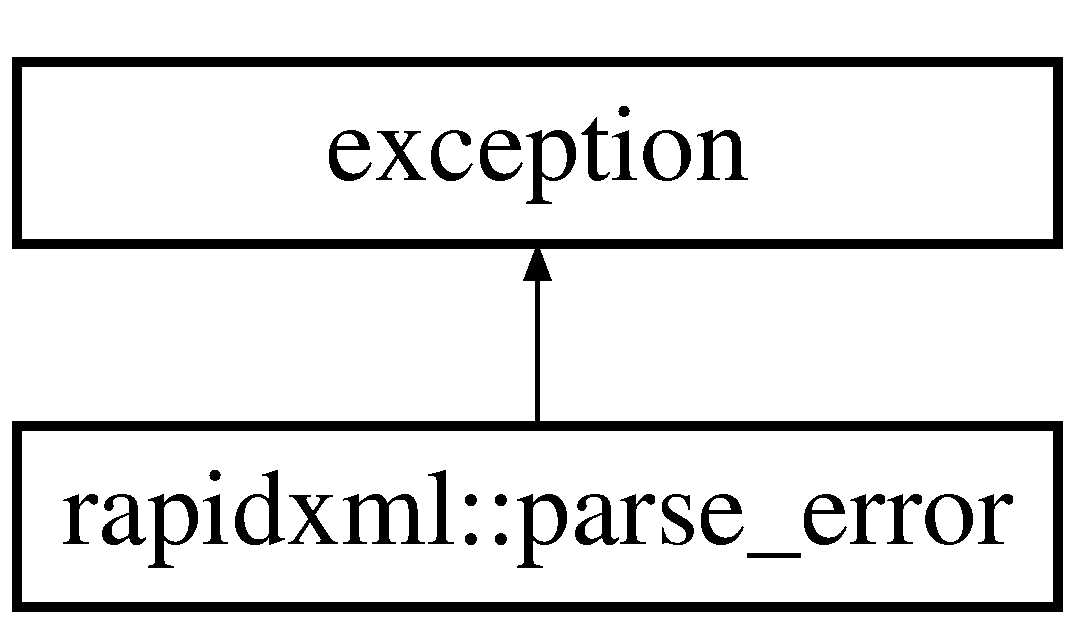
\includegraphics[height=2.000000cm]{classrapidxml_1_1parse__error}
\end{center}
\end{figure}
\subsection*{Public Member Functions}
\begin{DoxyCompactItemize}
\item 
\hyperlink{classrapidxml_1_1parse__error_aea12a301271c393fb627b368fb9f35c1}{parse\+\_\+error} (const char $\ast$\hyperlink{classrapidxml_1_1parse__error_a7665c88639e7466ee1de388a4f85e6fe}{what}, void $\ast$\hyperlink{classrapidxml_1_1parse__error_a3a0ab9e586c1d2b437c340f6622fbec6}{where})
\begin{DoxyCompactList}\small\item\em Constructs parse error. \end{DoxyCompactList}\item 
virtual const char $\ast$ \hyperlink{classrapidxml_1_1parse__error_a7665c88639e7466ee1de388a4f85e6fe}{what} () const   throw ()
\item 
{\footnotesize template$<$class Ch $>$ }\\Ch $\ast$ \hyperlink{classrapidxml_1_1parse__error_a3a0ab9e586c1d2b437c340f6622fbec6}{where} () const 
\end{DoxyCompactItemize}


\subsection{Detailed Description}
Parse error exception. 

This exception is thrown by the parser when an error occurs. Use \hyperlink{classrapidxml_1_1parse__error_a7665c88639e7466ee1de388a4f85e6fe}{what()} function to get human-\/readable error message. Use \hyperlink{classrapidxml_1_1parse__error_a3a0ab9e586c1d2b437c340f6622fbec6}{where()} function to get a pointer to position within source text where error was detected. ~\newline
~\newline
 If throwing exceptions by the parser is undesirable, it can be disabled by defining R\+A\+P\+I\+D\+X\+M\+L\+\_\+\+N\+O\+\_\+\+E\+X\+C\+E\+P\+T\+I\+O\+N\+S macro before \hyperlink{rapidxml_8hpp}{rapidxml.\+hpp} is included. This will cause the parser to call rapidxml\+::parse\+\_\+error\+\_\+handler() function instead of throwing an exception. This function must be defined by the user. ~\newline
~\newline
 This class derives from {\ttfamily std\+::exception} class. 

\subsection{Constructor \& Destructor Documentation}
\hypertarget{classrapidxml_1_1parse__error_aea12a301271c393fb627b368fb9f35c1}{}\index{rapidxml\+::parse\+\_\+error@{rapidxml\+::parse\+\_\+error}!parse\+\_\+error@{parse\+\_\+error}}
\index{parse\+\_\+error@{parse\+\_\+error}!rapidxml\+::parse\+\_\+error@{rapidxml\+::parse\+\_\+error}}
\subsubsection[{parse\+\_\+error(const char $\ast$what, void $\ast$where)}]{\setlength{\rightskip}{0pt plus 5cm}rapidxml\+::parse\+\_\+error\+::parse\+\_\+error (
\begin{DoxyParamCaption}
\item[{const char $\ast$}]{what, }
\item[{void $\ast$}]{where}
\end{DoxyParamCaption}
)\hspace{0.3cm}{\ttfamily [inline]}}\label{classrapidxml_1_1parse__error_aea12a301271c393fb627b368fb9f35c1}


Constructs parse error. 



\subsection{Member Function Documentation}
\hypertarget{classrapidxml_1_1parse__error_a7665c88639e7466ee1de388a4f85e6fe}{}\index{rapidxml\+::parse\+\_\+error@{rapidxml\+::parse\+\_\+error}!what@{what}}
\index{what@{what}!rapidxml\+::parse\+\_\+error@{rapidxml\+::parse\+\_\+error}}
\subsubsection[{what() const }]{\setlength{\rightskip}{0pt plus 5cm}virtual const char$\ast$ rapidxml\+::parse\+\_\+error\+::what (
\begin{DoxyParamCaption}
{}
\end{DoxyParamCaption}
) const throw  ) \hspace{0.3cm}{\ttfamily [inline]}, {\ttfamily [virtual]}}\label{classrapidxml_1_1parse__error_a7665c88639e7466ee1de388a4f85e6fe}
Gets human readable description of error. \begin{DoxyReturn}{Returns}
Pointer to null terminated description of the error. 
\end{DoxyReturn}
\hypertarget{classrapidxml_1_1parse__error_a3a0ab9e586c1d2b437c340f6622fbec6}{}\index{rapidxml\+::parse\+\_\+error@{rapidxml\+::parse\+\_\+error}!where@{where}}
\index{where@{where}!rapidxml\+::parse\+\_\+error@{rapidxml\+::parse\+\_\+error}}
\subsubsection[{where() const }]{\setlength{\rightskip}{0pt plus 5cm}template$<$class Ch $>$ Ch$\ast$ rapidxml\+::parse\+\_\+error\+::where (
\begin{DoxyParamCaption}
{}
\end{DoxyParamCaption}
) const\hspace{0.3cm}{\ttfamily [inline]}}\label{classrapidxml_1_1parse__error_a3a0ab9e586c1d2b437c340f6622fbec6}
Gets pointer to character data where error happened. Ch should be the same as char type of \hyperlink{classrapidxml_1_1xml__document}{xml\+\_\+document} that produced the error. \begin{DoxyReturn}{Returns}
Pointer to location within the parsed string where error occured. 
\end{DoxyReturn}


The documentation for this class was generated from the following file\+:\begin{DoxyCompactItemize}
\item 
/\+Users/brandonmcfarland/\+Desktop/searchdocs/\+Search\+Engine/\+Final\+Project/\hyperlink{rapidxml_8hpp}{rapidxml.\+hpp}\end{DoxyCompactItemize}

\hypertarget{class_query_processor}{}\section{Query\+Processor Class Reference}
\label{class_query_processor}\index{Query\+Processor@{Query\+Processor}}


Holds a relevancy\+Map (unordered\+\_\+map\+\_\+map$<$int, double$>$) that stores the total T\+D/\+I\+D\+F values that a page\+I\+D has for the current query. Keywords A\+N\+D and O\+R will find the intersection and union of potential results, respectively. Control is passed to \hyperlink{class_index_interface}{Index\+Interface} to print the \hyperlink{class_page_info}{Page\+Info} for the best 15 (or less) results.  




{\ttfamily \#include $<$queryprocessor.\+h$>$}

\subsection*{Public Member Functions}
\begin{DoxyCompactItemize}
\item 
\hyperlink{class_query_processor_ac4bebae67b0c08004f26f55957428574}{$\sim$\+Query\+Processor} ()
\item 
\hyperlink{class_query_processor_ac26c0e04d7fd486654a855c7e53027dd}{Query\+Processor} (\hyperlink{class_index_interface}{Index\+Interface} \&the\+Index, bool multi)
\item 
void \hyperlink{class_query_processor_ae54c39816f93865605311fbee9d09d08}{answer\+\_\+query} (istringstream \&query, string full\+\_\+query, bool intersection)
\begin{DoxyCompactList}\small\item\em Start writing to \char`\"{}results\char`\"{}. \end{DoxyCompactList}\item 
void \hyperlink{class_query_processor_ac2e8b45fe91cbcebf9ec32a50e019df6}{display\+\_\+only\+\_\+multi\+\_\+word} (string search\+\_\+string)
\item 
void \hyperlink{class_query_processor_a3e93e0a00cd935ee71497623c8e6d4ad}{display\+\_\+best\+\_\+fifteen\+\_\+results} ()
\begin{DoxyCompactList}\small\item\em Display results in descending order of summed T\+D/\+I\+D\+F value. \end{DoxyCompactList}\item 
void \hyperlink{class_query_processor_ae59525962d93a0087fee0afd689ce1e3}{initiate\+\_\+query} (string query)
\begin{DoxyCompactList}\small\item\em Get input from the user. \end{DoxyCompactList}\item 
void \hyperlink{class_query_processor_ae1f3fdd94b58ac3016ab04873145fec7}{init\+\_\+relev\+\_\+map} (\hyperlink{class_term}{Term} $\ast$term)
\begin{DoxyCompactList}\small\item\em Fill \char`\"{}results\char`\"{} with an initial candidate set. \end{DoxyCompactList}\item 
void \hyperlink{class_query_processor_a29d1767fe229ea175488976673463dcb}{intersection\+\_\+incr\+\_\+relev\+\_\+map} (\hyperlink{class_term}{Term} $\ast$term)
\begin{DoxyCompactList}\small\item\em Explained in \hyperlink{queryprocessor_8cpp}{Query\+Processor.\+cpp}. \end{DoxyCompactList}\item 
void \hyperlink{class_query_processor_aa00880b1308428b29cdc32741f82f4fc}{union\+\_\+incr\+\_\+relev\+\_\+map} (\hyperlink{class_term}{Term} $\ast$term)
\begin{DoxyCompactList}\small\item\em Explained in \hyperlink{queryprocessor_8cpp}{Query\+Processor.\+cpp}. \end{DoxyCompactList}\item 
void \hyperlink{class_query_processor_a75cf5bed3dc75eed5e24aac70535b9d7}{sort\+\_\+results} (bool multi\+\_\+word)
\end{DoxyCompactItemize}


\subsection{Detailed Description}
Holds a relevancy\+Map (unordered\+\_\+map\+\_\+map$<$int, double$>$) that stores the total T\+D/\+I\+D\+F values that a page\+I\+D has for the current query. Keywords A\+N\+D and O\+R will find the intersection and union of potential results, respectively. Control is passed to \hyperlink{class_index_interface}{Index\+Interface} to print the \hyperlink{class_page_info}{Page\+Info} for the best 15 (or less) results. 

\subsection{Constructor \& Destructor Documentation}
\hypertarget{class_query_processor_ac4bebae67b0c08004f26f55957428574}{}\index{Query\+Processor@{Query\+Processor}!````~Query\+Processor@{$\sim$\+Query\+Processor}}
\index{````~Query\+Processor@{$\sim$\+Query\+Processor}!Query\+Processor@{Query\+Processor}}
\subsubsection[{$\sim$\+Query\+Processor()}]{\setlength{\rightskip}{0pt plus 5cm}Query\+Processor\+::$\sim$\+Query\+Processor (
\begin{DoxyParamCaption}
{}
\end{DoxyParamCaption}
)}\label{class_query_processor_ac4bebae67b0c08004f26f55957428574}
\hypertarget{class_query_processor_ac26c0e04d7fd486654a855c7e53027dd}{}\index{Query\+Processor@{Query\+Processor}!Query\+Processor@{Query\+Processor}}
\index{Query\+Processor@{Query\+Processor}!Query\+Processor@{Query\+Processor}}
\subsubsection[{Query\+Processor(\+Index\+Interface \&the\+Index, bool multi)}]{\setlength{\rightskip}{0pt plus 5cm}Query\+Processor\+::\+Query\+Processor (
\begin{DoxyParamCaption}
\item[{{\bf Index\+Interface} \&}]{the\+Index, }
\item[{bool}]{multi}
\end{DoxyParamCaption}
)}\label{class_query_processor_ac26c0e04d7fd486654a855c7e53027dd}


\subsection{Member Function Documentation}
\hypertarget{class_query_processor_ae54c39816f93865605311fbee9d09d08}{}\index{Query\+Processor@{Query\+Processor}!answer\+\_\+query@{answer\+\_\+query}}
\index{answer\+\_\+query@{answer\+\_\+query}!Query\+Processor@{Query\+Processor}}
\subsubsection[{answer\+\_\+query(istringstream \&query, string full\+\_\+query, bool intersection)}]{\setlength{\rightskip}{0pt plus 5cm}void Query\+Processor\+::answer\+\_\+query (
\begin{DoxyParamCaption}
\item[{istringstream \&}]{query, }
\item[{string}]{full\+\_\+query, }
\item[{bool}]{intersection}
\end{DoxyParamCaption}
)}\label{class_query_processor_ae54c39816f93865605311fbee9d09d08}


Start writing to \char`\"{}results\char`\"{}. 

\hypertarget{class_query_processor_a3e93e0a00cd935ee71497623c8e6d4ad}{}\index{Query\+Processor@{Query\+Processor}!display\+\_\+best\+\_\+fifteen\+\_\+results@{display\+\_\+best\+\_\+fifteen\+\_\+results}}
\index{display\+\_\+best\+\_\+fifteen\+\_\+results@{display\+\_\+best\+\_\+fifteen\+\_\+results}!Query\+Processor@{Query\+Processor}}
\subsubsection[{display\+\_\+best\+\_\+fifteen\+\_\+results()}]{\setlength{\rightskip}{0pt plus 5cm}void Query\+Processor\+::display\+\_\+best\+\_\+fifteen\+\_\+results (
\begin{DoxyParamCaption}
{}
\end{DoxyParamCaption}
)}\label{class_query_processor_a3e93e0a00cd935ee71497623c8e6d4ad}


Display results in descending order of summed T\+D/\+I\+D\+F value. 

\hypertarget{class_query_processor_ac2e8b45fe91cbcebf9ec32a50e019df6}{}\index{Query\+Processor@{Query\+Processor}!display\+\_\+only\+\_\+multi\+\_\+word@{display\+\_\+only\+\_\+multi\+\_\+word}}
\index{display\+\_\+only\+\_\+multi\+\_\+word@{display\+\_\+only\+\_\+multi\+\_\+word}!Query\+Processor@{Query\+Processor}}
\subsubsection[{display\+\_\+only\+\_\+multi\+\_\+word(string search\+\_\+string)}]{\setlength{\rightskip}{0pt plus 5cm}void Query\+Processor\+::display\+\_\+only\+\_\+multi\+\_\+word (
\begin{DoxyParamCaption}
\item[{string}]{search\+\_\+string}
\end{DoxyParamCaption}
)}\label{class_query_processor_ac2e8b45fe91cbcebf9ec32a50e019df6}
\hypertarget{class_query_processor_ae1f3fdd94b58ac3016ab04873145fec7}{}\index{Query\+Processor@{Query\+Processor}!init\+\_\+relev\+\_\+map@{init\+\_\+relev\+\_\+map}}
\index{init\+\_\+relev\+\_\+map@{init\+\_\+relev\+\_\+map}!Query\+Processor@{Query\+Processor}}
\subsubsection[{init\+\_\+relev\+\_\+map(\+Term $\ast$term)}]{\setlength{\rightskip}{0pt plus 5cm}void Query\+Processor\+::init\+\_\+relev\+\_\+map (
\begin{DoxyParamCaption}
\item[{{\bf Term} $\ast$}]{term}
\end{DoxyParamCaption}
)}\label{class_query_processor_ae1f3fdd94b58ac3016ab04873145fec7}


Fill \char`\"{}results\char`\"{} with an initial candidate set. 

\hypertarget{class_query_processor_ae59525962d93a0087fee0afd689ce1e3}{}\index{Query\+Processor@{Query\+Processor}!initiate\+\_\+query@{initiate\+\_\+query}}
\index{initiate\+\_\+query@{initiate\+\_\+query}!Query\+Processor@{Query\+Processor}}
\subsubsection[{initiate\+\_\+query(string query)}]{\setlength{\rightskip}{0pt plus 5cm}void Query\+Processor\+::initiate\+\_\+query (
\begin{DoxyParamCaption}
\item[{string}]{query}
\end{DoxyParamCaption}
)}\label{class_query_processor_ae59525962d93a0087fee0afd689ce1e3}


Get input from the user. 

\hypertarget{class_query_processor_a29d1767fe229ea175488976673463dcb}{}\index{Query\+Processor@{Query\+Processor}!intersection\+\_\+incr\+\_\+relev\+\_\+map@{intersection\+\_\+incr\+\_\+relev\+\_\+map}}
\index{intersection\+\_\+incr\+\_\+relev\+\_\+map@{intersection\+\_\+incr\+\_\+relev\+\_\+map}!Query\+Processor@{Query\+Processor}}
\subsubsection[{intersection\+\_\+incr\+\_\+relev\+\_\+map(\+Term $\ast$term)}]{\setlength{\rightskip}{0pt plus 5cm}void Query\+Processor\+::intersection\+\_\+incr\+\_\+relev\+\_\+map (
\begin{DoxyParamCaption}
\item[{{\bf Term} $\ast$}]{term}
\end{DoxyParamCaption}
)}\label{class_query_processor_a29d1767fe229ea175488976673463dcb}


Explained in \hyperlink{queryprocessor_8cpp}{Query\+Processor.\+cpp}. 

\hypertarget{class_query_processor_a75cf5bed3dc75eed5e24aac70535b9d7}{}\index{Query\+Processor@{Query\+Processor}!sort\+\_\+results@{sort\+\_\+results}}
\index{sort\+\_\+results@{sort\+\_\+results}!Query\+Processor@{Query\+Processor}}
\subsubsection[{sort\+\_\+results(bool multi\+\_\+word)}]{\setlength{\rightskip}{0pt plus 5cm}void Query\+Processor\+::sort\+\_\+results (
\begin{DoxyParamCaption}
\item[{bool}]{multi\+\_\+word}
\end{DoxyParamCaption}
)}\label{class_query_processor_a75cf5bed3dc75eed5e24aac70535b9d7}
\hypertarget{class_query_processor_aa00880b1308428b29cdc32741f82f4fc}{}\index{Query\+Processor@{Query\+Processor}!union\+\_\+incr\+\_\+relev\+\_\+map@{union\+\_\+incr\+\_\+relev\+\_\+map}}
\index{union\+\_\+incr\+\_\+relev\+\_\+map@{union\+\_\+incr\+\_\+relev\+\_\+map}!Query\+Processor@{Query\+Processor}}
\subsubsection[{union\+\_\+incr\+\_\+relev\+\_\+map(\+Term $\ast$term)}]{\setlength{\rightskip}{0pt plus 5cm}void Query\+Processor\+::union\+\_\+incr\+\_\+relev\+\_\+map (
\begin{DoxyParamCaption}
\item[{{\bf Term} $\ast$}]{term}
\end{DoxyParamCaption}
)}\label{class_query_processor_aa00880b1308428b29cdc32741f82f4fc}


Explained in \hyperlink{queryprocessor_8cpp}{Query\+Processor.\+cpp}. 



The documentation for this class was generated from the following files\+:\begin{DoxyCompactItemize}
\item 
/\+Users/brandonmcfarland/\+Desktop/searchdocs/\+Search\+Engine/\+Final\+Project/\hyperlink{queryprocessor_8h}{queryprocessor.\+h}\item 
/\+Users/brandonmcfarland/\+Desktop/searchdocs/\+Search\+Engine/\+Final\+Project/\hyperlink{queryprocessor_8cpp}{queryprocessor.\+cpp}\end{DoxyCompactItemize}

\hypertarget{class_term}{}\section{Term Class Reference}
\label{class_term}\index{Term@{Term}}


The heart of the inverted file index. Each \hyperlink{class_term}{Term} object has a name and page\+Map, holding the page\+I\+Ds it\textquotesingle{}s appeared on and the frequency for each page.  




{\ttfamily \#include $<$term.\+h$>$}

\subsection*{Public Member Functions}
\begin{DoxyCompactItemize}
\item 
\hyperlink{class_term_a6943005db5b7e5ca84afcb54a5862d42}{Term} ()
\item 
\hyperlink{class_term_af684aafab11ec6442aed0866b4973afc}{$\sim$\+Term} ()
\item 
\hyperlink{class_term_ae97a04d16b87ac6bebe1057481f962c8}{Term} (string the\+Name, \hyperlink{avltreeinterface_8h_a51573ee2746540a219209715c54ab66c}{page\+Map} \&the\+Aprns)
\begin{DoxyCompactList}\small\item\em The only constructor called. \end{DoxyCompactList}\item 
void \hyperlink{class_term_a2cd7415c99700d9b038517207e1d2738}{init\+\_\+spread\+\_\+and\+\_\+total\+Freq} ()
\begin{DoxyCompactList}\small\item\em The only Terms that will need spread and total\+Freq are result candidates. \end{DoxyCompactList}\item 
void \hyperlink{class_term_a3a48a3273c4bb8755c4623efbf3ebf51}{init\+\_\+tdidfs} (\hyperlink{class_index_interface}{Index\+Interface} \&index)
\begin{DoxyCompactList}\small\item\em Calculate T\+D/\+I\+D\+F values for each document. \end{DoxyCompactList}\item 
void \hyperlink{class_term_a40b76759d6a08c027142527f86d85256}{incrm\+\_\+aprn\+\_\+for\+\_\+page\+I\+D} (int curr\+I\+D)
\begin{DoxyCompactList}\small\item\em Increase a page\+I\+D\textquotesingle{}s frequency by 1. Handles out\+\_\+of\+\_\+range exceptions. \end{DoxyCompactList}\item 
\hyperlink{avltreeinterface_8h_a51573ee2746540a219209715c54ab66c}{page\+Map} \hyperlink{class_term_a3f33daab2cf50371f191c75656aabb66}{get\+\_\+page\+Aprns} ()
\item 
string \hyperlink{class_term_aba11aacf87334a460aae98148699dc46}{get\+\_\+name} ()
\item 
\hyperlink{class_term}{Term} $\ast$ \hyperlink{class_term_a94ed9995429f2c6fd6d0b9556cc61ff7}{get\+\_\+next} ()
\item 
int \hyperlink{class_term_a3b708fc85a3b272d67558600711aca05}{get\+\_\+spread} ()
\item 
int \hyperlink{class_term_a41a8474eb94c1e2e951d23fe164aecd6}{get\+\_\+total\+Freq} ()
\item 
double \hyperlink{class_term_aae2effee196de73962a33d85aeca914c}{get\+\_\+tdidf\+\_\+for\+\_\+page} (int page\+I\+D)
\item 
void \hyperlink{class_term_a2f963514bfacc52e654c94793e25e3d4}{set\+\_\+next} (\hyperlink{class_term}{Term} $\ast$the\+Next)
\item 
void \hyperlink{class_term_ae0e0bd5c7411fa03aeb2c92464dd921b}{write\+\_\+term} (ofstream \&persistence)
\begin{DoxyCompactList}\small\item\em Write \hyperlink{class_term}{Term}\textquotesingle{}s info to the persistence index. \end{DoxyCompactList}\end{DoxyCompactItemize}


\subsection{Detailed Description}
The heart of the inverted file index. Each \hyperlink{class_term}{Term} object has a name and page\+Map, holding the page\+I\+Ds it\textquotesingle{}s appeared on and the frequency for each page. 

\subsection{Constructor \& Destructor Documentation}
\hypertarget{class_term_a6943005db5b7e5ca84afcb54a5862d42}{}\index{Term@{Term}!Term@{Term}}
\index{Term@{Term}!Term@{Term}}
\subsubsection[{Term()}]{\setlength{\rightskip}{0pt plus 5cm}Term\+::\+Term (
\begin{DoxyParamCaption}
{}
\end{DoxyParamCaption}
)}\label{class_term_a6943005db5b7e5ca84afcb54a5862d42}
\hypertarget{class_term_af684aafab11ec6442aed0866b4973afc}{}\index{Term@{Term}!````~Term@{$\sim$\+Term}}
\index{````~Term@{$\sim$\+Term}!Term@{Term}}
\subsubsection[{$\sim$\+Term()}]{\setlength{\rightskip}{0pt plus 5cm}Term\+::$\sim$\+Term (
\begin{DoxyParamCaption}
{}
\end{DoxyParamCaption}
)}\label{class_term_af684aafab11ec6442aed0866b4973afc}
\hypertarget{class_term_ae97a04d16b87ac6bebe1057481f962c8}{}\index{Term@{Term}!Term@{Term}}
\index{Term@{Term}!Term@{Term}}
\subsubsection[{Term(string the\+Name, page\+Map \&the\+Aprns)}]{\setlength{\rightskip}{0pt plus 5cm}Term\+::\+Term (
\begin{DoxyParamCaption}
\item[{string}]{the\+Name, }
\item[{{\bf page\+Map} \&}]{the\+Aprns}
\end{DoxyParamCaption}
)}\label{class_term_ae97a04d16b87ac6bebe1057481f962c8}


The only constructor called. 



\subsection{Member Function Documentation}
\hypertarget{class_term_aba11aacf87334a460aae98148699dc46}{}\index{Term@{Term}!get\+\_\+name@{get\+\_\+name}}
\index{get\+\_\+name@{get\+\_\+name}!Term@{Term}}
\subsubsection[{get\+\_\+name()}]{\setlength{\rightskip}{0pt plus 5cm}string Term\+::get\+\_\+name (
\begin{DoxyParamCaption}
{}
\end{DoxyParamCaption}
)}\label{class_term_aba11aacf87334a460aae98148699dc46}
\hypertarget{class_term_a94ed9995429f2c6fd6d0b9556cc61ff7}{}\index{Term@{Term}!get\+\_\+next@{get\+\_\+next}}
\index{get\+\_\+next@{get\+\_\+next}!Term@{Term}}
\subsubsection[{get\+\_\+next()}]{\setlength{\rightskip}{0pt plus 5cm}{\bf Term} $\ast$ Term\+::get\+\_\+next (
\begin{DoxyParamCaption}
{}
\end{DoxyParamCaption}
)}\label{class_term_a94ed9995429f2c6fd6d0b9556cc61ff7}
\hypertarget{class_term_a3f33daab2cf50371f191c75656aabb66}{}\index{Term@{Term}!get\+\_\+page\+Aprns@{get\+\_\+page\+Aprns}}
\index{get\+\_\+page\+Aprns@{get\+\_\+page\+Aprns}!Term@{Term}}
\subsubsection[{get\+\_\+page\+Aprns()}]{\setlength{\rightskip}{0pt plus 5cm}{\bf page\+Map} Term\+::get\+\_\+page\+Aprns (
\begin{DoxyParamCaption}
{}
\end{DoxyParamCaption}
)}\label{class_term_a3f33daab2cf50371f191c75656aabb66}
\hypertarget{class_term_a3b708fc85a3b272d67558600711aca05}{}\index{Term@{Term}!get\+\_\+spread@{get\+\_\+spread}}
\index{get\+\_\+spread@{get\+\_\+spread}!Term@{Term}}
\subsubsection[{get\+\_\+spread()}]{\setlength{\rightskip}{0pt plus 5cm}int Term\+::get\+\_\+spread (
\begin{DoxyParamCaption}
{}
\end{DoxyParamCaption}
)}\label{class_term_a3b708fc85a3b272d67558600711aca05}
\hypertarget{class_term_aae2effee196de73962a33d85aeca914c}{}\index{Term@{Term}!get\+\_\+tdidf\+\_\+for\+\_\+page@{get\+\_\+tdidf\+\_\+for\+\_\+page}}
\index{get\+\_\+tdidf\+\_\+for\+\_\+page@{get\+\_\+tdidf\+\_\+for\+\_\+page}!Term@{Term}}
\subsubsection[{get\+\_\+tdidf\+\_\+for\+\_\+page(int page\+I\+D)}]{\setlength{\rightskip}{0pt plus 5cm}double Term\+::get\+\_\+tdidf\+\_\+for\+\_\+page (
\begin{DoxyParamCaption}
\item[{int}]{page\+I\+D}
\end{DoxyParamCaption}
)}\label{class_term_aae2effee196de73962a33d85aeca914c}
\hypertarget{class_term_a41a8474eb94c1e2e951d23fe164aecd6}{}\index{Term@{Term}!get\+\_\+total\+Freq@{get\+\_\+total\+Freq}}
\index{get\+\_\+total\+Freq@{get\+\_\+total\+Freq}!Term@{Term}}
\subsubsection[{get\+\_\+total\+Freq()}]{\setlength{\rightskip}{0pt plus 5cm}int Term\+::get\+\_\+total\+Freq (
\begin{DoxyParamCaption}
{}
\end{DoxyParamCaption}
)}\label{class_term_a41a8474eb94c1e2e951d23fe164aecd6}
\hypertarget{class_term_a40b76759d6a08c027142527f86d85256}{}\index{Term@{Term}!incrm\+\_\+aprn\+\_\+for\+\_\+page\+I\+D@{incrm\+\_\+aprn\+\_\+for\+\_\+page\+I\+D}}
\index{incrm\+\_\+aprn\+\_\+for\+\_\+page\+I\+D@{incrm\+\_\+aprn\+\_\+for\+\_\+page\+I\+D}!Term@{Term}}
\subsubsection[{incrm\+\_\+aprn\+\_\+for\+\_\+page\+I\+D(int curr\+I\+D)}]{\setlength{\rightskip}{0pt plus 5cm}void Term\+::incrm\+\_\+aprn\+\_\+for\+\_\+page\+I\+D (
\begin{DoxyParamCaption}
\item[{int}]{curr\+I\+D}
\end{DoxyParamCaption}
)}\label{class_term_a40b76759d6a08c027142527f86d85256}


Increase a page\+I\+D\textquotesingle{}s frequency by 1. Handles out\+\_\+of\+\_\+range exceptions. 

\hypertarget{class_term_a2cd7415c99700d9b038517207e1d2738}{}\index{Term@{Term}!init\+\_\+spread\+\_\+and\+\_\+total\+Freq@{init\+\_\+spread\+\_\+and\+\_\+total\+Freq}}
\index{init\+\_\+spread\+\_\+and\+\_\+total\+Freq@{init\+\_\+spread\+\_\+and\+\_\+total\+Freq}!Term@{Term}}
\subsubsection[{init\+\_\+spread\+\_\+and\+\_\+total\+Freq()}]{\setlength{\rightskip}{0pt plus 5cm}void Term\+::init\+\_\+spread\+\_\+and\+\_\+total\+Freq (
\begin{DoxyParamCaption}
{}
\end{DoxyParamCaption}
)}\label{class_term_a2cd7415c99700d9b038517207e1d2738}


The only Terms that will need spread and total\+Freq are result candidates. 

\hypertarget{class_term_a3a48a3273c4bb8755c4623efbf3ebf51}{}\index{Term@{Term}!init\+\_\+tdidfs@{init\+\_\+tdidfs}}
\index{init\+\_\+tdidfs@{init\+\_\+tdidfs}!Term@{Term}}
\subsubsection[{init\+\_\+tdidfs(\+Index\+Interface \&index)}]{\setlength{\rightskip}{0pt plus 5cm}void Term\+::init\+\_\+tdidfs (
\begin{DoxyParamCaption}
\item[{{\bf Index\+Interface} \&}]{index}
\end{DoxyParamCaption}
)}\label{class_term_a3a48a3273c4bb8755c4623efbf3ebf51}


Calculate T\+D/\+I\+D\+F values for each document. 

\hypertarget{class_term_a2f963514bfacc52e654c94793e25e3d4}{}\index{Term@{Term}!set\+\_\+next@{set\+\_\+next}}
\index{set\+\_\+next@{set\+\_\+next}!Term@{Term}}
\subsubsection[{set\+\_\+next(\+Term $\ast$the\+Next)}]{\setlength{\rightskip}{0pt plus 5cm}void Term\+::set\+\_\+next (
\begin{DoxyParamCaption}
\item[{{\bf Term} $\ast$}]{the\+Next}
\end{DoxyParamCaption}
)}\label{class_term_a2f963514bfacc52e654c94793e25e3d4}
\hypertarget{class_term_ae0e0bd5c7411fa03aeb2c92464dd921b}{}\index{Term@{Term}!write\+\_\+term@{write\+\_\+term}}
\index{write\+\_\+term@{write\+\_\+term}!Term@{Term}}
\subsubsection[{write\+\_\+term(ofstream \&persistence)}]{\setlength{\rightskip}{0pt plus 5cm}void Term\+::write\+\_\+term (
\begin{DoxyParamCaption}
\item[{ofstream \&}]{persistence}
\end{DoxyParamCaption}
)}\label{class_term_ae0e0bd5c7411fa03aeb2c92464dd921b}


Write \hyperlink{class_term}{Term}\textquotesingle{}s info to the persistence index. 



The documentation for this class was generated from the following files\+:\begin{DoxyCompactItemize}
\item 
/\+Users/brandonmcfarland/\+Desktop/searchdocs/\+Search\+Engine/\+Final\+Project/\hyperlink{term_8h}{term.\+h}\item 
/\+Users/brandonmcfarland/\+Desktop/searchdocs/\+Search\+Engine/\+Final\+Project/\hyperlink{term_8cpp}{term.\+cpp}\end{DoxyCompactItemize}

\hypertarget{class_term_bucket}{}\section{Term\+Bucket Class Reference}
\label{class_term_bucket}\index{Term\+Bucket@{Term\+Bucket}}


A linked list of Term$\ast$s (b/c \hyperlink{class_hash_table_index}{Hash\+Table\+Index} handles collisions by chanining).  




{\ttfamily \#include $<$termbucket.\+h$>$}

\subsection*{Public Member Functions}
\begin{DoxyCompactItemize}
\item 
\hyperlink{class_term_bucket_a2f45be1b657541ccf0d255b5a4a4b6e7}{Term\+Bucket} ()
\item 
\hyperlink{class_term_bucket_a2995af64e66038cce2604cd26f27b743}{$\sim$\+Term\+Bucket} ()
\item 
void \hyperlink{class_term_bucket_ad8bccbf5570ca903ec3b5b7e6d90da83}{add\+\_\+term\+\_\+to\+\_\+bucket} (\hyperlink{class_term}{Term} $\ast$term)
\begin{DoxyCompactList}\small\item\em Append Term$\ast$ to linked list. \end{DoxyCompactList}\item 
\hyperlink{class_term}{Term} $\ast$ \hyperlink{class_term_bucket_a637756154b34dce701969c0e930a0de5}{find} (string term)
\begin{DoxyCompactList}\small\item\em Search the bucket for the Term$\ast$ corresponding with a provided name. If it doesn\textquotesingle{}t exist, retrun N\+U\+L\+L. \end{DoxyCompactList}\item 
bool \hyperlink{class_term_bucket_aa5f0d336448063bea5d33a090ac09785}{has\+\_\+word} (string term)
\item 
void \hyperlink{class_term_bucket_a9f861191a65c27611a4b15773b379716}{write\+\_\+term\+\_\+bucket} (ofstream \&persistence)
\begin{DoxyCompactList}\small\item\em For each \hyperlink{class_term}{Term} in the bucket, call write\+\_\+term. \end{DoxyCompactList}\item 
void \hyperlink{class_term_bucket_a8aa95625bf111166efd958f34e0da1e2}{clear} ()
\end{DoxyCompactItemize}


\subsection{Detailed Description}
A linked list of Term$\ast$s (b/c \hyperlink{class_hash_table_index}{Hash\+Table\+Index} handles collisions by chanining). 

\subsection{Constructor \& Destructor Documentation}
\hypertarget{class_term_bucket_a2f45be1b657541ccf0d255b5a4a4b6e7}{}\index{Term\+Bucket@{Term\+Bucket}!Term\+Bucket@{Term\+Bucket}}
\index{Term\+Bucket@{Term\+Bucket}!Term\+Bucket@{Term\+Bucket}}
\subsubsection[{Term\+Bucket()}]{\setlength{\rightskip}{0pt plus 5cm}Term\+Bucket\+::\+Term\+Bucket (
\begin{DoxyParamCaption}
{}
\end{DoxyParamCaption}
)}\label{class_term_bucket_a2f45be1b657541ccf0d255b5a4a4b6e7}
\hypertarget{class_term_bucket_a2995af64e66038cce2604cd26f27b743}{}\index{Term\+Bucket@{Term\+Bucket}!````~Term\+Bucket@{$\sim$\+Term\+Bucket}}
\index{````~Term\+Bucket@{$\sim$\+Term\+Bucket}!Term\+Bucket@{Term\+Bucket}}
\subsubsection[{$\sim$\+Term\+Bucket()}]{\setlength{\rightskip}{0pt plus 5cm}Term\+Bucket\+::$\sim$\+Term\+Bucket (
\begin{DoxyParamCaption}
{}
\end{DoxyParamCaption}
)}\label{class_term_bucket_a2995af64e66038cce2604cd26f27b743}


\subsection{Member Function Documentation}
\hypertarget{class_term_bucket_ad8bccbf5570ca903ec3b5b7e6d90da83}{}\index{Term\+Bucket@{Term\+Bucket}!add\+\_\+term\+\_\+to\+\_\+bucket@{add\+\_\+term\+\_\+to\+\_\+bucket}}
\index{add\+\_\+term\+\_\+to\+\_\+bucket@{add\+\_\+term\+\_\+to\+\_\+bucket}!Term\+Bucket@{Term\+Bucket}}
\subsubsection[{add\+\_\+term\+\_\+to\+\_\+bucket(\+Term $\ast$term)}]{\setlength{\rightskip}{0pt plus 5cm}void Term\+Bucket\+::add\+\_\+term\+\_\+to\+\_\+bucket (
\begin{DoxyParamCaption}
\item[{{\bf Term} $\ast$}]{term}
\end{DoxyParamCaption}
)}\label{class_term_bucket_ad8bccbf5570ca903ec3b5b7e6d90da83}


Append Term$\ast$ to linked list. 

\hypertarget{class_term_bucket_a8aa95625bf111166efd958f34e0da1e2}{}\index{Term\+Bucket@{Term\+Bucket}!clear@{clear}}
\index{clear@{clear}!Term\+Bucket@{Term\+Bucket}}
\subsubsection[{clear()}]{\setlength{\rightskip}{0pt plus 5cm}void Term\+Bucket\+::clear (
\begin{DoxyParamCaption}
{}
\end{DoxyParamCaption}
)}\label{class_term_bucket_a8aa95625bf111166efd958f34e0da1e2}
\hypertarget{class_term_bucket_a637756154b34dce701969c0e930a0de5}{}\index{Term\+Bucket@{Term\+Bucket}!find@{find}}
\index{find@{find}!Term\+Bucket@{Term\+Bucket}}
\subsubsection[{find(string term)}]{\setlength{\rightskip}{0pt plus 5cm}{\bf Term} $\ast$ Term\+Bucket\+::find (
\begin{DoxyParamCaption}
\item[{string}]{term}
\end{DoxyParamCaption}
)}\label{class_term_bucket_a637756154b34dce701969c0e930a0de5}


Search the bucket for the Term$\ast$ corresponding with a provided name. If it doesn\textquotesingle{}t exist, retrun N\+U\+L\+L. 

\hypertarget{class_term_bucket_aa5f0d336448063bea5d33a090ac09785}{}\index{Term\+Bucket@{Term\+Bucket}!has\+\_\+word@{has\+\_\+word}}
\index{has\+\_\+word@{has\+\_\+word}!Term\+Bucket@{Term\+Bucket}}
\subsubsection[{has\+\_\+word(string term)}]{\setlength{\rightskip}{0pt plus 5cm}bool Term\+Bucket\+::has\+\_\+word (
\begin{DoxyParamCaption}
\item[{string}]{term}
\end{DoxyParamCaption}
)}\label{class_term_bucket_aa5f0d336448063bea5d33a090ac09785}
\hypertarget{class_term_bucket_a9f861191a65c27611a4b15773b379716}{}\index{Term\+Bucket@{Term\+Bucket}!write\+\_\+term\+\_\+bucket@{write\+\_\+term\+\_\+bucket}}
\index{write\+\_\+term\+\_\+bucket@{write\+\_\+term\+\_\+bucket}!Term\+Bucket@{Term\+Bucket}}
\subsubsection[{write\+\_\+term\+\_\+bucket(ofstream \&persistence)}]{\setlength{\rightskip}{0pt plus 5cm}void Term\+Bucket\+::write\+\_\+term\+\_\+bucket (
\begin{DoxyParamCaption}
\item[{ofstream \&}]{persistence}
\end{DoxyParamCaption}
)}\label{class_term_bucket_a9f861191a65c27611a4b15773b379716}


For each \hyperlink{class_term}{Term} in the bucket, call write\+\_\+term. 



The documentation for this class was generated from the following files\+:\begin{DoxyCompactItemize}
\item 
/\+Users/brandonmcfarland/\+Desktop/searchdocs/\+Search\+Engine/\+Final\+Project/\hyperlink{termbucket_8h}{termbucket.\+h}\item 
/\+Users/brandonmcfarland/\+Desktop/searchdocs/\+Search\+Engine/\+Final\+Project/\hyperlink{termbucket_8cpp}{termbucket.\+cpp}\end{DoxyCompactItemize}

\hypertarget{class_timer}{}\section{Timer Class Reference}
\label{class_timer}\index{Timer@{Timer}}


checks for the function time of each function when called  




{\ttfamily \#include $<$timer.\+h$>$}

\subsection*{Public Member Functions}
\begin{DoxyCompactItemize}
\item 
\hyperlink{class_timer_a5f16e8da27d2a5a5242dead46de05d97}{Timer} ()
\begin{DoxyCompactList}\small\item\em constructor \end{DoxyCompactList}\item 
\hyperlink{class_timer_a0faa0537ddf1918baa13d64cc64fe1e9}{Timer} (string the\+Name)
\begin{DoxyCompactList}\small\item\em overloaded constructor \end{DoxyCompactList}\item 
\hyperlink{class_timer_a14fa469c4c295c5fa6e66a4ad1092146}{$\sim$\+Timer} ()
\begin{DoxyCompactList}\small\item\em destructor \end{DoxyCompactList}\end{DoxyCompactItemize}


\subsection{Detailed Description}
checks for the function time of each function when called 

\subsection{Constructor \& Destructor Documentation}
\hypertarget{class_timer_a5f16e8da27d2a5a5242dead46de05d97}{}\index{Timer@{Timer}!Timer@{Timer}}
\index{Timer@{Timer}!Timer@{Timer}}
\subsubsection[{Timer()}]{\setlength{\rightskip}{0pt plus 5cm}Timer\+::\+Timer (
\begin{DoxyParamCaption}
{}
\end{DoxyParamCaption}
)}\label{class_timer_a5f16e8da27d2a5a5242dead46de05d97}


constructor 

\hypertarget{class_timer_a0faa0537ddf1918baa13d64cc64fe1e9}{}\index{Timer@{Timer}!Timer@{Timer}}
\index{Timer@{Timer}!Timer@{Timer}}
\subsubsection[{Timer(string the\+Name)}]{\setlength{\rightskip}{0pt plus 5cm}Timer\+::\+Timer (
\begin{DoxyParamCaption}
\item[{string}]{the\+Name}
\end{DoxyParamCaption}
)}\label{class_timer_a0faa0537ddf1918baa13d64cc64fe1e9}


overloaded constructor 

\hypertarget{class_timer_a14fa469c4c295c5fa6e66a4ad1092146}{}\index{Timer@{Timer}!````~Timer@{$\sim$\+Timer}}
\index{````~Timer@{$\sim$\+Timer}!Timer@{Timer}}
\subsubsection[{$\sim$\+Timer()}]{\setlength{\rightskip}{0pt plus 5cm}Timer\+::$\sim$\+Timer (
\begin{DoxyParamCaption}
{}
\end{DoxyParamCaption}
)}\label{class_timer_a14fa469c4c295c5fa6e66a4ad1092146}


destructor 



The documentation for this class was generated from the following files\+:\begin{DoxyCompactItemize}
\item 
/\+Users/brandonmcfarland/\+Desktop/searchdocs/\+Search\+Engine/\+Final\+Project/\hyperlink{timer_8h}{timer.\+h}\item 
/\+Users/brandonmcfarland/\+Desktop/searchdocs/\+Search\+Engine/\+Final\+Project/\hyperlink{timer_8cpp}{timer.\+cpp}\end{DoxyCompactItemize}

\hypertarget{classunordered__multimap}{}\section{unordered\+\_\+multimap$<$ \+\_\+\+Key, \+\_\+\+Tp, \+\_\+\+Hash, \+\_\+\+Pred, \+\_\+\+Alloc $>$ Class Template Reference}
\label{classunordered__multimap}\index{unordered\+\_\+multimap$<$ \+\_\+\+Key, \+\_\+\+Tp, \+\_\+\+Hash, \+\_\+\+Pred, \+\_\+\+Alloc $>$@{unordered\+\_\+multimap$<$ \+\_\+\+Key, \+\_\+\+Tp, \+\_\+\+Hash, \+\_\+\+Pred, \+\_\+\+Alloc $>$}}


{\ttfamily \#include $<$mapping.\+h$>$}

\subsection*{Public Types}
\begin{DoxyCompactItemize}
\item 
typedef \+\_\+\+Key \hyperlink{classunordered__multimap_a2902747087a03531493d30e9840f67d9}{key\+\_\+type}
\item 
typedef \+\_\+\+Tp \hyperlink{classunordered__multimap_a50bc9bc504d96ff3c7ca7db1f428eb5e}{mapped\+\_\+type}
\item 
typedef \+\_\+\+Hash \hyperlink{classunordered__multimap_a93affc33f5ee930cff353ff62d20daef}{hasher}
\item 
typedef \+\_\+\+Pred \hyperlink{classunordered__multimap_aeed817e3baaf0771b8336eb2477f4f02}{key\+\_\+equal}
\item 
typedef \+\_\+\+Alloc \hyperlink{classunordered__multimap_a821ff3be687cecd9ef325efa93759c19}{allocator\+\_\+type}
\item 
typedef pair$<$ const \hyperlink{classunordered__multimap_a2902747087a03531493d30e9840f67d9}{key\+\_\+type}, \hyperlink{classunordered__multimap_a50bc9bc504d96ff3c7ca7db1f428eb5e}{mapped\+\_\+type} $>$ \hyperlink{classunordered__multimap_a106d390dc0deafc47f10d3943b247ee6}{value\+\_\+type}
\item 
typedef pair$<$ \hyperlink{classunordered__multimap_a2902747087a03531493d30e9840f67d9}{key\+\_\+type}, \hyperlink{classunordered__multimap_a50bc9bc504d96ff3c7ca7db1f428eb5e}{mapped\+\_\+type} $>$ \hyperlink{classunordered__multimap_a02f7a45f9e19d7a13e361aa3509af744}{\+\_\+\+\_\+nc\+\_\+value\+\_\+type}
\item 
typedef \hyperlink{classunordered__multimap_a106d390dc0deafc47f10d3943b247ee6}{value\+\_\+type} \& \hyperlink{classunordered__multimap_a0c14a599081fd7cef3adfd73572a78be}{reference}
\item 
typedef const \hyperlink{classunordered__multimap_a106d390dc0deafc47f10d3943b247ee6}{value\+\_\+type} \& \hyperlink{classunordered__multimap_ab3aedd41dcc9c645d596c98ba3379826}{const\+\_\+reference}
\item 
typedef \+\_\+\+\_\+alloc\+\_\+traits\+::pointer \hyperlink{classunordered__multimap_ace9882ddb645e0c73785f46e8c0fc9f4}{pointer}
\item 
typedef \+\_\+\+\_\+alloc\+\_\+traits\+::const\+\_\+pointer \hyperlink{classunordered__multimap_ac431051a949a339b15eb3c6f0ff5dccf}{const\+\_\+pointer}
\item 
typedef \+\_\+\+\_\+alloc\+\_\+traits\+::size\+\_\+type \hyperlink{classunordered__multimap_a977c4093df6d4d0302f280de19af4b58}{size\+\_\+type}
\item 
typedef \+\_\+\+\_\+alloc\+\_\+traits\+::difference\+\_\+type \hyperlink{classunordered__multimap_ae01816b9f8883bc381dee433486054de}{difference\+\_\+type}
\item 
typedef \hyperlink{class____hash__map__iterator}{\+\_\+\+\_\+hash\+\_\+map\+\_\+iterator}$<$ typename \+\_\+\+\_\+table\+::iterator $>$ \hyperlink{classunordered__multimap_a7b508cae41ac3a258ca80609ec43db47}{iterator}
\item 
typedef \hyperlink{class____hash__map__const__iterator}{\+\_\+\+\_\+hash\+\_\+map\+\_\+const\+\_\+iterator}$<$ typename \+\_\+\+\_\+table\+::const\+\_\+iterator $>$ \hyperlink{classunordered__multimap_a3cb373bd19680f9933781c04905fde39}{const\+\_\+iterator}
\item 
typedef \hyperlink{class____hash__map__iterator}{\+\_\+\+\_\+hash\+\_\+map\+\_\+iterator}$<$ typename \+\_\+\+\_\+table\+::local\+\_\+iterator $>$ \hyperlink{classunordered__multimap_a672fd63d94f807d130e2026d2863d40c}{local\+\_\+iterator}
\item 
typedef \hyperlink{class____hash__map__const__iterator}{\+\_\+\+\_\+hash\+\_\+map\+\_\+const\+\_\+iterator}$<$ typename \+\_\+\+\_\+table\+::const\+\_\+local\+\_\+iterator $>$ \hyperlink{classunordered__multimap_a4813834c894681f449b5afe718336482}{const\+\_\+local\+\_\+iterator}
\item 
typedef \+\_\+\+Key \hyperlink{classunordered__multimap_a2902747087a03531493d30e9840f67d9}{key\+\_\+type}
\item 
typedef \+\_\+\+Tp \hyperlink{classunordered__multimap_a50bc9bc504d96ff3c7ca7db1f428eb5e}{mapped\+\_\+type}
\item 
typedef \+\_\+\+Hash \hyperlink{classunordered__multimap_a93affc33f5ee930cff353ff62d20daef}{hasher}
\item 
typedef \+\_\+\+Pred \hyperlink{classunordered__multimap_aeed817e3baaf0771b8336eb2477f4f02}{key\+\_\+equal}
\item 
typedef \+\_\+\+Alloc \hyperlink{classunordered__multimap_a821ff3be687cecd9ef325efa93759c19}{allocator\+\_\+type}
\item 
typedef pair$<$ const \hyperlink{classunordered__multimap_a2902747087a03531493d30e9840f67d9}{key\+\_\+type}, \hyperlink{classunordered__multimap_a50bc9bc504d96ff3c7ca7db1f428eb5e}{mapped\+\_\+type} $>$ \hyperlink{classunordered__multimap_a106d390dc0deafc47f10d3943b247ee6}{value\+\_\+type}
\item 
typedef pair$<$ \hyperlink{classunordered__multimap_a2902747087a03531493d30e9840f67d9}{key\+\_\+type}, \hyperlink{classunordered__multimap_a50bc9bc504d96ff3c7ca7db1f428eb5e}{mapped\+\_\+type} $>$ \hyperlink{classunordered__multimap_a02f7a45f9e19d7a13e361aa3509af744}{\+\_\+\+\_\+nc\+\_\+value\+\_\+type}
\item 
typedef \hyperlink{classunordered__multimap_a106d390dc0deafc47f10d3943b247ee6}{value\+\_\+type} \& \hyperlink{classunordered__multimap_a0c14a599081fd7cef3adfd73572a78be}{reference}
\item 
typedef const \hyperlink{classunordered__multimap_a106d390dc0deafc47f10d3943b247ee6}{value\+\_\+type} \& \hyperlink{classunordered__multimap_ab3aedd41dcc9c645d596c98ba3379826}{const\+\_\+reference}
\item 
typedef \+\_\+\+\_\+alloc\+\_\+traits\+::pointer \hyperlink{classunordered__multimap_ace9882ddb645e0c73785f46e8c0fc9f4}{pointer}
\item 
typedef \+\_\+\+\_\+alloc\+\_\+traits\+::const\+\_\+pointer \hyperlink{classunordered__multimap_ac431051a949a339b15eb3c6f0ff5dccf}{const\+\_\+pointer}
\item 
typedef \+\_\+\+\_\+alloc\+\_\+traits\+::size\+\_\+type \hyperlink{classunordered__multimap_a977c4093df6d4d0302f280de19af4b58}{size\+\_\+type}
\item 
typedef \+\_\+\+\_\+alloc\+\_\+traits\+::difference\+\_\+type \hyperlink{classunordered__multimap_ae01816b9f8883bc381dee433486054de}{difference\+\_\+type}
\item 
typedef \hyperlink{class____hash__map__iterator}{\+\_\+\+\_\+hash\+\_\+map\+\_\+iterator}$<$ typename \+\_\+\+\_\+table\+::iterator $>$ \hyperlink{classunordered__multimap_a7b508cae41ac3a258ca80609ec43db47}{iterator}
\item 
typedef \hyperlink{class____hash__map__const__iterator}{\+\_\+\+\_\+hash\+\_\+map\+\_\+const\+\_\+iterator}$<$ typename \+\_\+\+\_\+table\+::const\+\_\+iterator $>$ \hyperlink{classunordered__multimap_a3cb373bd19680f9933781c04905fde39}{const\+\_\+iterator}
\item 
typedef \hyperlink{class____hash__map__iterator}{\+\_\+\+\_\+hash\+\_\+map\+\_\+iterator}$<$ typename \+\_\+\+\_\+table\+::local\+\_\+iterator $>$ \hyperlink{classunordered__multimap_a672fd63d94f807d130e2026d2863d40c}{local\+\_\+iterator}
\item 
typedef \hyperlink{class____hash__map__const__iterator}{\+\_\+\+\_\+hash\+\_\+map\+\_\+const\+\_\+iterator}$<$ typename \+\_\+\+\_\+table\+::const\+\_\+local\+\_\+iterator $>$ \hyperlink{classunordered__multimap_a4813834c894681f449b5afe718336482}{const\+\_\+local\+\_\+iterator}
\end{DoxyCompactItemize}
\subsection*{Public Member Functions}
\begin{DoxyCompactItemize}
\item 
\+\_\+\+L\+I\+B\+C\+P\+P\+\_\+\+I\+N\+L\+I\+N\+E\+\_\+\+V\+I\+S\+I\+B\+I\+L\+I\+T\+Y \hyperlink{classunordered__multimap_aa1f6b416690d0460698d001b15bede02}{unordered\+\_\+multimap} () \+\_\+\+N\+O\+E\+X\+C\+E\+P\+T\+\_\+(is\+\_\+nothrow\+\_\+default\+\_\+constructible$<$ \+\_\+\+\_\+table $>$
\item 
\hyperlink{classunordered__multimap_ad5a1781d30c2d18ba126f2efa19671f1}{unordered\+\_\+multimap} (\hyperlink{classunordered__multimap_a977c4093df6d4d0302f280de19af4b58}{size\+\_\+type} \+\_\+\+\_\+n, const \hyperlink{classunordered__multimap_a93affc33f5ee930cff353ff62d20daef}{hasher} \&\+\_\+\+\_\+hf=\hyperlink{classunordered__multimap_a93affc33f5ee930cff353ff62d20daef}{hasher}(), const \hyperlink{classunordered__multimap_aeed817e3baaf0771b8336eb2477f4f02}{key\+\_\+equal} \&\+\_\+\+\_\+eql=\hyperlink{classunordered__multimap_aeed817e3baaf0771b8336eb2477f4f02}{key\+\_\+equal}())
\item 
\hyperlink{classunordered__multimap_a4df1734040516b3fa505d5ad08404555}{unordered\+\_\+multimap} (\hyperlink{classunordered__multimap_a977c4093df6d4d0302f280de19af4b58}{size\+\_\+type} \+\_\+\+\_\+n, const \hyperlink{classunordered__multimap_a93affc33f5ee930cff353ff62d20daef}{hasher} \&\+\_\+\+\_\+hf, const \hyperlink{classunordered__multimap_aeed817e3baaf0771b8336eb2477f4f02}{key\+\_\+equal} \&\+\_\+\+\_\+eql, const \hyperlink{classunordered__multimap_a821ff3be687cecd9ef325efa93759c19}{allocator\+\_\+type} \&\+\_\+\+\_\+a)
\item 
{\footnotesize template$<$class \+\_\+\+Input\+Iterator $>$ }\\\hyperlink{classunordered__multimap_af7829207aef36c7dd52a7e55780ed86d}{unordered\+\_\+multimap} (\+\_\+\+Input\+Iterator \+\_\+\+\_\+first, \+\_\+\+Input\+Iterator \+\_\+\+\_\+last)
\item 
{\footnotesize template$<$class \+\_\+\+Input\+Iterator $>$ }\\\hyperlink{classunordered__multimap_af00ca614f7641ef62c552540dd846d46}{unordered\+\_\+multimap} (\+\_\+\+Input\+Iterator \+\_\+\+\_\+first, \+\_\+\+Input\+Iterator \+\_\+\+\_\+last, \hyperlink{classunordered__multimap_a977c4093df6d4d0302f280de19af4b58}{size\+\_\+type} \+\_\+\+\_\+n, const \hyperlink{classunordered__multimap_a93affc33f5ee930cff353ff62d20daef}{hasher} \&\+\_\+\+\_\+hf=\hyperlink{classunordered__multimap_a93affc33f5ee930cff353ff62d20daef}{hasher}(), const \hyperlink{classunordered__multimap_aeed817e3baaf0771b8336eb2477f4f02}{key\+\_\+equal} \&\+\_\+\+\_\+eql=\hyperlink{classunordered__multimap_aeed817e3baaf0771b8336eb2477f4f02}{key\+\_\+equal}())
\item 
{\footnotesize template$<$class \+\_\+\+Input\+Iterator $>$ }\\\hyperlink{classunordered__multimap_ae65029d3be22defe22edb63354b9977b}{unordered\+\_\+multimap} (\+\_\+\+Input\+Iterator \+\_\+\+\_\+first, \+\_\+\+Input\+Iterator \+\_\+\+\_\+last, \hyperlink{classunordered__multimap_a977c4093df6d4d0302f280de19af4b58}{size\+\_\+type} \+\_\+\+\_\+n, const \hyperlink{classunordered__multimap_a93affc33f5ee930cff353ff62d20daef}{hasher} \&\+\_\+\+\_\+hf, const \hyperlink{classunordered__multimap_aeed817e3baaf0771b8336eb2477f4f02}{key\+\_\+equal} \&\+\_\+\+\_\+eql, const \hyperlink{classunordered__multimap_a821ff3be687cecd9ef325efa93759c19}{allocator\+\_\+type} \&\+\_\+\+\_\+a)
\item 
\hyperlink{classunordered__multimap_a58d14916504aa44b43bda4970ed4de03}{unordered\+\_\+multimap} (const \hyperlink{classunordered__multimap_a821ff3be687cecd9ef325efa93759c19}{allocator\+\_\+type} \&\+\_\+\+\_\+a)
\item 
\hyperlink{classunordered__multimap_ae2a482dd86bbc7f611f53b61a905de90}{unordered\+\_\+multimap} (const \hyperlink{classunordered__multimap}{unordered\+\_\+multimap} \&\+\_\+\+\_\+u)
\item 
\hyperlink{classunordered__multimap_a41d280f0f2fe9d49aa03aea294e7f776}{unordered\+\_\+multimap} (const \hyperlink{classunordered__multimap}{unordered\+\_\+multimap} \&\+\_\+\+\_\+u, const \hyperlink{classunordered__multimap_a821ff3be687cecd9ef325efa93759c19}{allocator\+\_\+type} \&\+\_\+\+\_\+a)
\item 
\hyperlink{classunordered__multimap_a29c5dd4a78fd4bd8a9645931dc7f1caa}{unordered\+\_\+multimap} (initializer\+\_\+list$<$ \hyperlink{classunordered__multimap_a106d390dc0deafc47f10d3943b247ee6}{value\+\_\+type} $>$ \+\_\+\+\_\+il)
\item 
\hyperlink{classunordered__multimap_affbf2f2daf17c60953eddf1e4714a98c}{unordered\+\_\+multimap} (initializer\+\_\+list$<$ \hyperlink{classunordered__multimap_a106d390dc0deafc47f10d3943b247ee6}{value\+\_\+type} $>$ \+\_\+\+\_\+il, \hyperlink{classunordered__multimap_a977c4093df6d4d0302f280de19af4b58}{size\+\_\+type} \+\_\+\+\_\+n, const \hyperlink{classunordered__multimap_a93affc33f5ee930cff353ff62d20daef}{hasher} \&\+\_\+\+\_\+hf=\hyperlink{classunordered__multimap_a93affc33f5ee930cff353ff62d20daef}{hasher}(), const \hyperlink{classunordered__multimap_aeed817e3baaf0771b8336eb2477f4f02}{key\+\_\+equal} \&\+\_\+\+\_\+eql=\hyperlink{classunordered__multimap_aeed817e3baaf0771b8336eb2477f4f02}{key\+\_\+equal}())
\item 
\hyperlink{classunordered__multimap_a09bebef2465da44e4eebbdb744fa50ba}{unordered\+\_\+multimap} (initializer\+\_\+list$<$ \hyperlink{classunordered__multimap_a106d390dc0deafc47f10d3943b247ee6}{value\+\_\+type} $>$ \+\_\+\+\_\+il, \hyperlink{classunordered__multimap_a977c4093df6d4d0302f280de19af4b58}{size\+\_\+type} \+\_\+\+\_\+n, const \hyperlink{classunordered__multimap_a93affc33f5ee930cff353ff62d20daef}{hasher} \&\+\_\+\+\_\+hf, const \hyperlink{classunordered__multimap_aeed817e3baaf0771b8336eb2477f4f02}{key\+\_\+equal} \&\+\_\+\+\_\+eql, const \hyperlink{classunordered__multimap_a821ff3be687cecd9ef325efa93759c19}{allocator\+\_\+type} \&\+\_\+\+\_\+a)
\item 
\+\_\+\+L\+I\+B\+C\+P\+P\+\_\+\+I\+N\+L\+I\+N\+E\+\_\+\+V\+I\+S\+I\+B\+I\+L\+I\+T\+Y \hyperlink{classunordered__multimap}{unordered\+\_\+multimap} \& \hyperlink{classunordered__multimap_a79714c5cd7c01935d03ff987442fe2ca}{operator=} (const \hyperlink{classunordered__multimap}{unordered\+\_\+multimap} \&\+\_\+\+\_\+u)
\item 
\+\_\+\+L\+I\+B\+C\+P\+P\+\_\+\+I\+N\+L\+I\+N\+E\+\_\+\+V\+I\+S\+I\+B\+I\+L\+I\+T\+Y \hyperlink{classunordered__multimap_a821ff3be687cecd9ef325efa93759c19}{allocator\+\_\+type} \hyperlink{classunordered__multimap_a7265f5459ad95df57a42f8d43a32515a}{get\+\_\+allocator} () const \+\_\+\+N\+O\+E\+X\+C\+E\+P\+T
\item 
\+\_\+\+L\+I\+B\+C\+P\+P\+\_\+\+I\+N\+L\+I\+N\+E\+\_\+\+V\+I\+S\+I\+B\+I\+L\+I\+T\+Y bool \hyperlink{classunordered__multimap_a9ddf167fe2eefec358dd9b1949bb5d20}{empty} () const \+\_\+\+N\+O\+E\+X\+C\+E\+P\+T
\item 
\+\_\+\+L\+I\+B\+C\+P\+P\+\_\+\+I\+N\+L\+I\+N\+E\+\_\+\+V\+I\+S\+I\+B\+I\+L\+I\+T\+Y \hyperlink{classunordered__multimap_a977c4093df6d4d0302f280de19af4b58}{size\+\_\+type} \hyperlink{classunordered__multimap_a29e1e919824d4b9c696ef552eee446ff}{size} () const \+\_\+\+N\+O\+E\+X\+C\+E\+P\+T
\item 
\+\_\+\+L\+I\+B\+C\+P\+P\+\_\+\+I\+N\+L\+I\+N\+E\+\_\+\+V\+I\+S\+I\+B\+I\+L\+I\+T\+Y \hyperlink{classunordered__multimap_a977c4093df6d4d0302f280de19af4b58}{size\+\_\+type} \hyperlink{classunordered__multimap_aab604f937bdc80b9ec3b4f3c02cccf22}{max\+\_\+size} () const \+\_\+\+N\+O\+E\+X\+C\+E\+P\+T
\item 
\+\_\+\+L\+I\+B\+C\+P\+P\+\_\+\+I\+N\+L\+I\+N\+E\+\_\+\+V\+I\+S\+I\+B\+I\+L\+I\+T\+Y \hyperlink{classunordered__multimap_a7b508cae41ac3a258ca80609ec43db47}{iterator} \hyperlink{classunordered__multimap_a8a7f5de2dfa888b1b08dbab27d5b3f1f}{begin} () \+\_\+\+N\+O\+E\+X\+C\+E\+P\+T
\item 
\+\_\+\+L\+I\+B\+C\+P\+P\+\_\+\+I\+N\+L\+I\+N\+E\+\_\+\+V\+I\+S\+I\+B\+I\+L\+I\+T\+Y \hyperlink{classunordered__multimap_a7b508cae41ac3a258ca80609ec43db47}{iterator} \hyperlink{classunordered__multimap_ab093a3aafb8f8b93124ced836e868d14}{end} () \+\_\+\+N\+O\+E\+X\+C\+E\+P\+T
\item 
\+\_\+\+L\+I\+B\+C\+P\+P\+\_\+\+I\+N\+L\+I\+N\+E\+\_\+\+V\+I\+S\+I\+B\+I\+L\+I\+T\+Y \hyperlink{classunordered__multimap_a3cb373bd19680f9933781c04905fde39}{const\+\_\+iterator} \hyperlink{classunordered__multimap_a168e750308f83f2506f92cffd7a33379}{begin} () const \+\_\+\+N\+O\+E\+X\+C\+E\+P\+T
\item 
\+\_\+\+L\+I\+B\+C\+P\+P\+\_\+\+I\+N\+L\+I\+N\+E\+\_\+\+V\+I\+S\+I\+B\+I\+L\+I\+T\+Y \hyperlink{classunordered__multimap_a3cb373bd19680f9933781c04905fde39}{const\+\_\+iterator} \hyperlink{classunordered__multimap_ab43bf22a91f0bbb29f7fdb653c13371d}{end} () const \+\_\+\+N\+O\+E\+X\+C\+E\+P\+T
\item 
\+\_\+\+L\+I\+B\+C\+P\+P\+\_\+\+I\+N\+L\+I\+N\+E\+\_\+\+V\+I\+S\+I\+B\+I\+L\+I\+T\+Y \hyperlink{classunordered__multimap_a3cb373bd19680f9933781c04905fde39}{const\+\_\+iterator} \hyperlink{classunordered__multimap_a935d90f582bfb33e4dc134d5903bcc62}{cbegin} () const \+\_\+\+N\+O\+E\+X\+C\+E\+P\+T
\item 
\+\_\+\+L\+I\+B\+C\+P\+P\+\_\+\+I\+N\+L\+I\+N\+E\+\_\+\+V\+I\+S\+I\+B\+I\+L\+I\+T\+Y \hyperlink{classunordered__multimap_a3cb373bd19680f9933781c04905fde39}{const\+\_\+iterator} \hyperlink{classunordered__multimap_a5818121099bdb8a73b9d9a9c97d4c78d}{cend} () const \+\_\+\+N\+O\+E\+X\+C\+E\+P\+T
\item 
{\footnotesize template$<$class... \+\_\+\+Args$>$ }\\\hyperlink{classunordered__multimap_a7b508cae41ac3a258ca80609ec43db47}{iterator} \hyperlink{classunordered__multimap_a9b5388c7af556183b7504cc2aca69fb2}{emplace} (\+\_\+\+Args \&\&...\+\_\+\+\_\+args)
\item 
{\footnotesize template$<$class... \+\_\+\+Args$>$ }\\\hyperlink{classunordered__multimap_a7b508cae41ac3a258ca80609ec43db47}{iterator} \hyperlink{classunordered__multimap_a26178c9afb51d84ffb45d4b9e5abc4cc}{emplace\+\_\+hint} (\hyperlink{classunordered__multimap_a3cb373bd19680f9933781c04905fde39}{const\+\_\+iterator} \+\_\+\+\_\+p, \+\_\+\+Args \&\&...\+\_\+\+\_\+args)
\item 
\+\_\+\+L\+I\+B\+C\+P\+P\+\_\+\+I\+N\+L\+I\+N\+E\+\_\+\+V\+I\+S\+I\+B\+I\+L\+I\+T\+Y \hyperlink{classunordered__multimap_a7b508cae41ac3a258ca80609ec43db47}{iterator} \hyperlink{classunordered__multimap_a2136a2570da0e845ade5666b095493a7}{insert} (const \hyperlink{classunordered__multimap_a106d390dc0deafc47f10d3943b247ee6}{value\+\_\+type} \&\+\_\+\+\_\+x)
\item 
{\footnotesize template$<$class \+\_\+\+Pp , class  = typename enable\+\_\+if$<$is\+\_\+constructible$<$value\+\_\+type, \+\_\+\+Pp$>$\+::value$>$\+::type$>$ }\\\+\_\+\+L\+I\+B\+C\+P\+P\+\_\+\+I\+N\+L\+I\+N\+E\+\_\+\+V\+I\+S\+I\+B\+I\+L\+I\+T\+Y \hyperlink{classunordered__multimap_a7b508cae41ac3a258ca80609ec43db47}{iterator} \hyperlink{classunordered__multimap_a96f2efb59cd120ae5857e5c2f7a437d4}{insert} (\+\_\+\+Pp \&\&\+\_\+\+\_\+x)
\item 
\+\_\+\+L\+I\+B\+C\+P\+P\+\_\+\+I\+N\+L\+I\+N\+E\+\_\+\+V\+I\+S\+I\+B\+I\+L\+I\+T\+Y \hyperlink{classunordered__multimap_a7b508cae41ac3a258ca80609ec43db47}{iterator} \hyperlink{classunordered__multimap_a6af8a3445b561be28451330ad736ee3f}{insert} (\hyperlink{classunordered__multimap_a3cb373bd19680f9933781c04905fde39}{const\+\_\+iterator} \+\_\+\+\_\+p, const \hyperlink{classunordered__multimap_a106d390dc0deafc47f10d3943b247ee6}{value\+\_\+type} \&\+\_\+\+\_\+x)
\item 
{\footnotesize template$<$class \+\_\+\+Pp , class  = typename enable\+\_\+if$<$is\+\_\+constructible$<$value\+\_\+type, \+\_\+\+Pp$>$\+::value$>$\+::type$>$ }\\\+\_\+\+L\+I\+B\+C\+P\+P\+\_\+\+I\+N\+L\+I\+N\+E\+\_\+\+V\+I\+S\+I\+B\+I\+L\+I\+T\+Y \hyperlink{classunordered__multimap_a7b508cae41ac3a258ca80609ec43db47}{iterator} \hyperlink{classunordered__multimap_a1294da4704436a4aae307f1432dbc531}{insert} (\hyperlink{classunordered__multimap_a3cb373bd19680f9933781c04905fde39}{const\+\_\+iterator} \+\_\+\+\_\+p, \+\_\+\+Pp \&\&\+\_\+\+\_\+x)
\item 
{\footnotesize template$<$class \+\_\+\+Input\+Iterator $>$ }\\void \hyperlink{classunordered__multimap_aa46c76f08824a8af85d7272bc2a81bb4}{insert} (\+\_\+\+Input\+Iterator \+\_\+\+\_\+first, \+\_\+\+Input\+Iterator \+\_\+\+\_\+last)
\item 
\+\_\+\+L\+I\+B\+C\+P\+P\+\_\+\+I\+N\+L\+I\+N\+E\+\_\+\+V\+I\+S\+I\+B\+I\+L\+I\+T\+Y void \hyperlink{classunordered__multimap_a2f13dfcf7e89ab38799698bf3025640a}{insert} (initializer\+\_\+list$<$ \hyperlink{classunordered__multimap_a106d390dc0deafc47f10d3943b247ee6}{value\+\_\+type} $>$ \+\_\+\+\_\+il)
\item 
\+\_\+\+L\+I\+B\+C\+P\+P\+\_\+\+I\+N\+L\+I\+N\+E\+\_\+\+V\+I\+S\+I\+B\+I\+L\+I\+T\+Y \hyperlink{classunordered__multimap_a7b508cae41ac3a258ca80609ec43db47}{iterator} \hyperlink{classunordered__multimap_a6c4897724475e1431d3b553859017ece}{erase} (\hyperlink{classunordered__multimap_a3cb373bd19680f9933781c04905fde39}{const\+\_\+iterator} \+\_\+\+\_\+p)
\item 
\+\_\+\+L\+I\+B\+C\+P\+P\+\_\+\+I\+N\+L\+I\+N\+E\+\_\+\+V\+I\+S\+I\+B\+I\+L\+I\+T\+Y \hyperlink{classunordered__multimap_a977c4093df6d4d0302f280de19af4b58}{size\+\_\+type} \hyperlink{classunordered__multimap_a0be77d350685ae141ce1909e106c48b8}{erase} (const \hyperlink{classunordered__multimap_a2902747087a03531493d30e9840f67d9}{key\+\_\+type} \&\+\_\+\+\_\+k)
\item 
\+\_\+\+L\+I\+B\+C\+P\+P\+\_\+\+I\+N\+L\+I\+N\+E\+\_\+\+V\+I\+S\+I\+B\+I\+L\+I\+T\+Y \hyperlink{classunordered__multimap_a7b508cae41ac3a258ca80609ec43db47}{iterator} \hyperlink{classunordered__multimap_a029edc0319488015a1a6d30f857a6d7a}{erase} (\hyperlink{classunordered__multimap_a3cb373bd19680f9933781c04905fde39}{const\+\_\+iterator} \+\_\+\+\_\+first, \hyperlink{classunordered__multimap_a3cb373bd19680f9933781c04905fde39}{const\+\_\+iterator} \+\_\+\+\_\+last)
\item 
\+\_\+\+L\+I\+B\+C\+P\+P\+\_\+\+I\+N\+L\+I\+N\+E\+\_\+\+V\+I\+S\+I\+B\+I\+L\+I\+T\+Y void \hyperlink{classunordered__multimap_a0686ae3fd40129c8dfdb2f5cf68d55cf}{clear} () \+\_\+\+N\+O\+E\+X\+C\+E\+P\+T
\item 
\+\_\+\+L\+I\+B\+C\+P\+P\+\_\+\+I\+N\+L\+I\+N\+E\+\_\+\+V\+I\+S\+I\+B\+I\+L\+I\+T\+Y void \hyperlink{classunordered__multimap_af0dc5f87b558ec6c3b2ff58d1852b80a}{swap} (\hyperlink{classunordered__multimap}{unordered\+\_\+multimap} \&\+\_\+\+\_\+u) \+\_\+\+N\+O\+E\+X\+C\+E\+P\+T\+\_\+(\+\_\+\+\_\+is\+\_\+nothrow\+\_\+swappable$<$ \+\_\+\+\_\+table $>$
\item 
\+\_\+\+L\+I\+B\+C\+P\+P\+\_\+\+I\+N\+L\+I\+N\+E\+\_\+\+V\+I\+S\+I\+B\+I\+L\+I\+T\+Y \hyperlink{classunordered__multimap_a93affc33f5ee930cff353ff62d20daef}{hasher} \hyperlink{classunordered__multimap_a20a2773161f7cd24559c6403d33258ad}{hash\+\_\+function} () const 
\item 
\+\_\+\+L\+I\+B\+C\+P\+P\+\_\+\+I\+N\+L\+I\+N\+E\+\_\+\+V\+I\+S\+I\+B\+I\+L\+I\+T\+Y \hyperlink{classunordered__multimap_aeed817e3baaf0771b8336eb2477f4f02}{key\+\_\+equal} \hyperlink{classunordered__multimap_a745f38978a7f48c40f6f596c7063c592}{key\+\_\+eq} () const 
\item 
\+\_\+\+L\+I\+B\+C\+P\+P\+\_\+\+I\+N\+L\+I\+N\+E\+\_\+\+V\+I\+S\+I\+B\+I\+L\+I\+T\+Y \hyperlink{classunordered__multimap_a7b508cae41ac3a258ca80609ec43db47}{iterator} \hyperlink{classunordered__multimap_a20a8a9776e47dac719946a9e14597d20}{find} (const \hyperlink{classunordered__multimap_a2902747087a03531493d30e9840f67d9}{key\+\_\+type} \&\+\_\+\+\_\+k)
\item 
\+\_\+\+L\+I\+B\+C\+P\+P\+\_\+\+I\+N\+L\+I\+N\+E\+\_\+\+V\+I\+S\+I\+B\+I\+L\+I\+T\+Y \hyperlink{classunordered__multimap_a3cb373bd19680f9933781c04905fde39}{const\+\_\+iterator} \hyperlink{classunordered__multimap_acc9160aa6de1c01fae798677ec092dee}{find} (const \hyperlink{classunordered__multimap_a2902747087a03531493d30e9840f67d9}{key\+\_\+type} \&\+\_\+\+\_\+k) const 
\item 
\+\_\+\+L\+I\+B\+C\+P\+P\+\_\+\+I\+N\+L\+I\+N\+E\+\_\+\+V\+I\+S\+I\+B\+I\+L\+I\+T\+Y \hyperlink{classunordered__multimap_a977c4093df6d4d0302f280de19af4b58}{size\+\_\+type} \hyperlink{classunordered__multimap_aebbe635669fe205c8c8bf90ff0c89ef8}{count} (const \hyperlink{classunordered__multimap_a2902747087a03531493d30e9840f67d9}{key\+\_\+type} \&\+\_\+\+\_\+k) const 
\item 
\+\_\+\+L\+I\+B\+C\+P\+P\+\_\+\+I\+N\+L\+I\+N\+E\+\_\+\+V\+I\+S\+I\+B\+I\+L\+I\+T\+Y pair$<$ \hyperlink{classunordered__multimap_a7b508cae41ac3a258ca80609ec43db47}{iterator}, \hyperlink{classunordered__multimap_a7b508cae41ac3a258ca80609ec43db47}{iterator} $>$ \hyperlink{classunordered__multimap_a0c5296b9487a02b76d1aaa65dfab6cbf}{equal\+\_\+range} (const \hyperlink{classunordered__multimap_a2902747087a03531493d30e9840f67d9}{key\+\_\+type} \&\+\_\+\+\_\+k)
\item 
\+\_\+\+L\+I\+B\+C\+P\+P\+\_\+\+I\+N\+L\+I\+N\+E\+\_\+\+V\+I\+S\+I\+B\+I\+L\+I\+T\+Y pair$<$ \hyperlink{classunordered__multimap_a3cb373bd19680f9933781c04905fde39}{const\+\_\+iterator}, \hyperlink{classunordered__multimap_a3cb373bd19680f9933781c04905fde39}{const\+\_\+iterator} $>$ \hyperlink{classunordered__multimap_a440aba305d76b1353960416857f939f4}{equal\+\_\+range} (const \hyperlink{classunordered__multimap_a2902747087a03531493d30e9840f67d9}{key\+\_\+type} \&\+\_\+\+\_\+k) const 
\item 
\+\_\+\+L\+I\+B\+C\+P\+P\+\_\+\+I\+N\+L\+I\+N\+E\+\_\+\+V\+I\+S\+I\+B\+I\+L\+I\+T\+Y \hyperlink{classunordered__multimap_a977c4093df6d4d0302f280de19af4b58}{size\+\_\+type} \hyperlink{classunordered__multimap_a9131f5533a74340a675344de1ceb782d}{bucket\+\_\+count} () const \+\_\+\+N\+O\+E\+X\+C\+E\+P\+T
\item 
\+\_\+\+L\+I\+B\+C\+P\+P\+\_\+\+I\+N\+L\+I\+N\+E\+\_\+\+V\+I\+S\+I\+B\+I\+L\+I\+T\+Y \hyperlink{classunordered__multimap_a977c4093df6d4d0302f280de19af4b58}{size\+\_\+type} \hyperlink{classunordered__multimap_aa184d428f77dca5deb39a49d9e73d0fb}{max\+\_\+bucket\+\_\+count} () const \+\_\+\+N\+O\+E\+X\+C\+E\+P\+T
\item 
\+\_\+\+L\+I\+B\+C\+P\+P\+\_\+\+I\+N\+L\+I\+N\+E\+\_\+\+V\+I\+S\+I\+B\+I\+L\+I\+T\+Y \hyperlink{classunordered__multimap_a977c4093df6d4d0302f280de19af4b58}{size\+\_\+type} \hyperlink{classunordered__multimap_a2f17283316f81107b947d65a9f413302}{bucket\+\_\+size} (\hyperlink{classunordered__multimap_a977c4093df6d4d0302f280de19af4b58}{size\+\_\+type} \+\_\+\+\_\+n) const 
\item 
\+\_\+\+L\+I\+B\+C\+P\+P\+\_\+\+I\+N\+L\+I\+N\+E\+\_\+\+V\+I\+S\+I\+B\+I\+L\+I\+T\+Y \hyperlink{classunordered__multimap_a977c4093df6d4d0302f280de19af4b58}{size\+\_\+type} \hyperlink{classunordered__multimap_af0a37a1ef16ed0295c3c88e3db6a3f82}{bucket} (const \hyperlink{classunordered__multimap_a2902747087a03531493d30e9840f67d9}{key\+\_\+type} \&\+\_\+\+\_\+k) const 
\item 
\+\_\+\+L\+I\+B\+C\+P\+P\+\_\+\+I\+N\+L\+I\+N\+E\+\_\+\+V\+I\+S\+I\+B\+I\+L\+I\+T\+Y \hyperlink{classunordered__multimap_a672fd63d94f807d130e2026d2863d40c}{local\+\_\+iterator} \hyperlink{classunordered__multimap_adcf1c56592b5024badda959710468e58}{begin} (\hyperlink{classunordered__multimap_a977c4093df6d4d0302f280de19af4b58}{size\+\_\+type} \+\_\+\+\_\+n)
\item 
\+\_\+\+L\+I\+B\+C\+P\+P\+\_\+\+I\+N\+L\+I\+N\+E\+\_\+\+V\+I\+S\+I\+B\+I\+L\+I\+T\+Y \hyperlink{classunordered__multimap_a672fd63d94f807d130e2026d2863d40c}{local\+\_\+iterator} \hyperlink{classunordered__multimap_a6bd63b6d5f0158c7dc9c3becc642a0fc}{end} (\hyperlink{classunordered__multimap_a977c4093df6d4d0302f280de19af4b58}{size\+\_\+type} \+\_\+\+\_\+n)
\item 
\+\_\+\+L\+I\+B\+C\+P\+P\+\_\+\+I\+N\+L\+I\+N\+E\+\_\+\+V\+I\+S\+I\+B\+I\+L\+I\+T\+Y \hyperlink{classunordered__multimap_a4813834c894681f449b5afe718336482}{const\+\_\+local\+\_\+iterator} \hyperlink{classunordered__multimap_aeb2b39ffb1de46c6dffd2c525943906d}{begin} (\hyperlink{classunordered__multimap_a977c4093df6d4d0302f280de19af4b58}{size\+\_\+type} \+\_\+\+\_\+n) const 
\item 
\+\_\+\+L\+I\+B\+C\+P\+P\+\_\+\+I\+N\+L\+I\+N\+E\+\_\+\+V\+I\+S\+I\+B\+I\+L\+I\+T\+Y \hyperlink{classunordered__multimap_a4813834c894681f449b5afe718336482}{const\+\_\+local\+\_\+iterator} \hyperlink{classunordered__multimap_ad920c688a25fbb926b170b14a25f6790}{end} (\hyperlink{classunordered__multimap_a977c4093df6d4d0302f280de19af4b58}{size\+\_\+type} \+\_\+\+\_\+n) const 
\item 
\+\_\+\+L\+I\+B\+C\+P\+P\+\_\+\+I\+N\+L\+I\+N\+E\+\_\+\+V\+I\+S\+I\+B\+I\+L\+I\+T\+Y \hyperlink{classunordered__multimap_a4813834c894681f449b5afe718336482}{const\+\_\+local\+\_\+iterator} \hyperlink{classunordered__multimap_a392690c861a688c143c2ff1fce54a524}{cbegin} (\hyperlink{classunordered__multimap_a977c4093df6d4d0302f280de19af4b58}{size\+\_\+type} \+\_\+\+\_\+n) const 
\item 
\+\_\+\+L\+I\+B\+C\+P\+P\+\_\+\+I\+N\+L\+I\+N\+E\+\_\+\+V\+I\+S\+I\+B\+I\+L\+I\+T\+Y \hyperlink{classunordered__multimap_a4813834c894681f449b5afe718336482}{const\+\_\+local\+\_\+iterator} \hyperlink{classunordered__multimap_a1a330d88f72a77d5343b4ba7ee35246f}{cend} (\hyperlink{classunordered__multimap_a977c4093df6d4d0302f280de19af4b58}{size\+\_\+type} \+\_\+\+\_\+n) const 
\item 
\+\_\+\+L\+I\+B\+C\+P\+P\+\_\+\+I\+N\+L\+I\+N\+E\+\_\+\+V\+I\+S\+I\+B\+I\+L\+I\+T\+Y float \hyperlink{classunordered__multimap_a3ad10271dc7f291a6103f7f3192bbd19}{load\+\_\+factor} () const \+\_\+\+N\+O\+E\+X\+C\+E\+P\+T
\item 
\+\_\+\+L\+I\+B\+C\+P\+P\+\_\+\+I\+N\+L\+I\+N\+E\+\_\+\+V\+I\+S\+I\+B\+I\+L\+I\+T\+Y float \hyperlink{classunordered__multimap_abd38d2a9d0312fa5171c85cae5ba4b87}{max\+\_\+load\+\_\+factor} () const \+\_\+\+N\+O\+E\+X\+C\+E\+P\+T
\item 
\+\_\+\+L\+I\+B\+C\+P\+P\+\_\+\+I\+N\+L\+I\+N\+E\+\_\+\+V\+I\+S\+I\+B\+I\+L\+I\+T\+Y void \hyperlink{classunordered__multimap_ac629ea15bd223a3d57ee8ac322cb31e0}{max\+\_\+load\+\_\+factor} (float \+\_\+\+\_\+mlf)
\item 
\+\_\+\+L\+I\+B\+C\+P\+P\+\_\+\+I\+N\+L\+I\+N\+E\+\_\+\+V\+I\+S\+I\+B\+I\+L\+I\+T\+Y void \hyperlink{classunordered__multimap_a7e20cf0a491b48f5f05ca3672e28bbfb}{rehash} (\hyperlink{classunordered__multimap_a977c4093df6d4d0302f280de19af4b58}{size\+\_\+type} \+\_\+\+\_\+n)
\item 
\+\_\+\+L\+I\+B\+C\+P\+P\+\_\+\+I\+N\+L\+I\+N\+E\+\_\+\+V\+I\+S\+I\+B\+I\+L\+I\+T\+Y void \hyperlink{classunordered__multimap_a3cb4e04963106a818ef702bb98bb8ef1}{reserve} (\hyperlink{classunordered__multimap_a977c4093df6d4d0302f280de19af4b58}{size\+\_\+type} \+\_\+\+\_\+n)
\item 
\+\_\+\+L\+I\+B\+C\+P\+P\+\_\+\+I\+N\+L\+I\+N\+E\+\_\+\+V\+I\+S\+I\+B\+I\+L\+I\+T\+Y \hyperlink{classunordered__multimap_aa1f6b416690d0460698d001b15bede02}{unordered\+\_\+multimap} () \+\_\+\+N\+O\+E\+X\+C\+E\+P\+T\+\_\+(is\+\_\+nothrow\+\_\+default\+\_\+constructible$<$ \+\_\+\+\_\+table $>$
\item 
\hyperlink{classunordered__multimap_ad5a1781d30c2d18ba126f2efa19671f1}{unordered\+\_\+multimap} (\hyperlink{classunordered__multimap_a977c4093df6d4d0302f280de19af4b58}{size\+\_\+type} \+\_\+\+\_\+n, const \hyperlink{classunordered__multimap_a93affc33f5ee930cff353ff62d20daef}{hasher} \&\+\_\+\+\_\+hf=\hyperlink{classunordered__multimap_a93affc33f5ee930cff353ff62d20daef}{hasher}(), const \hyperlink{classunordered__multimap_aeed817e3baaf0771b8336eb2477f4f02}{key\+\_\+equal} \&\+\_\+\+\_\+eql=\hyperlink{classunordered__multimap_aeed817e3baaf0771b8336eb2477f4f02}{key\+\_\+equal}())
\item 
\hyperlink{classunordered__multimap_a4df1734040516b3fa505d5ad08404555}{unordered\+\_\+multimap} (\hyperlink{classunordered__multimap_a977c4093df6d4d0302f280de19af4b58}{size\+\_\+type} \+\_\+\+\_\+n, const \hyperlink{classunordered__multimap_a93affc33f5ee930cff353ff62d20daef}{hasher} \&\+\_\+\+\_\+hf, const \hyperlink{classunordered__multimap_aeed817e3baaf0771b8336eb2477f4f02}{key\+\_\+equal} \&\+\_\+\+\_\+eql, const \hyperlink{classunordered__multimap_a821ff3be687cecd9ef325efa93759c19}{allocator\+\_\+type} \&\+\_\+\+\_\+a)
\item 
{\footnotesize template$<$class \+\_\+\+Input\+Iterator $>$ }\\\hyperlink{classunordered__multimap_af7829207aef36c7dd52a7e55780ed86d}{unordered\+\_\+multimap} (\+\_\+\+Input\+Iterator \+\_\+\+\_\+first, \+\_\+\+Input\+Iterator \+\_\+\+\_\+last)
\item 
{\footnotesize template$<$class \+\_\+\+Input\+Iterator $>$ }\\\hyperlink{classunordered__multimap_af00ca614f7641ef62c552540dd846d46}{unordered\+\_\+multimap} (\+\_\+\+Input\+Iterator \+\_\+\+\_\+first, \+\_\+\+Input\+Iterator \+\_\+\+\_\+last, \hyperlink{classunordered__multimap_a977c4093df6d4d0302f280de19af4b58}{size\+\_\+type} \+\_\+\+\_\+n, const \hyperlink{classunordered__multimap_a93affc33f5ee930cff353ff62d20daef}{hasher} \&\+\_\+\+\_\+hf=\hyperlink{classunordered__multimap_a93affc33f5ee930cff353ff62d20daef}{hasher}(), const \hyperlink{classunordered__multimap_aeed817e3baaf0771b8336eb2477f4f02}{key\+\_\+equal} \&\+\_\+\+\_\+eql=\hyperlink{classunordered__multimap_aeed817e3baaf0771b8336eb2477f4f02}{key\+\_\+equal}())
\item 
{\footnotesize template$<$class \+\_\+\+Input\+Iterator $>$ }\\\hyperlink{classunordered__multimap_ae65029d3be22defe22edb63354b9977b}{unordered\+\_\+multimap} (\+\_\+\+Input\+Iterator \+\_\+\+\_\+first, \+\_\+\+Input\+Iterator \+\_\+\+\_\+last, \hyperlink{classunordered__multimap_a977c4093df6d4d0302f280de19af4b58}{size\+\_\+type} \+\_\+\+\_\+n, const \hyperlink{classunordered__multimap_a93affc33f5ee930cff353ff62d20daef}{hasher} \&\+\_\+\+\_\+hf, const \hyperlink{classunordered__multimap_aeed817e3baaf0771b8336eb2477f4f02}{key\+\_\+equal} \&\+\_\+\+\_\+eql, const \hyperlink{classunordered__multimap_a821ff3be687cecd9ef325efa93759c19}{allocator\+\_\+type} \&\+\_\+\+\_\+a)
\item 
\hyperlink{classunordered__multimap_a58d14916504aa44b43bda4970ed4de03}{unordered\+\_\+multimap} (const \hyperlink{classunordered__multimap_a821ff3be687cecd9ef325efa93759c19}{allocator\+\_\+type} \&\+\_\+\+\_\+a)
\item 
\hyperlink{classunordered__multimap_ae2a482dd86bbc7f611f53b61a905de90}{unordered\+\_\+multimap} (const \hyperlink{classunordered__multimap}{unordered\+\_\+multimap} \&\+\_\+\+\_\+u)
\item 
\hyperlink{classunordered__multimap_a41d280f0f2fe9d49aa03aea294e7f776}{unordered\+\_\+multimap} (const \hyperlink{classunordered__multimap}{unordered\+\_\+multimap} \&\+\_\+\+\_\+u, const \hyperlink{classunordered__multimap_a821ff3be687cecd9ef325efa93759c19}{allocator\+\_\+type} \&\+\_\+\+\_\+a)
\item 
\hyperlink{classunordered__multimap_a29c5dd4a78fd4bd8a9645931dc7f1caa}{unordered\+\_\+multimap} (initializer\+\_\+list$<$ \hyperlink{classunordered__multimap_a106d390dc0deafc47f10d3943b247ee6}{value\+\_\+type} $>$ \+\_\+\+\_\+il)
\item 
\hyperlink{classunordered__multimap_affbf2f2daf17c60953eddf1e4714a98c}{unordered\+\_\+multimap} (initializer\+\_\+list$<$ \hyperlink{classunordered__multimap_a106d390dc0deafc47f10d3943b247ee6}{value\+\_\+type} $>$ \+\_\+\+\_\+il, \hyperlink{classunordered__multimap_a977c4093df6d4d0302f280de19af4b58}{size\+\_\+type} \+\_\+\+\_\+n, const \hyperlink{classunordered__multimap_a93affc33f5ee930cff353ff62d20daef}{hasher} \&\+\_\+\+\_\+hf=\hyperlink{classunordered__multimap_a93affc33f5ee930cff353ff62d20daef}{hasher}(), const \hyperlink{classunordered__multimap_aeed817e3baaf0771b8336eb2477f4f02}{key\+\_\+equal} \&\+\_\+\+\_\+eql=\hyperlink{classunordered__multimap_aeed817e3baaf0771b8336eb2477f4f02}{key\+\_\+equal}())
\item 
\hyperlink{classunordered__multimap_a09bebef2465da44e4eebbdb744fa50ba}{unordered\+\_\+multimap} (initializer\+\_\+list$<$ \hyperlink{classunordered__multimap_a106d390dc0deafc47f10d3943b247ee6}{value\+\_\+type} $>$ \+\_\+\+\_\+il, \hyperlink{classunordered__multimap_a977c4093df6d4d0302f280de19af4b58}{size\+\_\+type} \+\_\+\+\_\+n, const \hyperlink{classunordered__multimap_a93affc33f5ee930cff353ff62d20daef}{hasher} \&\+\_\+\+\_\+hf, const \hyperlink{classunordered__multimap_aeed817e3baaf0771b8336eb2477f4f02}{key\+\_\+equal} \&\+\_\+\+\_\+eql, const \hyperlink{classunordered__multimap_a821ff3be687cecd9ef325efa93759c19}{allocator\+\_\+type} \&\+\_\+\+\_\+a)
\item 
\+\_\+\+L\+I\+B\+C\+P\+P\+\_\+\+I\+N\+L\+I\+N\+E\+\_\+\+V\+I\+S\+I\+B\+I\+L\+I\+T\+Y \hyperlink{classunordered__multimap}{unordered\+\_\+multimap} \& \hyperlink{classunordered__multimap_a79714c5cd7c01935d03ff987442fe2ca}{operator=} (const \hyperlink{classunordered__multimap}{unordered\+\_\+multimap} \&\+\_\+\+\_\+u)
\item 
\+\_\+\+L\+I\+B\+C\+P\+P\+\_\+\+I\+N\+L\+I\+N\+E\+\_\+\+V\+I\+S\+I\+B\+I\+L\+I\+T\+Y \hyperlink{classunordered__multimap_a821ff3be687cecd9ef325efa93759c19}{allocator\+\_\+type} \hyperlink{classunordered__multimap_a7265f5459ad95df57a42f8d43a32515a}{get\+\_\+allocator} () const \+\_\+\+N\+O\+E\+X\+C\+E\+P\+T
\item 
\+\_\+\+L\+I\+B\+C\+P\+P\+\_\+\+I\+N\+L\+I\+N\+E\+\_\+\+V\+I\+S\+I\+B\+I\+L\+I\+T\+Y bool \hyperlink{classunordered__multimap_a9ddf167fe2eefec358dd9b1949bb5d20}{empty} () const \+\_\+\+N\+O\+E\+X\+C\+E\+P\+T
\item 
\+\_\+\+L\+I\+B\+C\+P\+P\+\_\+\+I\+N\+L\+I\+N\+E\+\_\+\+V\+I\+S\+I\+B\+I\+L\+I\+T\+Y \hyperlink{classunordered__multimap_a977c4093df6d4d0302f280de19af4b58}{size\+\_\+type} \hyperlink{classunordered__multimap_a29e1e919824d4b9c696ef552eee446ff}{size} () const \+\_\+\+N\+O\+E\+X\+C\+E\+P\+T
\item 
\+\_\+\+L\+I\+B\+C\+P\+P\+\_\+\+I\+N\+L\+I\+N\+E\+\_\+\+V\+I\+S\+I\+B\+I\+L\+I\+T\+Y \hyperlink{classunordered__multimap_a977c4093df6d4d0302f280de19af4b58}{size\+\_\+type} \hyperlink{classunordered__multimap_aab604f937bdc80b9ec3b4f3c02cccf22}{max\+\_\+size} () const \+\_\+\+N\+O\+E\+X\+C\+E\+P\+T
\item 
\+\_\+\+L\+I\+B\+C\+P\+P\+\_\+\+I\+N\+L\+I\+N\+E\+\_\+\+V\+I\+S\+I\+B\+I\+L\+I\+T\+Y \hyperlink{classunordered__multimap_a7b508cae41ac3a258ca80609ec43db47}{iterator} \hyperlink{classunordered__multimap_a8a7f5de2dfa888b1b08dbab27d5b3f1f}{begin} () \+\_\+\+N\+O\+E\+X\+C\+E\+P\+T
\item 
\+\_\+\+L\+I\+B\+C\+P\+P\+\_\+\+I\+N\+L\+I\+N\+E\+\_\+\+V\+I\+S\+I\+B\+I\+L\+I\+T\+Y \hyperlink{classunordered__multimap_a7b508cae41ac3a258ca80609ec43db47}{iterator} \hyperlink{classunordered__multimap_ab093a3aafb8f8b93124ced836e868d14}{end} () \+\_\+\+N\+O\+E\+X\+C\+E\+P\+T
\item 
\+\_\+\+L\+I\+B\+C\+P\+P\+\_\+\+I\+N\+L\+I\+N\+E\+\_\+\+V\+I\+S\+I\+B\+I\+L\+I\+T\+Y \hyperlink{classunordered__multimap_a3cb373bd19680f9933781c04905fde39}{const\+\_\+iterator} \hyperlink{classunordered__multimap_a168e750308f83f2506f92cffd7a33379}{begin} () const \+\_\+\+N\+O\+E\+X\+C\+E\+P\+T
\item 
\+\_\+\+L\+I\+B\+C\+P\+P\+\_\+\+I\+N\+L\+I\+N\+E\+\_\+\+V\+I\+S\+I\+B\+I\+L\+I\+T\+Y \hyperlink{classunordered__multimap_a3cb373bd19680f9933781c04905fde39}{const\+\_\+iterator} \hyperlink{classunordered__multimap_ab43bf22a91f0bbb29f7fdb653c13371d}{end} () const \+\_\+\+N\+O\+E\+X\+C\+E\+P\+T
\item 
\+\_\+\+L\+I\+B\+C\+P\+P\+\_\+\+I\+N\+L\+I\+N\+E\+\_\+\+V\+I\+S\+I\+B\+I\+L\+I\+T\+Y \hyperlink{classunordered__multimap_a3cb373bd19680f9933781c04905fde39}{const\+\_\+iterator} \hyperlink{classunordered__multimap_a935d90f582bfb33e4dc134d5903bcc62}{cbegin} () const \+\_\+\+N\+O\+E\+X\+C\+E\+P\+T
\item 
\+\_\+\+L\+I\+B\+C\+P\+P\+\_\+\+I\+N\+L\+I\+N\+E\+\_\+\+V\+I\+S\+I\+B\+I\+L\+I\+T\+Y \hyperlink{classunordered__multimap_a3cb373bd19680f9933781c04905fde39}{const\+\_\+iterator} \hyperlink{classunordered__multimap_a5818121099bdb8a73b9d9a9c97d4c78d}{cend} () const \+\_\+\+N\+O\+E\+X\+C\+E\+P\+T
\item 
{\footnotesize template$<$class... \+\_\+\+Args$>$ }\\\hyperlink{classunordered__multimap_a7b508cae41ac3a258ca80609ec43db47}{iterator} \hyperlink{classunordered__multimap_a1ecb7c23b89f1816d63e2c70531c397a}{emplace} (\+\_\+\+Args \&\&...\+\_\+\+\_\+args)
\item 
{\footnotesize template$<$class... \+\_\+\+Args$>$ }\\\hyperlink{classunordered__multimap_a7b508cae41ac3a258ca80609ec43db47}{iterator} \hyperlink{classunordered__multimap_a0e0cf481da037599115e34eaf01a0ad3}{emplace\+\_\+hint} (\hyperlink{classunordered__multimap_a3cb373bd19680f9933781c04905fde39}{const\+\_\+iterator} \+\_\+\+\_\+p, \+\_\+\+Args \&\&...\+\_\+\+\_\+args)
\item 
\+\_\+\+L\+I\+B\+C\+P\+P\+\_\+\+I\+N\+L\+I\+N\+E\+\_\+\+V\+I\+S\+I\+B\+I\+L\+I\+T\+Y \hyperlink{classunordered__multimap_a7b508cae41ac3a258ca80609ec43db47}{iterator} \hyperlink{classunordered__multimap_a2136a2570da0e845ade5666b095493a7}{insert} (const \hyperlink{classunordered__multimap_a106d390dc0deafc47f10d3943b247ee6}{value\+\_\+type} \&\+\_\+\+\_\+x)
\item 
{\footnotesize template$<$class \+\_\+\+Pp , class  = typename enable\+\_\+if$<$is\+\_\+constructible$<$value\+\_\+type, \+\_\+\+Pp$>$\+::value$>$\+::type$>$ }\\\+\_\+\+L\+I\+B\+C\+P\+P\+\_\+\+I\+N\+L\+I\+N\+E\+\_\+\+V\+I\+S\+I\+B\+I\+L\+I\+T\+Y \hyperlink{classunordered__multimap_a7b508cae41ac3a258ca80609ec43db47}{iterator} \hyperlink{classunordered__multimap_a96f2efb59cd120ae5857e5c2f7a437d4}{insert} (\+\_\+\+Pp \&\&\+\_\+\+\_\+x)
\item 
\+\_\+\+L\+I\+B\+C\+P\+P\+\_\+\+I\+N\+L\+I\+N\+E\+\_\+\+V\+I\+S\+I\+B\+I\+L\+I\+T\+Y \hyperlink{classunordered__multimap_a7b508cae41ac3a258ca80609ec43db47}{iterator} \hyperlink{classunordered__multimap_a6af8a3445b561be28451330ad736ee3f}{insert} (\hyperlink{classunordered__multimap_a3cb373bd19680f9933781c04905fde39}{const\+\_\+iterator} \+\_\+\+\_\+p, const \hyperlink{classunordered__multimap_a106d390dc0deafc47f10d3943b247ee6}{value\+\_\+type} \&\+\_\+\+\_\+x)
\item 
{\footnotesize template$<$class \+\_\+\+Pp , class  = typename enable\+\_\+if$<$is\+\_\+constructible$<$value\+\_\+type, \+\_\+\+Pp$>$\+::value$>$\+::type$>$ }\\\+\_\+\+L\+I\+B\+C\+P\+P\+\_\+\+I\+N\+L\+I\+N\+E\+\_\+\+V\+I\+S\+I\+B\+I\+L\+I\+T\+Y \hyperlink{classunordered__multimap_a7b508cae41ac3a258ca80609ec43db47}{iterator} \hyperlink{classunordered__multimap_a1294da4704436a4aae307f1432dbc531}{insert} (\hyperlink{classunordered__multimap_a3cb373bd19680f9933781c04905fde39}{const\+\_\+iterator} \+\_\+\+\_\+p, \+\_\+\+Pp \&\&\+\_\+\+\_\+x)
\item 
{\footnotesize template$<$class \+\_\+\+Input\+Iterator $>$ }\\void \hyperlink{classunordered__multimap_aa46c76f08824a8af85d7272bc2a81bb4}{insert} (\+\_\+\+Input\+Iterator \+\_\+\+\_\+first, \+\_\+\+Input\+Iterator \+\_\+\+\_\+last)
\item 
\+\_\+\+L\+I\+B\+C\+P\+P\+\_\+\+I\+N\+L\+I\+N\+E\+\_\+\+V\+I\+S\+I\+B\+I\+L\+I\+T\+Y void \hyperlink{classunordered__multimap_a2f13dfcf7e89ab38799698bf3025640a}{insert} (initializer\+\_\+list$<$ \hyperlink{classunordered__multimap_a106d390dc0deafc47f10d3943b247ee6}{value\+\_\+type} $>$ \+\_\+\+\_\+il)
\item 
\+\_\+\+L\+I\+B\+C\+P\+P\+\_\+\+I\+N\+L\+I\+N\+E\+\_\+\+V\+I\+S\+I\+B\+I\+L\+I\+T\+Y \hyperlink{classunordered__multimap_a7b508cae41ac3a258ca80609ec43db47}{iterator} \hyperlink{classunordered__multimap_a6c4897724475e1431d3b553859017ece}{erase} (\hyperlink{classunordered__multimap_a3cb373bd19680f9933781c04905fde39}{const\+\_\+iterator} \+\_\+\+\_\+p)
\item 
\+\_\+\+L\+I\+B\+C\+P\+P\+\_\+\+I\+N\+L\+I\+N\+E\+\_\+\+V\+I\+S\+I\+B\+I\+L\+I\+T\+Y \hyperlink{classunordered__multimap_a977c4093df6d4d0302f280de19af4b58}{size\+\_\+type} \hyperlink{classunordered__multimap_a0be77d350685ae141ce1909e106c48b8}{erase} (const \hyperlink{classunordered__multimap_a2902747087a03531493d30e9840f67d9}{key\+\_\+type} \&\+\_\+\+\_\+k)
\item 
\+\_\+\+L\+I\+B\+C\+P\+P\+\_\+\+I\+N\+L\+I\+N\+E\+\_\+\+V\+I\+S\+I\+B\+I\+L\+I\+T\+Y \hyperlink{classunordered__multimap_a7b508cae41ac3a258ca80609ec43db47}{iterator} \hyperlink{classunordered__multimap_a029edc0319488015a1a6d30f857a6d7a}{erase} (\hyperlink{classunordered__multimap_a3cb373bd19680f9933781c04905fde39}{const\+\_\+iterator} \+\_\+\+\_\+first, \hyperlink{classunordered__multimap_a3cb373bd19680f9933781c04905fde39}{const\+\_\+iterator} \+\_\+\+\_\+last)
\item 
\+\_\+\+L\+I\+B\+C\+P\+P\+\_\+\+I\+N\+L\+I\+N\+E\+\_\+\+V\+I\+S\+I\+B\+I\+L\+I\+T\+Y void \hyperlink{classunordered__multimap_a0686ae3fd40129c8dfdb2f5cf68d55cf}{clear} () \+\_\+\+N\+O\+E\+X\+C\+E\+P\+T
\item 
\+\_\+\+L\+I\+B\+C\+P\+P\+\_\+\+I\+N\+L\+I\+N\+E\+\_\+\+V\+I\+S\+I\+B\+I\+L\+I\+T\+Y void \hyperlink{classunordered__multimap_af0dc5f87b558ec6c3b2ff58d1852b80a}{swap} (\hyperlink{classunordered__multimap}{unordered\+\_\+multimap} \&\+\_\+\+\_\+u) \+\_\+\+N\+O\+E\+X\+C\+E\+P\+T\+\_\+(\+\_\+\+\_\+is\+\_\+nothrow\+\_\+swappable$<$ \+\_\+\+\_\+table $>$
\item 
\+\_\+\+L\+I\+B\+C\+P\+P\+\_\+\+I\+N\+L\+I\+N\+E\+\_\+\+V\+I\+S\+I\+B\+I\+L\+I\+T\+Y \hyperlink{classunordered__multimap_a93affc33f5ee930cff353ff62d20daef}{hasher} \hyperlink{classunordered__multimap_a20a2773161f7cd24559c6403d33258ad}{hash\+\_\+function} () const 
\item 
\+\_\+\+L\+I\+B\+C\+P\+P\+\_\+\+I\+N\+L\+I\+N\+E\+\_\+\+V\+I\+S\+I\+B\+I\+L\+I\+T\+Y \hyperlink{classunordered__multimap_aeed817e3baaf0771b8336eb2477f4f02}{key\+\_\+equal} \hyperlink{classunordered__multimap_a745f38978a7f48c40f6f596c7063c592}{key\+\_\+eq} () const 
\item 
\+\_\+\+L\+I\+B\+C\+P\+P\+\_\+\+I\+N\+L\+I\+N\+E\+\_\+\+V\+I\+S\+I\+B\+I\+L\+I\+T\+Y \hyperlink{classunordered__multimap_a7b508cae41ac3a258ca80609ec43db47}{iterator} \hyperlink{classunordered__multimap_a20a8a9776e47dac719946a9e14597d20}{find} (const \hyperlink{classunordered__multimap_a2902747087a03531493d30e9840f67d9}{key\+\_\+type} \&\+\_\+\+\_\+k)
\item 
\+\_\+\+L\+I\+B\+C\+P\+P\+\_\+\+I\+N\+L\+I\+N\+E\+\_\+\+V\+I\+S\+I\+B\+I\+L\+I\+T\+Y \hyperlink{classunordered__multimap_a3cb373bd19680f9933781c04905fde39}{const\+\_\+iterator} \hyperlink{classunordered__multimap_acc9160aa6de1c01fae798677ec092dee}{find} (const \hyperlink{classunordered__multimap_a2902747087a03531493d30e9840f67d9}{key\+\_\+type} \&\+\_\+\+\_\+k) const 
\item 
\+\_\+\+L\+I\+B\+C\+P\+P\+\_\+\+I\+N\+L\+I\+N\+E\+\_\+\+V\+I\+S\+I\+B\+I\+L\+I\+T\+Y \hyperlink{classunordered__multimap_a977c4093df6d4d0302f280de19af4b58}{size\+\_\+type} \hyperlink{classunordered__multimap_aebbe635669fe205c8c8bf90ff0c89ef8}{count} (const \hyperlink{classunordered__multimap_a2902747087a03531493d30e9840f67d9}{key\+\_\+type} \&\+\_\+\+\_\+k) const 
\item 
\+\_\+\+L\+I\+B\+C\+P\+P\+\_\+\+I\+N\+L\+I\+N\+E\+\_\+\+V\+I\+S\+I\+B\+I\+L\+I\+T\+Y pair$<$ \hyperlink{classunordered__multimap_a7b508cae41ac3a258ca80609ec43db47}{iterator}, \hyperlink{classunordered__multimap_a7b508cae41ac3a258ca80609ec43db47}{iterator} $>$ \hyperlink{classunordered__multimap_a0c5296b9487a02b76d1aaa65dfab6cbf}{equal\+\_\+range} (const \hyperlink{classunordered__multimap_a2902747087a03531493d30e9840f67d9}{key\+\_\+type} \&\+\_\+\+\_\+k)
\item 
\+\_\+\+L\+I\+B\+C\+P\+P\+\_\+\+I\+N\+L\+I\+N\+E\+\_\+\+V\+I\+S\+I\+B\+I\+L\+I\+T\+Y pair$<$ \hyperlink{classunordered__multimap_a3cb373bd19680f9933781c04905fde39}{const\+\_\+iterator}, \hyperlink{classunordered__multimap_a3cb373bd19680f9933781c04905fde39}{const\+\_\+iterator} $>$ \hyperlink{classunordered__multimap_a440aba305d76b1353960416857f939f4}{equal\+\_\+range} (const \hyperlink{classunordered__multimap_a2902747087a03531493d30e9840f67d9}{key\+\_\+type} \&\+\_\+\+\_\+k) const 
\item 
\+\_\+\+L\+I\+B\+C\+P\+P\+\_\+\+I\+N\+L\+I\+N\+E\+\_\+\+V\+I\+S\+I\+B\+I\+L\+I\+T\+Y \hyperlink{classunordered__multimap_a977c4093df6d4d0302f280de19af4b58}{size\+\_\+type} \hyperlink{classunordered__multimap_a9131f5533a74340a675344de1ceb782d}{bucket\+\_\+count} () const \+\_\+\+N\+O\+E\+X\+C\+E\+P\+T
\item 
\+\_\+\+L\+I\+B\+C\+P\+P\+\_\+\+I\+N\+L\+I\+N\+E\+\_\+\+V\+I\+S\+I\+B\+I\+L\+I\+T\+Y \hyperlink{classunordered__multimap_a977c4093df6d4d0302f280de19af4b58}{size\+\_\+type} \hyperlink{classunordered__multimap_aa184d428f77dca5deb39a49d9e73d0fb}{max\+\_\+bucket\+\_\+count} () const \+\_\+\+N\+O\+E\+X\+C\+E\+P\+T
\item 
\+\_\+\+L\+I\+B\+C\+P\+P\+\_\+\+I\+N\+L\+I\+N\+E\+\_\+\+V\+I\+S\+I\+B\+I\+L\+I\+T\+Y \hyperlink{classunordered__multimap_a977c4093df6d4d0302f280de19af4b58}{size\+\_\+type} \hyperlink{classunordered__multimap_a2f17283316f81107b947d65a9f413302}{bucket\+\_\+size} (\hyperlink{classunordered__multimap_a977c4093df6d4d0302f280de19af4b58}{size\+\_\+type} \+\_\+\+\_\+n) const 
\item 
\+\_\+\+L\+I\+B\+C\+P\+P\+\_\+\+I\+N\+L\+I\+N\+E\+\_\+\+V\+I\+S\+I\+B\+I\+L\+I\+T\+Y \hyperlink{classunordered__multimap_a977c4093df6d4d0302f280de19af4b58}{size\+\_\+type} \hyperlink{classunordered__multimap_af0a37a1ef16ed0295c3c88e3db6a3f82}{bucket} (const \hyperlink{classunordered__multimap_a2902747087a03531493d30e9840f67d9}{key\+\_\+type} \&\+\_\+\+\_\+k) const 
\item 
\+\_\+\+L\+I\+B\+C\+P\+P\+\_\+\+I\+N\+L\+I\+N\+E\+\_\+\+V\+I\+S\+I\+B\+I\+L\+I\+T\+Y \hyperlink{classunordered__multimap_a672fd63d94f807d130e2026d2863d40c}{local\+\_\+iterator} \hyperlink{classunordered__multimap_adcf1c56592b5024badda959710468e58}{begin} (\hyperlink{classunordered__multimap_a977c4093df6d4d0302f280de19af4b58}{size\+\_\+type} \+\_\+\+\_\+n)
\item 
\+\_\+\+L\+I\+B\+C\+P\+P\+\_\+\+I\+N\+L\+I\+N\+E\+\_\+\+V\+I\+S\+I\+B\+I\+L\+I\+T\+Y \hyperlink{classunordered__multimap_a672fd63d94f807d130e2026d2863d40c}{local\+\_\+iterator} \hyperlink{classunordered__multimap_a6bd63b6d5f0158c7dc9c3becc642a0fc}{end} (\hyperlink{classunordered__multimap_a977c4093df6d4d0302f280de19af4b58}{size\+\_\+type} \+\_\+\+\_\+n)
\item 
\+\_\+\+L\+I\+B\+C\+P\+P\+\_\+\+I\+N\+L\+I\+N\+E\+\_\+\+V\+I\+S\+I\+B\+I\+L\+I\+T\+Y \hyperlink{classunordered__multimap_a4813834c894681f449b5afe718336482}{const\+\_\+local\+\_\+iterator} \hyperlink{classunordered__multimap_aeb2b39ffb1de46c6dffd2c525943906d}{begin} (\hyperlink{classunordered__multimap_a977c4093df6d4d0302f280de19af4b58}{size\+\_\+type} \+\_\+\+\_\+n) const 
\item 
\+\_\+\+L\+I\+B\+C\+P\+P\+\_\+\+I\+N\+L\+I\+N\+E\+\_\+\+V\+I\+S\+I\+B\+I\+L\+I\+T\+Y \hyperlink{classunordered__multimap_a4813834c894681f449b5afe718336482}{const\+\_\+local\+\_\+iterator} \hyperlink{classunordered__multimap_ad920c688a25fbb926b170b14a25f6790}{end} (\hyperlink{classunordered__multimap_a977c4093df6d4d0302f280de19af4b58}{size\+\_\+type} \+\_\+\+\_\+n) const 
\item 
\+\_\+\+L\+I\+B\+C\+P\+P\+\_\+\+I\+N\+L\+I\+N\+E\+\_\+\+V\+I\+S\+I\+B\+I\+L\+I\+T\+Y \hyperlink{classunordered__multimap_a4813834c894681f449b5afe718336482}{const\+\_\+local\+\_\+iterator} \hyperlink{classunordered__multimap_a392690c861a688c143c2ff1fce54a524}{cbegin} (\hyperlink{classunordered__multimap_a977c4093df6d4d0302f280de19af4b58}{size\+\_\+type} \+\_\+\+\_\+n) const 
\item 
\+\_\+\+L\+I\+B\+C\+P\+P\+\_\+\+I\+N\+L\+I\+N\+E\+\_\+\+V\+I\+S\+I\+B\+I\+L\+I\+T\+Y \hyperlink{classunordered__multimap_a4813834c894681f449b5afe718336482}{const\+\_\+local\+\_\+iterator} \hyperlink{classunordered__multimap_a1a330d88f72a77d5343b4ba7ee35246f}{cend} (\hyperlink{classunordered__multimap_a977c4093df6d4d0302f280de19af4b58}{size\+\_\+type} \+\_\+\+\_\+n) const 
\item 
\+\_\+\+L\+I\+B\+C\+P\+P\+\_\+\+I\+N\+L\+I\+N\+E\+\_\+\+V\+I\+S\+I\+B\+I\+L\+I\+T\+Y float \hyperlink{classunordered__multimap_a3ad10271dc7f291a6103f7f3192bbd19}{load\+\_\+factor} () const \+\_\+\+N\+O\+E\+X\+C\+E\+P\+T
\item 
\+\_\+\+L\+I\+B\+C\+P\+P\+\_\+\+I\+N\+L\+I\+N\+E\+\_\+\+V\+I\+S\+I\+B\+I\+L\+I\+T\+Y float \hyperlink{classunordered__multimap_abd38d2a9d0312fa5171c85cae5ba4b87}{max\+\_\+load\+\_\+factor} () const \+\_\+\+N\+O\+E\+X\+C\+E\+P\+T
\item 
\+\_\+\+L\+I\+B\+C\+P\+P\+\_\+\+I\+N\+L\+I\+N\+E\+\_\+\+V\+I\+S\+I\+B\+I\+L\+I\+T\+Y void \hyperlink{classunordered__multimap_ac629ea15bd223a3d57ee8ac322cb31e0}{max\+\_\+load\+\_\+factor} (float \+\_\+\+\_\+mlf)
\item 
\+\_\+\+L\+I\+B\+C\+P\+P\+\_\+\+I\+N\+L\+I\+N\+E\+\_\+\+V\+I\+S\+I\+B\+I\+L\+I\+T\+Y void \hyperlink{classunordered__multimap_a7e20cf0a491b48f5f05ca3672e28bbfb}{rehash} (\hyperlink{classunordered__multimap_a977c4093df6d4d0302f280de19af4b58}{size\+\_\+type} \+\_\+\+\_\+n)
\item 
\+\_\+\+L\+I\+B\+C\+P\+P\+\_\+\+I\+N\+L\+I\+N\+E\+\_\+\+V\+I\+S\+I\+B\+I\+L\+I\+T\+Y void \hyperlink{classunordered__multimap_a3cb4e04963106a818ef702bb98bb8ef1}{reserve} (\hyperlink{classunordered__multimap_a977c4093df6d4d0302f280de19af4b58}{size\+\_\+type} \+\_\+\+\_\+n)
\item 
{\footnotesize template$<$class \+\_\+\+Input\+Iterator $>$ }\\\+\_\+\+L\+I\+B\+C\+P\+P\+\_\+\+I\+N\+L\+I\+N\+E\+\_\+\+V\+I\+S\+I\+B\+I\+L\+I\+T\+Y void \hyperlink{classunordered__multimap_a63ecbfd8b035d7225a64ad8261159924}{insert} (\+\_\+\+Input\+Iterator \+\_\+\+\_\+first, \+\_\+\+Input\+Iterator \+\_\+\+\_\+last)
\end{DoxyCompactItemize}
\subsection*{Public Attributes}
\begin{DoxyCompactItemize}
\item 
\hyperlink{classunordered__multimap}{unordered\+\_\+multimap}(\hyperlink{classunordered__multimap}{unordered\+\_\+multimap} \&\&\+\_\+\+\_\+u) \+\_\+\+N\+O\+E\+X\+C\+E\+P\+T\+\_\+(is\+\_\+nothrow\+\_\+move\+\_\+constructible$<$ \+\_\+\+\_\+table $>$ \hyperlink{classunordered__multimap_adbbf07ec1c79d182c91c7925502cd69b}{unordered\+\_\+multimap} (\hyperlink{classunordered__multimap}{unordered\+\_\+multimap} \&\&\+\_\+\+\_\+u, const \hyperlink{classunordered__multimap_a821ff3be687cecd9ef325efa93759c19}{allocator\+\_\+type} \&\+\_\+\+\_\+a)
\item 
\hyperlink{classunordered__multimap}{unordered\+\_\+multimap} \&operator=(\hyperlink{classunordered__multimap}{unordered\+\_\+multimap} \&\&\+\_\+\+\_\+u) \+\_\+\+N\+O\+E\+X\+C\+E\+P\+T\+\_\+(is\+\_\+nothrow\+\_\+move\+\_\+assignable$<$ \+\_\+\+\_\+table $>$ \hyperlink{classunordered__multimap}{unordered\+\_\+multimap} \& \hyperlink{classunordered__multimap_ad2926274cc9380feb875e99003f42a77}{operator=} (initializer\+\_\+list$<$ \hyperlink{classunordered__multimap_a106d390dc0deafc47f10d3943b247ee6}{value\+\_\+type} $>$ \+\_\+\+\_\+il)
\end{DoxyCompactItemize}


\subsection{Member Typedef Documentation}
\hypertarget{classunordered__multimap_a02f7a45f9e19d7a13e361aa3509af744}{}\index{unordered\+\_\+multimap@{unordered\+\_\+multimap}!\+\_\+\+\_\+nc\+\_\+value\+\_\+type@{\+\_\+\+\_\+nc\+\_\+value\+\_\+type}}
\index{\+\_\+\+\_\+nc\+\_\+value\+\_\+type@{\+\_\+\+\_\+nc\+\_\+value\+\_\+type}!unordered\+\_\+multimap@{unordered\+\_\+multimap}}
\subsubsection[{\+\_\+\+\_\+nc\+\_\+value\+\_\+type}]{\setlength{\rightskip}{0pt plus 5cm}template$<$class \+\_\+\+Key, class \+\_\+\+Tp, class \+\_\+\+Hash = hash$<$\+\_\+\+Key$>$, class \+\_\+\+Pred = equal\+\_\+to$<$\+\_\+\+Key$>$, class \+\_\+\+Alloc = allocator$<$pair$<$const \+\_\+\+Key, \+\_\+\+Tp$>$ $>$$>$ typedef pair$<${\bf key\+\_\+type}, {\bf mapped\+\_\+type}$>$ {\bf unordered\+\_\+multimap}$<$ \+\_\+\+Key, \+\_\+\+Tp, \+\_\+\+Hash, \+\_\+\+Pred, \+\_\+\+Alloc $>$\+::{\bf \+\_\+\+\_\+nc\+\_\+value\+\_\+type}}\label{classunordered__multimap_a02f7a45f9e19d7a13e361aa3509af744}
\hypertarget{classunordered__multimap_a02f7a45f9e19d7a13e361aa3509af744}{}\index{unordered\+\_\+multimap@{unordered\+\_\+multimap}!\+\_\+\+\_\+nc\+\_\+value\+\_\+type@{\+\_\+\+\_\+nc\+\_\+value\+\_\+type}}
\index{\+\_\+\+\_\+nc\+\_\+value\+\_\+type@{\+\_\+\+\_\+nc\+\_\+value\+\_\+type}!unordered\+\_\+multimap@{unordered\+\_\+multimap}}
\subsubsection[{\+\_\+\+\_\+nc\+\_\+value\+\_\+type}]{\setlength{\rightskip}{0pt plus 5cm}template$<$class \+\_\+\+Key, class \+\_\+\+Tp, class \+\_\+\+Hash = hash$<$\+\_\+\+Key$>$, class \+\_\+\+Pred = equal\+\_\+to$<$\+\_\+\+Key$>$, class \+\_\+\+Alloc = allocator$<$pair$<$const \+\_\+\+Key, \+\_\+\+Tp$>$ $>$$>$ typedef pair$<${\bf key\+\_\+type}, {\bf mapped\+\_\+type}$>$ {\bf unordered\+\_\+multimap}$<$ \+\_\+\+Key, \+\_\+\+Tp, \+\_\+\+Hash, \+\_\+\+Pred, \+\_\+\+Alloc $>$\+::{\bf \+\_\+\+\_\+nc\+\_\+value\+\_\+type}}\label{classunordered__multimap_a02f7a45f9e19d7a13e361aa3509af744}
\hypertarget{classunordered__multimap_a821ff3be687cecd9ef325efa93759c19}{}\index{unordered\+\_\+multimap@{unordered\+\_\+multimap}!allocator\+\_\+type@{allocator\+\_\+type}}
\index{allocator\+\_\+type@{allocator\+\_\+type}!unordered\+\_\+multimap@{unordered\+\_\+multimap}}
\subsubsection[{allocator\+\_\+type}]{\setlength{\rightskip}{0pt plus 5cm}template$<$class \+\_\+\+Key, class \+\_\+\+Tp, class \+\_\+\+Hash = hash$<$\+\_\+\+Key$>$, class \+\_\+\+Pred = equal\+\_\+to$<$\+\_\+\+Key$>$, class \+\_\+\+Alloc = allocator$<$pair$<$const \+\_\+\+Key, \+\_\+\+Tp$>$ $>$$>$ typedef \+\_\+\+Alloc {\bf unordered\+\_\+multimap}$<$ \+\_\+\+Key, \+\_\+\+Tp, \+\_\+\+Hash, \+\_\+\+Pred, \+\_\+\+Alloc $>$\+::{\bf allocator\+\_\+type}}\label{classunordered__multimap_a821ff3be687cecd9ef325efa93759c19}
\hypertarget{classunordered__multimap_a821ff3be687cecd9ef325efa93759c19}{}\index{unordered\+\_\+multimap@{unordered\+\_\+multimap}!allocator\+\_\+type@{allocator\+\_\+type}}
\index{allocator\+\_\+type@{allocator\+\_\+type}!unordered\+\_\+multimap@{unordered\+\_\+multimap}}
\subsubsection[{allocator\+\_\+type}]{\setlength{\rightskip}{0pt plus 5cm}template$<$class \+\_\+\+Key, class \+\_\+\+Tp, class \+\_\+\+Hash = hash$<$\+\_\+\+Key$>$, class \+\_\+\+Pred = equal\+\_\+to$<$\+\_\+\+Key$>$, class \+\_\+\+Alloc = allocator$<$pair$<$const \+\_\+\+Key, \+\_\+\+Tp$>$ $>$$>$ typedef \+\_\+\+Alloc {\bf unordered\+\_\+multimap}$<$ \+\_\+\+Key, \+\_\+\+Tp, \+\_\+\+Hash, \+\_\+\+Pred, \+\_\+\+Alloc $>$\+::{\bf allocator\+\_\+type}}\label{classunordered__multimap_a821ff3be687cecd9ef325efa93759c19}
\hypertarget{classunordered__multimap_a3cb373bd19680f9933781c04905fde39}{}\index{unordered\+\_\+multimap@{unordered\+\_\+multimap}!const\+\_\+iterator@{const\+\_\+iterator}}
\index{const\+\_\+iterator@{const\+\_\+iterator}!unordered\+\_\+multimap@{unordered\+\_\+multimap}}
\subsubsection[{const\+\_\+iterator}]{\setlength{\rightskip}{0pt plus 5cm}template$<$class \+\_\+\+Key, class \+\_\+\+Tp, class \+\_\+\+Hash = hash$<$\+\_\+\+Key$>$, class \+\_\+\+Pred = equal\+\_\+to$<$\+\_\+\+Key$>$, class \+\_\+\+Alloc = allocator$<$pair$<$const \+\_\+\+Key, \+\_\+\+Tp$>$ $>$$>$ typedef {\bf \+\_\+\+\_\+hash\+\_\+map\+\_\+const\+\_\+iterator}$<$typename \+\_\+\+\_\+table\+::const\+\_\+iterator$>$ {\bf unordered\+\_\+multimap}$<$ \+\_\+\+Key, \+\_\+\+Tp, \+\_\+\+Hash, \+\_\+\+Pred, \+\_\+\+Alloc $>$\+::{\bf const\+\_\+iterator}}\label{classunordered__multimap_a3cb373bd19680f9933781c04905fde39}
\hypertarget{classunordered__multimap_a3cb373bd19680f9933781c04905fde39}{}\index{unordered\+\_\+multimap@{unordered\+\_\+multimap}!const\+\_\+iterator@{const\+\_\+iterator}}
\index{const\+\_\+iterator@{const\+\_\+iterator}!unordered\+\_\+multimap@{unordered\+\_\+multimap}}
\subsubsection[{const\+\_\+iterator}]{\setlength{\rightskip}{0pt plus 5cm}template$<$class \+\_\+\+Key, class \+\_\+\+Tp, class \+\_\+\+Hash = hash$<$\+\_\+\+Key$>$, class \+\_\+\+Pred = equal\+\_\+to$<$\+\_\+\+Key$>$, class \+\_\+\+Alloc = allocator$<$pair$<$const \+\_\+\+Key, \+\_\+\+Tp$>$ $>$$>$ typedef {\bf \+\_\+\+\_\+hash\+\_\+map\+\_\+const\+\_\+iterator}$<$typename \+\_\+\+\_\+table\+::const\+\_\+iterator$>$ {\bf unordered\+\_\+multimap}$<$ \+\_\+\+Key, \+\_\+\+Tp, \+\_\+\+Hash, \+\_\+\+Pred, \+\_\+\+Alloc $>$\+::{\bf const\+\_\+iterator}}\label{classunordered__multimap_a3cb373bd19680f9933781c04905fde39}
\hypertarget{classunordered__multimap_a4813834c894681f449b5afe718336482}{}\index{unordered\+\_\+multimap@{unordered\+\_\+multimap}!const\+\_\+local\+\_\+iterator@{const\+\_\+local\+\_\+iterator}}
\index{const\+\_\+local\+\_\+iterator@{const\+\_\+local\+\_\+iterator}!unordered\+\_\+multimap@{unordered\+\_\+multimap}}
\subsubsection[{const\+\_\+local\+\_\+iterator}]{\setlength{\rightskip}{0pt plus 5cm}template$<$class \+\_\+\+Key, class \+\_\+\+Tp, class \+\_\+\+Hash = hash$<$\+\_\+\+Key$>$, class \+\_\+\+Pred = equal\+\_\+to$<$\+\_\+\+Key$>$, class \+\_\+\+Alloc = allocator$<$pair$<$const \+\_\+\+Key, \+\_\+\+Tp$>$ $>$$>$ typedef {\bf \+\_\+\+\_\+hash\+\_\+map\+\_\+const\+\_\+iterator}$<$typename \+\_\+\+\_\+table\+::const\+\_\+local\+\_\+iterator$>$ {\bf unordered\+\_\+multimap}$<$ \+\_\+\+Key, \+\_\+\+Tp, \+\_\+\+Hash, \+\_\+\+Pred, \+\_\+\+Alloc $>$\+::{\bf const\+\_\+local\+\_\+iterator}}\label{classunordered__multimap_a4813834c894681f449b5afe718336482}
\hypertarget{classunordered__multimap_a4813834c894681f449b5afe718336482}{}\index{unordered\+\_\+multimap@{unordered\+\_\+multimap}!const\+\_\+local\+\_\+iterator@{const\+\_\+local\+\_\+iterator}}
\index{const\+\_\+local\+\_\+iterator@{const\+\_\+local\+\_\+iterator}!unordered\+\_\+multimap@{unordered\+\_\+multimap}}
\subsubsection[{const\+\_\+local\+\_\+iterator}]{\setlength{\rightskip}{0pt plus 5cm}template$<$class \+\_\+\+Key, class \+\_\+\+Tp, class \+\_\+\+Hash = hash$<$\+\_\+\+Key$>$, class \+\_\+\+Pred = equal\+\_\+to$<$\+\_\+\+Key$>$, class \+\_\+\+Alloc = allocator$<$pair$<$const \+\_\+\+Key, \+\_\+\+Tp$>$ $>$$>$ typedef {\bf \+\_\+\+\_\+hash\+\_\+map\+\_\+const\+\_\+iterator}$<$typename \+\_\+\+\_\+table\+::const\+\_\+local\+\_\+iterator$>$ {\bf unordered\+\_\+multimap}$<$ \+\_\+\+Key, \+\_\+\+Tp, \+\_\+\+Hash, \+\_\+\+Pred, \+\_\+\+Alloc $>$\+::{\bf const\+\_\+local\+\_\+iterator}}\label{classunordered__multimap_a4813834c894681f449b5afe718336482}
\hypertarget{classunordered__multimap_ac431051a949a339b15eb3c6f0ff5dccf}{}\index{unordered\+\_\+multimap@{unordered\+\_\+multimap}!const\+\_\+pointer@{const\+\_\+pointer}}
\index{const\+\_\+pointer@{const\+\_\+pointer}!unordered\+\_\+multimap@{unordered\+\_\+multimap}}
\subsubsection[{const\+\_\+pointer}]{\setlength{\rightskip}{0pt plus 5cm}template$<$class \+\_\+\+Key, class \+\_\+\+Tp, class \+\_\+\+Hash = hash$<$\+\_\+\+Key$>$, class \+\_\+\+Pred = equal\+\_\+to$<$\+\_\+\+Key$>$, class \+\_\+\+Alloc = allocator$<$pair$<$const \+\_\+\+Key, \+\_\+\+Tp$>$ $>$$>$ typedef \+\_\+\+\_\+alloc\+\_\+traits\+::const\+\_\+pointer {\bf unordered\+\_\+multimap}$<$ \+\_\+\+Key, \+\_\+\+Tp, \+\_\+\+Hash, \+\_\+\+Pred, \+\_\+\+Alloc $>$\+::{\bf const\+\_\+pointer}}\label{classunordered__multimap_ac431051a949a339b15eb3c6f0ff5dccf}
\hypertarget{classunordered__multimap_ac431051a949a339b15eb3c6f0ff5dccf}{}\index{unordered\+\_\+multimap@{unordered\+\_\+multimap}!const\+\_\+pointer@{const\+\_\+pointer}}
\index{const\+\_\+pointer@{const\+\_\+pointer}!unordered\+\_\+multimap@{unordered\+\_\+multimap}}
\subsubsection[{const\+\_\+pointer}]{\setlength{\rightskip}{0pt plus 5cm}template$<$class \+\_\+\+Key, class \+\_\+\+Tp, class \+\_\+\+Hash = hash$<$\+\_\+\+Key$>$, class \+\_\+\+Pred = equal\+\_\+to$<$\+\_\+\+Key$>$, class \+\_\+\+Alloc = allocator$<$pair$<$const \+\_\+\+Key, \+\_\+\+Tp$>$ $>$$>$ typedef \+\_\+\+\_\+alloc\+\_\+traits\+::const\+\_\+pointer {\bf unordered\+\_\+multimap}$<$ \+\_\+\+Key, \+\_\+\+Tp, \+\_\+\+Hash, \+\_\+\+Pred, \+\_\+\+Alloc $>$\+::{\bf const\+\_\+pointer}}\label{classunordered__multimap_ac431051a949a339b15eb3c6f0ff5dccf}
\hypertarget{classunordered__multimap_ab3aedd41dcc9c645d596c98ba3379826}{}\index{unordered\+\_\+multimap@{unordered\+\_\+multimap}!const\+\_\+reference@{const\+\_\+reference}}
\index{const\+\_\+reference@{const\+\_\+reference}!unordered\+\_\+multimap@{unordered\+\_\+multimap}}
\subsubsection[{const\+\_\+reference}]{\setlength{\rightskip}{0pt plus 5cm}template$<$class \+\_\+\+Key, class \+\_\+\+Tp, class \+\_\+\+Hash = hash$<$\+\_\+\+Key$>$, class \+\_\+\+Pred = equal\+\_\+to$<$\+\_\+\+Key$>$, class \+\_\+\+Alloc = allocator$<$pair$<$const \+\_\+\+Key, \+\_\+\+Tp$>$ $>$$>$ typedef const {\bf value\+\_\+type}\& {\bf unordered\+\_\+multimap}$<$ \+\_\+\+Key, \+\_\+\+Tp, \+\_\+\+Hash, \+\_\+\+Pred, \+\_\+\+Alloc $>$\+::{\bf const\+\_\+reference}}\label{classunordered__multimap_ab3aedd41dcc9c645d596c98ba3379826}
\hypertarget{classunordered__multimap_ab3aedd41dcc9c645d596c98ba3379826}{}\index{unordered\+\_\+multimap@{unordered\+\_\+multimap}!const\+\_\+reference@{const\+\_\+reference}}
\index{const\+\_\+reference@{const\+\_\+reference}!unordered\+\_\+multimap@{unordered\+\_\+multimap}}
\subsubsection[{const\+\_\+reference}]{\setlength{\rightskip}{0pt plus 5cm}template$<$class \+\_\+\+Key, class \+\_\+\+Tp, class \+\_\+\+Hash = hash$<$\+\_\+\+Key$>$, class \+\_\+\+Pred = equal\+\_\+to$<$\+\_\+\+Key$>$, class \+\_\+\+Alloc = allocator$<$pair$<$const \+\_\+\+Key, \+\_\+\+Tp$>$ $>$$>$ typedef const {\bf value\+\_\+type}\& {\bf unordered\+\_\+multimap}$<$ \+\_\+\+Key, \+\_\+\+Tp, \+\_\+\+Hash, \+\_\+\+Pred, \+\_\+\+Alloc $>$\+::{\bf const\+\_\+reference}}\label{classunordered__multimap_ab3aedd41dcc9c645d596c98ba3379826}
\hypertarget{classunordered__multimap_ae01816b9f8883bc381dee433486054de}{}\index{unordered\+\_\+multimap@{unordered\+\_\+multimap}!difference\+\_\+type@{difference\+\_\+type}}
\index{difference\+\_\+type@{difference\+\_\+type}!unordered\+\_\+multimap@{unordered\+\_\+multimap}}
\subsubsection[{difference\+\_\+type}]{\setlength{\rightskip}{0pt plus 5cm}template$<$class \+\_\+\+Key, class \+\_\+\+Tp, class \+\_\+\+Hash = hash$<$\+\_\+\+Key$>$, class \+\_\+\+Pred = equal\+\_\+to$<$\+\_\+\+Key$>$, class \+\_\+\+Alloc = allocator$<$pair$<$const \+\_\+\+Key, \+\_\+\+Tp$>$ $>$$>$ typedef \+\_\+\+\_\+alloc\+\_\+traits\+::difference\+\_\+type {\bf unordered\+\_\+multimap}$<$ \+\_\+\+Key, \+\_\+\+Tp, \+\_\+\+Hash, \+\_\+\+Pred, \+\_\+\+Alloc $>$\+::{\bf difference\+\_\+type}}\label{classunordered__multimap_ae01816b9f8883bc381dee433486054de}
\hypertarget{classunordered__multimap_ae01816b9f8883bc381dee433486054de}{}\index{unordered\+\_\+multimap@{unordered\+\_\+multimap}!difference\+\_\+type@{difference\+\_\+type}}
\index{difference\+\_\+type@{difference\+\_\+type}!unordered\+\_\+multimap@{unordered\+\_\+multimap}}
\subsubsection[{difference\+\_\+type}]{\setlength{\rightskip}{0pt plus 5cm}template$<$class \+\_\+\+Key, class \+\_\+\+Tp, class \+\_\+\+Hash = hash$<$\+\_\+\+Key$>$, class \+\_\+\+Pred = equal\+\_\+to$<$\+\_\+\+Key$>$, class \+\_\+\+Alloc = allocator$<$pair$<$const \+\_\+\+Key, \+\_\+\+Tp$>$ $>$$>$ typedef \+\_\+\+\_\+alloc\+\_\+traits\+::difference\+\_\+type {\bf unordered\+\_\+multimap}$<$ \+\_\+\+Key, \+\_\+\+Tp, \+\_\+\+Hash, \+\_\+\+Pred, \+\_\+\+Alloc $>$\+::{\bf difference\+\_\+type}}\label{classunordered__multimap_ae01816b9f8883bc381dee433486054de}
\hypertarget{classunordered__multimap_a93affc33f5ee930cff353ff62d20daef}{}\index{unordered\+\_\+multimap@{unordered\+\_\+multimap}!hasher@{hasher}}
\index{hasher@{hasher}!unordered\+\_\+multimap@{unordered\+\_\+multimap}}
\subsubsection[{hasher}]{\setlength{\rightskip}{0pt plus 5cm}template$<$class \+\_\+\+Key, class \+\_\+\+Tp, class \+\_\+\+Hash = hash$<$\+\_\+\+Key$>$, class \+\_\+\+Pred = equal\+\_\+to$<$\+\_\+\+Key$>$, class \+\_\+\+Alloc = allocator$<$pair$<$const \+\_\+\+Key, \+\_\+\+Tp$>$ $>$$>$ typedef \+\_\+\+Hash {\bf unordered\+\_\+multimap}$<$ \+\_\+\+Key, \+\_\+\+Tp, \+\_\+\+Hash, \+\_\+\+Pred, \+\_\+\+Alloc $>$\+::{\bf hasher}}\label{classunordered__multimap_a93affc33f5ee930cff353ff62d20daef}
\hypertarget{classunordered__multimap_a93affc33f5ee930cff353ff62d20daef}{}\index{unordered\+\_\+multimap@{unordered\+\_\+multimap}!hasher@{hasher}}
\index{hasher@{hasher}!unordered\+\_\+multimap@{unordered\+\_\+multimap}}
\subsubsection[{hasher}]{\setlength{\rightskip}{0pt plus 5cm}template$<$class \+\_\+\+Key, class \+\_\+\+Tp, class \+\_\+\+Hash = hash$<$\+\_\+\+Key$>$, class \+\_\+\+Pred = equal\+\_\+to$<$\+\_\+\+Key$>$, class \+\_\+\+Alloc = allocator$<$pair$<$const \+\_\+\+Key, \+\_\+\+Tp$>$ $>$$>$ typedef \+\_\+\+Hash {\bf unordered\+\_\+multimap}$<$ \+\_\+\+Key, \+\_\+\+Tp, \+\_\+\+Hash, \+\_\+\+Pred, \+\_\+\+Alloc $>$\+::{\bf hasher}}\label{classunordered__multimap_a93affc33f5ee930cff353ff62d20daef}
\hypertarget{classunordered__multimap_a7b508cae41ac3a258ca80609ec43db47}{}\index{unordered\+\_\+multimap@{unordered\+\_\+multimap}!iterator@{iterator}}
\index{iterator@{iterator}!unordered\+\_\+multimap@{unordered\+\_\+multimap}}
\subsubsection[{iterator}]{\setlength{\rightskip}{0pt plus 5cm}template$<$class \+\_\+\+Key, class \+\_\+\+Tp, class \+\_\+\+Hash = hash$<$\+\_\+\+Key$>$, class \+\_\+\+Pred = equal\+\_\+to$<$\+\_\+\+Key$>$, class \+\_\+\+Alloc = allocator$<$pair$<$const \+\_\+\+Key, \+\_\+\+Tp$>$ $>$$>$ typedef {\bf \+\_\+\+\_\+hash\+\_\+map\+\_\+iterator}$<$typename \+\_\+\+\_\+table\+::iterator$>$ {\bf unordered\+\_\+multimap}$<$ \+\_\+\+Key, \+\_\+\+Tp, \+\_\+\+Hash, \+\_\+\+Pred, \+\_\+\+Alloc $>$\+::{\bf iterator}}\label{classunordered__multimap_a7b508cae41ac3a258ca80609ec43db47}
\hypertarget{classunordered__multimap_a7b508cae41ac3a258ca80609ec43db47}{}\index{unordered\+\_\+multimap@{unordered\+\_\+multimap}!iterator@{iterator}}
\index{iterator@{iterator}!unordered\+\_\+multimap@{unordered\+\_\+multimap}}
\subsubsection[{iterator}]{\setlength{\rightskip}{0pt plus 5cm}template$<$class \+\_\+\+Key, class \+\_\+\+Tp, class \+\_\+\+Hash = hash$<$\+\_\+\+Key$>$, class \+\_\+\+Pred = equal\+\_\+to$<$\+\_\+\+Key$>$, class \+\_\+\+Alloc = allocator$<$pair$<$const \+\_\+\+Key, \+\_\+\+Tp$>$ $>$$>$ typedef {\bf \+\_\+\+\_\+hash\+\_\+map\+\_\+iterator}$<$typename \+\_\+\+\_\+table\+::iterator$>$ {\bf unordered\+\_\+multimap}$<$ \+\_\+\+Key, \+\_\+\+Tp, \+\_\+\+Hash, \+\_\+\+Pred, \+\_\+\+Alloc $>$\+::{\bf iterator}}\label{classunordered__multimap_a7b508cae41ac3a258ca80609ec43db47}
\hypertarget{classunordered__multimap_aeed817e3baaf0771b8336eb2477f4f02}{}\index{unordered\+\_\+multimap@{unordered\+\_\+multimap}!key\+\_\+equal@{key\+\_\+equal}}
\index{key\+\_\+equal@{key\+\_\+equal}!unordered\+\_\+multimap@{unordered\+\_\+multimap}}
\subsubsection[{key\+\_\+equal}]{\setlength{\rightskip}{0pt plus 5cm}template$<$class \+\_\+\+Key, class \+\_\+\+Tp, class \+\_\+\+Hash = hash$<$\+\_\+\+Key$>$, class \+\_\+\+Pred = equal\+\_\+to$<$\+\_\+\+Key$>$, class \+\_\+\+Alloc = allocator$<$pair$<$const \+\_\+\+Key, \+\_\+\+Tp$>$ $>$$>$ typedef \+\_\+\+Pred {\bf unordered\+\_\+multimap}$<$ \+\_\+\+Key, \+\_\+\+Tp, \+\_\+\+Hash, \+\_\+\+Pred, \+\_\+\+Alloc $>$\+::{\bf key\+\_\+equal}}\label{classunordered__multimap_aeed817e3baaf0771b8336eb2477f4f02}
\hypertarget{classunordered__multimap_aeed817e3baaf0771b8336eb2477f4f02}{}\index{unordered\+\_\+multimap@{unordered\+\_\+multimap}!key\+\_\+equal@{key\+\_\+equal}}
\index{key\+\_\+equal@{key\+\_\+equal}!unordered\+\_\+multimap@{unordered\+\_\+multimap}}
\subsubsection[{key\+\_\+equal}]{\setlength{\rightskip}{0pt plus 5cm}template$<$class \+\_\+\+Key, class \+\_\+\+Tp, class \+\_\+\+Hash = hash$<$\+\_\+\+Key$>$, class \+\_\+\+Pred = equal\+\_\+to$<$\+\_\+\+Key$>$, class \+\_\+\+Alloc = allocator$<$pair$<$const \+\_\+\+Key, \+\_\+\+Tp$>$ $>$$>$ typedef \+\_\+\+Pred {\bf unordered\+\_\+multimap}$<$ \+\_\+\+Key, \+\_\+\+Tp, \+\_\+\+Hash, \+\_\+\+Pred, \+\_\+\+Alloc $>$\+::{\bf key\+\_\+equal}}\label{classunordered__multimap_aeed817e3baaf0771b8336eb2477f4f02}
\hypertarget{classunordered__multimap_a2902747087a03531493d30e9840f67d9}{}\index{unordered\+\_\+multimap@{unordered\+\_\+multimap}!key\+\_\+type@{key\+\_\+type}}
\index{key\+\_\+type@{key\+\_\+type}!unordered\+\_\+multimap@{unordered\+\_\+multimap}}
\subsubsection[{key\+\_\+type}]{\setlength{\rightskip}{0pt plus 5cm}template$<$class \+\_\+\+Key, class \+\_\+\+Tp, class \+\_\+\+Hash = hash$<$\+\_\+\+Key$>$, class \+\_\+\+Pred = equal\+\_\+to$<$\+\_\+\+Key$>$, class \+\_\+\+Alloc = allocator$<$pair$<$const \+\_\+\+Key, \+\_\+\+Tp$>$ $>$$>$ typedef \+\_\+\+Key {\bf unordered\+\_\+multimap}$<$ \+\_\+\+Key, \+\_\+\+Tp, \+\_\+\+Hash, \+\_\+\+Pred, \+\_\+\+Alloc $>$\+::{\bf key\+\_\+type}}\label{classunordered__multimap_a2902747087a03531493d30e9840f67d9}
\hypertarget{classunordered__multimap_a2902747087a03531493d30e9840f67d9}{}\index{unordered\+\_\+multimap@{unordered\+\_\+multimap}!key\+\_\+type@{key\+\_\+type}}
\index{key\+\_\+type@{key\+\_\+type}!unordered\+\_\+multimap@{unordered\+\_\+multimap}}
\subsubsection[{key\+\_\+type}]{\setlength{\rightskip}{0pt plus 5cm}template$<$class \+\_\+\+Key, class \+\_\+\+Tp, class \+\_\+\+Hash = hash$<$\+\_\+\+Key$>$, class \+\_\+\+Pred = equal\+\_\+to$<$\+\_\+\+Key$>$, class \+\_\+\+Alloc = allocator$<$pair$<$const \+\_\+\+Key, \+\_\+\+Tp$>$ $>$$>$ typedef \+\_\+\+Key {\bf unordered\+\_\+multimap}$<$ \+\_\+\+Key, \+\_\+\+Tp, \+\_\+\+Hash, \+\_\+\+Pred, \+\_\+\+Alloc $>$\+::{\bf key\+\_\+type}}\label{classunordered__multimap_a2902747087a03531493d30e9840f67d9}
\hypertarget{classunordered__multimap_a672fd63d94f807d130e2026d2863d40c}{}\index{unordered\+\_\+multimap@{unordered\+\_\+multimap}!local\+\_\+iterator@{local\+\_\+iterator}}
\index{local\+\_\+iterator@{local\+\_\+iterator}!unordered\+\_\+multimap@{unordered\+\_\+multimap}}
\subsubsection[{local\+\_\+iterator}]{\setlength{\rightskip}{0pt plus 5cm}template$<$class \+\_\+\+Key, class \+\_\+\+Tp, class \+\_\+\+Hash = hash$<$\+\_\+\+Key$>$, class \+\_\+\+Pred = equal\+\_\+to$<$\+\_\+\+Key$>$, class \+\_\+\+Alloc = allocator$<$pair$<$const \+\_\+\+Key, \+\_\+\+Tp$>$ $>$$>$ typedef {\bf \+\_\+\+\_\+hash\+\_\+map\+\_\+iterator}$<$typename \+\_\+\+\_\+table\+::local\+\_\+iterator$>$ {\bf unordered\+\_\+multimap}$<$ \+\_\+\+Key, \+\_\+\+Tp, \+\_\+\+Hash, \+\_\+\+Pred, \+\_\+\+Alloc $>$\+::{\bf local\+\_\+iterator}}\label{classunordered__multimap_a672fd63d94f807d130e2026d2863d40c}
\hypertarget{classunordered__multimap_a672fd63d94f807d130e2026d2863d40c}{}\index{unordered\+\_\+multimap@{unordered\+\_\+multimap}!local\+\_\+iterator@{local\+\_\+iterator}}
\index{local\+\_\+iterator@{local\+\_\+iterator}!unordered\+\_\+multimap@{unordered\+\_\+multimap}}
\subsubsection[{local\+\_\+iterator}]{\setlength{\rightskip}{0pt plus 5cm}template$<$class \+\_\+\+Key, class \+\_\+\+Tp, class \+\_\+\+Hash = hash$<$\+\_\+\+Key$>$, class \+\_\+\+Pred = equal\+\_\+to$<$\+\_\+\+Key$>$, class \+\_\+\+Alloc = allocator$<$pair$<$const \+\_\+\+Key, \+\_\+\+Tp$>$ $>$$>$ typedef {\bf \+\_\+\+\_\+hash\+\_\+map\+\_\+iterator}$<$typename \+\_\+\+\_\+table\+::local\+\_\+iterator$>$ {\bf unordered\+\_\+multimap}$<$ \+\_\+\+Key, \+\_\+\+Tp, \+\_\+\+Hash, \+\_\+\+Pred, \+\_\+\+Alloc $>$\+::{\bf local\+\_\+iterator}}\label{classunordered__multimap_a672fd63d94f807d130e2026d2863d40c}
\hypertarget{classunordered__multimap_a50bc9bc504d96ff3c7ca7db1f428eb5e}{}\index{unordered\+\_\+multimap@{unordered\+\_\+multimap}!mapped\+\_\+type@{mapped\+\_\+type}}
\index{mapped\+\_\+type@{mapped\+\_\+type}!unordered\+\_\+multimap@{unordered\+\_\+multimap}}
\subsubsection[{mapped\+\_\+type}]{\setlength{\rightskip}{0pt plus 5cm}template$<$class \+\_\+\+Key, class \+\_\+\+Tp, class \+\_\+\+Hash = hash$<$\+\_\+\+Key$>$, class \+\_\+\+Pred = equal\+\_\+to$<$\+\_\+\+Key$>$, class \+\_\+\+Alloc = allocator$<$pair$<$const \+\_\+\+Key, \+\_\+\+Tp$>$ $>$$>$ typedef \+\_\+\+Tp {\bf unordered\+\_\+multimap}$<$ \+\_\+\+Key, \+\_\+\+Tp, \+\_\+\+Hash, \+\_\+\+Pred, \+\_\+\+Alloc $>$\+::{\bf mapped\+\_\+type}}\label{classunordered__multimap_a50bc9bc504d96ff3c7ca7db1f428eb5e}
\hypertarget{classunordered__multimap_a50bc9bc504d96ff3c7ca7db1f428eb5e}{}\index{unordered\+\_\+multimap@{unordered\+\_\+multimap}!mapped\+\_\+type@{mapped\+\_\+type}}
\index{mapped\+\_\+type@{mapped\+\_\+type}!unordered\+\_\+multimap@{unordered\+\_\+multimap}}
\subsubsection[{mapped\+\_\+type}]{\setlength{\rightskip}{0pt plus 5cm}template$<$class \+\_\+\+Key, class \+\_\+\+Tp, class \+\_\+\+Hash = hash$<$\+\_\+\+Key$>$, class \+\_\+\+Pred = equal\+\_\+to$<$\+\_\+\+Key$>$, class \+\_\+\+Alloc = allocator$<$pair$<$const \+\_\+\+Key, \+\_\+\+Tp$>$ $>$$>$ typedef \+\_\+\+Tp {\bf unordered\+\_\+multimap}$<$ \+\_\+\+Key, \+\_\+\+Tp, \+\_\+\+Hash, \+\_\+\+Pred, \+\_\+\+Alloc $>$\+::{\bf mapped\+\_\+type}}\label{classunordered__multimap_a50bc9bc504d96ff3c7ca7db1f428eb5e}
\hypertarget{classunordered__multimap_ace9882ddb645e0c73785f46e8c0fc9f4}{}\index{unordered\+\_\+multimap@{unordered\+\_\+multimap}!pointer@{pointer}}
\index{pointer@{pointer}!unordered\+\_\+multimap@{unordered\+\_\+multimap}}
\subsubsection[{pointer}]{\setlength{\rightskip}{0pt plus 5cm}template$<$class \+\_\+\+Key, class \+\_\+\+Tp, class \+\_\+\+Hash = hash$<$\+\_\+\+Key$>$, class \+\_\+\+Pred = equal\+\_\+to$<$\+\_\+\+Key$>$, class \+\_\+\+Alloc = allocator$<$pair$<$const \+\_\+\+Key, \+\_\+\+Tp$>$ $>$$>$ typedef \+\_\+\+\_\+alloc\+\_\+traits\+::pointer {\bf unordered\+\_\+multimap}$<$ \+\_\+\+Key, \+\_\+\+Tp, \+\_\+\+Hash, \+\_\+\+Pred, \+\_\+\+Alloc $>$\+::{\bf pointer}}\label{classunordered__multimap_ace9882ddb645e0c73785f46e8c0fc9f4}
\hypertarget{classunordered__multimap_ace9882ddb645e0c73785f46e8c0fc9f4}{}\index{unordered\+\_\+multimap@{unordered\+\_\+multimap}!pointer@{pointer}}
\index{pointer@{pointer}!unordered\+\_\+multimap@{unordered\+\_\+multimap}}
\subsubsection[{pointer}]{\setlength{\rightskip}{0pt plus 5cm}template$<$class \+\_\+\+Key, class \+\_\+\+Tp, class \+\_\+\+Hash = hash$<$\+\_\+\+Key$>$, class \+\_\+\+Pred = equal\+\_\+to$<$\+\_\+\+Key$>$, class \+\_\+\+Alloc = allocator$<$pair$<$const \+\_\+\+Key, \+\_\+\+Tp$>$ $>$$>$ typedef \+\_\+\+\_\+alloc\+\_\+traits\+::pointer {\bf unordered\+\_\+multimap}$<$ \+\_\+\+Key, \+\_\+\+Tp, \+\_\+\+Hash, \+\_\+\+Pred, \+\_\+\+Alloc $>$\+::{\bf pointer}}\label{classunordered__multimap_ace9882ddb645e0c73785f46e8c0fc9f4}
\hypertarget{classunordered__multimap_a0c14a599081fd7cef3adfd73572a78be}{}\index{unordered\+\_\+multimap@{unordered\+\_\+multimap}!reference@{reference}}
\index{reference@{reference}!unordered\+\_\+multimap@{unordered\+\_\+multimap}}
\subsubsection[{reference}]{\setlength{\rightskip}{0pt plus 5cm}template$<$class \+\_\+\+Key, class \+\_\+\+Tp, class \+\_\+\+Hash = hash$<$\+\_\+\+Key$>$, class \+\_\+\+Pred = equal\+\_\+to$<$\+\_\+\+Key$>$, class \+\_\+\+Alloc = allocator$<$pair$<$const \+\_\+\+Key, \+\_\+\+Tp$>$ $>$$>$ typedef {\bf value\+\_\+type}\& {\bf unordered\+\_\+multimap}$<$ \+\_\+\+Key, \+\_\+\+Tp, \+\_\+\+Hash, \+\_\+\+Pred, \+\_\+\+Alloc $>$\+::{\bf reference}}\label{classunordered__multimap_a0c14a599081fd7cef3adfd73572a78be}
\hypertarget{classunordered__multimap_a0c14a599081fd7cef3adfd73572a78be}{}\index{unordered\+\_\+multimap@{unordered\+\_\+multimap}!reference@{reference}}
\index{reference@{reference}!unordered\+\_\+multimap@{unordered\+\_\+multimap}}
\subsubsection[{reference}]{\setlength{\rightskip}{0pt plus 5cm}template$<$class \+\_\+\+Key, class \+\_\+\+Tp, class \+\_\+\+Hash = hash$<$\+\_\+\+Key$>$, class \+\_\+\+Pred = equal\+\_\+to$<$\+\_\+\+Key$>$, class \+\_\+\+Alloc = allocator$<$pair$<$const \+\_\+\+Key, \+\_\+\+Tp$>$ $>$$>$ typedef {\bf value\+\_\+type}\& {\bf unordered\+\_\+multimap}$<$ \+\_\+\+Key, \+\_\+\+Tp, \+\_\+\+Hash, \+\_\+\+Pred, \+\_\+\+Alloc $>$\+::{\bf reference}}\label{classunordered__multimap_a0c14a599081fd7cef3adfd73572a78be}
\hypertarget{classunordered__multimap_a977c4093df6d4d0302f280de19af4b58}{}\index{unordered\+\_\+multimap@{unordered\+\_\+multimap}!size\+\_\+type@{size\+\_\+type}}
\index{size\+\_\+type@{size\+\_\+type}!unordered\+\_\+multimap@{unordered\+\_\+multimap}}
\subsubsection[{size\+\_\+type}]{\setlength{\rightskip}{0pt plus 5cm}template$<$class \+\_\+\+Key, class \+\_\+\+Tp, class \+\_\+\+Hash = hash$<$\+\_\+\+Key$>$, class \+\_\+\+Pred = equal\+\_\+to$<$\+\_\+\+Key$>$, class \+\_\+\+Alloc = allocator$<$pair$<$const \+\_\+\+Key, \+\_\+\+Tp$>$ $>$$>$ typedef \+\_\+\+\_\+alloc\+\_\+traits\+::size\+\_\+type {\bf unordered\+\_\+multimap}$<$ \+\_\+\+Key, \+\_\+\+Tp, \+\_\+\+Hash, \+\_\+\+Pred, \+\_\+\+Alloc $>$\+::{\bf size\+\_\+type}}\label{classunordered__multimap_a977c4093df6d4d0302f280de19af4b58}
\hypertarget{classunordered__multimap_a977c4093df6d4d0302f280de19af4b58}{}\index{unordered\+\_\+multimap@{unordered\+\_\+multimap}!size\+\_\+type@{size\+\_\+type}}
\index{size\+\_\+type@{size\+\_\+type}!unordered\+\_\+multimap@{unordered\+\_\+multimap}}
\subsubsection[{size\+\_\+type}]{\setlength{\rightskip}{0pt plus 5cm}template$<$class \+\_\+\+Key, class \+\_\+\+Tp, class \+\_\+\+Hash = hash$<$\+\_\+\+Key$>$, class \+\_\+\+Pred = equal\+\_\+to$<$\+\_\+\+Key$>$, class \+\_\+\+Alloc = allocator$<$pair$<$const \+\_\+\+Key, \+\_\+\+Tp$>$ $>$$>$ typedef \+\_\+\+\_\+alloc\+\_\+traits\+::size\+\_\+type {\bf unordered\+\_\+multimap}$<$ \+\_\+\+Key, \+\_\+\+Tp, \+\_\+\+Hash, \+\_\+\+Pred, \+\_\+\+Alloc $>$\+::{\bf size\+\_\+type}}\label{classunordered__multimap_a977c4093df6d4d0302f280de19af4b58}
\hypertarget{classunordered__multimap_a106d390dc0deafc47f10d3943b247ee6}{}\index{unordered\+\_\+multimap@{unordered\+\_\+multimap}!value\+\_\+type@{value\+\_\+type}}
\index{value\+\_\+type@{value\+\_\+type}!unordered\+\_\+multimap@{unordered\+\_\+multimap}}
\subsubsection[{value\+\_\+type}]{\setlength{\rightskip}{0pt plus 5cm}template$<$class \+\_\+\+Key, class \+\_\+\+Tp, class \+\_\+\+Hash = hash$<$\+\_\+\+Key$>$, class \+\_\+\+Pred = equal\+\_\+to$<$\+\_\+\+Key$>$, class \+\_\+\+Alloc = allocator$<$pair$<$const \+\_\+\+Key, \+\_\+\+Tp$>$ $>$$>$ typedef pair$<$const {\bf key\+\_\+type}, {\bf mapped\+\_\+type}$>$ {\bf unordered\+\_\+multimap}$<$ \+\_\+\+Key, \+\_\+\+Tp, \+\_\+\+Hash, \+\_\+\+Pred, \+\_\+\+Alloc $>$\+::{\bf value\+\_\+type}}\label{classunordered__multimap_a106d390dc0deafc47f10d3943b247ee6}
\hypertarget{classunordered__multimap_a106d390dc0deafc47f10d3943b247ee6}{}\index{unordered\+\_\+multimap@{unordered\+\_\+multimap}!value\+\_\+type@{value\+\_\+type}}
\index{value\+\_\+type@{value\+\_\+type}!unordered\+\_\+multimap@{unordered\+\_\+multimap}}
\subsubsection[{value\+\_\+type}]{\setlength{\rightskip}{0pt plus 5cm}template$<$class \+\_\+\+Key, class \+\_\+\+Tp, class \+\_\+\+Hash = hash$<$\+\_\+\+Key$>$, class \+\_\+\+Pred = equal\+\_\+to$<$\+\_\+\+Key$>$, class \+\_\+\+Alloc = allocator$<$pair$<$const \+\_\+\+Key, \+\_\+\+Tp$>$ $>$$>$ typedef pair$<$const {\bf key\+\_\+type}, {\bf mapped\+\_\+type}$>$ {\bf unordered\+\_\+multimap}$<$ \+\_\+\+Key, \+\_\+\+Tp, \+\_\+\+Hash, \+\_\+\+Pred, \+\_\+\+Alloc $>$\+::{\bf value\+\_\+type}}\label{classunordered__multimap_a106d390dc0deafc47f10d3943b247ee6}


\subsection{Constructor \& Destructor Documentation}
\hypertarget{classunordered__multimap_aa1f6b416690d0460698d001b15bede02}{}\index{unordered\+\_\+multimap@{unordered\+\_\+multimap}!unordered\+\_\+multimap@{unordered\+\_\+multimap}}
\index{unordered\+\_\+multimap@{unordered\+\_\+multimap}!unordered\+\_\+multimap@{unordered\+\_\+multimap}}
\subsubsection[{unordered\+\_\+multimap() \+\_\+\+N\+O\+E\+X\+C\+E\+P\+T\+\_\+(is\+\_\+nothrow\+\_\+default\+\_\+constructible$<$ \+\_\+\+\_\+table $>$}]{\setlength{\rightskip}{0pt plus 5cm}template$<$class \+\_\+\+Key, class \+\_\+\+Tp, class \+\_\+\+Hash = hash$<$\+\_\+\+Key$>$, class \+\_\+\+Pred = equal\+\_\+to$<$\+\_\+\+Key$>$, class \+\_\+\+Alloc = allocator$<$pair$<$const \+\_\+\+Key, \+\_\+\+Tp$>$ $>$$>$ \+\_\+\+L\+I\+B\+C\+P\+P\+\_\+\+I\+N\+L\+I\+N\+E\+\_\+\+V\+I\+S\+I\+B\+I\+L\+I\+T\+Y {\bf unordered\+\_\+multimap}$<$ \+\_\+\+Key, \+\_\+\+Tp, \+\_\+\+Hash, \+\_\+\+Pred, \+\_\+\+Alloc $>$\+::{\bf unordered\+\_\+multimap} (
\begin{DoxyParamCaption}
{}
\end{DoxyParamCaption}
)\hspace{0.3cm}{\ttfamily [inline]}}\label{classunordered__multimap_aa1f6b416690d0460698d001b15bede02}
\hypertarget{classunordered__multimap_ad5a1781d30c2d18ba126f2efa19671f1}{}\index{unordered\+\_\+multimap@{unordered\+\_\+multimap}!unordered\+\_\+multimap@{unordered\+\_\+multimap}}
\index{unordered\+\_\+multimap@{unordered\+\_\+multimap}!unordered\+\_\+multimap@{unordered\+\_\+multimap}}
\subsubsection[{unordered\+\_\+multimap(size\+\_\+type \+\_\+\+\_\+n, const hasher \&\+\_\+\+\_\+hf=hasher(), const key\+\_\+equal \&\+\_\+\+\_\+eql=key\+\_\+equal())}]{\setlength{\rightskip}{0pt plus 5cm}template$<$class \+\_\+\+Key, class \+\_\+\+Tp, class \+\_\+\+Hash = hash$<$\+\_\+\+Key$>$, class \+\_\+\+Pred = equal\+\_\+to$<$\+\_\+\+Key$>$, class \+\_\+\+Alloc = allocator$<$pair$<$const \+\_\+\+Key, \+\_\+\+Tp$>$ $>$$>$ {\bf unordered\+\_\+multimap}$<$ \+\_\+\+Key, \+\_\+\+Tp, \+\_\+\+Hash, \+\_\+\+Pred, \+\_\+\+Alloc $>$\+::{\bf unordered\+\_\+multimap} (
\begin{DoxyParamCaption}
\item[{{\bf size\+\_\+type}}]{\+\_\+\+\_\+n, }
\item[{const {\bf hasher} \&}]{\+\_\+\+\_\+hf = {\ttfamily {\bf hasher}()}, }
\item[{const {\bf key\+\_\+equal} \&}]{\+\_\+\+\_\+eql = {\ttfamily {\bf key\+\_\+equal}()}}
\end{DoxyParamCaption}
)\hspace{0.3cm}{\ttfamily [explicit]}}\label{classunordered__multimap_ad5a1781d30c2d18ba126f2efa19671f1}
\hypertarget{classunordered__multimap_a4df1734040516b3fa505d5ad08404555}{}\index{unordered\+\_\+multimap@{unordered\+\_\+multimap}!unordered\+\_\+multimap@{unordered\+\_\+multimap}}
\index{unordered\+\_\+multimap@{unordered\+\_\+multimap}!unordered\+\_\+multimap@{unordered\+\_\+multimap}}
\subsubsection[{unordered\+\_\+multimap(size\+\_\+type \+\_\+\+\_\+n, const hasher \&\+\_\+\+\_\+hf, const key\+\_\+equal \&\+\_\+\+\_\+eql, const allocator\+\_\+type \&\+\_\+\+\_\+a)}]{\setlength{\rightskip}{0pt plus 5cm}template$<$class \+\_\+\+Key, class \+\_\+\+Tp, class \+\_\+\+Hash = hash$<$\+\_\+\+Key$>$, class \+\_\+\+Pred = equal\+\_\+to$<$\+\_\+\+Key$>$, class \+\_\+\+Alloc = allocator$<$pair$<$const \+\_\+\+Key, \+\_\+\+Tp$>$ $>$$>$ {\bf unordered\+\_\+multimap}$<$ \+\_\+\+Key, \+\_\+\+Tp, \+\_\+\+Hash, \+\_\+\+Pred, \+\_\+\+Alloc $>$\+::{\bf unordered\+\_\+multimap} (
\begin{DoxyParamCaption}
\item[{{\bf size\+\_\+type}}]{\+\_\+\+\_\+n, }
\item[{const {\bf hasher} \&}]{\+\_\+\+\_\+hf, }
\item[{const {\bf key\+\_\+equal} \&}]{\+\_\+\+\_\+eql, }
\item[{const {\bf allocator\+\_\+type} \&}]{\+\_\+\+\_\+a}
\end{DoxyParamCaption}
)}\label{classunordered__multimap_a4df1734040516b3fa505d5ad08404555}
\hypertarget{classunordered__multimap_af7829207aef36c7dd52a7e55780ed86d}{}\index{unordered\+\_\+multimap@{unordered\+\_\+multimap}!unordered\+\_\+multimap@{unordered\+\_\+multimap}}
\index{unordered\+\_\+multimap@{unordered\+\_\+multimap}!unordered\+\_\+multimap@{unordered\+\_\+multimap}}
\subsubsection[{unordered\+\_\+multimap(\+\_\+\+Input\+Iterator \+\_\+\+\_\+first, \+\_\+\+Input\+Iterator \+\_\+\+\_\+last)}]{\setlength{\rightskip}{0pt plus 5cm}template$<$class \+\_\+\+Key, class \+\_\+\+Tp, class \+\_\+\+Hash = hash$<$\+\_\+\+Key$>$, class \+\_\+\+Pred = equal\+\_\+to$<$\+\_\+\+Key$>$, class \+\_\+\+Alloc = allocator$<$pair$<$const \+\_\+\+Key, \+\_\+\+Tp$>$ $>$$>$ template$<$class \+\_\+\+Input\+Iterator $>$ {\bf unordered\+\_\+multimap}$<$ \+\_\+\+Key, \+\_\+\+Tp, \+\_\+\+Hash, \+\_\+\+Pred, \+\_\+\+Alloc $>$\+::{\bf unordered\+\_\+multimap} (
\begin{DoxyParamCaption}
\item[{\+\_\+\+Input\+Iterator}]{\+\_\+\+\_\+first, }
\item[{\+\_\+\+Input\+Iterator}]{\+\_\+\+\_\+last}
\end{DoxyParamCaption}
)}\label{classunordered__multimap_af7829207aef36c7dd52a7e55780ed86d}
\hypertarget{classunordered__multimap_af00ca614f7641ef62c552540dd846d46}{}\index{unordered\+\_\+multimap@{unordered\+\_\+multimap}!unordered\+\_\+multimap@{unordered\+\_\+multimap}}
\index{unordered\+\_\+multimap@{unordered\+\_\+multimap}!unordered\+\_\+multimap@{unordered\+\_\+multimap}}
\subsubsection[{unordered\+\_\+multimap(\+\_\+\+Input\+Iterator \+\_\+\+\_\+first, \+\_\+\+Input\+Iterator \+\_\+\+\_\+last, size\+\_\+type \+\_\+\+\_\+n, const hasher \&\+\_\+\+\_\+hf=hasher(), const key\+\_\+equal \&\+\_\+\+\_\+eql=key\+\_\+equal())}]{\setlength{\rightskip}{0pt plus 5cm}template$<$class \+\_\+\+Key, class \+\_\+\+Tp, class \+\_\+\+Hash = hash$<$\+\_\+\+Key$>$, class \+\_\+\+Pred = equal\+\_\+to$<$\+\_\+\+Key$>$, class \+\_\+\+Alloc = allocator$<$pair$<$const \+\_\+\+Key, \+\_\+\+Tp$>$ $>$$>$ template$<$class \+\_\+\+Input\+Iterator $>$ {\bf unordered\+\_\+multimap}$<$ \+\_\+\+Key, \+\_\+\+Tp, \+\_\+\+Hash, \+\_\+\+Pred, \+\_\+\+Alloc $>$\+::{\bf unordered\+\_\+multimap} (
\begin{DoxyParamCaption}
\item[{\+\_\+\+Input\+Iterator}]{\+\_\+\+\_\+first, }
\item[{\+\_\+\+Input\+Iterator}]{\+\_\+\+\_\+last, }
\item[{{\bf size\+\_\+type}}]{\+\_\+\+\_\+n, }
\item[{const {\bf hasher} \&}]{\+\_\+\+\_\+hf = {\ttfamily {\bf hasher}()}, }
\item[{const {\bf key\+\_\+equal} \&}]{\+\_\+\+\_\+eql = {\ttfamily {\bf key\+\_\+equal}()}}
\end{DoxyParamCaption}
)}\label{classunordered__multimap_af00ca614f7641ef62c552540dd846d46}
\hypertarget{classunordered__multimap_ae65029d3be22defe22edb63354b9977b}{}\index{unordered\+\_\+multimap@{unordered\+\_\+multimap}!unordered\+\_\+multimap@{unordered\+\_\+multimap}}
\index{unordered\+\_\+multimap@{unordered\+\_\+multimap}!unordered\+\_\+multimap@{unordered\+\_\+multimap}}
\subsubsection[{unordered\+\_\+multimap(\+\_\+\+Input\+Iterator \+\_\+\+\_\+first, \+\_\+\+Input\+Iterator \+\_\+\+\_\+last, size\+\_\+type \+\_\+\+\_\+n, const hasher \&\+\_\+\+\_\+hf, const key\+\_\+equal \&\+\_\+\+\_\+eql, const allocator\+\_\+type \&\+\_\+\+\_\+a)}]{\setlength{\rightskip}{0pt plus 5cm}template$<$class \+\_\+\+Key, class \+\_\+\+Tp, class \+\_\+\+Hash = hash$<$\+\_\+\+Key$>$, class \+\_\+\+Pred = equal\+\_\+to$<$\+\_\+\+Key$>$, class \+\_\+\+Alloc = allocator$<$pair$<$const \+\_\+\+Key, \+\_\+\+Tp$>$ $>$$>$ template$<$class \+\_\+\+Input\+Iterator $>$ {\bf unordered\+\_\+multimap}$<$ \+\_\+\+Key, \+\_\+\+Tp, \+\_\+\+Hash, \+\_\+\+Pred, \+\_\+\+Alloc $>$\+::{\bf unordered\+\_\+multimap} (
\begin{DoxyParamCaption}
\item[{\+\_\+\+Input\+Iterator}]{\+\_\+\+\_\+first, }
\item[{\+\_\+\+Input\+Iterator}]{\+\_\+\+\_\+last, }
\item[{{\bf size\+\_\+type}}]{\+\_\+\+\_\+n, }
\item[{const {\bf hasher} \&}]{\+\_\+\+\_\+hf, }
\item[{const {\bf key\+\_\+equal} \&}]{\+\_\+\+\_\+eql, }
\item[{const {\bf allocator\+\_\+type} \&}]{\+\_\+\+\_\+a}
\end{DoxyParamCaption}
)}\label{classunordered__multimap_ae65029d3be22defe22edb63354b9977b}
\hypertarget{classunordered__multimap_a58d14916504aa44b43bda4970ed4de03}{}\index{unordered\+\_\+multimap@{unordered\+\_\+multimap}!unordered\+\_\+multimap@{unordered\+\_\+multimap}}
\index{unordered\+\_\+multimap@{unordered\+\_\+multimap}!unordered\+\_\+multimap@{unordered\+\_\+multimap}}
\subsubsection[{unordered\+\_\+multimap(const allocator\+\_\+type \&\+\_\+\+\_\+a)}]{\setlength{\rightskip}{0pt plus 5cm}template$<$class \+\_\+\+Key, class \+\_\+\+Tp, class \+\_\+\+Hash = hash$<$\+\_\+\+Key$>$, class \+\_\+\+Pred = equal\+\_\+to$<$\+\_\+\+Key$>$, class \+\_\+\+Alloc = allocator$<$pair$<$const \+\_\+\+Key, \+\_\+\+Tp$>$ $>$$>$ {\bf unordered\+\_\+multimap}$<$ \+\_\+\+Key, \+\_\+\+Tp, \+\_\+\+Hash, \+\_\+\+Pred, \+\_\+\+Alloc $>$\+::{\bf unordered\+\_\+multimap} (
\begin{DoxyParamCaption}
\item[{const {\bf allocator\+\_\+type} \&}]{\+\_\+\+\_\+a}
\end{DoxyParamCaption}
)\hspace{0.3cm}{\ttfamily [explicit]}}\label{classunordered__multimap_a58d14916504aa44b43bda4970ed4de03}
\hypertarget{classunordered__multimap_ae2a482dd86bbc7f611f53b61a905de90}{}\index{unordered\+\_\+multimap@{unordered\+\_\+multimap}!unordered\+\_\+multimap@{unordered\+\_\+multimap}}
\index{unordered\+\_\+multimap@{unordered\+\_\+multimap}!unordered\+\_\+multimap@{unordered\+\_\+multimap}}
\subsubsection[{unordered\+\_\+multimap(const unordered\+\_\+multimap \&\+\_\+\+\_\+u)}]{\setlength{\rightskip}{0pt plus 5cm}template$<$class \+\_\+\+Key, class \+\_\+\+Tp, class \+\_\+\+Hash = hash$<$\+\_\+\+Key$>$, class \+\_\+\+Pred = equal\+\_\+to$<$\+\_\+\+Key$>$, class \+\_\+\+Alloc = allocator$<$pair$<$const \+\_\+\+Key, \+\_\+\+Tp$>$ $>$$>$ {\bf unordered\+\_\+multimap}$<$ \+\_\+\+Key, \+\_\+\+Tp, \+\_\+\+Hash, \+\_\+\+Pred, \+\_\+\+Alloc $>$\+::{\bf unordered\+\_\+multimap} (
\begin{DoxyParamCaption}
\item[{const {\bf unordered\+\_\+multimap}$<$ \+\_\+\+Key, \+\_\+\+Tp, \+\_\+\+Hash, \+\_\+\+Pred, \+\_\+\+Alloc $>$ \&}]{\+\_\+\+\_\+u}
\end{DoxyParamCaption}
)}\label{classunordered__multimap_ae2a482dd86bbc7f611f53b61a905de90}
\hypertarget{classunordered__multimap_a41d280f0f2fe9d49aa03aea294e7f776}{}\index{unordered\+\_\+multimap@{unordered\+\_\+multimap}!unordered\+\_\+multimap@{unordered\+\_\+multimap}}
\index{unordered\+\_\+multimap@{unordered\+\_\+multimap}!unordered\+\_\+multimap@{unordered\+\_\+multimap}}
\subsubsection[{unordered\+\_\+multimap(const unordered\+\_\+multimap \&\+\_\+\+\_\+u, const allocator\+\_\+type \&\+\_\+\+\_\+a)}]{\setlength{\rightskip}{0pt plus 5cm}template$<$class \+\_\+\+Key, class \+\_\+\+Tp, class \+\_\+\+Hash = hash$<$\+\_\+\+Key$>$, class \+\_\+\+Pred = equal\+\_\+to$<$\+\_\+\+Key$>$, class \+\_\+\+Alloc = allocator$<$pair$<$const \+\_\+\+Key, \+\_\+\+Tp$>$ $>$$>$ {\bf unordered\+\_\+multimap}$<$ \+\_\+\+Key, \+\_\+\+Tp, \+\_\+\+Hash, \+\_\+\+Pred, \+\_\+\+Alloc $>$\+::{\bf unordered\+\_\+multimap} (
\begin{DoxyParamCaption}
\item[{const {\bf unordered\+\_\+multimap}$<$ \+\_\+\+Key, \+\_\+\+Tp, \+\_\+\+Hash, \+\_\+\+Pred, \+\_\+\+Alloc $>$ \&}]{\+\_\+\+\_\+u, }
\item[{const {\bf allocator\+\_\+type} \&}]{\+\_\+\+\_\+a}
\end{DoxyParamCaption}
)}\label{classunordered__multimap_a41d280f0f2fe9d49aa03aea294e7f776}
\hypertarget{classunordered__multimap_a29c5dd4a78fd4bd8a9645931dc7f1caa}{}\index{unordered\+\_\+multimap@{unordered\+\_\+multimap}!unordered\+\_\+multimap@{unordered\+\_\+multimap}}
\index{unordered\+\_\+multimap@{unordered\+\_\+multimap}!unordered\+\_\+multimap@{unordered\+\_\+multimap}}
\subsubsection[{unordered\+\_\+multimap(initializer\+\_\+list$<$ value\+\_\+type $>$ \+\_\+\+\_\+il)}]{\setlength{\rightskip}{0pt plus 5cm}template$<$class \+\_\+\+Key, class \+\_\+\+Tp, class \+\_\+\+Hash = hash$<$\+\_\+\+Key$>$, class \+\_\+\+Pred = equal\+\_\+to$<$\+\_\+\+Key$>$, class \+\_\+\+Alloc = allocator$<$pair$<$const \+\_\+\+Key, \+\_\+\+Tp$>$ $>$$>$ {\bf unordered\+\_\+multimap}$<$ \+\_\+\+Key, \+\_\+\+Tp, \+\_\+\+Hash, \+\_\+\+Pred, \+\_\+\+Alloc $>$\+::{\bf unordered\+\_\+multimap} (
\begin{DoxyParamCaption}
\item[{initializer\+\_\+list$<$ {\bf value\+\_\+type} $>$}]{\+\_\+\+\_\+il}
\end{DoxyParamCaption}
)}\label{classunordered__multimap_a29c5dd4a78fd4bd8a9645931dc7f1caa}
\hypertarget{classunordered__multimap_affbf2f2daf17c60953eddf1e4714a98c}{}\index{unordered\+\_\+multimap@{unordered\+\_\+multimap}!unordered\+\_\+multimap@{unordered\+\_\+multimap}}
\index{unordered\+\_\+multimap@{unordered\+\_\+multimap}!unordered\+\_\+multimap@{unordered\+\_\+multimap}}
\subsubsection[{unordered\+\_\+multimap(initializer\+\_\+list$<$ value\+\_\+type $>$ \+\_\+\+\_\+il, size\+\_\+type \+\_\+\+\_\+n, const hasher \&\+\_\+\+\_\+hf=hasher(), const key\+\_\+equal \&\+\_\+\+\_\+eql=key\+\_\+equal())}]{\setlength{\rightskip}{0pt plus 5cm}template$<$class \+\_\+\+Key, class \+\_\+\+Tp, class \+\_\+\+Hash = hash$<$\+\_\+\+Key$>$, class \+\_\+\+Pred = equal\+\_\+to$<$\+\_\+\+Key$>$, class \+\_\+\+Alloc = allocator$<$pair$<$const \+\_\+\+Key, \+\_\+\+Tp$>$ $>$$>$ {\bf unordered\+\_\+multimap}$<$ \+\_\+\+Key, \+\_\+\+Tp, \+\_\+\+Hash, \+\_\+\+Pred, \+\_\+\+Alloc $>$\+::{\bf unordered\+\_\+multimap} (
\begin{DoxyParamCaption}
\item[{initializer\+\_\+list$<$ {\bf value\+\_\+type} $>$}]{\+\_\+\+\_\+il, }
\item[{{\bf size\+\_\+type}}]{\+\_\+\+\_\+n, }
\item[{const {\bf hasher} \&}]{\+\_\+\+\_\+hf = {\ttfamily {\bf hasher}()}, }
\item[{const {\bf key\+\_\+equal} \&}]{\+\_\+\+\_\+eql = {\ttfamily {\bf key\+\_\+equal}()}}
\end{DoxyParamCaption}
)}\label{classunordered__multimap_affbf2f2daf17c60953eddf1e4714a98c}
\hypertarget{classunordered__multimap_a09bebef2465da44e4eebbdb744fa50ba}{}\index{unordered\+\_\+multimap@{unordered\+\_\+multimap}!unordered\+\_\+multimap@{unordered\+\_\+multimap}}
\index{unordered\+\_\+multimap@{unordered\+\_\+multimap}!unordered\+\_\+multimap@{unordered\+\_\+multimap}}
\subsubsection[{unordered\+\_\+multimap(initializer\+\_\+list$<$ value\+\_\+type $>$ \+\_\+\+\_\+il, size\+\_\+type \+\_\+\+\_\+n, const hasher \&\+\_\+\+\_\+hf, const key\+\_\+equal \&\+\_\+\+\_\+eql, const allocator\+\_\+type \&\+\_\+\+\_\+a)}]{\setlength{\rightskip}{0pt plus 5cm}template$<$class \+\_\+\+Key, class \+\_\+\+Tp, class \+\_\+\+Hash = hash$<$\+\_\+\+Key$>$, class \+\_\+\+Pred = equal\+\_\+to$<$\+\_\+\+Key$>$, class \+\_\+\+Alloc = allocator$<$pair$<$const \+\_\+\+Key, \+\_\+\+Tp$>$ $>$$>$ {\bf unordered\+\_\+multimap}$<$ \+\_\+\+Key, \+\_\+\+Tp, \+\_\+\+Hash, \+\_\+\+Pred, \+\_\+\+Alloc $>$\+::{\bf unordered\+\_\+multimap} (
\begin{DoxyParamCaption}
\item[{initializer\+\_\+list$<$ {\bf value\+\_\+type} $>$}]{\+\_\+\+\_\+il, }
\item[{{\bf size\+\_\+type}}]{\+\_\+\+\_\+n, }
\item[{const {\bf hasher} \&}]{\+\_\+\+\_\+hf, }
\item[{const {\bf key\+\_\+equal} \&}]{\+\_\+\+\_\+eql, }
\item[{const {\bf allocator\+\_\+type} \&}]{\+\_\+\+\_\+a}
\end{DoxyParamCaption}
)}\label{classunordered__multimap_a09bebef2465da44e4eebbdb744fa50ba}
\hypertarget{classunordered__multimap_aa1f6b416690d0460698d001b15bede02}{}\index{unordered\+\_\+multimap@{unordered\+\_\+multimap}!unordered\+\_\+multimap@{unordered\+\_\+multimap}}
\index{unordered\+\_\+multimap@{unordered\+\_\+multimap}!unordered\+\_\+multimap@{unordered\+\_\+multimap}}
\subsubsection[{unordered\+\_\+multimap() \+\_\+\+N\+O\+E\+X\+C\+E\+P\+T\+\_\+(is\+\_\+nothrow\+\_\+default\+\_\+constructible$<$ \+\_\+\+\_\+table $>$}]{\setlength{\rightskip}{0pt plus 5cm}template$<$class \+\_\+\+Key, class \+\_\+\+Tp, class \+\_\+\+Hash = hash$<$\+\_\+\+Key$>$, class \+\_\+\+Pred = equal\+\_\+to$<$\+\_\+\+Key$>$, class \+\_\+\+Alloc = allocator$<$pair$<$const \+\_\+\+Key, \+\_\+\+Tp$>$ $>$$>$ \+\_\+\+L\+I\+B\+C\+P\+P\+\_\+\+I\+N\+L\+I\+N\+E\+\_\+\+V\+I\+S\+I\+B\+I\+L\+I\+T\+Y {\bf unordered\+\_\+multimap}$<$ \+\_\+\+Key, \+\_\+\+Tp, \+\_\+\+Hash, \+\_\+\+Pred, \+\_\+\+Alloc $>$\+::{\bf unordered\+\_\+multimap} (
\begin{DoxyParamCaption}
{}
\end{DoxyParamCaption}
)\hspace{0.3cm}{\ttfamily [inline]}}\label{classunordered__multimap_aa1f6b416690d0460698d001b15bede02}
\hypertarget{classunordered__multimap_ad5a1781d30c2d18ba126f2efa19671f1}{}\index{unordered\+\_\+multimap@{unordered\+\_\+multimap}!unordered\+\_\+multimap@{unordered\+\_\+multimap}}
\index{unordered\+\_\+multimap@{unordered\+\_\+multimap}!unordered\+\_\+multimap@{unordered\+\_\+multimap}}
\subsubsection[{unordered\+\_\+multimap(size\+\_\+type \+\_\+\+\_\+n, const hasher \&\+\_\+\+\_\+hf=hasher(), const key\+\_\+equal \&\+\_\+\+\_\+eql=key\+\_\+equal())}]{\setlength{\rightskip}{0pt plus 5cm}template$<$class \+\_\+\+Key, class \+\_\+\+Tp, class \+\_\+\+Hash = hash$<$\+\_\+\+Key$>$, class \+\_\+\+Pred = equal\+\_\+to$<$\+\_\+\+Key$>$, class \+\_\+\+Alloc = allocator$<$pair$<$const \+\_\+\+Key, \+\_\+\+Tp$>$ $>$$>$ {\bf unordered\+\_\+multimap}$<$ \+\_\+\+Key, \+\_\+\+Tp, \+\_\+\+Hash, \+\_\+\+Pred, \+\_\+\+Alloc $>$\+::{\bf unordered\+\_\+multimap} (
\begin{DoxyParamCaption}
\item[{{\bf size\+\_\+type}}]{\+\_\+\+\_\+n, }
\item[{const {\bf hasher} \&}]{\+\_\+\+\_\+hf = {\ttfamily {\bf hasher}()}, }
\item[{const {\bf key\+\_\+equal} \&}]{\+\_\+\+\_\+eql = {\ttfamily {\bf key\+\_\+equal}()}}
\end{DoxyParamCaption}
)\hspace{0.3cm}{\ttfamily [explicit]}}\label{classunordered__multimap_ad5a1781d30c2d18ba126f2efa19671f1}
\hypertarget{classunordered__multimap_a4df1734040516b3fa505d5ad08404555}{}\index{unordered\+\_\+multimap@{unordered\+\_\+multimap}!unordered\+\_\+multimap@{unordered\+\_\+multimap}}
\index{unordered\+\_\+multimap@{unordered\+\_\+multimap}!unordered\+\_\+multimap@{unordered\+\_\+multimap}}
\subsubsection[{unordered\+\_\+multimap(size\+\_\+type \+\_\+\+\_\+n, const hasher \&\+\_\+\+\_\+hf, const key\+\_\+equal \&\+\_\+\+\_\+eql, const allocator\+\_\+type \&\+\_\+\+\_\+a)}]{\setlength{\rightskip}{0pt plus 5cm}template$<$class \+\_\+\+Key, class \+\_\+\+Tp, class \+\_\+\+Hash = hash$<$\+\_\+\+Key$>$, class \+\_\+\+Pred = equal\+\_\+to$<$\+\_\+\+Key$>$, class \+\_\+\+Alloc = allocator$<$pair$<$const \+\_\+\+Key, \+\_\+\+Tp$>$ $>$$>$ {\bf unordered\+\_\+multimap}$<$ \+\_\+\+Key, \+\_\+\+Tp, \+\_\+\+Hash, \+\_\+\+Pred, \+\_\+\+Alloc $>$\+::{\bf unordered\+\_\+multimap} (
\begin{DoxyParamCaption}
\item[{{\bf size\+\_\+type}}]{\+\_\+\+\_\+n, }
\item[{const {\bf hasher} \&}]{\+\_\+\+\_\+hf, }
\item[{const {\bf key\+\_\+equal} \&}]{\+\_\+\+\_\+eql, }
\item[{const {\bf allocator\+\_\+type} \&}]{\+\_\+\+\_\+a}
\end{DoxyParamCaption}
)}\label{classunordered__multimap_a4df1734040516b3fa505d5ad08404555}
\hypertarget{classunordered__multimap_af7829207aef36c7dd52a7e55780ed86d}{}\index{unordered\+\_\+multimap@{unordered\+\_\+multimap}!unordered\+\_\+multimap@{unordered\+\_\+multimap}}
\index{unordered\+\_\+multimap@{unordered\+\_\+multimap}!unordered\+\_\+multimap@{unordered\+\_\+multimap}}
\subsubsection[{unordered\+\_\+multimap(\+\_\+\+Input\+Iterator \+\_\+\+\_\+first, \+\_\+\+Input\+Iterator \+\_\+\+\_\+last)}]{\setlength{\rightskip}{0pt plus 5cm}template$<$class \+\_\+\+Key, class \+\_\+\+Tp, class \+\_\+\+Hash = hash$<$\+\_\+\+Key$>$, class \+\_\+\+Pred = equal\+\_\+to$<$\+\_\+\+Key$>$, class \+\_\+\+Alloc = allocator$<$pair$<$const \+\_\+\+Key, \+\_\+\+Tp$>$ $>$$>$ template$<$class \+\_\+\+Input\+Iterator $>$ {\bf unordered\+\_\+multimap}$<$ \+\_\+\+Key, \+\_\+\+Tp, \+\_\+\+Hash, \+\_\+\+Pred, \+\_\+\+Alloc $>$\+::{\bf unordered\+\_\+multimap} (
\begin{DoxyParamCaption}
\item[{\+\_\+\+Input\+Iterator}]{\+\_\+\+\_\+first, }
\item[{\+\_\+\+Input\+Iterator}]{\+\_\+\+\_\+last}
\end{DoxyParamCaption}
)}\label{classunordered__multimap_af7829207aef36c7dd52a7e55780ed86d}
\hypertarget{classunordered__multimap_af00ca614f7641ef62c552540dd846d46}{}\index{unordered\+\_\+multimap@{unordered\+\_\+multimap}!unordered\+\_\+multimap@{unordered\+\_\+multimap}}
\index{unordered\+\_\+multimap@{unordered\+\_\+multimap}!unordered\+\_\+multimap@{unordered\+\_\+multimap}}
\subsubsection[{unordered\+\_\+multimap(\+\_\+\+Input\+Iterator \+\_\+\+\_\+first, \+\_\+\+Input\+Iterator \+\_\+\+\_\+last, size\+\_\+type \+\_\+\+\_\+n, const hasher \&\+\_\+\+\_\+hf=hasher(), const key\+\_\+equal \&\+\_\+\+\_\+eql=key\+\_\+equal())}]{\setlength{\rightskip}{0pt plus 5cm}template$<$class \+\_\+\+Key, class \+\_\+\+Tp, class \+\_\+\+Hash = hash$<$\+\_\+\+Key$>$, class \+\_\+\+Pred = equal\+\_\+to$<$\+\_\+\+Key$>$, class \+\_\+\+Alloc = allocator$<$pair$<$const \+\_\+\+Key, \+\_\+\+Tp$>$ $>$$>$ template$<$class \+\_\+\+Input\+Iterator $>$ {\bf unordered\+\_\+multimap}$<$ \+\_\+\+Key, \+\_\+\+Tp, \+\_\+\+Hash, \+\_\+\+Pred, \+\_\+\+Alloc $>$\+::{\bf unordered\+\_\+multimap} (
\begin{DoxyParamCaption}
\item[{\+\_\+\+Input\+Iterator}]{\+\_\+\+\_\+first, }
\item[{\+\_\+\+Input\+Iterator}]{\+\_\+\+\_\+last, }
\item[{{\bf size\+\_\+type}}]{\+\_\+\+\_\+n, }
\item[{const {\bf hasher} \&}]{\+\_\+\+\_\+hf = {\ttfamily {\bf hasher}()}, }
\item[{const {\bf key\+\_\+equal} \&}]{\+\_\+\+\_\+eql = {\ttfamily {\bf key\+\_\+equal}()}}
\end{DoxyParamCaption}
)}\label{classunordered__multimap_af00ca614f7641ef62c552540dd846d46}
\hypertarget{classunordered__multimap_ae65029d3be22defe22edb63354b9977b}{}\index{unordered\+\_\+multimap@{unordered\+\_\+multimap}!unordered\+\_\+multimap@{unordered\+\_\+multimap}}
\index{unordered\+\_\+multimap@{unordered\+\_\+multimap}!unordered\+\_\+multimap@{unordered\+\_\+multimap}}
\subsubsection[{unordered\+\_\+multimap(\+\_\+\+Input\+Iterator \+\_\+\+\_\+first, \+\_\+\+Input\+Iterator \+\_\+\+\_\+last, size\+\_\+type \+\_\+\+\_\+n, const hasher \&\+\_\+\+\_\+hf, const key\+\_\+equal \&\+\_\+\+\_\+eql, const allocator\+\_\+type \&\+\_\+\+\_\+a)}]{\setlength{\rightskip}{0pt plus 5cm}template$<$class \+\_\+\+Key, class \+\_\+\+Tp, class \+\_\+\+Hash = hash$<$\+\_\+\+Key$>$, class \+\_\+\+Pred = equal\+\_\+to$<$\+\_\+\+Key$>$, class \+\_\+\+Alloc = allocator$<$pair$<$const \+\_\+\+Key, \+\_\+\+Tp$>$ $>$$>$ template$<$class \+\_\+\+Input\+Iterator $>$ {\bf unordered\+\_\+multimap}$<$ \+\_\+\+Key, \+\_\+\+Tp, \+\_\+\+Hash, \+\_\+\+Pred, \+\_\+\+Alloc $>$\+::{\bf unordered\+\_\+multimap} (
\begin{DoxyParamCaption}
\item[{\+\_\+\+Input\+Iterator}]{\+\_\+\+\_\+first, }
\item[{\+\_\+\+Input\+Iterator}]{\+\_\+\+\_\+last, }
\item[{{\bf size\+\_\+type}}]{\+\_\+\+\_\+n, }
\item[{const {\bf hasher} \&}]{\+\_\+\+\_\+hf, }
\item[{const {\bf key\+\_\+equal} \&}]{\+\_\+\+\_\+eql, }
\item[{const {\bf allocator\+\_\+type} \&}]{\+\_\+\+\_\+a}
\end{DoxyParamCaption}
)}\label{classunordered__multimap_ae65029d3be22defe22edb63354b9977b}
\hypertarget{classunordered__multimap_a58d14916504aa44b43bda4970ed4de03}{}\index{unordered\+\_\+multimap@{unordered\+\_\+multimap}!unordered\+\_\+multimap@{unordered\+\_\+multimap}}
\index{unordered\+\_\+multimap@{unordered\+\_\+multimap}!unordered\+\_\+multimap@{unordered\+\_\+multimap}}
\subsubsection[{unordered\+\_\+multimap(const allocator\+\_\+type \&\+\_\+\+\_\+a)}]{\setlength{\rightskip}{0pt plus 5cm}template$<$class \+\_\+\+Key, class \+\_\+\+Tp, class \+\_\+\+Hash = hash$<$\+\_\+\+Key$>$, class \+\_\+\+Pred = equal\+\_\+to$<$\+\_\+\+Key$>$, class \+\_\+\+Alloc = allocator$<$pair$<$const \+\_\+\+Key, \+\_\+\+Tp$>$ $>$$>$ {\bf unordered\+\_\+multimap}$<$ \+\_\+\+Key, \+\_\+\+Tp, \+\_\+\+Hash, \+\_\+\+Pred, \+\_\+\+Alloc $>$\+::{\bf unordered\+\_\+multimap} (
\begin{DoxyParamCaption}
\item[{const {\bf allocator\+\_\+type} \&}]{\+\_\+\+\_\+a}
\end{DoxyParamCaption}
)\hspace{0.3cm}{\ttfamily [explicit]}}\label{classunordered__multimap_a58d14916504aa44b43bda4970ed4de03}
\hypertarget{classunordered__multimap_ae2a482dd86bbc7f611f53b61a905de90}{}\index{unordered\+\_\+multimap@{unordered\+\_\+multimap}!unordered\+\_\+multimap@{unordered\+\_\+multimap}}
\index{unordered\+\_\+multimap@{unordered\+\_\+multimap}!unordered\+\_\+multimap@{unordered\+\_\+multimap}}
\subsubsection[{unordered\+\_\+multimap(const unordered\+\_\+multimap \&\+\_\+\+\_\+u)}]{\setlength{\rightskip}{0pt plus 5cm}template$<$class \+\_\+\+Key, class \+\_\+\+Tp, class \+\_\+\+Hash = hash$<$\+\_\+\+Key$>$, class \+\_\+\+Pred = equal\+\_\+to$<$\+\_\+\+Key$>$, class \+\_\+\+Alloc = allocator$<$pair$<$const \+\_\+\+Key, \+\_\+\+Tp$>$ $>$$>$ {\bf unordered\+\_\+multimap}$<$ \+\_\+\+Key, \+\_\+\+Tp, \+\_\+\+Hash, \+\_\+\+Pred, \+\_\+\+Alloc $>$\+::{\bf unordered\+\_\+multimap} (
\begin{DoxyParamCaption}
\item[{const {\bf unordered\+\_\+multimap}$<$ \+\_\+\+Key, \+\_\+\+Tp, \+\_\+\+Hash, \+\_\+\+Pred, \+\_\+\+Alloc $>$ \&}]{\+\_\+\+\_\+u}
\end{DoxyParamCaption}
)}\label{classunordered__multimap_ae2a482dd86bbc7f611f53b61a905de90}
\hypertarget{classunordered__multimap_a41d280f0f2fe9d49aa03aea294e7f776}{}\index{unordered\+\_\+multimap@{unordered\+\_\+multimap}!unordered\+\_\+multimap@{unordered\+\_\+multimap}}
\index{unordered\+\_\+multimap@{unordered\+\_\+multimap}!unordered\+\_\+multimap@{unordered\+\_\+multimap}}
\subsubsection[{unordered\+\_\+multimap(const unordered\+\_\+multimap \&\+\_\+\+\_\+u, const allocator\+\_\+type \&\+\_\+\+\_\+a)}]{\setlength{\rightskip}{0pt plus 5cm}template$<$class \+\_\+\+Key, class \+\_\+\+Tp, class \+\_\+\+Hash = hash$<$\+\_\+\+Key$>$, class \+\_\+\+Pred = equal\+\_\+to$<$\+\_\+\+Key$>$, class \+\_\+\+Alloc = allocator$<$pair$<$const \+\_\+\+Key, \+\_\+\+Tp$>$ $>$$>$ {\bf unordered\+\_\+multimap}$<$ \+\_\+\+Key, \+\_\+\+Tp, \+\_\+\+Hash, \+\_\+\+Pred, \+\_\+\+Alloc $>$\+::{\bf unordered\+\_\+multimap} (
\begin{DoxyParamCaption}
\item[{const {\bf unordered\+\_\+multimap}$<$ \+\_\+\+Key, \+\_\+\+Tp, \+\_\+\+Hash, \+\_\+\+Pred, \+\_\+\+Alloc $>$ \&}]{\+\_\+\+\_\+u, }
\item[{const {\bf allocator\+\_\+type} \&}]{\+\_\+\+\_\+a}
\end{DoxyParamCaption}
)}\label{classunordered__multimap_a41d280f0f2fe9d49aa03aea294e7f776}
\hypertarget{classunordered__multimap_a29c5dd4a78fd4bd8a9645931dc7f1caa}{}\index{unordered\+\_\+multimap@{unordered\+\_\+multimap}!unordered\+\_\+multimap@{unordered\+\_\+multimap}}
\index{unordered\+\_\+multimap@{unordered\+\_\+multimap}!unordered\+\_\+multimap@{unordered\+\_\+multimap}}
\subsubsection[{unordered\+\_\+multimap(initializer\+\_\+list$<$ value\+\_\+type $>$ \+\_\+\+\_\+il)}]{\setlength{\rightskip}{0pt plus 5cm}template$<$class \+\_\+\+Key, class \+\_\+\+Tp, class \+\_\+\+Hash = hash$<$\+\_\+\+Key$>$, class \+\_\+\+Pred = equal\+\_\+to$<$\+\_\+\+Key$>$, class \+\_\+\+Alloc = allocator$<$pair$<$const \+\_\+\+Key, \+\_\+\+Tp$>$ $>$$>$ {\bf unordered\+\_\+multimap}$<$ \+\_\+\+Key, \+\_\+\+Tp, \+\_\+\+Hash, \+\_\+\+Pred, \+\_\+\+Alloc $>$\+::{\bf unordered\+\_\+multimap} (
\begin{DoxyParamCaption}
\item[{initializer\+\_\+list$<$ {\bf value\+\_\+type} $>$}]{\+\_\+\+\_\+il}
\end{DoxyParamCaption}
)}\label{classunordered__multimap_a29c5dd4a78fd4bd8a9645931dc7f1caa}
\hypertarget{classunordered__multimap_affbf2f2daf17c60953eddf1e4714a98c}{}\index{unordered\+\_\+multimap@{unordered\+\_\+multimap}!unordered\+\_\+multimap@{unordered\+\_\+multimap}}
\index{unordered\+\_\+multimap@{unordered\+\_\+multimap}!unordered\+\_\+multimap@{unordered\+\_\+multimap}}
\subsubsection[{unordered\+\_\+multimap(initializer\+\_\+list$<$ value\+\_\+type $>$ \+\_\+\+\_\+il, size\+\_\+type \+\_\+\+\_\+n, const hasher \&\+\_\+\+\_\+hf=hasher(), const key\+\_\+equal \&\+\_\+\+\_\+eql=key\+\_\+equal())}]{\setlength{\rightskip}{0pt plus 5cm}template$<$class \+\_\+\+Key, class \+\_\+\+Tp, class \+\_\+\+Hash = hash$<$\+\_\+\+Key$>$, class \+\_\+\+Pred = equal\+\_\+to$<$\+\_\+\+Key$>$, class \+\_\+\+Alloc = allocator$<$pair$<$const \+\_\+\+Key, \+\_\+\+Tp$>$ $>$$>$ {\bf unordered\+\_\+multimap}$<$ \+\_\+\+Key, \+\_\+\+Tp, \+\_\+\+Hash, \+\_\+\+Pred, \+\_\+\+Alloc $>$\+::{\bf unordered\+\_\+multimap} (
\begin{DoxyParamCaption}
\item[{initializer\+\_\+list$<$ {\bf value\+\_\+type} $>$}]{\+\_\+\+\_\+il, }
\item[{{\bf size\+\_\+type}}]{\+\_\+\+\_\+n, }
\item[{const {\bf hasher} \&}]{\+\_\+\+\_\+hf = {\ttfamily {\bf hasher}()}, }
\item[{const {\bf key\+\_\+equal} \&}]{\+\_\+\+\_\+eql = {\ttfamily {\bf key\+\_\+equal}()}}
\end{DoxyParamCaption}
)}\label{classunordered__multimap_affbf2f2daf17c60953eddf1e4714a98c}
\hypertarget{classunordered__multimap_a09bebef2465da44e4eebbdb744fa50ba}{}\index{unordered\+\_\+multimap@{unordered\+\_\+multimap}!unordered\+\_\+multimap@{unordered\+\_\+multimap}}
\index{unordered\+\_\+multimap@{unordered\+\_\+multimap}!unordered\+\_\+multimap@{unordered\+\_\+multimap}}
\subsubsection[{unordered\+\_\+multimap(initializer\+\_\+list$<$ value\+\_\+type $>$ \+\_\+\+\_\+il, size\+\_\+type \+\_\+\+\_\+n, const hasher \&\+\_\+\+\_\+hf, const key\+\_\+equal \&\+\_\+\+\_\+eql, const allocator\+\_\+type \&\+\_\+\+\_\+a)}]{\setlength{\rightskip}{0pt plus 5cm}template$<$class \+\_\+\+Key, class \+\_\+\+Tp, class \+\_\+\+Hash = hash$<$\+\_\+\+Key$>$, class \+\_\+\+Pred = equal\+\_\+to$<$\+\_\+\+Key$>$, class \+\_\+\+Alloc = allocator$<$pair$<$const \+\_\+\+Key, \+\_\+\+Tp$>$ $>$$>$ {\bf unordered\+\_\+multimap}$<$ \+\_\+\+Key, \+\_\+\+Tp, \+\_\+\+Hash, \+\_\+\+Pred, \+\_\+\+Alloc $>$\+::{\bf unordered\+\_\+multimap} (
\begin{DoxyParamCaption}
\item[{initializer\+\_\+list$<$ {\bf value\+\_\+type} $>$}]{\+\_\+\+\_\+il, }
\item[{{\bf size\+\_\+type}}]{\+\_\+\+\_\+n, }
\item[{const {\bf hasher} \&}]{\+\_\+\+\_\+hf, }
\item[{const {\bf key\+\_\+equal} \&}]{\+\_\+\+\_\+eql, }
\item[{const {\bf allocator\+\_\+type} \&}]{\+\_\+\+\_\+a}
\end{DoxyParamCaption}
)}\label{classunordered__multimap_a09bebef2465da44e4eebbdb744fa50ba}


\subsection{Member Function Documentation}
\hypertarget{classunordered__multimap_a8a7f5de2dfa888b1b08dbab27d5b3f1f}{}\index{unordered\+\_\+multimap@{unordered\+\_\+multimap}!begin@{begin}}
\index{begin@{begin}!unordered\+\_\+multimap@{unordered\+\_\+multimap}}
\subsubsection[{begin() \+\_\+\+N\+O\+E\+X\+C\+E\+P\+T}]{\setlength{\rightskip}{0pt plus 5cm}template$<$class \+\_\+\+Key, class \+\_\+\+Tp, class \+\_\+\+Hash = hash$<$\+\_\+\+Key$>$, class \+\_\+\+Pred = equal\+\_\+to$<$\+\_\+\+Key$>$, class \+\_\+\+Alloc = allocator$<$pair$<$const \+\_\+\+Key, \+\_\+\+Tp$>$ $>$$>$ \+\_\+\+L\+I\+B\+C\+P\+P\+\_\+\+I\+N\+L\+I\+N\+E\+\_\+\+V\+I\+S\+I\+B\+I\+L\+I\+T\+Y {\bf iterator} {\bf unordered\+\_\+multimap}$<$ \+\_\+\+Key, \+\_\+\+Tp, \+\_\+\+Hash, \+\_\+\+Pred, \+\_\+\+Alloc $>$\+::begin (
\begin{DoxyParamCaption}
{}
\end{DoxyParamCaption}
)\hspace{0.3cm}{\ttfamily [inline]}}\label{classunordered__multimap_a8a7f5de2dfa888b1b08dbab27d5b3f1f}
\hypertarget{classunordered__multimap_a8a7f5de2dfa888b1b08dbab27d5b3f1f}{}\index{unordered\+\_\+multimap@{unordered\+\_\+multimap}!begin@{begin}}
\index{begin@{begin}!unordered\+\_\+multimap@{unordered\+\_\+multimap}}
\subsubsection[{begin() \+\_\+\+N\+O\+E\+X\+C\+E\+P\+T}]{\setlength{\rightskip}{0pt plus 5cm}template$<$class \+\_\+\+Key, class \+\_\+\+Tp, class \+\_\+\+Hash = hash$<$\+\_\+\+Key$>$, class \+\_\+\+Pred = equal\+\_\+to$<$\+\_\+\+Key$>$, class \+\_\+\+Alloc = allocator$<$pair$<$const \+\_\+\+Key, \+\_\+\+Tp$>$ $>$$>$ \+\_\+\+L\+I\+B\+C\+P\+P\+\_\+\+I\+N\+L\+I\+N\+E\+\_\+\+V\+I\+S\+I\+B\+I\+L\+I\+T\+Y {\bf iterator} {\bf unordered\+\_\+multimap}$<$ \+\_\+\+Key, \+\_\+\+Tp, \+\_\+\+Hash, \+\_\+\+Pred, \+\_\+\+Alloc $>$\+::begin (
\begin{DoxyParamCaption}
{}
\end{DoxyParamCaption}
)\hspace{0.3cm}{\ttfamily [inline]}}\label{classunordered__multimap_a8a7f5de2dfa888b1b08dbab27d5b3f1f}
\hypertarget{classunordered__multimap_a168e750308f83f2506f92cffd7a33379}{}\index{unordered\+\_\+multimap@{unordered\+\_\+multimap}!begin@{begin}}
\index{begin@{begin}!unordered\+\_\+multimap@{unordered\+\_\+multimap}}
\subsubsection[{begin() const \+\_\+\+N\+O\+E\+X\+C\+E\+P\+T}]{\setlength{\rightskip}{0pt plus 5cm}template$<$class \+\_\+\+Key, class \+\_\+\+Tp, class \+\_\+\+Hash = hash$<$\+\_\+\+Key$>$, class \+\_\+\+Pred = equal\+\_\+to$<$\+\_\+\+Key$>$, class \+\_\+\+Alloc = allocator$<$pair$<$const \+\_\+\+Key, \+\_\+\+Tp$>$ $>$$>$ \+\_\+\+L\+I\+B\+C\+P\+P\+\_\+\+I\+N\+L\+I\+N\+E\+\_\+\+V\+I\+S\+I\+B\+I\+L\+I\+T\+Y {\bf const\+\_\+iterator} {\bf unordered\+\_\+multimap}$<$ \+\_\+\+Key, \+\_\+\+Tp, \+\_\+\+Hash, \+\_\+\+Pred, \+\_\+\+Alloc $>$\+::begin (
\begin{DoxyParamCaption}
{}
\end{DoxyParamCaption}
) const\hspace{0.3cm}{\ttfamily [inline]}}\label{classunordered__multimap_a168e750308f83f2506f92cffd7a33379}
\hypertarget{classunordered__multimap_a168e750308f83f2506f92cffd7a33379}{}\index{unordered\+\_\+multimap@{unordered\+\_\+multimap}!begin@{begin}}
\index{begin@{begin}!unordered\+\_\+multimap@{unordered\+\_\+multimap}}
\subsubsection[{begin() const \+\_\+\+N\+O\+E\+X\+C\+E\+P\+T}]{\setlength{\rightskip}{0pt plus 5cm}template$<$class \+\_\+\+Key, class \+\_\+\+Tp, class \+\_\+\+Hash = hash$<$\+\_\+\+Key$>$, class \+\_\+\+Pred = equal\+\_\+to$<$\+\_\+\+Key$>$, class \+\_\+\+Alloc = allocator$<$pair$<$const \+\_\+\+Key, \+\_\+\+Tp$>$ $>$$>$ \+\_\+\+L\+I\+B\+C\+P\+P\+\_\+\+I\+N\+L\+I\+N\+E\+\_\+\+V\+I\+S\+I\+B\+I\+L\+I\+T\+Y {\bf const\+\_\+iterator} {\bf unordered\+\_\+multimap}$<$ \+\_\+\+Key, \+\_\+\+Tp, \+\_\+\+Hash, \+\_\+\+Pred, \+\_\+\+Alloc $>$\+::begin (
\begin{DoxyParamCaption}
{}
\end{DoxyParamCaption}
) const\hspace{0.3cm}{\ttfamily [inline]}}\label{classunordered__multimap_a168e750308f83f2506f92cffd7a33379}
\hypertarget{classunordered__multimap_adcf1c56592b5024badda959710468e58}{}\index{unordered\+\_\+multimap@{unordered\+\_\+multimap}!begin@{begin}}
\index{begin@{begin}!unordered\+\_\+multimap@{unordered\+\_\+multimap}}
\subsubsection[{begin(size\+\_\+type \+\_\+\+\_\+n)}]{\setlength{\rightskip}{0pt plus 5cm}template$<$class \+\_\+\+Key, class \+\_\+\+Tp, class \+\_\+\+Hash = hash$<$\+\_\+\+Key$>$, class \+\_\+\+Pred = equal\+\_\+to$<$\+\_\+\+Key$>$, class \+\_\+\+Alloc = allocator$<$pair$<$const \+\_\+\+Key, \+\_\+\+Tp$>$ $>$$>$ \+\_\+\+L\+I\+B\+C\+P\+P\+\_\+\+I\+N\+L\+I\+N\+E\+\_\+\+V\+I\+S\+I\+B\+I\+L\+I\+T\+Y {\bf local\+\_\+iterator} {\bf unordered\+\_\+multimap}$<$ \+\_\+\+Key, \+\_\+\+Tp, \+\_\+\+Hash, \+\_\+\+Pred, \+\_\+\+Alloc $>$\+::begin (
\begin{DoxyParamCaption}
\item[{{\bf size\+\_\+type}}]{\+\_\+\+\_\+n}
\end{DoxyParamCaption}
)\hspace{0.3cm}{\ttfamily [inline]}}\label{classunordered__multimap_adcf1c56592b5024badda959710468e58}
\hypertarget{classunordered__multimap_adcf1c56592b5024badda959710468e58}{}\index{unordered\+\_\+multimap@{unordered\+\_\+multimap}!begin@{begin}}
\index{begin@{begin}!unordered\+\_\+multimap@{unordered\+\_\+multimap}}
\subsubsection[{begin(size\+\_\+type \+\_\+\+\_\+n)}]{\setlength{\rightskip}{0pt plus 5cm}template$<$class \+\_\+\+Key, class \+\_\+\+Tp, class \+\_\+\+Hash = hash$<$\+\_\+\+Key$>$, class \+\_\+\+Pred = equal\+\_\+to$<$\+\_\+\+Key$>$, class \+\_\+\+Alloc = allocator$<$pair$<$const \+\_\+\+Key, \+\_\+\+Tp$>$ $>$$>$ \+\_\+\+L\+I\+B\+C\+P\+P\+\_\+\+I\+N\+L\+I\+N\+E\+\_\+\+V\+I\+S\+I\+B\+I\+L\+I\+T\+Y {\bf local\+\_\+iterator} {\bf unordered\+\_\+multimap}$<$ \+\_\+\+Key, \+\_\+\+Tp, \+\_\+\+Hash, \+\_\+\+Pred, \+\_\+\+Alloc $>$\+::begin (
\begin{DoxyParamCaption}
\item[{{\bf size\+\_\+type}}]{\+\_\+\+\_\+n}
\end{DoxyParamCaption}
)\hspace{0.3cm}{\ttfamily [inline]}}\label{classunordered__multimap_adcf1c56592b5024badda959710468e58}
\hypertarget{classunordered__multimap_aeb2b39ffb1de46c6dffd2c525943906d}{}\index{unordered\+\_\+multimap@{unordered\+\_\+multimap}!begin@{begin}}
\index{begin@{begin}!unordered\+\_\+multimap@{unordered\+\_\+multimap}}
\subsubsection[{begin(size\+\_\+type \+\_\+\+\_\+n) const }]{\setlength{\rightskip}{0pt plus 5cm}template$<$class \+\_\+\+Key, class \+\_\+\+Tp, class \+\_\+\+Hash = hash$<$\+\_\+\+Key$>$, class \+\_\+\+Pred = equal\+\_\+to$<$\+\_\+\+Key$>$, class \+\_\+\+Alloc = allocator$<$pair$<$const \+\_\+\+Key, \+\_\+\+Tp$>$ $>$$>$ \+\_\+\+L\+I\+B\+C\+P\+P\+\_\+\+I\+N\+L\+I\+N\+E\+\_\+\+V\+I\+S\+I\+B\+I\+L\+I\+T\+Y {\bf const\+\_\+local\+\_\+iterator} {\bf unordered\+\_\+multimap}$<$ \+\_\+\+Key, \+\_\+\+Tp, \+\_\+\+Hash, \+\_\+\+Pred, \+\_\+\+Alloc $>$\+::begin (
\begin{DoxyParamCaption}
\item[{{\bf size\+\_\+type}}]{\+\_\+\+\_\+n}
\end{DoxyParamCaption}
) const\hspace{0.3cm}{\ttfamily [inline]}}\label{classunordered__multimap_aeb2b39ffb1de46c6dffd2c525943906d}
\hypertarget{classunordered__multimap_aeb2b39ffb1de46c6dffd2c525943906d}{}\index{unordered\+\_\+multimap@{unordered\+\_\+multimap}!begin@{begin}}
\index{begin@{begin}!unordered\+\_\+multimap@{unordered\+\_\+multimap}}
\subsubsection[{begin(size\+\_\+type \+\_\+\+\_\+n) const }]{\setlength{\rightskip}{0pt plus 5cm}template$<$class \+\_\+\+Key, class \+\_\+\+Tp, class \+\_\+\+Hash = hash$<$\+\_\+\+Key$>$, class \+\_\+\+Pred = equal\+\_\+to$<$\+\_\+\+Key$>$, class \+\_\+\+Alloc = allocator$<$pair$<$const \+\_\+\+Key, \+\_\+\+Tp$>$ $>$$>$ \+\_\+\+L\+I\+B\+C\+P\+P\+\_\+\+I\+N\+L\+I\+N\+E\+\_\+\+V\+I\+S\+I\+B\+I\+L\+I\+T\+Y {\bf const\+\_\+local\+\_\+iterator} {\bf unordered\+\_\+multimap}$<$ \+\_\+\+Key, \+\_\+\+Tp, \+\_\+\+Hash, \+\_\+\+Pred, \+\_\+\+Alloc $>$\+::begin (
\begin{DoxyParamCaption}
\item[{{\bf size\+\_\+type}}]{\+\_\+\+\_\+n}
\end{DoxyParamCaption}
) const\hspace{0.3cm}{\ttfamily [inline]}}\label{classunordered__multimap_aeb2b39ffb1de46c6dffd2c525943906d}
\hypertarget{classunordered__multimap_af0a37a1ef16ed0295c3c88e3db6a3f82}{}\index{unordered\+\_\+multimap@{unordered\+\_\+multimap}!bucket@{bucket}}
\index{bucket@{bucket}!unordered\+\_\+multimap@{unordered\+\_\+multimap}}
\subsubsection[{bucket(const key\+\_\+type \&\+\_\+\+\_\+k) const }]{\setlength{\rightskip}{0pt plus 5cm}template$<$class \+\_\+\+Key, class \+\_\+\+Tp, class \+\_\+\+Hash = hash$<$\+\_\+\+Key$>$, class \+\_\+\+Pred = equal\+\_\+to$<$\+\_\+\+Key$>$, class \+\_\+\+Alloc = allocator$<$pair$<$const \+\_\+\+Key, \+\_\+\+Tp$>$ $>$$>$ \+\_\+\+L\+I\+B\+C\+P\+P\+\_\+\+I\+N\+L\+I\+N\+E\+\_\+\+V\+I\+S\+I\+B\+I\+L\+I\+T\+Y {\bf size\+\_\+type} {\bf unordered\+\_\+multimap}$<$ \+\_\+\+Key, \+\_\+\+Tp, \+\_\+\+Hash, \+\_\+\+Pred, \+\_\+\+Alloc $>$\+::bucket (
\begin{DoxyParamCaption}
\item[{const {\bf key\+\_\+type} \&}]{\+\_\+\+\_\+k}
\end{DoxyParamCaption}
) const\hspace{0.3cm}{\ttfamily [inline]}}\label{classunordered__multimap_af0a37a1ef16ed0295c3c88e3db6a3f82}
\hypertarget{classunordered__multimap_af0a37a1ef16ed0295c3c88e3db6a3f82}{}\index{unordered\+\_\+multimap@{unordered\+\_\+multimap}!bucket@{bucket}}
\index{bucket@{bucket}!unordered\+\_\+multimap@{unordered\+\_\+multimap}}
\subsubsection[{bucket(const key\+\_\+type \&\+\_\+\+\_\+k) const }]{\setlength{\rightskip}{0pt plus 5cm}template$<$class \+\_\+\+Key, class \+\_\+\+Tp, class \+\_\+\+Hash = hash$<$\+\_\+\+Key$>$, class \+\_\+\+Pred = equal\+\_\+to$<$\+\_\+\+Key$>$, class \+\_\+\+Alloc = allocator$<$pair$<$const \+\_\+\+Key, \+\_\+\+Tp$>$ $>$$>$ \+\_\+\+L\+I\+B\+C\+P\+P\+\_\+\+I\+N\+L\+I\+N\+E\+\_\+\+V\+I\+S\+I\+B\+I\+L\+I\+T\+Y {\bf size\+\_\+type} {\bf unordered\+\_\+multimap}$<$ \+\_\+\+Key, \+\_\+\+Tp, \+\_\+\+Hash, \+\_\+\+Pred, \+\_\+\+Alloc $>$\+::bucket (
\begin{DoxyParamCaption}
\item[{const {\bf key\+\_\+type} \&}]{\+\_\+\+\_\+k}
\end{DoxyParamCaption}
) const\hspace{0.3cm}{\ttfamily [inline]}}\label{classunordered__multimap_af0a37a1ef16ed0295c3c88e3db6a3f82}
\hypertarget{classunordered__multimap_a9131f5533a74340a675344de1ceb782d}{}\index{unordered\+\_\+multimap@{unordered\+\_\+multimap}!bucket\+\_\+count@{bucket\+\_\+count}}
\index{bucket\+\_\+count@{bucket\+\_\+count}!unordered\+\_\+multimap@{unordered\+\_\+multimap}}
\subsubsection[{bucket\+\_\+count() const \+\_\+\+N\+O\+E\+X\+C\+E\+P\+T}]{\setlength{\rightskip}{0pt plus 5cm}template$<$class \+\_\+\+Key, class \+\_\+\+Tp, class \+\_\+\+Hash = hash$<$\+\_\+\+Key$>$, class \+\_\+\+Pred = equal\+\_\+to$<$\+\_\+\+Key$>$, class \+\_\+\+Alloc = allocator$<$pair$<$const \+\_\+\+Key, \+\_\+\+Tp$>$ $>$$>$ \+\_\+\+L\+I\+B\+C\+P\+P\+\_\+\+I\+N\+L\+I\+N\+E\+\_\+\+V\+I\+S\+I\+B\+I\+L\+I\+T\+Y {\bf size\+\_\+type} {\bf unordered\+\_\+multimap}$<$ \+\_\+\+Key, \+\_\+\+Tp, \+\_\+\+Hash, \+\_\+\+Pred, \+\_\+\+Alloc $>$\+::bucket\+\_\+count (
\begin{DoxyParamCaption}
{}
\end{DoxyParamCaption}
) const\hspace{0.3cm}{\ttfamily [inline]}}\label{classunordered__multimap_a9131f5533a74340a675344de1ceb782d}
\hypertarget{classunordered__multimap_a9131f5533a74340a675344de1ceb782d}{}\index{unordered\+\_\+multimap@{unordered\+\_\+multimap}!bucket\+\_\+count@{bucket\+\_\+count}}
\index{bucket\+\_\+count@{bucket\+\_\+count}!unordered\+\_\+multimap@{unordered\+\_\+multimap}}
\subsubsection[{bucket\+\_\+count() const \+\_\+\+N\+O\+E\+X\+C\+E\+P\+T}]{\setlength{\rightskip}{0pt plus 5cm}template$<$class \+\_\+\+Key, class \+\_\+\+Tp, class \+\_\+\+Hash = hash$<$\+\_\+\+Key$>$, class \+\_\+\+Pred = equal\+\_\+to$<$\+\_\+\+Key$>$, class \+\_\+\+Alloc = allocator$<$pair$<$const \+\_\+\+Key, \+\_\+\+Tp$>$ $>$$>$ \+\_\+\+L\+I\+B\+C\+P\+P\+\_\+\+I\+N\+L\+I\+N\+E\+\_\+\+V\+I\+S\+I\+B\+I\+L\+I\+T\+Y {\bf size\+\_\+type} {\bf unordered\+\_\+multimap}$<$ \+\_\+\+Key, \+\_\+\+Tp, \+\_\+\+Hash, \+\_\+\+Pred, \+\_\+\+Alloc $>$\+::bucket\+\_\+count (
\begin{DoxyParamCaption}
{}
\end{DoxyParamCaption}
) const\hspace{0.3cm}{\ttfamily [inline]}}\label{classunordered__multimap_a9131f5533a74340a675344de1ceb782d}
\hypertarget{classunordered__multimap_a2f17283316f81107b947d65a9f413302}{}\index{unordered\+\_\+multimap@{unordered\+\_\+multimap}!bucket\+\_\+size@{bucket\+\_\+size}}
\index{bucket\+\_\+size@{bucket\+\_\+size}!unordered\+\_\+multimap@{unordered\+\_\+multimap}}
\subsubsection[{bucket\+\_\+size(size\+\_\+type \+\_\+\+\_\+n) const }]{\setlength{\rightskip}{0pt plus 5cm}template$<$class \+\_\+\+Key, class \+\_\+\+Tp, class \+\_\+\+Hash = hash$<$\+\_\+\+Key$>$, class \+\_\+\+Pred = equal\+\_\+to$<$\+\_\+\+Key$>$, class \+\_\+\+Alloc = allocator$<$pair$<$const \+\_\+\+Key, \+\_\+\+Tp$>$ $>$$>$ \+\_\+\+L\+I\+B\+C\+P\+P\+\_\+\+I\+N\+L\+I\+N\+E\+\_\+\+V\+I\+S\+I\+B\+I\+L\+I\+T\+Y {\bf size\+\_\+type} {\bf unordered\+\_\+multimap}$<$ \+\_\+\+Key, \+\_\+\+Tp, \+\_\+\+Hash, \+\_\+\+Pred, \+\_\+\+Alloc $>$\+::bucket\+\_\+size (
\begin{DoxyParamCaption}
\item[{{\bf size\+\_\+type}}]{\+\_\+\+\_\+n}
\end{DoxyParamCaption}
) const\hspace{0.3cm}{\ttfamily [inline]}}\label{classunordered__multimap_a2f17283316f81107b947d65a9f413302}
\hypertarget{classunordered__multimap_a2f17283316f81107b947d65a9f413302}{}\index{unordered\+\_\+multimap@{unordered\+\_\+multimap}!bucket\+\_\+size@{bucket\+\_\+size}}
\index{bucket\+\_\+size@{bucket\+\_\+size}!unordered\+\_\+multimap@{unordered\+\_\+multimap}}
\subsubsection[{bucket\+\_\+size(size\+\_\+type \+\_\+\+\_\+n) const }]{\setlength{\rightskip}{0pt plus 5cm}template$<$class \+\_\+\+Key, class \+\_\+\+Tp, class \+\_\+\+Hash = hash$<$\+\_\+\+Key$>$, class \+\_\+\+Pred = equal\+\_\+to$<$\+\_\+\+Key$>$, class \+\_\+\+Alloc = allocator$<$pair$<$const \+\_\+\+Key, \+\_\+\+Tp$>$ $>$$>$ \+\_\+\+L\+I\+B\+C\+P\+P\+\_\+\+I\+N\+L\+I\+N\+E\+\_\+\+V\+I\+S\+I\+B\+I\+L\+I\+T\+Y {\bf size\+\_\+type} {\bf unordered\+\_\+multimap}$<$ \+\_\+\+Key, \+\_\+\+Tp, \+\_\+\+Hash, \+\_\+\+Pred, \+\_\+\+Alloc $>$\+::bucket\+\_\+size (
\begin{DoxyParamCaption}
\item[{{\bf size\+\_\+type}}]{\+\_\+\+\_\+n}
\end{DoxyParamCaption}
) const\hspace{0.3cm}{\ttfamily [inline]}}\label{classunordered__multimap_a2f17283316f81107b947d65a9f413302}
\hypertarget{classunordered__multimap_a935d90f582bfb33e4dc134d5903bcc62}{}\index{unordered\+\_\+multimap@{unordered\+\_\+multimap}!cbegin@{cbegin}}
\index{cbegin@{cbegin}!unordered\+\_\+multimap@{unordered\+\_\+multimap}}
\subsubsection[{cbegin() const \+\_\+\+N\+O\+E\+X\+C\+E\+P\+T}]{\setlength{\rightskip}{0pt plus 5cm}template$<$class \+\_\+\+Key, class \+\_\+\+Tp, class \+\_\+\+Hash = hash$<$\+\_\+\+Key$>$, class \+\_\+\+Pred = equal\+\_\+to$<$\+\_\+\+Key$>$, class \+\_\+\+Alloc = allocator$<$pair$<$const \+\_\+\+Key, \+\_\+\+Tp$>$ $>$$>$ \+\_\+\+L\+I\+B\+C\+P\+P\+\_\+\+I\+N\+L\+I\+N\+E\+\_\+\+V\+I\+S\+I\+B\+I\+L\+I\+T\+Y {\bf const\+\_\+iterator} {\bf unordered\+\_\+multimap}$<$ \+\_\+\+Key, \+\_\+\+Tp, \+\_\+\+Hash, \+\_\+\+Pred, \+\_\+\+Alloc $>$\+::cbegin (
\begin{DoxyParamCaption}
{}
\end{DoxyParamCaption}
) const\hspace{0.3cm}{\ttfamily [inline]}}\label{classunordered__multimap_a935d90f582bfb33e4dc134d5903bcc62}
\hypertarget{classunordered__multimap_a935d90f582bfb33e4dc134d5903bcc62}{}\index{unordered\+\_\+multimap@{unordered\+\_\+multimap}!cbegin@{cbegin}}
\index{cbegin@{cbegin}!unordered\+\_\+multimap@{unordered\+\_\+multimap}}
\subsubsection[{cbegin() const \+\_\+\+N\+O\+E\+X\+C\+E\+P\+T}]{\setlength{\rightskip}{0pt plus 5cm}template$<$class \+\_\+\+Key, class \+\_\+\+Tp, class \+\_\+\+Hash = hash$<$\+\_\+\+Key$>$, class \+\_\+\+Pred = equal\+\_\+to$<$\+\_\+\+Key$>$, class \+\_\+\+Alloc = allocator$<$pair$<$const \+\_\+\+Key, \+\_\+\+Tp$>$ $>$$>$ \+\_\+\+L\+I\+B\+C\+P\+P\+\_\+\+I\+N\+L\+I\+N\+E\+\_\+\+V\+I\+S\+I\+B\+I\+L\+I\+T\+Y {\bf const\+\_\+iterator} {\bf unordered\+\_\+multimap}$<$ \+\_\+\+Key, \+\_\+\+Tp, \+\_\+\+Hash, \+\_\+\+Pred, \+\_\+\+Alloc $>$\+::cbegin (
\begin{DoxyParamCaption}
{}
\end{DoxyParamCaption}
) const\hspace{0.3cm}{\ttfamily [inline]}}\label{classunordered__multimap_a935d90f582bfb33e4dc134d5903bcc62}
\hypertarget{classunordered__multimap_a392690c861a688c143c2ff1fce54a524}{}\index{unordered\+\_\+multimap@{unordered\+\_\+multimap}!cbegin@{cbegin}}
\index{cbegin@{cbegin}!unordered\+\_\+multimap@{unordered\+\_\+multimap}}
\subsubsection[{cbegin(size\+\_\+type \+\_\+\+\_\+n) const }]{\setlength{\rightskip}{0pt plus 5cm}template$<$class \+\_\+\+Key, class \+\_\+\+Tp, class \+\_\+\+Hash = hash$<$\+\_\+\+Key$>$, class \+\_\+\+Pred = equal\+\_\+to$<$\+\_\+\+Key$>$, class \+\_\+\+Alloc = allocator$<$pair$<$const \+\_\+\+Key, \+\_\+\+Tp$>$ $>$$>$ \+\_\+\+L\+I\+B\+C\+P\+P\+\_\+\+I\+N\+L\+I\+N\+E\+\_\+\+V\+I\+S\+I\+B\+I\+L\+I\+T\+Y {\bf const\+\_\+local\+\_\+iterator} {\bf unordered\+\_\+multimap}$<$ \+\_\+\+Key, \+\_\+\+Tp, \+\_\+\+Hash, \+\_\+\+Pred, \+\_\+\+Alloc $>$\+::cbegin (
\begin{DoxyParamCaption}
\item[{{\bf size\+\_\+type}}]{\+\_\+\+\_\+n}
\end{DoxyParamCaption}
) const\hspace{0.3cm}{\ttfamily [inline]}}\label{classunordered__multimap_a392690c861a688c143c2ff1fce54a524}
\hypertarget{classunordered__multimap_a392690c861a688c143c2ff1fce54a524}{}\index{unordered\+\_\+multimap@{unordered\+\_\+multimap}!cbegin@{cbegin}}
\index{cbegin@{cbegin}!unordered\+\_\+multimap@{unordered\+\_\+multimap}}
\subsubsection[{cbegin(size\+\_\+type \+\_\+\+\_\+n) const }]{\setlength{\rightskip}{0pt plus 5cm}template$<$class \+\_\+\+Key, class \+\_\+\+Tp, class \+\_\+\+Hash = hash$<$\+\_\+\+Key$>$, class \+\_\+\+Pred = equal\+\_\+to$<$\+\_\+\+Key$>$, class \+\_\+\+Alloc = allocator$<$pair$<$const \+\_\+\+Key, \+\_\+\+Tp$>$ $>$$>$ \+\_\+\+L\+I\+B\+C\+P\+P\+\_\+\+I\+N\+L\+I\+N\+E\+\_\+\+V\+I\+S\+I\+B\+I\+L\+I\+T\+Y {\bf const\+\_\+local\+\_\+iterator} {\bf unordered\+\_\+multimap}$<$ \+\_\+\+Key, \+\_\+\+Tp, \+\_\+\+Hash, \+\_\+\+Pred, \+\_\+\+Alloc $>$\+::cbegin (
\begin{DoxyParamCaption}
\item[{{\bf size\+\_\+type}}]{\+\_\+\+\_\+n}
\end{DoxyParamCaption}
) const\hspace{0.3cm}{\ttfamily [inline]}}\label{classunordered__multimap_a392690c861a688c143c2ff1fce54a524}
\hypertarget{classunordered__multimap_a5818121099bdb8a73b9d9a9c97d4c78d}{}\index{unordered\+\_\+multimap@{unordered\+\_\+multimap}!cend@{cend}}
\index{cend@{cend}!unordered\+\_\+multimap@{unordered\+\_\+multimap}}
\subsubsection[{cend() const \+\_\+\+N\+O\+E\+X\+C\+E\+P\+T}]{\setlength{\rightskip}{0pt plus 5cm}template$<$class \+\_\+\+Key, class \+\_\+\+Tp, class \+\_\+\+Hash = hash$<$\+\_\+\+Key$>$, class \+\_\+\+Pred = equal\+\_\+to$<$\+\_\+\+Key$>$, class \+\_\+\+Alloc = allocator$<$pair$<$const \+\_\+\+Key, \+\_\+\+Tp$>$ $>$$>$ \+\_\+\+L\+I\+B\+C\+P\+P\+\_\+\+I\+N\+L\+I\+N\+E\+\_\+\+V\+I\+S\+I\+B\+I\+L\+I\+T\+Y {\bf const\+\_\+iterator} {\bf unordered\+\_\+multimap}$<$ \+\_\+\+Key, \+\_\+\+Tp, \+\_\+\+Hash, \+\_\+\+Pred, \+\_\+\+Alloc $>$\+::cend (
\begin{DoxyParamCaption}
{}
\end{DoxyParamCaption}
) const\hspace{0.3cm}{\ttfamily [inline]}}\label{classunordered__multimap_a5818121099bdb8a73b9d9a9c97d4c78d}
\hypertarget{classunordered__multimap_a5818121099bdb8a73b9d9a9c97d4c78d}{}\index{unordered\+\_\+multimap@{unordered\+\_\+multimap}!cend@{cend}}
\index{cend@{cend}!unordered\+\_\+multimap@{unordered\+\_\+multimap}}
\subsubsection[{cend() const \+\_\+\+N\+O\+E\+X\+C\+E\+P\+T}]{\setlength{\rightskip}{0pt plus 5cm}template$<$class \+\_\+\+Key, class \+\_\+\+Tp, class \+\_\+\+Hash = hash$<$\+\_\+\+Key$>$, class \+\_\+\+Pred = equal\+\_\+to$<$\+\_\+\+Key$>$, class \+\_\+\+Alloc = allocator$<$pair$<$const \+\_\+\+Key, \+\_\+\+Tp$>$ $>$$>$ \+\_\+\+L\+I\+B\+C\+P\+P\+\_\+\+I\+N\+L\+I\+N\+E\+\_\+\+V\+I\+S\+I\+B\+I\+L\+I\+T\+Y {\bf const\+\_\+iterator} {\bf unordered\+\_\+multimap}$<$ \+\_\+\+Key, \+\_\+\+Tp, \+\_\+\+Hash, \+\_\+\+Pred, \+\_\+\+Alloc $>$\+::cend (
\begin{DoxyParamCaption}
{}
\end{DoxyParamCaption}
) const\hspace{0.3cm}{\ttfamily [inline]}}\label{classunordered__multimap_a5818121099bdb8a73b9d9a9c97d4c78d}
\hypertarget{classunordered__multimap_a1a330d88f72a77d5343b4ba7ee35246f}{}\index{unordered\+\_\+multimap@{unordered\+\_\+multimap}!cend@{cend}}
\index{cend@{cend}!unordered\+\_\+multimap@{unordered\+\_\+multimap}}
\subsubsection[{cend(size\+\_\+type \+\_\+\+\_\+n) const }]{\setlength{\rightskip}{0pt plus 5cm}template$<$class \+\_\+\+Key, class \+\_\+\+Tp, class \+\_\+\+Hash = hash$<$\+\_\+\+Key$>$, class \+\_\+\+Pred = equal\+\_\+to$<$\+\_\+\+Key$>$, class \+\_\+\+Alloc = allocator$<$pair$<$const \+\_\+\+Key, \+\_\+\+Tp$>$ $>$$>$ \+\_\+\+L\+I\+B\+C\+P\+P\+\_\+\+I\+N\+L\+I\+N\+E\+\_\+\+V\+I\+S\+I\+B\+I\+L\+I\+T\+Y {\bf const\+\_\+local\+\_\+iterator} {\bf unordered\+\_\+multimap}$<$ \+\_\+\+Key, \+\_\+\+Tp, \+\_\+\+Hash, \+\_\+\+Pred, \+\_\+\+Alloc $>$\+::cend (
\begin{DoxyParamCaption}
\item[{{\bf size\+\_\+type}}]{\+\_\+\+\_\+n}
\end{DoxyParamCaption}
) const\hspace{0.3cm}{\ttfamily [inline]}}\label{classunordered__multimap_a1a330d88f72a77d5343b4ba7ee35246f}
\hypertarget{classunordered__multimap_a1a330d88f72a77d5343b4ba7ee35246f}{}\index{unordered\+\_\+multimap@{unordered\+\_\+multimap}!cend@{cend}}
\index{cend@{cend}!unordered\+\_\+multimap@{unordered\+\_\+multimap}}
\subsubsection[{cend(size\+\_\+type \+\_\+\+\_\+n) const }]{\setlength{\rightskip}{0pt plus 5cm}template$<$class \+\_\+\+Key, class \+\_\+\+Tp, class \+\_\+\+Hash = hash$<$\+\_\+\+Key$>$, class \+\_\+\+Pred = equal\+\_\+to$<$\+\_\+\+Key$>$, class \+\_\+\+Alloc = allocator$<$pair$<$const \+\_\+\+Key, \+\_\+\+Tp$>$ $>$$>$ \+\_\+\+L\+I\+B\+C\+P\+P\+\_\+\+I\+N\+L\+I\+N\+E\+\_\+\+V\+I\+S\+I\+B\+I\+L\+I\+T\+Y {\bf const\+\_\+local\+\_\+iterator} {\bf unordered\+\_\+multimap}$<$ \+\_\+\+Key, \+\_\+\+Tp, \+\_\+\+Hash, \+\_\+\+Pred, \+\_\+\+Alloc $>$\+::cend (
\begin{DoxyParamCaption}
\item[{{\bf size\+\_\+type}}]{\+\_\+\+\_\+n}
\end{DoxyParamCaption}
) const\hspace{0.3cm}{\ttfamily [inline]}}\label{classunordered__multimap_a1a330d88f72a77d5343b4ba7ee35246f}
\hypertarget{classunordered__multimap_a0686ae3fd40129c8dfdb2f5cf68d55cf}{}\index{unordered\+\_\+multimap@{unordered\+\_\+multimap}!clear@{clear}}
\index{clear@{clear}!unordered\+\_\+multimap@{unordered\+\_\+multimap}}
\subsubsection[{clear() \+\_\+\+N\+O\+E\+X\+C\+E\+P\+T}]{\setlength{\rightskip}{0pt plus 5cm}template$<$class \+\_\+\+Key, class \+\_\+\+Tp, class \+\_\+\+Hash = hash$<$\+\_\+\+Key$>$, class \+\_\+\+Pred = equal\+\_\+to$<$\+\_\+\+Key$>$, class \+\_\+\+Alloc = allocator$<$pair$<$const \+\_\+\+Key, \+\_\+\+Tp$>$ $>$$>$ \+\_\+\+L\+I\+B\+C\+P\+P\+\_\+\+I\+N\+L\+I\+N\+E\+\_\+\+V\+I\+S\+I\+B\+I\+L\+I\+T\+Y void {\bf unordered\+\_\+multimap}$<$ \+\_\+\+Key, \+\_\+\+Tp, \+\_\+\+Hash, \+\_\+\+Pred, \+\_\+\+Alloc $>$\+::clear (
\begin{DoxyParamCaption}
{}
\end{DoxyParamCaption}
)\hspace{0.3cm}{\ttfamily [inline]}}\label{classunordered__multimap_a0686ae3fd40129c8dfdb2f5cf68d55cf}
\hypertarget{classunordered__multimap_a0686ae3fd40129c8dfdb2f5cf68d55cf}{}\index{unordered\+\_\+multimap@{unordered\+\_\+multimap}!clear@{clear}}
\index{clear@{clear}!unordered\+\_\+multimap@{unordered\+\_\+multimap}}
\subsubsection[{clear() \+\_\+\+N\+O\+E\+X\+C\+E\+P\+T}]{\setlength{\rightskip}{0pt plus 5cm}template$<$class \+\_\+\+Key, class \+\_\+\+Tp, class \+\_\+\+Hash = hash$<$\+\_\+\+Key$>$, class \+\_\+\+Pred = equal\+\_\+to$<$\+\_\+\+Key$>$, class \+\_\+\+Alloc = allocator$<$pair$<$const \+\_\+\+Key, \+\_\+\+Tp$>$ $>$$>$ \+\_\+\+L\+I\+B\+C\+P\+P\+\_\+\+I\+N\+L\+I\+N\+E\+\_\+\+V\+I\+S\+I\+B\+I\+L\+I\+T\+Y void {\bf unordered\+\_\+multimap}$<$ \+\_\+\+Key, \+\_\+\+Tp, \+\_\+\+Hash, \+\_\+\+Pred, \+\_\+\+Alloc $>$\+::clear (
\begin{DoxyParamCaption}
{}
\end{DoxyParamCaption}
)\hspace{0.3cm}{\ttfamily [inline]}}\label{classunordered__multimap_a0686ae3fd40129c8dfdb2f5cf68d55cf}
\hypertarget{classunordered__multimap_aebbe635669fe205c8c8bf90ff0c89ef8}{}\index{unordered\+\_\+multimap@{unordered\+\_\+multimap}!count@{count}}
\index{count@{count}!unordered\+\_\+multimap@{unordered\+\_\+multimap}}
\subsubsection[{count(const key\+\_\+type \&\+\_\+\+\_\+k) const }]{\setlength{\rightskip}{0pt plus 5cm}template$<$class \+\_\+\+Key, class \+\_\+\+Tp, class \+\_\+\+Hash = hash$<$\+\_\+\+Key$>$, class \+\_\+\+Pred = equal\+\_\+to$<$\+\_\+\+Key$>$, class \+\_\+\+Alloc = allocator$<$pair$<$const \+\_\+\+Key, \+\_\+\+Tp$>$ $>$$>$ \+\_\+\+L\+I\+B\+C\+P\+P\+\_\+\+I\+N\+L\+I\+N\+E\+\_\+\+V\+I\+S\+I\+B\+I\+L\+I\+T\+Y {\bf size\+\_\+type} {\bf unordered\+\_\+multimap}$<$ \+\_\+\+Key, \+\_\+\+Tp, \+\_\+\+Hash, \+\_\+\+Pred, \+\_\+\+Alloc $>$\+::count (
\begin{DoxyParamCaption}
\item[{const {\bf key\+\_\+type} \&}]{\+\_\+\+\_\+k}
\end{DoxyParamCaption}
) const\hspace{0.3cm}{\ttfamily [inline]}}\label{classunordered__multimap_aebbe635669fe205c8c8bf90ff0c89ef8}
\hypertarget{classunordered__multimap_aebbe635669fe205c8c8bf90ff0c89ef8}{}\index{unordered\+\_\+multimap@{unordered\+\_\+multimap}!count@{count}}
\index{count@{count}!unordered\+\_\+multimap@{unordered\+\_\+multimap}}
\subsubsection[{count(const key\+\_\+type \&\+\_\+\+\_\+k) const }]{\setlength{\rightskip}{0pt plus 5cm}template$<$class \+\_\+\+Key, class \+\_\+\+Tp, class \+\_\+\+Hash = hash$<$\+\_\+\+Key$>$, class \+\_\+\+Pred = equal\+\_\+to$<$\+\_\+\+Key$>$, class \+\_\+\+Alloc = allocator$<$pair$<$const \+\_\+\+Key, \+\_\+\+Tp$>$ $>$$>$ \+\_\+\+L\+I\+B\+C\+P\+P\+\_\+\+I\+N\+L\+I\+N\+E\+\_\+\+V\+I\+S\+I\+B\+I\+L\+I\+T\+Y {\bf size\+\_\+type} {\bf unordered\+\_\+multimap}$<$ \+\_\+\+Key, \+\_\+\+Tp, \+\_\+\+Hash, \+\_\+\+Pred, \+\_\+\+Alloc $>$\+::count (
\begin{DoxyParamCaption}
\item[{const {\bf key\+\_\+type} \&}]{\+\_\+\+\_\+k}
\end{DoxyParamCaption}
) const\hspace{0.3cm}{\ttfamily [inline]}}\label{classunordered__multimap_aebbe635669fe205c8c8bf90ff0c89ef8}
\hypertarget{classunordered__multimap_a9b5388c7af556183b7504cc2aca69fb2}{}\index{unordered\+\_\+multimap@{unordered\+\_\+multimap}!emplace@{emplace}}
\index{emplace@{emplace}!unordered\+\_\+multimap@{unordered\+\_\+multimap}}
\subsubsection[{emplace(\+\_\+\+Args \&\&...\+\_\+\+\_\+args)}]{\setlength{\rightskip}{0pt plus 5cm}template$<$class \+\_\+\+Key , class \+\_\+\+Tp , class \+\_\+\+Hash , class \+\_\+\+Pred , class \+\_\+\+Alloc $>$ template$<$class... \+\_\+\+Args$>$ {\bf unordered\+\_\+multimap}$<$ \+\_\+\+Key, \+\_\+\+Tp, \+\_\+\+Hash, \+\_\+\+Pred, \+\_\+\+Alloc $>$\+::{\bf iterator} {\bf unordered\+\_\+multimap}$<$ \+\_\+\+Key, \+\_\+\+Tp, \+\_\+\+Hash, \+\_\+\+Pred, \+\_\+\+Alloc $>$\+::emplace (
\begin{DoxyParamCaption}
\item[{\+\_\+\+Args \&\&...}]{\+\_\+\+\_\+args}
\end{DoxyParamCaption}
)}\label{classunordered__multimap_a9b5388c7af556183b7504cc2aca69fb2}
\hypertarget{classunordered__multimap_a1ecb7c23b89f1816d63e2c70531c397a}{}\index{unordered\+\_\+multimap@{unordered\+\_\+multimap}!emplace@{emplace}}
\index{emplace@{emplace}!unordered\+\_\+multimap@{unordered\+\_\+multimap}}
\subsubsection[{emplace(\+\_\+\+Args \&\&...\+\_\+\+\_\+args)}]{\setlength{\rightskip}{0pt plus 5cm}template$<$class \+\_\+\+Key, class \+\_\+\+Tp, class \+\_\+\+Hash = hash$<$\+\_\+\+Key$>$, class \+\_\+\+Pred = equal\+\_\+to$<$\+\_\+\+Key$>$, class \+\_\+\+Alloc = allocator$<$pair$<$const \+\_\+\+Key, \+\_\+\+Tp$>$ $>$$>$ template$<$class... \+\_\+\+Args$>$ {\bf iterator} {\bf unordered\+\_\+multimap}$<$ \+\_\+\+Key, \+\_\+\+Tp, \+\_\+\+Hash, \+\_\+\+Pred, \+\_\+\+Alloc $>$\+::emplace (
\begin{DoxyParamCaption}
\item[{\+\_\+\+Args \&\&...}]{\+\_\+\+\_\+args}
\end{DoxyParamCaption}
)}\label{classunordered__multimap_a1ecb7c23b89f1816d63e2c70531c397a}
\hypertarget{classunordered__multimap_a26178c9afb51d84ffb45d4b9e5abc4cc}{}\index{unordered\+\_\+multimap@{unordered\+\_\+multimap}!emplace\+\_\+hint@{emplace\+\_\+hint}}
\index{emplace\+\_\+hint@{emplace\+\_\+hint}!unordered\+\_\+multimap@{unordered\+\_\+multimap}}
\subsubsection[{emplace\+\_\+hint(const\+\_\+iterator \+\_\+\+\_\+p, \+\_\+\+Args \&\&...\+\_\+\+\_\+args)}]{\setlength{\rightskip}{0pt plus 5cm}template$<$class \+\_\+\+Key , class \+\_\+\+Tp , class \+\_\+\+Hash , class \+\_\+\+Pred , class \+\_\+\+Alloc $>$ template$<$class... \+\_\+\+Args$>$ {\bf unordered\+\_\+multimap}$<$ \+\_\+\+Key, \+\_\+\+Tp, \+\_\+\+Hash, \+\_\+\+Pred, \+\_\+\+Alloc $>$\+::{\bf iterator} {\bf unordered\+\_\+multimap}$<$ \+\_\+\+Key, \+\_\+\+Tp, \+\_\+\+Hash, \+\_\+\+Pred, \+\_\+\+Alloc $>$\+::emplace\+\_\+hint (
\begin{DoxyParamCaption}
\item[{{\bf const\+\_\+iterator}}]{\+\_\+\+\_\+p, }
\item[{\+\_\+\+Args \&\&...}]{\+\_\+\+\_\+args}
\end{DoxyParamCaption}
)}\label{classunordered__multimap_a26178c9afb51d84ffb45d4b9e5abc4cc}
\hypertarget{classunordered__multimap_a0e0cf481da037599115e34eaf01a0ad3}{}\index{unordered\+\_\+multimap@{unordered\+\_\+multimap}!emplace\+\_\+hint@{emplace\+\_\+hint}}
\index{emplace\+\_\+hint@{emplace\+\_\+hint}!unordered\+\_\+multimap@{unordered\+\_\+multimap}}
\subsubsection[{emplace\+\_\+hint(const\+\_\+iterator \+\_\+\+\_\+p, \+\_\+\+Args \&\&...\+\_\+\+\_\+args)}]{\setlength{\rightskip}{0pt plus 5cm}template$<$class \+\_\+\+Key, class \+\_\+\+Tp, class \+\_\+\+Hash = hash$<$\+\_\+\+Key$>$, class \+\_\+\+Pred = equal\+\_\+to$<$\+\_\+\+Key$>$, class \+\_\+\+Alloc = allocator$<$pair$<$const \+\_\+\+Key, \+\_\+\+Tp$>$ $>$$>$ template$<$class... \+\_\+\+Args$>$ {\bf iterator} {\bf unordered\+\_\+multimap}$<$ \+\_\+\+Key, \+\_\+\+Tp, \+\_\+\+Hash, \+\_\+\+Pred, \+\_\+\+Alloc $>$\+::emplace\+\_\+hint (
\begin{DoxyParamCaption}
\item[{{\bf const\+\_\+iterator}}]{\+\_\+\+\_\+p, }
\item[{\+\_\+\+Args \&\&...}]{\+\_\+\+\_\+args}
\end{DoxyParamCaption}
)}\label{classunordered__multimap_a0e0cf481da037599115e34eaf01a0ad3}
\hypertarget{classunordered__multimap_a9ddf167fe2eefec358dd9b1949bb5d20}{}\index{unordered\+\_\+multimap@{unordered\+\_\+multimap}!empty@{empty}}
\index{empty@{empty}!unordered\+\_\+multimap@{unordered\+\_\+multimap}}
\subsubsection[{empty() const \+\_\+\+N\+O\+E\+X\+C\+E\+P\+T}]{\setlength{\rightskip}{0pt plus 5cm}template$<$class \+\_\+\+Key, class \+\_\+\+Tp, class \+\_\+\+Hash = hash$<$\+\_\+\+Key$>$, class \+\_\+\+Pred = equal\+\_\+to$<$\+\_\+\+Key$>$, class \+\_\+\+Alloc = allocator$<$pair$<$const \+\_\+\+Key, \+\_\+\+Tp$>$ $>$$>$ \+\_\+\+L\+I\+B\+C\+P\+P\+\_\+\+I\+N\+L\+I\+N\+E\+\_\+\+V\+I\+S\+I\+B\+I\+L\+I\+T\+Y bool {\bf unordered\+\_\+multimap}$<$ \+\_\+\+Key, \+\_\+\+Tp, \+\_\+\+Hash, \+\_\+\+Pred, \+\_\+\+Alloc $>$\+::empty (
\begin{DoxyParamCaption}
{}
\end{DoxyParamCaption}
) const\hspace{0.3cm}{\ttfamily [inline]}}\label{classunordered__multimap_a9ddf167fe2eefec358dd9b1949bb5d20}
\hypertarget{classunordered__multimap_a9ddf167fe2eefec358dd9b1949bb5d20}{}\index{unordered\+\_\+multimap@{unordered\+\_\+multimap}!empty@{empty}}
\index{empty@{empty}!unordered\+\_\+multimap@{unordered\+\_\+multimap}}
\subsubsection[{empty() const \+\_\+\+N\+O\+E\+X\+C\+E\+P\+T}]{\setlength{\rightskip}{0pt plus 5cm}template$<$class \+\_\+\+Key, class \+\_\+\+Tp, class \+\_\+\+Hash = hash$<$\+\_\+\+Key$>$, class \+\_\+\+Pred = equal\+\_\+to$<$\+\_\+\+Key$>$, class \+\_\+\+Alloc = allocator$<$pair$<$const \+\_\+\+Key, \+\_\+\+Tp$>$ $>$$>$ \+\_\+\+L\+I\+B\+C\+P\+P\+\_\+\+I\+N\+L\+I\+N\+E\+\_\+\+V\+I\+S\+I\+B\+I\+L\+I\+T\+Y bool {\bf unordered\+\_\+multimap}$<$ \+\_\+\+Key, \+\_\+\+Tp, \+\_\+\+Hash, \+\_\+\+Pred, \+\_\+\+Alloc $>$\+::empty (
\begin{DoxyParamCaption}
{}
\end{DoxyParamCaption}
) const\hspace{0.3cm}{\ttfamily [inline]}}\label{classunordered__multimap_a9ddf167fe2eefec358dd9b1949bb5d20}
\hypertarget{classunordered__multimap_ab093a3aafb8f8b93124ced836e868d14}{}\index{unordered\+\_\+multimap@{unordered\+\_\+multimap}!end@{end}}
\index{end@{end}!unordered\+\_\+multimap@{unordered\+\_\+multimap}}
\subsubsection[{end() \+\_\+\+N\+O\+E\+X\+C\+E\+P\+T}]{\setlength{\rightskip}{0pt plus 5cm}template$<$class \+\_\+\+Key, class \+\_\+\+Tp, class \+\_\+\+Hash = hash$<$\+\_\+\+Key$>$, class \+\_\+\+Pred = equal\+\_\+to$<$\+\_\+\+Key$>$, class \+\_\+\+Alloc = allocator$<$pair$<$const \+\_\+\+Key, \+\_\+\+Tp$>$ $>$$>$ \+\_\+\+L\+I\+B\+C\+P\+P\+\_\+\+I\+N\+L\+I\+N\+E\+\_\+\+V\+I\+S\+I\+B\+I\+L\+I\+T\+Y {\bf iterator} {\bf unordered\+\_\+multimap}$<$ \+\_\+\+Key, \+\_\+\+Tp, \+\_\+\+Hash, \+\_\+\+Pred, \+\_\+\+Alloc $>$\+::end (
\begin{DoxyParamCaption}
{}
\end{DoxyParamCaption}
)\hspace{0.3cm}{\ttfamily [inline]}}\label{classunordered__multimap_ab093a3aafb8f8b93124ced836e868d14}
\hypertarget{classunordered__multimap_ab093a3aafb8f8b93124ced836e868d14}{}\index{unordered\+\_\+multimap@{unordered\+\_\+multimap}!end@{end}}
\index{end@{end}!unordered\+\_\+multimap@{unordered\+\_\+multimap}}
\subsubsection[{end() \+\_\+\+N\+O\+E\+X\+C\+E\+P\+T}]{\setlength{\rightskip}{0pt plus 5cm}template$<$class \+\_\+\+Key, class \+\_\+\+Tp, class \+\_\+\+Hash = hash$<$\+\_\+\+Key$>$, class \+\_\+\+Pred = equal\+\_\+to$<$\+\_\+\+Key$>$, class \+\_\+\+Alloc = allocator$<$pair$<$const \+\_\+\+Key, \+\_\+\+Tp$>$ $>$$>$ \+\_\+\+L\+I\+B\+C\+P\+P\+\_\+\+I\+N\+L\+I\+N\+E\+\_\+\+V\+I\+S\+I\+B\+I\+L\+I\+T\+Y {\bf iterator} {\bf unordered\+\_\+multimap}$<$ \+\_\+\+Key, \+\_\+\+Tp, \+\_\+\+Hash, \+\_\+\+Pred, \+\_\+\+Alloc $>$\+::end (
\begin{DoxyParamCaption}
{}
\end{DoxyParamCaption}
)\hspace{0.3cm}{\ttfamily [inline]}}\label{classunordered__multimap_ab093a3aafb8f8b93124ced836e868d14}
\hypertarget{classunordered__multimap_ab43bf22a91f0bbb29f7fdb653c13371d}{}\index{unordered\+\_\+multimap@{unordered\+\_\+multimap}!end@{end}}
\index{end@{end}!unordered\+\_\+multimap@{unordered\+\_\+multimap}}
\subsubsection[{end() const \+\_\+\+N\+O\+E\+X\+C\+E\+P\+T}]{\setlength{\rightskip}{0pt plus 5cm}template$<$class \+\_\+\+Key, class \+\_\+\+Tp, class \+\_\+\+Hash = hash$<$\+\_\+\+Key$>$, class \+\_\+\+Pred = equal\+\_\+to$<$\+\_\+\+Key$>$, class \+\_\+\+Alloc = allocator$<$pair$<$const \+\_\+\+Key, \+\_\+\+Tp$>$ $>$$>$ \+\_\+\+L\+I\+B\+C\+P\+P\+\_\+\+I\+N\+L\+I\+N\+E\+\_\+\+V\+I\+S\+I\+B\+I\+L\+I\+T\+Y {\bf const\+\_\+iterator} {\bf unordered\+\_\+multimap}$<$ \+\_\+\+Key, \+\_\+\+Tp, \+\_\+\+Hash, \+\_\+\+Pred, \+\_\+\+Alloc $>$\+::end (
\begin{DoxyParamCaption}
{}
\end{DoxyParamCaption}
) const\hspace{0.3cm}{\ttfamily [inline]}}\label{classunordered__multimap_ab43bf22a91f0bbb29f7fdb653c13371d}
\hypertarget{classunordered__multimap_ab43bf22a91f0bbb29f7fdb653c13371d}{}\index{unordered\+\_\+multimap@{unordered\+\_\+multimap}!end@{end}}
\index{end@{end}!unordered\+\_\+multimap@{unordered\+\_\+multimap}}
\subsubsection[{end() const \+\_\+\+N\+O\+E\+X\+C\+E\+P\+T}]{\setlength{\rightskip}{0pt plus 5cm}template$<$class \+\_\+\+Key, class \+\_\+\+Tp, class \+\_\+\+Hash = hash$<$\+\_\+\+Key$>$, class \+\_\+\+Pred = equal\+\_\+to$<$\+\_\+\+Key$>$, class \+\_\+\+Alloc = allocator$<$pair$<$const \+\_\+\+Key, \+\_\+\+Tp$>$ $>$$>$ \+\_\+\+L\+I\+B\+C\+P\+P\+\_\+\+I\+N\+L\+I\+N\+E\+\_\+\+V\+I\+S\+I\+B\+I\+L\+I\+T\+Y {\bf const\+\_\+iterator} {\bf unordered\+\_\+multimap}$<$ \+\_\+\+Key, \+\_\+\+Tp, \+\_\+\+Hash, \+\_\+\+Pred, \+\_\+\+Alloc $>$\+::end (
\begin{DoxyParamCaption}
{}
\end{DoxyParamCaption}
) const\hspace{0.3cm}{\ttfamily [inline]}}\label{classunordered__multimap_ab43bf22a91f0bbb29f7fdb653c13371d}
\hypertarget{classunordered__multimap_a6bd63b6d5f0158c7dc9c3becc642a0fc}{}\index{unordered\+\_\+multimap@{unordered\+\_\+multimap}!end@{end}}
\index{end@{end}!unordered\+\_\+multimap@{unordered\+\_\+multimap}}
\subsubsection[{end(size\+\_\+type \+\_\+\+\_\+n)}]{\setlength{\rightskip}{0pt plus 5cm}template$<$class \+\_\+\+Key, class \+\_\+\+Tp, class \+\_\+\+Hash = hash$<$\+\_\+\+Key$>$, class \+\_\+\+Pred = equal\+\_\+to$<$\+\_\+\+Key$>$, class \+\_\+\+Alloc = allocator$<$pair$<$const \+\_\+\+Key, \+\_\+\+Tp$>$ $>$$>$ \+\_\+\+L\+I\+B\+C\+P\+P\+\_\+\+I\+N\+L\+I\+N\+E\+\_\+\+V\+I\+S\+I\+B\+I\+L\+I\+T\+Y {\bf local\+\_\+iterator} {\bf unordered\+\_\+multimap}$<$ \+\_\+\+Key, \+\_\+\+Tp, \+\_\+\+Hash, \+\_\+\+Pred, \+\_\+\+Alloc $>$\+::end (
\begin{DoxyParamCaption}
\item[{{\bf size\+\_\+type}}]{\+\_\+\+\_\+n}
\end{DoxyParamCaption}
)\hspace{0.3cm}{\ttfamily [inline]}}\label{classunordered__multimap_a6bd63b6d5f0158c7dc9c3becc642a0fc}
\hypertarget{classunordered__multimap_a6bd63b6d5f0158c7dc9c3becc642a0fc}{}\index{unordered\+\_\+multimap@{unordered\+\_\+multimap}!end@{end}}
\index{end@{end}!unordered\+\_\+multimap@{unordered\+\_\+multimap}}
\subsubsection[{end(size\+\_\+type \+\_\+\+\_\+n)}]{\setlength{\rightskip}{0pt plus 5cm}template$<$class \+\_\+\+Key, class \+\_\+\+Tp, class \+\_\+\+Hash = hash$<$\+\_\+\+Key$>$, class \+\_\+\+Pred = equal\+\_\+to$<$\+\_\+\+Key$>$, class \+\_\+\+Alloc = allocator$<$pair$<$const \+\_\+\+Key, \+\_\+\+Tp$>$ $>$$>$ \+\_\+\+L\+I\+B\+C\+P\+P\+\_\+\+I\+N\+L\+I\+N\+E\+\_\+\+V\+I\+S\+I\+B\+I\+L\+I\+T\+Y {\bf local\+\_\+iterator} {\bf unordered\+\_\+multimap}$<$ \+\_\+\+Key, \+\_\+\+Tp, \+\_\+\+Hash, \+\_\+\+Pred, \+\_\+\+Alloc $>$\+::end (
\begin{DoxyParamCaption}
\item[{{\bf size\+\_\+type}}]{\+\_\+\+\_\+n}
\end{DoxyParamCaption}
)\hspace{0.3cm}{\ttfamily [inline]}}\label{classunordered__multimap_a6bd63b6d5f0158c7dc9c3becc642a0fc}
\hypertarget{classunordered__multimap_ad920c688a25fbb926b170b14a25f6790}{}\index{unordered\+\_\+multimap@{unordered\+\_\+multimap}!end@{end}}
\index{end@{end}!unordered\+\_\+multimap@{unordered\+\_\+multimap}}
\subsubsection[{end(size\+\_\+type \+\_\+\+\_\+n) const }]{\setlength{\rightskip}{0pt plus 5cm}template$<$class \+\_\+\+Key, class \+\_\+\+Tp, class \+\_\+\+Hash = hash$<$\+\_\+\+Key$>$, class \+\_\+\+Pred = equal\+\_\+to$<$\+\_\+\+Key$>$, class \+\_\+\+Alloc = allocator$<$pair$<$const \+\_\+\+Key, \+\_\+\+Tp$>$ $>$$>$ \+\_\+\+L\+I\+B\+C\+P\+P\+\_\+\+I\+N\+L\+I\+N\+E\+\_\+\+V\+I\+S\+I\+B\+I\+L\+I\+T\+Y {\bf const\+\_\+local\+\_\+iterator} {\bf unordered\+\_\+multimap}$<$ \+\_\+\+Key, \+\_\+\+Tp, \+\_\+\+Hash, \+\_\+\+Pred, \+\_\+\+Alloc $>$\+::end (
\begin{DoxyParamCaption}
\item[{{\bf size\+\_\+type}}]{\+\_\+\+\_\+n}
\end{DoxyParamCaption}
) const\hspace{0.3cm}{\ttfamily [inline]}}\label{classunordered__multimap_ad920c688a25fbb926b170b14a25f6790}
\hypertarget{classunordered__multimap_ad920c688a25fbb926b170b14a25f6790}{}\index{unordered\+\_\+multimap@{unordered\+\_\+multimap}!end@{end}}
\index{end@{end}!unordered\+\_\+multimap@{unordered\+\_\+multimap}}
\subsubsection[{end(size\+\_\+type \+\_\+\+\_\+n) const }]{\setlength{\rightskip}{0pt plus 5cm}template$<$class \+\_\+\+Key, class \+\_\+\+Tp, class \+\_\+\+Hash = hash$<$\+\_\+\+Key$>$, class \+\_\+\+Pred = equal\+\_\+to$<$\+\_\+\+Key$>$, class \+\_\+\+Alloc = allocator$<$pair$<$const \+\_\+\+Key, \+\_\+\+Tp$>$ $>$$>$ \+\_\+\+L\+I\+B\+C\+P\+P\+\_\+\+I\+N\+L\+I\+N\+E\+\_\+\+V\+I\+S\+I\+B\+I\+L\+I\+T\+Y {\bf const\+\_\+local\+\_\+iterator} {\bf unordered\+\_\+multimap}$<$ \+\_\+\+Key, \+\_\+\+Tp, \+\_\+\+Hash, \+\_\+\+Pred, \+\_\+\+Alloc $>$\+::end (
\begin{DoxyParamCaption}
\item[{{\bf size\+\_\+type}}]{\+\_\+\+\_\+n}
\end{DoxyParamCaption}
) const\hspace{0.3cm}{\ttfamily [inline]}}\label{classunordered__multimap_ad920c688a25fbb926b170b14a25f6790}
\hypertarget{classunordered__multimap_a0c5296b9487a02b76d1aaa65dfab6cbf}{}\index{unordered\+\_\+multimap@{unordered\+\_\+multimap}!equal\+\_\+range@{equal\+\_\+range}}
\index{equal\+\_\+range@{equal\+\_\+range}!unordered\+\_\+multimap@{unordered\+\_\+multimap}}
\subsubsection[{equal\+\_\+range(const key\+\_\+type \&\+\_\+\+\_\+k)}]{\setlength{\rightskip}{0pt plus 5cm}template$<$class \+\_\+\+Key, class \+\_\+\+Tp, class \+\_\+\+Hash = hash$<$\+\_\+\+Key$>$, class \+\_\+\+Pred = equal\+\_\+to$<$\+\_\+\+Key$>$, class \+\_\+\+Alloc = allocator$<$pair$<$const \+\_\+\+Key, \+\_\+\+Tp$>$ $>$$>$ \+\_\+\+L\+I\+B\+C\+P\+P\+\_\+\+I\+N\+L\+I\+N\+E\+\_\+\+V\+I\+S\+I\+B\+I\+L\+I\+T\+Y pair$<${\bf iterator}, {\bf iterator}$>$ {\bf unordered\+\_\+multimap}$<$ \+\_\+\+Key, \+\_\+\+Tp, \+\_\+\+Hash, \+\_\+\+Pred, \+\_\+\+Alloc $>$\+::equal\+\_\+range (
\begin{DoxyParamCaption}
\item[{const {\bf key\+\_\+type} \&}]{\+\_\+\+\_\+k}
\end{DoxyParamCaption}
)\hspace{0.3cm}{\ttfamily [inline]}}\label{classunordered__multimap_a0c5296b9487a02b76d1aaa65dfab6cbf}
\hypertarget{classunordered__multimap_a0c5296b9487a02b76d1aaa65dfab6cbf}{}\index{unordered\+\_\+multimap@{unordered\+\_\+multimap}!equal\+\_\+range@{equal\+\_\+range}}
\index{equal\+\_\+range@{equal\+\_\+range}!unordered\+\_\+multimap@{unordered\+\_\+multimap}}
\subsubsection[{equal\+\_\+range(const key\+\_\+type \&\+\_\+\+\_\+k)}]{\setlength{\rightskip}{0pt plus 5cm}template$<$class \+\_\+\+Key, class \+\_\+\+Tp, class \+\_\+\+Hash = hash$<$\+\_\+\+Key$>$, class \+\_\+\+Pred = equal\+\_\+to$<$\+\_\+\+Key$>$, class \+\_\+\+Alloc = allocator$<$pair$<$const \+\_\+\+Key, \+\_\+\+Tp$>$ $>$$>$ \+\_\+\+L\+I\+B\+C\+P\+P\+\_\+\+I\+N\+L\+I\+N\+E\+\_\+\+V\+I\+S\+I\+B\+I\+L\+I\+T\+Y pair$<${\bf iterator}, {\bf iterator}$>$ {\bf unordered\+\_\+multimap}$<$ \+\_\+\+Key, \+\_\+\+Tp, \+\_\+\+Hash, \+\_\+\+Pred, \+\_\+\+Alloc $>$\+::equal\+\_\+range (
\begin{DoxyParamCaption}
\item[{const {\bf key\+\_\+type} \&}]{\+\_\+\+\_\+k}
\end{DoxyParamCaption}
)\hspace{0.3cm}{\ttfamily [inline]}}\label{classunordered__multimap_a0c5296b9487a02b76d1aaa65dfab6cbf}
\hypertarget{classunordered__multimap_a440aba305d76b1353960416857f939f4}{}\index{unordered\+\_\+multimap@{unordered\+\_\+multimap}!equal\+\_\+range@{equal\+\_\+range}}
\index{equal\+\_\+range@{equal\+\_\+range}!unordered\+\_\+multimap@{unordered\+\_\+multimap}}
\subsubsection[{equal\+\_\+range(const key\+\_\+type \&\+\_\+\+\_\+k) const }]{\setlength{\rightskip}{0pt plus 5cm}template$<$class \+\_\+\+Key, class \+\_\+\+Tp, class \+\_\+\+Hash = hash$<$\+\_\+\+Key$>$, class \+\_\+\+Pred = equal\+\_\+to$<$\+\_\+\+Key$>$, class \+\_\+\+Alloc = allocator$<$pair$<$const \+\_\+\+Key, \+\_\+\+Tp$>$ $>$$>$ \+\_\+\+L\+I\+B\+C\+P\+P\+\_\+\+I\+N\+L\+I\+N\+E\+\_\+\+V\+I\+S\+I\+B\+I\+L\+I\+T\+Y pair$<${\bf const\+\_\+iterator}, {\bf const\+\_\+iterator}$>$ {\bf unordered\+\_\+multimap}$<$ \+\_\+\+Key, \+\_\+\+Tp, \+\_\+\+Hash, \+\_\+\+Pred, \+\_\+\+Alloc $>$\+::equal\+\_\+range (
\begin{DoxyParamCaption}
\item[{const {\bf key\+\_\+type} \&}]{\+\_\+\+\_\+k}
\end{DoxyParamCaption}
) const\hspace{0.3cm}{\ttfamily [inline]}}\label{classunordered__multimap_a440aba305d76b1353960416857f939f4}
\hypertarget{classunordered__multimap_a440aba305d76b1353960416857f939f4}{}\index{unordered\+\_\+multimap@{unordered\+\_\+multimap}!equal\+\_\+range@{equal\+\_\+range}}
\index{equal\+\_\+range@{equal\+\_\+range}!unordered\+\_\+multimap@{unordered\+\_\+multimap}}
\subsubsection[{equal\+\_\+range(const key\+\_\+type \&\+\_\+\+\_\+k) const }]{\setlength{\rightskip}{0pt plus 5cm}template$<$class \+\_\+\+Key, class \+\_\+\+Tp, class \+\_\+\+Hash = hash$<$\+\_\+\+Key$>$, class \+\_\+\+Pred = equal\+\_\+to$<$\+\_\+\+Key$>$, class \+\_\+\+Alloc = allocator$<$pair$<$const \+\_\+\+Key, \+\_\+\+Tp$>$ $>$$>$ \+\_\+\+L\+I\+B\+C\+P\+P\+\_\+\+I\+N\+L\+I\+N\+E\+\_\+\+V\+I\+S\+I\+B\+I\+L\+I\+T\+Y pair$<${\bf const\+\_\+iterator}, {\bf const\+\_\+iterator}$>$ {\bf unordered\+\_\+multimap}$<$ \+\_\+\+Key, \+\_\+\+Tp, \+\_\+\+Hash, \+\_\+\+Pred, \+\_\+\+Alloc $>$\+::equal\+\_\+range (
\begin{DoxyParamCaption}
\item[{const {\bf key\+\_\+type} \&}]{\+\_\+\+\_\+k}
\end{DoxyParamCaption}
) const\hspace{0.3cm}{\ttfamily [inline]}}\label{classunordered__multimap_a440aba305d76b1353960416857f939f4}
\hypertarget{classunordered__multimap_a6c4897724475e1431d3b553859017ece}{}\index{unordered\+\_\+multimap@{unordered\+\_\+multimap}!erase@{erase}}
\index{erase@{erase}!unordered\+\_\+multimap@{unordered\+\_\+multimap}}
\subsubsection[{erase(const\+\_\+iterator \+\_\+\+\_\+p)}]{\setlength{\rightskip}{0pt plus 5cm}template$<$class \+\_\+\+Key, class \+\_\+\+Tp, class \+\_\+\+Hash = hash$<$\+\_\+\+Key$>$, class \+\_\+\+Pred = equal\+\_\+to$<$\+\_\+\+Key$>$, class \+\_\+\+Alloc = allocator$<$pair$<$const \+\_\+\+Key, \+\_\+\+Tp$>$ $>$$>$ \+\_\+\+L\+I\+B\+C\+P\+P\+\_\+\+I\+N\+L\+I\+N\+E\+\_\+\+V\+I\+S\+I\+B\+I\+L\+I\+T\+Y {\bf iterator} {\bf unordered\+\_\+multimap}$<$ \+\_\+\+Key, \+\_\+\+Tp, \+\_\+\+Hash, \+\_\+\+Pred, \+\_\+\+Alloc $>$\+::erase (
\begin{DoxyParamCaption}
\item[{{\bf const\+\_\+iterator}}]{\+\_\+\+\_\+p}
\end{DoxyParamCaption}
)\hspace{0.3cm}{\ttfamily [inline]}}\label{classunordered__multimap_a6c4897724475e1431d3b553859017ece}
\hypertarget{classunordered__multimap_a0be77d350685ae141ce1909e106c48b8}{}\index{unordered\+\_\+multimap@{unordered\+\_\+multimap}!erase@{erase}}
\index{erase@{erase}!unordered\+\_\+multimap@{unordered\+\_\+multimap}}
\subsubsection[{erase(const key\+\_\+type \&\+\_\+\+\_\+k)}]{\setlength{\rightskip}{0pt plus 5cm}template$<$class \+\_\+\+Key, class \+\_\+\+Tp, class \+\_\+\+Hash = hash$<$\+\_\+\+Key$>$, class \+\_\+\+Pred = equal\+\_\+to$<$\+\_\+\+Key$>$, class \+\_\+\+Alloc = allocator$<$pair$<$const \+\_\+\+Key, \+\_\+\+Tp$>$ $>$$>$ \+\_\+\+L\+I\+B\+C\+P\+P\+\_\+\+I\+N\+L\+I\+N\+E\+\_\+\+V\+I\+S\+I\+B\+I\+L\+I\+T\+Y {\bf size\+\_\+type} {\bf unordered\+\_\+multimap}$<$ \+\_\+\+Key, \+\_\+\+Tp, \+\_\+\+Hash, \+\_\+\+Pred, \+\_\+\+Alloc $>$\+::erase (
\begin{DoxyParamCaption}
\item[{const {\bf key\+\_\+type} \&}]{\+\_\+\+\_\+k}
\end{DoxyParamCaption}
)\hspace{0.3cm}{\ttfamily [inline]}}\label{classunordered__multimap_a0be77d350685ae141ce1909e106c48b8}
\hypertarget{classunordered__multimap_a6c4897724475e1431d3b553859017ece}{}\index{unordered\+\_\+multimap@{unordered\+\_\+multimap}!erase@{erase}}
\index{erase@{erase}!unordered\+\_\+multimap@{unordered\+\_\+multimap}}
\subsubsection[{erase(const\+\_\+iterator \+\_\+\+\_\+p)}]{\setlength{\rightskip}{0pt plus 5cm}template$<$class \+\_\+\+Key, class \+\_\+\+Tp, class \+\_\+\+Hash = hash$<$\+\_\+\+Key$>$, class \+\_\+\+Pred = equal\+\_\+to$<$\+\_\+\+Key$>$, class \+\_\+\+Alloc = allocator$<$pair$<$const \+\_\+\+Key, \+\_\+\+Tp$>$ $>$$>$ \+\_\+\+L\+I\+B\+C\+P\+P\+\_\+\+I\+N\+L\+I\+N\+E\+\_\+\+V\+I\+S\+I\+B\+I\+L\+I\+T\+Y {\bf iterator} {\bf unordered\+\_\+multimap}$<$ \+\_\+\+Key, \+\_\+\+Tp, \+\_\+\+Hash, \+\_\+\+Pred, \+\_\+\+Alloc $>$\+::erase (
\begin{DoxyParamCaption}
\item[{{\bf const\+\_\+iterator}}]{\+\_\+\+\_\+p}
\end{DoxyParamCaption}
)\hspace{0.3cm}{\ttfamily [inline]}}\label{classunordered__multimap_a6c4897724475e1431d3b553859017ece}
\hypertarget{classunordered__multimap_a029edc0319488015a1a6d30f857a6d7a}{}\index{unordered\+\_\+multimap@{unordered\+\_\+multimap}!erase@{erase}}
\index{erase@{erase}!unordered\+\_\+multimap@{unordered\+\_\+multimap}}
\subsubsection[{erase(const\+\_\+iterator \+\_\+\+\_\+first, const\+\_\+iterator \+\_\+\+\_\+last)}]{\setlength{\rightskip}{0pt plus 5cm}template$<$class \+\_\+\+Key, class \+\_\+\+Tp, class \+\_\+\+Hash = hash$<$\+\_\+\+Key$>$, class \+\_\+\+Pred = equal\+\_\+to$<$\+\_\+\+Key$>$, class \+\_\+\+Alloc = allocator$<$pair$<$const \+\_\+\+Key, \+\_\+\+Tp$>$ $>$$>$ \+\_\+\+L\+I\+B\+C\+P\+P\+\_\+\+I\+N\+L\+I\+N\+E\+\_\+\+V\+I\+S\+I\+B\+I\+L\+I\+T\+Y {\bf iterator} {\bf unordered\+\_\+multimap}$<$ \+\_\+\+Key, \+\_\+\+Tp, \+\_\+\+Hash, \+\_\+\+Pred, \+\_\+\+Alloc $>$\+::erase (
\begin{DoxyParamCaption}
\item[{{\bf const\+\_\+iterator}}]{\+\_\+\+\_\+first, }
\item[{{\bf const\+\_\+iterator}}]{\+\_\+\+\_\+last}
\end{DoxyParamCaption}
)\hspace{0.3cm}{\ttfamily [inline]}}\label{classunordered__multimap_a029edc0319488015a1a6d30f857a6d7a}
\hypertarget{classunordered__multimap_a0be77d350685ae141ce1909e106c48b8}{}\index{unordered\+\_\+multimap@{unordered\+\_\+multimap}!erase@{erase}}
\index{erase@{erase}!unordered\+\_\+multimap@{unordered\+\_\+multimap}}
\subsubsection[{erase(const key\+\_\+type \&\+\_\+\+\_\+k)}]{\setlength{\rightskip}{0pt plus 5cm}template$<$class \+\_\+\+Key, class \+\_\+\+Tp, class \+\_\+\+Hash = hash$<$\+\_\+\+Key$>$, class \+\_\+\+Pred = equal\+\_\+to$<$\+\_\+\+Key$>$, class \+\_\+\+Alloc = allocator$<$pair$<$const \+\_\+\+Key, \+\_\+\+Tp$>$ $>$$>$ \+\_\+\+L\+I\+B\+C\+P\+P\+\_\+\+I\+N\+L\+I\+N\+E\+\_\+\+V\+I\+S\+I\+B\+I\+L\+I\+T\+Y {\bf size\+\_\+type} {\bf unordered\+\_\+multimap}$<$ \+\_\+\+Key, \+\_\+\+Tp, \+\_\+\+Hash, \+\_\+\+Pred, \+\_\+\+Alloc $>$\+::erase (
\begin{DoxyParamCaption}
\item[{const {\bf key\+\_\+type} \&}]{\+\_\+\+\_\+k}
\end{DoxyParamCaption}
)\hspace{0.3cm}{\ttfamily [inline]}}\label{classunordered__multimap_a0be77d350685ae141ce1909e106c48b8}
\hypertarget{classunordered__multimap_a029edc0319488015a1a6d30f857a6d7a}{}\index{unordered\+\_\+multimap@{unordered\+\_\+multimap}!erase@{erase}}
\index{erase@{erase}!unordered\+\_\+multimap@{unordered\+\_\+multimap}}
\subsubsection[{erase(const\+\_\+iterator \+\_\+\+\_\+first, const\+\_\+iterator \+\_\+\+\_\+last)}]{\setlength{\rightskip}{0pt plus 5cm}template$<$class \+\_\+\+Key, class \+\_\+\+Tp, class \+\_\+\+Hash = hash$<$\+\_\+\+Key$>$, class \+\_\+\+Pred = equal\+\_\+to$<$\+\_\+\+Key$>$, class \+\_\+\+Alloc = allocator$<$pair$<$const \+\_\+\+Key, \+\_\+\+Tp$>$ $>$$>$ \+\_\+\+L\+I\+B\+C\+P\+P\+\_\+\+I\+N\+L\+I\+N\+E\+\_\+\+V\+I\+S\+I\+B\+I\+L\+I\+T\+Y {\bf iterator} {\bf unordered\+\_\+multimap}$<$ \+\_\+\+Key, \+\_\+\+Tp, \+\_\+\+Hash, \+\_\+\+Pred, \+\_\+\+Alloc $>$\+::erase (
\begin{DoxyParamCaption}
\item[{{\bf const\+\_\+iterator}}]{\+\_\+\+\_\+first, }
\item[{{\bf const\+\_\+iterator}}]{\+\_\+\+\_\+last}
\end{DoxyParamCaption}
)\hspace{0.3cm}{\ttfamily [inline]}}\label{classunordered__multimap_a029edc0319488015a1a6d30f857a6d7a}
\hypertarget{classunordered__multimap_a20a8a9776e47dac719946a9e14597d20}{}\index{unordered\+\_\+multimap@{unordered\+\_\+multimap}!find@{find}}
\index{find@{find}!unordered\+\_\+multimap@{unordered\+\_\+multimap}}
\subsubsection[{find(const key\+\_\+type \&\+\_\+\+\_\+k)}]{\setlength{\rightskip}{0pt plus 5cm}template$<$class \+\_\+\+Key, class \+\_\+\+Tp, class \+\_\+\+Hash = hash$<$\+\_\+\+Key$>$, class \+\_\+\+Pred = equal\+\_\+to$<$\+\_\+\+Key$>$, class \+\_\+\+Alloc = allocator$<$pair$<$const \+\_\+\+Key, \+\_\+\+Tp$>$ $>$$>$ \+\_\+\+L\+I\+B\+C\+P\+P\+\_\+\+I\+N\+L\+I\+N\+E\+\_\+\+V\+I\+S\+I\+B\+I\+L\+I\+T\+Y {\bf iterator} {\bf unordered\+\_\+multimap}$<$ \+\_\+\+Key, \+\_\+\+Tp, \+\_\+\+Hash, \+\_\+\+Pred, \+\_\+\+Alloc $>$\+::find (
\begin{DoxyParamCaption}
\item[{const {\bf key\+\_\+type} \&}]{\+\_\+\+\_\+k}
\end{DoxyParamCaption}
)\hspace{0.3cm}{\ttfamily [inline]}}\label{classunordered__multimap_a20a8a9776e47dac719946a9e14597d20}
\hypertarget{classunordered__multimap_acc9160aa6de1c01fae798677ec092dee}{}\index{unordered\+\_\+multimap@{unordered\+\_\+multimap}!find@{find}}
\index{find@{find}!unordered\+\_\+multimap@{unordered\+\_\+multimap}}
\subsubsection[{find(const key\+\_\+type \&\+\_\+\+\_\+k) const }]{\setlength{\rightskip}{0pt plus 5cm}template$<$class \+\_\+\+Key, class \+\_\+\+Tp, class \+\_\+\+Hash = hash$<$\+\_\+\+Key$>$, class \+\_\+\+Pred = equal\+\_\+to$<$\+\_\+\+Key$>$, class \+\_\+\+Alloc = allocator$<$pair$<$const \+\_\+\+Key, \+\_\+\+Tp$>$ $>$$>$ \+\_\+\+L\+I\+B\+C\+P\+P\+\_\+\+I\+N\+L\+I\+N\+E\+\_\+\+V\+I\+S\+I\+B\+I\+L\+I\+T\+Y {\bf const\+\_\+iterator} {\bf unordered\+\_\+multimap}$<$ \+\_\+\+Key, \+\_\+\+Tp, \+\_\+\+Hash, \+\_\+\+Pred, \+\_\+\+Alloc $>$\+::find (
\begin{DoxyParamCaption}
\item[{const {\bf key\+\_\+type} \&}]{\+\_\+\+\_\+k}
\end{DoxyParamCaption}
) const\hspace{0.3cm}{\ttfamily [inline]}}\label{classunordered__multimap_acc9160aa6de1c01fae798677ec092dee}
\hypertarget{classunordered__multimap_a20a8a9776e47dac719946a9e14597d20}{}\index{unordered\+\_\+multimap@{unordered\+\_\+multimap}!find@{find}}
\index{find@{find}!unordered\+\_\+multimap@{unordered\+\_\+multimap}}
\subsubsection[{find(const key\+\_\+type \&\+\_\+\+\_\+k)}]{\setlength{\rightskip}{0pt plus 5cm}template$<$class \+\_\+\+Key, class \+\_\+\+Tp, class \+\_\+\+Hash = hash$<$\+\_\+\+Key$>$, class \+\_\+\+Pred = equal\+\_\+to$<$\+\_\+\+Key$>$, class \+\_\+\+Alloc = allocator$<$pair$<$const \+\_\+\+Key, \+\_\+\+Tp$>$ $>$$>$ \+\_\+\+L\+I\+B\+C\+P\+P\+\_\+\+I\+N\+L\+I\+N\+E\+\_\+\+V\+I\+S\+I\+B\+I\+L\+I\+T\+Y {\bf iterator} {\bf unordered\+\_\+multimap}$<$ \+\_\+\+Key, \+\_\+\+Tp, \+\_\+\+Hash, \+\_\+\+Pred, \+\_\+\+Alloc $>$\+::find (
\begin{DoxyParamCaption}
\item[{const {\bf key\+\_\+type} \&}]{\+\_\+\+\_\+k}
\end{DoxyParamCaption}
)\hspace{0.3cm}{\ttfamily [inline]}}\label{classunordered__multimap_a20a8a9776e47dac719946a9e14597d20}
\hypertarget{classunordered__multimap_acc9160aa6de1c01fae798677ec092dee}{}\index{unordered\+\_\+multimap@{unordered\+\_\+multimap}!find@{find}}
\index{find@{find}!unordered\+\_\+multimap@{unordered\+\_\+multimap}}
\subsubsection[{find(const key\+\_\+type \&\+\_\+\+\_\+k) const }]{\setlength{\rightskip}{0pt plus 5cm}template$<$class \+\_\+\+Key, class \+\_\+\+Tp, class \+\_\+\+Hash = hash$<$\+\_\+\+Key$>$, class \+\_\+\+Pred = equal\+\_\+to$<$\+\_\+\+Key$>$, class \+\_\+\+Alloc = allocator$<$pair$<$const \+\_\+\+Key, \+\_\+\+Tp$>$ $>$$>$ \+\_\+\+L\+I\+B\+C\+P\+P\+\_\+\+I\+N\+L\+I\+N\+E\+\_\+\+V\+I\+S\+I\+B\+I\+L\+I\+T\+Y {\bf const\+\_\+iterator} {\bf unordered\+\_\+multimap}$<$ \+\_\+\+Key, \+\_\+\+Tp, \+\_\+\+Hash, \+\_\+\+Pred, \+\_\+\+Alloc $>$\+::find (
\begin{DoxyParamCaption}
\item[{const {\bf key\+\_\+type} \&}]{\+\_\+\+\_\+k}
\end{DoxyParamCaption}
) const\hspace{0.3cm}{\ttfamily [inline]}}\label{classunordered__multimap_acc9160aa6de1c01fae798677ec092dee}
\hypertarget{classunordered__multimap_a7265f5459ad95df57a42f8d43a32515a}{}\index{unordered\+\_\+multimap@{unordered\+\_\+multimap}!get\+\_\+allocator@{get\+\_\+allocator}}
\index{get\+\_\+allocator@{get\+\_\+allocator}!unordered\+\_\+multimap@{unordered\+\_\+multimap}}
\subsubsection[{get\+\_\+allocator() const \+\_\+\+N\+O\+E\+X\+C\+E\+P\+T}]{\setlength{\rightskip}{0pt plus 5cm}template$<$class \+\_\+\+Key, class \+\_\+\+Tp, class \+\_\+\+Hash = hash$<$\+\_\+\+Key$>$, class \+\_\+\+Pred = equal\+\_\+to$<$\+\_\+\+Key$>$, class \+\_\+\+Alloc = allocator$<$pair$<$const \+\_\+\+Key, \+\_\+\+Tp$>$ $>$$>$ \+\_\+\+L\+I\+B\+C\+P\+P\+\_\+\+I\+N\+L\+I\+N\+E\+\_\+\+V\+I\+S\+I\+B\+I\+L\+I\+T\+Y {\bf allocator\+\_\+type} {\bf unordered\+\_\+multimap}$<$ \+\_\+\+Key, \+\_\+\+Tp, \+\_\+\+Hash, \+\_\+\+Pred, \+\_\+\+Alloc $>$\+::get\+\_\+allocator (
\begin{DoxyParamCaption}
{}
\end{DoxyParamCaption}
) const\hspace{0.3cm}{\ttfamily [inline]}}\label{classunordered__multimap_a7265f5459ad95df57a42f8d43a32515a}
\hypertarget{classunordered__multimap_a7265f5459ad95df57a42f8d43a32515a}{}\index{unordered\+\_\+multimap@{unordered\+\_\+multimap}!get\+\_\+allocator@{get\+\_\+allocator}}
\index{get\+\_\+allocator@{get\+\_\+allocator}!unordered\+\_\+multimap@{unordered\+\_\+multimap}}
\subsubsection[{get\+\_\+allocator() const \+\_\+\+N\+O\+E\+X\+C\+E\+P\+T}]{\setlength{\rightskip}{0pt plus 5cm}template$<$class \+\_\+\+Key, class \+\_\+\+Tp, class \+\_\+\+Hash = hash$<$\+\_\+\+Key$>$, class \+\_\+\+Pred = equal\+\_\+to$<$\+\_\+\+Key$>$, class \+\_\+\+Alloc = allocator$<$pair$<$const \+\_\+\+Key, \+\_\+\+Tp$>$ $>$$>$ \+\_\+\+L\+I\+B\+C\+P\+P\+\_\+\+I\+N\+L\+I\+N\+E\+\_\+\+V\+I\+S\+I\+B\+I\+L\+I\+T\+Y {\bf allocator\+\_\+type} {\bf unordered\+\_\+multimap}$<$ \+\_\+\+Key, \+\_\+\+Tp, \+\_\+\+Hash, \+\_\+\+Pred, \+\_\+\+Alloc $>$\+::get\+\_\+allocator (
\begin{DoxyParamCaption}
{}
\end{DoxyParamCaption}
) const\hspace{0.3cm}{\ttfamily [inline]}}\label{classunordered__multimap_a7265f5459ad95df57a42f8d43a32515a}
\hypertarget{classunordered__multimap_a20a2773161f7cd24559c6403d33258ad}{}\index{unordered\+\_\+multimap@{unordered\+\_\+multimap}!hash\+\_\+function@{hash\+\_\+function}}
\index{hash\+\_\+function@{hash\+\_\+function}!unordered\+\_\+multimap@{unordered\+\_\+multimap}}
\subsubsection[{hash\+\_\+function() const }]{\setlength{\rightskip}{0pt plus 5cm}template$<$class \+\_\+\+Key, class \+\_\+\+Tp, class \+\_\+\+Hash = hash$<$\+\_\+\+Key$>$, class \+\_\+\+Pred = equal\+\_\+to$<$\+\_\+\+Key$>$, class \+\_\+\+Alloc = allocator$<$pair$<$const \+\_\+\+Key, \+\_\+\+Tp$>$ $>$$>$ \+\_\+\+L\+I\+B\+C\+P\+P\+\_\+\+I\+N\+L\+I\+N\+E\+\_\+\+V\+I\+S\+I\+B\+I\+L\+I\+T\+Y {\bf hasher} {\bf unordered\+\_\+multimap}$<$ \+\_\+\+Key, \+\_\+\+Tp, \+\_\+\+Hash, \+\_\+\+Pred, \+\_\+\+Alloc $>$\+::hash\+\_\+function (
\begin{DoxyParamCaption}
{}
\end{DoxyParamCaption}
) const\hspace{0.3cm}{\ttfamily [inline]}}\label{classunordered__multimap_a20a2773161f7cd24559c6403d33258ad}
\hypertarget{classunordered__multimap_a20a2773161f7cd24559c6403d33258ad}{}\index{unordered\+\_\+multimap@{unordered\+\_\+multimap}!hash\+\_\+function@{hash\+\_\+function}}
\index{hash\+\_\+function@{hash\+\_\+function}!unordered\+\_\+multimap@{unordered\+\_\+multimap}}
\subsubsection[{hash\+\_\+function() const }]{\setlength{\rightskip}{0pt plus 5cm}template$<$class \+\_\+\+Key, class \+\_\+\+Tp, class \+\_\+\+Hash = hash$<$\+\_\+\+Key$>$, class \+\_\+\+Pred = equal\+\_\+to$<$\+\_\+\+Key$>$, class \+\_\+\+Alloc = allocator$<$pair$<$const \+\_\+\+Key, \+\_\+\+Tp$>$ $>$$>$ \+\_\+\+L\+I\+B\+C\+P\+P\+\_\+\+I\+N\+L\+I\+N\+E\+\_\+\+V\+I\+S\+I\+B\+I\+L\+I\+T\+Y {\bf hasher} {\bf unordered\+\_\+multimap}$<$ \+\_\+\+Key, \+\_\+\+Tp, \+\_\+\+Hash, \+\_\+\+Pred, \+\_\+\+Alloc $>$\+::hash\+\_\+function (
\begin{DoxyParamCaption}
{}
\end{DoxyParamCaption}
) const\hspace{0.3cm}{\ttfamily [inline]}}\label{classunordered__multimap_a20a2773161f7cd24559c6403d33258ad}
\hypertarget{classunordered__multimap_a2136a2570da0e845ade5666b095493a7}{}\index{unordered\+\_\+multimap@{unordered\+\_\+multimap}!insert@{insert}}
\index{insert@{insert}!unordered\+\_\+multimap@{unordered\+\_\+multimap}}
\subsubsection[{insert(const value\+\_\+type \&\+\_\+\+\_\+x)}]{\setlength{\rightskip}{0pt plus 5cm}template$<$class \+\_\+\+Key, class \+\_\+\+Tp, class \+\_\+\+Hash = hash$<$\+\_\+\+Key$>$, class \+\_\+\+Pred = equal\+\_\+to$<$\+\_\+\+Key$>$, class \+\_\+\+Alloc = allocator$<$pair$<$const \+\_\+\+Key, \+\_\+\+Tp$>$ $>$$>$ \+\_\+\+L\+I\+B\+C\+P\+P\+\_\+\+I\+N\+L\+I\+N\+E\+\_\+\+V\+I\+S\+I\+B\+I\+L\+I\+T\+Y {\bf iterator} {\bf unordered\+\_\+multimap}$<$ \+\_\+\+Key, \+\_\+\+Tp, \+\_\+\+Hash, \+\_\+\+Pred, \+\_\+\+Alloc $>$\+::insert (
\begin{DoxyParamCaption}
\item[{const {\bf value\+\_\+type} \&}]{\+\_\+\+\_\+x}
\end{DoxyParamCaption}
)\hspace{0.3cm}{\ttfamily [inline]}}\label{classunordered__multimap_a2136a2570da0e845ade5666b095493a7}
\hypertarget{classunordered__multimap_a2136a2570da0e845ade5666b095493a7}{}\index{unordered\+\_\+multimap@{unordered\+\_\+multimap}!insert@{insert}}
\index{insert@{insert}!unordered\+\_\+multimap@{unordered\+\_\+multimap}}
\subsubsection[{insert(const value\+\_\+type \&\+\_\+\+\_\+x)}]{\setlength{\rightskip}{0pt plus 5cm}template$<$class \+\_\+\+Key, class \+\_\+\+Tp, class \+\_\+\+Hash = hash$<$\+\_\+\+Key$>$, class \+\_\+\+Pred = equal\+\_\+to$<$\+\_\+\+Key$>$, class \+\_\+\+Alloc = allocator$<$pair$<$const \+\_\+\+Key, \+\_\+\+Tp$>$ $>$$>$ \+\_\+\+L\+I\+B\+C\+P\+P\+\_\+\+I\+N\+L\+I\+N\+E\+\_\+\+V\+I\+S\+I\+B\+I\+L\+I\+T\+Y {\bf iterator} {\bf unordered\+\_\+multimap}$<$ \+\_\+\+Key, \+\_\+\+Tp, \+\_\+\+Hash, \+\_\+\+Pred, \+\_\+\+Alloc $>$\+::insert (
\begin{DoxyParamCaption}
\item[{const {\bf value\+\_\+type} \&}]{\+\_\+\+\_\+x}
\end{DoxyParamCaption}
)\hspace{0.3cm}{\ttfamily [inline]}}\label{classunordered__multimap_a2136a2570da0e845ade5666b095493a7}
\hypertarget{classunordered__multimap_a96f2efb59cd120ae5857e5c2f7a437d4}{}\index{unordered\+\_\+multimap@{unordered\+\_\+multimap}!insert@{insert}}
\index{insert@{insert}!unordered\+\_\+multimap@{unordered\+\_\+multimap}}
\subsubsection[{insert(\+\_\+\+Pp \&\&\+\_\+\+\_\+x)}]{\setlength{\rightskip}{0pt plus 5cm}template$<$class \+\_\+\+Key, class \+\_\+\+Tp, class \+\_\+\+Hash = hash$<$\+\_\+\+Key$>$, class \+\_\+\+Pred = equal\+\_\+to$<$\+\_\+\+Key$>$, class \+\_\+\+Alloc = allocator$<$pair$<$const \+\_\+\+Key, \+\_\+\+Tp$>$ $>$$>$ template$<$class \+\_\+\+Pp , class  = typename enable\+\_\+if$<$is\+\_\+constructible$<$value\+\_\+type, \+\_\+\+Pp$>$\+::value$>$\+::type$>$ \+\_\+\+L\+I\+B\+C\+P\+P\+\_\+\+I\+N\+L\+I\+N\+E\+\_\+\+V\+I\+S\+I\+B\+I\+L\+I\+T\+Y {\bf iterator} {\bf unordered\+\_\+multimap}$<$ \+\_\+\+Key, \+\_\+\+Tp, \+\_\+\+Hash, \+\_\+\+Pred, \+\_\+\+Alloc $>$\+::insert (
\begin{DoxyParamCaption}
\item[{\+\_\+\+Pp \&\&}]{\+\_\+\+\_\+x}
\end{DoxyParamCaption}
)\hspace{0.3cm}{\ttfamily [inline]}}\label{classunordered__multimap_a96f2efb59cd120ae5857e5c2f7a437d4}
\hypertarget{classunordered__multimap_a96f2efb59cd120ae5857e5c2f7a437d4}{}\index{unordered\+\_\+multimap@{unordered\+\_\+multimap}!insert@{insert}}
\index{insert@{insert}!unordered\+\_\+multimap@{unordered\+\_\+multimap}}
\subsubsection[{insert(\+\_\+\+Pp \&\&\+\_\+\+\_\+x)}]{\setlength{\rightskip}{0pt plus 5cm}template$<$class \+\_\+\+Key, class \+\_\+\+Tp, class \+\_\+\+Hash = hash$<$\+\_\+\+Key$>$, class \+\_\+\+Pred = equal\+\_\+to$<$\+\_\+\+Key$>$, class \+\_\+\+Alloc = allocator$<$pair$<$const \+\_\+\+Key, \+\_\+\+Tp$>$ $>$$>$ template$<$class \+\_\+\+Pp , class  = typename enable\+\_\+if$<$is\+\_\+constructible$<$value\+\_\+type, \+\_\+\+Pp$>$\+::value$>$\+::type$>$ \+\_\+\+L\+I\+B\+C\+P\+P\+\_\+\+I\+N\+L\+I\+N\+E\+\_\+\+V\+I\+S\+I\+B\+I\+L\+I\+T\+Y {\bf iterator} {\bf unordered\+\_\+multimap}$<$ \+\_\+\+Key, \+\_\+\+Tp, \+\_\+\+Hash, \+\_\+\+Pred, \+\_\+\+Alloc $>$\+::insert (
\begin{DoxyParamCaption}
\item[{\+\_\+\+Pp \&\&}]{\+\_\+\+\_\+x}
\end{DoxyParamCaption}
)\hspace{0.3cm}{\ttfamily [inline]}}\label{classunordered__multimap_a96f2efb59cd120ae5857e5c2f7a437d4}
\hypertarget{classunordered__multimap_a6af8a3445b561be28451330ad736ee3f}{}\index{unordered\+\_\+multimap@{unordered\+\_\+multimap}!insert@{insert}}
\index{insert@{insert}!unordered\+\_\+multimap@{unordered\+\_\+multimap}}
\subsubsection[{insert(const\+\_\+iterator \+\_\+\+\_\+p, const value\+\_\+type \&\+\_\+\+\_\+x)}]{\setlength{\rightskip}{0pt plus 5cm}template$<$class \+\_\+\+Key, class \+\_\+\+Tp, class \+\_\+\+Hash = hash$<$\+\_\+\+Key$>$, class \+\_\+\+Pred = equal\+\_\+to$<$\+\_\+\+Key$>$, class \+\_\+\+Alloc = allocator$<$pair$<$const \+\_\+\+Key, \+\_\+\+Tp$>$ $>$$>$ \+\_\+\+L\+I\+B\+C\+P\+P\+\_\+\+I\+N\+L\+I\+N\+E\+\_\+\+V\+I\+S\+I\+B\+I\+L\+I\+T\+Y {\bf iterator} {\bf unordered\+\_\+multimap}$<$ \+\_\+\+Key, \+\_\+\+Tp, \+\_\+\+Hash, \+\_\+\+Pred, \+\_\+\+Alloc $>$\+::insert (
\begin{DoxyParamCaption}
\item[{{\bf const\+\_\+iterator}}]{\+\_\+\+\_\+p, }
\item[{const {\bf value\+\_\+type} \&}]{\+\_\+\+\_\+x}
\end{DoxyParamCaption}
)\hspace{0.3cm}{\ttfamily [inline]}}\label{classunordered__multimap_a6af8a3445b561be28451330ad736ee3f}
\hypertarget{classunordered__multimap_a6af8a3445b561be28451330ad736ee3f}{}\index{unordered\+\_\+multimap@{unordered\+\_\+multimap}!insert@{insert}}
\index{insert@{insert}!unordered\+\_\+multimap@{unordered\+\_\+multimap}}
\subsubsection[{insert(const\+\_\+iterator \+\_\+\+\_\+p, const value\+\_\+type \&\+\_\+\+\_\+x)}]{\setlength{\rightskip}{0pt plus 5cm}template$<$class \+\_\+\+Key, class \+\_\+\+Tp, class \+\_\+\+Hash = hash$<$\+\_\+\+Key$>$, class \+\_\+\+Pred = equal\+\_\+to$<$\+\_\+\+Key$>$, class \+\_\+\+Alloc = allocator$<$pair$<$const \+\_\+\+Key, \+\_\+\+Tp$>$ $>$$>$ \+\_\+\+L\+I\+B\+C\+P\+P\+\_\+\+I\+N\+L\+I\+N\+E\+\_\+\+V\+I\+S\+I\+B\+I\+L\+I\+T\+Y {\bf iterator} {\bf unordered\+\_\+multimap}$<$ \+\_\+\+Key, \+\_\+\+Tp, \+\_\+\+Hash, \+\_\+\+Pred, \+\_\+\+Alloc $>$\+::insert (
\begin{DoxyParamCaption}
\item[{{\bf const\+\_\+iterator}}]{\+\_\+\+\_\+p, }
\item[{const {\bf value\+\_\+type} \&}]{\+\_\+\+\_\+x}
\end{DoxyParamCaption}
)\hspace{0.3cm}{\ttfamily [inline]}}\label{classunordered__multimap_a6af8a3445b561be28451330ad736ee3f}
\hypertarget{classunordered__multimap_a1294da4704436a4aae307f1432dbc531}{}\index{unordered\+\_\+multimap@{unordered\+\_\+multimap}!insert@{insert}}
\index{insert@{insert}!unordered\+\_\+multimap@{unordered\+\_\+multimap}}
\subsubsection[{insert(const\+\_\+iterator \+\_\+\+\_\+p, \+\_\+\+Pp \&\&\+\_\+\+\_\+x)}]{\setlength{\rightskip}{0pt plus 5cm}template$<$class \+\_\+\+Key, class \+\_\+\+Tp, class \+\_\+\+Hash = hash$<$\+\_\+\+Key$>$, class \+\_\+\+Pred = equal\+\_\+to$<$\+\_\+\+Key$>$, class \+\_\+\+Alloc = allocator$<$pair$<$const \+\_\+\+Key, \+\_\+\+Tp$>$ $>$$>$ template$<$class \+\_\+\+Pp , class  = typename enable\+\_\+if$<$is\+\_\+constructible$<$value\+\_\+type, \+\_\+\+Pp$>$\+::value$>$\+::type$>$ \+\_\+\+L\+I\+B\+C\+P\+P\+\_\+\+I\+N\+L\+I\+N\+E\+\_\+\+V\+I\+S\+I\+B\+I\+L\+I\+T\+Y {\bf iterator} {\bf unordered\+\_\+multimap}$<$ \+\_\+\+Key, \+\_\+\+Tp, \+\_\+\+Hash, \+\_\+\+Pred, \+\_\+\+Alloc $>$\+::insert (
\begin{DoxyParamCaption}
\item[{{\bf const\+\_\+iterator}}]{\+\_\+\+\_\+p, }
\item[{\+\_\+\+Pp \&\&}]{\+\_\+\+\_\+x}
\end{DoxyParamCaption}
)\hspace{0.3cm}{\ttfamily [inline]}}\label{classunordered__multimap_a1294da4704436a4aae307f1432dbc531}
\hypertarget{classunordered__multimap_a1294da4704436a4aae307f1432dbc531}{}\index{unordered\+\_\+multimap@{unordered\+\_\+multimap}!insert@{insert}}
\index{insert@{insert}!unordered\+\_\+multimap@{unordered\+\_\+multimap}}
\subsubsection[{insert(const\+\_\+iterator \+\_\+\+\_\+p, \+\_\+\+Pp \&\&\+\_\+\+\_\+x)}]{\setlength{\rightskip}{0pt plus 5cm}template$<$class \+\_\+\+Key, class \+\_\+\+Tp, class \+\_\+\+Hash = hash$<$\+\_\+\+Key$>$, class \+\_\+\+Pred = equal\+\_\+to$<$\+\_\+\+Key$>$, class \+\_\+\+Alloc = allocator$<$pair$<$const \+\_\+\+Key, \+\_\+\+Tp$>$ $>$$>$ template$<$class \+\_\+\+Pp , class  = typename enable\+\_\+if$<$is\+\_\+constructible$<$value\+\_\+type, \+\_\+\+Pp$>$\+::value$>$\+::type$>$ \+\_\+\+L\+I\+B\+C\+P\+P\+\_\+\+I\+N\+L\+I\+N\+E\+\_\+\+V\+I\+S\+I\+B\+I\+L\+I\+T\+Y {\bf iterator} {\bf unordered\+\_\+multimap}$<$ \+\_\+\+Key, \+\_\+\+Tp, \+\_\+\+Hash, \+\_\+\+Pred, \+\_\+\+Alloc $>$\+::insert (
\begin{DoxyParamCaption}
\item[{{\bf const\+\_\+iterator}}]{\+\_\+\+\_\+p, }
\item[{\+\_\+\+Pp \&\&}]{\+\_\+\+\_\+x}
\end{DoxyParamCaption}
)\hspace{0.3cm}{\ttfamily [inline]}}\label{classunordered__multimap_a1294da4704436a4aae307f1432dbc531}
\hypertarget{classunordered__multimap_aa46c76f08824a8af85d7272bc2a81bb4}{}\index{unordered\+\_\+multimap@{unordered\+\_\+multimap}!insert@{insert}}
\index{insert@{insert}!unordered\+\_\+multimap@{unordered\+\_\+multimap}}
\subsubsection[{insert(\+\_\+\+Input\+Iterator \+\_\+\+\_\+first, \+\_\+\+Input\+Iterator \+\_\+\+\_\+last)}]{\setlength{\rightskip}{0pt plus 5cm}template$<$class \+\_\+\+Key, class \+\_\+\+Tp, class \+\_\+\+Hash = hash$<$\+\_\+\+Key$>$, class \+\_\+\+Pred = equal\+\_\+to$<$\+\_\+\+Key$>$, class \+\_\+\+Alloc = allocator$<$pair$<$const \+\_\+\+Key, \+\_\+\+Tp$>$ $>$$>$ template$<$class \+\_\+\+Input\+Iterator $>$ void {\bf unordered\+\_\+multimap}$<$ \+\_\+\+Key, \+\_\+\+Tp, \+\_\+\+Hash, \+\_\+\+Pred, \+\_\+\+Alloc $>$\+::insert (
\begin{DoxyParamCaption}
\item[{\+\_\+\+Input\+Iterator}]{\+\_\+\+\_\+first, }
\item[{\+\_\+\+Input\+Iterator}]{\+\_\+\+\_\+last}
\end{DoxyParamCaption}
)}\label{classunordered__multimap_aa46c76f08824a8af85d7272bc2a81bb4}
\hypertarget{classunordered__multimap_aa46c76f08824a8af85d7272bc2a81bb4}{}\index{unordered\+\_\+multimap@{unordered\+\_\+multimap}!insert@{insert}}
\index{insert@{insert}!unordered\+\_\+multimap@{unordered\+\_\+multimap}}
\subsubsection[{insert(\+\_\+\+Input\+Iterator \+\_\+\+\_\+first, \+\_\+\+Input\+Iterator \+\_\+\+\_\+last)}]{\setlength{\rightskip}{0pt plus 5cm}template$<$class \+\_\+\+Key, class \+\_\+\+Tp, class \+\_\+\+Hash = hash$<$\+\_\+\+Key$>$, class \+\_\+\+Pred = equal\+\_\+to$<$\+\_\+\+Key$>$, class \+\_\+\+Alloc = allocator$<$pair$<$const \+\_\+\+Key, \+\_\+\+Tp$>$ $>$$>$ template$<$class \+\_\+\+Input\+Iterator $>$ void {\bf unordered\+\_\+multimap}$<$ \+\_\+\+Key, \+\_\+\+Tp, \+\_\+\+Hash, \+\_\+\+Pred, \+\_\+\+Alloc $>$\+::insert (
\begin{DoxyParamCaption}
\item[{\+\_\+\+Input\+Iterator}]{\+\_\+\+\_\+first, }
\item[{\+\_\+\+Input\+Iterator}]{\+\_\+\+\_\+last}
\end{DoxyParamCaption}
)}\label{classunordered__multimap_aa46c76f08824a8af85d7272bc2a81bb4}
\hypertarget{classunordered__multimap_a2f13dfcf7e89ab38799698bf3025640a}{}\index{unordered\+\_\+multimap@{unordered\+\_\+multimap}!insert@{insert}}
\index{insert@{insert}!unordered\+\_\+multimap@{unordered\+\_\+multimap}}
\subsubsection[{insert(initializer\+\_\+list$<$ value\+\_\+type $>$ \+\_\+\+\_\+il)}]{\setlength{\rightskip}{0pt plus 5cm}template$<$class \+\_\+\+Key, class \+\_\+\+Tp, class \+\_\+\+Hash = hash$<$\+\_\+\+Key$>$, class \+\_\+\+Pred = equal\+\_\+to$<$\+\_\+\+Key$>$, class \+\_\+\+Alloc = allocator$<$pair$<$const \+\_\+\+Key, \+\_\+\+Tp$>$ $>$$>$ \+\_\+\+L\+I\+B\+C\+P\+P\+\_\+\+I\+N\+L\+I\+N\+E\+\_\+\+V\+I\+S\+I\+B\+I\+L\+I\+T\+Y void {\bf unordered\+\_\+multimap}$<$ \+\_\+\+Key, \+\_\+\+Tp, \+\_\+\+Hash, \+\_\+\+Pred, \+\_\+\+Alloc $>$\+::insert (
\begin{DoxyParamCaption}
\item[{initializer\+\_\+list$<$ {\bf value\+\_\+type} $>$}]{\+\_\+\+\_\+il}
\end{DoxyParamCaption}
)\hspace{0.3cm}{\ttfamily [inline]}}\label{classunordered__multimap_a2f13dfcf7e89ab38799698bf3025640a}
\hypertarget{classunordered__multimap_a2f13dfcf7e89ab38799698bf3025640a}{}\index{unordered\+\_\+multimap@{unordered\+\_\+multimap}!insert@{insert}}
\index{insert@{insert}!unordered\+\_\+multimap@{unordered\+\_\+multimap}}
\subsubsection[{insert(initializer\+\_\+list$<$ value\+\_\+type $>$ \+\_\+\+\_\+il)}]{\setlength{\rightskip}{0pt plus 5cm}template$<$class \+\_\+\+Key, class \+\_\+\+Tp, class \+\_\+\+Hash = hash$<$\+\_\+\+Key$>$, class \+\_\+\+Pred = equal\+\_\+to$<$\+\_\+\+Key$>$, class \+\_\+\+Alloc = allocator$<$pair$<$const \+\_\+\+Key, \+\_\+\+Tp$>$ $>$$>$ \+\_\+\+L\+I\+B\+C\+P\+P\+\_\+\+I\+N\+L\+I\+N\+E\+\_\+\+V\+I\+S\+I\+B\+I\+L\+I\+T\+Y void {\bf unordered\+\_\+multimap}$<$ \+\_\+\+Key, \+\_\+\+Tp, \+\_\+\+Hash, \+\_\+\+Pred, \+\_\+\+Alloc $>$\+::insert (
\begin{DoxyParamCaption}
\item[{initializer\+\_\+list$<$ {\bf value\+\_\+type} $>$}]{\+\_\+\+\_\+il}
\end{DoxyParamCaption}
)\hspace{0.3cm}{\ttfamily [inline]}}\label{classunordered__multimap_a2f13dfcf7e89ab38799698bf3025640a}
\hypertarget{classunordered__multimap_a63ecbfd8b035d7225a64ad8261159924}{}\index{unordered\+\_\+multimap@{unordered\+\_\+multimap}!insert@{insert}}
\index{insert@{insert}!unordered\+\_\+multimap@{unordered\+\_\+multimap}}
\subsubsection[{insert(\+\_\+\+Input\+Iterator \+\_\+\+\_\+first, \+\_\+\+Input\+Iterator \+\_\+\+\_\+last)}]{\setlength{\rightskip}{0pt plus 5cm}template$<$class \+\_\+\+Key , class \+\_\+\+Tp , class \+\_\+\+Hash , class \+\_\+\+Pred , class \+\_\+\+Alloc $>$ template$<$class \+\_\+\+Input\+Iterator $>$ \+\_\+\+L\+I\+B\+C\+P\+P\+\_\+\+I\+N\+L\+I\+N\+E\+\_\+\+V\+I\+S\+I\+B\+I\+L\+I\+T\+Y void {\bf unordered\+\_\+multimap}$<$ \+\_\+\+Key, \+\_\+\+Tp, \+\_\+\+Hash, \+\_\+\+Pred, \+\_\+\+Alloc $>$\+::insert (
\begin{DoxyParamCaption}
\item[{\+\_\+\+Input\+Iterator}]{\+\_\+\+\_\+first, }
\item[{\+\_\+\+Input\+Iterator}]{\+\_\+\+\_\+last}
\end{DoxyParamCaption}
)\hspace{0.3cm}{\ttfamily [inline]}}\label{classunordered__multimap_a63ecbfd8b035d7225a64ad8261159924}
\hypertarget{classunordered__multimap_a745f38978a7f48c40f6f596c7063c592}{}\index{unordered\+\_\+multimap@{unordered\+\_\+multimap}!key\+\_\+eq@{key\+\_\+eq}}
\index{key\+\_\+eq@{key\+\_\+eq}!unordered\+\_\+multimap@{unordered\+\_\+multimap}}
\subsubsection[{key\+\_\+eq() const }]{\setlength{\rightskip}{0pt plus 5cm}template$<$class \+\_\+\+Key, class \+\_\+\+Tp, class \+\_\+\+Hash = hash$<$\+\_\+\+Key$>$, class \+\_\+\+Pred = equal\+\_\+to$<$\+\_\+\+Key$>$, class \+\_\+\+Alloc = allocator$<$pair$<$const \+\_\+\+Key, \+\_\+\+Tp$>$ $>$$>$ \+\_\+\+L\+I\+B\+C\+P\+P\+\_\+\+I\+N\+L\+I\+N\+E\+\_\+\+V\+I\+S\+I\+B\+I\+L\+I\+T\+Y {\bf key\+\_\+equal} {\bf unordered\+\_\+multimap}$<$ \+\_\+\+Key, \+\_\+\+Tp, \+\_\+\+Hash, \+\_\+\+Pred, \+\_\+\+Alloc $>$\+::key\+\_\+eq (
\begin{DoxyParamCaption}
{}
\end{DoxyParamCaption}
) const\hspace{0.3cm}{\ttfamily [inline]}}\label{classunordered__multimap_a745f38978a7f48c40f6f596c7063c592}
\hypertarget{classunordered__multimap_a745f38978a7f48c40f6f596c7063c592}{}\index{unordered\+\_\+multimap@{unordered\+\_\+multimap}!key\+\_\+eq@{key\+\_\+eq}}
\index{key\+\_\+eq@{key\+\_\+eq}!unordered\+\_\+multimap@{unordered\+\_\+multimap}}
\subsubsection[{key\+\_\+eq() const }]{\setlength{\rightskip}{0pt plus 5cm}template$<$class \+\_\+\+Key, class \+\_\+\+Tp, class \+\_\+\+Hash = hash$<$\+\_\+\+Key$>$, class \+\_\+\+Pred = equal\+\_\+to$<$\+\_\+\+Key$>$, class \+\_\+\+Alloc = allocator$<$pair$<$const \+\_\+\+Key, \+\_\+\+Tp$>$ $>$$>$ \+\_\+\+L\+I\+B\+C\+P\+P\+\_\+\+I\+N\+L\+I\+N\+E\+\_\+\+V\+I\+S\+I\+B\+I\+L\+I\+T\+Y {\bf key\+\_\+equal} {\bf unordered\+\_\+multimap}$<$ \+\_\+\+Key, \+\_\+\+Tp, \+\_\+\+Hash, \+\_\+\+Pred, \+\_\+\+Alloc $>$\+::key\+\_\+eq (
\begin{DoxyParamCaption}
{}
\end{DoxyParamCaption}
) const\hspace{0.3cm}{\ttfamily [inline]}}\label{classunordered__multimap_a745f38978a7f48c40f6f596c7063c592}
\hypertarget{classunordered__multimap_a3ad10271dc7f291a6103f7f3192bbd19}{}\index{unordered\+\_\+multimap@{unordered\+\_\+multimap}!load\+\_\+factor@{load\+\_\+factor}}
\index{load\+\_\+factor@{load\+\_\+factor}!unordered\+\_\+multimap@{unordered\+\_\+multimap}}
\subsubsection[{load\+\_\+factor() const \+\_\+\+N\+O\+E\+X\+C\+E\+P\+T}]{\setlength{\rightskip}{0pt plus 5cm}template$<$class \+\_\+\+Key, class \+\_\+\+Tp, class \+\_\+\+Hash = hash$<$\+\_\+\+Key$>$, class \+\_\+\+Pred = equal\+\_\+to$<$\+\_\+\+Key$>$, class \+\_\+\+Alloc = allocator$<$pair$<$const \+\_\+\+Key, \+\_\+\+Tp$>$ $>$$>$ \+\_\+\+L\+I\+B\+C\+P\+P\+\_\+\+I\+N\+L\+I\+N\+E\+\_\+\+V\+I\+S\+I\+B\+I\+L\+I\+T\+Y float {\bf unordered\+\_\+multimap}$<$ \+\_\+\+Key, \+\_\+\+Tp, \+\_\+\+Hash, \+\_\+\+Pred, \+\_\+\+Alloc $>$\+::load\+\_\+factor (
\begin{DoxyParamCaption}
{}
\end{DoxyParamCaption}
) const\hspace{0.3cm}{\ttfamily [inline]}}\label{classunordered__multimap_a3ad10271dc7f291a6103f7f3192bbd19}
\hypertarget{classunordered__multimap_a3ad10271dc7f291a6103f7f3192bbd19}{}\index{unordered\+\_\+multimap@{unordered\+\_\+multimap}!load\+\_\+factor@{load\+\_\+factor}}
\index{load\+\_\+factor@{load\+\_\+factor}!unordered\+\_\+multimap@{unordered\+\_\+multimap}}
\subsubsection[{load\+\_\+factor() const \+\_\+\+N\+O\+E\+X\+C\+E\+P\+T}]{\setlength{\rightskip}{0pt plus 5cm}template$<$class \+\_\+\+Key, class \+\_\+\+Tp, class \+\_\+\+Hash = hash$<$\+\_\+\+Key$>$, class \+\_\+\+Pred = equal\+\_\+to$<$\+\_\+\+Key$>$, class \+\_\+\+Alloc = allocator$<$pair$<$const \+\_\+\+Key, \+\_\+\+Tp$>$ $>$$>$ \+\_\+\+L\+I\+B\+C\+P\+P\+\_\+\+I\+N\+L\+I\+N\+E\+\_\+\+V\+I\+S\+I\+B\+I\+L\+I\+T\+Y float {\bf unordered\+\_\+multimap}$<$ \+\_\+\+Key, \+\_\+\+Tp, \+\_\+\+Hash, \+\_\+\+Pred, \+\_\+\+Alloc $>$\+::load\+\_\+factor (
\begin{DoxyParamCaption}
{}
\end{DoxyParamCaption}
) const\hspace{0.3cm}{\ttfamily [inline]}}\label{classunordered__multimap_a3ad10271dc7f291a6103f7f3192bbd19}
\hypertarget{classunordered__multimap_aa184d428f77dca5deb39a49d9e73d0fb}{}\index{unordered\+\_\+multimap@{unordered\+\_\+multimap}!max\+\_\+bucket\+\_\+count@{max\+\_\+bucket\+\_\+count}}
\index{max\+\_\+bucket\+\_\+count@{max\+\_\+bucket\+\_\+count}!unordered\+\_\+multimap@{unordered\+\_\+multimap}}
\subsubsection[{max\+\_\+bucket\+\_\+count() const \+\_\+\+N\+O\+E\+X\+C\+E\+P\+T}]{\setlength{\rightskip}{0pt plus 5cm}template$<$class \+\_\+\+Key, class \+\_\+\+Tp, class \+\_\+\+Hash = hash$<$\+\_\+\+Key$>$, class \+\_\+\+Pred = equal\+\_\+to$<$\+\_\+\+Key$>$, class \+\_\+\+Alloc = allocator$<$pair$<$const \+\_\+\+Key, \+\_\+\+Tp$>$ $>$$>$ \+\_\+\+L\+I\+B\+C\+P\+P\+\_\+\+I\+N\+L\+I\+N\+E\+\_\+\+V\+I\+S\+I\+B\+I\+L\+I\+T\+Y {\bf size\+\_\+type} {\bf unordered\+\_\+multimap}$<$ \+\_\+\+Key, \+\_\+\+Tp, \+\_\+\+Hash, \+\_\+\+Pred, \+\_\+\+Alloc $>$\+::max\+\_\+bucket\+\_\+count (
\begin{DoxyParamCaption}
{}
\end{DoxyParamCaption}
) const\hspace{0.3cm}{\ttfamily [inline]}}\label{classunordered__multimap_aa184d428f77dca5deb39a49d9e73d0fb}
\hypertarget{classunordered__multimap_aa184d428f77dca5deb39a49d9e73d0fb}{}\index{unordered\+\_\+multimap@{unordered\+\_\+multimap}!max\+\_\+bucket\+\_\+count@{max\+\_\+bucket\+\_\+count}}
\index{max\+\_\+bucket\+\_\+count@{max\+\_\+bucket\+\_\+count}!unordered\+\_\+multimap@{unordered\+\_\+multimap}}
\subsubsection[{max\+\_\+bucket\+\_\+count() const \+\_\+\+N\+O\+E\+X\+C\+E\+P\+T}]{\setlength{\rightskip}{0pt plus 5cm}template$<$class \+\_\+\+Key, class \+\_\+\+Tp, class \+\_\+\+Hash = hash$<$\+\_\+\+Key$>$, class \+\_\+\+Pred = equal\+\_\+to$<$\+\_\+\+Key$>$, class \+\_\+\+Alloc = allocator$<$pair$<$const \+\_\+\+Key, \+\_\+\+Tp$>$ $>$$>$ \+\_\+\+L\+I\+B\+C\+P\+P\+\_\+\+I\+N\+L\+I\+N\+E\+\_\+\+V\+I\+S\+I\+B\+I\+L\+I\+T\+Y {\bf size\+\_\+type} {\bf unordered\+\_\+multimap}$<$ \+\_\+\+Key, \+\_\+\+Tp, \+\_\+\+Hash, \+\_\+\+Pred, \+\_\+\+Alloc $>$\+::max\+\_\+bucket\+\_\+count (
\begin{DoxyParamCaption}
{}
\end{DoxyParamCaption}
) const\hspace{0.3cm}{\ttfamily [inline]}}\label{classunordered__multimap_aa184d428f77dca5deb39a49d9e73d0fb}
\hypertarget{classunordered__multimap_abd38d2a9d0312fa5171c85cae5ba4b87}{}\index{unordered\+\_\+multimap@{unordered\+\_\+multimap}!max\+\_\+load\+\_\+factor@{max\+\_\+load\+\_\+factor}}
\index{max\+\_\+load\+\_\+factor@{max\+\_\+load\+\_\+factor}!unordered\+\_\+multimap@{unordered\+\_\+multimap}}
\subsubsection[{max\+\_\+load\+\_\+factor() const \+\_\+\+N\+O\+E\+X\+C\+E\+P\+T}]{\setlength{\rightskip}{0pt plus 5cm}template$<$class \+\_\+\+Key, class \+\_\+\+Tp, class \+\_\+\+Hash = hash$<$\+\_\+\+Key$>$, class \+\_\+\+Pred = equal\+\_\+to$<$\+\_\+\+Key$>$, class \+\_\+\+Alloc = allocator$<$pair$<$const \+\_\+\+Key, \+\_\+\+Tp$>$ $>$$>$ \+\_\+\+L\+I\+B\+C\+P\+P\+\_\+\+I\+N\+L\+I\+N\+E\+\_\+\+V\+I\+S\+I\+B\+I\+L\+I\+T\+Y float {\bf unordered\+\_\+multimap}$<$ \+\_\+\+Key, \+\_\+\+Tp, \+\_\+\+Hash, \+\_\+\+Pred, \+\_\+\+Alloc $>$\+::max\+\_\+load\+\_\+factor (
\begin{DoxyParamCaption}
{}
\end{DoxyParamCaption}
) const\hspace{0.3cm}{\ttfamily [inline]}}\label{classunordered__multimap_abd38d2a9d0312fa5171c85cae5ba4b87}
\hypertarget{classunordered__multimap_ac629ea15bd223a3d57ee8ac322cb31e0}{}\index{unordered\+\_\+multimap@{unordered\+\_\+multimap}!max\+\_\+load\+\_\+factor@{max\+\_\+load\+\_\+factor}}
\index{max\+\_\+load\+\_\+factor@{max\+\_\+load\+\_\+factor}!unordered\+\_\+multimap@{unordered\+\_\+multimap}}
\subsubsection[{max\+\_\+load\+\_\+factor(float \+\_\+\+\_\+mlf)}]{\setlength{\rightskip}{0pt plus 5cm}template$<$class \+\_\+\+Key, class \+\_\+\+Tp, class \+\_\+\+Hash = hash$<$\+\_\+\+Key$>$, class \+\_\+\+Pred = equal\+\_\+to$<$\+\_\+\+Key$>$, class \+\_\+\+Alloc = allocator$<$pair$<$const \+\_\+\+Key, \+\_\+\+Tp$>$ $>$$>$ \+\_\+\+L\+I\+B\+C\+P\+P\+\_\+\+I\+N\+L\+I\+N\+E\+\_\+\+V\+I\+S\+I\+B\+I\+L\+I\+T\+Y void {\bf unordered\+\_\+multimap}$<$ \+\_\+\+Key, \+\_\+\+Tp, \+\_\+\+Hash, \+\_\+\+Pred, \+\_\+\+Alloc $>$\+::max\+\_\+load\+\_\+factor (
\begin{DoxyParamCaption}
\item[{float}]{\+\_\+\+\_\+mlf}
\end{DoxyParamCaption}
)\hspace{0.3cm}{\ttfamily [inline]}}\label{classunordered__multimap_ac629ea15bd223a3d57ee8ac322cb31e0}
\hypertarget{classunordered__multimap_abd38d2a9d0312fa5171c85cae5ba4b87}{}\index{unordered\+\_\+multimap@{unordered\+\_\+multimap}!max\+\_\+load\+\_\+factor@{max\+\_\+load\+\_\+factor}}
\index{max\+\_\+load\+\_\+factor@{max\+\_\+load\+\_\+factor}!unordered\+\_\+multimap@{unordered\+\_\+multimap}}
\subsubsection[{max\+\_\+load\+\_\+factor() const \+\_\+\+N\+O\+E\+X\+C\+E\+P\+T}]{\setlength{\rightskip}{0pt plus 5cm}template$<$class \+\_\+\+Key, class \+\_\+\+Tp, class \+\_\+\+Hash = hash$<$\+\_\+\+Key$>$, class \+\_\+\+Pred = equal\+\_\+to$<$\+\_\+\+Key$>$, class \+\_\+\+Alloc = allocator$<$pair$<$const \+\_\+\+Key, \+\_\+\+Tp$>$ $>$$>$ \+\_\+\+L\+I\+B\+C\+P\+P\+\_\+\+I\+N\+L\+I\+N\+E\+\_\+\+V\+I\+S\+I\+B\+I\+L\+I\+T\+Y float {\bf unordered\+\_\+multimap}$<$ \+\_\+\+Key, \+\_\+\+Tp, \+\_\+\+Hash, \+\_\+\+Pred, \+\_\+\+Alloc $>$\+::max\+\_\+load\+\_\+factor (
\begin{DoxyParamCaption}
{}
\end{DoxyParamCaption}
) const\hspace{0.3cm}{\ttfamily [inline]}}\label{classunordered__multimap_abd38d2a9d0312fa5171c85cae5ba4b87}
\hypertarget{classunordered__multimap_ac629ea15bd223a3d57ee8ac322cb31e0}{}\index{unordered\+\_\+multimap@{unordered\+\_\+multimap}!max\+\_\+load\+\_\+factor@{max\+\_\+load\+\_\+factor}}
\index{max\+\_\+load\+\_\+factor@{max\+\_\+load\+\_\+factor}!unordered\+\_\+multimap@{unordered\+\_\+multimap}}
\subsubsection[{max\+\_\+load\+\_\+factor(float \+\_\+\+\_\+mlf)}]{\setlength{\rightskip}{0pt plus 5cm}template$<$class \+\_\+\+Key, class \+\_\+\+Tp, class \+\_\+\+Hash = hash$<$\+\_\+\+Key$>$, class \+\_\+\+Pred = equal\+\_\+to$<$\+\_\+\+Key$>$, class \+\_\+\+Alloc = allocator$<$pair$<$const \+\_\+\+Key, \+\_\+\+Tp$>$ $>$$>$ \+\_\+\+L\+I\+B\+C\+P\+P\+\_\+\+I\+N\+L\+I\+N\+E\+\_\+\+V\+I\+S\+I\+B\+I\+L\+I\+T\+Y void {\bf unordered\+\_\+multimap}$<$ \+\_\+\+Key, \+\_\+\+Tp, \+\_\+\+Hash, \+\_\+\+Pred, \+\_\+\+Alloc $>$\+::max\+\_\+load\+\_\+factor (
\begin{DoxyParamCaption}
\item[{float}]{\+\_\+\+\_\+mlf}
\end{DoxyParamCaption}
)\hspace{0.3cm}{\ttfamily [inline]}}\label{classunordered__multimap_ac629ea15bd223a3d57ee8ac322cb31e0}
\hypertarget{classunordered__multimap_aab604f937bdc80b9ec3b4f3c02cccf22}{}\index{unordered\+\_\+multimap@{unordered\+\_\+multimap}!max\+\_\+size@{max\+\_\+size}}
\index{max\+\_\+size@{max\+\_\+size}!unordered\+\_\+multimap@{unordered\+\_\+multimap}}
\subsubsection[{max\+\_\+size() const \+\_\+\+N\+O\+E\+X\+C\+E\+P\+T}]{\setlength{\rightskip}{0pt plus 5cm}template$<$class \+\_\+\+Key, class \+\_\+\+Tp, class \+\_\+\+Hash = hash$<$\+\_\+\+Key$>$, class \+\_\+\+Pred = equal\+\_\+to$<$\+\_\+\+Key$>$, class \+\_\+\+Alloc = allocator$<$pair$<$const \+\_\+\+Key, \+\_\+\+Tp$>$ $>$$>$ \+\_\+\+L\+I\+B\+C\+P\+P\+\_\+\+I\+N\+L\+I\+N\+E\+\_\+\+V\+I\+S\+I\+B\+I\+L\+I\+T\+Y {\bf size\+\_\+type} {\bf unordered\+\_\+multimap}$<$ \+\_\+\+Key, \+\_\+\+Tp, \+\_\+\+Hash, \+\_\+\+Pred, \+\_\+\+Alloc $>$\+::max\+\_\+size (
\begin{DoxyParamCaption}
{}
\end{DoxyParamCaption}
) const\hspace{0.3cm}{\ttfamily [inline]}}\label{classunordered__multimap_aab604f937bdc80b9ec3b4f3c02cccf22}
\hypertarget{classunordered__multimap_aab604f937bdc80b9ec3b4f3c02cccf22}{}\index{unordered\+\_\+multimap@{unordered\+\_\+multimap}!max\+\_\+size@{max\+\_\+size}}
\index{max\+\_\+size@{max\+\_\+size}!unordered\+\_\+multimap@{unordered\+\_\+multimap}}
\subsubsection[{max\+\_\+size() const \+\_\+\+N\+O\+E\+X\+C\+E\+P\+T}]{\setlength{\rightskip}{0pt plus 5cm}template$<$class \+\_\+\+Key, class \+\_\+\+Tp, class \+\_\+\+Hash = hash$<$\+\_\+\+Key$>$, class \+\_\+\+Pred = equal\+\_\+to$<$\+\_\+\+Key$>$, class \+\_\+\+Alloc = allocator$<$pair$<$const \+\_\+\+Key, \+\_\+\+Tp$>$ $>$$>$ \+\_\+\+L\+I\+B\+C\+P\+P\+\_\+\+I\+N\+L\+I\+N\+E\+\_\+\+V\+I\+S\+I\+B\+I\+L\+I\+T\+Y {\bf size\+\_\+type} {\bf unordered\+\_\+multimap}$<$ \+\_\+\+Key, \+\_\+\+Tp, \+\_\+\+Hash, \+\_\+\+Pred, \+\_\+\+Alloc $>$\+::max\+\_\+size (
\begin{DoxyParamCaption}
{}
\end{DoxyParamCaption}
) const\hspace{0.3cm}{\ttfamily [inline]}}\label{classunordered__multimap_aab604f937bdc80b9ec3b4f3c02cccf22}
\hypertarget{classunordered__multimap_a79714c5cd7c01935d03ff987442fe2ca}{}\index{unordered\+\_\+multimap@{unordered\+\_\+multimap}!operator=@{operator=}}
\index{operator=@{operator=}!unordered\+\_\+multimap@{unordered\+\_\+multimap}}
\subsubsection[{operator=(const unordered\+\_\+multimap \&\+\_\+\+\_\+u)}]{\setlength{\rightskip}{0pt plus 5cm}template$<$class \+\_\+\+Key, class \+\_\+\+Tp, class \+\_\+\+Hash = hash$<$\+\_\+\+Key$>$, class \+\_\+\+Pred = equal\+\_\+to$<$\+\_\+\+Key$>$, class \+\_\+\+Alloc = allocator$<$pair$<$const \+\_\+\+Key, \+\_\+\+Tp$>$ $>$$>$ \+\_\+\+L\+I\+B\+C\+P\+P\+\_\+\+I\+N\+L\+I\+N\+E\+\_\+\+V\+I\+S\+I\+B\+I\+L\+I\+T\+Y {\bf unordered\+\_\+multimap}\& {\bf unordered\+\_\+multimap}$<$ \+\_\+\+Key, \+\_\+\+Tp, \+\_\+\+Hash, \+\_\+\+Pred, \+\_\+\+Alloc $>$\+::operator= (
\begin{DoxyParamCaption}
\item[{const {\bf unordered\+\_\+multimap}$<$ \+\_\+\+Key, \+\_\+\+Tp, \+\_\+\+Hash, \+\_\+\+Pred, \+\_\+\+Alloc $>$ \&}]{\+\_\+\+\_\+u}
\end{DoxyParamCaption}
)\hspace{0.3cm}{\ttfamily [inline]}}\label{classunordered__multimap_a79714c5cd7c01935d03ff987442fe2ca}
\hypertarget{classunordered__multimap_a79714c5cd7c01935d03ff987442fe2ca}{}\index{unordered\+\_\+multimap@{unordered\+\_\+multimap}!operator=@{operator=}}
\index{operator=@{operator=}!unordered\+\_\+multimap@{unordered\+\_\+multimap}}
\subsubsection[{operator=(const unordered\+\_\+multimap \&\+\_\+\+\_\+u)}]{\setlength{\rightskip}{0pt plus 5cm}template$<$class \+\_\+\+Key, class \+\_\+\+Tp, class \+\_\+\+Hash = hash$<$\+\_\+\+Key$>$, class \+\_\+\+Pred = equal\+\_\+to$<$\+\_\+\+Key$>$, class \+\_\+\+Alloc = allocator$<$pair$<$const \+\_\+\+Key, \+\_\+\+Tp$>$ $>$$>$ \+\_\+\+L\+I\+B\+C\+P\+P\+\_\+\+I\+N\+L\+I\+N\+E\+\_\+\+V\+I\+S\+I\+B\+I\+L\+I\+T\+Y {\bf unordered\+\_\+multimap}\& {\bf unordered\+\_\+multimap}$<$ \+\_\+\+Key, \+\_\+\+Tp, \+\_\+\+Hash, \+\_\+\+Pred, \+\_\+\+Alloc $>$\+::operator= (
\begin{DoxyParamCaption}
\item[{const {\bf unordered\+\_\+multimap}$<$ \+\_\+\+Key, \+\_\+\+Tp, \+\_\+\+Hash, \+\_\+\+Pred, \+\_\+\+Alloc $>$ \&}]{\+\_\+\+\_\+u}
\end{DoxyParamCaption}
)\hspace{0.3cm}{\ttfamily [inline]}}\label{classunordered__multimap_a79714c5cd7c01935d03ff987442fe2ca}
\hypertarget{classunordered__multimap_a7e20cf0a491b48f5f05ca3672e28bbfb}{}\index{unordered\+\_\+multimap@{unordered\+\_\+multimap}!rehash@{rehash}}
\index{rehash@{rehash}!unordered\+\_\+multimap@{unordered\+\_\+multimap}}
\subsubsection[{rehash(size\+\_\+type \+\_\+\+\_\+n)}]{\setlength{\rightskip}{0pt plus 5cm}template$<$class \+\_\+\+Key, class \+\_\+\+Tp, class \+\_\+\+Hash = hash$<$\+\_\+\+Key$>$, class \+\_\+\+Pred = equal\+\_\+to$<$\+\_\+\+Key$>$, class \+\_\+\+Alloc = allocator$<$pair$<$const \+\_\+\+Key, \+\_\+\+Tp$>$ $>$$>$ \+\_\+\+L\+I\+B\+C\+P\+P\+\_\+\+I\+N\+L\+I\+N\+E\+\_\+\+V\+I\+S\+I\+B\+I\+L\+I\+T\+Y void {\bf unordered\+\_\+multimap}$<$ \+\_\+\+Key, \+\_\+\+Tp, \+\_\+\+Hash, \+\_\+\+Pred, \+\_\+\+Alloc $>$\+::rehash (
\begin{DoxyParamCaption}
\item[{{\bf size\+\_\+type}}]{\+\_\+\+\_\+n}
\end{DoxyParamCaption}
)\hspace{0.3cm}{\ttfamily [inline]}}\label{classunordered__multimap_a7e20cf0a491b48f5f05ca3672e28bbfb}
\hypertarget{classunordered__multimap_a7e20cf0a491b48f5f05ca3672e28bbfb}{}\index{unordered\+\_\+multimap@{unordered\+\_\+multimap}!rehash@{rehash}}
\index{rehash@{rehash}!unordered\+\_\+multimap@{unordered\+\_\+multimap}}
\subsubsection[{rehash(size\+\_\+type \+\_\+\+\_\+n)}]{\setlength{\rightskip}{0pt plus 5cm}template$<$class \+\_\+\+Key, class \+\_\+\+Tp, class \+\_\+\+Hash = hash$<$\+\_\+\+Key$>$, class \+\_\+\+Pred = equal\+\_\+to$<$\+\_\+\+Key$>$, class \+\_\+\+Alloc = allocator$<$pair$<$const \+\_\+\+Key, \+\_\+\+Tp$>$ $>$$>$ \+\_\+\+L\+I\+B\+C\+P\+P\+\_\+\+I\+N\+L\+I\+N\+E\+\_\+\+V\+I\+S\+I\+B\+I\+L\+I\+T\+Y void {\bf unordered\+\_\+multimap}$<$ \+\_\+\+Key, \+\_\+\+Tp, \+\_\+\+Hash, \+\_\+\+Pred, \+\_\+\+Alloc $>$\+::rehash (
\begin{DoxyParamCaption}
\item[{{\bf size\+\_\+type}}]{\+\_\+\+\_\+n}
\end{DoxyParamCaption}
)\hspace{0.3cm}{\ttfamily [inline]}}\label{classunordered__multimap_a7e20cf0a491b48f5f05ca3672e28bbfb}
\hypertarget{classunordered__multimap_a3cb4e04963106a818ef702bb98bb8ef1}{}\index{unordered\+\_\+multimap@{unordered\+\_\+multimap}!reserve@{reserve}}
\index{reserve@{reserve}!unordered\+\_\+multimap@{unordered\+\_\+multimap}}
\subsubsection[{reserve(size\+\_\+type \+\_\+\+\_\+n)}]{\setlength{\rightskip}{0pt plus 5cm}template$<$class \+\_\+\+Key, class \+\_\+\+Tp, class \+\_\+\+Hash = hash$<$\+\_\+\+Key$>$, class \+\_\+\+Pred = equal\+\_\+to$<$\+\_\+\+Key$>$, class \+\_\+\+Alloc = allocator$<$pair$<$const \+\_\+\+Key, \+\_\+\+Tp$>$ $>$$>$ \+\_\+\+L\+I\+B\+C\+P\+P\+\_\+\+I\+N\+L\+I\+N\+E\+\_\+\+V\+I\+S\+I\+B\+I\+L\+I\+T\+Y void {\bf unordered\+\_\+multimap}$<$ \+\_\+\+Key, \+\_\+\+Tp, \+\_\+\+Hash, \+\_\+\+Pred, \+\_\+\+Alloc $>$\+::reserve (
\begin{DoxyParamCaption}
\item[{{\bf size\+\_\+type}}]{\+\_\+\+\_\+n}
\end{DoxyParamCaption}
)\hspace{0.3cm}{\ttfamily [inline]}}\label{classunordered__multimap_a3cb4e04963106a818ef702bb98bb8ef1}
\hypertarget{classunordered__multimap_a3cb4e04963106a818ef702bb98bb8ef1}{}\index{unordered\+\_\+multimap@{unordered\+\_\+multimap}!reserve@{reserve}}
\index{reserve@{reserve}!unordered\+\_\+multimap@{unordered\+\_\+multimap}}
\subsubsection[{reserve(size\+\_\+type \+\_\+\+\_\+n)}]{\setlength{\rightskip}{0pt plus 5cm}template$<$class \+\_\+\+Key, class \+\_\+\+Tp, class \+\_\+\+Hash = hash$<$\+\_\+\+Key$>$, class \+\_\+\+Pred = equal\+\_\+to$<$\+\_\+\+Key$>$, class \+\_\+\+Alloc = allocator$<$pair$<$const \+\_\+\+Key, \+\_\+\+Tp$>$ $>$$>$ \+\_\+\+L\+I\+B\+C\+P\+P\+\_\+\+I\+N\+L\+I\+N\+E\+\_\+\+V\+I\+S\+I\+B\+I\+L\+I\+T\+Y void {\bf unordered\+\_\+multimap}$<$ \+\_\+\+Key, \+\_\+\+Tp, \+\_\+\+Hash, \+\_\+\+Pred, \+\_\+\+Alloc $>$\+::reserve (
\begin{DoxyParamCaption}
\item[{{\bf size\+\_\+type}}]{\+\_\+\+\_\+n}
\end{DoxyParamCaption}
)\hspace{0.3cm}{\ttfamily [inline]}}\label{classunordered__multimap_a3cb4e04963106a818ef702bb98bb8ef1}
\hypertarget{classunordered__multimap_a29e1e919824d4b9c696ef552eee446ff}{}\index{unordered\+\_\+multimap@{unordered\+\_\+multimap}!size@{size}}
\index{size@{size}!unordered\+\_\+multimap@{unordered\+\_\+multimap}}
\subsubsection[{size() const \+\_\+\+N\+O\+E\+X\+C\+E\+P\+T}]{\setlength{\rightskip}{0pt plus 5cm}template$<$class \+\_\+\+Key, class \+\_\+\+Tp, class \+\_\+\+Hash = hash$<$\+\_\+\+Key$>$, class \+\_\+\+Pred = equal\+\_\+to$<$\+\_\+\+Key$>$, class \+\_\+\+Alloc = allocator$<$pair$<$const \+\_\+\+Key, \+\_\+\+Tp$>$ $>$$>$ \+\_\+\+L\+I\+B\+C\+P\+P\+\_\+\+I\+N\+L\+I\+N\+E\+\_\+\+V\+I\+S\+I\+B\+I\+L\+I\+T\+Y {\bf size\+\_\+type} {\bf unordered\+\_\+multimap}$<$ \+\_\+\+Key, \+\_\+\+Tp, \+\_\+\+Hash, \+\_\+\+Pred, \+\_\+\+Alloc $>$\+::size (
\begin{DoxyParamCaption}
{}
\end{DoxyParamCaption}
) const\hspace{0.3cm}{\ttfamily [inline]}}\label{classunordered__multimap_a29e1e919824d4b9c696ef552eee446ff}
\hypertarget{classunordered__multimap_a29e1e919824d4b9c696ef552eee446ff}{}\index{unordered\+\_\+multimap@{unordered\+\_\+multimap}!size@{size}}
\index{size@{size}!unordered\+\_\+multimap@{unordered\+\_\+multimap}}
\subsubsection[{size() const \+\_\+\+N\+O\+E\+X\+C\+E\+P\+T}]{\setlength{\rightskip}{0pt plus 5cm}template$<$class \+\_\+\+Key, class \+\_\+\+Tp, class \+\_\+\+Hash = hash$<$\+\_\+\+Key$>$, class \+\_\+\+Pred = equal\+\_\+to$<$\+\_\+\+Key$>$, class \+\_\+\+Alloc = allocator$<$pair$<$const \+\_\+\+Key, \+\_\+\+Tp$>$ $>$$>$ \+\_\+\+L\+I\+B\+C\+P\+P\+\_\+\+I\+N\+L\+I\+N\+E\+\_\+\+V\+I\+S\+I\+B\+I\+L\+I\+T\+Y {\bf size\+\_\+type} {\bf unordered\+\_\+multimap}$<$ \+\_\+\+Key, \+\_\+\+Tp, \+\_\+\+Hash, \+\_\+\+Pred, \+\_\+\+Alloc $>$\+::size (
\begin{DoxyParamCaption}
{}
\end{DoxyParamCaption}
) const\hspace{0.3cm}{\ttfamily [inline]}}\label{classunordered__multimap_a29e1e919824d4b9c696ef552eee446ff}
\hypertarget{classunordered__multimap_af0dc5f87b558ec6c3b2ff58d1852b80a}{}\index{unordered\+\_\+multimap@{unordered\+\_\+multimap}!swap@{swap}}
\index{swap@{swap}!unordered\+\_\+multimap@{unordered\+\_\+multimap}}
\subsubsection[{swap(unordered\+\_\+multimap \&\+\_\+\+\_\+u) \+\_\+\+N\+O\+E\+X\+C\+E\+P\+T\+\_\+(\+\_\+\+\_\+is\+\_\+nothrow\+\_\+swappable$<$ \+\_\+\+\_\+table $>$}]{\setlength{\rightskip}{0pt plus 5cm}template$<$class \+\_\+\+Key, class \+\_\+\+Tp, class \+\_\+\+Hash = hash$<$\+\_\+\+Key$>$, class \+\_\+\+Pred = equal\+\_\+to$<$\+\_\+\+Key$>$, class \+\_\+\+Alloc = allocator$<$pair$<$const \+\_\+\+Key, \+\_\+\+Tp$>$ $>$$>$ \+\_\+\+L\+I\+B\+C\+P\+P\+\_\+\+I\+N\+L\+I\+N\+E\+\_\+\+V\+I\+S\+I\+B\+I\+L\+I\+T\+Y void {\bf unordered\+\_\+multimap}$<$ \+\_\+\+Key, \+\_\+\+Tp, \+\_\+\+Hash, \+\_\+\+Pred, \+\_\+\+Alloc $>$\+::swap (
\begin{DoxyParamCaption}
\item[{{\bf unordered\+\_\+multimap}$<$ \+\_\+\+Key, \+\_\+\+Tp, \+\_\+\+Hash, \+\_\+\+Pred, \+\_\+\+Alloc $>$ \&}]{\+\_\+\+\_\+u}
\end{DoxyParamCaption}
)\hspace{0.3cm}{\ttfamily [inline]}}\label{classunordered__multimap_af0dc5f87b558ec6c3b2ff58d1852b80a}
\hypertarget{classunordered__multimap_af0dc5f87b558ec6c3b2ff58d1852b80a}{}\index{unordered\+\_\+multimap@{unordered\+\_\+multimap}!swap@{swap}}
\index{swap@{swap}!unordered\+\_\+multimap@{unordered\+\_\+multimap}}
\subsubsection[{swap(unordered\+\_\+multimap \&\+\_\+\+\_\+u) \+\_\+\+N\+O\+E\+X\+C\+E\+P\+T\+\_\+(\+\_\+\+\_\+is\+\_\+nothrow\+\_\+swappable$<$ \+\_\+\+\_\+table $>$}]{\setlength{\rightskip}{0pt plus 5cm}template$<$class \+\_\+\+Key, class \+\_\+\+Tp, class \+\_\+\+Hash = hash$<$\+\_\+\+Key$>$, class \+\_\+\+Pred = equal\+\_\+to$<$\+\_\+\+Key$>$, class \+\_\+\+Alloc = allocator$<$pair$<$const \+\_\+\+Key, \+\_\+\+Tp$>$ $>$$>$ \+\_\+\+L\+I\+B\+C\+P\+P\+\_\+\+I\+N\+L\+I\+N\+E\+\_\+\+V\+I\+S\+I\+B\+I\+L\+I\+T\+Y void {\bf unordered\+\_\+multimap}$<$ \+\_\+\+Key, \+\_\+\+Tp, \+\_\+\+Hash, \+\_\+\+Pred, \+\_\+\+Alloc $>$\+::swap (
\begin{DoxyParamCaption}
\item[{{\bf unordered\+\_\+multimap}$<$ \+\_\+\+Key, \+\_\+\+Tp, \+\_\+\+Hash, \+\_\+\+Pred, \+\_\+\+Alloc $>$ \&}]{\+\_\+\+\_\+u}
\end{DoxyParamCaption}
)\hspace{0.3cm}{\ttfamily [inline]}}\label{classunordered__multimap_af0dc5f87b558ec6c3b2ff58d1852b80a}


\subsection{Member Data Documentation}
\hypertarget{classunordered__multimap_ad2926274cc9380feb875e99003f42a77}{}\index{unordered\+\_\+multimap@{unordered\+\_\+multimap}!operator=@{operator=}}
\index{operator=@{operator=}!unordered\+\_\+multimap@{unordered\+\_\+multimap}}
\subsubsection[{operator=}]{\setlength{\rightskip}{0pt plus 5cm}template$<$class \+\_\+\+Key, class \+\_\+\+Tp, class \+\_\+\+Hash = hash$<$\+\_\+\+Key$>$, class \+\_\+\+Pred = equal\+\_\+to$<$\+\_\+\+Key$>$, class \+\_\+\+Alloc = allocator$<$pair$<$const \+\_\+\+Key, \+\_\+\+Tp$>$ $>$$>$ \+\_\+\+L\+I\+B\+C\+P\+P\+\_\+\+I\+N\+L\+I\+N\+E\+\_\+\+V\+I\+S\+I\+B\+I\+L\+I\+T\+Y {\bf unordered\+\_\+multimap}$<$ \+\_\+\+Key, \+\_\+\+Tp, \+\_\+\+Hash, \+\_\+\+Pred, \+\_\+\+Alloc $>$ \& {\bf unordered\+\_\+multimap}$<$ \+\_\+\+Key, \+\_\+\+Tp, \+\_\+\+Hash, \+\_\+\+Pred, \+\_\+\+Alloc $>$\+::operator=\hspace{0.3cm}{\ttfamily [inline]}}\label{classunordered__multimap_ad2926274cc9380feb875e99003f42a77}
\hypertarget{classunordered__multimap_adbbf07ec1c79d182c91c7925502cd69b}{}\index{unordered\+\_\+multimap@{unordered\+\_\+multimap}!unordered\+\_\+multimap@{unordered\+\_\+multimap}}
\index{unordered\+\_\+multimap@{unordered\+\_\+multimap}!unordered\+\_\+multimap@{unordered\+\_\+multimap}}
\subsubsection[{unordered\+\_\+multimap}]{\setlength{\rightskip}{0pt plus 5cm}template$<$class \+\_\+\+Key, class \+\_\+\+Tp, class \+\_\+\+Hash = hash$<$\+\_\+\+Key$>$, class \+\_\+\+Pred = equal\+\_\+to$<$\+\_\+\+Key$>$, class \+\_\+\+Alloc = allocator$<$pair$<$const \+\_\+\+Key, \+\_\+\+Tp$>$ $>$$>$ {\bf unordered\+\_\+multimap}$<$ \+\_\+\+Key, \+\_\+\+Tp, \+\_\+\+Hash, \+\_\+\+Pred, \+\_\+\+Alloc $>$\+::{\bf unordered\+\_\+multimap}\hspace{0.3cm}{\ttfamily [inline]}}\label{classunordered__multimap_adbbf07ec1c79d182c91c7925502cd69b}


The documentation for this class was generated from the following files\+:\begin{DoxyCompactItemize}
\item 
/\+Users/brandonmcfarland/\+Desktop/searchdocs/\+Search\+Engine/\+Final\+Project/\hyperlink{mapping_8cpp}{mapping.\+cpp}\item 
/\+Users/brandonmcfarland/\+Desktop/searchdocs/\+Search\+Engine/\+Final\+Project/\hyperlink{mapping_8h}{mapping.\+h}\end{DoxyCompactItemize}

\hypertarget{classrapidxml_1_1xml__attribute}{}\section{rapidxml\+:\+:xml\+\_\+attribute$<$ Ch $>$ Class Template Reference}
\label{classrapidxml_1_1xml__attribute}\index{rapidxml\+::xml\+\_\+attribute$<$ Ch $>$@{rapidxml\+::xml\+\_\+attribute$<$ Ch $>$}}


Class representing attribute node of X\+M\+L document.  




{\ttfamily \#include $<$rapidxml.\+hpp$>$}

Inheritance diagram for rapidxml\+:\+:xml\+\_\+attribute$<$ Ch $>$\+:\begin{figure}[H]
\begin{center}
\leavevmode
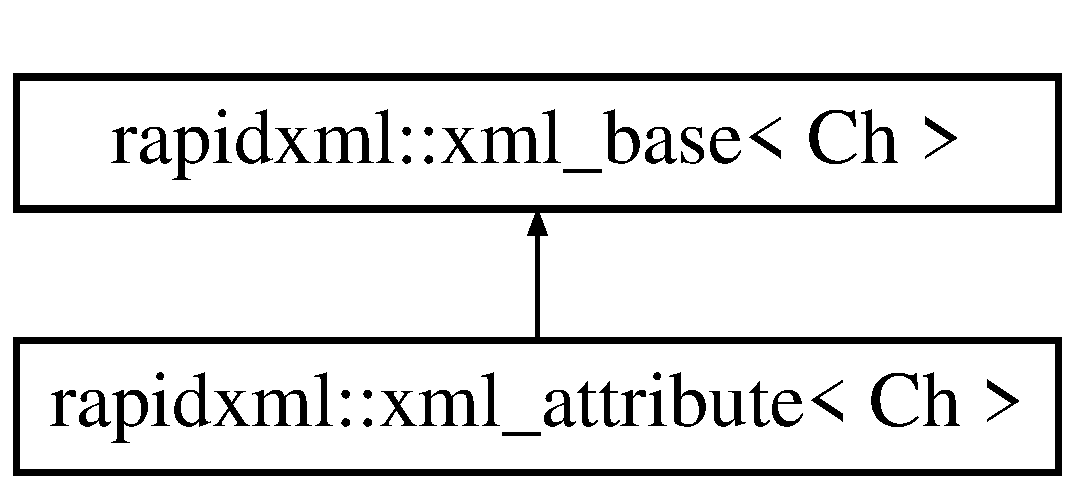
\includegraphics[height=2.000000cm]{classrapidxml_1_1xml__attribute}
\end{center}
\end{figure}
\subsection*{Public Member Functions}
\begin{DoxyCompactItemize}
\item 
\hyperlink{classrapidxml_1_1xml__attribute_a26be291103917d3e8de110d46dd83816}{xml\+\_\+attribute} ()
\item 
\hyperlink{classrapidxml_1_1xml__document}{xml\+\_\+document}$<$ Ch $>$ $\ast$ \hyperlink{classrapidxml_1_1xml__attribute_a8b6d31d899e27f01bde35b53d98496ec}{document} () const 
\item 
\hyperlink{classrapidxml_1_1xml__attribute}{xml\+\_\+attribute}$<$ Ch $>$ $\ast$ \hyperlink{classrapidxml_1_1xml__attribute_ae3547cc30b201fd6d7b98c04dda26f89}{previous\+\_\+attribute} (const Ch $\ast$\hyperlink{classrapidxml_1_1xml__base_a9a09739310469995db078ebd0da3ed45}{name}=0, std\+::size\+\_\+t \hyperlink{classrapidxml_1_1xml__base_a7e7f98b3d01e1eab8dc1ca69aad9af84}{name\+\_\+size}=0, bool case\+\_\+sensitive=true) const 
\item 
\hyperlink{classrapidxml_1_1xml__attribute}{xml\+\_\+attribute}$<$ Ch $>$ $\ast$ \hyperlink{classrapidxml_1_1xml__attribute_a56c08d7c96203286c889a43849328a86}{next\+\_\+attribute} (const Ch $\ast$\hyperlink{classrapidxml_1_1xml__base_a9a09739310469995db078ebd0da3ed45}{name}=0, std\+::size\+\_\+t \hyperlink{classrapidxml_1_1xml__base_a7e7f98b3d01e1eab8dc1ca69aad9af84}{name\+\_\+size}=0, bool case\+\_\+sensitive=true) const 
\end{DoxyCompactItemize}
\subsection*{Friends}
\begin{DoxyCompactItemize}
\item 
class \hyperlink{classrapidxml_1_1xml__attribute_aa7e464ce3fe512598ff8dda47291941f}{xml\+\_\+node$<$ Ch $>$}
\end{DoxyCompactItemize}
\subsection*{Additional Inherited Members}


\subsection{Detailed Description}
\subsubsection*{template$<$class Ch = char$>$class rapidxml\+::xml\+\_\+attribute$<$ Ch $>$}

Class representing attribute node of X\+M\+L document. 

Each attribute has name and value strings, which are available through \hyperlink{classrapidxml_1_1xml__base_a9a09739310469995db078ebd0da3ed45}{name()} and \hyperlink{classrapidxml_1_1xml__base_adcdaccff61c665f039d9344e447b7445}{value()} functions (inherited from \hyperlink{classrapidxml_1_1xml__base}{xml\+\_\+base}). Note that after parse, both name and value of attribute will point to interior of source text used for parsing. Thus, this text must persist in memory for the lifetime of attribute. 
\begin{DoxyParams}{Parameters}
{\em Ch} & Character type to use. \\
\hline
\end{DoxyParams}


\subsection{Constructor \& Destructor Documentation}
\hypertarget{classrapidxml_1_1xml__attribute_a26be291103917d3e8de110d46dd83816}{}\index{rapidxml\+::xml\+\_\+attribute@{rapidxml\+::xml\+\_\+attribute}!xml\+\_\+attribute@{xml\+\_\+attribute}}
\index{xml\+\_\+attribute@{xml\+\_\+attribute}!rapidxml\+::xml\+\_\+attribute@{rapidxml\+::xml\+\_\+attribute}}
\subsubsection[{xml\+\_\+attribute()}]{\setlength{\rightskip}{0pt plus 5cm}template$<$class Ch = char$>$ {\bf rapidxml\+::xml\+\_\+attribute}$<$ Ch $>$\+::{\bf xml\+\_\+attribute} (
\begin{DoxyParamCaption}
{}
\end{DoxyParamCaption}
)\hspace{0.3cm}{\ttfamily [inline]}}\label{classrapidxml_1_1xml__attribute_a26be291103917d3e8de110d46dd83816}
Constructs an empty attribute with the specified type. Consider using \hyperlink{classrapidxml_1_1memory__pool}{memory\+\_\+pool} of appropriate \hyperlink{classrapidxml_1_1xml__document}{xml\+\_\+document} if allocating attributes manually. 

\subsection{Member Function Documentation}
\hypertarget{classrapidxml_1_1xml__attribute_a8b6d31d899e27f01bde35b53d98496ec}{}\index{rapidxml\+::xml\+\_\+attribute@{rapidxml\+::xml\+\_\+attribute}!document@{document}}
\index{document@{document}!rapidxml\+::xml\+\_\+attribute@{rapidxml\+::xml\+\_\+attribute}}
\subsubsection[{document() const }]{\setlength{\rightskip}{0pt plus 5cm}template$<$class Ch = char$>$ {\bf xml\+\_\+document}$<$Ch$>$$\ast$ {\bf rapidxml\+::xml\+\_\+attribute}$<$ Ch $>$\+::document (
\begin{DoxyParamCaption}
{}
\end{DoxyParamCaption}
) const\hspace{0.3cm}{\ttfamily [inline]}}\label{classrapidxml_1_1xml__attribute_a8b6d31d899e27f01bde35b53d98496ec}
Gets document of which attribute is a child. \begin{DoxyReturn}{Returns}
Pointer to document that contains this attribute, or 0 if there is no parent document. 
\end{DoxyReturn}
\hypertarget{classrapidxml_1_1xml__attribute_a56c08d7c96203286c889a43849328a86}{}\index{rapidxml\+::xml\+\_\+attribute@{rapidxml\+::xml\+\_\+attribute}!next\+\_\+attribute@{next\+\_\+attribute}}
\index{next\+\_\+attribute@{next\+\_\+attribute}!rapidxml\+::xml\+\_\+attribute@{rapidxml\+::xml\+\_\+attribute}}
\subsubsection[{next\+\_\+attribute(const Ch $\ast$name=0, std\+::size\+\_\+t name\+\_\+size=0, bool case\+\_\+sensitive=true) const }]{\setlength{\rightskip}{0pt plus 5cm}template$<$class Ch = char$>$ {\bf xml\+\_\+attribute}$<$Ch$>$$\ast$ {\bf rapidxml\+::xml\+\_\+attribute}$<$ Ch $>$\+::next\+\_\+attribute (
\begin{DoxyParamCaption}
\item[{const Ch $\ast$}]{name = {\ttfamily 0}, }
\item[{std\+::size\+\_\+t}]{name\+\_\+size = {\ttfamily 0}, }
\item[{bool}]{case\+\_\+sensitive = {\ttfamily true}}
\end{DoxyParamCaption}
) const\hspace{0.3cm}{\ttfamily [inline]}}\label{classrapidxml_1_1xml__attribute_a56c08d7c96203286c889a43849328a86}
Gets next attribute, optionally matching attribute name. 
\begin{DoxyParams}{Parameters}
{\em name} & Name of attribute to find, or 0 to return next attribute regardless of its name; this string doesn\textquotesingle{}t have to be zero-\/terminated if name\+\_\+size is non-\/zero \\
\hline
{\em name\+\_\+size} & Size of name, in characters, or 0 to have size calculated automatically from string \\
\hline
{\em case\+\_\+sensitive} & Should name comparison be case-\/sensitive; non case-\/sensitive comparison works properly only for A\+S\+C\+I\+I characters \\
\hline
\end{DoxyParams}
\begin{DoxyReturn}{Returns}
Pointer to found attribute, or 0 if not found. 
\end{DoxyReturn}
\hypertarget{classrapidxml_1_1xml__attribute_ae3547cc30b201fd6d7b98c04dda26f89}{}\index{rapidxml\+::xml\+\_\+attribute@{rapidxml\+::xml\+\_\+attribute}!previous\+\_\+attribute@{previous\+\_\+attribute}}
\index{previous\+\_\+attribute@{previous\+\_\+attribute}!rapidxml\+::xml\+\_\+attribute@{rapidxml\+::xml\+\_\+attribute}}
\subsubsection[{previous\+\_\+attribute(const Ch $\ast$name=0, std\+::size\+\_\+t name\+\_\+size=0, bool case\+\_\+sensitive=true) const }]{\setlength{\rightskip}{0pt plus 5cm}template$<$class Ch = char$>$ {\bf xml\+\_\+attribute}$<$Ch$>$$\ast$ {\bf rapidxml\+::xml\+\_\+attribute}$<$ Ch $>$\+::previous\+\_\+attribute (
\begin{DoxyParamCaption}
\item[{const Ch $\ast$}]{name = {\ttfamily 0}, }
\item[{std\+::size\+\_\+t}]{name\+\_\+size = {\ttfamily 0}, }
\item[{bool}]{case\+\_\+sensitive = {\ttfamily true}}
\end{DoxyParamCaption}
) const\hspace{0.3cm}{\ttfamily [inline]}}\label{classrapidxml_1_1xml__attribute_ae3547cc30b201fd6d7b98c04dda26f89}
Gets previous attribute, optionally matching attribute name. 
\begin{DoxyParams}{Parameters}
{\em name} & Name of attribute to find, or 0 to return previous attribute regardless of its name; this string doesn\textquotesingle{}t have to be zero-\/terminated if name\+\_\+size is non-\/zero \\
\hline
{\em name\+\_\+size} & Size of name, in characters, or 0 to have size calculated automatically from string \\
\hline
{\em case\+\_\+sensitive} & Should name comparison be case-\/sensitive; non case-\/sensitive comparison works properly only for A\+S\+C\+I\+I characters \\
\hline
\end{DoxyParams}
\begin{DoxyReturn}{Returns}
Pointer to found attribute, or 0 if not found. 
\end{DoxyReturn}


\subsection{Friends And Related Function Documentation}
\hypertarget{classrapidxml_1_1xml__attribute_aa7e464ce3fe512598ff8dda47291941f}{}\index{rapidxml\+::xml\+\_\+attribute@{rapidxml\+::xml\+\_\+attribute}!xml\+\_\+node$<$ Ch $>$@{xml\+\_\+node$<$ Ch $>$}}
\index{xml\+\_\+node$<$ Ch $>$@{xml\+\_\+node$<$ Ch $>$}!rapidxml\+::xml\+\_\+attribute@{rapidxml\+::xml\+\_\+attribute}}
\subsubsection[{xml\+\_\+node$<$ Ch $>$}]{\setlength{\rightskip}{0pt plus 5cm}template$<$class Ch = char$>$ friend class {\bf xml\+\_\+node}$<$ Ch $>$\hspace{0.3cm}{\ttfamily [friend]}}\label{classrapidxml_1_1xml__attribute_aa7e464ce3fe512598ff8dda47291941f}


The documentation for this class was generated from the following file\+:\begin{DoxyCompactItemize}
\item 
/\+Users/brandonmcfarland/\+Desktop/searchdocs/\+Search\+Engine/\+Final\+Project/\hyperlink{rapidxml_8hpp}{rapidxml.\+hpp}\end{DoxyCompactItemize}

\hypertarget{classrapidxml_1_1xml__base}{}\section{rapidxml\+:\+:xml\+\_\+base$<$ Ch $>$ Class Template Reference}
\label{classrapidxml_1_1xml__base}\index{rapidxml\+::xml\+\_\+base$<$ Ch $>$@{rapidxml\+::xml\+\_\+base$<$ Ch $>$}}


Base class for \hyperlink{classrapidxml_1_1xml__node}{xml\+\_\+node} and \hyperlink{classrapidxml_1_1xml__attribute}{xml\+\_\+attribute} implementing common functions\+: \hyperlink{classrapidxml_1_1xml__base_a9a09739310469995db078ebd0da3ed45}{name()}, \hyperlink{classrapidxml_1_1xml__base_a7e7f98b3d01e1eab8dc1ca69aad9af84}{name\+\_\+size()}, \hyperlink{classrapidxml_1_1xml__base_adcdaccff61c665f039d9344e447b7445}{value()}, \hyperlink{classrapidxml_1_1xml__base_a9fcf201ed0915ac18dd43b0b5dcfaf32}{value\+\_\+size()} and \hyperlink{classrapidxml_1_1xml__base_a7f31ae930f93852830234db1ae59c4c4}{parent()}.  




{\ttfamily \#include $<$rapidxml.\+hpp$>$}

Inheritance diagram for rapidxml\+:\+:xml\+\_\+base$<$ Ch $>$\+:\begin{figure}[H]
\begin{center}
\leavevmode
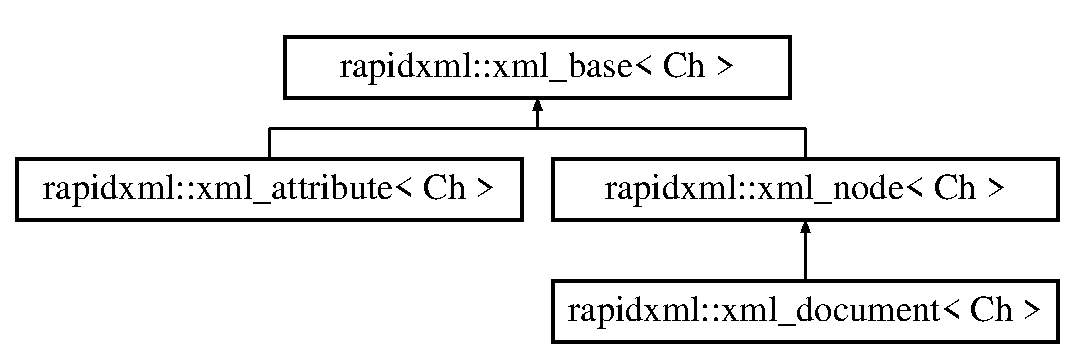
\includegraphics[height=3.000000cm]{classrapidxml_1_1xml__base}
\end{center}
\end{figure}
\subsection*{Public Member Functions}
\begin{DoxyCompactItemize}
\item 
\hyperlink{classrapidxml_1_1xml__base_a23e7f7aac02d17a0a01afb597e4b966b}{xml\+\_\+base} ()
\item 
Ch $\ast$ \hyperlink{classrapidxml_1_1xml__base_a9a09739310469995db078ebd0da3ed45}{name} () const 
\item 
std\+::size\+\_\+t \hyperlink{classrapidxml_1_1xml__base_a7e7f98b3d01e1eab8dc1ca69aad9af84}{name\+\_\+size} () const 
\item 
Ch $\ast$ \hyperlink{classrapidxml_1_1xml__base_adcdaccff61c665f039d9344e447b7445}{value} () const 
\item 
std\+::size\+\_\+t \hyperlink{classrapidxml_1_1xml__base_a9fcf201ed0915ac18dd43b0b5dcfaf32}{value\+\_\+size} () const 
\item 
void \hyperlink{classrapidxml_1_1xml__base_ae55060ae958c6e6465d6c8db852ec6ce}{name} (const Ch $\ast$name, std\+::size\+\_\+t size)
\item 
void \hyperlink{classrapidxml_1_1xml__base_a4611ddc82ac83a527c65606600eb2a0d}{name} (const Ch $\ast$name)
\item 
void \hyperlink{classrapidxml_1_1xml__base_a3b183c2db7022a6d30494dd2f0ac11e9}{value} (const Ch $\ast$value, std\+::size\+\_\+t size)
\item 
void \hyperlink{classrapidxml_1_1xml__base_a81e63ec4bfd2d7ef0a6c2ed49be6e623}{value} (const Ch $\ast$value)
\item 
\hyperlink{classrapidxml_1_1xml__node}{xml\+\_\+node}$<$ Ch $>$ $\ast$ \hyperlink{classrapidxml_1_1xml__base_a7f31ae930f93852830234db1ae59c4c4}{parent} () const 
\end{DoxyCompactItemize}
\subsection*{Static Protected Member Functions}
\begin{DoxyCompactItemize}
\item 
static Ch $\ast$ \hyperlink{classrapidxml_1_1xml__base_ad96ff6b1e41dab3ff60b9bc4df769a75}{nullstr} ()
\end{DoxyCompactItemize}
\subsection*{Protected Attributes}
\begin{DoxyCompactItemize}
\item 
Ch $\ast$ \hyperlink{classrapidxml_1_1xml__base_afd9851ed43e14619db0d7075ef8e9e8a}{m\+\_\+name}
\item 
Ch $\ast$ \hyperlink{classrapidxml_1_1xml__base_a278a1ea63b0b70219b946cec47fa00ea}{m\+\_\+value}
\item 
std\+::size\+\_\+t \hyperlink{classrapidxml_1_1xml__base_a5a8c76a7274b4180213796422c4df76f}{m\+\_\+name\+\_\+size}
\item 
std\+::size\+\_\+t \hyperlink{classrapidxml_1_1xml__base_aa3a49d8ceddb8a8d7edb773a2226b89c}{m\+\_\+value\+\_\+size}
\item 
\hyperlink{classrapidxml_1_1xml__node}{xml\+\_\+node}$<$ Ch $>$ $\ast$ \hyperlink{classrapidxml_1_1xml__base_a90d5f660f078f66563fd7b2d8387ccb0}{m\+\_\+parent}
\end{DoxyCompactItemize}


\subsection{Detailed Description}
\subsubsection*{template$<$class Ch = char$>$class rapidxml\+::xml\+\_\+base$<$ Ch $>$}

Base class for \hyperlink{classrapidxml_1_1xml__node}{xml\+\_\+node} and \hyperlink{classrapidxml_1_1xml__attribute}{xml\+\_\+attribute} implementing common functions\+: \hyperlink{classrapidxml_1_1xml__base_a9a09739310469995db078ebd0da3ed45}{name()}, \hyperlink{classrapidxml_1_1xml__base_a7e7f98b3d01e1eab8dc1ca69aad9af84}{name\+\_\+size()}, \hyperlink{classrapidxml_1_1xml__base_adcdaccff61c665f039d9344e447b7445}{value()}, \hyperlink{classrapidxml_1_1xml__base_a9fcf201ed0915ac18dd43b0b5dcfaf32}{value\+\_\+size()} and \hyperlink{classrapidxml_1_1xml__base_a7f31ae930f93852830234db1ae59c4c4}{parent()}. 

Base class for \hyperlink{classrapidxml_1_1xml__node}{xml\+\_\+node} and \hyperlink{classrapidxml_1_1xml__attribute}{xml\+\_\+attribute} implementing common functions\+: \hyperlink{classrapidxml_1_1xml__base_a9a09739310469995db078ebd0da3ed45}{name()}, \hyperlink{classrapidxml_1_1xml__base_a7e7f98b3d01e1eab8dc1ca69aad9af84}{name\+\_\+size()}, \hyperlink{classrapidxml_1_1xml__base_adcdaccff61c665f039d9344e447b7445}{value()}, \hyperlink{classrapidxml_1_1xml__base_a9fcf201ed0915ac18dd43b0b5dcfaf32}{value\+\_\+size()} and \hyperlink{classrapidxml_1_1xml__base_a7f31ae930f93852830234db1ae59c4c4}{parent()}. 
\begin{DoxyParams}{Parameters}
{\em Ch} & Character type to use \\
\hline
\end{DoxyParams}


\subsection{Constructor \& Destructor Documentation}
\hypertarget{classrapidxml_1_1xml__base_a23e7f7aac02d17a0a01afb597e4b966b}{}\index{rapidxml\+::xml\+\_\+base@{rapidxml\+::xml\+\_\+base}!xml\+\_\+base@{xml\+\_\+base}}
\index{xml\+\_\+base@{xml\+\_\+base}!rapidxml\+::xml\+\_\+base@{rapidxml\+::xml\+\_\+base}}
\subsubsection[{xml\+\_\+base()}]{\setlength{\rightskip}{0pt plus 5cm}template$<$class Ch  = char$>$ {\bf rapidxml\+::xml\+\_\+base}$<$ Ch $>$\+::{\bf xml\+\_\+base} (
\begin{DoxyParamCaption}
{}
\end{DoxyParamCaption}
)\hspace{0.3cm}{\ttfamily [inline]}}\label{classrapidxml_1_1xml__base_a23e7f7aac02d17a0a01afb597e4b966b}


\subsection{Member Function Documentation}
\hypertarget{classrapidxml_1_1xml__base_a9a09739310469995db078ebd0da3ed45}{}\index{rapidxml\+::xml\+\_\+base@{rapidxml\+::xml\+\_\+base}!name@{name}}
\index{name@{name}!rapidxml\+::xml\+\_\+base@{rapidxml\+::xml\+\_\+base}}
\subsubsection[{name() const }]{\setlength{\rightskip}{0pt plus 5cm}template$<$class Ch  = char$>$ Ch$\ast$ {\bf rapidxml\+::xml\+\_\+base}$<$ Ch $>$\+::name (
\begin{DoxyParamCaption}
{}
\end{DoxyParamCaption}
) const\hspace{0.3cm}{\ttfamily [inline]}}\label{classrapidxml_1_1xml__base_a9a09739310469995db078ebd0da3ed45}
Gets name of the node. Interpretation of name depends on type of node. Note that name will not be zero-\/terminated if \hyperlink{namespacerapidxml_af3fc88ba6bee33482a2db81b1da36ea1}{rapidxml\+::parse\+\_\+no\+\_\+string\+\_\+terminators} option was selected during parse. ~\newline
~\newline
 Use \hyperlink{classrapidxml_1_1xml__base_a7e7f98b3d01e1eab8dc1ca69aad9af84}{name\+\_\+size()} function to determine length of the name. \begin{DoxyReturn}{Returns}
Name of node, or empty string if node has no name. 
\end{DoxyReturn}
\hypertarget{classrapidxml_1_1xml__base_ae55060ae958c6e6465d6c8db852ec6ce}{}\index{rapidxml\+::xml\+\_\+base@{rapidxml\+::xml\+\_\+base}!name@{name}}
\index{name@{name}!rapidxml\+::xml\+\_\+base@{rapidxml\+::xml\+\_\+base}}
\subsubsection[{name(const Ch $\ast$name, std\+::size\+\_\+t size)}]{\setlength{\rightskip}{0pt plus 5cm}template$<$class Ch  = char$>$ void {\bf rapidxml\+::xml\+\_\+base}$<$ Ch $>$\+::name (
\begin{DoxyParamCaption}
\item[{const Ch $\ast$}]{name, }
\item[{std\+::size\+\_\+t}]{size}
\end{DoxyParamCaption}
)\hspace{0.3cm}{\ttfamily [inline]}}\label{classrapidxml_1_1xml__base_ae55060ae958c6e6465d6c8db852ec6ce}
Sets name of node to a non zero-\/terminated string. See ownership\+\_\+of\+\_\+strings. ~\newline
~\newline
 Note that node does not own its name or value, it only stores a pointer to it. It will not delete or otherwise free the pointer on destruction. It is reponsibility of the user to properly manage lifetime of the string. The easiest way to achieve it is to use \hyperlink{classrapidxml_1_1memory__pool}{memory\+\_\+pool} of the document to allocate the string -\/ on destruction of the document the string will be automatically freed. ~\newline
~\newline
 Size of name must be specified separately, because name does not have to be zero terminated. Use \hyperlink{classrapidxml_1_1xml__base_a4611ddc82ac83a527c65606600eb2a0d}{name(const Ch $\ast$)} function to have the length automatically calculated (string must be zero terminated). 
\begin{DoxyParams}{Parameters}
{\em name} & Name of node to set. Does not have to be zero terminated. \\
\hline
{\em size} & Size of name, in characters. This does not include zero terminator, if one is present. \\
\hline
\end{DoxyParams}
\hypertarget{classrapidxml_1_1xml__base_a4611ddc82ac83a527c65606600eb2a0d}{}\index{rapidxml\+::xml\+\_\+base@{rapidxml\+::xml\+\_\+base}!name@{name}}
\index{name@{name}!rapidxml\+::xml\+\_\+base@{rapidxml\+::xml\+\_\+base}}
\subsubsection[{name(const Ch $\ast$name)}]{\setlength{\rightskip}{0pt plus 5cm}template$<$class Ch  = char$>$ void {\bf rapidxml\+::xml\+\_\+base}$<$ Ch $>$\+::name (
\begin{DoxyParamCaption}
\item[{const Ch $\ast$}]{name}
\end{DoxyParamCaption}
)\hspace{0.3cm}{\ttfamily [inline]}}\label{classrapidxml_1_1xml__base_a4611ddc82ac83a527c65606600eb2a0d}
Sets name of node to a zero-\/terminated string. See also ownership\+\_\+of\+\_\+strings and \hyperlink{classrapidxml_1_1xml__base_ae55060ae958c6e6465d6c8db852ec6ce}{xml\+\_\+node\+::name(const Ch $\ast$, std\+::size\+\_\+t)}. 
\begin{DoxyParams}{Parameters}
{\em name} & Name of node to set. Must be zero terminated. \\
\hline
\end{DoxyParams}
\hypertarget{classrapidxml_1_1xml__base_a7e7f98b3d01e1eab8dc1ca69aad9af84}{}\index{rapidxml\+::xml\+\_\+base@{rapidxml\+::xml\+\_\+base}!name\+\_\+size@{name\+\_\+size}}
\index{name\+\_\+size@{name\+\_\+size}!rapidxml\+::xml\+\_\+base@{rapidxml\+::xml\+\_\+base}}
\subsubsection[{name\+\_\+size() const }]{\setlength{\rightskip}{0pt plus 5cm}template$<$class Ch  = char$>$ std\+::size\+\_\+t {\bf rapidxml\+::xml\+\_\+base}$<$ Ch $>$\+::name\+\_\+size (
\begin{DoxyParamCaption}
{}
\end{DoxyParamCaption}
) const\hspace{0.3cm}{\ttfamily [inline]}}\label{classrapidxml_1_1xml__base_a7e7f98b3d01e1eab8dc1ca69aad9af84}
Gets size of node name, not including terminator character. This function works correctly irrespective of whether name is or is not zero terminated. \begin{DoxyReturn}{Returns}
Size of node name, in characters. 
\end{DoxyReturn}
\hypertarget{classrapidxml_1_1xml__base_ad96ff6b1e41dab3ff60b9bc4df769a75}{}\index{rapidxml\+::xml\+\_\+base@{rapidxml\+::xml\+\_\+base}!nullstr@{nullstr}}
\index{nullstr@{nullstr}!rapidxml\+::xml\+\_\+base@{rapidxml\+::xml\+\_\+base}}
\subsubsection[{nullstr()}]{\setlength{\rightskip}{0pt plus 5cm}template$<$class Ch  = char$>$ static Ch$\ast$ {\bf rapidxml\+::xml\+\_\+base}$<$ Ch $>$\+::nullstr (
\begin{DoxyParamCaption}
{}
\end{DoxyParamCaption}
)\hspace{0.3cm}{\ttfamily [inline]}, {\ttfamily [static]}, {\ttfamily [protected]}}\label{classrapidxml_1_1xml__base_ad96ff6b1e41dab3ff60b9bc4df769a75}
\hypertarget{classrapidxml_1_1xml__base_a7f31ae930f93852830234db1ae59c4c4}{}\index{rapidxml\+::xml\+\_\+base@{rapidxml\+::xml\+\_\+base}!parent@{parent}}
\index{parent@{parent}!rapidxml\+::xml\+\_\+base@{rapidxml\+::xml\+\_\+base}}
\subsubsection[{parent() const }]{\setlength{\rightskip}{0pt plus 5cm}template$<$class Ch  = char$>$ {\bf xml\+\_\+node}$<$Ch$>$$\ast$ {\bf rapidxml\+::xml\+\_\+base}$<$ Ch $>$\+::parent (
\begin{DoxyParamCaption}
{}
\end{DoxyParamCaption}
) const\hspace{0.3cm}{\ttfamily [inline]}}\label{classrapidxml_1_1xml__base_a7f31ae930f93852830234db1ae59c4c4}
Gets node parent. \begin{DoxyReturn}{Returns}
Pointer to parent node, or 0 if there is no parent. 
\end{DoxyReturn}
\hypertarget{classrapidxml_1_1xml__base_adcdaccff61c665f039d9344e447b7445}{}\index{rapidxml\+::xml\+\_\+base@{rapidxml\+::xml\+\_\+base}!value@{value}}
\index{value@{value}!rapidxml\+::xml\+\_\+base@{rapidxml\+::xml\+\_\+base}}
\subsubsection[{value() const }]{\setlength{\rightskip}{0pt plus 5cm}template$<$class Ch  = char$>$ Ch$\ast$ {\bf rapidxml\+::xml\+\_\+base}$<$ Ch $>$\+::value (
\begin{DoxyParamCaption}
{}
\end{DoxyParamCaption}
) const\hspace{0.3cm}{\ttfamily [inline]}}\label{classrapidxml_1_1xml__base_adcdaccff61c665f039d9344e447b7445}
Gets value of node. Interpretation of value depends on type of node. Note that value will not be zero-\/terminated if \hyperlink{namespacerapidxml_af3fc88ba6bee33482a2db81b1da36ea1}{rapidxml\+::parse\+\_\+no\+\_\+string\+\_\+terminators} option was selected during parse. ~\newline
~\newline
 Use \hyperlink{classrapidxml_1_1xml__base_a9fcf201ed0915ac18dd43b0b5dcfaf32}{value\+\_\+size()} function to determine length of the value. \begin{DoxyReturn}{Returns}
Value of node, or empty string if node has no value. 
\end{DoxyReturn}
\hypertarget{classrapidxml_1_1xml__base_a3b183c2db7022a6d30494dd2f0ac11e9}{}\index{rapidxml\+::xml\+\_\+base@{rapidxml\+::xml\+\_\+base}!value@{value}}
\index{value@{value}!rapidxml\+::xml\+\_\+base@{rapidxml\+::xml\+\_\+base}}
\subsubsection[{value(const Ch $\ast$value, std\+::size\+\_\+t size)}]{\setlength{\rightskip}{0pt plus 5cm}template$<$class Ch  = char$>$ void {\bf rapidxml\+::xml\+\_\+base}$<$ Ch $>$\+::value (
\begin{DoxyParamCaption}
\item[{const Ch $\ast$}]{value, }
\item[{std\+::size\+\_\+t}]{size}
\end{DoxyParamCaption}
)\hspace{0.3cm}{\ttfamily [inline]}}\label{classrapidxml_1_1xml__base_a3b183c2db7022a6d30494dd2f0ac11e9}
Sets value of node to a non zero-\/terminated string. See ownership\+\_\+of\+\_\+strings. ~\newline
~\newline
 Note that node does not own its name or value, it only stores a pointer to it. It will not delete or otherwise free the pointer on destruction. It is reponsibility of the user to properly manage lifetime of the string. The easiest way to achieve it is to use \hyperlink{classrapidxml_1_1memory__pool}{memory\+\_\+pool} of the document to allocate the string -\/ on destruction of the document the string will be automatically freed. ~\newline
~\newline
 Size of value must be specified separately, because it does not have to be zero terminated. Use \hyperlink{classrapidxml_1_1xml__base_a81e63ec4bfd2d7ef0a6c2ed49be6e623}{value(const Ch $\ast$)} function to have the length automatically calculated (string must be zero terminated). ~\newline
~\newline
 If an element has a child node of type node\+\_\+data, it will take precedence over element value when printing. If you want to manipulate data of elements using values, use parser flag \hyperlink{namespacerapidxml_ac2d21ef14a4e8936b94aca5d38b1a74d}{rapidxml\+::parse\+\_\+no\+\_\+data\+\_\+nodes} to prevent creation of data nodes by the parser. 
\begin{DoxyParams}{Parameters}
{\em value} & value of node to set. Does not have to be zero terminated. \\
\hline
{\em size} & Size of value, in characters. This does not include zero terminator, if one is present. \\
\hline
\end{DoxyParams}
\hypertarget{classrapidxml_1_1xml__base_a81e63ec4bfd2d7ef0a6c2ed49be6e623}{}\index{rapidxml\+::xml\+\_\+base@{rapidxml\+::xml\+\_\+base}!value@{value}}
\index{value@{value}!rapidxml\+::xml\+\_\+base@{rapidxml\+::xml\+\_\+base}}
\subsubsection[{value(const Ch $\ast$value)}]{\setlength{\rightskip}{0pt plus 5cm}template$<$class Ch  = char$>$ void {\bf rapidxml\+::xml\+\_\+base}$<$ Ch $>$\+::value (
\begin{DoxyParamCaption}
\item[{const Ch $\ast$}]{value}
\end{DoxyParamCaption}
)\hspace{0.3cm}{\ttfamily [inline]}}\label{classrapidxml_1_1xml__base_a81e63ec4bfd2d7ef0a6c2ed49be6e623}
Sets value of node to a zero-\/terminated string. See also ownership\+\_\+of\+\_\+strings and \hyperlink{classrapidxml_1_1xml__base_a3b183c2db7022a6d30494dd2f0ac11e9}{xml\+\_\+node\+::value(const Ch $\ast$, std\+::size\+\_\+t)}. 
\begin{DoxyParams}{Parameters}
{\em value} & Vame of node to set. Must be zero terminated. \\
\hline
\end{DoxyParams}
\hypertarget{classrapidxml_1_1xml__base_a9fcf201ed0915ac18dd43b0b5dcfaf32}{}\index{rapidxml\+::xml\+\_\+base@{rapidxml\+::xml\+\_\+base}!value\+\_\+size@{value\+\_\+size}}
\index{value\+\_\+size@{value\+\_\+size}!rapidxml\+::xml\+\_\+base@{rapidxml\+::xml\+\_\+base}}
\subsubsection[{value\+\_\+size() const }]{\setlength{\rightskip}{0pt plus 5cm}template$<$class Ch  = char$>$ std\+::size\+\_\+t {\bf rapidxml\+::xml\+\_\+base}$<$ Ch $>$\+::value\+\_\+size (
\begin{DoxyParamCaption}
{}
\end{DoxyParamCaption}
) const\hspace{0.3cm}{\ttfamily [inline]}}\label{classrapidxml_1_1xml__base_a9fcf201ed0915ac18dd43b0b5dcfaf32}
Gets size of node value, not including terminator character. This function works correctly irrespective of whether value is or is not zero terminated. \begin{DoxyReturn}{Returns}
Size of node value, in characters. 
\end{DoxyReturn}


\subsection{Member Data Documentation}
\hypertarget{classrapidxml_1_1xml__base_afd9851ed43e14619db0d7075ef8e9e8a}{}\index{rapidxml\+::xml\+\_\+base@{rapidxml\+::xml\+\_\+base}!m\+\_\+name@{m\+\_\+name}}
\index{m\+\_\+name@{m\+\_\+name}!rapidxml\+::xml\+\_\+base@{rapidxml\+::xml\+\_\+base}}
\subsubsection[{m\+\_\+name}]{\setlength{\rightskip}{0pt plus 5cm}template$<$class Ch  = char$>$ Ch$\ast$ {\bf rapidxml\+::xml\+\_\+base}$<$ Ch $>$\+::m\+\_\+name\hspace{0.3cm}{\ttfamily [protected]}}\label{classrapidxml_1_1xml__base_afd9851ed43e14619db0d7075ef8e9e8a}
\hypertarget{classrapidxml_1_1xml__base_a5a8c76a7274b4180213796422c4df76f}{}\index{rapidxml\+::xml\+\_\+base@{rapidxml\+::xml\+\_\+base}!m\+\_\+name\+\_\+size@{m\+\_\+name\+\_\+size}}
\index{m\+\_\+name\+\_\+size@{m\+\_\+name\+\_\+size}!rapidxml\+::xml\+\_\+base@{rapidxml\+::xml\+\_\+base}}
\subsubsection[{m\+\_\+name\+\_\+size}]{\setlength{\rightskip}{0pt plus 5cm}template$<$class Ch  = char$>$ std\+::size\+\_\+t {\bf rapidxml\+::xml\+\_\+base}$<$ Ch $>$\+::m\+\_\+name\+\_\+size\hspace{0.3cm}{\ttfamily [protected]}}\label{classrapidxml_1_1xml__base_a5a8c76a7274b4180213796422c4df76f}
\hypertarget{classrapidxml_1_1xml__base_a90d5f660f078f66563fd7b2d8387ccb0}{}\index{rapidxml\+::xml\+\_\+base@{rapidxml\+::xml\+\_\+base}!m\+\_\+parent@{m\+\_\+parent}}
\index{m\+\_\+parent@{m\+\_\+parent}!rapidxml\+::xml\+\_\+base@{rapidxml\+::xml\+\_\+base}}
\subsubsection[{m\+\_\+parent}]{\setlength{\rightskip}{0pt plus 5cm}template$<$class Ch  = char$>$ {\bf xml\+\_\+node}$<$Ch$>$$\ast$ {\bf rapidxml\+::xml\+\_\+base}$<$ Ch $>$\+::m\+\_\+parent\hspace{0.3cm}{\ttfamily [protected]}}\label{classrapidxml_1_1xml__base_a90d5f660f078f66563fd7b2d8387ccb0}
\hypertarget{classrapidxml_1_1xml__base_a278a1ea63b0b70219b946cec47fa00ea}{}\index{rapidxml\+::xml\+\_\+base@{rapidxml\+::xml\+\_\+base}!m\+\_\+value@{m\+\_\+value}}
\index{m\+\_\+value@{m\+\_\+value}!rapidxml\+::xml\+\_\+base@{rapidxml\+::xml\+\_\+base}}
\subsubsection[{m\+\_\+value}]{\setlength{\rightskip}{0pt plus 5cm}template$<$class Ch  = char$>$ Ch$\ast$ {\bf rapidxml\+::xml\+\_\+base}$<$ Ch $>$\+::m\+\_\+value\hspace{0.3cm}{\ttfamily [protected]}}\label{classrapidxml_1_1xml__base_a278a1ea63b0b70219b946cec47fa00ea}
\hypertarget{classrapidxml_1_1xml__base_aa3a49d8ceddb8a8d7edb773a2226b89c}{}\index{rapidxml\+::xml\+\_\+base@{rapidxml\+::xml\+\_\+base}!m\+\_\+value\+\_\+size@{m\+\_\+value\+\_\+size}}
\index{m\+\_\+value\+\_\+size@{m\+\_\+value\+\_\+size}!rapidxml\+::xml\+\_\+base@{rapidxml\+::xml\+\_\+base}}
\subsubsection[{m\+\_\+value\+\_\+size}]{\setlength{\rightskip}{0pt plus 5cm}template$<$class Ch  = char$>$ std\+::size\+\_\+t {\bf rapidxml\+::xml\+\_\+base}$<$ Ch $>$\+::m\+\_\+value\+\_\+size\hspace{0.3cm}{\ttfamily [protected]}}\label{classrapidxml_1_1xml__base_aa3a49d8ceddb8a8d7edb773a2226b89c}


The documentation for this class was generated from the following file\+:\begin{DoxyCompactItemize}
\item 
/\+Users/brandonmcfarland/\+Desktop/searchdocs/\+Search\+Engine/\+Final\+Project/\hyperlink{rapidxml_8hpp}{rapidxml.\+hpp}\end{DoxyCompactItemize}

\hypertarget{classrapidxml_1_1xml__document}{}\section{rapidxml\+:\+:xml\+\_\+document$<$ Ch $>$ Class Template Reference}
\label{classrapidxml_1_1xml__document}\index{rapidxml\+::xml\+\_\+document$<$ Ch $>$@{rapidxml\+::xml\+\_\+document$<$ Ch $>$}}


X\+M\+L document.  




{\ttfamily \#include $<$rapidxml.\+hpp$>$}

Inheritance diagram for rapidxml\+:\+:xml\+\_\+document$<$ Ch $>$\+:\begin{figure}[H]
\begin{center}
\leavevmode
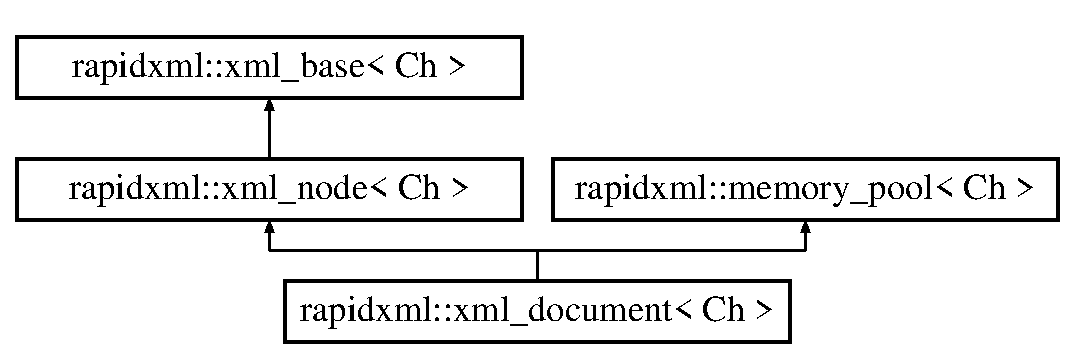
\includegraphics[height=3.000000cm]{classrapidxml_1_1xml__document}
\end{center}
\end{figure}
\subsection*{Public Member Functions}
\begin{DoxyCompactItemize}
\item 
\hyperlink{classrapidxml_1_1xml__document_aae8841b15085ba8f32ff46587ace28f5}{xml\+\_\+document} ()
\begin{DoxyCompactList}\small\item\em Constructs empty X\+M\+L document. \end{DoxyCompactList}\item 
{\footnotesize template$<$int Flags$>$ }\\void \hyperlink{classrapidxml_1_1xml__document_ac6e73ff9ac323bf5a370c38feb03a6b1}{parse} (Ch $\ast$text)
\item 
void \hyperlink{classrapidxml_1_1xml__document_a826929ff54242532198701f19ff5f83f}{clear} ()
\end{DoxyCompactItemize}
\subsection*{Additional Inherited Members}


\subsection{Detailed Description}
\subsubsection*{template$<$class Ch = char$>$class rapidxml\+::xml\+\_\+document$<$ Ch $>$}

X\+M\+L document. 

This class represents root of the D\+O\+M hierarchy. It is also an \hyperlink{classrapidxml_1_1xml__node}{xml\+\_\+node} and a \hyperlink{classrapidxml_1_1memory__pool}{memory\+\_\+pool} through public inheritance. Use \hyperlink{classrapidxml_1_1xml__document_ac6e73ff9ac323bf5a370c38feb03a6b1}{parse()} function to build a D\+O\+M tree from a zero-\/terminated X\+M\+L text string. \hyperlink{classrapidxml_1_1xml__document_ac6e73ff9ac323bf5a370c38feb03a6b1}{parse()} function allocates memory for nodes and attributes by using functions of \hyperlink{classrapidxml_1_1xml__document}{xml\+\_\+document}, which are inherited from \hyperlink{classrapidxml_1_1memory__pool}{memory\+\_\+pool}. To access root node of the document, use the document itself, as if it was an \hyperlink{classrapidxml_1_1xml__node}{xml\+\_\+node}. 
\begin{DoxyParams}{Parameters}
{\em Ch} & Character type to use. \\
\hline
\end{DoxyParams}


\subsection{Constructor \& Destructor Documentation}
\hypertarget{classrapidxml_1_1xml__document_aae8841b15085ba8f32ff46587ace28f5}{}\index{rapidxml\+::xml\+\_\+document@{rapidxml\+::xml\+\_\+document}!xml\+\_\+document@{xml\+\_\+document}}
\index{xml\+\_\+document@{xml\+\_\+document}!rapidxml\+::xml\+\_\+document@{rapidxml\+::xml\+\_\+document}}
\subsubsection[{xml\+\_\+document()}]{\setlength{\rightskip}{0pt plus 5cm}template$<$class Ch  = char$>$ {\bf rapidxml\+::xml\+\_\+document}$<$ Ch $>$\+::{\bf xml\+\_\+document} (
\begin{DoxyParamCaption}
{}
\end{DoxyParamCaption}
)\hspace{0.3cm}{\ttfamily [inline]}}\label{classrapidxml_1_1xml__document_aae8841b15085ba8f32ff46587ace28f5}


Constructs empty X\+M\+L document. 



\subsection{Member Function Documentation}
\hypertarget{classrapidxml_1_1xml__document_a826929ff54242532198701f19ff5f83f}{}\index{rapidxml\+::xml\+\_\+document@{rapidxml\+::xml\+\_\+document}!clear@{clear}}
\index{clear@{clear}!rapidxml\+::xml\+\_\+document@{rapidxml\+::xml\+\_\+document}}
\subsubsection[{clear()}]{\setlength{\rightskip}{0pt plus 5cm}template$<$class Ch  = char$>$ void {\bf rapidxml\+::xml\+\_\+document}$<$ Ch $>$\+::clear (
\begin{DoxyParamCaption}
{}
\end{DoxyParamCaption}
)\hspace{0.3cm}{\ttfamily [inline]}}\label{classrapidxml_1_1xml__document_a826929ff54242532198701f19ff5f83f}
Clears the document by deleting all nodes and clearing the memory pool. All nodes owned by document pool are destroyed. \hypertarget{classrapidxml_1_1xml__document_ac6e73ff9ac323bf5a370c38feb03a6b1}{}\index{rapidxml\+::xml\+\_\+document@{rapidxml\+::xml\+\_\+document}!parse@{parse}}
\index{parse@{parse}!rapidxml\+::xml\+\_\+document@{rapidxml\+::xml\+\_\+document}}
\subsubsection[{parse(\+Ch $\ast$text)}]{\setlength{\rightskip}{0pt plus 5cm}template$<$class Ch  = char$>$ template$<$int Flags$>$ void {\bf rapidxml\+::xml\+\_\+document}$<$ Ch $>$\+::parse (
\begin{DoxyParamCaption}
\item[{Ch $\ast$}]{text}
\end{DoxyParamCaption}
)\hspace{0.3cm}{\ttfamily [inline]}}\label{classrapidxml_1_1xml__document_ac6e73ff9ac323bf5a370c38feb03a6b1}
Parses zero-\/terminated X\+M\+L string according to given flags. Passed string will be modified by the parser, unless \hyperlink{namespacerapidxml_a45d4d8fef551beaaba23a83b847fd6a3}{rapidxml\+::parse\+\_\+non\+\_\+destructive} flag is used. The string must persist for the lifetime of the document. In case of error, \hyperlink{classrapidxml_1_1parse__error}{rapidxml\+::parse\+\_\+error} exception will be thrown. ~\newline
~\newline
 If you want to parse contents of a file, you must first load the file into the memory, and pass pointer to its beginning. Make sure that data is zero-\/terminated. ~\newline
~\newline
 Document can be parsed into multiple times. Each new call to parse removes previous nodes and attributes (if any), but does not clear memory pool. 
\begin{DoxyParams}{Parameters}
{\em text} & X\+M\+L data to parse; pointer is non-\/const to denote fact that this data may be modified by the parser. \\
\hline
\end{DoxyParams}


The documentation for this class was generated from the following file\+:\begin{DoxyCompactItemize}
\item 
/\+Users/brandonmcfarland/\+Desktop/searchdocs/\+Search\+Engine/\+Final\+Project/\hyperlink{rapidxml_8hpp}{rapidxml.\+hpp}\end{DoxyCompactItemize}

\hypertarget{classrapidxml_1_1xml__node}{}\section{rapidxml\+:\+:xml\+\_\+node$<$ Ch $>$ Class Template Reference}
\label{classrapidxml_1_1xml__node}\index{rapidxml\+::xml\+\_\+node$<$ Ch $>$@{rapidxml\+::xml\+\_\+node$<$ Ch $>$}}


Class representing a node of X\+M\+L document.  




{\ttfamily \#include $<$rapidxml.\+hpp$>$}

Inheritance diagram for rapidxml\+:\+:xml\+\_\+node$<$ Ch $>$\+:\begin{figure}[H]
\begin{center}
\leavevmode
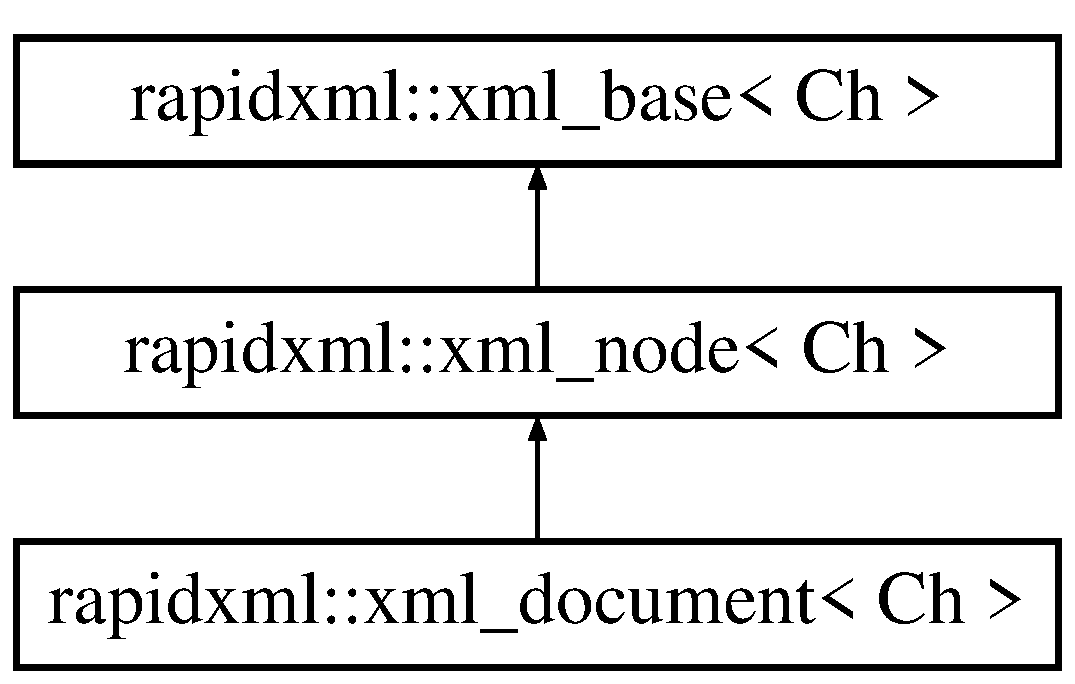
\includegraphics[height=3.000000cm]{classrapidxml_1_1xml__node}
\end{center}
\end{figure}
\subsection*{Public Member Functions}
\begin{DoxyCompactItemize}
\item 
\hyperlink{classrapidxml_1_1xml__node_a8bd9019960b90605a45998b661fb1b0e}{xml\+\_\+node} (\hyperlink{namespacerapidxml_abb456db38f7efb746c4330eed6072a7c}{node\+\_\+type} \hyperlink{classrapidxml_1_1xml__node_a2c6a4315b98bcfa2e04fed3fa1b22c36}{type})
\item 
\hyperlink{namespacerapidxml_abb456db38f7efb746c4330eed6072a7c}{node\+\_\+type} \hyperlink{classrapidxml_1_1xml__node_a2c6a4315b98bcfa2e04fed3fa1b22c36}{type} () const 
\item 
\hyperlink{classrapidxml_1_1xml__document}{xml\+\_\+document}$<$ Ch $>$ $\ast$ \hyperlink{classrapidxml_1_1xml__node_adb6ad21a4590cf13d4a6a5036e3cdbbc}{document} () const 
\item 
\hyperlink{classrapidxml_1_1xml__node}{xml\+\_\+node}$<$ Ch $>$ $\ast$ \hyperlink{classrapidxml_1_1xml__node_a2dedeb4e04bb35e06a9a7bddf6ba652d}{first\+\_\+node} (const Ch $\ast$\hyperlink{classrapidxml_1_1xml__base_a9a09739310469995db078ebd0da3ed45}{name}=0, std\+::size\+\_\+t \hyperlink{classrapidxml_1_1xml__base_a7e7f98b3d01e1eab8dc1ca69aad9af84}{name\+\_\+size}=0, bool case\+\_\+sensitive=true) const 
\item 
\hyperlink{classrapidxml_1_1xml__node}{xml\+\_\+node}$<$ Ch $>$ $\ast$ \hyperlink{classrapidxml_1_1xml__node_a2ace550c18cf10da6303773972d7157f}{last\+\_\+node} (const Ch $\ast$\hyperlink{classrapidxml_1_1xml__base_a9a09739310469995db078ebd0da3ed45}{name}=0, std\+::size\+\_\+t \hyperlink{classrapidxml_1_1xml__base_a7e7f98b3d01e1eab8dc1ca69aad9af84}{name\+\_\+size}=0, bool case\+\_\+sensitive=true) const 
\item 
\hyperlink{classrapidxml_1_1xml__node}{xml\+\_\+node}$<$ Ch $>$ $\ast$ \hyperlink{classrapidxml_1_1xml__node_a001ece4e227eebbd6ad0ec7dacf1c00b}{previous\+\_\+sibling} (const Ch $\ast$\hyperlink{classrapidxml_1_1xml__base_a9a09739310469995db078ebd0da3ed45}{name}=0, std\+::size\+\_\+t \hyperlink{classrapidxml_1_1xml__base_a7e7f98b3d01e1eab8dc1ca69aad9af84}{name\+\_\+size}=0, bool case\+\_\+sensitive=true) const 
\item 
\hyperlink{classrapidxml_1_1xml__node}{xml\+\_\+node}$<$ Ch $>$ $\ast$ \hyperlink{classrapidxml_1_1xml__node_ac59af4dd5f0ec715753e42467dff6aed}{next\+\_\+sibling} (const Ch $\ast$\hyperlink{classrapidxml_1_1xml__base_a9a09739310469995db078ebd0da3ed45}{name}=0, std\+::size\+\_\+t \hyperlink{classrapidxml_1_1xml__base_a7e7f98b3d01e1eab8dc1ca69aad9af84}{name\+\_\+size}=0, bool case\+\_\+sensitive=true) const 
\item 
\hyperlink{classrapidxml_1_1xml__attribute}{xml\+\_\+attribute}$<$ Ch $>$ $\ast$ \hyperlink{classrapidxml_1_1xml__node_ae426802be58114ffc41bf30ac6b8c37d}{first\+\_\+attribute} (const Ch $\ast$\hyperlink{classrapidxml_1_1xml__base_a9a09739310469995db078ebd0da3ed45}{name}=0, std\+::size\+\_\+t \hyperlink{classrapidxml_1_1xml__base_a7e7f98b3d01e1eab8dc1ca69aad9af84}{name\+\_\+size}=0, bool case\+\_\+sensitive=true) const 
\item 
\hyperlink{classrapidxml_1_1xml__attribute}{xml\+\_\+attribute}$<$ Ch $>$ $\ast$ \hyperlink{classrapidxml_1_1xml__node_a50c03f2db3fa51f27a73d86ec29a49d3}{last\+\_\+attribute} (const Ch $\ast$\hyperlink{classrapidxml_1_1xml__base_a9a09739310469995db078ebd0da3ed45}{name}=0, std\+::size\+\_\+t \hyperlink{classrapidxml_1_1xml__base_a7e7f98b3d01e1eab8dc1ca69aad9af84}{name\+\_\+size}=0, bool case\+\_\+sensitive=true) const 
\item 
void \hyperlink{classrapidxml_1_1xml__node_a499bbc9300c1b06821d5c08b24164c68}{type} (\hyperlink{namespacerapidxml_abb456db38f7efb746c4330eed6072a7c}{node\+\_\+type} type)
\item 
void \hyperlink{classrapidxml_1_1xml__node_ae86e92908c3eab40bbed8216e4f3f3cb}{prepend\+\_\+node} (\hyperlink{classrapidxml_1_1xml__node}{xml\+\_\+node}$<$ Ch $>$ $\ast$child)
\item 
void \hyperlink{classrapidxml_1_1xml__node_a8696d098ecc9c4d2a646b43e91d58e31}{append\+\_\+node} (\hyperlink{classrapidxml_1_1xml__node}{xml\+\_\+node}$<$ Ch $>$ $\ast$child)
\item 
void \hyperlink{classrapidxml_1_1xml__node_a666880f42a7e486d78cc45ed51c7c46d}{insert\+\_\+node} (\hyperlink{classrapidxml_1_1xml__node}{xml\+\_\+node}$<$ Ch $>$ $\ast$where, \hyperlink{classrapidxml_1_1xml__node}{xml\+\_\+node}$<$ Ch $>$ $\ast$child)
\item 
void \hyperlink{classrapidxml_1_1xml__node_a62bf7b276cf7a651a3337f5e0a0ef6ac}{remove\+\_\+first\+\_\+node} ()
\item 
void \hyperlink{classrapidxml_1_1xml__node_a9182512e948ec451a83f116cce7c7674}{remove\+\_\+last\+\_\+node} ()
\item 
void \hyperlink{classrapidxml_1_1xml__node_a98289923eb9e8889418a9eb0207ea35c}{remove\+\_\+node} (\hyperlink{classrapidxml_1_1xml__node}{xml\+\_\+node}$<$ Ch $>$ $\ast$where)
\begin{DoxyCompactList}\small\item\em Removes specified child from the node. \end{DoxyCompactList}\item 
void \hyperlink{classrapidxml_1_1xml__node_a95735358b079ae0adcfbbac69aa1fbc3}{remove\+\_\+all\+\_\+nodes} ()
\begin{DoxyCompactList}\small\item\em Removes all child nodes (but not attributes). \end{DoxyCompactList}\item 
void \hyperlink{classrapidxml_1_1xml__node_a8b62ee76489faf8e2d1210869d547684}{prepend\+\_\+attribute} (\hyperlink{classrapidxml_1_1xml__attribute}{xml\+\_\+attribute}$<$ Ch $>$ $\ast$attribute)
\item 
void \hyperlink{classrapidxml_1_1xml__node_a33ce3386f8c42dd4db658b75cbb6e6c4}{append\+\_\+attribute} (\hyperlink{classrapidxml_1_1xml__attribute}{xml\+\_\+attribute}$<$ Ch $>$ $\ast$attribute)
\item 
void \hyperlink{classrapidxml_1_1xml__node_a9fe659cdf4a5b3bbf5e8ffc98db5a84f}{insert\+\_\+attribute} (\hyperlink{classrapidxml_1_1xml__attribute}{xml\+\_\+attribute}$<$ Ch $>$ $\ast$where, \hyperlink{classrapidxml_1_1xml__attribute}{xml\+\_\+attribute}$<$ Ch $>$ $\ast$attribute)
\item 
void \hyperlink{classrapidxml_1_1xml__node_aa95192d2a165cca16c551ed2a2a06aec}{remove\+\_\+first\+\_\+attribute} ()
\item 
void \hyperlink{classrapidxml_1_1xml__node_a1781a2cbedc9a51d609ad5b528125635}{remove\+\_\+last\+\_\+attribute} ()
\item 
void \hyperlink{classrapidxml_1_1xml__node_a6f97b1b4f46a94a4587915df3c0c6b57}{remove\+\_\+attribute} (\hyperlink{classrapidxml_1_1xml__attribute}{xml\+\_\+attribute}$<$ Ch $>$ $\ast$where)
\item 
void \hyperlink{classrapidxml_1_1xml__node_aa8d5d9484aa1eb5ff1841a073c84c1aa}{remove\+\_\+all\+\_\+attributes} ()
\begin{DoxyCompactList}\small\item\em Removes all attributes of node. \end{DoxyCompactList}\end{DoxyCompactItemize}
\subsection*{Additional Inherited Members}


\subsection{Detailed Description}
\subsubsection*{template$<$class Ch = char$>$class rapidxml\+::xml\+\_\+node$<$ Ch $>$}

Class representing a node of X\+M\+L document. 

Each node may have associated name and value strings, which are available through \hyperlink{classrapidxml_1_1xml__base_a9a09739310469995db078ebd0da3ed45}{name()} and \hyperlink{classrapidxml_1_1xml__base_adcdaccff61c665f039d9344e447b7445}{value()} functions. Interpretation of name and value depends on type of the node. Type of node can be determined by using \hyperlink{classrapidxml_1_1xml__node_a2c6a4315b98bcfa2e04fed3fa1b22c36}{type()} function. ~\newline
~\newline
 Note that after parse, both name and value of node, if any, will point interior of source text used for parsing. Thus, this text must persist in the memory for the lifetime of node. 
\begin{DoxyParams}{Parameters}
{\em Ch} & Character type to use. \\
\hline
\end{DoxyParams}


\subsection{Constructor \& Destructor Documentation}
\hypertarget{classrapidxml_1_1xml__node_a8bd9019960b90605a45998b661fb1b0e}{}\index{rapidxml\+::xml\+\_\+node@{rapidxml\+::xml\+\_\+node}!xml\+\_\+node@{xml\+\_\+node}}
\index{xml\+\_\+node@{xml\+\_\+node}!rapidxml\+::xml\+\_\+node@{rapidxml\+::xml\+\_\+node}}
\subsubsection[{xml\+\_\+node(node\+\_\+type type)}]{\setlength{\rightskip}{0pt plus 5cm}template$<$class Ch = char$>$ {\bf rapidxml\+::xml\+\_\+node}$<$ Ch $>$\+::{\bf xml\+\_\+node} (
\begin{DoxyParamCaption}
\item[{{\bf node\+\_\+type}}]{type}
\end{DoxyParamCaption}
)\hspace{0.3cm}{\ttfamily [inline]}}\label{classrapidxml_1_1xml__node_a8bd9019960b90605a45998b661fb1b0e}
Constructs an empty node with the specified type. Consider using \hyperlink{classrapidxml_1_1memory__pool}{memory\+\_\+pool} of appropriate document to allocate nodes manually. 
\begin{DoxyParams}{Parameters}
{\em type} & Type of node to construct. \\
\hline
\end{DoxyParams}


\subsection{Member Function Documentation}
\hypertarget{classrapidxml_1_1xml__node_a33ce3386f8c42dd4db658b75cbb6e6c4}{}\index{rapidxml\+::xml\+\_\+node@{rapidxml\+::xml\+\_\+node}!append\+\_\+attribute@{append\+\_\+attribute}}
\index{append\+\_\+attribute@{append\+\_\+attribute}!rapidxml\+::xml\+\_\+node@{rapidxml\+::xml\+\_\+node}}
\subsubsection[{append\+\_\+attribute(xml\+\_\+attribute$<$ Ch $>$ $\ast$attribute)}]{\setlength{\rightskip}{0pt plus 5cm}template$<$class Ch = char$>$ void {\bf rapidxml\+::xml\+\_\+node}$<$ Ch $>$\+::append\+\_\+attribute (
\begin{DoxyParamCaption}
\item[{{\bf xml\+\_\+attribute}$<$ Ch $>$ $\ast$}]{attribute}
\end{DoxyParamCaption}
)\hspace{0.3cm}{\ttfamily [inline]}}\label{classrapidxml_1_1xml__node_a33ce3386f8c42dd4db658b75cbb6e6c4}
Appends a new attribute to the node. 
\begin{DoxyParams}{Parameters}
{\em attribute} & Attribute to append. \\
\hline
\end{DoxyParams}
\hypertarget{classrapidxml_1_1xml__node_a8696d098ecc9c4d2a646b43e91d58e31}{}\index{rapidxml\+::xml\+\_\+node@{rapidxml\+::xml\+\_\+node}!append\+\_\+node@{append\+\_\+node}}
\index{append\+\_\+node@{append\+\_\+node}!rapidxml\+::xml\+\_\+node@{rapidxml\+::xml\+\_\+node}}
\subsubsection[{append\+\_\+node(xml\+\_\+node$<$ Ch $>$ $\ast$child)}]{\setlength{\rightskip}{0pt plus 5cm}template$<$class Ch = char$>$ void {\bf rapidxml\+::xml\+\_\+node}$<$ Ch $>$\+::append\+\_\+node (
\begin{DoxyParamCaption}
\item[{{\bf xml\+\_\+node}$<$ Ch $>$ $\ast$}]{child}
\end{DoxyParamCaption}
)\hspace{0.3cm}{\ttfamily [inline]}}\label{classrapidxml_1_1xml__node_a8696d098ecc9c4d2a646b43e91d58e31}
Appends a new child node. The appended child becomes the last child. 
\begin{DoxyParams}{Parameters}
{\em child} & Node to append. \\
\hline
\end{DoxyParams}
\hypertarget{classrapidxml_1_1xml__node_adb6ad21a4590cf13d4a6a5036e3cdbbc}{}\index{rapidxml\+::xml\+\_\+node@{rapidxml\+::xml\+\_\+node}!document@{document}}
\index{document@{document}!rapidxml\+::xml\+\_\+node@{rapidxml\+::xml\+\_\+node}}
\subsubsection[{document() const }]{\setlength{\rightskip}{0pt plus 5cm}template$<$class Ch = char$>$ {\bf xml\+\_\+document}$<$Ch$>$$\ast$ {\bf rapidxml\+::xml\+\_\+node}$<$ Ch $>$\+::document (
\begin{DoxyParamCaption}
{}
\end{DoxyParamCaption}
) const\hspace{0.3cm}{\ttfamily [inline]}}\label{classrapidxml_1_1xml__node_adb6ad21a4590cf13d4a6a5036e3cdbbc}
Gets document of which node is a child. \begin{DoxyReturn}{Returns}
Pointer to document that contains this node, or 0 if there is no parent document. 
\end{DoxyReturn}
\hypertarget{classrapidxml_1_1xml__node_ae426802be58114ffc41bf30ac6b8c37d}{}\index{rapidxml\+::xml\+\_\+node@{rapidxml\+::xml\+\_\+node}!first\+\_\+attribute@{first\+\_\+attribute}}
\index{first\+\_\+attribute@{first\+\_\+attribute}!rapidxml\+::xml\+\_\+node@{rapidxml\+::xml\+\_\+node}}
\subsubsection[{first\+\_\+attribute(const Ch $\ast$name=0, std\+::size\+\_\+t name\+\_\+size=0, bool case\+\_\+sensitive=true) const }]{\setlength{\rightskip}{0pt plus 5cm}template$<$class Ch = char$>$ {\bf xml\+\_\+attribute}$<$Ch$>$$\ast$ {\bf rapidxml\+::xml\+\_\+node}$<$ Ch $>$\+::first\+\_\+attribute (
\begin{DoxyParamCaption}
\item[{const Ch $\ast$}]{name = {\ttfamily 0}, }
\item[{std\+::size\+\_\+t}]{name\+\_\+size = {\ttfamily 0}, }
\item[{bool}]{case\+\_\+sensitive = {\ttfamily true}}
\end{DoxyParamCaption}
) const\hspace{0.3cm}{\ttfamily [inline]}}\label{classrapidxml_1_1xml__node_ae426802be58114ffc41bf30ac6b8c37d}
Gets first attribute of node, optionally matching attribute name. 
\begin{DoxyParams}{Parameters}
{\em name} & Name of attribute to find, or 0 to return first attribute regardless of its name; this string doesn\textquotesingle{}t have to be zero-\/terminated if name\+\_\+size is non-\/zero \\
\hline
{\em name\+\_\+size} & Size of name, in characters, or 0 to have size calculated automatically from string \\
\hline
{\em case\+\_\+sensitive} & Should name comparison be case-\/sensitive; non case-\/sensitive comparison works properly only for A\+S\+C\+I\+I characters \\
\hline
\end{DoxyParams}
\begin{DoxyReturn}{Returns}
Pointer to found attribute, or 0 if not found. 
\end{DoxyReturn}
\hypertarget{classrapidxml_1_1xml__node_a2dedeb4e04bb35e06a9a7bddf6ba652d}{}\index{rapidxml\+::xml\+\_\+node@{rapidxml\+::xml\+\_\+node}!first\+\_\+node@{first\+\_\+node}}
\index{first\+\_\+node@{first\+\_\+node}!rapidxml\+::xml\+\_\+node@{rapidxml\+::xml\+\_\+node}}
\subsubsection[{first\+\_\+node(const Ch $\ast$name=0, std\+::size\+\_\+t name\+\_\+size=0, bool case\+\_\+sensitive=true) const }]{\setlength{\rightskip}{0pt plus 5cm}template$<$class Ch = char$>$ {\bf xml\+\_\+node}$<$Ch$>$$\ast$ {\bf rapidxml\+::xml\+\_\+node}$<$ Ch $>$\+::first\+\_\+node (
\begin{DoxyParamCaption}
\item[{const Ch $\ast$}]{name = {\ttfamily 0}, }
\item[{std\+::size\+\_\+t}]{name\+\_\+size = {\ttfamily 0}, }
\item[{bool}]{case\+\_\+sensitive = {\ttfamily true}}
\end{DoxyParamCaption}
) const\hspace{0.3cm}{\ttfamily [inline]}}\label{classrapidxml_1_1xml__node_a2dedeb4e04bb35e06a9a7bddf6ba652d}
Gets first child node, optionally matching node name. 
\begin{DoxyParams}{Parameters}
{\em name} & Name of child to find, or 0 to return first child regardless of its name; this string doesn\textquotesingle{}t have to be zero-\/terminated if name\+\_\+size is non-\/zero \\
\hline
{\em name\+\_\+size} & Size of name, in characters, or 0 to have size calculated automatically from string \\
\hline
{\em case\+\_\+sensitive} & Should name comparison be case-\/sensitive; non case-\/sensitive comparison works properly only for A\+S\+C\+I\+I characters \\
\hline
\end{DoxyParams}
\begin{DoxyReturn}{Returns}
Pointer to found child, or 0 if not found. 
\end{DoxyReturn}
\hypertarget{classrapidxml_1_1xml__node_a9fe659cdf4a5b3bbf5e8ffc98db5a84f}{}\index{rapidxml\+::xml\+\_\+node@{rapidxml\+::xml\+\_\+node}!insert\+\_\+attribute@{insert\+\_\+attribute}}
\index{insert\+\_\+attribute@{insert\+\_\+attribute}!rapidxml\+::xml\+\_\+node@{rapidxml\+::xml\+\_\+node}}
\subsubsection[{insert\+\_\+attribute(xml\+\_\+attribute$<$ Ch $>$ $\ast$where, xml\+\_\+attribute$<$ Ch $>$ $\ast$attribute)}]{\setlength{\rightskip}{0pt plus 5cm}template$<$class Ch = char$>$ void {\bf rapidxml\+::xml\+\_\+node}$<$ Ch $>$\+::insert\+\_\+attribute (
\begin{DoxyParamCaption}
\item[{{\bf xml\+\_\+attribute}$<$ Ch $>$ $\ast$}]{where, }
\item[{{\bf xml\+\_\+attribute}$<$ Ch $>$ $\ast$}]{attribute}
\end{DoxyParamCaption}
)\hspace{0.3cm}{\ttfamily [inline]}}\label{classrapidxml_1_1xml__node_a9fe659cdf4a5b3bbf5e8ffc98db5a84f}
Inserts a new attribute at specified place inside the node. All attributes after and including the specified attribute are moved one position back. 
\begin{DoxyParams}{Parameters}
{\em where} & Place where to insert the attribute, or 0 to insert at the back. \\
\hline
{\em attribute} & Attribute to insert. \\
\hline
\end{DoxyParams}
\hypertarget{classrapidxml_1_1xml__node_a666880f42a7e486d78cc45ed51c7c46d}{}\index{rapidxml\+::xml\+\_\+node@{rapidxml\+::xml\+\_\+node}!insert\+\_\+node@{insert\+\_\+node}}
\index{insert\+\_\+node@{insert\+\_\+node}!rapidxml\+::xml\+\_\+node@{rapidxml\+::xml\+\_\+node}}
\subsubsection[{insert\+\_\+node(xml\+\_\+node$<$ Ch $>$ $\ast$where, xml\+\_\+node$<$ Ch $>$ $\ast$child)}]{\setlength{\rightskip}{0pt plus 5cm}template$<$class Ch = char$>$ void {\bf rapidxml\+::xml\+\_\+node}$<$ Ch $>$\+::insert\+\_\+node (
\begin{DoxyParamCaption}
\item[{{\bf xml\+\_\+node}$<$ Ch $>$ $\ast$}]{where, }
\item[{{\bf xml\+\_\+node}$<$ Ch $>$ $\ast$}]{child}
\end{DoxyParamCaption}
)\hspace{0.3cm}{\ttfamily [inline]}}\label{classrapidxml_1_1xml__node_a666880f42a7e486d78cc45ed51c7c46d}
Inserts a new child node at specified place inside the node. All children after and including the specified node are moved one position back. 
\begin{DoxyParams}{Parameters}
{\em where} & Place where to insert the child, or 0 to insert at the back. \\
\hline
{\em child} & Node to insert. \\
\hline
\end{DoxyParams}
\hypertarget{classrapidxml_1_1xml__node_a50c03f2db3fa51f27a73d86ec29a49d3}{}\index{rapidxml\+::xml\+\_\+node@{rapidxml\+::xml\+\_\+node}!last\+\_\+attribute@{last\+\_\+attribute}}
\index{last\+\_\+attribute@{last\+\_\+attribute}!rapidxml\+::xml\+\_\+node@{rapidxml\+::xml\+\_\+node}}
\subsubsection[{last\+\_\+attribute(const Ch $\ast$name=0, std\+::size\+\_\+t name\+\_\+size=0, bool case\+\_\+sensitive=true) const }]{\setlength{\rightskip}{0pt plus 5cm}template$<$class Ch = char$>$ {\bf xml\+\_\+attribute}$<$Ch$>$$\ast$ {\bf rapidxml\+::xml\+\_\+node}$<$ Ch $>$\+::last\+\_\+attribute (
\begin{DoxyParamCaption}
\item[{const Ch $\ast$}]{name = {\ttfamily 0}, }
\item[{std\+::size\+\_\+t}]{name\+\_\+size = {\ttfamily 0}, }
\item[{bool}]{case\+\_\+sensitive = {\ttfamily true}}
\end{DoxyParamCaption}
) const\hspace{0.3cm}{\ttfamily [inline]}}\label{classrapidxml_1_1xml__node_a50c03f2db3fa51f27a73d86ec29a49d3}
Gets last attribute of node, optionally matching attribute name. 
\begin{DoxyParams}{Parameters}
{\em name} & Name of attribute to find, or 0 to return last attribute regardless of its name; this string doesn\textquotesingle{}t have to be zero-\/terminated if name\+\_\+size is non-\/zero \\
\hline
{\em name\+\_\+size} & Size of name, in characters, or 0 to have size calculated automatically from string \\
\hline
{\em case\+\_\+sensitive} & Should name comparison be case-\/sensitive; non case-\/sensitive comparison works properly only for A\+S\+C\+I\+I characters \\
\hline
\end{DoxyParams}
\begin{DoxyReturn}{Returns}
Pointer to found attribute, or 0 if not found. 
\end{DoxyReturn}
\hypertarget{classrapidxml_1_1xml__node_a2ace550c18cf10da6303773972d7157f}{}\index{rapidxml\+::xml\+\_\+node@{rapidxml\+::xml\+\_\+node}!last\+\_\+node@{last\+\_\+node}}
\index{last\+\_\+node@{last\+\_\+node}!rapidxml\+::xml\+\_\+node@{rapidxml\+::xml\+\_\+node}}
\subsubsection[{last\+\_\+node(const Ch $\ast$name=0, std\+::size\+\_\+t name\+\_\+size=0, bool case\+\_\+sensitive=true) const }]{\setlength{\rightskip}{0pt plus 5cm}template$<$class Ch = char$>$ {\bf xml\+\_\+node}$<$Ch$>$$\ast$ {\bf rapidxml\+::xml\+\_\+node}$<$ Ch $>$\+::last\+\_\+node (
\begin{DoxyParamCaption}
\item[{const Ch $\ast$}]{name = {\ttfamily 0}, }
\item[{std\+::size\+\_\+t}]{name\+\_\+size = {\ttfamily 0}, }
\item[{bool}]{case\+\_\+sensitive = {\ttfamily true}}
\end{DoxyParamCaption}
) const\hspace{0.3cm}{\ttfamily [inline]}}\label{classrapidxml_1_1xml__node_a2ace550c18cf10da6303773972d7157f}
Gets last child node, optionally matching node name. Behaviour is undefined if node has no children. Use \hyperlink{classrapidxml_1_1xml__node_a2dedeb4e04bb35e06a9a7bddf6ba652d}{first\+\_\+node()} to test if node has children. 
\begin{DoxyParams}{Parameters}
{\em name} & Name of child to find, or 0 to return last child regardless of its name; this string doesn\textquotesingle{}t have to be zero-\/terminated if name\+\_\+size is non-\/zero \\
\hline
{\em name\+\_\+size} & Size of name, in characters, or 0 to have size calculated automatically from string \\
\hline
{\em case\+\_\+sensitive} & Should name comparison be case-\/sensitive; non case-\/sensitive comparison works properly only for A\+S\+C\+I\+I characters \\
\hline
\end{DoxyParams}
\begin{DoxyReturn}{Returns}
Pointer to found child, or 0 if not found. 
\end{DoxyReturn}
\hypertarget{classrapidxml_1_1xml__node_ac59af4dd5f0ec715753e42467dff6aed}{}\index{rapidxml\+::xml\+\_\+node@{rapidxml\+::xml\+\_\+node}!next\+\_\+sibling@{next\+\_\+sibling}}
\index{next\+\_\+sibling@{next\+\_\+sibling}!rapidxml\+::xml\+\_\+node@{rapidxml\+::xml\+\_\+node}}
\subsubsection[{next\+\_\+sibling(const Ch $\ast$name=0, std\+::size\+\_\+t name\+\_\+size=0, bool case\+\_\+sensitive=true) const }]{\setlength{\rightskip}{0pt plus 5cm}template$<$class Ch = char$>$ {\bf xml\+\_\+node}$<$Ch$>$$\ast$ {\bf rapidxml\+::xml\+\_\+node}$<$ Ch $>$\+::next\+\_\+sibling (
\begin{DoxyParamCaption}
\item[{const Ch $\ast$}]{name = {\ttfamily 0}, }
\item[{std\+::size\+\_\+t}]{name\+\_\+size = {\ttfamily 0}, }
\item[{bool}]{case\+\_\+sensitive = {\ttfamily true}}
\end{DoxyParamCaption}
) const\hspace{0.3cm}{\ttfamily [inline]}}\label{classrapidxml_1_1xml__node_ac59af4dd5f0ec715753e42467dff6aed}
Gets next sibling node, optionally matching node name. Behaviour is undefined if node has no parent. Use \hyperlink{classrapidxml_1_1xml__base_a7f31ae930f93852830234db1ae59c4c4}{parent()} to test if node has a parent. 
\begin{DoxyParams}{Parameters}
{\em name} & Name of sibling to find, or 0 to return next sibling regardless of its name; this string doesn\textquotesingle{}t have to be zero-\/terminated if name\+\_\+size is non-\/zero \\
\hline
{\em name\+\_\+size} & Size of name, in characters, or 0 to have size calculated automatically from string \\
\hline
{\em case\+\_\+sensitive} & Should name comparison be case-\/sensitive; non case-\/sensitive comparison works properly only for A\+S\+C\+I\+I characters \\
\hline
\end{DoxyParams}
\begin{DoxyReturn}{Returns}
Pointer to found sibling, or 0 if not found. 
\end{DoxyReturn}
\hypertarget{classrapidxml_1_1xml__node_a8b62ee76489faf8e2d1210869d547684}{}\index{rapidxml\+::xml\+\_\+node@{rapidxml\+::xml\+\_\+node}!prepend\+\_\+attribute@{prepend\+\_\+attribute}}
\index{prepend\+\_\+attribute@{prepend\+\_\+attribute}!rapidxml\+::xml\+\_\+node@{rapidxml\+::xml\+\_\+node}}
\subsubsection[{prepend\+\_\+attribute(xml\+\_\+attribute$<$ Ch $>$ $\ast$attribute)}]{\setlength{\rightskip}{0pt plus 5cm}template$<$class Ch = char$>$ void {\bf rapidxml\+::xml\+\_\+node}$<$ Ch $>$\+::prepend\+\_\+attribute (
\begin{DoxyParamCaption}
\item[{{\bf xml\+\_\+attribute}$<$ Ch $>$ $\ast$}]{attribute}
\end{DoxyParamCaption}
)\hspace{0.3cm}{\ttfamily [inline]}}\label{classrapidxml_1_1xml__node_a8b62ee76489faf8e2d1210869d547684}
Prepends a new attribute to the node. 
\begin{DoxyParams}{Parameters}
{\em attribute} & Attribute to prepend. \\
\hline
\end{DoxyParams}
\hypertarget{classrapidxml_1_1xml__node_ae86e92908c3eab40bbed8216e4f3f3cb}{}\index{rapidxml\+::xml\+\_\+node@{rapidxml\+::xml\+\_\+node}!prepend\+\_\+node@{prepend\+\_\+node}}
\index{prepend\+\_\+node@{prepend\+\_\+node}!rapidxml\+::xml\+\_\+node@{rapidxml\+::xml\+\_\+node}}
\subsubsection[{prepend\+\_\+node(xml\+\_\+node$<$ Ch $>$ $\ast$child)}]{\setlength{\rightskip}{0pt plus 5cm}template$<$class Ch = char$>$ void {\bf rapidxml\+::xml\+\_\+node}$<$ Ch $>$\+::prepend\+\_\+node (
\begin{DoxyParamCaption}
\item[{{\bf xml\+\_\+node}$<$ Ch $>$ $\ast$}]{child}
\end{DoxyParamCaption}
)\hspace{0.3cm}{\ttfamily [inline]}}\label{classrapidxml_1_1xml__node_ae86e92908c3eab40bbed8216e4f3f3cb}
Prepends a new child node. The prepended child becomes the first child, and all existing children are moved one position back. 
\begin{DoxyParams}{Parameters}
{\em child} & Node to prepend. \\
\hline
\end{DoxyParams}
\hypertarget{classrapidxml_1_1xml__node_a001ece4e227eebbd6ad0ec7dacf1c00b}{}\index{rapidxml\+::xml\+\_\+node@{rapidxml\+::xml\+\_\+node}!previous\+\_\+sibling@{previous\+\_\+sibling}}
\index{previous\+\_\+sibling@{previous\+\_\+sibling}!rapidxml\+::xml\+\_\+node@{rapidxml\+::xml\+\_\+node}}
\subsubsection[{previous\+\_\+sibling(const Ch $\ast$name=0, std\+::size\+\_\+t name\+\_\+size=0, bool case\+\_\+sensitive=true) const }]{\setlength{\rightskip}{0pt plus 5cm}template$<$class Ch = char$>$ {\bf xml\+\_\+node}$<$Ch$>$$\ast$ {\bf rapidxml\+::xml\+\_\+node}$<$ Ch $>$\+::previous\+\_\+sibling (
\begin{DoxyParamCaption}
\item[{const Ch $\ast$}]{name = {\ttfamily 0}, }
\item[{std\+::size\+\_\+t}]{name\+\_\+size = {\ttfamily 0}, }
\item[{bool}]{case\+\_\+sensitive = {\ttfamily true}}
\end{DoxyParamCaption}
) const\hspace{0.3cm}{\ttfamily [inline]}}\label{classrapidxml_1_1xml__node_a001ece4e227eebbd6ad0ec7dacf1c00b}
Gets previous sibling node, optionally matching node name. Behaviour is undefined if node has no parent. Use \hyperlink{classrapidxml_1_1xml__base_a7f31ae930f93852830234db1ae59c4c4}{parent()} to test if node has a parent. 
\begin{DoxyParams}{Parameters}
{\em name} & Name of sibling to find, or 0 to return previous sibling regardless of its name; this string doesn\textquotesingle{}t have to be zero-\/terminated if name\+\_\+size is non-\/zero \\
\hline
{\em name\+\_\+size} & Size of name, in characters, or 0 to have size calculated automatically from string \\
\hline
{\em case\+\_\+sensitive} & Should name comparison be case-\/sensitive; non case-\/sensitive comparison works properly only for A\+S\+C\+I\+I characters \\
\hline
\end{DoxyParams}
\begin{DoxyReturn}{Returns}
Pointer to found sibling, or 0 if not found. 
\end{DoxyReturn}
\hypertarget{classrapidxml_1_1xml__node_aa8d5d9484aa1eb5ff1841a073c84c1aa}{}\index{rapidxml\+::xml\+\_\+node@{rapidxml\+::xml\+\_\+node}!remove\+\_\+all\+\_\+attributes@{remove\+\_\+all\+\_\+attributes}}
\index{remove\+\_\+all\+\_\+attributes@{remove\+\_\+all\+\_\+attributes}!rapidxml\+::xml\+\_\+node@{rapidxml\+::xml\+\_\+node}}
\subsubsection[{remove\+\_\+all\+\_\+attributes()}]{\setlength{\rightskip}{0pt plus 5cm}template$<$class Ch = char$>$ void {\bf rapidxml\+::xml\+\_\+node}$<$ Ch $>$\+::remove\+\_\+all\+\_\+attributes (
\begin{DoxyParamCaption}
{}
\end{DoxyParamCaption}
)\hspace{0.3cm}{\ttfamily [inline]}}\label{classrapidxml_1_1xml__node_aa8d5d9484aa1eb5ff1841a073c84c1aa}


Removes all attributes of node. 

\hypertarget{classrapidxml_1_1xml__node_a95735358b079ae0adcfbbac69aa1fbc3}{}\index{rapidxml\+::xml\+\_\+node@{rapidxml\+::xml\+\_\+node}!remove\+\_\+all\+\_\+nodes@{remove\+\_\+all\+\_\+nodes}}
\index{remove\+\_\+all\+\_\+nodes@{remove\+\_\+all\+\_\+nodes}!rapidxml\+::xml\+\_\+node@{rapidxml\+::xml\+\_\+node}}
\subsubsection[{remove\+\_\+all\+\_\+nodes()}]{\setlength{\rightskip}{0pt plus 5cm}template$<$class Ch = char$>$ void {\bf rapidxml\+::xml\+\_\+node}$<$ Ch $>$\+::remove\+\_\+all\+\_\+nodes (
\begin{DoxyParamCaption}
{}
\end{DoxyParamCaption}
)\hspace{0.3cm}{\ttfamily [inline]}}\label{classrapidxml_1_1xml__node_a95735358b079ae0adcfbbac69aa1fbc3}


Removes all child nodes (but not attributes). 

\hypertarget{classrapidxml_1_1xml__node_a6f97b1b4f46a94a4587915df3c0c6b57}{}\index{rapidxml\+::xml\+\_\+node@{rapidxml\+::xml\+\_\+node}!remove\+\_\+attribute@{remove\+\_\+attribute}}
\index{remove\+\_\+attribute@{remove\+\_\+attribute}!rapidxml\+::xml\+\_\+node@{rapidxml\+::xml\+\_\+node}}
\subsubsection[{remove\+\_\+attribute(xml\+\_\+attribute$<$ Ch $>$ $\ast$where)}]{\setlength{\rightskip}{0pt plus 5cm}template$<$class Ch = char$>$ void {\bf rapidxml\+::xml\+\_\+node}$<$ Ch $>$\+::remove\+\_\+attribute (
\begin{DoxyParamCaption}
\item[{{\bf xml\+\_\+attribute}$<$ Ch $>$ $\ast$}]{where}
\end{DoxyParamCaption}
)\hspace{0.3cm}{\ttfamily [inline]}}\label{classrapidxml_1_1xml__node_a6f97b1b4f46a94a4587915df3c0c6b57}
Removes specified attribute from node. 
\begin{DoxyParams}{Parameters}
{\em where} & Pointer to attribute to be removed. \\
\hline
\end{DoxyParams}
\hypertarget{classrapidxml_1_1xml__node_aa95192d2a165cca16c551ed2a2a06aec}{}\index{rapidxml\+::xml\+\_\+node@{rapidxml\+::xml\+\_\+node}!remove\+\_\+first\+\_\+attribute@{remove\+\_\+first\+\_\+attribute}}
\index{remove\+\_\+first\+\_\+attribute@{remove\+\_\+first\+\_\+attribute}!rapidxml\+::xml\+\_\+node@{rapidxml\+::xml\+\_\+node}}
\subsubsection[{remove\+\_\+first\+\_\+attribute()}]{\setlength{\rightskip}{0pt plus 5cm}template$<$class Ch = char$>$ void {\bf rapidxml\+::xml\+\_\+node}$<$ Ch $>$\+::remove\+\_\+first\+\_\+attribute (
\begin{DoxyParamCaption}
{}
\end{DoxyParamCaption}
)\hspace{0.3cm}{\ttfamily [inline]}}\label{classrapidxml_1_1xml__node_aa95192d2a165cca16c551ed2a2a06aec}
Removes first attribute of the node. If node has no attributes, behaviour is undefined. Use \hyperlink{classrapidxml_1_1xml__node_ae426802be58114ffc41bf30ac6b8c37d}{first\+\_\+attribute()} to test if node has attributes. \hypertarget{classrapidxml_1_1xml__node_a62bf7b276cf7a651a3337f5e0a0ef6ac}{}\index{rapidxml\+::xml\+\_\+node@{rapidxml\+::xml\+\_\+node}!remove\+\_\+first\+\_\+node@{remove\+\_\+first\+\_\+node}}
\index{remove\+\_\+first\+\_\+node@{remove\+\_\+first\+\_\+node}!rapidxml\+::xml\+\_\+node@{rapidxml\+::xml\+\_\+node}}
\subsubsection[{remove\+\_\+first\+\_\+node()}]{\setlength{\rightskip}{0pt plus 5cm}template$<$class Ch = char$>$ void {\bf rapidxml\+::xml\+\_\+node}$<$ Ch $>$\+::remove\+\_\+first\+\_\+node (
\begin{DoxyParamCaption}
{}
\end{DoxyParamCaption}
)\hspace{0.3cm}{\ttfamily [inline]}}\label{classrapidxml_1_1xml__node_a62bf7b276cf7a651a3337f5e0a0ef6ac}
Removes first child node. If node has no children, behaviour is undefined. Use \hyperlink{classrapidxml_1_1xml__node_a2dedeb4e04bb35e06a9a7bddf6ba652d}{first\+\_\+node()} to test if node has children. \hypertarget{classrapidxml_1_1xml__node_a1781a2cbedc9a51d609ad5b528125635}{}\index{rapidxml\+::xml\+\_\+node@{rapidxml\+::xml\+\_\+node}!remove\+\_\+last\+\_\+attribute@{remove\+\_\+last\+\_\+attribute}}
\index{remove\+\_\+last\+\_\+attribute@{remove\+\_\+last\+\_\+attribute}!rapidxml\+::xml\+\_\+node@{rapidxml\+::xml\+\_\+node}}
\subsubsection[{remove\+\_\+last\+\_\+attribute()}]{\setlength{\rightskip}{0pt plus 5cm}template$<$class Ch = char$>$ void {\bf rapidxml\+::xml\+\_\+node}$<$ Ch $>$\+::remove\+\_\+last\+\_\+attribute (
\begin{DoxyParamCaption}
{}
\end{DoxyParamCaption}
)\hspace{0.3cm}{\ttfamily [inline]}}\label{classrapidxml_1_1xml__node_a1781a2cbedc9a51d609ad5b528125635}
Removes last attribute of the node. If node has no attributes, behaviour is undefined. Use \hyperlink{classrapidxml_1_1xml__node_ae426802be58114ffc41bf30ac6b8c37d}{first\+\_\+attribute()} to test if node has attributes. \hypertarget{classrapidxml_1_1xml__node_a9182512e948ec451a83f116cce7c7674}{}\index{rapidxml\+::xml\+\_\+node@{rapidxml\+::xml\+\_\+node}!remove\+\_\+last\+\_\+node@{remove\+\_\+last\+\_\+node}}
\index{remove\+\_\+last\+\_\+node@{remove\+\_\+last\+\_\+node}!rapidxml\+::xml\+\_\+node@{rapidxml\+::xml\+\_\+node}}
\subsubsection[{remove\+\_\+last\+\_\+node()}]{\setlength{\rightskip}{0pt plus 5cm}template$<$class Ch = char$>$ void {\bf rapidxml\+::xml\+\_\+node}$<$ Ch $>$\+::remove\+\_\+last\+\_\+node (
\begin{DoxyParamCaption}
{}
\end{DoxyParamCaption}
)\hspace{0.3cm}{\ttfamily [inline]}}\label{classrapidxml_1_1xml__node_a9182512e948ec451a83f116cce7c7674}
Removes last child of the node. If node has no children, behaviour is undefined. Use \hyperlink{classrapidxml_1_1xml__node_a2dedeb4e04bb35e06a9a7bddf6ba652d}{first\+\_\+node()} to test if node has children. \hypertarget{classrapidxml_1_1xml__node_a98289923eb9e8889418a9eb0207ea35c}{}\index{rapidxml\+::xml\+\_\+node@{rapidxml\+::xml\+\_\+node}!remove\+\_\+node@{remove\+\_\+node}}
\index{remove\+\_\+node@{remove\+\_\+node}!rapidxml\+::xml\+\_\+node@{rapidxml\+::xml\+\_\+node}}
\subsubsection[{remove\+\_\+node(xml\+\_\+node$<$ Ch $>$ $\ast$where)}]{\setlength{\rightskip}{0pt plus 5cm}template$<$class Ch = char$>$ void {\bf rapidxml\+::xml\+\_\+node}$<$ Ch $>$\+::remove\+\_\+node (
\begin{DoxyParamCaption}
\item[{{\bf xml\+\_\+node}$<$ Ch $>$ $\ast$}]{where}
\end{DoxyParamCaption}
)\hspace{0.3cm}{\ttfamily [inline]}}\label{classrapidxml_1_1xml__node_a98289923eb9e8889418a9eb0207ea35c}


Removes specified child from the node. 

\hypertarget{classrapidxml_1_1xml__node_a2c6a4315b98bcfa2e04fed3fa1b22c36}{}\index{rapidxml\+::xml\+\_\+node@{rapidxml\+::xml\+\_\+node}!type@{type}}
\index{type@{type}!rapidxml\+::xml\+\_\+node@{rapidxml\+::xml\+\_\+node}}
\subsubsection[{type() const }]{\setlength{\rightskip}{0pt plus 5cm}template$<$class Ch = char$>$ {\bf node\+\_\+type} {\bf rapidxml\+::xml\+\_\+node}$<$ Ch $>$\+::type (
\begin{DoxyParamCaption}
{}
\end{DoxyParamCaption}
) const\hspace{0.3cm}{\ttfamily [inline]}}\label{classrapidxml_1_1xml__node_a2c6a4315b98bcfa2e04fed3fa1b22c36}
Gets type of node. \begin{DoxyReturn}{Returns}
Type of node. 
\end{DoxyReturn}
\hypertarget{classrapidxml_1_1xml__node_a499bbc9300c1b06821d5c08b24164c68}{}\index{rapidxml\+::xml\+\_\+node@{rapidxml\+::xml\+\_\+node}!type@{type}}
\index{type@{type}!rapidxml\+::xml\+\_\+node@{rapidxml\+::xml\+\_\+node}}
\subsubsection[{type(node\+\_\+type type)}]{\setlength{\rightskip}{0pt plus 5cm}template$<$class Ch = char$>$ void {\bf rapidxml\+::xml\+\_\+node}$<$ Ch $>$\+::type (
\begin{DoxyParamCaption}
\item[{{\bf node\+\_\+type}}]{type}
\end{DoxyParamCaption}
)\hspace{0.3cm}{\ttfamily [inline]}}\label{classrapidxml_1_1xml__node_a499bbc9300c1b06821d5c08b24164c68}
Sets type of node. 
\begin{DoxyParams}{Parameters}
{\em type} & Type of node to set. \\
\hline
\end{DoxyParams}


The documentation for this class was generated from the following file\+:\begin{DoxyCompactItemize}
\item 
/\+Users/brandonmcfarland/\+Desktop/searchdocs/\+Search\+Engine/\+Final\+Project/\hyperlink{rapidxml_8hpp}{rapidxml.\+hpp}\end{DoxyCompactItemize}

\chapter{File Documentation}
\hypertarget{avltreeindex_8cpp}{}\section{/\+Users/brandonmcfarland/\+Desktop/searchdocs/\+Search\+Engine/\+Final\+Project/avltreeindex.cpp File Reference}
\label{avltreeindex_8cpp}\index{/\+Users/brandonmcfarland/\+Desktop/searchdocs/\+Search\+Engine/\+Final\+Project/avltreeindex.\+cpp@{/\+Users/brandonmcfarland/\+Desktop/searchdocs/\+Search\+Engine/\+Final\+Project/avltreeindex.\+cpp}}
{\ttfamily \#include \char`\"{}A\+V\+L\+Tree\+Index.\+h\char`\"{}}\\*

\hypertarget{avltreeindex_8h}{}\section{/\+Users/brandonmcfarland/\+Desktop/searchdocs/\+Search\+Engine/\+Final\+Project/avltreeindex.h File Reference}
\label{avltreeindex_8h}\index{/\+Users/brandonmcfarland/\+Desktop/searchdocs/\+Search\+Engine/\+Final\+Project/avltreeindex.\+h@{/\+Users/brandonmcfarland/\+Desktop/searchdocs/\+Search\+Engine/\+Final\+Project/avltreeindex.\+h}}
{\ttfamily \#include $<$iostream$>$}\\*
{\ttfamily \#include $<$fstream$>$}\\*
{\ttfamily \#include $<$string$>$}\\*
{\ttfamily \#include $<$cstdio$>$}\\*
{\ttfamily \#include \char`\"{}indexinterface.\+h\char`\"{}}\\*
{\ttfamily \#include \char`\"{}term.\+h\char`\"{}}\\*
\subsection*{Classes}
\begin{DoxyCompactItemize}
\item 
struct \hyperlink{struct_a_v_l___node}{A\+V\+L\+\_\+\+Node}
\begin{DoxyCompactList}\small\item\em Brief description A\+V\+L Node implementation for the A\+V\+L Tree structure. \end{DoxyCompactList}\item 
class \hyperlink{class_a_v_l_tree_index}{A\+V\+L\+Tree\+Index}
\begin{DoxyCompactList}\small\item\em \hyperlink{avltreeindex_8h}{A\+V\+L\+Tree\+Index.\+h} has A\+V\+L Trees public and private classes in them. \end{DoxyCompactList}\end{DoxyCompactItemize}

\hypertarget{avltreeinterface_8cpp}{}\section{/\+Users/brandonmcfarland/\+Desktop/searchdocs/\+Search\+Engine/\+Final\+Project/avltreeinterface.cpp File Reference}
\label{avltreeinterface_8cpp}\index{/\+Users/brandonmcfarland/\+Desktop/searchdocs/\+Search\+Engine/\+Final\+Project/avltreeinterface.\+cpp@{/\+Users/brandonmcfarland/\+Desktop/searchdocs/\+Search\+Engine/\+Final\+Project/avltreeinterface.\+cpp}}
{\ttfamily \#include \char`\"{}avltreeinterface.\+h\char`\"{}}\\*

\hypertarget{avltreeinterface_8h}{}\section{/\+Users/brandonmcfarland/\+Desktop/searchdocs/\+Search\+Engine/\+Final\+Project/avltreeinterface.h File Reference}
\label{avltreeinterface_8h}\index{/\+Users/brandonmcfarland/\+Desktop/searchdocs/\+Search\+Engine/\+Final\+Project/avltreeinterface.\+h@{/\+Users/brandonmcfarland/\+Desktop/searchdocs/\+Search\+Engine/\+Final\+Project/avltreeinterface.\+h}}
{\ttfamily \#include \char`\"{}indexhandler.\+h\char`\"{}}\\*
{\ttfamily \#include \char`\"{}indexinterface.\+h\char`\"{}}\\*
{\ttfamily \#include \char`\"{}avltreeindex.\+h\char`\"{}}\\*
{\ttfamily \#include \char`\"{}term.\+h\char`\"{}}\\*
{\ttfamily \#include $<$fstream$>$}\\*
{\ttfamily \#include $<$string$>$}\\*
{\ttfamily \#include $<$sstream$>$}\\*
\subsection*{Classes}
\begin{DoxyCompactItemize}
\item 
class \hyperlink{class_a_v_l_tree_interface}{A\+V\+L\+Tree\+Interface}
\begin{DoxyCompactList}\small\item\em A\+V\+L Tree \hyperlink{class_interface}{Interface} implements 26 different \hyperlink{class_a_v_l_tree_index}{A\+V\+L\+Tree\+Index}\textquotesingle{}s. \end{DoxyCompactList}\end{DoxyCompactItemize}
\subsection*{Typedefs}
\begin{DoxyCompactItemize}
\item 
typedef \hyperlink{class__map}{\+\_\+map}$<$ int, int $>$ \hyperlink{avltreeinterface_8h_a51573ee2746540a219209715c54ab66c}{page\+Map}
\end{DoxyCompactItemize}


\subsection{Typedef Documentation}
\hypertarget{avltreeinterface_8h_a51573ee2746540a219209715c54ab66c}{}\index{avltreeinterface.\+h@{avltreeinterface.\+h}!page\+Map@{page\+Map}}
\index{page\+Map@{page\+Map}!avltreeinterface.\+h@{avltreeinterface.\+h}}
\subsubsection[{page\+Map}]{\setlength{\rightskip}{0pt plus 5cm}typedef {\bf \+\_\+map}$<$int, int$>$ {\bf page\+Map}}\label{avltreeinterface_8h_a51573ee2746540a219209715c54ab66c}

\hypertarget{docparser_8cpp}{}\section{/\+Users/brandonmcfarland/\+Desktop/searchdocs/\+Search\+Engine/\+Final\+Project/docparser.cpp File Reference}
\label{docparser_8cpp}\index{/\+Users/brandonmcfarland/\+Desktop/searchdocs/\+Search\+Engine/\+Final\+Project/docparser.\+cpp@{/\+Users/brandonmcfarland/\+Desktop/searchdocs/\+Search\+Engine/\+Final\+Project/docparser.\+cpp}}
{\ttfamily \#include \char`\"{}docparser.\+h\char`\"{}}\\*

\hypertarget{docparser_8h}{}\section{/\+Users/brandonmcfarland/\+Desktop/searchdocs/\+Search\+Engine/\+Final\+Project/docparser.h File Reference}
\label{docparser_8h}\index{/\+Users/brandonmcfarland/\+Desktop/searchdocs/\+Search\+Engine/\+Final\+Project/docparser.\+h@{/\+Users/brandonmcfarland/\+Desktop/searchdocs/\+Search\+Engine/\+Final\+Project/docparser.\+h}}
{\ttfamily \#include $<$rapidxml.\+hpp$>$}\\*
{\ttfamily \#include $<$rapidxml\+\_\+print.\+hpp$>$}\\*
{\ttfamily \#include $<$rapidxml\+\_\+utils.\+hpp$>$}\\*
{\ttfamily \#include $<$algorithm$>$}\\*
{\ttfamily \#include $<$cctype$>$}\\*
{\ttfamily \#include $<$chrono$>$}\\*
{\ttfamily \#include $<$fstream$>$}\\*
{\ttfamily \#include $<$sstream$>$}\\*
{\ttfamily \#include $<$iostream$>$}\\*
{\ttfamily \#include $<$string$>$}\\*
{\ttfamily \#include $<$mapping.\+h$>$}\\*
{\ttfamily \#include \char`\"{}indexinterface.\+h\char`\"{}}\\*
{\ttfamily \#include \char`\"{}pageinfo.\+h\char`\"{}}\\*
{\ttfamily \#include \char`\"{}porter2\+\_\+stemmer.\+h\char`\"{}}\\*
{\ttfamily \#include \char`\"{}timer.\+h\char`\"{}}\\*
\subsection*{Classes}
\begin{DoxyCompactItemize}
\item 
class \hyperlink{class_doc_parser}{Doc\+Parser}
\begin{DoxyCompactList}\small\item\em Handles the text of files, primarily that of Wiki\+Books.\+xml. Uses Rapid\+X\+M\+L libraries. Initiates \hyperlink{class_page_info}{Page\+Info} objects for a file and stores them to the inverted index. \end{DoxyCompactList}\end{DoxyCompactItemize}
\subsection*{Typedefs}
\begin{DoxyCompactItemize}
\item 
typedef \hyperlink{class__map}{\+\_\+map}$<$ int, int $>$ \hyperlink{docparser_8h_a51573ee2746540a219209715c54ab66c}{page\+Map}
\item 
typedef \hyperlink{class__map}{\+\_\+map}$<$ string, string $>$ \hyperlink{docparser_8h_a73b35c358c4befc3b160ae2a897bbb39}{stop\+Word\+Map}
\item 
typedef \hyperlink{class__map}{\+\_\+map}$<$ string, \hyperlink{avltreeinterface_8h_a51573ee2746540a219209715c54ab66c}{page\+Map} $>$ \hyperlink{docparser_8h_afa996a2dc4b0b7afd4126370c44af9a4}{term\+Map}
\end{DoxyCompactItemize}
\subsection*{Functions}
\begin{DoxyCompactItemize}
\item 
int \hyperlink{docparser_8h_ac7fad9cbc31a9f84be7a06624781f335}{is\+\_\+not\+\_\+alpha} (char c)
\end{DoxyCompactItemize}


\subsection{Typedef Documentation}
\hypertarget{docparser_8h_a51573ee2746540a219209715c54ab66c}{}\index{docparser.\+h@{docparser.\+h}!page\+Map@{page\+Map}}
\index{page\+Map@{page\+Map}!docparser.\+h@{docparser.\+h}}
\subsubsection[{page\+Map}]{\setlength{\rightskip}{0pt plus 5cm}typedef {\bf \+\_\+map}$<$int, int$>$ {\bf page\+Map}}\label{docparser_8h_a51573ee2746540a219209715c54ab66c}
\hypertarget{docparser_8h_a73b35c358c4befc3b160ae2a897bbb39}{}\index{docparser.\+h@{docparser.\+h}!stop\+Word\+Map@{stop\+Word\+Map}}
\index{stop\+Word\+Map@{stop\+Word\+Map}!docparser.\+h@{docparser.\+h}}
\subsubsection[{stop\+Word\+Map}]{\setlength{\rightskip}{0pt plus 5cm}typedef {\bf \+\_\+map}$<$string, string$>$ {\bf stop\+Word\+Map}}\label{docparser_8h_a73b35c358c4befc3b160ae2a897bbb39}
\hypertarget{docparser_8h_afa996a2dc4b0b7afd4126370c44af9a4}{}\index{docparser.\+h@{docparser.\+h}!term\+Map@{term\+Map}}
\index{term\+Map@{term\+Map}!docparser.\+h@{docparser.\+h}}
\subsubsection[{term\+Map}]{\setlength{\rightskip}{0pt plus 5cm}typedef {\bf \+\_\+map}$<$string, {\bf page\+Map}$>$ {\bf term\+Map}}\label{docparser_8h_afa996a2dc4b0b7afd4126370c44af9a4}


\subsection{Function Documentation}
\hypertarget{docparser_8h_ac7fad9cbc31a9f84be7a06624781f335}{}\index{docparser.\+h@{docparser.\+h}!is\+\_\+not\+\_\+alpha@{is\+\_\+not\+\_\+alpha}}
\index{is\+\_\+not\+\_\+alpha@{is\+\_\+not\+\_\+alpha}!docparser.\+h@{docparser.\+h}}
\subsubsection[{is\+\_\+not\+\_\+alpha(char c)}]{\setlength{\rightskip}{0pt plus 5cm}int is\+\_\+not\+\_\+alpha (
\begin{DoxyParamCaption}
\item[{char}]{c}
\end{DoxyParamCaption}
)\hspace{0.3cm}{\ttfamily [inline]}}\label{docparser_8h_ac7fad9cbc31a9f84be7a06624781f335}

\hypertarget{hashtableindex_8cpp}{}\section{/\+Users/brandonmcfarland/\+Desktop/searchdocs/\+Search\+Engine/\+Final\+Project/hashtableindex.cpp File Reference}
\label{hashtableindex_8cpp}\index{/\+Users/brandonmcfarland/\+Desktop/searchdocs/\+Search\+Engine/\+Final\+Project/hashtableindex.\+cpp@{/\+Users/brandonmcfarland/\+Desktop/searchdocs/\+Search\+Engine/\+Final\+Project/hashtableindex.\+cpp}}
{\ttfamily \#include \char`\"{}hashtableindex.\+h\char`\"{}}\\*

\hypertarget{hashtableindex_8h}{}\section{/\+Users/brandonmcfarland/\+Desktop/searchdocs/\+Search\+Engine/\+Final\+Project/hashtableindex.h File Reference}
\label{hashtableindex_8h}\index{/\+Users/brandonmcfarland/\+Desktop/searchdocs/\+Search\+Engine/\+Final\+Project/hashtableindex.\+h@{/\+Users/brandonmcfarland/\+Desktop/searchdocs/\+Search\+Engine/\+Final\+Project/hashtableindex.\+h}}
{\ttfamily \#include \char`\"{}term.\+h\char`\"{}}\\*
{\ttfamily \#include \char`\"{}termbucket.\+h\char`\"{}}\\*
{\ttfamily \#include $<$string$>$}\\*
{\ttfamily \#include $<$vector$>$}\\*
{\ttfamily \#include $<$fstream$>$}\\*
\subsection*{Classes}
\begin{DoxyCompactItemize}
\item 
class \hyperlink{class_hash_table_index}{Hash\+Table\+Index}
\begin{DoxyCompactList}\small\item\em Holds 1024 Term\+Buckets. Hashes strings to map to Term$\ast$ values. Handles collisions with chaining. \end{DoxyCompactList}\end{DoxyCompactItemize}
\subsection*{Typedefs}
\begin{DoxyCompactItemize}
\item 
typedef \hyperlink{class__map}{\+\_\+map}$<$ int, int $>$ \hyperlink{hashtableindex_8h_a51573ee2746540a219209715c54ab66c}{page\+Map}
\end{DoxyCompactItemize}


\subsection{Typedef Documentation}
\hypertarget{hashtableindex_8h_a51573ee2746540a219209715c54ab66c}{}\index{hashtableindex.\+h@{hashtableindex.\+h}!page\+Map@{page\+Map}}
\index{page\+Map@{page\+Map}!hashtableindex.\+h@{hashtableindex.\+h}}
\subsubsection[{page\+Map}]{\setlength{\rightskip}{0pt plus 5cm}typedef {\bf \+\_\+map}$<$int, int$>$ {\bf page\+Map}}\label{hashtableindex_8h_a51573ee2746540a219209715c54ab66c}

\hypertarget{hashtableinterface_8cpp}{}\section{/\+Users/brandonmcfarland/\+Desktop/searchdocs/\+Search\+Engine/\+Final\+Project/hashtableinterface.cpp File Reference}
\label{hashtableinterface_8cpp}\index{/\+Users/brandonmcfarland/\+Desktop/searchdocs/\+Search\+Engine/\+Final\+Project/hashtableinterface.\+cpp@{/\+Users/brandonmcfarland/\+Desktop/searchdocs/\+Search\+Engine/\+Final\+Project/hashtableinterface.\+cpp}}
{\ttfamily \#include \char`\"{}hashtableinterface.\+h\char`\"{}}\\*

\hypertarget{hashtableinterface_8h}{}\section{/\+Users/brandonmcfarland/\+Desktop/searchdocs/\+Search\+Engine/\+Final\+Project/hashtableinterface.h File Reference}
\label{hashtableinterface_8h}\index{/\+Users/brandonmcfarland/\+Desktop/searchdocs/\+Search\+Engine/\+Final\+Project/hashtableinterface.\+h@{/\+Users/brandonmcfarland/\+Desktop/searchdocs/\+Search\+Engine/\+Final\+Project/hashtableinterface.\+h}}
{\ttfamily \#include \char`\"{}docparser.\+h\char`\"{}}\\*
{\ttfamily \#include \char`\"{}hashtableindex.\+h\char`\"{}}\\*
{\ttfamily \#include \char`\"{}indexinterface.\+h\char`\"{}}\\*
{\ttfamily \#include \char`\"{}term.\+h\char`\"{}}\\*
{\ttfamily \#include $<$fstream$>$}\\*
{\ttfamily \#include $<$iostream$>$}\\*
{\ttfamily \#include $<$string$>$}\\*
{\ttfamily \#include $<$mapping.\+cpp$>$}\\*
\subsection*{Classes}
\begin{DoxyCompactItemize}
\item 
class \hyperlink{class_hash_table_interface}{Hash\+Table\+Interface}
\begin{DoxyCompactList}\small\item\em Holds 26 Hash\+Table\+Indexes, one for each letter of the alphabet. Inherits from \hyperlink{class_index_interface}{Index\+Interface}. \end{DoxyCompactList}\end{DoxyCompactItemize}
\subsection*{Typedefs}
\begin{DoxyCompactItemize}
\item 
typedef \hyperlink{class__map}{\+\_\+map}$<$ int, int $>$ \hyperlink{hashtableinterface_8h_a51573ee2746540a219209715c54ab66c}{page\+Map}
\end{DoxyCompactItemize}


\subsection{Typedef Documentation}
\hypertarget{hashtableinterface_8h_a51573ee2746540a219209715c54ab66c}{}\index{hashtableinterface.\+h@{hashtableinterface.\+h}!page\+Map@{page\+Map}}
\index{page\+Map@{page\+Map}!hashtableinterface.\+h@{hashtableinterface.\+h}}
\subsubsection[{page\+Map}]{\setlength{\rightskip}{0pt plus 5cm}typedef {\bf \+\_\+map}$<$int, int$>$ {\bf page\+Map}}\label{hashtableinterface_8h_a51573ee2746540a219209715c54ab66c}

\hypertarget{indexhandler_8cpp}{}\section{/\+Users/brandonmcfarland/\+Desktop/searchdocs/\+Search\+Engine/\+Final\+Project/indexhandler.cpp File Reference}
\label{indexhandler_8cpp}\index{/\+Users/brandonmcfarland/\+Desktop/searchdocs/\+Search\+Engine/\+Final\+Project/indexhandler.\+cpp@{/\+Users/brandonmcfarland/\+Desktop/searchdocs/\+Search\+Engine/\+Final\+Project/indexhandler.\+cpp}}
{\ttfamily \#include \char`\"{}indexhandler.\+h\char`\"{}}\\*

\hypertarget{indexhandler_8h}{}\section{/\+Users/brandonmcfarland/\+Desktop/searchdocs/\+Search\+Engine/\+Final\+Project/indexhandler.h File Reference}
\label{indexhandler_8h}\index{/\+Users/brandonmcfarland/\+Desktop/searchdocs/\+Search\+Engine/\+Final\+Project/indexhandler.\+h@{/\+Users/brandonmcfarland/\+Desktop/searchdocs/\+Search\+Engine/\+Final\+Project/indexhandler.\+h}}
{\ttfamily \#include \char`\"{}avltreeinterface.\+h\char`\"{}}\\*
{\ttfamily \#include \char`\"{}hashtableindex.\+h\char`\"{}}\\*
{\ttfamily \#include \char`\"{}hashtableinterface.\+h\char`\"{}}\\*
{\ttfamily \#include \char`\"{}indexinterface.\+h\char`\"{}}\\*
{\ttfamily \#include \char`\"{}queryprocessor.\+h\char`\"{}}\\*
{\ttfamily \#include $<$vector$>$}\\*
\subsection*{Classes}
\begin{DoxyCompactItemize}
\item 
class \hyperlink{class_index_handler}{Index\+Handler}
\begin{DoxyCompactList}\small\item\em Connects \hyperlink{class_interface}{Interface} and \hyperlink{class_index_interface}{Index\+Interface}. Will construct either a \hyperlink{class_hash_table_index}{Hash\+Table\+Index} or \hyperlink{class_a_v_l_tree_index}{A\+V\+L\+Tree\+Index} and mediate between user commands and stored info. \end{DoxyCompactList}\end{DoxyCompactItemize}

\hypertarget{indexinterface_8cpp}{}\section{/\+Users/brandonmcfarland/\+Desktop/searchdocs/\+Search\+Engine/\+Final\+Project/indexinterface.cpp File Reference}
\label{indexinterface_8cpp}\index{/\+Users/brandonmcfarland/\+Desktop/searchdocs/\+Search\+Engine/\+Final\+Project/indexinterface.\+cpp@{/\+Users/brandonmcfarland/\+Desktop/searchdocs/\+Search\+Engine/\+Final\+Project/indexinterface.\+cpp}}
{\ttfamily \#include \char`\"{}indexinterface.\+h\char`\"{}}\\*

\hypertarget{indexinterface_8h}{}\section{/\+Users/brandonmcfarland/\+Desktop/searchdocs/\+Search\+Engine/\+Final\+Project/indexinterface.h File Reference}
\label{indexinterface_8h}\index{/\+Users/brandonmcfarland/\+Desktop/searchdocs/\+Search\+Engine/\+Final\+Project/indexinterface.\+h@{/\+Users/brandonmcfarland/\+Desktop/searchdocs/\+Search\+Engine/\+Final\+Project/indexinterface.\+h}}
{\ttfamily \#include $<$algorithm$>$}\\*
{\ttfamily \#include $<$fstream$>$}\\*
{\ttfamily \#include $<$functional$>$}\\*
{\ttfamily \#include $<$iostream$>$}\\*
{\ttfamily \#include $<$math.\+h$>$}\\*
{\ttfamily \#include $<$pthread.\+h$>$}\\*
{\ttfamily \#include $<$sstream$>$}\\*
{\ttfamily \#include $<$string$>$}\\*
{\ttfamily \#include $<$thread$>$}\\*
{\ttfamily \#include $<$vector$>$}\\*
{\ttfamily \#include \char`\"{}mapping.\+h\char`\"{}}\\*
{\ttfamily \#include \char`\"{}docparser.\+h\char`\"{}}\\*
{\ttfamily \#include \char`\"{}pageinfo.\+h\char`\"{}}\\*
{\ttfamily \#include \char`\"{}term.\+h\char`\"{}}\\*
\subsection*{Classes}
\begin{DoxyCompactItemize}
\item 
class \hyperlink{class_index_interface}{Index\+Interface}
\begin{DoxyCompactList}\small\item\em The inverted file index. Two derived classes, \hyperlink{class_hash_table_interface}{Hash\+Table\+Interface} and \hyperlink{class_a_v_l_tree_interface}{A\+V\+L\+Tree\+Interface}, store the inverted file index as a hash table and A\+V\+L tree, respectively. Also holds total\+Words\+In\+Corpus for T\+D/\+I\+D\+F calculation. All virtual functions in this header implemented in \hyperlink{hashtableinterface_8cpp}{Hash\+Table\+Interface.\+cpp}. \hyperlink{class_a_v_l_tree_interface}{A\+V\+L\+Tree\+Interface} redefines said virtual functions. \end{DoxyCompactList}\end{DoxyCompactItemize}
\subsection*{Typedefs}
\begin{DoxyCompactItemize}
\item 
typedef \hyperlink{class__map}{\+\_\+map}$<$ int, int $>$ \hyperlink{indexinterface_8h_a51573ee2746540a219209715c54ab66c}{page\+Map}
\item 
typedef \hyperlink{class__map}{\+\_\+map}$<$ string, \hyperlink{avltreeinterface_8h_a51573ee2746540a219209715c54ab66c}{page\+Map} $>$ \hyperlink{indexinterface_8h_afa996a2dc4b0b7afd4126370c44af9a4}{term\+Map}
\end{DoxyCompactItemize}


\subsection{Typedef Documentation}
\hypertarget{indexinterface_8h_a51573ee2746540a219209715c54ab66c}{}\index{indexinterface.\+h@{indexinterface.\+h}!page\+Map@{page\+Map}}
\index{page\+Map@{page\+Map}!indexinterface.\+h@{indexinterface.\+h}}
\subsubsection[{page\+Map}]{\setlength{\rightskip}{0pt plus 5cm}typedef {\bf \+\_\+map}$<$int, int$>$ {\bf page\+Map}}\label{indexinterface_8h_a51573ee2746540a219209715c54ab66c}
\hypertarget{indexinterface_8h_afa996a2dc4b0b7afd4126370c44af9a4}{}\index{indexinterface.\+h@{indexinterface.\+h}!term\+Map@{term\+Map}}
\index{term\+Map@{term\+Map}!indexinterface.\+h@{indexinterface.\+h}}
\subsubsection[{term\+Map}]{\setlength{\rightskip}{0pt plus 5cm}typedef {\bf \+\_\+map}$<$string, {\bf page\+Map}$>$ {\bf term\+Map}}\label{indexinterface_8h_afa996a2dc4b0b7afd4126370c44af9a4}

\hypertarget{interface_8cpp}{}\section{/\+Users/brandonmcfarland/\+Desktop/searchdocs/\+Search\+Engine/\+Final\+Project/interface.cpp File Reference}
\label{interface_8cpp}\index{/\+Users/brandonmcfarland/\+Desktop/searchdocs/\+Search\+Engine/\+Final\+Project/interface.\+cpp@{/\+Users/brandonmcfarland/\+Desktop/searchdocs/\+Search\+Engine/\+Final\+Project/interface.\+cpp}}
{\ttfamily \#include \char`\"{}interface.\+h\char`\"{}}\\*

\hypertarget{interface_8h}{}\section{/\+Users/brandonmcfarland/\+Desktop/searchdocs/\+Search\+Engine/\+Final\+Project/interface.h File Reference}
\label{interface_8h}\index{/\+Users/brandonmcfarland/\+Desktop/searchdocs/\+Search\+Engine/\+Final\+Project/interface.\+h@{/\+Users/brandonmcfarland/\+Desktop/searchdocs/\+Search\+Engine/\+Final\+Project/interface.\+h}}
{\ttfamily \#include $<$algorithm$>$}\\*
{\ttfamily \#include $<$chrono$>$}\\*
{\ttfamily \#include $<$fstream$>$}\\*
{\ttfamily \#include $<$iostream$>$}\\*
{\ttfamily \#include $<$string$>$}\\*
{\ttfamily \#include $<$sstream$>$}\\*
{\ttfamily \#include $<$stdexcept$>$}\\*
{\ttfamily \#include $<$stdlib.\+h$>$}\\*
{\ttfamily \#include \char`\"{}indexhandler.\+h\char`\"{}}\\*
{\ttfamily \#include \char`\"{}queryprocessor.\+h\char`\"{}}\\*
{\ttfamily \#include \char`\"{}timer.\+h\char`\"{}}\\*
\subsection*{Classes}
\begin{DoxyCompactItemize}
\item 
class \hyperlink{class_interface}{Interface}
\begin{DoxyCompactList}\small\item\em \hyperlink{class_interface}{Interface} is the User \hyperlink{class_interface}{Interface}. \end{DoxyCompactList}\end{DoxyCompactItemize}

\hypertarget{main_8cpp}{}\section{/\+Users/brandonmcfarland/\+Desktop/searchdocs/\+Search\+Engine/\+Final\+Project/main.cpp File Reference}
\label{main_8cpp}\index{/\+Users/brandonmcfarland/\+Desktop/searchdocs/\+Search\+Engine/\+Final\+Project/main.\+cpp@{/\+Users/brandonmcfarland/\+Desktop/searchdocs/\+Search\+Engine/\+Final\+Project/main.\+cpp}}
{\ttfamily \#include \char`\"{}indexhandler.\+h\char`\"{}}\\*
{\ttfamily \#include \char`\"{}interface.\+h\char`\"{}}\\*
\subsection*{Functions}
\begin{DoxyCompactItemize}
\item 
int \hyperlink{main_8cpp_ae66f6b31b5ad750f1fe042a706a4e3d4}{main} ()
\end{DoxyCompactItemize}


\subsection{Function Documentation}
\hypertarget{main_8cpp_ae66f6b31b5ad750f1fe042a706a4e3d4}{}\index{main.\+cpp@{main.\+cpp}!main@{main}}
\index{main@{main}!main.\+cpp@{main.\+cpp}}
\subsubsection[{main()}]{\setlength{\rightskip}{0pt plus 5cm}int main (
\begin{DoxyParamCaption}
{}
\end{DoxyParamCaption}
)}\label{main_8cpp_ae66f6b31b5ad750f1fe042a706a4e3d4}

\hypertarget{mapping_8cpp}{}\section{/\+Users/brandonmcfarland/\+Desktop/searchdocs/\+Search\+Engine/\+Final\+Project/mapping.cpp File Reference}
\label{mapping_8cpp}\index{/\+Users/brandonmcfarland/\+Desktop/searchdocs/\+Search\+Engine/\+Final\+Project/mapping.\+cpp@{/\+Users/brandonmcfarland/\+Desktop/searchdocs/\+Search\+Engine/\+Final\+Project/mapping.\+cpp}}
{\ttfamily \#include $<$\+\_\+\+\_\+config$>$}\\*
{\ttfamily \#include $<$\+\_\+\+\_\+hash\+\_\+table$>$}\\*
{\ttfamily \#include $<$functional$>$}\\*
{\ttfamily \#include $<$stdexcept$>$}\\*
{\ttfamily \#include $<$\+\_\+\+\_\+debug$>$}\\*
\subsection*{Classes}
\begin{DoxyCompactItemize}
\item 
class \hyperlink{class______map__hasher}{\+\_\+\+\_\+\+\_\+map\+\_\+hasher$<$ \+\_\+\+Key, \+\_\+\+Cp, \+\_\+\+Hash, bool $>$}
\item 
class \hyperlink{class______map__hasher_3_01___key_00_01___cp_00_01___hash_00_01false_01_4}{\+\_\+\+\_\+\+\_\+map\+\_\+hasher$<$ \+\_\+\+Key, \+\_\+\+Cp, \+\_\+\+Hash, false $>$}
\item 
class \hyperlink{class______map__equal}{\+\_\+\+\_\+\+\_\+map\+\_\+equal$<$ \+\_\+\+Key, \+\_\+\+Cp, \+\_\+\+Pred, bool $>$}
\item 
class \hyperlink{class______map__equal_3_01___key_00_01___cp_00_01___pred_00_01false_01_4}{\+\_\+\+\_\+\+\_\+map\+\_\+equal$<$ \+\_\+\+Key, \+\_\+\+Cp, \+\_\+\+Pred, false $>$}
\item 
class \hyperlink{class____hash__map__node__destructor}{\+\_\+\+\_\+hash\+\_\+map\+\_\+node\+\_\+destructor$<$ \+\_\+\+Alloc $>$}
\item 
struct \hyperlink{struct____hash__value__type}{\+\_\+\+\_\+hash\+\_\+value\+\_\+type$<$ \+\_\+\+Key, \+\_\+\+Tp $>$}
\item 
class \hyperlink{class____hash__map__iterator}{\+\_\+\+\_\+hash\+\_\+map\+\_\+iterator$<$ \+\_\+\+Hash\+Iterator $>$}
\item 
class \hyperlink{class____hash__map__const__iterator}{\+\_\+\+\_\+hash\+\_\+map\+\_\+const\+\_\+iterator$<$ \+\_\+\+Hash\+Iterator $>$}
\item 
class \hyperlink{class__map}{\+\_\+map$<$ \+\_\+\+Key, \+\_\+\+Tp, \+\_\+\+Hash, \+\_\+\+Pred, \+\_\+\+Alloc $>$}
\item 
class \hyperlink{classunordered__multimap}{unordered\+\_\+multimap$<$ \+\_\+\+Key, \+\_\+\+Tp, \+\_\+\+Hash, \+\_\+\+Pred, \+\_\+\+Alloc $>$}
\end{DoxyCompactItemize}
\subsection*{Macros}
\begin{DoxyCompactItemize}
\item 
\#define \hyperlink{mapping_8cpp_a088a8e02e07d55b017472d73103f2a1d}{\+\_\+\+L\+I\+B\+C\+P\+P\+\_\+\+M\+A\+P}
\end{DoxyCompactItemize}
\subsection*{Functions}
\begin{DoxyCompactItemize}
\item 
{\footnotesize template$<$class \+\_\+\+Key , class \+\_\+\+Tp , class \+\_\+\+Hash , class \+\_\+\+Pred , class \+\_\+\+Alloc $>$ }\\\+\_\+\+L\+I\+B\+C\+P\+P\+\_\+\+I\+N\+L\+I\+N\+E\+\_\+\+V\+I\+S\+I\+B\+I\+L\+I\+T\+Y void \hyperlink{mapping_8cpp_a5c4faebd0dc90b969d0e2f7e3d5a797c}{swap} (\hyperlink{class__map}{\+\_\+map}$<$ \+\_\+\+Key, \+\_\+\+Tp, \+\_\+\+Hash, \+\_\+\+Pred, \+\_\+\+Alloc $>$ \&\+\_\+\+\_\+x, \hyperlink{class__map}{\+\_\+map}$<$ \+\_\+\+Key, \+\_\+\+Tp, \+\_\+\+Hash, \+\_\+\+Pred, \+\_\+\+Alloc $>$ \&\+\_\+\+\_\+y) \+\_\+\+N\+O\+E\+X\+C\+E\+P\+T\+\_\+(\+\_\+\+N\+O\+E\+X\+C\+E\+P\+T\+\_\+(\+\_\+\+\_\+x.\+swap(\+\_\+\+\_\+y)))
\item 
{\footnotesize template$<$class \+\_\+\+Key , class \+\_\+\+Tp , class \+\_\+\+Hash , class \+\_\+\+Pred , class \+\_\+\+Alloc $>$ }\\bool \hyperlink{mapping_8cpp_a79975c54ef299ba6882a770e50f04b58}{operator==} (const \hyperlink{class__map}{\+\_\+map}$<$ \+\_\+\+Key, \+\_\+\+Tp, \+\_\+\+Hash, \+\_\+\+Pred, \+\_\+\+Alloc $>$ \&\+\_\+\+\_\+x, const \hyperlink{class__map}{\+\_\+map}$<$ \+\_\+\+Key, \+\_\+\+Tp, \+\_\+\+Hash, \+\_\+\+Pred, \+\_\+\+Alloc $>$ \&\+\_\+\+\_\+y)
\item 
{\footnotesize template$<$class \+\_\+\+Key , class \+\_\+\+Tp , class \+\_\+\+Hash , class \+\_\+\+Pred , class \+\_\+\+Alloc $>$ }\\\+\_\+\+L\+I\+B\+C\+P\+P\+\_\+\+I\+N\+L\+I\+N\+E\+\_\+\+V\+I\+S\+I\+B\+I\+L\+I\+T\+Y bool \hyperlink{mapping_8cpp_ae1bb335ed3e011737c02b9b513de32c4}{operator!=} (const \hyperlink{class__map}{\+\_\+map}$<$ \+\_\+\+Key, \+\_\+\+Tp, \+\_\+\+Hash, \+\_\+\+Pred, \+\_\+\+Alloc $>$ \&\+\_\+\+\_\+x, const \hyperlink{class__map}{\+\_\+map}$<$ \+\_\+\+Key, \+\_\+\+Tp, \+\_\+\+Hash, \+\_\+\+Pred, \+\_\+\+Alloc $>$ \&\+\_\+\+\_\+y)
\item 
{\footnotesize template$<$class \+\_\+\+Key , class \+\_\+\+Tp , class \+\_\+\+Hash , class \+\_\+\+Pred , class \+\_\+\+Alloc $>$ }\\\+\_\+\+L\+I\+B\+C\+P\+P\+\_\+\+I\+N\+L\+I\+N\+E\+\_\+\+V\+I\+S\+I\+B\+I\+L\+I\+T\+Y void \hyperlink{mapping_8cpp_a33472168ec730d9021bfd0f3686a1345}{swap} (\hyperlink{classunordered__multimap}{unordered\+\_\+multimap}$<$ \+\_\+\+Key, \+\_\+\+Tp, \+\_\+\+Hash, \+\_\+\+Pred, \+\_\+\+Alloc $>$ \&\+\_\+\+\_\+x, \hyperlink{classunordered__multimap}{unordered\+\_\+multimap}$<$ \+\_\+\+Key, \+\_\+\+Tp, \+\_\+\+Hash, \+\_\+\+Pred, \+\_\+\+Alloc $>$ \&\+\_\+\+\_\+y) \+\_\+\+N\+O\+E\+X\+C\+E\+P\+T\+\_\+(\+\_\+\+N\+O\+E\+X\+C\+E\+P\+T\+\_\+(\+\_\+\+\_\+x.\+swap(\+\_\+\+\_\+y)))
\item 
{\footnotesize template$<$class \+\_\+\+Key , class \+\_\+\+Tp , class \+\_\+\+Hash , class \+\_\+\+Pred , class \+\_\+\+Alloc $>$ }\\bool \hyperlink{mapping_8cpp_ad1f466ed56d6bf5129e5a96013a79b92}{operator==} (const \hyperlink{classunordered__multimap}{unordered\+\_\+multimap}$<$ \+\_\+\+Key, \+\_\+\+Tp, \+\_\+\+Hash, \+\_\+\+Pred, \+\_\+\+Alloc $>$ \&\+\_\+\+\_\+x, const \hyperlink{classunordered__multimap}{unordered\+\_\+multimap}$<$ \+\_\+\+Key, \+\_\+\+Tp, \+\_\+\+Hash, \+\_\+\+Pred, \+\_\+\+Alloc $>$ \&\+\_\+\+\_\+y)
\item 
{\footnotesize template$<$class \+\_\+\+Key , class \+\_\+\+Tp , class \+\_\+\+Hash , class \+\_\+\+Pred , class \+\_\+\+Alloc $>$ }\\\+\_\+\+L\+I\+B\+C\+P\+P\+\_\+\+I\+N\+L\+I\+N\+E\+\_\+\+V\+I\+S\+I\+B\+I\+L\+I\+T\+Y bool \hyperlink{mapping_8cpp_af47ce5b27e26b5dde7e2881c1e622af8}{operator!=} (const \hyperlink{classunordered__multimap}{unordered\+\_\+multimap}$<$ \+\_\+\+Key, \+\_\+\+Tp, \+\_\+\+Hash, \+\_\+\+Pred, \+\_\+\+Alloc $>$ \&\+\_\+\+\_\+x, const \hyperlink{classunordered__multimap}{unordered\+\_\+multimap}$<$ \+\_\+\+Key, \+\_\+\+Tp, \+\_\+\+Hash, \+\_\+\+Pred, \+\_\+\+Alloc $>$ \&\+\_\+\+\_\+y)
\end{DoxyCompactItemize}


\subsection{Macro Definition Documentation}
\hypertarget{mapping_8cpp_a088a8e02e07d55b017472d73103f2a1d}{}\index{mapping.\+cpp@{mapping.\+cpp}!\+\_\+\+L\+I\+B\+C\+P\+P\+\_\+\+M\+A\+P@{\+\_\+\+L\+I\+B\+C\+P\+P\+\_\+\+M\+A\+P}}
\index{\+\_\+\+L\+I\+B\+C\+P\+P\+\_\+\+M\+A\+P@{\+\_\+\+L\+I\+B\+C\+P\+P\+\_\+\+M\+A\+P}!mapping.\+cpp@{mapping.\+cpp}}
\subsubsection[{\+\_\+\+L\+I\+B\+C\+P\+P\+\_\+\+M\+A\+P}]{\setlength{\rightskip}{0pt plus 5cm}\#define \+\_\+\+L\+I\+B\+C\+P\+P\+\_\+\+M\+A\+P}\label{mapping_8cpp_a088a8e02e07d55b017472d73103f2a1d}


\subsection{Function Documentation}
\hypertarget{mapping_8cpp_ae1bb335ed3e011737c02b9b513de32c4}{}\index{mapping.\+cpp@{mapping.\+cpp}!operator"!=@{operator"!=}}
\index{operator"!=@{operator"!=}!mapping.\+cpp@{mapping.\+cpp}}
\subsubsection[{operator"!=(const \+\_\+map$<$ \+\_\+\+Key, \+\_\+\+Tp, \+\_\+\+Hash, \+\_\+\+Pred, \+\_\+\+Alloc $>$ \&\+\_\+\+\_\+x, const \+\_\+map$<$ \+\_\+\+Key, \+\_\+\+Tp, \+\_\+\+Hash, \+\_\+\+Pred, \+\_\+\+Alloc $>$ \&\+\_\+\+\_\+y)}]{\setlength{\rightskip}{0pt plus 5cm}template$<$class \+\_\+\+Key , class \+\_\+\+Tp , class \+\_\+\+Hash , class \+\_\+\+Pred , class \+\_\+\+Alloc $>$ \+\_\+\+L\+I\+B\+C\+P\+P\+\_\+\+I\+N\+L\+I\+N\+E\+\_\+\+V\+I\+S\+I\+B\+I\+L\+I\+T\+Y bool operator!= (
\begin{DoxyParamCaption}
\item[{const {\bf \+\_\+map}$<$ \+\_\+\+Key, \+\_\+\+Tp, \+\_\+\+Hash, \+\_\+\+Pred, \+\_\+\+Alloc $>$ \&}]{\+\_\+\+\_\+x, }
\item[{const {\bf \+\_\+map}$<$ \+\_\+\+Key, \+\_\+\+Tp, \+\_\+\+Hash, \+\_\+\+Pred, \+\_\+\+Alloc $>$ \&}]{\+\_\+\+\_\+y}
\end{DoxyParamCaption}
)\hspace{0.3cm}{\ttfamily [inline]}}\label{mapping_8cpp_ae1bb335ed3e011737c02b9b513de32c4}
\hypertarget{mapping_8cpp_af47ce5b27e26b5dde7e2881c1e622af8}{}\index{mapping.\+cpp@{mapping.\+cpp}!operator"!=@{operator"!=}}
\index{operator"!=@{operator"!=}!mapping.\+cpp@{mapping.\+cpp}}
\subsubsection[{operator"!=(const unordered\+\_\+multimap$<$ \+\_\+\+Key, \+\_\+\+Tp, \+\_\+\+Hash, \+\_\+\+Pred, \+\_\+\+Alloc $>$ \&\+\_\+\+\_\+x, const unordered\+\_\+multimap$<$ \+\_\+\+Key, \+\_\+\+Tp, \+\_\+\+Hash, \+\_\+\+Pred, \+\_\+\+Alloc $>$ \&\+\_\+\+\_\+y)}]{\setlength{\rightskip}{0pt plus 5cm}template$<$class \+\_\+\+Key , class \+\_\+\+Tp , class \+\_\+\+Hash , class \+\_\+\+Pred , class \+\_\+\+Alloc $>$ \+\_\+\+L\+I\+B\+C\+P\+P\+\_\+\+I\+N\+L\+I\+N\+E\+\_\+\+V\+I\+S\+I\+B\+I\+L\+I\+T\+Y bool operator!= (
\begin{DoxyParamCaption}
\item[{const {\bf unordered\+\_\+multimap}$<$ \+\_\+\+Key, \+\_\+\+Tp, \+\_\+\+Hash, \+\_\+\+Pred, \+\_\+\+Alloc $>$ \&}]{\+\_\+\+\_\+x, }
\item[{const {\bf unordered\+\_\+multimap}$<$ \+\_\+\+Key, \+\_\+\+Tp, \+\_\+\+Hash, \+\_\+\+Pred, \+\_\+\+Alloc $>$ \&}]{\+\_\+\+\_\+y}
\end{DoxyParamCaption}
)\hspace{0.3cm}{\ttfamily [inline]}}\label{mapping_8cpp_af47ce5b27e26b5dde7e2881c1e622af8}
\hypertarget{mapping_8cpp_a79975c54ef299ba6882a770e50f04b58}{}\index{mapping.\+cpp@{mapping.\+cpp}!operator==@{operator==}}
\index{operator==@{operator==}!mapping.\+cpp@{mapping.\+cpp}}
\subsubsection[{operator==(const \+\_\+map$<$ \+\_\+\+Key, \+\_\+\+Tp, \+\_\+\+Hash, \+\_\+\+Pred, \+\_\+\+Alloc $>$ \&\+\_\+\+\_\+x, const \+\_\+map$<$ \+\_\+\+Key, \+\_\+\+Tp, \+\_\+\+Hash, \+\_\+\+Pred, \+\_\+\+Alloc $>$ \&\+\_\+\+\_\+y)}]{\setlength{\rightskip}{0pt plus 5cm}template$<$class \+\_\+\+Key , class \+\_\+\+Tp , class \+\_\+\+Hash , class \+\_\+\+Pred , class \+\_\+\+Alloc $>$ bool operator== (
\begin{DoxyParamCaption}
\item[{const {\bf \+\_\+map}$<$ \+\_\+\+Key, \+\_\+\+Tp, \+\_\+\+Hash, \+\_\+\+Pred, \+\_\+\+Alloc $>$ \&}]{\+\_\+\+\_\+x, }
\item[{const {\bf \+\_\+map}$<$ \+\_\+\+Key, \+\_\+\+Tp, \+\_\+\+Hash, \+\_\+\+Pred, \+\_\+\+Alloc $>$ \&}]{\+\_\+\+\_\+y}
\end{DoxyParamCaption}
)}\label{mapping_8cpp_a79975c54ef299ba6882a770e50f04b58}
\hypertarget{mapping_8cpp_ad1f466ed56d6bf5129e5a96013a79b92}{}\index{mapping.\+cpp@{mapping.\+cpp}!operator==@{operator==}}
\index{operator==@{operator==}!mapping.\+cpp@{mapping.\+cpp}}
\subsubsection[{operator==(const unordered\+\_\+multimap$<$ \+\_\+\+Key, \+\_\+\+Tp, \+\_\+\+Hash, \+\_\+\+Pred, \+\_\+\+Alloc $>$ \&\+\_\+\+\_\+x, const unordered\+\_\+multimap$<$ \+\_\+\+Key, \+\_\+\+Tp, \+\_\+\+Hash, \+\_\+\+Pred, \+\_\+\+Alloc $>$ \&\+\_\+\+\_\+y)}]{\setlength{\rightskip}{0pt plus 5cm}template$<$class \+\_\+\+Key , class \+\_\+\+Tp , class \+\_\+\+Hash , class \+\_\+\+Pred , class \+\_\+\+Alloc $>$ bool operator== (
\begin{DoxyParamCaption}
\item[{const {\bf unordered\+\_\+multimap}$<$ \+\_\+\+Key, \+\_\+\+Tp, \+\_\+\+Hash, \+\_\+\+Pred, \+\_\+\+Alloc $>$ \&}]{\+\_\+\+\_\+x, }
\item[{const {\bf unordered\+\_\+multimap}$<$ \+\_\+\+Key, \+\_\+\+Tp, \+\_\+\+Hash, \+\_\+\+Pred, \+\_\+\+Alloc $>$ \&}]{\+\_\+\+\_\+y}
\end{DoxyParamCaption}
)}\label{mapping_8cpp_ad1f466ed56d6bf5129e5a96013a79b92}
\hypertarget{mapping_8cpp_a5c4faebd0dc90b969d0e2f7e3d5a797c}{}\index{mapping.\+cpp@{mapping.\+cpp}!swap@{swap}}
\index{swap@{swap}!mapping.\+cpp@{mapping.\+cpp}}
\subsubsection[{swap(\+\_\+map$<$ \+\_\+\+Key, \+\_\+\+Tp, \+\_\+\+Hash, \+\_\+\+Pred, \+\_\+\+Alloc $>$ \&\+\_\+\+\_\+x, \+\_\+map$<$ \+\_\+\+Key, \+\_\+\+Tp, \+\_\+\+Hash, \+\_\+\+Pred, \+\_\+\+Alloc $>$ \&\+\_\+\+\_\+y) \+\_\+\+N\+O\+E\+X\+C\+E\+P\+T\+\_\+(\+\_\+\+N\+O\+E\+X\+C\+E\+P\+T\+\_\+(\+\_\+\+\_\+x.\+swap(\+\_\+\+\_\+y)))}]{\setlength{\rightskip}{0pt plus 5cm}template$<$class \+\_\+\+Key , class \+\_\+\+Tp , class \+\_\+\+Hash , class \+\_\+\+Pred , class \+\_\+\+Alloc $>$ \+\_\+\+L\+I\+B\+C\+P\+P\+\_\+\+I\+N\+L\+I\+N\+E\+\_\+\+V\+I\+S\+I\+B\+I\+L\+I\+T\+Y void swap (
\begin{DoxyParamCaption}
\item[{{\bf \+\_\+map}$<$ \+\_\+\+Key, \+\_\+\+Tp, \+\_\+\+Hash, \+\_\+\+Pred, \+\_\+\+Alloc $>$ \&}]{\+\_\+\+\_\+x, }
\item[{{\bf \+\_\+map}$<$ \+\_\+\+Key, \+\_\+\+Tp, \+\_\+\+Hash, \+\_\+\+Pred, \+\_\+\+Alloc $>$ \&}]{\+\_\+\+\_\+y}
\end{DoxyParamCaption}
)\hspace{0.3cm}{\ttfamily [inline]}}\label{mapping_8cpp_a5c4faebd0dc90b969d0e2f7e3d5a797c}
\hypertarget{mapping_8cpp_a33472168ec730d9021bfd0f3686a1345}{}\index{mapping.\+cpp@{mapping.\+cpp}!swap@{swap}}
\index{swap@{swap}!mapping.\+cpp@{mapping.\+cpp}}
\subsubsection[{swap(unordered\+\_\+multimap$<$ \+\_\+\+Key, \+\_\+\+Tp, \+\_\+\+Hash, \+\_\+\+Pred, \+\_\+\+Alloc $>$ \&\+\_\+\+\_\+x, unordered\+\_\+multimap$<$ \+\_\+\+Key, \+\_\+\+Tp, \+\_\+\+Hash, \+\_\+\+Pred, \+\_\+\+Alloc $>$ \&\+\_\+\+\_\+y) \+\_\+\+N\+O\+E\+X\+C\+E\+P\+T\+\_\+(\+\_\+\+N\+O\+E\+X\+C\+E\+P\+T\+\_\+(\+\_\+\+\_\+x.\+swap(\+\_\+\+\_\+y)))}]{\setlength{\rightskip}{0pt plus 5cm}template$<$class \+\_\+\+Key , class \+\_\+\+Tp , class \+\_\+\+Hash , class \+\_\+\+Pred , class \+\_\+\+Alloc $>$ \+\_\+\+L\+I\+B\+C\+P\+P\+\_\+\+I\+N\+L\+I\+N\+E\+\_\+\+V\+I\+S\+I\+B\+I\+L\+I\+T\+Y void swap (
\begin{DoxyParamCaption}
\item[{{\bf unordered\+\_\+multimap}$<$ \+\_\+\+Key, \+\_\+\+Tp, \+\_\+\+Hash, \+\_\+\+Pred, \+\_\+\+Alloc $>$ \&}]{\+\_\+\+\_\+x, }
\item[{{\bf unordered\+\_\+multimap}$<$ \+\_\+\+Key, \+\_\+\+Tp, \+\_\+\+Hash, \+\_\+\+Pred, \+\_\+\+Alloc $>$ \&}]{\+\_\+\+\_\+y}
\end{DoxyParamCaption}
)\hspace{0.3cm}{\ttfamily [inline]}}\label{mapping_8cpp_a33472168ec730d9021bfd0f3686a1345}

\hypertarget{mapping_8h}{}\section{/\+Users/brandonmcfarland/\+Desktop/searchdocs/\+Search\+Engine/\+Final\+Project/mapping.h File Reference}
\label{mapping_8h}\index{/\+Users/brandonmcfarland/\+Desktop/searchdocs/\+Search\+Engine/\+Final\+Project/mapping.\+h@{/\+Users/brandonmcfarland/\+Desktop/searchdocs/\+Search\+Engine/\+Final\+Project/mapping.\+h}}
{\ttfamily \#include $<$\+\_\+\+\_\+config$>$}\\*
{\ttfamily \#include $<$\+\_\+\+\_\+hash\+\_\+table$>$}\\*
{\ttfamily \#include $<$functional$>$}\\*
{\ttfamily \#include $<$stdexcept$>$}\\*
{\ttfamily \#include $<$\+\_\+\+\_\+debug$>$}\\*
\subsection*{Classes}
\begin{DoxyCompactItemize}
\item 
class \hyperlink{class______map__hasher}{\+\_\+\+\_\+\+\_\+map\+\_\+hasher$<$ \+\_\+\+Key, \+\_\+\+Cp, \+\_\+\+Hash, bool $>$}
\item 
class \hyperlink{class______map__hasher_3_01___key_00_01___cp_00_01___hash_00_01false_01_4}{\+\_\+\+\_\+\+\_\+map\+\_\+hasher$<$ \+\_\+\+Key, \+\_\+\+Cp, \+\_\+\+Hash, false $>$}
\item 
class \hyperlink{class______map__equal}{\+\_\+\+\_\+\+\_\+map\+\_\+equal$<$ \+\_\+\+Key, \+\_\+\+Cp, \+\_\+\+Pred, bool $>$}
\item 
class \hyperlink{class______map__equal_3_01___key_00_01___cp_00_01___pred_00_01false_01_4}{\+\_\+\+\_\+\+\_\+map\+\_\+equal$<$ \+\_\+\+Key, \+\_\+\+Cp, \+\_\+\+Pred, false $>$}
\item 
class \hyperlink{class____hash__map__node__destructor}{\+\_\+\+\_\+hash\+\_\+map\+\_\+node\+\_\+destructor$<$ \+\_\+\+Alloc $>$}
\item 
struct \hyperlink{struct____hash__value__type}{\+\_\+\+\_\+hash\+\_\+value\+\_\+type$<$ \+\_\+\+Key, \+\_\+\+Tp $>$}
\item 
class \hyperlink{class____hash__map__iterator}{\+\_\+\+\_\+hash\+\_\+map\+\_\+iterator$<$ \+\_\+\+Hash\+Iterator $>$}
\item 
class \hyperlink{class____hash__map__const__iterator}{\+\_\+\+\_\+hash\+\_\+map\+\_\+const\+\_\+iterator$<$ \+\_\+\+Hash\+Iterator $>$}
\item 
class \hyperlink{class__map}{\+\_\+map$<$ \+\_\+\+Key, \+\_\+\+Tp, \+\_\+\+Hash, \+\_\+\+Pred, \+\_\+\+Alloc $>$}
\item 
class \hyperlink{classunordered__multimap}{unordered\+\_\+multimap$<$ \+\_\+\+Key, \+\_\+\+Tp, \+\_\+\+Hash, \+\_\+\+Pred, \+\_\+\+Alloc $>$}
\end{DoxyCompactItemize}
\subsection*{Functions}
\begin{DoxyCompactItemize}
\item 
{\footnotesize template$<$class \+\_\+\+Key , class \+\_\+\+Tp , class \+\_\+\+Hash , class \+\_\+\+Pred , class \+\_\+\+Alloc $>$ }\\\+\_\+\+L\+I\+B\+C\+P\+P\+\_\+\+I\+N\+L\+I\+N\+E\+\_\+\+V\+I\+S\+I\+B\+I\+L\+I\+T\+Y void \hyperlink{mapping_8h_a5c4faebd0dc90b969d0e2f7e3d5a797c}{swap} (\hyperlink{class__map}{\+\_\+map}$<$ \+\_\+\+Key, \+\_\+\+Tp, \+\_\+\+Hash, \+\_\+\+Pred, \+\_\+\+Alloc $>$ \&\+\_\+\+\_\+x, \hyperlink{class__map}{\+\_\+map}$<$ \+\_\+\+Key, \+\_\+\+Tp, \+\_\+\+Hash, \+\_\+\+Pred, \+\_\+\+Alloc $>$ \&\+\_\+\+\_\+y) \+\_\+\+N\+O\+E\+X\+C\+E\+P\+T\+\_\+(\+\_\+\+N\+O\+E\+X\+C\+E\+P\+T\+\_\+(\+\_\+\+\_\+x.\+swap(\+\_\+\+\_\+y)))
\item 
{\footnotesize template$<$class \+\_\+\+Key , class \+\_\+\+Tp , class \+\_\+\+Hash , class \+\_\+\+Pred , class \+\_\+\+Alloc $>$ }\\bool \hyperlink{mapping_8h_a79975c54ef299ba6882a770e50f04b58}{operator==} (const \hyperlink{class__map}{\+\_\+map}$<$ \+\_\+\+Key, \+\_\+\+Tp, \+\_\+\+Hash, \+\_\+\+Pred, \+\_\+\+Alloc $>$ \&\+\_\+\+\_\+x, const \hyperlink{class__map}{\+\_\+map}$<$ \+\_\+\+Key, \+\_\+\+Tp, \+\_\+\+Hash, \+\_\+\+Pred, \+\_\+\+Alloc $>$ \&\+\_\+\+\_\+y)
\item 
{\footnotesize template$<$class \+\_\+\+Key , class \+\_\+\+Tp , class \+\_\+\+Hash , class \+\_\+\+Pred , class \+\_\+\+Alloc $>$ }\\\+\_\+\+L\+I\+B\+C\+P\+P\+\_\+\+I\+N\+L\+I\+N\+E\+\_\+\+V\+I\+S\+I\+B\+I\+L\+I\+T\+Y bool \hyperlink{mapping_8h_ae1bb335ed3e011737c02b9b513de32c4}{operator!=} (const \hyperlink{class__map}{\+\_\+map}$<$ \+\_\+\+Key, \+\_\+\+Tp, \+\_\+\+Hash, \+\_\+\+Pred, \+\_\+\+Alloc $>$ \&\+\_\+\+\_\+x, const \hyperlink{class__map}{\+\_\+map}$<$ \+\_\+\+Key, \+\_\+\+Tp, \+\_\+\+Hash, \+\_\+\+Pred, \+\_\+\+Alloc $>$ \&\+\_\+\+\_\+y)
\item 
{\footnotesize template$<$class \+\_\+\+Key , class \+\_\+\+Tp , class \+\_\+\+Hash , class \+\_\+\+Pred , class \+\_\+\+Alloc $>$ }\\\+\_\+\+L\+I\+B\+C\+P\+P\+\_\+\+I\+N\+L\+I\+N\+E\+\_\+\+V\+I\+S\+I\+B\+I\+L\+I\+T\+Y void \hyperlink{mapping_8h_a33472168ec730d9021bfd0f3686a1345}{swap} (\hyperlink{classunordered__multimap}{unordered\+\_\+multimap}$<$ \+\_\+\+Key, \+\_\+\+Tp, \+\_\+\+Hash, \+\_\+\+Pred, \+\_\+\+Alloc $>$ \&\+\_\+\+\_\+x, \hyperlink{classunordered__multimap}{unordered\+\_\+multimap}$<$ \+\_\+\+Key, \+\_\+\+Tp, \+\_\+\+Hash, \+\_\+\+Pred, \+\_\+\+Alloc $>$ \&\+\_\+\+\_\+y) \+\_\+\+N\+O\+E\+X\+C\+E\+P\+T\+\_\+(\+\_\+\+N\+O\+E\+X\+C\+E\+P\+T\+\_\+(\+\_\+\+\_\+x.\+swap(\+\_\+\+\_\+y)))
\item 
{\footnotesize template$<$class \+\_\+\+Key , class \+\_\+\+Tp , class \+\_\+\+Hash , class \+\_\+\+Pred , class \+\_\+\+Alloc $>$ }\\bool \hyperlink{mapping_8h_ad1f466ed56d6bf5129e5a96013a79b92}{operator==} (const \hyperlink{classunordered__multimap}{unordered\+\_\+multimap}$<$ \+\_\+\+Key, \+\_\+\+Tp, \+\_\+\+Hash, \+\_\+\+Pred, \+\_\+\+Alloc $>$ \&\+\_\+\+\_\+x, const \hyperlink{classunordered__multimap}{unordered\+\_\+multimap}$<$ \+\_\+\+Key, \+\_\+\+Tp, \+\_\+\+Hash, \+\_\+\+Pred, \+\_\+\+Alloc $>$ \&\+\_\+\+\_\+y)
\item 
{\footnotesize template$<$class \+\_\+\+Key , class \+\_\+\+Tp , class \+\_\+\+Hash , class \+\_\+\+Pred , class \+\_\+\+Alloc $>$ }\\\+\_\+\+L\+I\+B\+C\+P\+P\+\_\+\+I\+N\+L\+I\+N\+E\+\_\+\+V\+I\+S\+I\+B\+I\+L\+I\+T\+Y bool \hyperlink{mapping_8h_af47ce5b27e26b5dde7e2881c1e622af8}{operator!=} (const \hyperlink{classunordered__multimap}{unordered\+\_\+multimap}$<$ \+\_\+\+Key, \+\_\+\+Tp, \+\_\+\+Hash, \+\_\+\+Pred, \+\_\+\+Alloc $>$ \&\+\_\+\+\_\+x, const \hyperlink{classunordered__multimap}{unordered\+\_\+multimap}$<$ \+\_\+\+Key, \+\_\+\+Tp, \+\_\+\+Hash, \+\_\+\+Pred, \+\_\+\+Alloc $>$ \&\+\_\+\+\_\+y)
\end{DoxyCompactItemize}


\subsection{Function Documentation}
\hypertarget{mapping_8h_ae1bb335ed3e011737c02b9b513de32c4}{}\index{mapping.\+h@{mapping.\+h}!operator"!=@{operator"!=}}
\index{operator"!=@{operator"!=}!mapping.\+h@{mapping.\+h}}
\subsubsection[{operator"!=(const \+\_\+map$<$ \+\_\+\+Key, \+\_\+\+Tp, \+\_\+\+Hash, \+\_\+\+Pred, \+\_\+\+Alloc $>$ \&\+\_\+\+\_\+x, const \+\_\+map$<$ \+\_\+\+Key, \+\_\+\+Tp, \+\_\+\+Hash, \+\_\+\+Pred, \+\_\+\+Alloc $>$ \&\+\_\+\+\_\+y)}]{\setlength{\rightskip}{0pt plus 5cm}template$<$class \+\_\+\+Key , class \+\_\+\+Tp , class \+\_\+\+Hash , class \+\_\+\+Pred , class \+\_\+\+Alloc $>$ \+\_\+\+L\+I\+B\+C\+P\+P\+\_\+\+I\+N\+L\+I\+N\+E\+\_\+\+V\+I\+S\+I\+B\+I\+L\+I\+T\+Y bool operator!= (
\begin{DoxyParamCaption}
\item[{const {\bf \+\_\+map}$<$ \+\_\+\+Key, \+\_\+\+Tp, \+\_\+\+Hash, \+\_\+\+Pred, \+\_\+\+Alloc $>$ \&}]{\+\_\+\+\_\+x, }
\item[{const {\bf \+\_\+map}$<$ \+\_\+\+Key, \+\_\+\+Tp, \+\_\+\+Hash, \+\_\+\+Pred, \+\_\+\+Alloc $>$ \&}]{\+\_\+\+\_\+y}
\end{DoxyParamCaption}
)\hspace{0.3cm}{\ttfamily [inline]}}\label{mapping_8h_ae1bb335ed3e011737c02b9b513de32c4}
\hypertarget{mapping_8h_af47ce5b27e26b5dde7e2881c1e622af8}{}\index{mapping.\+h@{mapping.\+h}!operator"!=@{operator"!=}}
\index{operator"!=@{operator"!=}!mapping.\+h@{mapping.\+h}}
\subsubsection[{operator"!=(const unordered\+\_\+multimap$<$ \+\_\+\+Key, \+\_\+\+Tp, \+\_\+\+Hash, \+\_\+\+Pred, \+\_\+\+Alloc $>$ \&\+\_\+\+\_\+x, const unordered\+\_\+multimap$<$ \+\_\+\+Key, \+\_\+\+Tp, \+\_\+\+Hash, \+\_\+\+Pred, \+\_\+\+Alloc $>$ \&\+\_\+\+\_\+y)}]{\setlength{\rightskip}{0pt plus 5cm}template$<$class \+\_\+\+Key , class \+\_\+\+Tp , class \+\_\+\+Hash , class \+\_\+\+Pred , class \+\_\+\+Alloc $>$ \+\_\+\+L\+I\+B\+C\+P\+P\+\_\+\+I\+N\+L\+I\+N\+E\+\_\+\+V\+I\+S\+I\+B\+I\+L\+I\+T\+Y bool operator!= (
\begin{DoxyParamCaption}
\item[{const {\bf unordered\+\_\+multimap}$<$ \+\_\+\+Key, \+\_\+\+Tp, \+\_\+\+Hash, \+\_\+\+Pred, \+\_\+\+Alloc $>$ \&}]{\+\_\+\+\_\+x, }
\item[{const {\bf unordered\+\_\+multimap}$<$ \+\_\+\+Key, \+\_\+\+Tp, \+\_\+\+Hash, \+\_\+\+Pred, \+\_\+\+Alloc $>$ \&}]{\+\_\+\+\_\+y}
\end{DoxyParamCaption}
)\hspace{0.3cm}{\ttfamily [inline]}}\label{mapping_8h_af47ce5b27e26b5dde7e2881c1e622af8}
\hypertarget{mapping_8h_a79975c54ef299ba6882a770e50f04b58}{}\index{mapping.\+h@{mapping.\+h}!operator==@{operator==}}
\index{operator==@{operator==}!mapping.\+h@{mapping.\+h}}
\subsubsection[{operator==(const \+\_\+map$<$ \+\_\+\+Key, \+\_\+\+Tp, \+\_\+\+Hash, \+\_\+\+Pred, \+\_\+\+Alloc $>$ \&\+\_\+\+\_\+x, const \+\_\+map$<$ \+\_\+\+Key, \+\_\+\+Tp, \+\_\+\+Hash, \+\_\+\+Pred, \+\_\+\+Alloc $>$ \&\+\_\+\+\_\+y)}]{\setlength{\rightskip}{0pt plus 5cm}template$<$class \+\_\+\+Key , class \+\_\+\+Tp , class \+\_\+\+Hash , class \+\_\+\+Pred , class \+\_\+\+Alloc $>$ bool operator== (
\begin{DoxyParamCaption}
\item[{const {\bf \+\_\+map}$<$ \+\_\+\+Key, \+\_\+\+Tp, \+\_\+\+Hash, \+\_\+\+Pred, \+\_\+\+Alloc $>$ \&}]{\+\_\+\+\_\+x, }
\item[{const {\bf \+\_\+map}$<$ \+\_\+\+Key, \+\_\+\+Tp, \+\_\+\+Hash, \+\_\+\+Pred, \+\_\+\+Alloc $>$ \&}]{\+\_\+\+\_\+y}
\end{DoxyParamCaption}
)}\label{mapping_8h_a79975c54ef299ba6882a770e50f04b58}
\hypertarget{mapping_8h_ad1f466ed56d6bf5129e5a96013a79b92}{}\index{mapping.\+h@{mapping.\+h}!operator==@{operator==}}
\index{operator==@{operator==}!mapping.\+h@{mapping.\+h}}
\subsubsection[{operator==(const unordered\+\_\+multimap$<$ \+\_\+\+Key, \+\_\+\+Tp, \+\_\+\+Hash, \+\_\+\+Pred, \+\_\+\+Alloc $>$ \&\+\_\+\+\_\+x, const unordered\+\_\+multimap$<$ \+\_\+\+Key, \+\_\+\+Tp, \+\_\+\+Hash, \+\_\+\+Pred, \+\_\+\+Alloc $>$ \&\+\_\+\+\_\+y)}]{\setlength{\rightskip}{0pt plus 5cm}template$<$class \+\_\+\+Key , class \+\_\+\+Tp , class \+\_\+\+Hash , class \+\_\+\+Pred , class \+\_\+\+Alloc $>$ bool operator== (
\begin{DoxyParamCaption}
\item[{const {\bf unordered\+\_\+multimap}$<$ \+\_\+\+Key, \+\_\+\+Tp, \+\_\+\+Hash, \+\_\+\+Pred, \+\_\+\+Alloc $>$ \&}]{\+\_\+\+\_\+x, }
\item[{const {\bf unordered\+\_\+multimap}$<$ \+\_\+\+Key, \+\_\+\+Tp, \+\_\+\+Hash, \+\_\+\+Pred, \+\_\+\+Alloc $>$ \&}]{\+\_\+\+\_\+y}
\end{DoxyParamCaption}
)}\label{mapping_8h_ad1f466ed56d6bf5129e5a96013a79b92}
\hypertarget{mapping_8h_a5c4faebd0dc90b969d0e2f7e3d5a797c}{}\index{mapping.\+h@{mapping.\+h}!swap@{swap}}
\index{swap@{swap}!mapping.\+h@{mapping.\+h}}
\subsubsection[{swap(\+\_\+map$<$ \+\_\+\+Key, \+\_\+\+Tp, \+\_\+\+Hash, \+\_\+\+Pred, \+\_\+\+Alloc $>$ \&\+\_\+\+\_\+x, \+\_\+map$<$ \+\_\+\+Key, \+\_\+\+Tp, \+\_\+\+Hash, \+\_\+\+Pred, \+\_\+\+Alloc $>$ \&\+\_\+\+\_\+y) \+\_\+\+N\+O\+E\+X\+C\+E\+P\+T\+\_\+(\+\_\+\+N\+O\+E\+X\+C\+E\+P\+T\+\_\+(\+\_\+\+\_\+x.\+swap(\+\_\+\+\_\+y)))}]{\setlength{\rightskip}{0pt plus 5cm}template$<$class \+\_\+\+Key , class \+\_\+\+Tp , class \+\_\+\+Hash , class \+\_\+\+Pred , class \+\_\+\+Alloc $>$ \+\_\+\+L\+I\+B\+C\+P\+P\+\_\+\+I\+N\+L\+I\+N\+E\+\_\+\+V\+I\+S\+I\+B\+I\+L\+I\+T\+Y void swap (
\begin{DoxyParamCaption}
\item[{{\bf \+\_\+map}$<$ \+\_\+\+Key, \+\_\+\+Tp, \+\_\+\+Hash, \+\_\+\+Pred, \+\_\+\+Alloc $>$ \&}]{\+\_\+\+\_\+x, }
\item[{{\bf \+\_\+map}$<$ \+\_\+\+Key, \+\_\+\+Tp, \+\_\+\+Hash, \+\_\+\+Pred, \+\_\+\+Alloc $>$ \&}]{\+\_\+\+\_\+y}
\end{DoxyParamCaption}
)\hspace{0.3cm}{\ttfamily [inline]}}\label{mapping_8h_a5c4faebd0dc90b969d0e2f7e3d5a797c}
\hypertarget{mapping_8h_a33472168ec730d9021bfd0f3686a1345}{}\index{mapping.\+h@{mapping.\+h}!swap@{swap}}
\index{swap@{swap}!mapping.\+h@{mapping.\+h}}
\subsubsection[{swap(unordered\+\_\+multimap$<$ \+\_\+\+Key, \+\_\+\+Tp, \+\_\+\+Hash, \+\_\+\+Pred, \+\_\+\+Alloc $>$ \&\+\_\+\+\_\+x, unordered\+\_\+multimap$<$ \+\_\+\+Key, \+\_\+\+Tp, \+\_\+\+Hash, \+\_\+\+Pred, \+\_\+\+Alloc $>$ \&\+\_\+\+\_\+y) \+\_\+\+N\+O\+E\+X\+C\+E\+P\+T\+\_\+(\+\_\+\+N\+O\+E\+X\+C\+E\+P\+T\+\_\+(\+\_\+\+\_\+x.\+swap(\+\_\+\+\_\+y)))}]{\setlength{\rightskip}{0pt plus 5cm}template$<$class \+\_\+\+Key , class \+\_\+\+Tp , class \+\_\+\+Hash , class \+\_\+\+Pred , class \+\_\+\+Alloc $>$ \+\_\+\+L\+I\+B\+C\+P\+P\+\_\+\+I\+N\+L\+I\+N\+E\+\_\+\+V\+I\+S\+I\+B\+I\+L\+I\+T\+Y void swap (
\begin{DoxyParamCaption}
\item[{{\bf unordered\+\_\+multimap}$<$ \+\_\+\+Key, \+\_\+\+Tp, \+\_\+\+Hash, \+\_\+\+Pred, \+\_\+\+Alloc $>$ \&}]{\+\_\+\+\_\+x, }
\item[{{\bf unordered\+\_\+multimap}$<$ \+\_\+\+Key, \+\_\+\+Tp, \+\_\+\+Hash, \+\_\+\+Pred, \+\_\+\+Alloc $>$ \&}]{\+\_\+\+\_\+y}
\end{DoxyParamCaption}
)\hspace{0.3cm}{\ttfamily [inline]}}\label{mapping_8h_a33472168ec730d9021bfd0f3686a1345}

\hypertarget{pageinfo_8cpp}{}\section{/\+Users/brandonmcfarland/\+Desktop/searchdocs/\+Search\+Engine/\+Final\+Project/pageinfo.cpp File Reference}
\label{pageinfo_8cpp}\index{/\+Users/brandonmcfarland/\+Desktop/searchdocs/\+Search\+Engine/\+Final\+Project/pageinfo.\+cpp@{/\+Users/brandonmcfarland/\+Desktop/searchdocs/\+Search\+Engine/\+Final\+Project/pageinfo.\+cpp}}
{\ttfamily \#include \char`\"{}pageinfo.\+h\char`\"{}}\\*

\hypertarget{pageinfo_8h}{}\section{/\+Users/brandonmcfarland/\+Desktop/searchdocs/\+Search\+Engine/\+Final\+Project/pageinfo.h File Reference}
\label{pageinfo_8h}\index{/\+Users/brandonmcfarland/\+Desktop/searchdocs/\+Search\+Engine/\+Final\+Project/pageinfo.\+h@{/\+Users/brandonmcfarland/\+Desktop/searchdocs/\+Search\+Engine/\+Final\+Project/pageinfo.\+h}}
{\ttfamily \#include $<$string$>$}\\*
\subsection*{Classes}
\begin{DoxyCompactItemize}
\item 
class \hyperlink{class_page_info}{Page\+Info}
\begin{DoxyCompactList}\small\item\em In the inverted index, pages are assigned integer I\+Ds to improve performance. \hyperlink{class_page_info}{Page\+Info} objects hold the data corresponding with said I\+Ds. \end{DoxyCompactList}\end{DoxyCompactItemize}

\hypertarget{porter2__stemmer_8cpp}{}\section{/\+Users/brandonmcfarland/\+Desktop/searchdocs/\+Search\+Engine/\+Final\+Project/porter2\+\_\+stemmer.cpp File Reference}
\label{porter2__stemmer_8cpp}\index{/\+Users/brandonmcfarland/\+Desktop/searchdocs/\+Search\+Engine/\+Final\+Project/porter2\+\_\+stemmer.\+cpp@{/\+Users/brandonmcfarland/\+Desktop/searchdocs/\+Search\+Engine/\+Final\+Project/porter2\+\_\+stemmer.\+cpp}}
{\ttfamily \#include $<$algorithm$>$}\\*
{\ttfamily \#include $<$utility$>$}\\*
{\ttfamily \#include $<$iostream$>$}\\*
{\ttfamily \#include $<$sstream$>$}\\*
{\ttfamily \#include \char`\"{}mapping.\+h\char`\"{}}\\*
{\ttfamily \#include \char`\"{}porter2\+\_\+stemmer.\+h\char`\"{}}\\*


\subsection{Detailed Description}
\begin{DoxyAuthor}{Author}
Sean Massung 
\end{DoxyAuthor}
\begin{DoxyDate}{Date}
September 2012
\end{DoxyDate}
Implementation of \href{http://snowball.tartarus.org/algorithms/english/stemmer.html}{\tt http\+://snowball.\+tartarus.\+org/algorithms/english/stemmer.\+html}

Copyright (C) 2012 Sean Massung

Permission is hereby granted, free of charge, to any person obtaining a copy of this software and associated documentation files (the \char`\"{}\+Software\char`\"{}), to deal in the Software without restriction, including without limitation the rights to use, copy, modify, merge, publish, distribute, sublicense, and/or sell copies of the Software, and to permit persons to whom the Software is furnished to do so, subject to the following conditions\+:

The above copyright notice and this permission notice shall be included in all copies or substantial portions of the Software.

T\+H\+E S\+O\+F\+T\+W\+A\+R\+E I\+S P\+R\+O\+V\+I\+D\+E\+D \char`\"{}\+A\+S I\+S\char`\"{}, W\+I\+T\+H\+O\+U\+T W\+A\+R\+R\+A\+N\+T\+Y O\+F A\+N\+Y K\+I\+N\+D, E\+X\+P\+R\+E\+S\+S O\+R I\+M\+P\+L\+I\+E\+D, I\+N\+C\+L\+U\+D\+I\+N\+G B\+U\+T N\+O\+T L\+I\+M\+I\+T\+E\+D T\+O T\+H\+E W\+A\+R\+R\+A\+N\+T\+I\+E\+S O\+F M\+E\+R\+C\+H\+A\+N\+T\+A\+B\+I\+L\+I\+T\+Y, F\+I\+T\+N\+E\+S\+S F\+O\+R A P\+A\+R\+T\+I\+C\+U\+L\+A\+R P\+U\+R\+P\+O\+S\+E A\+N\+D N\+O\+N\+I\+N\+F\+R\+I\+N\+G\+E\+M\+E\+N\+T. I\+N N\+O E\+V\+E\+N\+T S\+H\+A\+L\+L T\+H\+E A\+U\+T\+H\+O\+R\+S O\+R C\+O\+P\+Y\+R\+I\+G\+H\+T H\+O\+L\+D\+E\+R\+S B\+E L\+I\+A\+B\+L\+E F\+O\+R A\+N\+Y C\+L\+A\+I\+M, D\+A\+M\+A\+G\+E\+S O\+R O\+T\+H\+E\+R L\+I\+A\+B\+I\+L\+I\+T\+Y, W\+H\+E\+T\+H\+E\+R I\+N A\+N A\+C\+T\+I\+O\+N O\+F C\+O\+N\+T\+R\+A\+C\+T, T\+O\+R\+T O\+R O\+T\+H\+E\+R\+W\+I\+S\+E, A\+R\+I\+S\+I\+N\+G F\+R\+O\+M, O\+U\+T O\+F O\+R I\+N C\+O\+N\+N\+E\+C\+T\+I\+O\+N W\+I\+T\+H T\+H\+E S\+O\+F\+T\+W\+A\+R\+E O\+R T\+H\+E U\+S\+E O\+R O\+T\+H\+E\+R D\+E\+A\+L\+I\+N\+G\+S I\+N T\+H\+E S\+O\+F\+T\+W\+A\+R\+E. 
\hypertarget{porter2__stemmer_8h}{}\section{/\+Users/brandonmcfarland/\+Desktop/searchdocs/\+Search\+Engine/\+Final\+Project/porter2\+\_\+stemmer.h File Reference}
\label{porter2__stemmer_8h}\index{/\+Users/brandonmcfarland/\+Desktop/searchdocs/\+Search\+Engine/\+Final\+Project/porter2\+\_\+stemmer.\+h@{/\+Users/brandonmcfarland/\+Desktop/searchdocs/\+Search\+Engine/\+Final\+Project/porter2\+\_\+stemmer.\+h}}
{\ttfamily \#include $<$vector$>$}\\*
{\ttfamily \#include $<$string$>$}\\*
\subsection*{Namespaces}
\begin{DoxyCompactItemize}
\item 
 \hyperlink{namespace_porter2_stemmer}{Porter2\+Stemmer}
\begin{DoxyCompactList}\small\item\em This is a process for removing the commoner morphological and inflexional endings from words in English. \end{DoxyCompactList}\item 
 \hyperlink{namespace_porter2_stemmer_1_1internal}{Porter2\+Stemmer\+::internal}
\end{DoxyCompactItemize}
\subsection*{Functions}
\begin{DoxyCompactItemize}
\item 
void \hyperlink{namespace_porter2_stemmer_ad07c4652a1144329db4bdfb6ce640d80}{Porter2\+Stemmer\+::stem} (std\+::string \&word)
\item 
void \hyperlink{namespace_porter2_stemmer_ac74222c2eb041cff861fddfd529bc983}{Porter2\+Stemmer\+::trim} (std\+::string \&word)
\item 
size\+\_\+t \hyperlink{namespace_porter2_stemmer_1_1internal_a4419080bc3b64aca4998a732e9f99d84}{Porter2\+Stemmer\+::internal\+::first\+Non\+Vowel\+After\+Vowel} (const std\+::string \&word, size\+\_\+t start)
\item 
size\+\_\+t \hyperlink{namespace_porter2_stemmer_1_1internal_a2d7e133e04950f30c9b3a2935be7c802}{Porter2\+Stemmer\+::internal\+::get\+Start\+R1} (const std\+::string \&word)
\item 
size\+\_\+t \hyperlink{namespace_porter2_stemmer_1_1internal_a87bb0a5733b6267185b7951349477070}{Porter2\+Stemmer\+::internal\+::get\+Start\+R2} (const std\+::string \&word, size\+\_\+t start\+R1)
\item 
void \hyperlink{namespace_porter2_stemmer_1_1internal_add0f2aec57b66845cb78e98844bb4205}{Porter2\+Stemmer\+::internal\+::change\+Y} (std\+::string \&word)
\item 
void \hyperlink{namespace_porter2_stemmer_1_1internal_ae689551ae90968445d4ab1a60ffc805c}{Porter2\+Stemmer\+::internal\+::step0} (std\+::string \&word)
\item 
bool \hyperlink{namespace_porter2_stemmer_1_1internal_af0acc908e606cd6e2917bf2ed31d5fe7}{Porter2\+Stemmer\+::internal\+::step1\+A} (std\+::string \&word)
\item 
void \hyperlink{namespace_porter2_stemmer_1_1internal_af4cffda4b443475c766407d60eac03dc}{Porter2\+Stemmer\+::internal\+::step1\+B} (std\+::string \&word, size\+\_\+t start\+R1)
\item 
void \hyperlink{namespace_porter2_stemmer_1_1internal_abc52eb93a0acc99087ca62bb2a4e647e}{Porter2\+Stemmer\+::internal\+::step1\+C} (std\+::string \&word)
\item 
void \hyperlink{namespace_porter2_stemmer_1_1internal_a8bde57d3eeee683082f53cd7a9a0a2f8}{Porter2\+Stemmer\+::internal\+::step2} (std\+::string \&word, size\+\_\+t start\+R1)
\item 
void \hyperlink{namespace_porter2_stemmer_1_1internal_a8ea5872c398ea38fb5ff359879613a4e}{Porter2\+Stemmer\+::internal\+::step3} (std\+::string \&word, size\+\_\+t start\+R1, size\+\_\+t start\+R2)
\item 
void \hyperlink{namespace_porter2_stemmer_1_1internal_a46c7932444166421508feab27b1addfa}{Porter2\+Stemmer\+::internal\+::step4} (std\+::string \&word, size\+\_\+t start\+R2)
\item 
void \hyperlink{namespace_porter2_stemmer_1_1internal_ad53abf614a24cba562dba83857f42091}{Porter2\+Stemmer\+::internal\+::step5} (std\+::string \&word, size\+\_\+t start\+R1, size\+\_\+t start\+R2)
\item 
bool \hyperlink{namespace_porter2_stemmer_1_1internal_a15dc6085d05bf8e2ee691ef08e0fae29}{Porter2\+Stemmer\+::internal\+::is\+Short} (const std\+::string \&word)
\item 
bool \hyperlink{namespace_porter2_stemmer_1_1internal_a7c20680dfe258c8050c8225d97b2e160}{Porter2\+Stemmer\+::internal\+::special} (std\+::string \&word)
\item 
bool \hyperlink{namespace_porter2_stemmer_1_1internal_a63d428e12b7b2aeea945c24afe44d1d2}{Porter2\+Stemmer\+::internal\+::is\+Vowel} (char ch)
\item 
bool \hyperlink{namespace_porter2_stemmer_1_1internal_a72ec1ef1732191be64f203bbe0e4397d}{Porter2\+Stemmer\+::internal\+::is\+Vowel\+Y} (char ch)
\item 
bool \hyperlink{namespace_porter2_stemmer_1_1internal_a08785aaf007de16789d1cbc50a6d72b4}{Porter2\+Stemmer\+::internal\+::ends\+With} (const std\+::string \&word, const std\+::string \&str)
\item 
bool \hyperlink{namespace_porter2_stemmer_1_1internal_aca68167dfec7979b35d5bc732d2c6ef0}{Porter2\+Stemmer\+::internal\+::ends\+In\+Double} (const std\+::string \&word)
\item 
bool \hyperlink{namespace_porter2_stemmer_1_1internal_aff7926ca225a004069d681b88826a73a}{Porter2\+Stemmer\+::internal\+::replace\+If\+Exists} (std\+::string \&word, const std\+::string \&suffix, const std\+::string \&replacement, size\+\_\+t start)
\item 
bool \hyperlink{namespace_porter2_stemmer_1_1internal_acb88f8cc716be69a9c19818473614d68}{Porter2\+Stemmer\+::internal\+::is\+Valid\+L\+I\+Ending} (char ch)
\item 
bool \hyperlink{namespace_porter2_stemmer_1_1internal_ade420031f6e4e4a9f432c82b7f54420b}{Porter2\+Stemmer\+::internal\+::contains\+Vowel} (const std\+::string \&word, size\+\_\+t start, size\+\_\+t end)
\end{DoxyCompactItemize}


\subsection{Detailed Description}
\begin{DoxyAuthor}{Author}
Sean Massung 
\end{DoxyAuthor}
\begin{DoxyDate}{Date}
September 2012
\end{DoxyDate}
Implementation of \href{http://snowball.tartarus.org/algorithms/english/stemmer.html}{\tt http\+://snowball.\+tartarus.\+org/algorithms/english/stemmer.\+html}

Copyright (C) 2012 Sean Massung

Permission is hereby granted, free of charge, to any person obtaining a copy of this software and associated documentation files (the \char`\"{}\+Software\char`\"{}), to deal in the Software without restriction, including without limitation the rights to use, copy, modify, merge, publish, distribute, sublicense, and/or sell copies of the Software, and to permit persons to whom the Software is furnished to do so, subject to the following conditions\+:

The above copyright notice and this permission notice shall be included in all copies or substantial portions of the Software.

T\+H\+E S\+O\+F\+T\+W\+A\+R\+E I\+S P\+R\+O\+V\+I\+D\+E\+D \char`\"{}\+A\+S I\+S\char`\"{}, W\+I\+T\+H\+O\+U\+T W\+A\+R\+R\+A\+N\+T\+Y O\+F A\+N\+Y K\+I\+N\+D, E\+X\+P\+R\+E\+S\+S O\+R I\+M\+P\+L\+I\+E\+D, I\+N\+C\+L\+U\+D\+I\+N\+G B\+U\+T N\+O\+T L\+I\+M\+I\+T\+E\+D T\+O T\+H\+E W\+A\+R\+R\+A\+N\+T\+I\+E\+S O\+F M\+E\+R\+C\+H\+A\+N\+T\+A\+B\+I\+L\+I\+T\+Y, F\+I\+T\+N\+E\+S\+S F\+O\+R A P\+A\+R\+T\+I\+C\+U\+L\+A\+R P\+U\+R\+P\+O\+S\+E A\+N\+D N\+O\+N\+I\+N\+F\+R\+I\+N\+G\+E\+M\+E\+N\+T. I\+N N\+O E\+V\+E\+N\+T S\+H\+A\+L\+L T\+H\+E A\+U\+T\+H\+O\+R\+S O\+R C\+O\+P\+Y\+R\+I\+G\+H\+T H\+O\+L\+D\+E\+R\+S B\+E L\+I\+A\+B\+L\+E F\+O\+R A\+N\+Y C\+L\+A\+I\+M, D\+A\+M\+A\+G\+E\+S O\+R O\+T\+H\+E\+R L\+I\+A\+B\+I\+L\+I\+T\+Y, W\+H\+E\+T\+H\+E\+R I\+N A\+N A\+C\+T\+I\+O\+N O\+F C\+O\+N\+T\+R\+A\+C\+T, T\+O\+R\+T O\+R O\+T\+H\+E\+R\+W\+I\+S\+E, A\+R\+I\+S\+I\+N\+G F\+R\+O\+M, O\+U\+T O\+F O\+R I\+N C\+O\+N\+N\+E\+C\+T\+I\+O\+N W\+I\+T\+H T\+H\+E S\+O\+F\+T\+W\+A\+R\+E O\+R T\+H\+E U\+S\+E O\+R O\+T\+H\+E\+R D\+E\+A\+L\+I\+N\+G\+S I\+N T\+H\+E S\+O\+F\+T\+W\+A\+R\+E. 
\hypertarget{queryprocessor_8cpp}{}\section{/\+Users/brandonmcfarland/\+Desktop/searchdocs/\+Search\+Engine/\+Final\+Project/queryprocessor.cpp File Reference}
\label{queryprocessor_8cpp}\index{/\+Users/brandonmcfarland/\+Desktop/searchdocs/\+Search\+Engine/\+Final\+Project/queryprocessor.\+cpp@{/\+Users/brandonmcfarland/\+Desktop/searchdocs/\+Search\+Engine/\+Final\+Project/queryprocessor.\+cpp}}
{\ttfamily \#include \char`\"{}queryprocessor.\+h\char`\"{}}\\*

\hypertarget{queryprocessor_8h}{}\section{/\+Users/brandonmcfarland/\+Desktop/searchdocs/\+Search\+Engine/\+Final\+Project/queryprocessor.h File Reference}
\label{queryprocessor_8h}\index{/\+Users/brandonmcfarland/\+Desktop/searchdocs/\+Search\+Engine/\+Final\+Project/queryprocessor.\+h@{/\+Users/brandonmcfarland/\+Desktop/searchdocs/\+Search\+Engine/\+Final\+Project/queryprocessor.\+h}}
{\ttfamily \#include $<$algorithm$>$}\\*
{\ttfamily \#include $<$iostream$>$}\\*
{\ttfamily \#include $<$sstream$>$}\\*
{\ttfamily \#include $<$string$>$}\\*
{\ttfamily \#include \char`\"{}mapping.\+h\char`\"{}}\\*
{\ttfamily \#include $<$utility$>$}\\*
{\ttfamily \#include $<$vector$>$}\\*
{\ttfamily \#include \char`\"{}docparser.\+h\char`\"{}}\\*
{\ttfamily \#include \char`\"{}porter2\+\_\+stemmer.\+h\char`\"{}}\\*
{\ttfamily \#include \char`\"{}term.\+h\char`\"{}}\\*
\subsection*{Classes}
\begin{DoxyCompactItemize}
\item 
class \hyperlink{class_query_processor}{Query\+Processor}
\begin{DoxyCompactList}\small\item\em Holds a relevancy\+Map (unordered\+\_\+map\+\_\+map$<$int, double$>$) that stores the total T\+D/\+I\+D\+F values that a page\+I\+D has for the current query. Keywords A\+N\+D and O\+R will find the intersection and union of potential results, respectively. Control is passed to \hyperlink{class_index_interface}{Index\+Interface} to print the \hyperlink{class_page_info}{Page\+Info} for the best 15 (or less) results. \end{DoxyCompactList}\end{DoxyCompactItemize}
\subsection*{Typedefs}
\begin{DoxyCompactItemize}
\item 
typedef pair$<$ int, double $>$ \hyperlink{queryprocessor_8h_af6bb738cbffd79f25704719c38165579}{result\+Pair}
\item 
typedef \hyperlink{class__map}{\+\_\+map}$<$ int, double $>$ \hyperlink{queryprocessor_8h_ae2aaf77f5d87c04361e4560b176e7c44}{relevancy\+Map}
\end{DoxyCompactItemize}


\subsection{Typedef Documentation}
\hypertarget{queryprocessor_8h_ae2aaf77f5d87c04361e4560b176e7c44}{}\index{queryprocessor.\+h@{queryprocessor.\+h}!relevancy\+Map@{relevancy\+Map}}
\index{relevancy\+Map@{relevancy\+Map}!queryprocessor.\+h@{queryprocessor.\+h}}
\subsubsection[{relevancy\+Map}]{\setlength{\rightskip}{0pt plus 5cm}typedef {\bf \+\_\+map}$<$int, double$>$ {\bf relevancy\+Map}}\label{queryprocessor_8h_ae2aaf77f5d87c04361e4560b176e7c44}
\hypertarget{queryprocessor_8h_af6bb738cbffd79f25704719c38165579}{}\index{queryprocessor.\+h@{queryprocessor.\+h}!result\+Pair@{result\+Pair}}
\index{result\+Pair@{result\+Pair}!queryprocessor.\+h@{queryprocessor.\+h}}
\subsubsection[{result\+Pair}]{\setlength{\rightskip}{0pt plus 5cm}typedef pair$<$int, double$>$ {\bf result\+Pair}}\label{queryprocessor_8h_af6bb738cbffd79f25704719c38165579}

\hypertarget{rapidxml_8hpp}{}\section{/\+Users/brandonmcfarland/\+Desktop/searchdocs/\+Search\+Engine/\+Final\+Project/rapidxml.hpp File Reference}
\label{rapidxml_8hpp}\index{/\+Users/brandonmcfarland/\+Desktop/searchdocs/\+Search\+Engine/\+Final\+Project/rapidxml.\+hpp@{/\+Users/brandonmcfarland/\+Desktop/searchdocs/\+Search\+Engine/\+Final\+Project/rapidxml.\+hpp}}
{\ttfamily \#include $<$cstdlib$>$}\\*
{\ttfamily \#include $<$cassert$>$}\\*
{\ttfamily \#include $<$new$>$}\\*
{\ttfamily \#include $<$exception$>$}\\*
\subsection*{Classes}
\begin{DoxyCompactItemize}
\item 
class \hyperlink{classrapidxml_1_1parse__error}{rapidxml\+::parse\+\_\+error}
\begin{DoxyCompactList}\small\item\em Parse error exception. \end{DoxyCompactList}\item 
class \hyperlink{classrapidxml_1_1xml__node}{rapidxml\+::xml\+\_\+node$<$ Ch $>$}
\begin{DoxyCompactList}\small\item\em Class representing a node of X\+M\+L document. \end{DoxyCompactList}\item 
class \hyperlink{classrapidxml_1_1xml__attribute}{rapidxml\+::xml\+\_\+attribute$<$ Ch $>$}
\begin{DoxyCompactList}\small\item\em Class representing attribute node of X\+M\+L document. \end{DoxyCompactList}\item 
class \hyperlink{classrapidxml_1_1xml__document}{rapidxml\+::xml\+\_\+document$<$ Ch $>$}
\begin{DoxyCompactList}\small\item\em X\+M\+L document. \end{DoxyCompactList}\item 
class \hyperlink{classrapidxml_1_1memory__pool}{rapidxml\+::memory\+\_\+pool$<$ Ch $>$}
\begin{DoxyCompactList}\small\item\em This class is used by the parser to create new nodes and attributes, without overheads of dynamic memory allocation. \end{DoxyCompactList}\item 
class \hyperlink{classrapidxml_1_1xml__base}{rapidxml\+::xml\+\_\+base$<$ Ch $>$}
\begin{DoxyCompactList}\small\item\em Base class for \hyperlink{classrapidxml_1_1xml__node}{xml\+\_\+node} and \hyperlink{classrapidxml_1_1xml__attribute}{xml\+\_\+attribute} implementing common functions\+: \hyperlink{classrapidxml_1_1xml__base_a9a09739310469995db078ebd0da3ed45}{name()}, \hyperlink{classrapidxml_1_1xml__base_a7e7f98b3d01e1eab8dc1ca69aad9af84}{name\+\_\+size()}, \hyperlink{classrapidxml_1_1xml__base_adcdaccff61c665f039d9344e447b7445}{value()}, \hyperlink{classrapidxml_1_1xml__base_a9fcf201ed0915ac18dd43b0b5dcfaf32}{value\+\_\+size()} and \hyperlink{classrapidxml_1_1xml__base_a7f31ae930f93852830234db1ae59c4c4}{parent()}. \end{DoxyCompactList}\item 
class \hyperlink{classrapidxml_1_1xml__attribute}{rapidxml\+::xml\+\_\+attribute$<$ Ch $>$}
\begin{DoxyCompactList}\small\item\em Class representing attribute node of X\+M\+L document. \end{DoxyCompactList}\item 
class \hyperlink{classrapidxml_1_1xml__node}{rapidxml\+::xml\+\_\+node$<$ Ch $>$}
\begin{DoxyCompactList}\small\item\em Class representing a node of X\+M\+L document. \end{DoxyCompactList}\item 
class \hyperlink{classrapidxml_1_1xml__document}{rapidxml\+::xml\+\_\+document$<$ Ch $>$}
\begin{DoxyCompactList}\small\item\em X\+M\+L document. \end{DoxyCompactList}\end{DoxyCompactItemize}
\subsection*{Namespaces}
\begin{DoxyCompactItemize}
\item 
 \hyperlink{namespacerapidxml}{rapidxml}
\begin{DoxyCompactList}\small\item\em This is Rapid\+X\+M\+L. We use it to parse Wiki\+Books. \end{DoxyCompactList}\end{DoxyCompactItemize}
\subsection*{Macros}
\begin{DoxyCompactItemize}
\item 
\#define \hyperlink{rapidxml_8hpp_a65f2be309896ffb841997d467c2f4fff}{R\+A\+P\+I\+D\+X\+M\+L\+\_\+\+P\+A\+R\+S\+E\+\_\+\+E\+R\+R\+O\+R}(what,  where)~throw parse\+\_\+error(what, where)
\begin{DoxyCompactList}\small\item\em This is Rapid\+X\+M\+L. We use it to parse Wiki\+Books. \end{DoxyCompactList}\item 
\#define \hyperlink{rapidxml_8hpp_a001304844ab478e3b213749fc8d72ca2}{R\+A\+P\+I\+D\+X\+M\+L\+\_\+\+S\+T\+A\+T\+I\+C\+\_\+\+P\+O\+O\+L\+\_\+\+S\+I\+Z\+E}~(64 $\ast$ 1024)
\item 
\#define \hyperlink{rapidxml_8hpp_a68d5603b71691d9dd745e45159259aa3}{R\+A\+P\+I\+D\+X\+M\+L\+\_\+\+D\+Y\+N\+A\+M\+I\+C\+\_\+\+P\+O\+O\+L\+\_\+\+S\+I\+Z\+E}~(64 $\ast$ 1024)
\item 
\#define \hyperlink{rapidxml_8hpp_ad3344fdba5167e17f48a8b2318731198}{R\+A\+P\+I\+D\+X\+M\+L\+\_\+\+A\+L\+I\+G\+N\+M\+E\+N\+T}~sizeof(void $\ast$)
\end{DoxyCompactItemize}
\subsection*{Enumerations}
\begin{DoxyCompactItemize}
\item 
enum \hyperlink{namespacerapidxml_abb456db38f7efb746c4330eed6072a7c}{rapidxml\+::node\+\_\+type} \{ \\*
\hyperlink{namespacerapidxml_abb456db38f7efb746c4330eed6072a7ca4023b6a1c7059fd8fbec2112d5c35424}{rapidxml\+::node\+\_\+document}, 
\hyperlink{namespacerapidxml_abb456db38f7efb746c4330eed6072a7ca89cbeb4d28046326e4ee953d3c4047ff}{rapidxml\+::node\+\_\+element}, 
\hyperlink{namespacerapidxml_abb456db38f7efb746c4330eed6072a7ca9d669d8e1f4ba9c7eeada4c14a11ad1d}{rapidxml\+::node\+\_\+data}, 
\hyperlink{namespacerapidxml_abb456db38f7efb746c4330eed6072a7caccf0b363d3876a3f83ff9b1bcdaaa536}{rapidxml\+::node\+\_\+cdata}, 
\\*
\hyperlink{namespacerapidxml_abb456db38f7efb746c4330eed6072a7ca1a695e1384ec3bd4df3eff65ec609a96}{rapidxml\+::node\+\_\+comment}, 
\hyperlink{namespacerapidxml_abb456db38f7efb746c4330eed6072a7cafe4ca44261e5fbedf0eab43131751212}{rapidxml\+::node\+\_\+declaration}, 
\hyperlink{namespacerapidxml_abb456db38f7efb746c4330eed6072a7cadf5002f2efabe231bed01d16f08f832c}{rapidxml\+::node\+\_\+doctype}, 
\hyperlink{namespacerapidxml_abb456db38f7efb746c4330eed6072a7caeb73b472e77347b9aa89525f16493b87}{rapidxml\+::node\+\_\+pi}
 \}
\end{DoxyCompactItemize}
\subsection*{Variables}
\begin{DoxyCompactItemize}
\item 
const int \hyperlink{namespacerapidxml_ac2d21ef14a4e8936b94aca5d38b1a74d}{rapidxml\+::parse\+\_\+no\+\_\+data\+\_\+nodes} = 0x1
\item 
const int \hyperlink{namespacerapidxml_a00e6fea134b786ea6efeed1c8bc4a668}{rapidxml\+::parse\+\_\+no\+\_\+element\+\_\+values} = 0x2
\item 
const int \hyperlink{namespacerapidxml_af3fc88ba6bee33482a2db81b1da36ea1}{rapidxml\+::parse\+\_\+no\+\_\+string\+\_\+terminators} = 0x4
\item 
const int \hyperlink{namespacerapidxml_a89113c103ffaf77615d1aa330c8dcca8}{rapidxml\+::parse\+\_\+no\+\_\+entity\+\_\+translation} = 0x8
\item 
const int \hyperlink{namespacerapidxml_a22d4aefaceb00d7afabfef7107b108da}{rapidxml\+::parse\+\_\+no\+\_\+utf8} = 0x10
\item 
const int \hyperlink{namespacerapidxml_a999d782659513f8015ea4236e3204c42}{rapidxml\+::parse\+\_\+declaration\+\_\+node} = 0x20
\item 
const int \hyperlink{namespacerapidxml_ae093dd49e2f59fa39eee95f1a6568e32}{rapidxml\+::parse\+\_\+comment\+\_\+nodes} = 0x40
\item 
const int \hyperlink{namespacerapidxml_a41002b49780a90a0bbcc28ce8b895fe4}{rapidxml\+::parse\+\_\+doctype\+\_\+node} = 0x80
\item 
const int \hyperlink{namespacerapidxml_a03fe68fcf5d28f38476e0fd31adecc4c}{rapidxml\+::parse\+\_\+pi\+\_\+nodes} = 0x100
\item 
const int \hyperlink{namespacerapidxml_a7ce8f40fda68338e20b56f41e48e49f3}{rapidxml\+::parse\+\_\+validate\+\_\+closing\+\_\+tags} = 0x200
\item 
const int \hyperlink{namespacerapidxml_a61912424b47db5038e726d4e1c22417f}{rapidxml\+::parse\+\_\+trim\+\_\+whitespace} = 0x400
\item 
const int \hyperlink{namespacerapidxml_a31f33885defb5176a7d99e524c35d386}{rapidxml\+::parse\+\_\+normalize\+\_\+whitespace} = 0x800
\item 
const int \hyperlink{namespacerapidxml_acf4edf952f59eb1b6124ea37ad7da3ab}{rapidxml\+::parse\+\_\+default} = 0
\item 
const int \hyperlink{namespacerapidxml_a45d4d8fef551beaaba23a83b847fd6a3}{rapidxml\+::parse\+\_\+non\+\_\+destructive} = parse\+\_\+no\+\_\+string\+\_\+terminators $\vert$ parse\+\_\+no\+\_\+entity\+\_\+translation
\item 
const int \hyperlink{namespacerapidxml_a64da06dfdab7c86ca954bda4fecb978f}{rapidxml\+::parse\+\_\+fastest} = parse\+\_\+non\+\_\+destructive $\vert$ parse\+\_\+no\+\_\+data\+\_\+nodes
\item 
const int \hyperlink{namespacerapidxml_abb48dc65db75d9e49734bc5bd2fabbfc}{rapidxml\+::parse\+\_\+full} = parse\+\_\+declaration\+\_\+node $\vert$ parse\+\_\+comment\+\_\+nodes $\vert$ parse\+\_\+doctype\+\_\+node $\vert$ parse\+\_\+pi\+\_\+nodes $\vert$ parse\+\_\+validate\+\_\+closing\+\_\+tags
\end{DoxyCompactItemize}


\subsection{Macro Definition Documentation}
\hypertarget{rapidxml_8hpp_ad3344fdba5167e17f48a8b2318731198}{}\index{rapidxml.\+hpp@{rapidxml.\+hpp}!R\+A\+P\+I\+D\+X\+M\+L\+\_\+\+A\+L\+I\+G\+N\+M\+E\+N\+T@{R\+A\+P\+I\+D\+X\+M\+L\+\_\+\+A\+L\+I\+G\+N\+M\+E\+N\+T}}
\index{R\+A\+P\+I\+D\+X\+M\+L\+\_\+\+A\+L\+I\+G\+N\+M\+E\+N\+T@{R\+A\+P\+I\+D\+X\+M\+L\+\_\+\+A\+L\+I\+G\+N\+M\+E\+N\+T}!rapidxml.\+hpp@{rapidxml.\+hpp}}
\subsubsection[{R\+A\+P\+I\+D\+X\+M\+L\+\_\+\+A\+L\+I\+G\+N\+M\+E\+N\+T}]{\setlength{\rightskip}{0pt plus 5cm}\#define R\+A\+P\+I\+D\+X\+M\+L\+\_\+\+A\+L\+I\+G\+N\+M\+E\+N\+T~sizeof(void $\ast$)}\label{rapidxml_8hpp_ad3344fdba5167e17f48a8b2318731198}
\hypertarget{rapidxml_8hpp_a68d5603b71691d9dd745e45159259aa3}{}\index{rapidxml.\+hpp@{rapidxml.\+hpp}!R\+A\+P\+I\+D\+X\+M\+L\+\_\+\+D\+Y\+N\+A\+M\+I\+C\+\_\+\+P\+O\+O\+L\+\_\+\+S\+I\+Z\+E@{R\+A\+P\+I\+D\+X\+M\+L\+\_\+\+D\+Y\+N\+A\+M\+I\+C\+\_\+\+P\+O\+O\+L\+\_\+\+S\+I\+Z\+E}}
\index{R\+A\+P\+I\+D\+X\+M\+L\+\_\+\+D\+Y\+N\+A\+M\+I\+C\+\_\+\+P\+O\+O\+L\+\_\+\+S\+I\+Z\+E@{R\+A\+P\+I\+D\+X\+M\+L\+\_\+\+D\+Y\+N\+A\+M\+I\+C\+\_\+\+P\+O\+O\+L\+\_\+\+S\+I\+Z\+E}!rapidxml.\+hpp@{rapidxml.\+hpp}}
\subsubsection[{R\+A\+P\+I\+D\+X\+M\+L\+\_\+\+D\+Y\+N\+A\+M\+I\+C\+\_\+\+P\+O\+O\+L\+\_\+\+S\+I\+Z\+E}]{\setlength{\rightskip}{0pt plus 5cm}\#define R\+A\+P\+I\+D\+X\+M\+L\+\_\+\+D\+Y\+N\+A\+M\+I\+C\+\_\+\+P\+O\+O\+L\+\_\+\+S\+I\+Z\+E~(64 $\ast$ 1024)}\label{rapidxml_8hpp_a68d5603b71691d9dd745e45159259aa3}
\hypertarget{rapidxml_8hpp_a65f2be309896ffb841997d467c2f4fff}{}\index{rapidxml.\+hpp@{rapidxml.\+hpp}!R\+A\+P\+I\+D\+X\+M\+L\+\_\+\+P\+A\+R\+S\+E\+\_\+\+E\+R\+R\+O\+R@{R\+A\+P\+I\+D\+X\+M\+L\+\_\+\+P\+A\+R\+S\+E\+\_\+\+E\+R\+R\+O\+R}}
\index{R\+A\+P\+I\+D\+X\+M\+L\+\_\+\+P\+A\+R\+S\+E\+\_\+\+E\+R\+R\+O\+R@{R\+A\+P\+I\+D\+X\+M\+L\+\_\+\+P\+A\+R\+S\+E\+\_\+\+E\+R\+R\+O\+R}!rapidxml.\+hpp@{rapidxml.\+hpp}}
\subsubsection[{R\+A\+P\+I\+D\+X\+M\+L\+\_\+\+P\+A\+R\+S\+E\+\_\+\+E\+R\+R\+O\+R}]{\setlength{\rightskip}{0pt plus 5cm}\#define R\+A\+P\+I\+D\+X\+M\+L\+\_\+\+P\+A\+R\+S\+E\+\_\+\+E\+R\+R\+O\+R(
\begin{DoxyParamCaption}
\item[{}]{what, }
\item[{}]{where}
\end{DoxyParamCaption}
)~throw parse\+\_\+error(what, where)}\label{rapidxml_8hpp_a65f2be309896ffb841997d467c2f4fff}


This is Rapid\+X\+M\+L. We use it to parse Wiki\+Books. 

\hypertarget{rapidxml_8hpp_a001304844ab478e3b213749fc8d72ca2}{}\index{rapidxml.\+hpp@{rapidxml.\+hpp}!R\+A\+P\+I\+D\+X\+M\+L\+\_\+\+S\+T\+A\+T\+I\+C\+\_\+\+P\+O\+O\+L\+\_\+\+S\+I\+Z\+E@{R\+A\+P\+I\+D\+X\+M\+L\+\_\+\+S\+T\+A\+T\+I\+C\+\_\+\+P\+O\+O\+L\+\_\+\+S\+I\+Z\+E}}
\index{R\+A\+P\+I\+D\+X\+M\+L\+\_\+\+S\+T\+A\+T\+I\+C\+\_\+\+P\+O\+O\+L\+\_\+\+S\+I\+Z\+E@{R\+A\+P\+I\+D\+X\+M\+L\+\_\+\+S\+T\+A\+T\+I\+C\+\_\+\+P\+O\+O\+L\+\_\+\+S\+I\+Z\+E}!rapidxml.\+hpp@{rapidxml.\+hpp}}
\subsubsection[{R\+A\+P\+I\+D\+X\+M\+L\+\_\+\+S\+T\+A\+T\+I\+C\+\_\+\+P\+O\+O\+L\+\_\+\+S\+I\+Z\+E}]{\setlength{\rightskip}{0pt plus 5cm}\#define R\+A\+P\+I\+D\+X\+M\+L\+\_\+\+S\+T\+A\+T\+I\+C\+\_\+\+P\+O\+O\+L\+\_\+\+S\+I\+Z\+E~(64 $\ast$ 1024)}\label{rapidxml_8hpp_a001304844ab478e3b213749fc8d72ca2}

\hypertarget{rapidxml__iterators_8hpp}{}\section{/\+Users/brandonmcfarland/\+Desktop/searchdocs/\+Search\+Engine/\+Final\+Project/rapidxml\+\_\+iterators.hpp File Reference}
\label{rapidxml__iterators_8hpp}\index{/\+Users/brandonmcfarland/\+Desktop/searchdocs/\+Search\+Engine/\+Final\+Project/rapidxml\+\_\+iterators.\+hpp@{/\+Users/brandonmcfarland/\+Desktop/searchdocs/\+Search\+Engine/\+Final\+Project/rapidxml\+\_\+iterators.\+hpp}}


This file contains rapidxml iterators.  


{\ttfamily \#include \char`\"{}rapidxml.\+hpp\char`\"{}}\\*
\subsection*{Classes}
\begin{DoxyCompactItemize}
\item 
class \hyperlink{classrapidxml_1_1node__iterator}{rapidxml\+::node\+\_\+iterator$<$ Ch $>$}
\begin{DoxyCompactList}\small\item\em Iterator of child nodes of \hyperlink{classrapidxml_1_1xml__node}{xml\+\_\+node}. \end{DoxyCompactList}\item 
class \hyperlink{classrapidxml_1_1attribute__iterator}{rapidxml\+::attribute\+\_\+iterator$<$ Ch $>$}
\begin{DoxyCompactList}\small\item\em Iterator of child attributes of \hyperlink{classrapidxml_1_1xml__node}{xml\+\_\+node}. \end{DoxyCompactList}\end{DoxyCompactItemize}
\subsection*{Namespaces}
\begin{DoxyCompactItemize}
\item 
 \hyperlink{namespacerapidxml}{rapidxml}
\begin{DoxyCompactList}\small\item\em This is Rapid\+X\+M\+L. We use it to parse Wiki\+Books. \end{DoxyCompactList}\end{DoxyCompactItemize}


\subsection{Detailed Description}
This file contains rapidxml iterators. 


\hypertarget{rapidxml__print_8hpp}{}\section{/\+Users/brandonmcfarland/\+Desktop/searchdocs/\+Search\+Engine/\+Final\+Project/rapidxml\+\_\+print.hpp File Reference}
\label{rapidxml__print_8hpp}\index{/\+Users/brandonmcfarland/\+Desktop/searchdocs/\+Search\+Engine/\+Final\+Project/rapidxml\+\_\+print.\+hpp@{/\+Users/brandonmcfarland/\+Desktop/searchdocs/\+Search\+Engine/\+Final\+Project/rapidxml\+\_\+print.\+hpp}}


This file contains rapidxml printer implementation.  


{\ttfamily \#include \char`\"{}rapidxml.\+hpp\char`\"{}}\\*
{\ttfamily \#include $<$ostream$>$}\\*
{\ttfamily \#include $<$iterator$>$}\\*
\subsection*{Namespaces}
\begin{DoxyCompactItemize}
\item 
 \hyperlink{namespacerapidxml}{rapidxml}
\begin{DoxyCompactList}\small\item\em This is Rapid\+X\+M\+L. We use it to parse Wiki\+Books. \end{DoxyCompactList}\end{DoxyCompactItemize}
\subsection*{Functions}
\begin{DoxyCompactItemize}
\item 
{\footnotesize template$<$class Out\+It , class Ch $>$ }\\Out\+It \hyperlink{namespacerapidxml_a0fb0be6eba49fb2e2646d5a72a0dc355}{rapidxml\+::print} (Out\+It out, const xml\+\_\+node$<$ Ch $>$ \&node, int flags=0)
\item 
{\footnotesize template$<$class Ch $>$ }\\std\+::basic\+\_\+ostream$<$ Ch $>$ \& \hyperlink{namespacerapidxml_a0d2e114d5dd85e13c23b8dab600720fe}{rapidxml\+::print} (std\+::basic\+\_\+ostream$<$ Ch $>$ \&out, const xml\+\_\+node$<$ Ch $>$ \&node, int flags=0)
\item 
{\footnotesize template$<$class Ch $>$ }\\std\+::basic\+\_\+ostream$<$ Ch $>$ \& \hyperlink{namespacerapidxml_a9ed8e626dd81348caede1f92a6c8418a}{rapidxml\+::operator$<$$<$} (std\+::basic\+\_\+ostream$<$ Ch $>$ \&out, const xml\+\_\+node$<$ Ch $>$ \&node)
\end{DoxyCompactItemize}
\subsection*{Variables}
\begin{DoxyCompactItemize}
\item 
const int \hyperlink{namespacerapidxml_a65477b812a80f5bda693ec57e57de064}{rapidxml\+::print\+\_\+no\+\_\+indenting} = 0x1
\begin{DoxyCompactList}\small\item\em Printer flag instructing the printer to suppress indenting of X\+M\+L. See \hyperlink{namespacerapidxml_a0fb0be6eba49fb2e2646d5a72a0dc355}{print()} function. \end{DoxyCompactList}\end{DoxyCompactItemize}


\subsection{Detailed Description}
This file contains rapidxml printer implementation. 


\hypertarget{rapidxml__utils_8hpp}{}\section{/\+Users/brandonmcfarland/\+Desktop/searchdocs/\+Search\+Engine/\+Final\+Project/rapidxml\+\_\+utils.hpp File Reference}
\label{rapidxml__utils_8hpp}\index{/\+Users/brandonmcfarland/\+Desktop/searchdocs/\+Search\+Engine/\+Final\+Project/rapidxml\+\_\+utils.\+hpp@{/\+Users/brandonmcfarland/\+Desktop/searchdocs/\+Search\+Engine/\+Final\+Project/rapidxml\+\_\+utils.\+hpp}}
{\ttfamily \#include \char`\"{}rapidxml.\+hpp\char`\"{}}\\*
{\ttfamily \#include $<$vector$>$}\\*
{\ttfamily \#include $<$string$>$}\\*
{\ttfamily \#include $<$fstream$>$}\\*
{\ttfamily \#include $<$stdexcept$>$}\\*
\subsection*{Classes}
\begin{DoxyCompactItemize}
\item 
class \hyperlink{classrapidxml_1_1file}{rapidxml\+::file$<$ Ch $>$}
\begin{DoxyCompactList}\small\item\em Represents data loaded from a file. \end{DoxyCompactList}\end{DoxyCompactItemize}
\subsection*{Namespaces}
\begin{DoxyCompactItemize}
\item 
 \hyperlink{namespacerapidxml}{rapidxml}
\begin{DoxyCompactList}\small\item\em This is Rapid\+X\+M\+L. We use it to parse Wiki\+Books. \end{DoxyCompactList}\end{DoxyCompactItemize}
\subsection*{Functions}
\begin{DoxyCompactItemize}
\item 
{\footnotesize template$<$class Ch $>$ }\\std\+::size\+\_\+t \hyperlink{namespacerapidxml_a21c1cf2814019385e6b8d09e75af1d34}{rapidxml\+::count\+\_\+children} (xml\+\_\+node$<$ Ch $>$ $\ast$node)
\item 
{\footnotesize template$<$class Ch $>$ }\\std\+::size\+\_\+t \hyperlink{namespacerapidxml_a6255d15e5d8ad12ebcd7c60da51c97e2}{rapidxml\+::count\+\_\+attributes} (xml\+\_\+node$<$ Ch $>$ $\ast$node)
\end{DoxyCompactItemize}


\subsection{Detailed Description}
This file contains high-\/level rapidxml utilities that can be useful in certain simple scenarios. They should probably not be used if maximizing performance is the main objective. 
\hypertarget{term_8cpp}{}\section{/\+Users/brandonmcfarland/\+Desktop/searchdocs/\+Search\+Engine/\+Final\+Project/term.cpp File Reference}
\label{term_8cpp}\index{/\+Users/brandonmcfarland/\+Desktop/searchdocs/\+Search\+Engine/\+Final\+Project/term.\+cpp@{/\+Users/brandonmcfarland/\+Desktop/searchdocs/\+Search\+Engine/\+Final\+Project/term.\+cpp}}
{\ttfamily \#include \char`\"{}term.\+h\char`\"{}}\\*

\hypertarget{term_8h}{}\section{/\+Users/brandonmcfarland/\+Desktop/searchdocs/\+Search\+Engine/\+Final\+Project/term.h File Reference}
\label{term_8h}\index{/\+Users/brandonmcfarland/\+Desktop/searchdocs/\+Search\+Engine/\+Final\+Project/term.\+h@{/\+Users/brandonmcfarland/\+Desktop/searchdocs/\+Search\+Engine/\+Final\+Project/term.\+h}}
{\ttfamily \#include $<$fstream$>$}\\*
{\ttfamily \#include $<$iostream$>$}\\*
{\ttfamily \#include $<$string$>$}\\*
{\ttfamily \#include $<$utility$>$}\\*
{\ttfamily \#include $<$vector$>$}\\*
{\ttfamily \#include \char`\"{}mapping.\+cpp\char`\"{}}\\*
{\ttfamily \#include \char`\"{}indexinterface.\+h\char`\"{}}\\*
\subsection*{Classes}
\begin{DoxyCompactItemize}
\item 
class \hyperlink{class_term}{Term}
\begin{DoxyCompactList}\small\item\em The heart of the inverted file index. Each \hyperlink{class_term}{Term} object has a name and page\+Map, holding the page\+I\+Ds it\textquotesingle{}s appeared on and the frequency for each page. \end{DoxyCompactList}\end{DoxyCompactItemize}
\subsection*{Typedefs}
\begin{DoxyCompactItemize}
\item 
typedef \hyperlink{class__map}{\+\_\+map}$<$ int, int $>$ \hyperlink{term_8h_a51573ee2746540a219209715c54ab66c}{page\+Map}
\item 
typedef \hyperlink{class__map}{\+\_\+map}$<$ int, double $>$ \hyperlink{term_8h_a9cc900bcab0b4e77b0408fdda2bc4ab5}{tdidf\+Map}
\end{DoxyCompactItemize}


\subsection{Typedef Documentation}
\hypertarget{term_8h_a51573ee2746540a219209715c54ab66c}{}\index{term.\+h@{term.\+h}!page\+Map@{page\+Map}}
\index{page\+Map@{page\+Map}!term.\+h@{term.\+h}}
\subsubsection[{page\+Map}]{\setlength{\rightskip}{0pt plus 5cm}typedef {\bf \+\_\+map}$<$int, int$>$ {\bf page\+Map}}\label{term_8h_a51573ee2746540a219209715c54ab66c}
\hypertarget{term_8h_a9cc900bcab0b4e77b0408fdda2bc4ab5}{}\index{term.\+h@{term.\+h}!tdidf\+Map@{tdidf\+Map}}
\index{tdidf\+Map@{tdidf\+Map}!term.\+h@{term.\+h}}
\subsubsection[{tdidf\+Map}]{\setlength{\rightskip}{0pt plus 5cm}typedef {\bf \+\_\+map}$<$int, double$>$ {\bf tdidf\+Map}}\label{term_8h_a9cc900bcab0b4e77b0408fdda2bc4ab5}

\hypertarget{termbucket_8cpp}{}\section{/\+Users/brandonmcfarland/\+Desktop/searchdocs/\+Search\+Engine/\+Final\+Project/termbucket.cpp File Reference}
\label{termbucket_8cpp}\index{/\+Users/brandonmcfarland/\+Desktop/searchdocs/\+Search\+Engine/\+Final\+Project/termbucket.\+cpp@{/\+Users/brandonmcfarland/\+Desktop/searchdocs/\+Search\+Engine/\+Final\+Project/termbucket.\+cpp}}
{\ttfamily \#include \char`\"{}termbucket.\+h\char`\"{}}\\*

\hypertarget{termbucket_8h}{}\section{/\+Users/brandonmcfarland/\+Desktop/searchdocs/\+Search\+Engine/\+Final\+Project/termbucket.h File Reference}
\label{termbucket_8h}\index{/\+Users/brandonmcfarland/\+Desktop/searchdocs/\+Search\+Engine/\+Final\+Project/termbucket.\+h@{/\+Users/brandonmcfarland/\+Desktop/searchdocs/\+Search\+Engine/\+Final\+Project/termbucket.\+h}}
{\ttfamily \#include \char`\"{}term.\+h\char`\"{}}\\*
{\ttfamily \#include $<$fstream$>$}\\*
{\ttfamily \#include $<$iostream$>$}\\*
{\ttfamily \#include $<$string$>$}\\*
\subsection*{Classes}
\begin{DoxyCompactItemize}
\item 
class \hyperlink{class_term_bucket}{Term\+Bucket}
\begin{DoxyCompactList}\small\item\em A linked list of Term$\ast$s (b/c \hyperlink{class_hash_table_index}{Hash\+Table\+Index} handles collisions by chanining). \end{DoxyCompactList}\end{DoxyCompactItemize}
\subsection*{Typedefs}
\begin{DoxyCompactItemize}
\item 
typedef \hyperlink{class__map}{\+\_\+map}$<$ int, int $>$ \hyperlink{termbucket_8h_a51573ee2746540a219209715c54ab66c}{page\+Map}
\end{DoxyCompactItemize}


\subsection{Typedef Documentation}
\hypertarget{termbucket_8h_a51573ee2746540a219209715c54ab66c}{}\index{termbucket.\+h@{termbucket.\+h}!page\+Map@{page\+Map}}
\index{page\+Map@{page\+Map}!termbucket.\+h@{termbucket.\+h}}
\subsubsection[{page\+Map}]{\setlength{\rightskip}{0pt plus 5cm}typedef {\bf \+\_\+map}$<$int, int$>$ {\bf page\+Map}}\label{termbucket_8h_a51573ee2746540a219209715c54ab66c}

\hypertarget{timer_8cpp}{}\section{/\+Users/brandonmcfarland/\+Desktop/searchdocs/\+Search\+Engine/\+Final\+Project/timer.cpp File Reference}
\label{timer_8cpp}\index{/\+Users/brandonmcfarland/\+Desktop/searchdocs/\+Search\+Engine/\+Final\+Project/timer.\+cpp@{/\+Users/brandonmcfarland/\+Desktop/searchdocs/\+Search\+Engine/\+Final\+Project/timer.\+cpp}}
{\ttfamily \#include \char`\"{}timer.\+h\char`\"{}}\\*

\hypertarget{timer_8h}{}\section{/\+Users/brandonmcfarland/\+Desktop/searchdocs/\+Search\+Engine/\+Final\+Project/timer.h File Reference}
\label{timer_8h}\index{/\+Users/brandonmcfarland/\+Desktop/searchdocs/\+Search\+Engine/\+Final\+Project/timer.\+h@{/\+Users/brandonmcfarland/\+Desktop/searchdocs/\+Search\+Engine/\+Final\+Project/timer.\+h}}
{\ttfamily \#include $<$time.\+h$>$}\\*
{\ttfamily \#include $<$iostream$>$}\\*
\subsection*{Classes}
\begin{DoxyCompactItemize}
\item 
class \hyperlink{class_timer}{Timer}
\begin{DoxyCompactList}\small\item\em checks for the function time of each function when called \end{DoxyCompactList}\end{DoxyCompactItemize}

%--- End generated contents ---

% Index
\backmatter
\newpage
\phantomsection
\clearemptydoublepage
\addcontentsline{toc}{chapter}{Index}
\printindex

\end{document}
